% template adapted from https://github.com/jgm/pandoc-templates/blob/master/default.latex
%%%%%%%%%%%%%%%%%%%%%%%%%%%%%%%%%%%%%%%%%%%%%%%%%%%%%%%%%%%%%%%%%%%%%%%%%%%%%%%%%%%%%%%%%

% Options for packages loaded elsewhere
\PassOptionsToPackage{unicode=true}{hyperref}
\PassOptionsToPackage{hyphens}{url}
  \PassOptionsToPackage{dvipsnames,svgnames*,x11names*}{xcolor}


\documentclass[
  11pt,
  french,
  a4paper,
  extrafontsizes,onecolumn,openright
  ]{memoir}

% Font family: lmodern by default
  \usepackage{lmodern}

% Double (or whatever) spacing

\usepackage{amssymb, amsmath}
\usepackage{ifxetex,ifluatex}

% mathspec: arbitrary math fonts
  \usepackage{unicode-math}
\defaultfontfeatures{Ligatures=TeX,Scale=MatchLowercase}

% More font families
% Main font
% Specific sanserif font
% Specific monotype font
% Specific math font
% Chinese, Japanese, Corean fonts

% Use upquote if available, for straight quotes in verbatim environments
\IfFileExists{upquote.sty}{\usepackage{upquote}}{}
% Use microtype if available
\IfFileExists{microtype.sty}{%
\usepackage[]{microtype}
\UseMicrotypeSet[protrusion]{basicmath} % disable protrusion for tt fonts
}{}

% Verbatim in note

\usepackage{xcolor}


% Geometry package

% Listings package


\usepackage{color}
\usepackage{fancyvrb}
\newcommand{\VerbBar}{|}
\newcommand{\VERB}{\Verb[commandchars=\\\{\}]}
\DefineVerbatimEnvironment{Highlighting}{Verbatim}{commandchars=\\\{\}}
% Add ',fontsize=\small' for more characters per line
\usepackage{framed}
\definecolor{shadecolor}{RGB}{248,248,248}
\newenvironment{Shaded}{\begin{snugshade}}{\end{snugshade}}
\newcommand{\AlertTok}[1]{\textcolor[rgb]{0.94,0.16,0.16}{#1}}
\newcommand{\AnnotationTok}[1]{\textcolor[rgb]{0.56,0.35,0.01}{\textbf{\textit{#1}}}}
\newcommand{\AttributeTok}[1]{\textcolor[rgb]{0.77,0.63,0.00}{#1}}
\newcommand{\BaseNTok}[1]{\textcolor[rgb]{0.00,0.00,0.81}{#1}}
\newcommand{\BuiltInTok}[1]{#1}
\newcommand{\CharTok}[1]{\textcolor[rgb]{0.31,0.60,0.02}{#1}}
\newcommand{\CommentTok}[1]{\textcolor[rgb]{0.56,0.35,0.01}{\textit{#1}}}
\newcommand{\CommentVarTok}[1]{\textcolor[rgb]{0.56,0.35,0.01}{\textbf{\textit{#1}}}}
\newcommand{\ConstantTok}[1]{\textcolor[rgb]{0.00,0.00,0.00}{#1}}
\newcommand{\ControlFlowTok}[1]{\textcolor[rgb]{0.13,0.29,0.53}{\textbf{#1}}}
\newcommand{\DataTypeTok}[1]{\textcolor[rgb]{0.13,0.29,0.53}{#1}}
\newcommand{\DecValTok}[1]{\textcolor[rgb]{0.00,0.00,0.81}{#1}}
\newcommand{\DocumentationTok}[1]{\textcolor[rgb]{0.56,0.35,0.01}{\textbf{\textit{#1}}}}
\newcommand{\ErrorTok}[1]{\textcolor[rgb]{0.64,0.00,0.00}{\textbf{#1}}}
\newcommand{\ExtensionTok}[1]{#1}
\newcommand{\FloatTok}[1]{\textcolor[rgb]{0.00,0.00,0.81}{#1}}
\newcommand{\FunctionTok}[1]{\textcolor[rgb]{0.00,0.00,0.00}{#1}}
\newcommand{\ImportTok}[1]{#1}
\newcommand{\InformationTok}[1]{\textcolor[rgb]{0.56,0.35,0.01}{\textbf{\textit{#1}}}}
\newcommand{\KeywordTok}[1]{\textcolor[rgb]{0.13,0.29,0.53}{\textbf{#1}}}
\newcommand{\NormalTok}[1]{#1}
\newcommand{\OperatorTok}[1]{\textcolor[rgb]{0.81,0.36,0.00}{\textbf{#1}}}
\newcommand{\OtherTok}[1]{\textcolor[rgb]{0.56,0.35,0.01}{#1}}
\newcommand{\PreprocessorTok}[1]{\textcolor[rgb]{0.56,0.35,0.01}{\textit{#1}}}
\newcommand{\RegionMarkerTok}[1]{#1}
\newcommand{\SpecialCharTok}[1]{\textcolor[rgb]{0.00,0.00,0.00}{#1}}
\newcommand{\SpecialStringTok}[1]{\textcolor[rgb]{0.31,0.60,0.02}{#1}}
\newcommand{\StringTok}[1]{\textcolor[rgb]{0.31,0.60,0.02}{#1}}
\newcommand{\VariableTok}[1]{\textcolor[rgb]{0.00,0.00,0.00}{#1}}
\newcommand{\VerbatimStringTok}[1]{\textcolor[rgb]{0.31,0.60,0.02}{#1}}
\newcommand{\WarningTok}[1]{\textcolor[rgb]{0.56,0.35,0.01}{\textbf{\textit{#1}}}}

% Tables
  \usepackage{longtable,booktabs,tabu}
  % Fix footnotes in tables (requires footnote package)
  \IfFileExists{footnote.sty}{\usepackage{footnote}\makesavenoteenv{longtable}}{}

% Graphics
  \usepackage{graphicx,grffile}
  \graphicspath{{images/}}
  \makeatletter
  \def\maxwidth{\ifdim\Gin@nat@width>\linewidth\linewidth\else\Gin@nat@width\fi}
  \def\maxheight{\ifdim\Gin@nat@height>\textheight\textheight\else\Gin@nat@height\fi}
  \makeatother
  % Scale images if necessary, so that they will not overflow the page
  % margins by default, and it is still possible to overwrite the defaults
  % using explicit options in \includegraphics[width, height, ...]{}
  \setkeys{Gin}{width=\maxwidth,height=\maxheight,keepaspectratio}



\setlength{\emergencystretch}{3em}  % prevent overfull lines
\providecommand{\tightlist}{%
  \setlength{\itemsep}{0pt}\setlength{\parskip}{0pt}}

  \setcounter{secnumdepth}{5}

% set default figure placement to htbp
\makeatletter
\def\fps@figure{htbp}
\makeatother

% Include headers (preamble.tex) here
%%% Complete the preamble of the LaTeX template
%%%------------------------------------------------------------------------------

%% Bug de bookdown: ne traite plus la déclaration "otherlangs" dans le préambule
% Pour charger les langues, écriture ici en dur du produit de bookdown
% Corrigé le 22/11/2019. A retester régulièrement: supprimer ces lignes si la compilation fonctionne sans elles.
\usepackage{polyglossia}
  \setmainlanguage[variant=american]{english}
  \setotherlanguage[]{french}
% Bug persistant le 28/02/2020

% Environnement "Essentiel" en début de chapitre
\usepackage[tikz]{bclogo}
\newenvironment{Essentiel}
  {\begin{bclogo}[logo=\bctrombone, noborder=true, couleur=lightgray!50]{L'essentiel}\parindent0pt}
  {\end{bclogo}}
\usepackage{booktabs}
\usepackage{longtable}
\usepackage{array}
\usepackage{multirow}
\usepackage{wrapfig}
\usepackage{float}
\usepackage{colortbl}
\usepackage{pdflscape}
\usepackage{tabu}
\usepackage{threeparttable}
\usepackage{threeparttablex}
\usepackage[normalem]{ulem}
\usepackage{makecell}
\usepackage{xcolor}

\usepackage{enumitem}

  % load polyglossia as late as possible as it *could* call bidi if RTL lang (e.g. Hebrew or Arabic)
  \usepackage{polyglossia}
  \setmainlanguage[]{french}




\usepackage[style=authoryear-ibid,backend=biber,citestyle=verbose-inote,pageref=true,isbn=false,backref=true,giveninits=true,uniquename=init,maxcitenames=2,maxbibnames=150,sorting=nyt,sortcites=false]{biblatex}
\addbibresource{library.bib}

% Specific commands for EcoFoG style. Must come after biblatex.
\usepackage{latex/BookTemplate}

% Hyperref comes last
\usepackage{hyperref}
\hypersetup{
            pdftitle={Mesures de la Biodiversité},
            pdfauthor={Eric Marcon},
            colorlinks=true,
            linkcolor=Maroon,
            citecolor=Blue,
            urlcolor=Blue,
            breaklinks=true}

% Don't use monospace font for urls
\urlstyle{same}


% Title, author, etc. from YAML to LaTeX
%%%%%%%%%%%%%%%%%%%%%%%%%%%%%%%%%%%%%%%%%%%%%%%%%%%%%%%%%%

\title{Mesures de la Biodiversité}


\author{Eric Marcon}


\date{2020-12-25}


% Main title page with filigrane
%%%%%%%%%%%%%%%%%%%%%%%%%%%%%%%%%%%%%%%%%%%%%%%%%%%%%%%%%%

\newcommand{\MainTitlePage}[1][]{
	\SmallMargins % Margins
	\pagestyle{empty} % No header/footer
	~\\ % Print a character or the page will not exist
	\begin{textblock}{2}(30,10)
		\rule{1pt}{\paperheight-20mm}
	\end{textblock}
	\begin{textblock}{140}(50, 45)
		\flushright
		\begin{Spacing}{3}
			{\fontfamily{qtm}\selectfont\fontsize{45}{45}\selectfont \textsc{\thetitle}}
		\end{Spacing}
	\end{textblock}
	\begin{textblock}{140}(50, 125)
		\flushright
		{\fontfamily{qtm}\Large \theauthor}
	\end{textblock}
	\begin{textblock}{120}[1, 1](225, 297)
		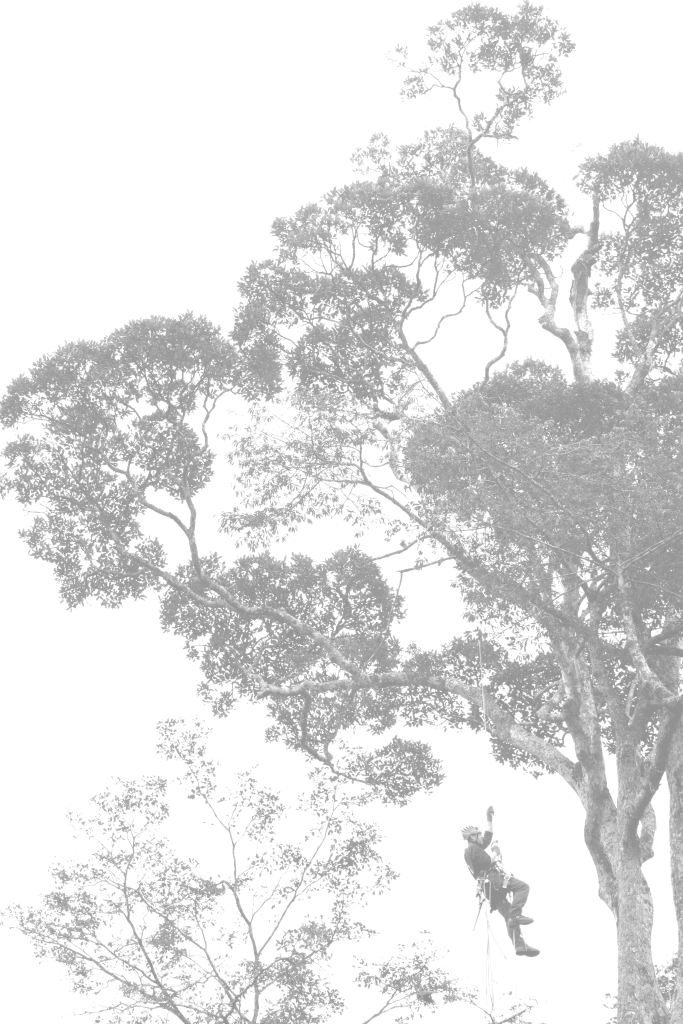
\includegraphics[width=10cm]{Filigrane}
	 \end{textblock}
	\begin{textblock}{140}[0, 1](50, 262)
		\normalfont	Version: \thedate
	\end{textblock}
	\newpage
	~\\ % Print a character or the page will not exist
	\begin{textblock}{140}(40, 40)
		#1
	\end{textblock}
	\begin{textblock}{140}[0,1](40, 270)
		\centering
    
\includegraphics[width=5cm]{Logo-Lab}\\ \bigskip
		UMR \'Ecologie des forêts de Guyane\\
		\url{http://www.ecofog.gf}\\[3\baselineskip]
		Les opinions émises par les auteurs sont personnelles et n’engagent ni l’UMR EcoFoG ni ses tutelles.

    \tiny{Photographie en couverture: Hadrien Lalagüe}
	\end{textblock}
	\newpage
}

% PhD / HDR Thesis
%%%%%%%%%%%%%%%%%%%%%%%%%%%%%%%%%%%%%%%%%%%%%%%%%%%%%%%%%%



% End of preamble
%%%%%%%%%%%%%%%%%%%%%%%%%%%%%%%%%%%%%%%%%%%%%%%%%%%%%%%%%%


\begin{document}
\frontmatter

% Title page
%%%%%%%%%%%%%%%%%%%%%%%%%%%%%%%%%%%%%%%%%%%%%%%%%%%%%%%%%%

\MainTitlePage[Ce document est réalisé de façon dynamique et reproductible grâce à:

\begin{itemize}
  \item \LaTeX, dans sa distribution Miktex (\url{http://miktex.org/}) et la classe memoir (\url{http://www.ctan.org/pkg/memoir}).
  \item R (\url{http://www.r-project.org/}) et RStudio (\url{http://www.rstudio.com/})
  \item bookdown (\url{http://bookdown.org/})
\end{itemize}

Son code source est sur GitHub: \url{https://github.com/EricMarcon/MesuresBioDiv2/}.

Le texte mis à jour en continu peut être lu sur \url{https://ericmarcon.github.io/MesuresBioDiv2/}.

Les versions d'étape sont déposées sur HAL: \url{https://hal-agroparistech.archives-ouvertes.fr/cel-01205813/}.]





% Before Body
%%%%%%%%%%%%%%%%%%%%%%%%%%%%%%%%%%%%%%%%%%%%%%%%%%%%%%%%%%




% Contents
%%%%%%%%%%%%%%%%%%%%%%%%%%%%%%%%%%%%%%%%%%%%%%%%%%%%%%%%%%

\LargeMargins
{
\hypersetup{linkcolor=}
\setcounter{tocdepth}{3}
\tableofcontents
}


% Body
%%%%%%%%%%%%%%%%%%%%%%%%%%%%%%%%%%%%%%%%%%%%%%%%%%%%%%%%%%

\LargeMargins
\hypertarget{motivation}{%
\chapter*{Motivation}\label{motivation}}
\addcontentsline{toc}{chapter}{Motivation}

Le terme \emph{biodiversity} est attribué \autocite{Meine2006} à Walter Rosen, un membre du \emph{National Research Council} américain, qui a commencé à contracter les termes \emph{biological diversity} pendant la préparation d'un colloque dont les actes seront publiés sous le titre ``Biodiversity'' \autocite{Wilson1988}.
La question de la diversité biologique intéressait les écologues bien avant l'invention de la biodiversité, mais le néologisme a connu un succès fulgurant \autocite{Blandin2014} en même temps qu'il devenait une notion floue, dans lequel chacun peut placer ce qu'il souhaite y trouver, au point de lui retirer son caractère scientifique \autocite{Delord2014}.
Une cause de ce glissement est que la biodiversité a été nommée pour attirer l'attention sur son érosion, en lien avec la biologie de la conservation.
Cette érosion concernant potentiellement de nombreux aspects du monde vivant, la définition de la biodiversité fluctue selon les besoins: \textcite{DeLong1996} en recense 85 dans les dix premières années de littérature.
Les indicateurs de la biodiversité peuvent englober bien d'autres choses que la diversité du vivant: le nombre d'espèces menacées (par exemple la liste rouge de l'IUCN), la taille des populations ou la surface des écosystèmes préservés, la dégradation des habitats, la menace pesant sur des espèces emblématiques\ldots{}
Une mesure rigoureuse et cohérente de la diversité peut pourtant être construite pour clarifier beaucoup (mais pas tous) des concepts qui constituent la biodiversité.

Dans l'introduction du premier chapitre des actes de ce qui était devenu le ``Forum sur la Biodiversité'', Wilson utilise le mot dans le sens étroit de nombres d'espèces.
L'élargissement de la notion aux ``systèmes naturels'' et à l'opposé à la diversité génétique intraspécifique est venu du monde de la conservation \autocite{Speth1992}.
La déclaration de Michel Loreau, président du du comité scientifique de la conférence de Paris en 2005 \autocite{Loreau2005} en donne une définition aboutie:

\begin{quote}
La Terre abrite une extraordinaire diversité biologique, qui inclut non seulement les espèces qui habitent notre planète, mais aussi la diversité de leurs gènes, la multitude des interactions écologiques entre elles et avec leur environnement physique, et la variété des écosystèmes complexes qu'elles constituent. Cette biodiversité, qui est le produit de plus de 3 milliards d'années d'évolution, constitue un patrimoine naturel et une ressource vitale dont l'humanité dépend de multiples façons.
\end{quote}

Aujourd'hui encore, le terme \emph{biodiversité} concerne le plus souvent la richesse en espèces d'un écosystème.
Pour simplifier la présentation, le niveau d'étude dans ce document sera en général celui des espèces \autocite[autre concept flou,][]{Hey2001}.
La prise en compte de la totalité des êtres vivants est généralement hors de portée.
La mesure de diversité est alors limitée à un taxocène, c'est-à-dire un sous-ensemble des espèces d'une communauté reliées taxonomiquement: les papillons, les mammifères, les arbres (la délimitation du sous-ensemble n'est pas forcément strictement taxonomique)\ldots{}

Un objet privilégié des études sur la biodiversité est, depuis le Forum, la forêt tropicale parce qu'elle est très diverse et un enjeu pour la conservation.
La plupart des exemples concerneront ici les arbres de la forêt tropicale, qui ont l'avantage d'être clairement définis en tant qu'individus (donc simples à compter) et posent des problèmes méthodologiques considérables pour l'estimation de leur diversité à partir de données réelles.

On peut bien évidemment s'intéresser à d'autres niveaux et d'autres objets, par exemple la diversité génétique (en termes d'allèles différents pour certains gènes ou marqueurs) à l'intérieur d'une population, ou même la diversité des interactions entre espèces d'une communauté \autocite{Jizhong1991}.
On gardera toujours à l'esprit que la prise en compte de la diversité spécifique n'est pas la seule approche, les méthodes présentées ici s'appliquent à la mesure de la diversité en général, pas même nécessairement biologique.

L'objectif de ce document est de traiter la mesure de la biodiversité, pas son importance en tant que telle.
On se référera par exemple à \textcite{Chapin2000} pour une revue sur cette question, \textcite{Cardinale2012} pour les conséquences de l'érosion de la biodiversité sur les services écosystémiques ou \textcite{Ceballos2017} pour les propriétés autocatalytiques de la biodiversité.

La mesure de la diversité est un sujet important en tant que tel \autocite{Purvis2000}, pour permettre de formaliser les concepts et de les appliquer à la réalité.
La question est loin d'être épuisée, et fait toujours l'objet d'une recherche active et de controverses \autocite{Ricotta2005b}.

\hypertarget{notations}{%
\chapter*{Notations}\label{notations}}
\addcontentsline{toc}{chapter}{Notations}

Les notations mathématiques peuvent différer de celles de la littérature citée pour l'homogénéité de ce document.

Les matrices sont notées en caractères gras et majuscules: \(\mathbf{X}\).
Les éléments de la matrice \(\mathbf{X}\) sont notés \(x_{i,j}\).

Les vecteurs sont notés en gras minuscule: \(\mathbf{p}\).
Les nombres sont notés en minuscules, \(n\), et les variables aléatoires en majuscules: \(N\).
Les valeurs maximales des énumérations font exception: elles sont notées en majuscules pour les distinguer des indices: \(\sum_{s=1}^{S}{p_s}=1\).

Le produit matriciel de \(\mathbf{X}\) et \(\mathbf{Y}\) est noté \(\mathbf{X}\mathbf{Y}\). Dans les scripts R, l'opérateur est \texttt{\%*\%}.
Le produit de Hadamard (terme à terme) est noté \(\mathbf{X}\circ\mathbf{Y}\) (opérateur \texttt{*} dans R).
De même \(\mathbf{X}^n\) indique la puissance \(n\) au sens du produit matriciel d'une matrice carrée (opérateur \texttt{\%\^{}\%} du package \emph{expm}), alors que \(\mathbf{X}^{\circ n}\) est la matrice dont chaque terme est celui de \(\mathbf{X}\) à la puissance \(n\) (opérateur \texttt{\^{}} de R).
La matrice transposée de \(\mathbf{X}\) est notée \(\mathbf{X'}\).

Les notations sont les suivantes:

\noindent \({\mathbf 1}(\cdot)\): la fonction indicatrice, qui vaut 1 si la condition dans la parenthèse est vraie, 0 sinon.

\noindent \(\mathbf{1}_s\): le vecteur de longueur \(s\) composé uniquement de 1. \(\mathbf{1}_s\mathbf{1}_s'=\mathbf{J}_s\) où \(\mathbf{J}_s\) est la matrice carré de taille \(s\) ne contenant que des 1.

\noindent \(A\): l'aire d'étude, et, selon le contexte, sa surface.

\noindent \(\alpha_\nu\): la probabilité moyenne des espèces représentées par \(\nu\) individus.

\noindent \(C\): le taux de couverture de l'échantillon, c'est-à-dire la probabilité qu'un individu de la communauté appartienne à une des espèces échantillonnées.
\(C^{n}\) est le taux de couverture correspondant à un échantillon de taille \(n\).

\noindent \(^{q}\!D\): la diversité vraie (nombre de Hill pour les diversités \(\alpha\) et \(\gamma\)), nombre équivalent de communautés pour la diversité \(\beta\).
\(^{q}_{i}\!D_{\alpha}\) est la diversité \(\alpha\) mesurée dans la communauté \(i\).
\(^{q}\!\bar{D}\left(T\right)\) est la diversité phylogénétique.

\noindent \(\boldsymbol{\Delta}\): la matrice de dissimilarité dont les éléments sont \(\delta_{s,t}\), la dissimilarité entre l'espèce \(s\) et l'espèce \(t\).

\noindent \({\mathbb E}\left(X\right)\): l'espérance de la variable aléatoire \(X\).

\noindent \(^{q}\!H\): l'entropie de Tsallis (ou HCDT).
\(^{q}_{i}\!H_{\alpha}\) est l'entropie \(\alpha\) mesurée dans la communauté \(i\).
Si nécessaire, le vecteur des probabilités servant au calcul est précisé sous la forme \(^{q}\!H(\mathbf{p})\).
\(^{q}\!\bar{H}(T)\) est l'entropie phylogénétique.

\noindent \(I\): le nombre de communautés qui constituent une partition de la méta-communauté dans le cadre de la décomposition de la diversité.
Les communautés sont indexées par \(i\).

\noindent \(I(p_s)\): l'information apportée par l'observation d'un évènement de probabilité \(p_s\).
\(I(q_s,p_s)\) est le gain d'information apporté par l'expérience (\(q_s\) est observé) par rapport aux probabilités \(p_s\) attendues.

\noindent \(\mathbf{I}_s\): la matrice identité de rang \(s\): matrice carrée de taille \(s\times s\) dont la diagonale ne comporte que des 1 et les autres élements sont nuls.

\noindent \(N\): le nombre (aléatoire) d'individus se trouvant dans l'aire d'étude.
\(N_s\) est la même variable aléatoire, mais restreinte aux individus de l'espèce \(s\).

\noindent \(n\): le nombre d'individus échantillonnés.
\(n_{s,i}\) est le nombre d'individus de l'espèce \(s\) dans la communauté \(i\).
Les effectifs totaux sont \(n_{s+}\) (pour l'espèce \(s\)), \(n_{+i}\) pour la communauté \(i\) et \(n\) le total général.
S'il n'y a qu'une communauté, le nombre d'individus par espèce est \(n_s\).

\noindent \(p_s\): la probabilité qu'un individu tiré au hasard appartienne à l'espèce \(s\).
Son estimateur, \({\hat{p}}_s\) est la fréquence observée.
\(p_{s|i}\) est la même probabilité dans la communauté \(i\).

\noindent \(\mathbf{p}=\left( p_1, p_2, \dots, p_s, \dots, p_S \right)\): le vecteur décrivant la distribution des probabilités \(p_s\), appelé simplexe en référence à sa représentation dans l'espace à \(S\) dimensions.

\noindent \({\pi}_{\nu}\): la probabilité qu'une espèce choisie au hasard soit représentée par \(\nu\) individus, \(\sum^n_{\nu=1}{{\pi}_{\nu}}\)=1.
Si l'espèce est choisie explicitement, la probabilité est notée \({\pi}_{n_s}\).

\noindent \(^{q}\!R\): l'entropie de Rényi d'ordre \(q\).

\noindent \(S\): le nombre d'espèces, considéré comme une variable aléatoire, estimé par \(\hat{S}\).

\noindent \(S^{n}_{\nu}\): le nombre d'espèces, considéré comme une variable aléatoire, observées \(\nu\) fois dans l'échantillonnage.
L'indice est le nombre de fois où l'espèce est détectée: par exemple \(S_{1}\) ou \(S_{\ne 0}\).
L'exposant est la taille de l'échantillon: \(S^{A}\) pour la surface \(A\) ou \(\hat{S}^{n}\) pour un échantillon de \(n\) individus.
\(S^{A}_{0}\) est le nombre d'espèces non rencontrées dans la surface \(A\).
Pour alléger les notations, s'il n'y a pas d'ambiguïté, l'indice est omis pour les espèces présentes: \(S^{A}_{\ne 0}\) est noté \(S^{A}\).
Si l'exposant n'est pas noté, l'échantillon n'est pas précisé et peut être aussi bien un nombre d'individus qu'une surface.

\noindent \(s^{n}_{\nu}\): le nombre d'espèces observées, avec les mêmes notations que ci-dessus.
\(s^{n}_{\nu}\) peut être considéré comme une réalisation de \(S^{n}_{\nu}\).

\noindent \(t^{n}_{1-\alpha/2}\): le quantile d'une loi de Student à \(n\) degrés de liberté au seuil de risque \(\alpha\), classiquement 1,96 pour \(n\) grand et \(\alpha=5\%\).

\noindent \(\mathbf{Z}\): la matrice de similarité entre espèces dont les éléments sont \(z_{s,t}\), la similarité entre l'espèce \(s\) et l'espèce \(t\).

\noindent \(\mathrm{\Gamma}(\cdot)\): la fonction gamma.

\noindent \(\mathrm{\Psi}(\cdot)\): la fonction digamma.

\noindent \(\binom{n}{k}\): le nombre de combinaisons de \(k\) éléments parmi \(n\): \[\binom{n}{k}=\frac{n!}{k!\,(n-k)!}\].

\mainmatter

\hypertarget{part-notions}{%
\part{Notions}\label{part-notions}}

\hypertarget{notions-de-diversituxe9}{%
\chapter{Notions de Diversité}\label{notions-de-diversituxe9}}

\scriptsize

\normalsize

\hypertarget{composantes}{%
\section{Composantes}\label{composantes}}



\scriptsize

\begin{SCfigure}

{\centering 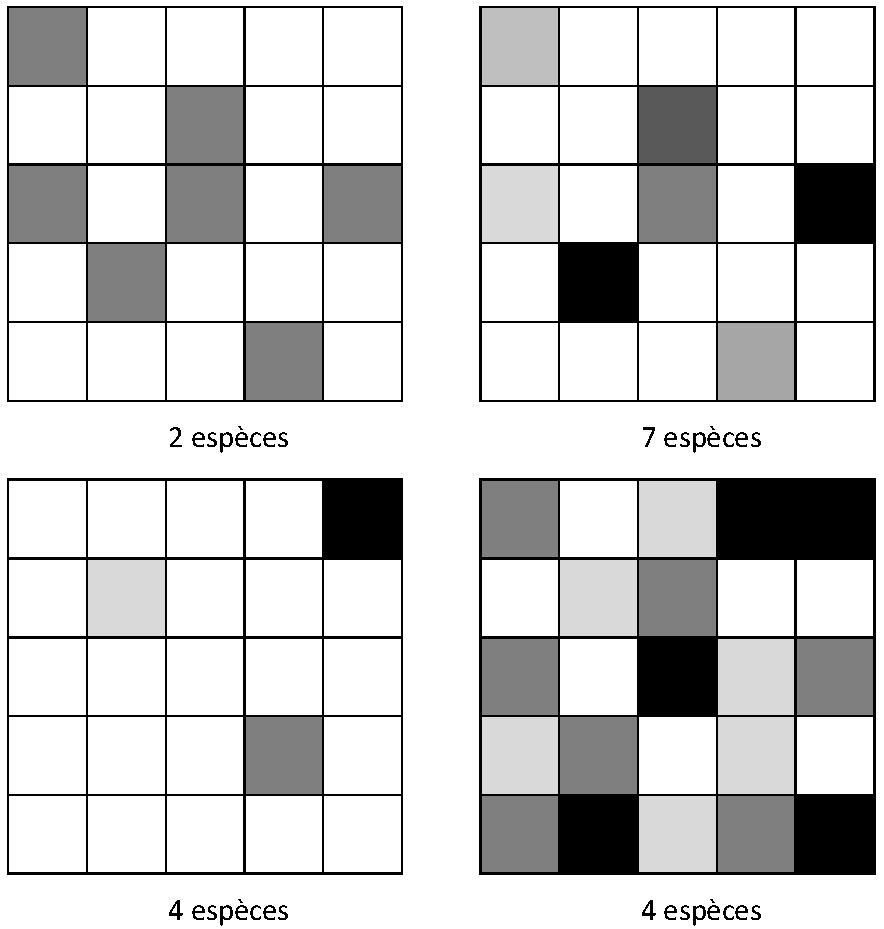
\includegraphics[width=0.6\linewidth]{images/Composantes} 

}

\caption{Importance de la richesse (en haut) et de l'équitabilité (en bas) pour la définition de la diversité. Ligne du haut: toutes choses égales par ailleurs, une communauté de 7 espèces semble plus diverse qu'une communauté de 2 espèces. Ligne du bas: à richesse égale, une communauté moins équitable (à gauche) semble moins diverse. Colonne de gauche: une communauté moins riche (en haut) peut sembler plus diverse si elle est plus équitable. Colonne de droite: idem pour la communauté du bas.}\label{fig:Composantes}
\end{SCfigure}

\normalsize

Une communauté comprenant beaucoup d'espèces mais avec une espèce dominante n'est pas perçue intuitivement comme plus diverse qu'une communauté avec moins d'espèces, mais dont les effectifs sont proches (figure \ref{fig:Composantes}, colonne de gauche).
La prise en compte de deux composantes de la diversité, appelées richesse et équitabilité, est nécessaire \autocite{Whittaker1965}.

\hypertarget{richesse}{%
\subsection{Richesse}\label{richesse}}

La richesse \autocite[terme introduit par][]{Mcintosh1967} est le nombre (ou une fonction croissante du nombre) de classes différentes présentes dans le système étudié, par exemple le nombre d'espèces d'arbres dans une forêt.

Un certain nombre d'hypothèses sont assumées plus ou moins explicitement:

\begin{itemize}
\tightlist
\item
  Les classes sont bien connues: compter le nombre d'espèces a peu de sens si la taxonomie n'est pas bien établie.
  C'est parfois une difficulté majeure quand on travaille sur les microorganismes;
\item
  Les classes sont équidistantes: la richesse augmente d'une unité quand on rajoute une espèce, que cette espèce soit proche des précédentes ou extrêmement originale.
\end{itemize}

L'indice de richesse le plus simple et le plus utilisé est tout simplement le nombre d'espèces \(S\).

\hypertarget{uxe9quitabilituxe9}{%
\subsection{Équitabilité}\label{uxe9quitabilituxe9}}

La régularité de la distribution des espèces (équitabilité en Français, \emph{evenness} ou \emph{equitability} en anglais) est un élément important de la diversité.
Une espèce représentée abondamment ou par un seul individu n'apporte pas la même contribution à l'écosystème.
Sur la figure \ref{fig:Composantes}, la ligne du bas présente deux communautés de 4 espèces, mais celle de droite est beaucoup plus équitable de celle de gauche et semble intuitivement plus diverse.
À nombre d'espèces égal, la présence d'espèces très dominantes entraîne mathématiquement la rareté de certaines autres: on comprend donc assez intuitivement que le maximum de diversité sera atteint quand les espèces auront une répartition très régulière.

Un indice d'équitabilité est indépendant du nombre d'espèces (donc de la richesse).

La plupart des indices courants, comme ceux de Simpson ou de Shannon, évaluent à la fois la richesse et l'équitabilité.

\hypertarget{disparituxe9}{%
\subsection{Disparité}\label{disparituxe9}}

Les mesures classiques de la diversité, dites mesures de diversité neutre (\emph{species-neutral diversity}) ou taxonomique ne prennent pas en compte une quelconque distance entre classes.
Pourtant, deux espèces du même genre sont de toute évidence plus proches que deux espèces de familles différentes.
Les mesures de diversité phylogénétique et de diversité fonctionnelle prennent en compte cette notion, qui nécessite quelques définitions supplémentaires \autocite{Mouillot2005,Ricotta2007}.

La mesure de la différence entre deux classes est souvent une distance, mais parfois une mesure qui n'a pas toutes les propriétés d'une distance: une dissimilarité.
Les mesures de \emph{divergence} \autocite{Pavoine2011} sont construites à partir de la dissimilarité entre les classes, avec ou sans pondération par la fréquence.

La disparité \autocite{Runnegar1987}, divergence moyenne entre deux espèces (indépendamment des fréquences), ou de façon équivalente la longueur totale des branches d'un arbre phylogénétique, est la composante qui décrit à quel point les espèces sont différentes les unes des autres.

Les mesures de \emph{régularité} décrivent la façon dont les espèces occupent l'espace des niches (régularité fonctionnelle) ou la régularité dans le temps et entre les clades des évènements de spéciation représentés par un arbre phylogénétique.
Ce concept complète celui d'équitabilité dans les mesures classiques: la diversité augmente avec la richesse, la divergence entre espèces, et la régularité (qui se réduit à l'équitabilité quand toutes les espèces sont également divergentes entre elles).

\hypertarget{agruxe9gation}{%
\subsection{Agrégation}\label{agruxe9gation}}

À partir d'une large revue de la littérature dans plusieurs disciplines scientifiques s'intéressant à la diversité (au-delà de la biodiversité), \textcite{Stirling2007} estime que les trois composantes, qu'il nomme \emph{variété} (richesse), \emph{équilibre} (équitabilité) et \emph{disparité}, recouvrent tous les aspects de la diversité.

Stirling définit la propriété d'\emph{agrégation} comme la capacité d'une mesure de diversité à combiner explicitement les trois composantes précédentes.
Cela ne signifie pas que les composantes contribuent indépendamment les unes des autres à la diversité \autocite{Jost2010}.

\hypertarget{niveaux-de-luxe9tude}{%
\section{Niveaux de l'étude}\label{niveaux-de-luxe9tude}}

La diversité est classiquement estimée à plusieurs niveaux emboîtés, nommés \(\alpha\), \(\beta\) et \(\gamma\) par \textcite[page 320]{Whittaker1960} qui a nommé \(\alpha\) la diversité locale qu'il mesurait avec l'indice \(\alpha\) de Fisher (voir le chapitre \ref{chap:Fisher}) et a utilisé les lettres suivantes selon ses besoins.

\hypertarget{diversituxe9-alpha-beta-et-gamma}{%
\subsection{\texorpdfstring{Diversité \(\alpha\), \(\beta\) et \(\gamma\)}{Diversité \textbackslash alpha, \textbackslash beta et \textbackslash gamma}}\label{diversituxe9-alpha-beta-et-gamma}}

La diversité \(\alpha\) est la diversité locale, mesurée à l'intérieur d'un système délimité.
Plus précisément, il s'agit de la diversité dans un habitat uniforme de taille fixe.



\scriptsize

\begin{SCfigure}

{\centering 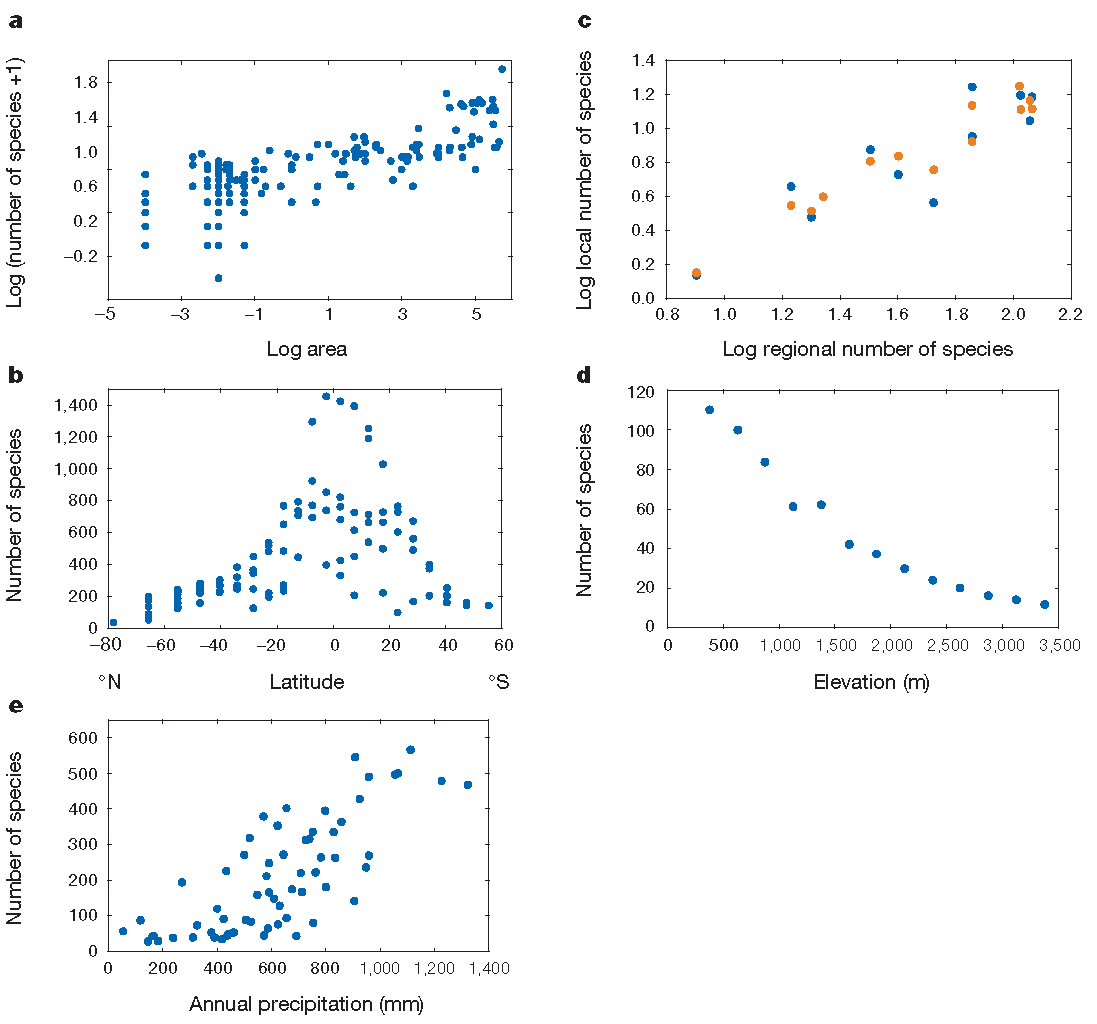
\includegraphics[width=1\linewidth]{images/Gaston2000} 

}

\caption{Patrons de biodiversité. (a) Le nombre d'espèces de vers de terre augmente en fonction de la surface échantillonnée, de 100 m² à plus de 500000 km² selon la relation d'Arrhenius). (b) Nombre d'espèces d'oiseaux en fonction de la latitude. (c) Relation entre la richesse régionale et la richesse locale. (d) Nombre d'espèces de chauves-souris en fonction de l'altitude dans une réserve au Pérou. (e) Nombre d'espèces de végétaux ligneux en fonction des précipitations en Afrique du Sud.}\label{fig:Gaston2000}
\end{SCfigure}

\normalsize

De façon générale \autocite{Gaston2000}, la richesse spécifique diminue avec la latitude (la diversité est plus grande dans les zones tropicales, et au sein de celles-ci, quand on se rapproche de l'équateur), voir figure \ref{fig:Gaston2000} \autocite[figure 1]{Gaston2000}.
La tendance est la même pour la diversité génétique intraspécifique \autocite{Miraldo2016}.
La richesse diminue avec l'altitude.
Elle est généralement plus faible sur les îles, où elle décroît avec la distance au continent, source de migrations.

La diversité \(\beta\) mesure à quel point les systèmes locaux sont différents. Cette définition assez vague fait toujours l'objet de débats \autocite{Moreno2010}.

Enfin, la diversité \(\gamma\) est similaire à la diversité \(\alpha\), prise en compte sur l'ensemble du système étudié.
Les diversités \(\alpha\) et \(\gamma\) se mesurent donc de la même façon.

\hypertarget{duxe9composition}{%
\subsection{Décomposition}\label{duxe9composition}}

\textcite{Whittaker1977} a proposé sans succès une normalisation des échelles d'évaluation de la biodiversité, en introduisant la diversité régionale \(\varepsilon\) (\(\gamma\) étant réservé au paysage et \(\alpha\) à l'habitat) et la diversité \(\delta\) entre les paysages.
Seuls les trois niveaux originaux ont été conservés par la littérature, sans définition stricte des échelles d'observation.

La distinction entre les diversités \(\alpha\) et \(\beta\) dépend de la finesse de la définition de l'habitat.
La distinction de nombreux habitats diminue la diversité \(\alpha\) au profit de la \(\beta\).
Il est donc important de définir une mesure qui ne dépende pas de ce découpage, donc une mesure cumulative (additive ou multiplicative) décrivant la diversité totale, décomposable en la somme ou le produit convenablement pondérés de toutes les diversités \(\alpha\) des habitats (diversité intra) et de la diversité \(\beta\) inter-habitat.

Nous appellerons \emph{communauté} le niveau de découpage concernant la diversité \(\alpha\) et \emph{méta-communauté} le niveau de regroupement pour l'estimation de la diversité \(\gamma\).

\hypertarget{le-probluxe8me-de-lespuxe8ce}{%
\section{Le problème de l'espèce}\label{le-probluxe8me-de-lespuxe8ce}}

Évaluer la richesse spécifique suppose que les espèces soient définies clairement, ce qui n'est de toute évidence pas le cas \autocite{Casetta2014a}.
Le premier aspect du problème concerne la nature des espèces: réalité naturelle ou seulement représentation simplificatrice.
Une analyse historique et philosophique en est faite par \textcite{Richards2010}.
L'autre aspect, avec des conséquences pratiques plus immédiates, concerne leur délimitation.
\textcite{Mayden1997} recense 22 définitions différentes du concept d'espèce.

Le concept le plus répandu est celui d'espèce \emph{biologique} \autocite{Dobzhansky1937}: un ``groupe de populations naturelles isolées reproductivement les unes des autres'' \autocite{Mayr1942}.
Lorsque les populations d'une espèce sont isolées géographiquement, leur capacité à se reproduire ensemble est toute théorique (et d'ailleurs rarement vérifiée expérimentalement).
Des populations allopatriques n'ont pas de flux de gènes réels entre elles et peuvent être considérées comme des espèces distinctes selon le concept d'espèce \emph{phylogénétique}: ``le plus petit groupe identifiable d'individus avec un pattern commun d'ancêtres et de descendants'' \autocite{Cracraft1983}.
C'est l'unité génétique détectée par la méthode du coalescent pour la délimitation des espèces \autocite{Sukumaran2017}.
Le nombre d'espèces phylogénétiques est bien supérieur au nombre d'espèces biologiques.
Enfin, \textcite{VanValen1976} définit les espèces par la niche écologique qu'elles occupent (à partir de l'exemple des chênes blancs européens) plutôt que par les flux de gènes (permanents entre les espèces distinctes): le concept \emph{écologique} d'espèce est proche de celui de complexe d'espèces \autocite[ensemble d'espèces voisines échangeant des gènes,][]{Pernes1984}.

Le choix de la définition modifie considérablement sur la quantification de la richesse \autocite{Agapow2004}.
Des problèmes méthodologiques s'ajoutent aux problèmes conceptuels \autocite{Hey2001}: la séparation ou le regroupement de plusieurs populations ou morphotypes en un nombre plus ou moins grand d'espèces est un choix qui reflète les connaissances du moment et peut évoluer \autocite{Barberousse2014}.

L'impact du problème de l'espèce sur la mesure de la diversité reste sans solution à ce stade, si ce n'est d'utiliser les mêmes définitions si des communautés différentes doivent être comparées.
L'approche phylogénétique (Chapitre \ref{chap:Phyloentropie}) permet de contourner le problème: si deux taxons très semblables apportent à peine plus de diversité qu'un seul taxon, le choix de les distinguer ou non n'est pas critique.

\hypertarget{outils}{%
\chapter{Outils}\label{outils}}

\scriptsize

\begin{Essentiel}
La diversité peut être décrite localement par une courbe d'accumulation
(SAC) qui représente le nombre d'espèces échantillonnées en fonction de
l'effort. À une échelle plus large, cette courbe s'appelle relation
aire-espèces (SAR).

La distribution des abondances des espèces (SAD) est représentée par une
histogramme des fréquences ou un diagramme rang-abondance.

Le taux de couverture est la somme des probabilités des espèces
observées étant donné l'effort d'échantillonnage. Il peut être estimé
précisément à partir des données d'inventaire. Le taux de complétude est
la proportion (en nombre) des espèces observées.
\end{Essentiel}

\normalsize

Quelques outils sont nécessaires avant d'entrer dans le coeur du sujet.
Les relations décrivant le nombre d'espèces en fonction de la taille de l'échantillon (relations aire-espèces) et la distribution de l'abondance des espèces sont importants pour les écologues.
La mesure de l'exhaustivité de l'échantillonnage par le taux de couverture sera la base de l'estimation de la diversité à partir de données réelles.

\hypertarget{calculs-et-donnuxe9es}{%
\section{Calculs et données}\label{calculs-et-donnuxe9es}}

La présentation des mesures de diversité est donnée avec un usage intensif du formalisme mathématique.
La liste des notations est fournie en préambule du document, on s'y référera autant que nécessaire.

Les calculs sont réalisés dans R \autocite{R}, essentiellement avec le package \emph{entropart} \autocite{Marcon2014c}.
L'ensemble du code est disponible sur GitHub\footnote{\url{https://github.com/EricMarcon/MesuresBioDiv2/}} où se trouvent les mises à jour de ce document \footnote{\url{https://ericmarcon.github.io/MesuresBioDiv2/}}.

Les données sont souvent celles de la parcelle 6 de Paracou en Guyane française \autocite{Gourlet-Fleury2004}, d'une surface de 6.25~ha.
Tous les arbres de plus de 10~cm de diamètre à hauteur de poitrine (DBH: \emph{Diameter at Breast Height}) y ont été inventoriés en 2016.
La postition de chaque arbre, son espèce et sa surface terrière sont fournis dans le package \emph{SpatDiv}.

D'autres exemples utilisent la parcelle forestière permanente de Barro Colorado Island, souvent abrégée BCI \autocite{Condit2012}: 50~ha de forêt tropicale dont les arbres de plus de 1~cm de diamètre à hauteur de poitrine (DBH: \emph{Diameter at Breast Height}) ont été inventoriés.
Le jeu de données utilisé pour les exemples est une version réduite aux arbres de plus de 10~cm disponible dans le package \emph{vegan} \autocite{Oksanen2012}.

\hypertarget{sad-et-sar}{%
\section{SAD et SAR}\label{sad-et-sar}}



\scriptsize

\begin{SCfigure}

{\centering 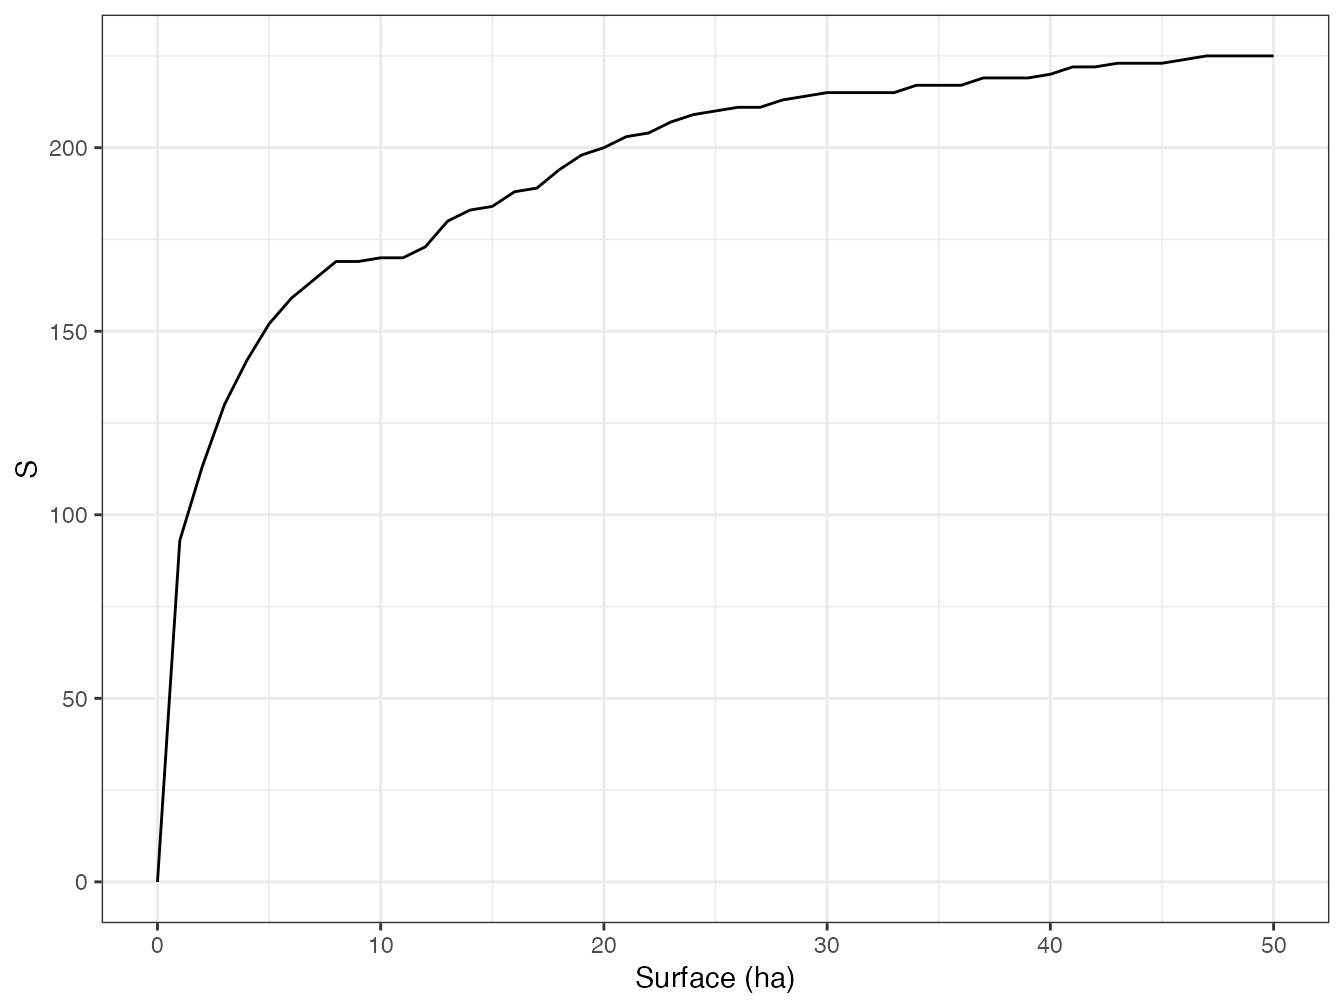
\includegraphics[width=0.8\linewidth]{MesuresBD_files/figure-latex/SARFig-1} 

}

\caption{Courbe d'accumulation des espèces d'arbres du dispositif de Barro Colorado Island. Le nombre d'espèces est cumulé dans l'ordre des carrés d'un hectare du dispositif.}\label{fig:SARFig}
\end{SCfigure}

\normalsize

La courbe aire-espèces (SAR: \emph{Species Area Relationship}) représente le nombre d'espèces observées en fonction de la surface échantillonnée (figure \ref{fig:Williamson2001}).
Il existe plusieurs façons de prendre en compte cette relation \autocite{Scheiner2003}, classables en deux grandes familles \autocite{Dengler2009}:

\begin{itemize}
\tightlist
\item
  Dans une SAR au sens strict, chaque point représente une communauté.
  La question traitée est la relation entre le nombre d'espèces et la taille de chaque communauté;
\item
  Si les points représentent un effort d'échantillonnage différent dans même communauté, on parle de courbe d'accumulation (SAC: \emph{Species Acumulation Curve}). Une courbe de raréfaction (\emph{Rarefaction Curve}) peut être calculée en réduisant par des outils statistiques l'effort d'échantillonnage réel pour obtenir une SAC théorique, libérée des aléas de l'ordre de prise en compte des données.
\end{itemize}

La figure \ref{fig:SARFig} montre l'accumulation des espèces pour les données de BCI.
Une SAC peut être tracée en fonction de la surface, du nombre d'individus ou du nombres de placettes d'échantillonnage, selon les besoins.

Code R pour réaliser la figure \ref{fig:SARFig}:

\scriptsize

\begin{Shaded}
\begin{Highlighting}[]
\KeywordTok{library}\NormalTok{(}\StringTok{"vegan"}\NormalTok{)}
\KeywordTok{data}\NormalTok{(BCI)}
\NormalTok{Cumul <-}\StringTok{ }\KeywordTok{apply}\NormalTok{(BCI, }\DecValTok{2}\NormalTok{, cumsum)}
\NormalTok{Richesse <-}\StringTok{ }\KeywordTok{apply}\NormalTok{(Cumul, }\DecValTok{1}\NormalTok{, }\ControlFlowTok{function}\NormalTok{(x) }\KeywordTok{sum}\NormalTok{(x }\OperatorTok{>}\StringTok{ }\DecValTok{0}\NormalTok{))}
\NormalTok{SARplot <-}\StringTok{ }\KeywordTok{ggplot}\NormalTok{(}\KeywordTok{data.frame}\NormalTok{(}\DataTypeTok{A =} \DecValTok{0}\OperatorTok{:}\DecValTok{50}\NormalTok{, }
                             \DataTypeTok{S =} \KeywordTok{c}\NormalTok{(}\DecValTok{0}\NormalTok{, Richesse))) }\OperatorTok{+}
\StringTok{  }\KeywordTok{aes}\NormalTok{(A, S) }\OperatorTok{+}
\StringTok{  }\KeywordTok{geom_line}\NormalTok{() }\OperatorTok{+}
\StringTok{  }\KeywordTok{labs}\NormalTok{(}\DataTypeTok{x =} \StringTok{"Surface (ha)"}\NormalTok{)}
\NormalTok{SARplot}
\end{Highlighting}
\end{Shaded}

\normalsize

La distribution de l'abondance des espèces (SAD: \emph{Species Abundance Distribution}) est la loi qui donne l'abondance attendue de chaque espèce d'une communauté.
Les espèces ne sont pas identifiées individuellement, mais par le nombre d'individus leur appartenant.



\scriptsize

\begin{SCfigure}

{\centering 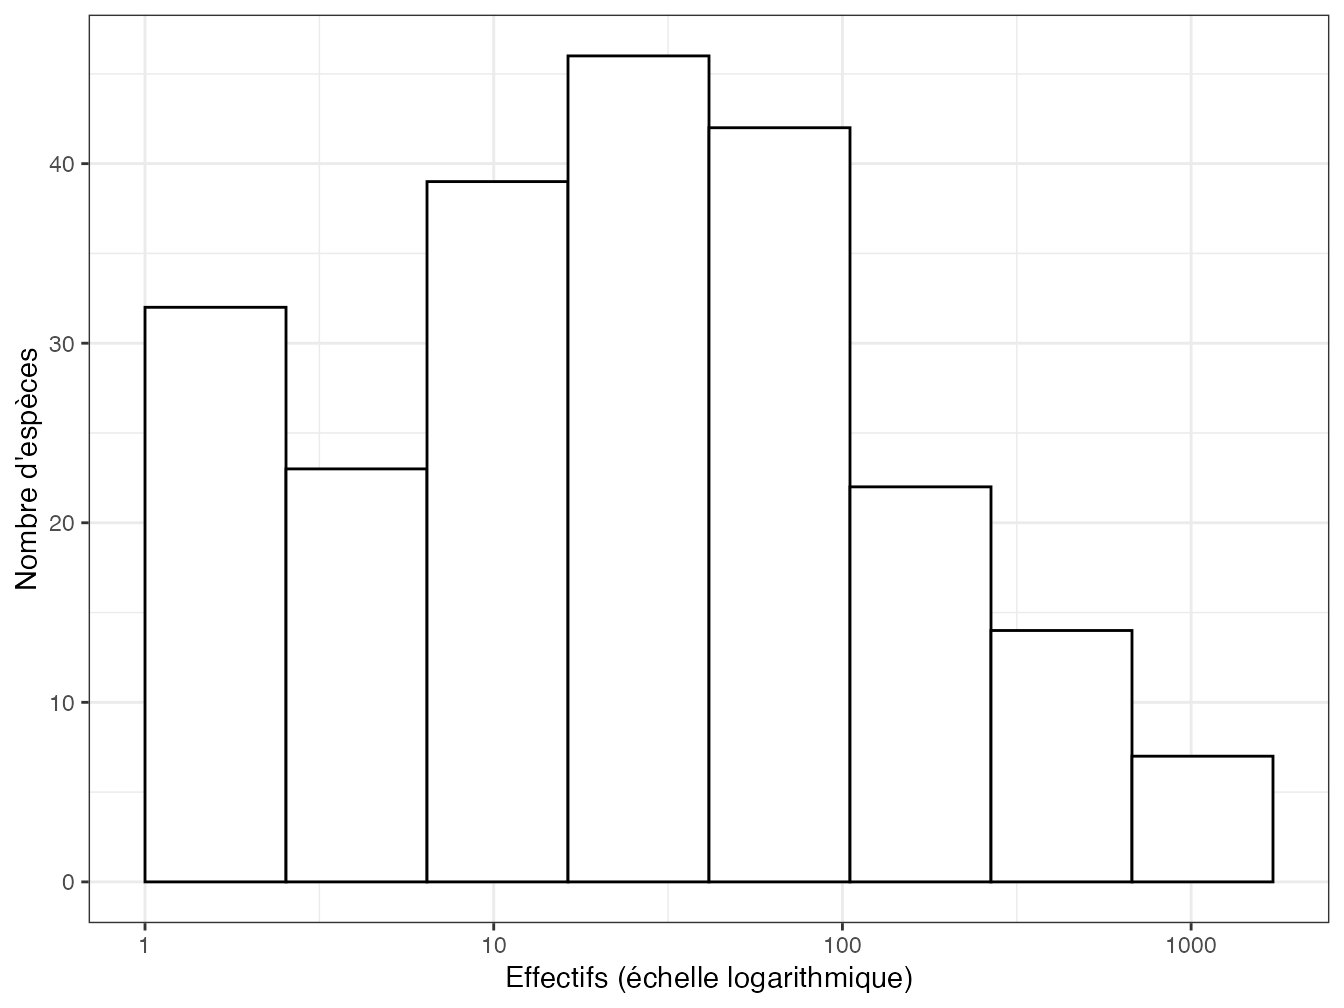
\includegraphics[width=0.8\linewidth]{MesuresBD_files/figure-latex/SADFig-1} 

}

\caption{Histogramme des fréquences (diagramme de Preston) des arbres du dispositif de Barro Colorado Island. En abscisse: le nombre d'arbres de chaque espèce (en logarithme); en ordonnée: le nombre d'espèces.}\label{fig:SADFig}
\end{SCfigure}

\normalsize

Elle peut être représentée sous la forme d'un histogramme des fréquences (diagramme de \textcite{Preston1948}, figure \ref{fig:SADFig}) ou bien d'un diagramme rang-abondance (RAC: \emph{Rank Abundance Curve} ou diagramme de \textcite{Whittaker1965}, figure \ref{fig:RACFig}).
Le RAC est souvent utilisé pour reconnaître des distributions connues.
\textcite{Izsak2012} ont étudié les propriétés des RAC pour les principales SAD.



\scriptsize

\begin{SCfigure}

{\centering 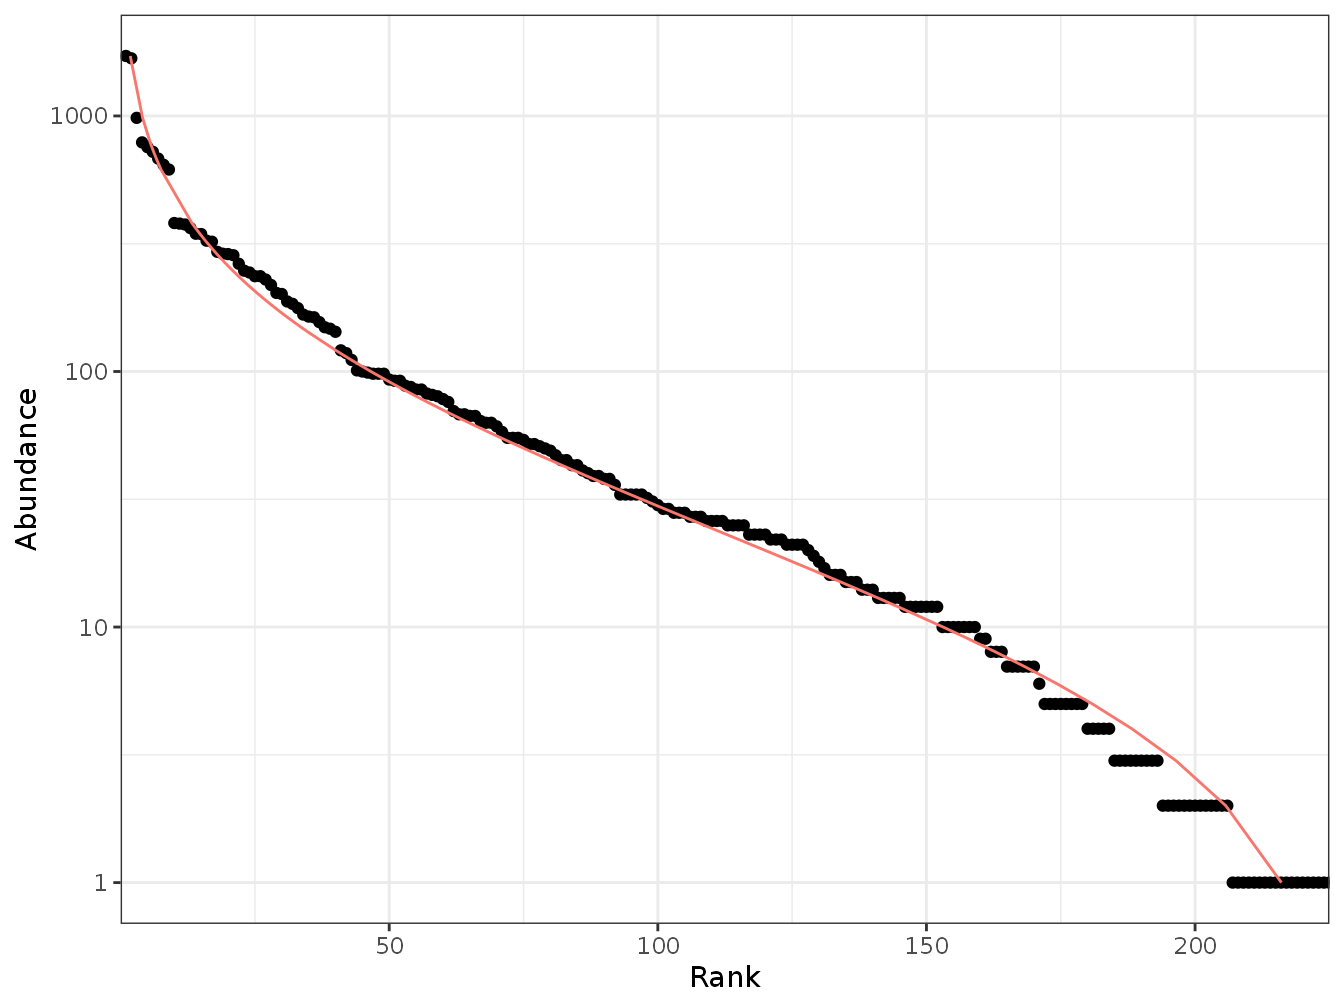
\includegraphics[width=0.8\linewidth]{MesuresBD_files/figure-latex/RACFig-1} 

}

\caption{Diagramme rang-abondance (diagramme de Whittaker) des arbres du dispositif de Barro Colorado Island. Les points sont les données: en abscisse: le rang de l'espèce, à partir de la plus abondante; en ordonnée: l'abondance de l'espèce. La courbe est l'ajustement d'une distribution log-normale.}\label{fig:RACFig}
\end{SCfigure}

\normalsize

Code de la figure \ref{fig:SADFig}:

\scriptsize

\begin{Shaded}
\begin{Highlighting}[]
\NormalTok{Ns <-}\StringTok{ }\KeywordTok{sort}\NormalTok{(}\KeywordTok{colSums}\NormalTok{(BCI), }\DataTypeTok{decr =} \OtherTok{TRUE}\NormalTok{)}
\NormalTok{N <-}\StringTok{ }\KeywordTok{sum}\NormalTok{(Ns)}
\NormalTok{SADhist <-}\StringTok{ }\KeywordTok{ggplot}\NormalTok{(}\KeywordTok{data.frame}\NormalTok{(Ns), }\KeywordTok{aes}\NormalTok{(Ns)) }\OperatorTok{+}\StringTok{ }
\StringTok{  }\KeywordTok{geom_histogram}\NormalTok{(}\DataTypeTok{bins=}\KeywordTok{nclass.Sturges}\NormalTok{(}\KeywordTok{log}\NormalTok{(Ns)), }
       \DataTypeTok{color=}\StringTok{"black"}\NormalTok{, }\DataTypeTok{fill=}\StringTok{"white"}\NormalTok{, }\DataTypeTok{boundary =} \DecValTok{0}\NormalTok{) }\OperatorTok{+}
\StringTok{  }\KeywordTok{scale_x_log10}\NormalTok{() }\OperatorTok{+}
\StringTok{  }\KeywordTok{labs}\NormalTok{(}\DataTypeTok{x=}\StringTok{"Effectifs (échelle logarithmique)"}\NormalTok{, }
       \DataTypeTok{y=}\StringTok{"Nombre d'espèces"}\NormalTok{)}
\NormalTok{SADhist}
\end{Highlighting}
\end{Shaded}

\normalsize

Code de la figure \ref{fig:RACFig}:

\scriptsize

\begin{Shaded}
\begin{Highlighting}[]
\KeywordTok{library}\NormalTok{(}\StringTok{"entropart"}\NormalTok{)}
\KeywordTok{autoplot}\NormalTok{(}\KeywordTok{as.AbdVector}\NormalTok{(Ns), }\DataTypeTok{Distribution =} \StringTok{"lnorm"}\NormalTok{)}
\end{Highlighting}
\end{Shaded}

\normalsize

Les SAD ne sont pas traitées en détail ici: on se reportera à \textcite{Magurran1988}, \textcite{McGill2007} et Izsák et Pavoine.
Les SAD nécessaires à la compréhension de la suite sont:

\begin{itemize}
\tightlist
\item
  La distribution géométrique \autocite{Motomura1932,Whittaker1972};
\item
  La distribution en log-séries de \textcite{Fisher1943};
\item
  La distribution log-normale \autocite{Preston1948};
\item
  Le modèle Broken Stick \autocite{MacArthur1957}.
\end{itemize}

\hypertarget{sec:Couverture}{%
\section{Taux de couverture}\label{sec:Couverture}}

\hypertarget{formule-des-fruxe9quences-de-good-turing}{%
\subsection{Formule des fréquences de Good-Turing}\label{formule-des-fruxe9quences-de-good-turing}}

La relation fondamentale entre les fréquences des espèces est due à Turing et a été publiée par \textcite{Good1953}.
En absence de toute information sur la loi de distribution des espèces, en supposant seulement que les individus sont tirés indépendamment les uns des autres selon une loi multinomiale respectant ces probabilités, la formule de Good-Turing relie la probabilité moyenne \(\alpha_\nu\) d'une espèce représentée \(\nu\) fois (c'est-à-dire par \(\nu\) individus) au rapport entre les nombres d'espèces représentées \(\nu+1\) fois et \(\nu\) fois:

\begin{equation}
  \label{eq:alphanu}
  \alpha_\nu \approx \frac{(\nu+1)}{n} \frac{s^{n}_{\nu+1}}{s^{n}_{\nu}}.
\end{equation}

Les singletons (\(s^{n}_{1}\): le nombre d'espèces observées une seule fois) et les doubletons (\(s^{n}_{2}\): le nombre d'espèces observées deux fois) ont une importance centrale.
Pour \(\nu=1\), on a: \(\alpha_1 = 2 s^{n}_{2}/(ns^{n}_{1})\): la fréquence d'une espèce typiquement représentée par un singleton est proportionnelle au rapport entre le nombre des doubletons et des singletons.
Pour \(\nu=0\), l'ignorance du nombre d'espèces non échantillonnées \(s^{n}_{0}\) pose problème mais le produit \(\alpha_0 \times s^{n}_{0} = \pi_0\), la probabilité totale des espèces non représentées, peut être estimée par \(s^{n}_{1}/n\).
Ces relations sont le fondement des estimateurs de richesse de Chao présentées ci-dessous.

La relation a été précisée \autocite[eq. 6 et 7a]{Chiu2014a} en limitant les approximations dans les calculs.
La seule nécessaire est que les probabilités des espèces représentées le même nombre de fois \(\nu\) varient peu et puissent être considérées toutes égales à \(\alpha_\nu\).
Alors, \(\alpha_\nu\) est estimé par
\begin{equation}
  \label{eq:GoodTuring2014}
  \hat{\alpha}_\nu = \frac{\left(\nu+1 \right) s^{n}_{\nu+1}}{\left(n-\nu \right) s^{n}_{\nu} + \left(\nu+1 \right) s^{n}_{\nu+1}}.
\end{equation}

Ce nouvel estimateur est à la base de l'estimateur de Chao amélioré et des estimateurs d'entropie de Chao et Jost (sections \ref{sec:BiaisShannon} et \ref{sec:BiaisHCDT}).

\hypertarget{taux-de-couverture-et-duxe9ficit-de-couverture}{%
\subsection{Taux de couverture et déficit de couverture}\label{taux-de-couverture-et-duxe9ficit-de-couverture}}

\textcite{Good1953} définit le taux de couverture (\emph{sample coverage}) de l'échantillonnage comme la proportion des espèces découvertes,
\begin{equation}
  \label{eq:C}
  C=\sum^S_{s=1}{{\mathbf 1}\left(n_s>0\right)p_s},
\end{equation}

où \({\mathbf 1}(\cdot)\) est la fonction indicatrice.
Son complément à 1 est appelé déficit de couverture (\emph{coverage deficit}).

Le taux de couverture augmente avec l'effort d'échantillonnage.
Plus il est élevé, meilleures seront les estimations de la diversité.
Pour comparer deux communautés par des courbes de raréfaction, \textcite{Chao2012b} montrent que le taux de couverture plutôt que la taille de l'échantillon doit être identique.
Les estimateurs de la diversité développés plus loin reposent largement sur cette notion pour la correction du biais d'échantillonnage \autocite{Dauby2012} (la sous-estimation systématique de la diversité due aux espèces non observées, un des éléments du biais d'estimation).

L'estimateur du taux de couverture, que Good attribue à Turing, est selon la relation des fréquences vues plus haut:

\begin{equation}
  \label{eq:CGood}
  \hat{C} = 1-\frac{s^{n}_{1}}{n}.
\end{equation}

Cet estimateur est biaisé \autocite{Zhang2007}. En réalité,
\begin{equation}
  \label{eq:CsansBiais}
  C = 1-\frac{{\mathbb E}(S^{n}_{1}) - \pi_1}{n}.
\end{equation}

L'estimateur de Good néglige le terme \(\pi_1\), la somme des probabilités des espèces observées une fois.
Ce terme peut être estimé avec un biais plus petit.
\textcite{Chao1988} puis \textcite{Zhang2007} proposent l'estimateur suivant, qui utilise toute l'information disponible et a le plus petit biais possible:

\begin{equation}
  \label{eq:CZhang}
  \hat{C}=1-\sum^{n}_{\nu=1}{\left(-1\right)}^{\nu+1}{\binom{n}{\nu}}^{-1}s^{n}_{\nu}.
\end{equation}

Les termes de la somme décroissent très vite avec \(\nu\).
En se limitant à \(\nu=1\), l'estimateur se réduit à celui de Good.

\textcite{Esty1983}, complété par \textcite{Zhang2009}, a montré que l'estimateur était asymptotiquement normal et a calculé l'intervalle de confiance de \(\hat{C}\):

\begin{equation}
  \label{eq:hatC}
  C=\hat{C}\pm t^{n}_{1-\alpha/2} \frac{\sqrt{s^{n}_{1}\left(1-\frac{s^{n}_{1}}{n}\right)+2s^{n}_{2}}}{n}.
\end{equation}

Où \(t^{n}_{1-\alpha/2}\) est le quantile d'une loi de Student à \(n\) degrés de libertés au seuil de risque \(\alpha\), classiquement 1,96 pour \(n\) grand et \(\alpha=5\%\).

Un autre estimateur est utilisé dans le logiciel SPADE \autocite{Chao2010a} et son portage sous R, le package \emph{spadeR} \autocite{Chao2016c}.
Il est la base des estimateurs d'entropie de Chao et Jost (section \ref{sec:BiaisHCDT}).
L'estimation de l'équation \eqref{eq:CsansBiais} donne la relation
\begin{equation}
  \label{eq:hatC2}
  \hat{C} = 1-\frac{s^{n}_{1} - \hat{\pi}_1}{n}.
\end{equation}

Or, \(\hat{\pi}_1 = s^{n}_{1} \hat{\alpha}_1\).
\(\alpha_1\) peut être estimé par la relation de Good-Turing \eqref{eq:GoodTuring2014}, en remplaçant \(s^{n}_{0}\) par l'estimateur Chao1 \eqref{eq:Chao1}.
Alors:

\begin{equation} 
  \label{eq:CChao}
  \hat{C} = 1-\frac{s^{n}_{1}}{n}(1 - \hat{\alpha}_1)
  = 1-\frac{s^{n}_{1}}{n}\left[\frac{\left(n-1\right)s^{n}_{1}}{\left(n-1\right)s^{n}_{1}+2s^{n}_{2}}\right].
\end{equation}

Dans le package \emph{entropart}, la fonction \texttt{Coverage} calcule les trois estimateurs (celui de Zhang et Huang par défaut):

\scriptsize

\begin{Shaded}
\begin{Highlighting}[]
\KeywordTok{library}\NormalTok{(}\StringTok{"entropart"}\NormalTok{)}
\KeywordTok{Coverage}\NormalTok{(Ns)}
\end{Highlighting}
\end{Shaded}

\begin{verbatim}
## ZhangHuang 
##  0.9991146
\end{verbatim}

\normalsize

Le taux de couverture de BCI est proche de 1 parce que l'inventaire couvre 50~ha.
Il est moindre sur les 6.25~ha de la parcelle 6 de Paracou:

\scriptsize

\begin{Shaded}
\begin{Highlighting}[]
\KeywordTok{library}\NormalTok{(}\StringTok{"SpatDiv"}\NormalTok{)}
\end{Highlighting}
\end{Shaded}

\begin{verbatim}
## Loading required package: Rcpp
\end{verbatim}

\begin{Shaded}
\begin{Highlighting}[]
\KeywordTok{Coverage}\NormalTok{(}\KeywordTok{as.AbdVector}\NormalTok{(Paracou6))}
\end{Highlighting}
\end{Shaded}

\begin{verbatim}
## ZhangHuang 
##  0.9723258
\end{verbatim}

\normalsize

\textcite{Chao2012b} montrent que la pente de la courbe d'accumulation donnant l'espérance du nombre d'espèces en fonction du nombre d'individus (courbe de raréfaction de la figure \ref{fig:Gotelli2001}) est égale au déficit de couverture,

\begin{equation}
  \label{eq:DefC}
  1-{\mathbb E}\left(C^{n}\right)={\mathbb E}\left(S^{n+1}\right)-{\mathbb E}\left(S^{n}\right),
\end{equation}

où \(C^{n}\) est le taux de couverture d'un échantillon de taille \(n\) et \(S^{n}\) le nombre d'espèces découvertes dans cet échantillon.

Les estimateurs présentés ici supposent une population de taille infinie (de façon équivalente, les individus sont tirés avec remise).
Le cas des populations de taille finie est traité par \textcite{Chao2012} et \textcite{Hwang2014}.

\hypertarget{compluxe9tude}{%
\subsection{Complétude}\label{compluxe9tude}}

La complétude de l'échantillonnage est la proportion du nombre d'espèces observées: \(s^{n}_{\ne 0}/{S}\).
Elle compte simplement les espèces et ne doit pas être confondue avec la couverture qui somme leurs probabilités: le taux de complétude est toujours très inférieur au taux de couverture parce que les espèces non échantillonnées sont les plus rares.

La complétude du même échantillon d'arbres de forêt tropicale que dans l'exemple précédent peut être estimée en divisant le nombre d'espèces observées par le nombre d'espèces estimées (voir section \ref{sec:Richesse}).
À BCI:

\scriptsize

\begin{Shaded}
\begin{Highlighting}[]
\CommentTok{# Species observed}
\NormalTok{(Obs <-}\StringTok{ }\KeywordTok{Richness}\NormalTok{(Ns, }\DataTypeTok{Correction =} \StringTok{"None"}\NormalTok{))}
\end{Highlighting}
\end{Shaded}

\begin{verbatim}
## None 
##  225
\end{verbatim}

\begin{Shaded}
\begin{Highlighting}[]
\CommentTok{# Estimated richness}
\NormalTok{(Est <-}\StringTok{ }\KeywordTok{Richness}\NormalTok{(Ns, }\DataTypeTok{Correction =} \StringTok{"Jackknife"}\NormalTok{))}
\end{Highlighting}
\end{Shaded}

\begin{verbatim}
## Jackknife 1 
##         244
\end{verbatim}

\begin{Shaded}
\begin{Highlighting}[]
\CommentTok{# Completeness}
\KeywordTok{as.numeric}\NormalTok{(Obs}\OperatorTok{/}\NormalTok{Est)}
\end{Highlighting}
\end{Shaded}

\begin{verbatim}
## [1] 0.9221311
\end{verbatim}

\normalsize

À Paracou:

\scriptsize

\begin{Shaded}
\begin{Highlighting}[]
\CommentTok{# Species observed}
\NormalTok{(Obs <-}\StringTok{ }\KeywordTok{Richness}\NormalTok{(Paracou6, }\DataTypeTok{Correction =} \StringTok{"None"}\NormalTok{))}
\end{Highlighting}
\end{Shaded}

\begin{verbatim}
## None 
##  334
\end{verbatim}

\begin{Shaded}
\begin{Highlighting}[]
\CommentTok{# Estimated richness}
\NormalTok{(Est <-}\StringTok{ }\KeywordTok{Richness}\NormalTok{(Paracou6, }\DataTypeTok{Correction =} \StringTok{"Jackknife"}\NormalTok{))}
\end{Highlighting}
\end{Shaded}

\begin{verbatim}
## Jackknife 2 
##         471
\end{verbatim}

\begin{Shaded}
\begin{Highlighting}[]
\CommentTok{# Completeness}
\KeywordTok{as.numeric}\NormalTok{(Obs}\OperatorTok{/}\NormalTok{Est)}
\end{Highlighting}
\end{Shaded}

\begin{verbatim}
## [1] 0.7091295
\end{verbatim}

\normalsize

\hypertarget{part-diversituxe9-neutre-dune-communautuxe9}{%
\part{Diversité neutre d'une communauté}\label{part-diversituxe9-neutre-dune-communautuxe9}}

\hypertarget{chap:MesuresNeutres}{%
\chapter{\texorpdfstring{Mesures neutres de la diversité \(\alpha\) ou \(\gamma\)}{Mesures neutres de la diversité \textbackslash alpha ou \textbackslash gamma}}\label{chap:MesuresNeutres}}

\scriptsize

\normalsize

\scriptsize

\begin{Essentiel}
Les indices classiques de diversité sont ceux de Shannon et de Simpson,
et la richesse spécifique. Ils peuvent être estimés à partir des données
d'inventaire. L'estimation de la richesse est particulièrement difficile
et fait l'objet d'une abondante littérature: les estimateurs
non-paramétriques (Chao et Jackknife) sont les plus utilisés.
\end{Essentiel}

\normalsize

Les mesures classiques \autocite{Peet1974} considèrent que chaque classe d'objets est différente de toutes les autres, sans que certaines soient plus ou moins semblables.
Dans ce chapitre, les classes seront des espèces.
Les mesures sont qualifiées de neutres (\emph{species-neutral}) au sens où elles ne prennent en compte aucune caractéristique propre des espèces.
La diversité neutre est souvent appelée diversité taxonomique \autocite{Devictor2010,Stegen2011}, même si le terme peut prêter à confusion avec la diversité phylogénétique, quand la phylogénie se réduit à une taxonomie \autocite{Clarke2001,Ricotta2003c}.

Ce type de mesure n'a de sens qu'à l'intérieur d'un taxocène bien défini: sommer un nombre d'espèces d'insectes à un nombre d'espèces de mammifères a peu d'intérêt.
Ces méthodes ne sont donc pas forcément les plus adaptées à la conservation: à grande échelle, des indicateurs de biodiversité \autocite{Balmford2003} peuvent être plus pertinents.
D'autre part, les communautés sont considérées comme limitées, avec un nombre d'espèces fini: la courbe d'accumulation des espèces atteint donc théoriquement une asymptote quand l'effort d'inventaire est suffisant.
Cette approche est opposée à celle, traitée dans les chapitres \ref{chap:Fisher} et suivants, qui considère que la diversité augmente indéfiniment avec la surface \autocite{Williamson2001}, que ce soit par changement d'échelle (élargir l'inventaire ajoute de nouvelles communautés) ou, plus théoriquement, parce que les communautés réelles sont considérées comme un tirage aléatoire parmi une infinités d'espèces \autocite{Fisher1943}.

Les mesures présentées ici sont les plus utilisées: richesse, indices de Shannon et de Simpson, et l'indice de Hurlbert.
Elles sont sujettes à des biais d'estimation \autocite{Mouillot1999}, notamment (mais pas seulement) à cause des espèces non échantillonnées.

Au chapitre suivant, l'entropie HCDT permettra d'unifier ces mesures et les nombres de Hill, et de leur donner un sens intuitif.

\hypertarget{sec:Richesse}{%
\section{Richesse spécifique}\label{sec:Richesse}}

La richesse est tout simplement le nombre d'espèces présentes dans le taxocène considéré.
C'est la mesure conceptuellement la plus simple mais pratiquement la plus délicate dans des systèmes très riches comme les forêts tropicales: même avec des efforts d'inventaire considérables, il n'est en général pas possible de relever toutes les espèces rares, ce qui implique de recourir à des modèles mathématiques pour en estimer le nombre.

On ne fait pas de supposition sur la forme de la SAD quand on utilise des méthodes d'estimation non paramétriques.
Les estimateurs les plus connus sont ceux de \textcite{Chao1984} et le \emph{jackknife} \autocite{Burnham1979}.

Une alternative consiste à inférer à partir des données les paramètres d'une SAD choisie, et particulièrement le nombre total d'espèces.
Cette approche est bien moins répandue parce qu'elle suppose le bon choix du modèle et est beaucoup plus intensive en calcul.
Il n'existe pas de meilleur estimateur universel \autocite{OHara2005} et il peut être efficace d'utiliser plusieurs méthodes d'estimation de façon concurrente sur les mêmes données \autocite{Basset2012}.

\hypertarget{techniques-destimation-non-paramuxe9trique}{%
\subsection{Techniques d'estimation non paramétrique}\label{techniques-destimation-non-paramuxe9trique}}

Dans le cadre d'un échantillonnage de \(n\) individus, on observe \(s^{n}_{\ne 0}\) espèces différentes parmi les \(S\) existantes.
Chaque individu a une probabilité \(p_s\) d'appartenir à l'espèce \(s\).

On ne sait rien sur la loi des \(p_s\).
On sait seulement, comme les individus sont tirés indépendamment les uns des autres, que l'espérance du nombre \(n_s\) d'individus de l'espèce \(s\) observé dans l'échantillon est \(np_s\).
La probabilité de ne pas observer l'espèce est \((1-p_s)^n\).

Pour les espèces fréquentes, \(np_s\) est grand, et les espèces sont observées systématiquement.
La difficulté est due aux espèces pour lesquelles \(np_s\), l'espérance du nombre d'observations, est petit.
La probabilité de les observer est donnée par la loi binomiale: si \(np_s\) est proche de 0, la probabilité d'observer un individu est faible.

Les estimateurs non paramétriques cherchent à tirer le maximum d'information de la distribution des abondances \(n_s\) pour estimer le nombre d'espèces non observées.
Une présentation détaillée du problème et des limites à sa résolution est fournie par \textcite{Mao2005} qui concluent notamment que les estimateurs ne peuvent fournir qu'une borne inférieure de l'intervalle des possibles valeurs du nombre réel d'espèces.

\hypertarget{chao1-et-chao2}{%
\subsubsection{Chao1 et Chao2}\label{chao1-et-chao2}}

\textcite{Chao1984} estime le nombre d'espèces non observées à partir de celles observées 1 ou 2 fois.

Dans un échantillon de taille \(n\) résultant d'un tirage indépendant des individus, la probabilité que l'espèce \(s\) soit observée \(\nu\) fois est obtenue en écrivant la probabilité de tirer dans l'ordre \(\nu\) fois l'espèce \(s\) puis \(n-\nu\) fois une autre espèce, multiplié par le nombre de combinaisons possible pour prendre en compte l'ordre des tirages:
\begin{equation}
  \label{eq:psnu}
  p^{n}_{s, \nu} = \binom{n}{\nu} {p_s^\nu \left( 1-p_s \right)^{n-\nu}}.
\end{equation}

L'espérance du nombre d'espèces observées \(\nu\) fois, \({\mathbb E}(s^{n}_{\nu})\), est obtenue en sommant pour toutes les espèces la probabilité de les observer \(\nu\) fois:
\begin{equation}
  \label{eq:Esnnu}
  {\mathbb E}\left( s^{n}_{\nu} \right) = \binom{n}{\nu} \sum_s{p_s^\nu \left( 1-p_s \right)^{n-\nu}}.
\end{equation}

Le carré de la norme du vecteur en \(S\) dimensions dont les coordonnées sont \((1-p_s)^{n/2}\) est
\[\sum_s{(1-p_s)^n},\]
c'est-à-dire \({\mathbb E}(s^{n}_{0})\), l'espérance du nombre d'espèces non observées.
Celui du vecteur de coordonnées \(p_s (1-p_s)^{n/2-1}\) est
\[\sum_s{p_s^2(1-p_s)^{n-2}}=\frac{2}{n(n-1)}{\mathbb E}(s^{n}_{2}).\]
Enfin, le produit scalaire des deux vecteurs vaut
\[\sum_s{p_s(1-p_s)^{n-1}}=\frac{1}{n}{\mathbb E}(s^{n}_{1}).\]

L'inégalité de Cauchy-Schwarz (le produit scalaire est inférieur au produit des normes des vecteurs) peut être appliquée aux deux vecteurs (tous les termes sont au carré):
\begin{equation}
  \label{eq:CauchySchwarz}
  \left[ \sum_s{(1-p_s)^n} \right] \left[ \sum_s{p_s^2(1-p_s)^{n-2}} \right] 
   \ge \left[ \sum_s{p_s(1-p_s)^{n-1}} \right]^2,
\end{equation}

d'où
\begin{equation}
  \label{eq:Esn0}
  {\mathbb E}(s^{n}_{0}) 
  \ge \frac{n-1}{n}\frac{\left[ {\mathbb E}(s^{n}_{1}) \right]^2}{2 {\mathbb E}(s^{n}_{2})}.
\end{equation}

L'estimateur est obtenu en remplaçant les espérances par les valeurs observées:

\begin{equation}
  \label{eq:Chao1}
  {\hat{S}}_\mathit{Chao1} 
   = s^{n}_{\ne 0} + \frac{\left(n-1 \right){\left(s^{n}_{1}\right)}^2}{2n{s^{n}_{2}}},
\end{equation}

où \(s^{n}_{\ne 0}\) est le nombre d'espèces différentes observé.

Il s'agit d'un estimateur minimum: l'espérance du nombre d'espèces est supérieure ou égale au nombre estimé.

\textcite{Beguinot2014} a montré que l'estimateur est sans biais si le nombre d'espèces non observées décroît exponentiellement avec la taille de l'échantillon:
\begin{equation}
  \label{eq:BiaisChao}
  s^{n}_{0} = S e^{-kn},
\end{equation}
où \(k\) est un réel strictement positif.
Cette relation est cohérente avec un échantillonnage poissonien dans lequel la densité des individus est constante: voir le chapitre \ref{chap:Accumulation}.

Si aucune espèce n'est observée deux fois, l'estimateur est remplacé par
\begin{equation}
  \label{eq:Chao1sansf2}
  {\hat{S}}_\mathit{Chao1} = s^{n}_{\ne 0} + \frac{\left(n-1\right){s^{n}_{1}}\left(s^{n}_{1}-1\right)}{2n}.
\end{equation}

Si \(n\) n'est pas trop petit, les approximations suivantes sont possibles:

\begin{equation}
  \label{eq:Chao1sansn}
  \hat{S}_\mathit{Chao1}
   = {s^{n}_{\ne 0}} + \frac{{\left(s^{n}_{1}\right)}^2}{2s^{n}_{2}}.
\end{equation}

Si aucune espèce n'est observée deux fois, l'estimateur est remplacé \autocite{Chao2004} par

\begin{equation}
  \label{eq:Chao1sansnf2}
  {\hat{S}}_\mathit{Chao1} 
  = {s^{n}_{\ne 0}}+{s^{n}_{1}\left(s^{n}_{1}-1\right)}/{2}.
\end{equation}

La variance de l'estimateur est connue, mais pas sa distribution:

\begin{equation}
  \label{eq:VarChao1}
  \operatorname{Var}{\left({\hat{S}}_\mathit{Chao1}\right)} 
   = {s^{n}_{2}}\left[\frac{1}{2}{\left(\frac{s^{n}_{1}}{s^{n}_{2}}\right)}^2 + {\left(\frac{s^{n}_{1}}{s^{n}_{2}}\right)}^3 + \frac{1}{4}{\left(\frac{s^{n}_{1}}{s^{n}_{2}}\right)}^4\right].
\end{equation}

Si aucune espèce n'est observée deux fois:

\begin{equation}
  \label{eq:VarChao1sansf2}
  \operatorname{Var}{\left({\hat{S}}_\mathit{Chao1}\right)}
  = \frac{s^{n}_{1}\left(s^{n}_{1}-1\right)}{2}
  + \frac{s^{n}_{1}{\left(2s^{n}_{1} -1\right)}^2}{4}
  + \frac{{\left(s^{n}_{1}\right)}^4}{4s^{n}_{\ne 0}}.
\end{equation}

\textcite{Chao1987} donne une approximation de l'intervalle de confiance à 95\% en assumant une distribution normale:

\begin{equation}
  \label{eq:ICChao1}
  s^{n}_{\ne 0}+\frac{{\hat{S}}_\mathit{Chao1}-{s^{n}_{\ne 0}}}{c}\le S\le {s^{n}_{\ne 0}}+\left({\hat{S}}_\mathit{Chao1}-{s^{n}_{\ne 0}}\right)c,
\end{equation}

où

\begin{equation}
  \label{eq:ICChao1c}
  c=e^{t^{n}_{1-{\alpha}/{2}}\sqrt{\ln\left(1+\frac{\operatorname{Var}\left({\hat{S}}_\mathit{Chao1}\right)}{{\left({\hat{S}}_\mathit{Chao1}-{s^{n}_{\ne 0}}\right)}^2}\right)}}.
\end{equation}

\textcite[eq. 8]{Eren2012} calculent un intervalle de confiance qui est plus petit quand la valeur maximum théorique du nombre d'espèces est connue, ce qui est rarement le cas en écologie.

\textcite{Chao1987} propose un estimateur du nombre d'espèces appliqué aux données de présence-absence (un certain nombre de relevés contiennent seulement l'information de présence ou absence de chaque espèce), appelé Chao2. Il est identique à Chao1 mais \(n\) est le nombre de relevés, en général trop petit pour appliquer l'approximation de Chao1.

\textcite{Chiu2014a} améliorent l'estimateur en reprenant la démarche originale de Chao mais en utilisant un estimateur plus précis du taux de couverture, \eqref{eq:CChao} au lieu de \eqref{eq:CGood}:

\begin{equation}
  \label{eq:iChao1}
  {\hat{S}}_\mathit{iChao1} 
  = {\hat{S}}_\mathit{Chao1} 
  + \frac{s^{n}_{3}}{4s^{n}_{4}}\,
  \max\left(s^{n}_{1}-\frac{s^{n}_{2}s^{n}_{3}}{2s^{n}_{4}};0\right).
\end{equation}

\textcite{Chao2017} étendent l'applicabilité de l'estimateur Chao2 à des données dans lesquelles les espèces sont notées uniquement comme singletons ou doubletons et plus, sans distinction entre doubletons et espèces plus fréquentes.
Une relation entre le nombre de doubletons et les données disponibles est fournie; sa résolution numérique (le code R nécessaire est disponible avec l'article) permet d'estimer \(s^{n}_{2}\) et de l'injecter dans l'estimateur Chao2.

\hypertarget{lestimateur-ace}{%
\subsubsection{L'estimateur ACE}\label{lestimateur-ace}}

\textcite{Chao1992} développent l'estimateur ACE (\emph{Abundance-based coverage estimator}) à travers l'estimation du taux de couverture \(C\).
L'estimateur ACE utilise toutes les valeurs de \(^{\nu }s\) correspondant aux espèces rares: concrètement, la valeur limite de \(\nu\) notée \(\kappa\) est fixée arbitrairement, généralement à 10.

L'estimateur prend en compte le coefficient de variation de la distribution des fréquences (\({\hat{p}}_s\)): plus les probabilités sont hétérogènes, plus le nombre d'espèces non observées sera grand.
Finalement:

\begin{equation}
  \label{eq:ACE}
  \hat{S}_{\mathit{ACE}} = s^{n}_{>\kappa} + \frac{s^{n}_{\le\kappa}}{\hat{C}_\mathit{rares}}+\frac{s^{n}_{1}}{{\hat{C}}_\mathit{rares}}{\hat{\gamma}}_\mathit{rares}.
\end{equation}

\(s^{n}_{>\kappa}\) est le nombre d'espèces dites abondantes, observées plus de \(\kappa\) fois, \(s^{n}_{\le\kappa}\) le nombre d'espèces dites rares, observées \(\kappa\) fois ou moins.
\(\hat{C}_\mathit{rares}\) est le taux de couverture ne prenant en compte que les espèces rares.

L'estimateur du coefficient de variation est

\begin{equation}
  \label{eq:ACEcv}
  \hat{\gamma}^{2}_\mathit{rares} = \max\left(\frac{s^{n}_{\le\kappa}\sum^{\kappa}_{\nu=1}{\nu\left(\nu-1\right){s^{n}_{\nu}}}}{\hat{C}_\mathit{rares}\left(\sum^{\kappa}_{\nu=1}{\nu s^{n}_{\nu}}\right)\left(\sum^{\kappa}_{\nu=1}{\nu s^{n}_{\nu}}-1\right)}-1; 0\right).
\end{equation}

Lorsque l'hétérogénéité est très forte, un autre estimateur est plus performant:

\begin{equation}
  \label{eq:ACEcv2}
  \tilde{\gamma}^{2}_\mathit{rares} = \max\left({\widehat{\gamma}}^2_\mathit{rares}\left(1+\frac{\left(1-{\hat{C}}_\mathit{rares}\right)\sum^{\kappa}_{\nu=1}{\nu\left(\nu -1\right){s^{n}_{\nu}}}}{{\hat{C}}_\mathit{rares}\left(\sum^{\kappa}_{\nu =1}{\nu s^{n}_{\nu}-1}\right)}\right); 0 \right).
\end{equation}

\textcite{Chao2010a} conseillent d'utiliser le deuxième estimateur dès que \({\widehat{\gamma}}^2_\mathit{rares}\) dépasse 0,8.
L'estimateur ACE donne normalement une valeur plus grande que Chao1.
Si ce n'est pas le cas, la limite des espèces rares \(\kappa\) doit être augmentée.

\hypertarget{lestimateur-jackknife}{%
\subsubsection{L'estimateur jackknife}\label{lestimateur-jackknife}}

La méthode jackknife a pour objectif de réduire le biais d'un estimateur en considérant des jeux de données dans lesquels on a supprimé un certain nombre d'observations (ce nombre est l'ordre de la méthode).
Burnham et Overton \autocite*{Burnham1978,Burnham1979} ont utilisé cette technique pour obtenir des estimateurs du nombre d'espèces, appelés jackknife à l'ordre \(j\), prenant en compte les valeurs de \(s^{n}_{1}\) à \(s^{n}_{j}\).
Les estimateurs du premier et du deuxième ordre sont les plus utilisés en pratique:

\begin{equation}
  \label{eq:Jack1}
  \hat{S}_\mathit{J1} = {s^{n}_{\ne 0}} + \frac{\left(n-1\right){s^{n}_{1}}}{n},
\end{equation}

\begin{equation} 
  \label{eq:Jack2}
  \hat{S}_\mathit{J2} = {s^{n}_{\ne 0}} + \frac{\left(2n-3\right){s^{n}_{1}}}{n} - \frac{{\left(n-2\right)}^{2}s^{n}_{2}}{n\left(n-1\right)}.
\end{equation}

Augmenter l'ordre du jackknife diminue le biais mais augmente la variance de l'estimateur.

\textcite{Chao1984} a montré que les estimateurs jackknife pouvaient être retrouvés par approximation de l'indice Chao1.

La variance du jackknife d'ordre 1 est \autocite{Heltshe1983}
\begin{equation} 
  \label{eq:VarJack1}
  \operatorname{Var}{\left( \hat{S}_\mathit{J1} \right)}
  = \frac{n-1}{n} \left( \sum_{j=1}^{n}{j^2 s^{n}_{j}} - \frac{\left( s^{n}_{\ne 0} \right)^2}{n} \right).
\end{equation}

L'estimateur est construit à partir de l'hypothèse selon laquelle le nombre d'espèces non observées est de la forme
\[s^{n}_{0} = \sum_{i=1}^{\infty}{\frac{a_i}{n^i}}.\]

Pour cette raison, \textcite{Cormack1989} affirme qu'il n'a pas de support théorique solide.
L'espérance du nombre d'espèces non observées est \eqref{eq:Esnnu} \(\sum_s{(1-p_s)^n}\), qui décroît beaucoup plus rapidement que \(\sum_{i}{{a_i}/{n^i}}\): l'hypothèse est bien fausse.
En revanche, pour une gamme de \(n\) fixée (de la taille de l'inventaire à une taille suffisante pour approcher la richesse asymptotique par exemple), il est toujours possible d'écrire le nombre d'espèces non observées sous la forme d'une série de puissances négatives de \(n\), comme dans l'illustration ci-dessous.

Une communauté log-normale, similaire à BCI (300 espèces, écart-type égal à 2) est simulée et un échantillon de 1000 individus est tiré.

\scriptsize

\begin{Shaded}
\begin{Highlighting}[]
\KeywordTok{library}\NormalTok{(}\StringTok{"entropart"}\NormalTok{)}
\CommentTok{# Ecart-type}
\NormalTok{sdlog <-}\StringTok{ }\DecValTok{2}
\CommentTok{# Nombre d'espèces}
\NormalTok{S <-}\StringTok{ }\DecValTok{300}
\CommentTok{# Tirage des probabilités log-normales}
\NormalTok{Ps <-}\StringTok{ }\KeywordTok{as.ProbaVector}\NormalTok{(}\KeywordTok{rlnorm}\NormalTok{(S, }\DecValTok{0}\NormalTok{, sdlog))}
\CommentTok{# Taille de l'échantillon}
\NormalTok{N <-}\StringTok{ }\DecValTok{1000}
\CommentTok{# Tirage d'un échantillon}
\NormalTok{Ns <-}\StringTok{ }\KeywordTok{rCommunity}\NormalTok{(}\DecValTok{1}\NormalTok{, }\DataTypeTok{size =}\NormalTok{ N, }\DataTypeTok{NorP =}\NormalTok{ Ps)}
\end{Highlighting}
\end{Shaded}

\normalsize

L'échantillon est présenté en figure \ref{fig:BiaisJack1Fig}.

Code de la figure \ref{fig:BiaisJack1Fig}:

\scriptsize

\begin{Shaded}
\begin{Highlighting}[]
\KeywordTok{autoplot}\NormalTok{(Ns, }\DataTypeTok{Distribution =} \StringTok{"lnorm"}\NormalTok{)}
\end{Highlighting}
\end{Shaded}

\normalsize

\scriptsize

\begin{SCfigure}

{\centering 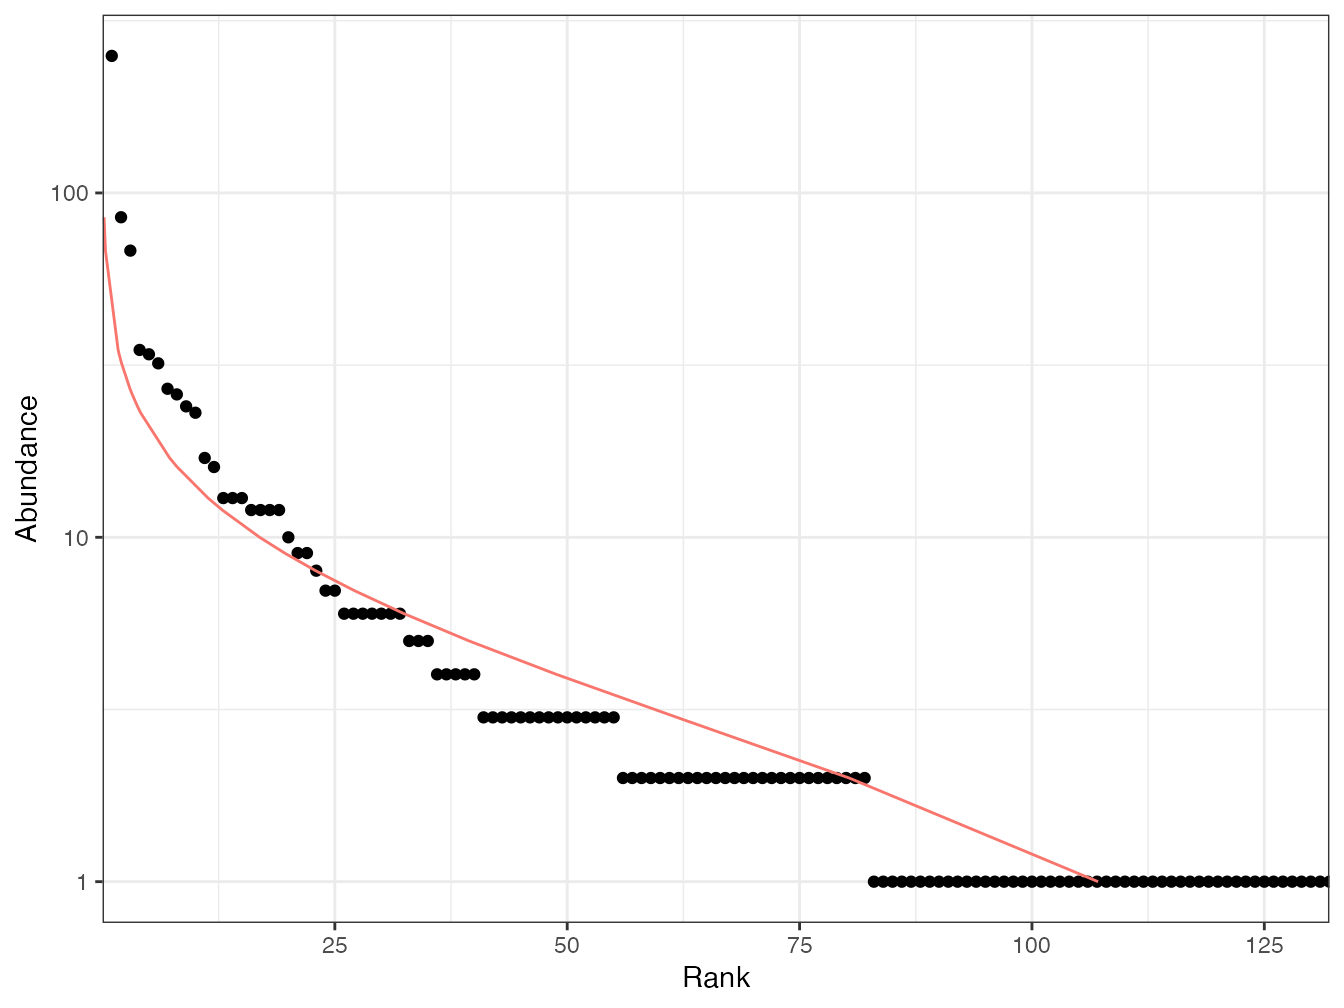
\includegraphics[width=0.8\linewidth]{MesuresBD_files/figure-latex/BiaisJack1Fig-1} 

}

\caption{Echantillon de 1000 individus tiré dans une communauté log-normale.}\label{fig:BiaisJack1Fig}
\end{SCfigure}

\normalsize

Il est possible de vérifier que l'espérance du nombre d'espèces non observées correspond bien à la moyenne des observations.

\scriptsize

\begin{Shaded}
\begin{Highlighting}[]
\CommentTok{# Espérance des espèces non vues}
\NormalTok{E0 <-}\StringTok{ }\NormalTok{(}\DecValTok{1} \OperatorTok{-}\StringTok{ }\NormalTok{Ps)}\OperatorTok{^}\NormalTok{N}
\NormalTok{(f0 <-}\StringTok{ }\KeywordTok{sum}\NormalTok{(E0))}
\end{Highlighting}
\end{Shaded}

\begin{verbatim}
## [1] 179.4575
\end{verbatim}

\begin{Shaded}
\begin{Highlighting}[]
\CommentTok{# Tirage de 1000 échantillons, nombre moyen d'espèces}
\CommentTok{# observées}
\NormalTok{(Sn <-}\StringTok{ }\KeywordTok{mean}\NormalTok{(}\KeywordTok{colSums}\NormalTok{(}\KeywordTok{rmultinom}\NormalTok{(}\DecValTok{1000}\NormalTok{, N, Ps) }\OperatorTok{>}\StringTok{ }\DecValTok{0}\NormalTok{)))}
\end{Highlighting}
\end{Shaded}

\begin{verbatim}
## [1] 120.565
\end{verbatim}

\begin{Shaded}
\begin{Highlighting}[]
\CommentTok{# Vérification: nombre d'espèces observées en moyenne et non}
\CommentTok{# observées}
\NormalTok{Sn }\OperatorTok{+}\StringTok{ }\NormalTok{f0}
\end{Highlighting}
\end{Shaded}

\begin{verbatim}
## [1] 300.0225
\end{verbatim}

\begin{Shaded}
\begin{Highlighting}[]
\CommentTok{# Nombre total d'espèces dans la communauté}
\NormalTok{(S <-}\StringTok{ }\KeywordTok{length}\NormalTok{(Ps))}
\end{Highlighting}
\end{Shaded}

\begin{verbatim}
## [1] 300
\end{verbatim}

\normalsize

Le nombre d'espèces non observées peut être écrit sous la forme d'une série de puissances négatives de \(n\), comme le prévoit le jackknife, entre deux valeurs de \(n\) fixées.

\scriptsize

\begin{Shaded}
\begin{Highlighting}[]
\CommentTok{# Echantillonnage de 500 à 5000 individus}
\NormalTok{n.seq <-}\StringTok{ }\DecValTok{500}\OperatorTok{:}\DecValTok{5000}
\CommentTok{# Calcul du nombre d'espèces non observées}
\NormalTok{Bias <-}\StringTok{ }\KeywordTok{sapply}\NormalTok{(n.seq, }\ControlFlowTok{function}\NormalTok{(n) }\KeywordTok{sum}\NormalTok{((}\DecValTok{1} \OperatorTok{-}\StringTok{ }\NormalTok{Ps)}\OperatorTok{^}\NormalTok{n))}
\end{Highlighting}
\end{Shaded}

\normalsize

Le nombre d'espèces non observées, qui est le biais de l'estimateur de la richesse, est présenté en figure \ref{fig:BiaisJack3Fig}.

Code de la figure \ref{fig:BiaisJack3Fig}:

\scriptsize

\begin{Shaded}
\begin{Highlighting}[]
\KeywordTok{ggplot}\NormalTok{(}\KeywordTok{data.frame}\NormalTok{(}\DataTypeTok{n=}\NormalTok{n.seq, }\DataTypeTok{Biais=}\NormalTok{Bias, }\DataTypeTok{lm1=}\KeywordTok{predict}\NormalTok{(lm1), }
        \DataTypeTok{lm2=}\KeywordTok{predict}\NormalTok{(lm2), }\DataTypeTok{lm4=}\KeywordTok{predict}\NormalTok{(lm4)), }\KeywordTok{aes}\NormalTok{(}\DataTypeTok{x=}\NormalTok{n)) }\OperatorTok{+}
\StringTok{  }\KeywordTok{geom_line}\NormalTok{(}\KeywordTok{aes}\NormalTok{(}\DataTypeTok{y=}\NormalTok{Biais), }\DataTypeTok{col=}\StringTok{"black"}\NormalTok{, }\DataTypeTok{lty=}\DecValTok{1}\NormalTok{) }\OperatorTok{+}
\StringTok{  }\KeywordTok{geom_line}\NormalTok{(}\KeywordTok{aes}\NormalTok{(}\DataTypeTok{y=}\NormalTok{lm1), }\DataTypeTok{col=}\StringTok{"red"}\NormalTok{, }\DataTypeTok{lty=}\DecValTok{2}\NormalTok{) }\OperatorTok{+}
\StringTok{  }\KeywordTok{geom_line}\NormalTok{(}\KeywordTok{aes}\NormalTok{(}\DataTypeTok{y=}\NormalTok{lm2), }\DataTypeTok{col=}\StringTok{"orange"}\NormalTok{, }\DataTypeTok{lty=}\DecValTok{3}\NormalTok{) }\OperatorTok{+}
\StringTok{  }\KeywordTok{geom_line}\NormalTok{(}\KeywordTok{aes}\NormalTok{(}\DataTypeTok{y=}\NormalTok{lm4), }\DataTypeTok{col=}\StringTok{"blue"}\NormalTok{, }\DataTypeTok{lty=}\DecValTok{4}\NormalTok{) }\OperatorTok{+}
\StringTok{  }\KeywordTok{coord_cartesian}\NormalTok{(}\DataTypeTok{ylim =} \KeywordTok{c}\NormalTok{(}\DecValTok{0}\NormalTok{, }\DecValTok{250}\NormalTok{))}
\end{Highlighting}
\end{Shaded}

\normalsize

La courbe peut être approchée par une série de puissances négatives de \(n\) dont quelques termes sont présentés sur la figure.

\scriptsize

\begin{Shaded}
\begin{Highlighting}[]
\CommentTok{# Ordre 1}
\NormalTok{lm1 <-}\StringTok{ }\KeywordTok{lm}\NormalTok{(Bias }\OperatorTok{~}\StringTok{ }\DecValTok{0} \OperatorTok{+}\KeywordTok{I}\NormalTok{(}\DecValTok{1}\OperatorTok{/}\NormalTok{n.seq))}
\CommentTok{# Ordre 2}
\NormalTok{lm2 <-}\StringTok{ }\KeywordTok{lm}\NormalTok{(Bias }\OperatorTok{~}\StringTok{ }\DecValTok{0} \OperatorTok{+}\KeywordTok{I}\NormalTok{(}\DecValTok{1}\OperatorTok{/}\NormalTok{n.seq) }\OperatorTok{+}\StringTok{ }\KeywordTok{I}\NormalTok{(}\DecValTok{1}\OperatorTok{/}\NormalTok{n.seq}\OperatorTok{^}\DecValTok{2}\NormalTok{))}
\CommentTok{# Ordre 4}
\KeywordTok{summary}\NormalTok{(lm4 <-}\StringTok{ }\KeywordTok{lm}\NormalTok{(Bias }\OperatorTok{~}\StringTok{ }\DecValTok{0} \OperatorTok{+}\KeywordTok{I}\NormalTok{(}\DecValTok{1}\OperatorTok{/}\NormalTok{n.seq) }\OperatorTok{+}\StringTok{ }\KeywordTok{I}\NormalTok{(}\DecValTok{1}\OperatorTok{/}\NormalTok{n.seq}\OperatorTok{^}\DecValTok{2}\NormalTok{) }
                  \OperatorTok{+}\StringTok{ }\KeywordTok{I}\NormalTok{(}\DecValTok{1}\OperatorTok{/}\NormalTok{n.seq}\OperatorTok{^}\DecValTok{3}\NormalTok{) }\OperatorTok{+}\StringTok{ }\KeywordTok{I}\NormalTok{(}\DecValTok{1}\OperatorTok{/}\NormalTok{n.seq}\OperatorTok{^}\DecValTok{4}\NormalTok{)))}
\end{Highlighting}
\end{Shaded}

\begin{verbatim}
## 
## Call:
## lm(formula = Bias ~ 0 + I(1/n.seq) + I(1/n.seq^2) + I(1/n.seq^3) + 
##     I(1/n.seq^4))
## 
## Residuals:
##     Min      1Q  Median      3Q     Max 
## -8.4563 -3.0845  0.1785  3.6379 21.2393 
## 
## Coefficients:
##                Estimate Std. Error t value Pr(>|t|)    
## I(1/n.seq)    5.787e+05  7.548e+02   766.7   <2e-16 ***
## I(1/n.seq^2) -7.975e+08  2.652e+06  -300.8   <2e-16 ***
## I(1/n.seq^3)  5.071e+11  2.669e+09   190.0   <2e-16 ***
## I(1/n.seq^4) -1.145e+14  8.003e+11  -143.1   <2e-16 ***
## ---
## Signif. codes:  0 '***' 0.001 '**' 0.01 '*' 0.05 '.' 0.1 ' ' 1
## 
## Residual standard error: 3.757 on 4497 degrees of freedom
## Multiple R-squared:  0.9992, Adjusted R-squared:  0.9992 
## F-statistic: 1.482e+06 on 4 and 4497 DF,  p-value: < 2.2e-16
\end{verbatim}

\normalsize



\scriptsize

\begin{SCfigure}

{\centering 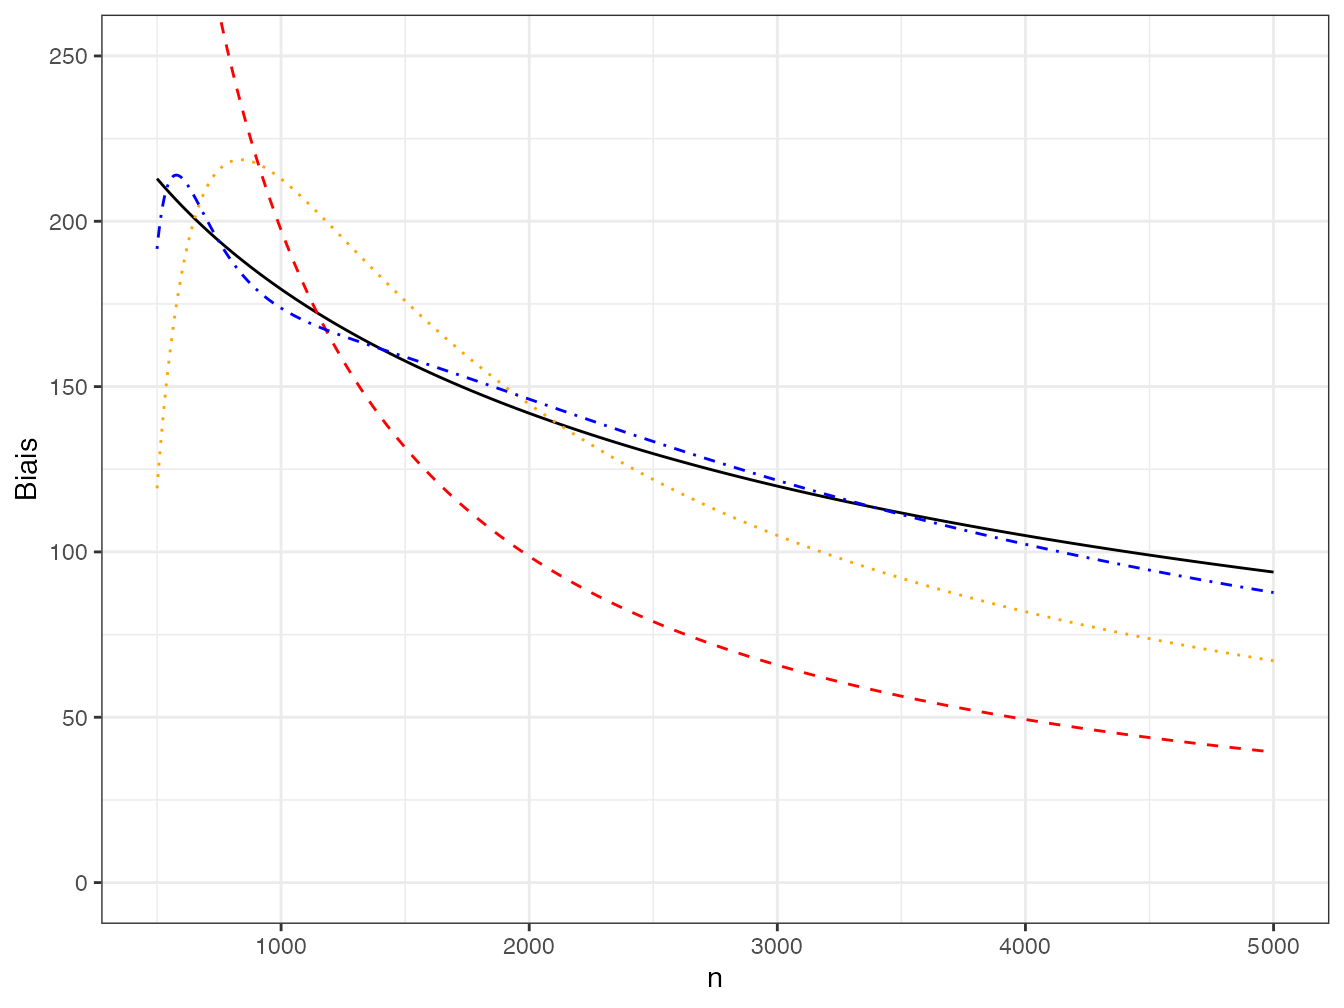
\includegraphics[width=0.8\linewidth]{MesuresBD_files/figure-latex/BiaisJack3Fig-1} 

}

\caption{Nombre d'espèces non obervées dans un échantillon de taille croissante et sa décomposition en séries de puissances négatives de \(n\). Le nombre d'espèces non observées est représenté par la courbe continue noire. Les séries de puissances négatives d'ordre 1 (courbe rouge), 2 (courbe orange) et 4 (courbe bleue) sont représentées en pointillés. Les courbes d'ordre 6 et plus sont confondues avec la courbe noire.}\label{fig:BiaisJack3Fig}
\end{SCfigure}

\normalsize

L'ajustement est possible pour des valeurs de \(n\) différentes mais les coefficients \(a_i\) sont alors différents: la forme du biais n'est valide que pour une gamme de valeurs de \(n\) fixée.

\textcite{Beguinot2016} apporte un autre argument important en faveur du jackknife.
À condition que \(n\) soit suffisamment grand, l'estimateur du nombre d'espèces non observées est une fonction linéaire du nombre d'espèces observées \(\nu\) fois: \(s^{n}_{1}\) pour le jackknife 1, \(2 s^{n}_{1} - s^{n}_{2}\) pour le jackknife 2 et ainsi de suite pour les ordres suivants, contrairement à l'estimateur de Chao.
Grâce à cette propriété, l'estimateur du jackknife est additif quand plusieurs groupes d'espèces disjoints sont pris en compte: l'estimation du nombre d'espèces de papillons et de scarabées inventoriées ensemble est égale à la somme des estimations des deux groupes inventoriés séparément.
Ce n'est pas le cas pour l'estimateur de Chao.

L'estimateur du jackknife est très utilisé parce qu'il est efficace en pratique, notamment parce que son ordre peut être adapté aux données.

\hypertarget{lestimateur-du-bootstrap}{%
\subsubsection{L'estimateur du bootstrap}\label{lestimateur-du-bootstrap}}

L'estimateur du bootstrap \autocite{Smith1984} est
\begin{equation} 
  \label{eq:Smith1984}
  \hat{S}_\mathit{b} = {s^{n}_{\ne 0}} + \sum_s{(1-p_s)^n}.
\end{equation}

Il est peu utilisé parce que le jackknife est plus performant \autocite{Colwell1994}.

\hypertarget{calcul}{%
\subsubsection{Calcul}\label{calcul}}

Ces estimateurs peuvent être calculés de façon relativement simple à l'aide du logiciel SPADE, dans sa version pour R \autocite{Chao2016c}.
Le guide de l'utilisateur présente quelques estimateurs supplémentaires et des directives pour choisir.
Il est conseillé d'utiliser Chao1 pour une estimation minimale, et ACE pour une estimation moins biaisée de la richesse.

Les intervalles de confiance de chaque estimateur sont calculés par bootstrap: même quand la variance d'un estimateur est connue, sa loi ne l'est généralement pas, et le calcul analytique de l'intervalle de confiance n'est pas possible.

Les estimateurs et leurs intervalles de confiance peuvent également être calculés avec le package \emph{vegan} qui dispose pour cela de deux fonctions: \texttt{specpool} et \texttt{estimateR}.

\texttt{specpool} est basé sur les incidences des espèces dans un ensemble de sites d'observation et donne une estimation unique de la richesse selon les méthodes Chao2, jackknife (ordre 1 et 2) et bootstrap.
L'écart-type de l'estimateur est également fourni par la fonction, sauf pour le jackknife d'ordre 2.

\texttt{estimateR} est basé sur les abondances des espèces et retourne un estimateur de la richesse spécifique par site et non global comme \texttt{specpool}.

\hypertarget{exemple}{%
\subsubsection{Exemple}\label{exemple}}

On utilise les données de Barro Colorado Island (BCI).
La parcelle a été divisée en carrés de 1~ha.
Le tableau d'entrée est un \texttt{dataframe} contenant, pour chaque espèce d'arbres (\(\mathit{DBH}\ge\) 10~cm), ses effectifs par carré.

On charge le tableau de données:

\scriptsize

\begin{Shaded}
\begin{Highlighting}[]
\KeywordTok{library}\NormalTok{(}\StringTok{"vegan"}\NormalTok{)}
\KeywordTok{data}\NormalTok{(BCI)}
\end{Highlighting}
\end{Shaded}

\normalsize

On utilise la fonction \texttt{estimateR} pour calculer la richesse des deux premiers carrés:

\scriptsize

\begin{Shaded}
\begin{Highlighting}[]
\KeywordTok{estimateR}\NormalTok{(BCI[}\DecValTok{1}\OperatorTok{:}\DecValTok{2}\NormalTok{, ])}
\end{Highlighting}
\end{Shaded}

\begin{verbatim}
##                   1          2
## S.obs     93.000000  84.000000
## S.chao1  117.473684 117.214286
## se.chao1  11.583785  15.918953
## S.ACE    122.848959 117.317307
## se.ACE     5.736054   5.571998
\end{verbatim}

\normalsize

Le package \emph{SPECIES} \autocite{Wang2011} permet de calculer les estimateurs jackknife d'ordre supérieur à 2 et surtout choisit l'ordre qui fournit le meilleur compromis entre biais et variance.

Comparaison des fonctions sur l'ensemble du dispositif BCI (\(s^{n}_{\ne 0}=225\), \(s_{1}=19\)):

\scriptsize

\begin{Shaded}
\begin{Highlighting}[]
\KeywordTok{specpool}\NormalTok{(BCI)}
\end{Highlighting}
\end{Shaded}

\begin{verbatim}
##     Species     chao chao.se  jack1 jack1.se    jack2     boot  boot.se  n
## All     225 236.3732 6.54361 245.58 5.650522 247.8722 235.6862 3.468888 50
\end{verbatim}

\begin{Shaded}
\begin{Highlighting}[]
\KeywordTok{library}\NormalTok{(}\StringTok{"SPECIES"}\NormalTok{)}
\CommentTok{# Distribution du nombre d'espèces (vecteur: }
\CommentTok{# noms = nombre d'individus}
\CommentTok{# valeurs = nombres d'espèces ayant ce nombre d'individus)}
\NormalTok{Ns <-}\StringTok{ }\KeywordTok{colSums}\NormalTok{(BCI)}
\CommentTok{# Mise au format requis (matrice:}
\CommentTok{# colonne 1 = nombre d'individus}
\CommentTok{# colonne 2 = nombres d'espèces ayant ce nombre d'individus)}
\CommentTok{# par la fonction AbdFreqCount dans entropart}
\KeywordTok{jackknife}\NormalTok{(}\KeywordTok{AbdFreqCount}\NormalTok{(Ns))}
\end{Highlighting}
\end{Shaded}

\begin{verbatim}
## 
## Your specified order is larger than that determined by the test, 
## Therefore the order from the test is used.
\end{verbatim}

\begin{verbatim}
## $JackknifeOrder
## [1] 1
## 
## $Nhat
## [1] 244
## 
## $SE
## [1] 6.164414
## 
## $CI
##       lb  ub
## [1,] 232 256
\end{verbatim}

\normalsize

Comparaison avec la valeur de l'équation \eqref{eq:Jack1}:

\scriptsize

\begin{Shaded}
\begin{Highlighting}[]
\CommentTok{# Nombre d'espèces par efffectif observé}
\NormalTok{DistNs <-}\StringTok{ }\KeywordTok{tapply}\NormalTok{(Ns, Ns, length)}
\CommentTok{# Calcul direct de Jack1}
\KeywordTok{sum}\NormalTok{(DistNs) }\OperatorTok{+}\StringTok{ }\NormalTok{DistNs[}\DecValTok{1}\NormalTok{] }\OperatorTok{*}\StringTok{ }\NormalTok{(}\KeywordTok{sum}\NormalTok{(BCI) }\OperatorTok{-}\StringTok{ }\DecValTok{1}\NormalTok{)}\OperatorTok{/}\KeywordTok{sum}\NormalTok{(BCI)}
\end{Highlighting}
\end{Shaded}

\begin{verbatim}
##        1 
## 243.9991
\end{verbatim}

\normalsize

La valeur du jackknife 1 fournie par \texttt{specpool} est fausse.
La fonction \texttt{jackknife} de \emph{SPECIES} donne le bon résultat, avec un intervalle de confiance calculé en supposant que la distribution est normale (\(\pm\) 1,96 écart-type au seuil de 95\%).

L'estimateur du bootstrap est calculable simplement:

\scriptsize

\begin{Shaded}
\begin{Highlighting}[]
\NormalTok{N <-}\StringTok{ }\KeywordTok{sum}\NormalTok{(Ns)}
\NormalTok{Ps <-}\StringTok{ }\NormalTok{Ns}\OperatorTok{/}\NormalTok{N}
\KeywordTok{length}\NormalTok{(Ps) }\OperatorTok{+}\StringTok{ }\KeywordTok{sum}\NormalTok{((}\DecValTok{1} \OperatorTok{-}\StringTok{ }\NormalTok{Ps)}\OperatorTok{^}\NormalTok{N)}
\end{Highlighting}
\end{Shaded}

\begin{verbatim}
## [1] 234.3517
\end{verbatim}

\normalsize

\hypertarget{sec:ChoixEstimateur}{%
\subsubsection{Choix de l'estimateur}\label{sec:ChoixEstimateur}}

Des tests poussés ont été menés par \textcite{Brose2003} pour permettre le choix du meilleur estimateur de la richesse en fonction de la complétude de l'échantillonnage \(s^{n}_{\ne 0}/{S}\).
Les auteurs appellent cette proportion couverture (\emph{coverage}).
Le terme \emph{completeness} a été proposé par \textcite{Beck2010} pour éviter la confusion avec le taux de couverture défini par Good (vu en section \ref{sec:Couverture}).
La complétude est inférieure à la couverture: toutes les espèces ont le même poids alors que les espèces manquantes sont plus rares et pénalisent moins le taux de couverture.



\scriptsize

\begin{SCfigure}

{\centering 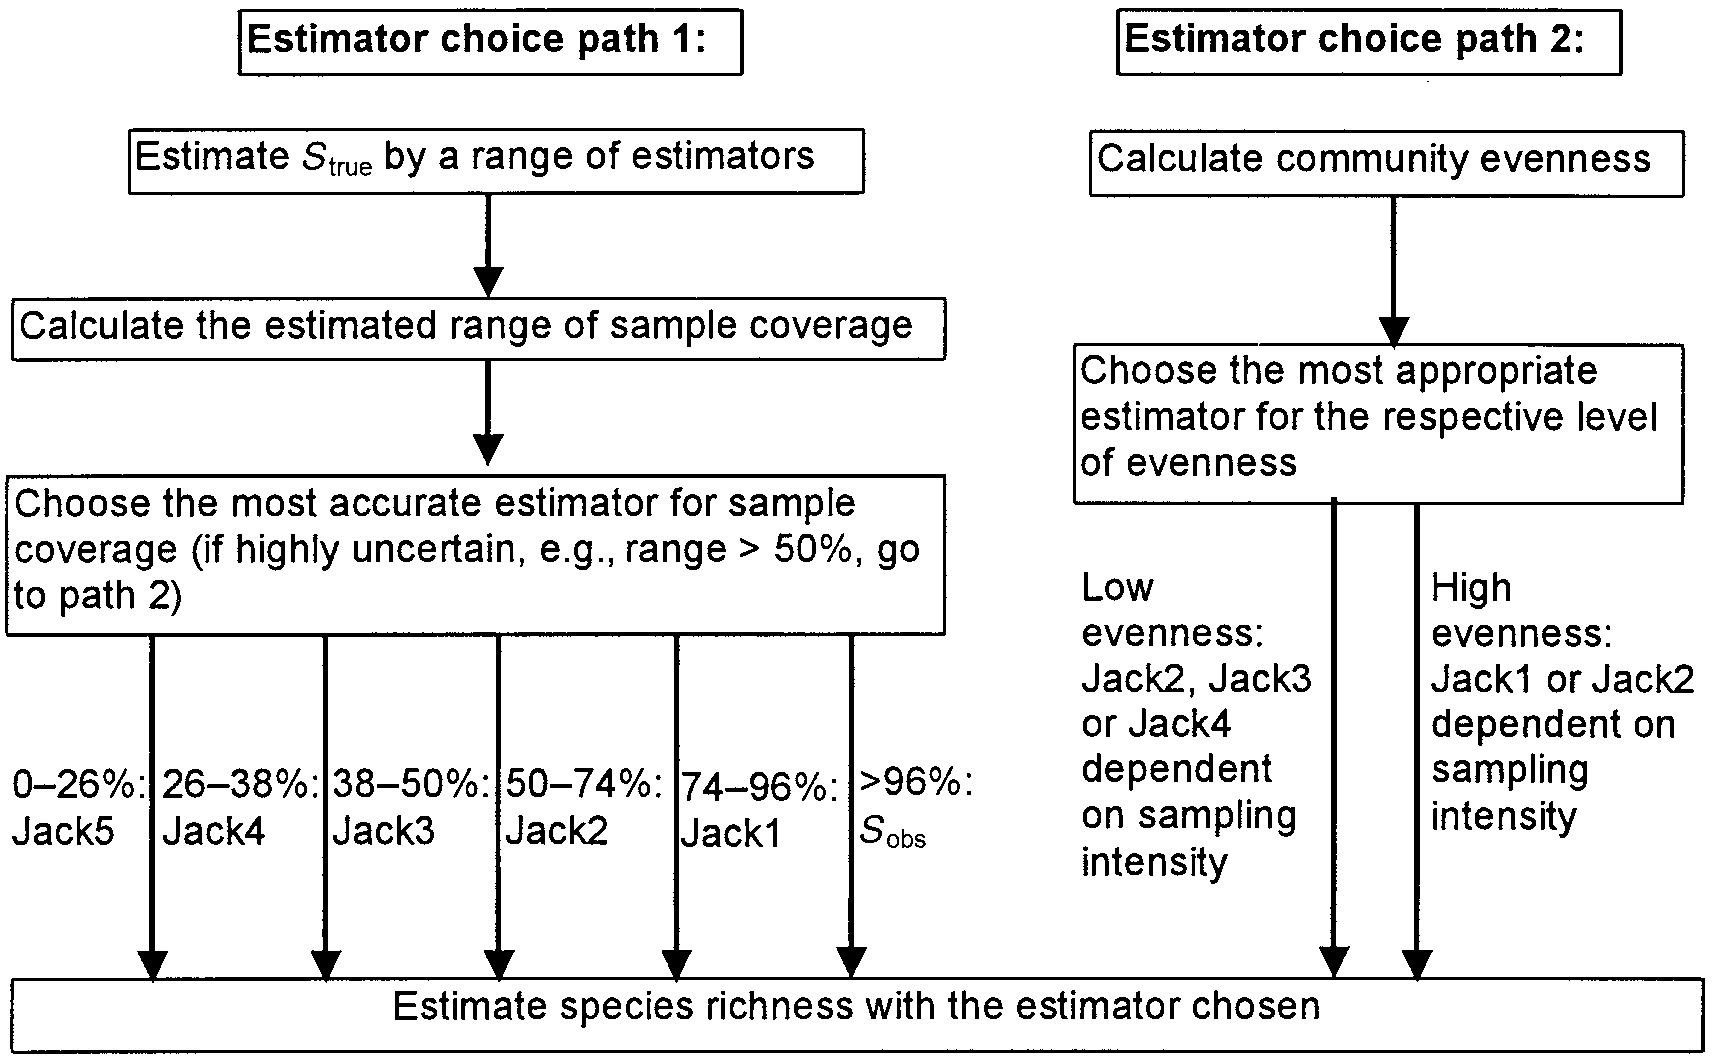
\includegraphics[width=0.8\linewidth]{images/Brose2003} 

}

\caption{Arbre de décision du meilleur estimateur du nombre d'espèces.}\label{fig:Brose2003}
\end{SCfigure}

\normalsize

Dans tous les cas, les estimateurs jackknife sont les meilleurs.
L'arbre de décision est en figure \ref{fig:Brose2003} \autocite[fig.~6]{Brose2003}.
Le choix dépend principalement de la complétude (\emph{coverage} sur la figure).
Une première estimation est nécessaire par plusieurs estimateurs.
Si les résultats sont cohérents, choisir un estimateur jackknife d'ordre d'autant plus faible que la complétude est grande.
Au-delà de 96\%, le nombre d'espèces observé est plus performant parce que les jackknifes surestiment \(S\).
S'ils sont incohérents (intervalle des estimations supérieur à 50\% de leur moyenne), le critère majeur est l'équitabilité (voir section \ref{sec:Equitabilite}).
Si elle est faible (de l'ordre de 0,5-0,6), les estimateurs jackknife 2 à 4 sont performants, l'ordre diminuant avec l'intensité d'échantillonnage (forte: 10\%, faible: 0,5\% de la communauté).
Pour une forte équitabilité (0,8-0,9), on préférera jackknife 1 ou 2.

Pour BCI, le nombre d'espèces estimé par jackknife 1 est 244.
La complétude est \({225}/{244}=92\%\), dans le domaine de validité du jackknife 1 (74\% à 96\%) qui est donc le bon estimateur.

La parcelle 6 de Paracou nécessite l'estimateur jackknife 2:

\scriptsize

\begin{Shaded}
\begin{Highlighting}[]
\KeywordTok{library}\NormalTok{(}\StringTok{"SpatDiv"}\NormalTok{)}
\KeywordTok{jackknife}\NormalTok{(}\KeywordTok{AbdFreqCount}\NormalTok{(}\KeywordTok{as.AbdVector}\NormalTok{(Paracou6)))}
\end{Highlighting}
\end{Shaded}

\begin{verbatim}
## 
## Your specified order is larger than that determined by the test, 
## Therefore the order from the test is used.
\end{verbatim}

\begin{verbatim}
## $JackknifeOrder
## [1] 2
## 
## $Nhat
## [1] 471
## 
## $SE
## [1] 24.24871
## 
## $CI
##       lb  ub
## [1,] 423 519
\end{verbatim}

\begin{Shaded}
\begin{Highlighting}[]
\CommentTok{# Complétude}
\KeywordTok{as.numeric}\NormalTok{(}\KeywordTok{Richness}\NormalTok{(Paracou6, }\DataTypeTok{Correction =} \StringTok{"None"}\NormalTok{)}\OperatorTok{/}\KeywordTok{Richness}\NormalTok{(Paracou6, }
    \DataTypeTok{Correction =} \StringTok{"Jackknife"}\NormalTok{))}
\end{Highlighting}
\end{Shaded}

\begin{verbatim}
## [1] 0.7091295
\end{verbatim}

\normalsize

\textcite{Chiu2014a}, à partir d'autres simulations, préfèrent l'utilisation de l'estimateur \emph{iChao1}.
Quand l'échantillonnage est suffisant, les estimateurs de Chao ont l'avantage de posséder une base théorique solide et de fournir une borne inférieure du nombre d'espèces possible.
Dans ce cas, les estimations du jackknife d'ordre 1 sont cohérentes avec celles de Chao.
En revanche, quand l'échantillonnage est insuffisant, l'estimateur jackknife d'ordre supérieur à 1 permet de réduire le biais d'estimation, au prix d'une variance accrue \autocite{Marcon2015a}.

Enfin, Beguinot \autocite*{Beguinot2015a,Beguinot2016} suggère d'utiliser en règle générale le jacknife 2 (mais ne traite pas les cas dans lesquels l'échantillonnage est trop faible pour justifier un ordre supérieur) tant que le nombre de singletons est supérieur à \(2-\sqrt(2) \approx 0,6\) fois le nombre de doubletons.
Le ratio des singletons sur les doubletons diminue quand l'échantillonnage approche de l'exhaustivité.
Quand le seuil de 0,6 est dépassé, la valeur de l'estimateur de Chao devient supérieur au jacknife 2 et doit être utilisé.
Ce seuil est cohérent avec les règles de \textcite{Brose2003}.

\hypertarget{sec:Extrapol}{%
\subsubsection{Prédiction de la richesse d'un nouvel échantillon}\label{sec:Extrapol}}

La prédiction du nombre d'espèces \(\hat{S'}\) découvert dans une nouvelle placette d'un habitat dans lequel on a déjà échantillonné est une question importante, par exemple pour évaluer le nombre d'espèces préservées dans le cadre d'une mise en réserve, ou évaluer le nombre d'espèces perdues en réduisant la surface d'une forêt.

\textcite{Shen2003} proposent un estimateur et le confrontent avec succès à des estimateurs antérieurs.
On note \(\hat{S}^{n}_{0}\) l'estimateur du nombre d'espèces non observées dans le premier échantillon, et \(\hat{C}\) l'estimateur de son taux de couverture.
L'estimateur du nombre d'espèces du nouvel échantillon de \(n'\) individus est

\begin{equation}
  \hat{S'} = \hat{S}^{n}_{0} \left[1-{\left(1-\frac{1-\hat{C}}{\hat{S}^{n}_{0}}\right)}^{n'}\right].
\end{equation}

\(\hat{S}^{n}_{0}\) est obtenu par la différence entre les nombres d'espèces estimé et observé: \(\hat{S}^{n}_{0}=\hat{S}-s^{n}_{\ne 0}\).

Exemple de BCI, suite: combien de nouvelles espèces seront découvertes en échantillonnant plus?

\scriptsize

\begin{Shaded}
\begin{Highlighting}[]
\CommentTok{# Espèces non observées}
\NormalTok{(NonObs <-}\StringTok{ }\KeywordTok{jackknife}\NormalTok{(}\KeywordTok{AbdFreqCount}\NormalTok{(Ns))}\OperatorTok{$}\NormalTok{Nhat }\OperatorTok{-}\StringTok{ }\KeywordTok{length}\NormalTok{(Ns))}
\end{Highlighting}
\end{Shaded}

\begin{verbatim}
## 
## Your specified order is larger than that determined by the test, 
## Therefore the order from the test is used.
\end{verbatim}

\begin{verbatim}
## [1] 19
\end{verbatim}

\begin{Shaded}
\begin{Highlighting}[]
\CommentTok{# Taux de couverture}
\NormalTok{(C <-}\StringTok{ }\KeywordTok{Coverage}\NormalTok{(Ns))}
\end{Highlighting}
\end{Shaded}

\begin{verbatim}
## ZhangHuang 
##  0.9991146
\end{verbatim}

\normalsize



\scriptsize

\begin{SCfigure}

{\centering 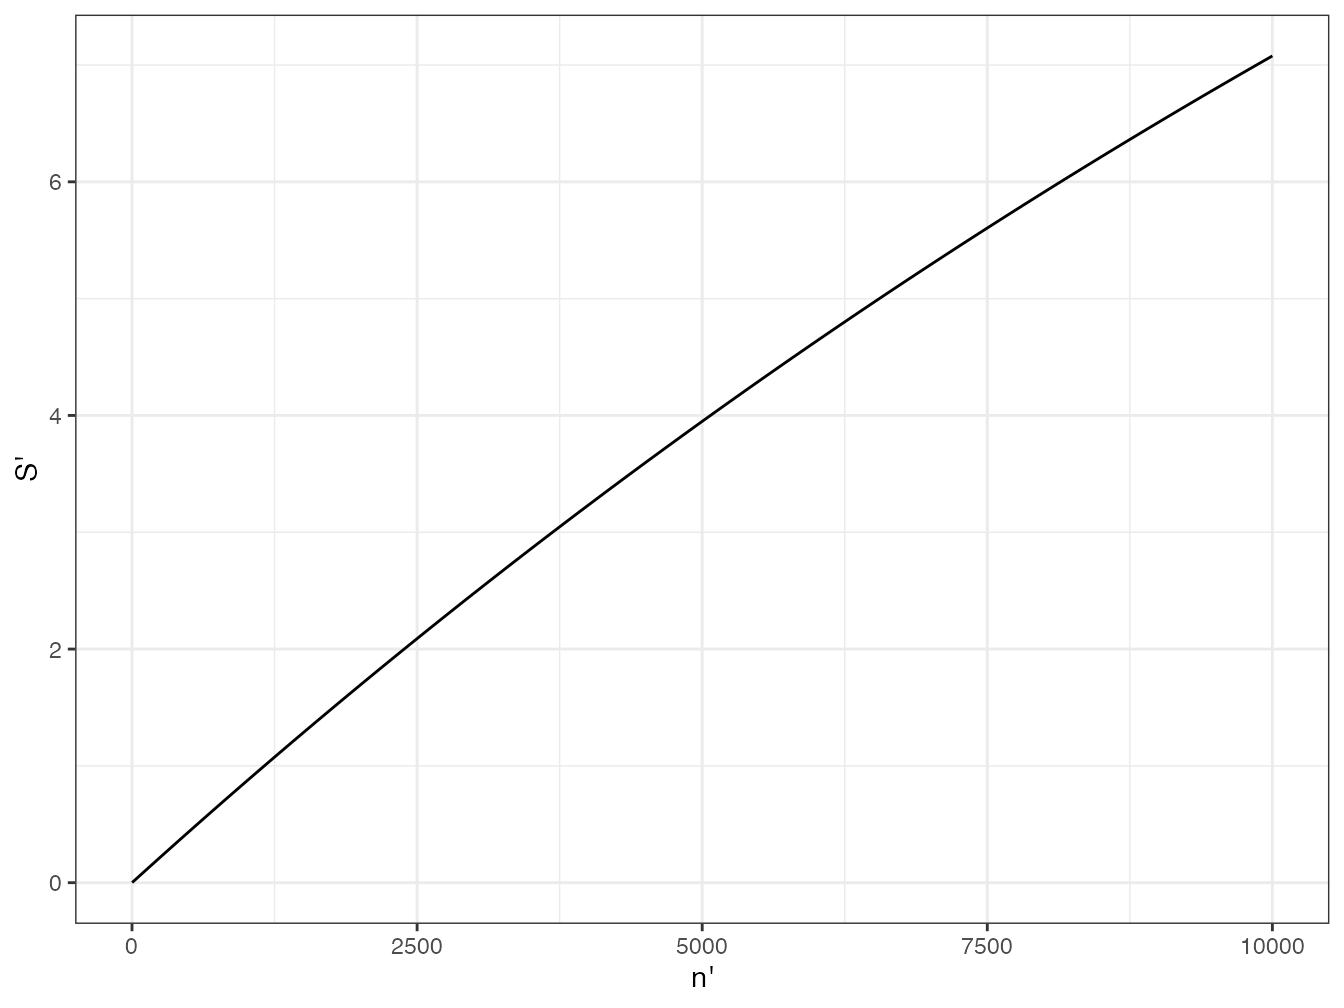
\includegraphics[width=0.8\linewidth]{MesuresBD_files/figure-latex/NonObsNFig-1} 

}

\caption{Nombre de nouvelles espèces découvertes en fonction de l'effort d'échantillonnage supplémentaire (données de BCI). Seulement 7 nouvelles espèces seront observées en échantillonnant 10000 arbres supplémentaires (environ 25 ha en plus des 50 ha de la parcelle qui contiennent 225 espèces).}\label{fig:NonObsNFig}
\end{SCfigure}

\normalsize

Le taux de couverture de l'inventaire de BCI est très proche de 100\%, donc peu de nouvelles espèces seront découvertes en augmentant l'effort d'échantillonnage.
La courbe obtenue est en figure \ref{fig:NonObsNFig}.

Le code R nécessaire pour réaliser la figure est:

\scriptsize

\begin{Shaded}
\begin{Highlighting}[]
\CommentTok{# Nouvelles espèces en fonction du nombre de nouveaux individus}
\NormalTok{Sprime <-}\StringTok{ }\ControlFlowTok{function}\NormalTok{(Nprime) NonObs }\OperatorTok{*}\StringTok{ }\NormalTok{(}\DecValTok{1} \OperatorTok{-}\StringTok{ }\NormalTok{(}\DecValTok{1} \OperatorTok{-}\StringTok{ }\NormalTok{(}\DecValTok{1} \OperatorTok{-}\StringTok{ }\NormalTok{C)}\OperatorTok{/}\NormalTok{NonObs)}\OperatorTok{^}\NormalTok{Nprime)}
\KeywordTok{ggplot}\NormalTok{(}\KeywordTok{data.frame}\NormalTok{(}\DataTypeTok{x =} \KeywordTok{c}\NormalTok{(}\DecValTok{1}\NormalTok{, }\DecValTok{10000}\NormalTok{)), }\KeywordTok{aes}\NormalTok{(x)) }\OperatorTok{+}\StringTok{ }
\StringTok{  }\KeywordTok{stat_function}\NormalTok{(}\DataTypeTok{fun =}\NormalTok{ Sprime) }\OperatorTok{+}
\StringTok{  }\KeywordTok{labs}\NormalTok{(}\DataTypeTok{x =} \StringTok{"n'"}\NormalTok{, }\DataTypeTok{y =} \StringTok{"S'"}\NormalTok{)}
\end{Highlighting}
\end{Shaded}

\normalsize

La question de l'extrapolation de la richesse est traitée plus en détail dans les sections \ref{sec:RarExtrapol} et \ref{sec:Extrapolation}.

\hypertarget{infuxe9rence-du-nombre-despuxe8ces-uxe0-partir-de-la-sad}{%
\subsection{Inférence du nombre d'espèces à partir de la SAD}\label{infuxe9rence-du-nombre-despuxe8ces-uxe0-partir-de-la-sad}}

\hypertarget{distribution-de-preston}{%
\subsubsection{Distribution de Preston}\label{distribution-de-preston}}

\textcite{Preston1948} fournit dès l'introduction de son modèle log-normal une technique d'estimation du nombre total d'espèces par la célèbre méthode des octaves.
Elle est disponible dans le package \emph{vegan}:

\scriptsize

\begin{Shaded}
\begin{Highlighting}[]
\KeywordTok{veiledspec}\NormalTok{(}\KeywordTok{colSums}\NormalTok{(BCI))}
\end{Highlighting}
\end{Shaded}

\begin{verbatim}
## Extrapolated     Observed       Veiled 
##    235.40577    225.00000     10.40577
\end{verbatim}

\normalsize

L'ajustement direct du modèle aux données, sans regroupement par octaves \autocite{Williamson2005}, est également possible (figure \ref{fig:PrestonSansOFig}):

\scriptsize

\begin{Shaded}
\begin{Highlighting}[]
\NormalTok{mod.ll <-}\StringTok{ }\KeywordTok{prestondistr}\NormalTok{(}\KeywordTok{colSums}\NormalTok{(BCI))}
\KeywordTok{veiledspec}\NormalTok{(mod.ll)}
\end{Highlighting}
\end{Shaded}

\begin{verbatim}
## Extrapolated     Observed       Veiled 
##   230.931018   225.000000     5.931018
\end{verbatim}

\normalsize



\scriptsize

\begin{SCfigure}

{\centering 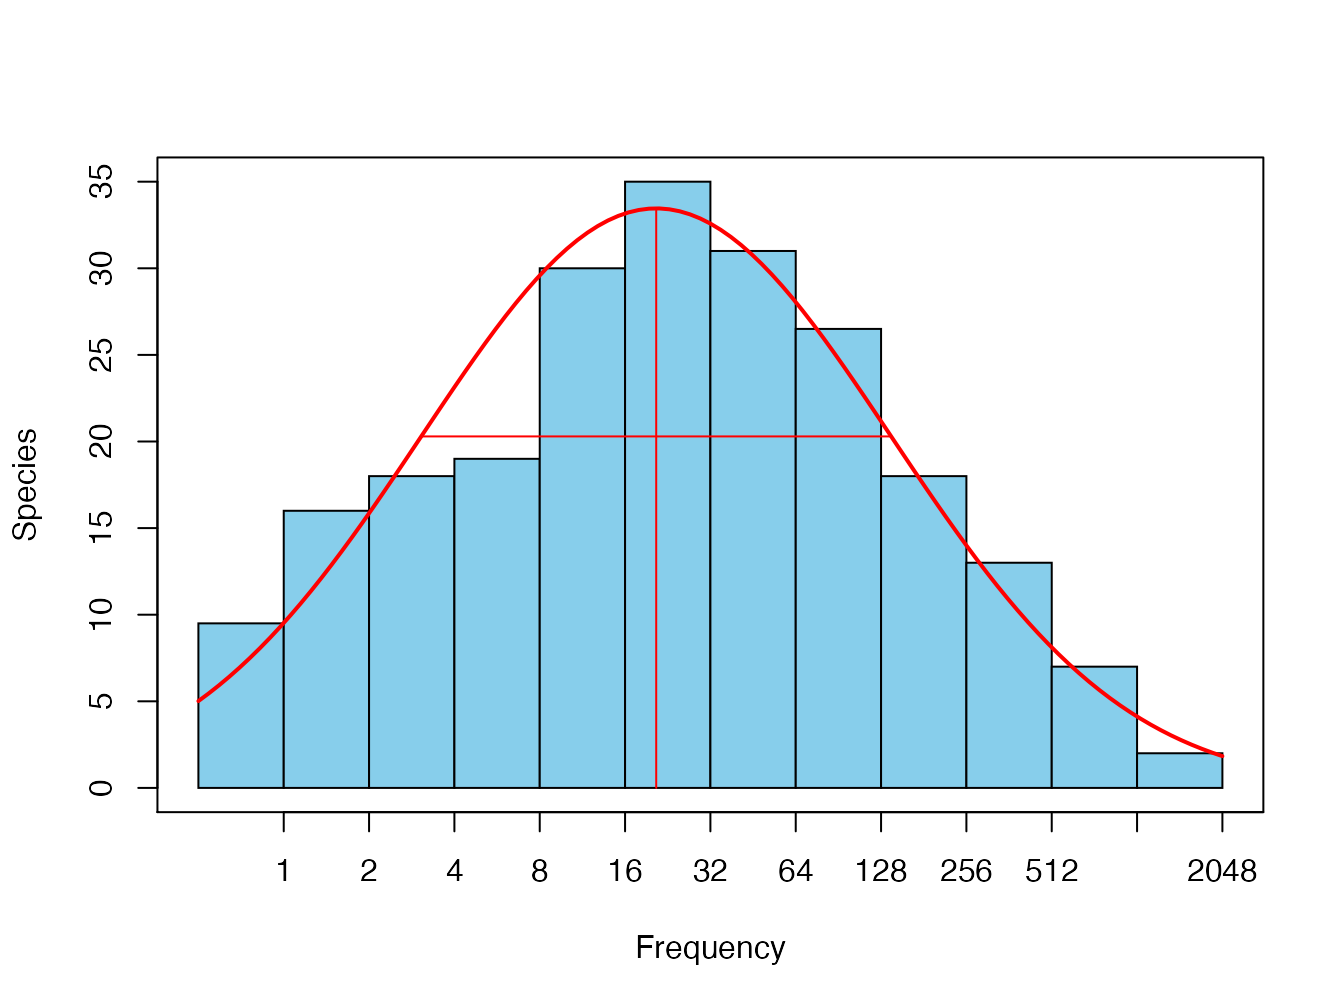
\includegraphics[width=0.8\linewidth]{MesuresBD_files/figure-latex/PrestonSansOFig-1} 

}

\caption{Ajustement du modèle de Preston aux données de BCI.}\label{fig:PrestonSansOFig}
\end{SCfigure}

\normalsize

Le code R nécessaire pour réaliser la figure est:

\scriptsize

\begin{Shaded}
\begin{Highlighting}[]
\KeywordTok{plot}\NormalTok{(mod.ll)}
\end{Highlighting}
\end{Shaded}

\normalsize

\hypertarget{maximum-de-vraisemblance-dune-distribution-de-fisher}{%
\subsubsection{Maximum de vraisemblance d'une distribution de Fisher}\label{maximum-de-vraisemblance-dune-distribution-de-fisher}}

\textcite{Norris1998} supposent que la distribution des espèces suit le modèle de Fisher (voir chapitre \ref{chap:Fisher}) et infèrent le nombre d'espèces par maximum de vraisemblance non paramétrique (ils ne cherchent pas à inférer les paramètres de la loi de probabilité de \(p_s\) mais seulement à ajuster au mieux le modèle de Poisson aux valeurs de \({\hat{p}}_s\) observées).

Le calcul est possible avec la librairie \emph{SPECIES} de R:

\scriptsize

\begin{Shaded}
\begin{Highlighting}[]
\CommentTok{# Distribution du nombre d'espèces (vecteur: noms = nombre}
\CommentTok{# d'individus valeurs = nombres d'espèces ayant ce nombre}
\CommentTok{# d'individus)}
\NormalTok{Ns <-}\StringTok{ }\KeywordTok{colSums}\NormalTok{(BCI)}
\CommentTok{# Mise au format requis (matrice: colonne 1 = nombre}
\CommentTok{# d'individus colonne 2 = nombres d'espèces ayant ce nombre}
\CommentTok{# d'individus)}
\NormalTok{DistNs.SPECIES <-}\StringTok{ }\KeywordTok{AbdFreqCount}\NormalTok{(Ns)}
\CommentTok{# Regroupement de la queue de distribution: la longueur du}
\CommentTok{# vecteur est limitée à 25 pour alléger les calculs.}
\NormalTok{DistNs.SPECIES[}\DecValTok{25}\NormalTok{, }\DecValTok{2}\NormalTok{] <-}\StringTok{ }\KeywordTok{sum}\NormalTok{(DistNs.SPECIES[}\DecValTok{25}\OperatorTok{:}\KeywordTok{nrow}\NormalTok{(DistNs.SPECIES), }
    \DecValTok{2}\NormalTok{])}
\NormalTok{DistNs.SPECIES <-}\StringTok{ }\NormalTok{DistNs.SPECIES[}\DecValTok{1}\OperatorTok{:}\DecValTok{25}\NormalTok{, ]}
\KeywordTok{unpmle}\NormalTok{(DistNs.SPECIES)}
\end{Highlighting}
\end{Shaded}

\begin{verbatim}
## Method: Unconditional NPMLE method by Norris and Pollock 1996, 1998, 
##         using algorithm by Wang and Lindsay 2005: 
## 
##         MLE=                                239 
##         Estimated Poisson mixture components:       
##         p=                                  1.10372 3.595437 10.60832 
##         pi=                                 0.402579 0.2525368 0.3448842
\end{verbatim}

\begin{verbatim}
## $Nhat
## [1] 239
\end{verbatim}

\normalsize

Le problème de cette méthode d'estimation est qu'elle diverge fréquemment.
Les calculs n'aboutissent pas si la queue de distribution n'est pas regroupée (il existe 108 valeurs différentes de \(n_s\) dans l'exemple de BCI: aucune des fonctions de \emph{SPECIES} ne fonctionne en l'état).

\textcite{Wang2005} ont amélioré sa stabilité en pénalisant le calcul de la vraisemblance:

\scriptsize

\begin{Shaded}
\begin{Highlighting}[]
\KeywordTok{pnpmle}\NormalTok{(DistNs.SPECIES)}
\end{Highlighting}
\end{Shaded}

\begin{verbatim}
## Method: Penalized NPMLE method by  Wang and Lindsay 2005. 
## 
##         MLE=                                243 
##         Estimated zero-truncated Poisson mixture components:       
##         p=                                  0.9033625 3.397048 10.59029 
##         pi=                                 0.2771211 0.3208847 0.4019942
\end{verbatim}

\begin{verbatim}
## $Nhat
## [1] 243
\end{verbatim}

\normalsize

Enfin, \textcite{Wang2010} perfectionne la technique d'estimation en supposant que les \(p_s\) suivent une loi gamma et en estimant aussi ses paramètres.
La souplesse de la loi gamma permet d'ajuster le modèle à des lois diverses et l'estimateur de Wang est très performant.

Il est disponible dans \emph{SPECIES}: fonction \texttt{pcg}.
Son défaut est qu'il nécessite un très long temps de calcul (plusieurs heures selon les données).

\scriptsize

\begin{Shaded}
\begin{Highlighting}[]
\CommentTok{# Calcul long}
\KeywordTok{pcg}\NormalTok{(DistNs.SPECIES)}
\end{Highlighting}
\end{Shaded}

\normalsize

\hypertarget{sec:RichesseSAC}{%
\subsection{Inférence du nombre d'espèces à partir de courbes d'accumulation}\label{sec:RichesseSAC}}

Cette approche consiste à extrapoler la courbe d'accumulation observée.

Le modèle le plus connu est celui de Michaelis-Menten \autocite{Michaelis1913} proposé par \textcite{Clench1979}.
En fonction de l'effort d'échantillonnage \(n\), évalué en temps (il s'agit de la collecte de papillons), le nombre d'espèces découvert augmente jusqu'à une asymptote égale au nombre d'espèces total:

\begin{equation} 
  S^{n} = S\frac{n}{K+n}.
\end{equation}

\(K\) est une constante, que Clench relie à la difficulté de collecte.

L'estimation empirique du modèle de Michaelis-Menten peut être faite avec R\footnote{Fiche TD de J.R. Lobry: \url{http://pbil.univ-lyon1.fr/R/pdf/tdr47.pdf}}.
Les 50 carrés de BCI sont utilisés pour fabriquer une courbe d'accumulation:

\scriptsize

\begin{Shaded}
\begin{Highlighting}[]
\KeywordTok{data}\NormalTok{(BCI)}
\CommentTok{# Cumul du nombre d'arbres}
\NormalTok{nArbres <-}\StringTok{ }\KeywordTok{cumsum}\NormalTok{(}\KeywordTok{rowSums}\NormalTok{(BCI))}
\CommentTok{# Cumul de l'inventaire}
\NormalTok{Cumul <-}\StringTok{ }\KeywordTok{apply}\NormalTok{(BCI, }\DecValTok{2}\NormalTok{, cumsum)}
\CommentTok{# Nombre d'espèces cumulées}
\NormalTok{nEspeces <-}\StringTok{ }\KeywordTok{apply}\NormalTok{(Cumul, }\DecValTok{1}\NormalTok{, }\ControlFlowTok{function}\NormalTok{(x) }\KeywordTok{sum}\NormalTok{(x }\OperatorTok{>}\StringTok{ }\DecValTok{0}\NormalTok{))}
\end{Highlighting}
\end{Shaded}

\normalsize

Le modèle est ajusté par \texttt{nlsfit}.
Des valeurs de départ doivent être fournies pour \(K\) et \(\hat{S}\).
\(K\) est la valeur de \(n\) correspondant à \(\hat{S}^{n} =\hat{S}/2\).
Une approximation suffisante est \(n/4\).
Pour \(\hat{S}\), le nombre total d'espèces inventoriées est un bon choix.
Le résultat se trouve en figure \ref{fig:SobLLorFig}.

\scriptsize

\begin{Shaded}
\begin{Highlighting}[]
\CommentTok{# Ajustement du modèle}
\NormalTok{(nlsfit <-}\StringTok{ }\KeywordTok{nls}\NormalTok{(nEspeces }\OperatorTok{~}\StringTok{ }\NormalTok{S }\OperatorTok{*}\StringTok{ }\NormalTok{nArbres}\OperatorTok{/}\NormalTok{(K }\OperatorTok{+}\StringTok{ }\NormalTok{nArbres), }\DataTypeTok{data =} \KeywordTok{list}\NormalTok{(nArbres, }
\NormalTok{    nEspeces), }\DataTypeTok{start =} \KeywordTok{list}\NormalTok{(}\DataTypeTok{K =} \KeywordTok{max}\NormalTok{(nArbres)}\OperatorTok{/}\DecValTok{4}\NormalTok{, }\DataTypeTok{S =} \KeywordTok{max}\NormalTok{(nEspeces))))}
\end{Highlighting}
\end{Shaded}

\begin{verbatim}
## Nonlinear regression model
##   model: nEspeces ~ S * nArbres/(K + nArbres)
##    data: list(nArbres, nEspeces)
##      K      S 
## 1251.0  232.8 
##  residual sum-of-squares: 3066
## 
## Number of iterations to convergence: 6 
## Achieved convergence tolerance: 7.881e-06
\end{verbatim}

\normalsize

L'estimation précédente utilise la méthode des moindres carrés, qui suppose l'indépendance des résidus, hypothèses évidemment violée par une courbe d'accumulation \autocite{Colwell1994}.
L'estimation par le maximum de vraisemblance est plus convenable \autocite{Raaijmakers1987}.
Elle utilise la totalité des points de la courbe d'accumulation.
La courbe d'accumulation de BCI est présentée en figure \ref{fig:specaccumFig}.
Ses données sont utilisées ici:

\scriptsize

\begin{Shaded}
\begin{Highlighting}[]
\NormalTok{SAC <-}\StringTok{ }\KeywordTok{specaccum}\NormalTok{(BCI, }\StringTok{"random"}\NormalTok{)}
\CommentTok{# Calculs intermédiaires}
\NormalTok{Yi <-}\StringTok{ }\NormalTok{SAC}\OperatorTok{$}\NormalTok{richness}
\NormalTok{N <-}\StringTok{ }\KeywordTok{length}\NormalTok{(Yi)}
\NormalTok{Xi <-}\StringTok{ }\NormalTok{Yi}\OperatorTok{/}\NormalTok{(}\DecValTok{1}\OperatorTok{:}\NormalTok{N)}
\NormalTok{Xbar <-}\StringTok{ }\KeywordTok{mean}\NormalTok{(Xi)}
\NormalTok{Ybar <-}\StringTok{ }\KeywordTok{mean}\NormalTok{(Yi)}
\NormalTok{Syy <-}\StringTok{ }\KeywordTok{sum}\NormalTok{((Yi }\OperatorTok{-}\StringTok{ }\NormalTok{Ybar)}\OperatorTok{^}\DecValTok{2}\NormalTok{)}
\NormalTok{Sxx <-}\StringTok{ }\KeywordTok{sum}\NormalTok{((Xi }\OperatorTok{-}\StringTok{ }\NormalTok{Xbar)}\OperatorTok{^}\DecValTok{2}\NormalTok{)}
\NormalTok{Sxy <-}\StringTok{ }\KeywordTok{sum}\NormalTok{((Xi }\OperatorTok{-}\StringTok{ }\NormalTok{Xbar) }\OperatorTok{*}\StringTok{ }\NormalTok{(Yi }\OperatorTok{-}\StringTok{ }\NormalTok{Ybar))}
\CommentTok{# Estimations}
\NormalTok{(Khat <-}\StringTok{ }\NormalTok{(Xbar }\OperatorTok{*}\StringTok{ }\NormalTok{Syy }\OperatorTok{-}\StringTok{ }\NormalTok{Ybar }\OperatorTok{*}\StringTok{ }\NormalTok{Sxy)}\OperatorTok{/}\NormalTok{(Ybar }\OperatorTok{*}\StringTok{ }\NormalTok{Sxx }\OperatorTok{-}\StringTok{ }\NormalTok{Xbar }\OperatorTok{*}\StringTok{ }\NormalTok{Sxy))}
\end{Highlighting}
\end{Shaded}

\begin{verbatim}
## [1] 1.75511
\end{verbatim}

\begin{Shaded}
\begin{Highlighting}[]
\NormalTok{(Shat <-}\StringTok{ }\NormalTok{Ybar }\OperatorTok{+}\StringTok{ }\NormalTok{Khat }\OperatorTok{*}\StringTok{ }\NormalTok{Xbar)}
\end{Highlighting}
\end{Shaded}

\begin{verbatim}
## [1] 223.8645
\end{verbatim}

\normalsize

L'estimation précédente repose sur une approximation numérique.
Le paramètre \(K\) peut être estimé plus précisément par résolution numérique de l'équation exacte du maximum de vraisemblance:

\scriptsize

\begin{Shaded}
\begin{Highlighting}[]
\CommentTok{# Equation que Khat doit annuler}
\NormalTok{f <-}\StringTok{ }\ControlFlowTok{function}\NormalTok{(Khat) Sxy }\OperatorTok{+}\StringTok{ }\NormalTok{Khat }\OperatorTok{*}\StringTok{ }\NormalTok{Sxx }\OperatorTok{-}\StringTok{ }\NormalTok{(Syy }\OperatorTok{+}\StringTok{ }\DecValTok{2} \OperatorTok{*}\StringTok{ }\NormalTok{Khat }\OperatorTok{*}\StringTok{ }\NormalTok{Sxy }\OperatorTok{+}\StringTok{ }
\StringTok{    }\NormalTok{Khat }\OperatorTok{*}\StringTok{ }\NormalTok{Khat }\OperatorTok{*}\StringTok{ }\NormalTok{Sxx) }\OperatorTok{*}\StringTok{ }\KeywordTok{sum}\NormalTok{(Xi}\OperatorTok{/}\NormalTok{(Yi }\OperatorTok{+}\StringTok{ }\NormalTok{Khat }\OperatorTok{*}\StringTok{ }\NormalTok{Xi)}\OperatorTok{/}\NormalTok{N)}
\CommentTok{# Résolution numérique, l'intervalle de recherche doit être}
\CommentTok{# fourni}
\NormalTok{Solution <-}\StringTok{ }\KeywordTok{uniroot}\NormalTok{(f, }\KeywordTok{c}\NormalTok{(}\DecValTok{0}\NormalTok{, }\FloatTok{1e+07}\NormalTok{))}
\NormalTok{(Khat <-}\StringTok{ }\NormalTok{Solution}\OperatorTok{$}\NormalTok{root)}
\end{Highlighting}
\end{Shaded}

\begin{verbatim}
## [1] 1.755126
\end{verbatim}

\begin{Shaded}
\begin{Highlighting}[]
\NormalTok{(Shat <-}\StringTok{ }\NormalTok{Ybar }\OperatorTok{+}\StringTok{ }\NormalTok{Khat }\OperatorTok{*}\StringTok{ }\NormalTok{Xbar)}
\end{Highlighting}
\end{Shaded}

\begin{verbatim}
## [1] 223.8647
\end{verbatim}

\normalsize

Le nombre d'espèces estimé est 224, inférieur au nombre d'espèces observé.

Pour calculer l'intervalle de confiance, il est plus simple de passer par une transformation linéaire du modèle \autocite{Lineweaver1934}:

\begin{equation}
  \label{eq:Lineweaver1934}
  \left[\frac{1}{\hat{S}^{n}}\right] = \frac{K}{\hat{S}}\left[\frac{1}{n}\right]+\frac{1}{\hat{S}} 
\end{equation}

Le nombre d'espèces est estimé par l'inverse de l'ordonnée à l'origine du modèle.

\scriptsize

\begin{Shaded}
\begin{Highlighting}[]
\NormalTok{y <-}\StringTok{ }\DecValTok{1}\OperatorTok{/}\NormalTok{nEspeces}
\NormalTok{x <-}\StringTok{ }\DecValTok{1}\OperatorTok{/}\NormalTok{nArbres}
\NormalTok{lm1 <-}\StringTok{ }\KeywordTok{lm}\NormalTok{(y }\OperatorTok{~}\StringTok{ }\NormalTok{x)}
\NormalTok{(S <-}\StringTok{ }\DecValTok{1}\OperatorTok{/}\NormalTok{lm1}\OperatorTok{$}\NormalTok{coef[}\DecValTok{1}\NormalTok{])}
\end{Highlighting}
\end{Shaded}

\begin{verbatim}
## (Intercept) 
##     217.002
\end{verbatim}

\normalsize



\scriptsize

\begin{verbatim}
## `geom_smooth()` using formula 'y ~ x'
\end{verbatim}

\begin{SCfigure}

{\centering 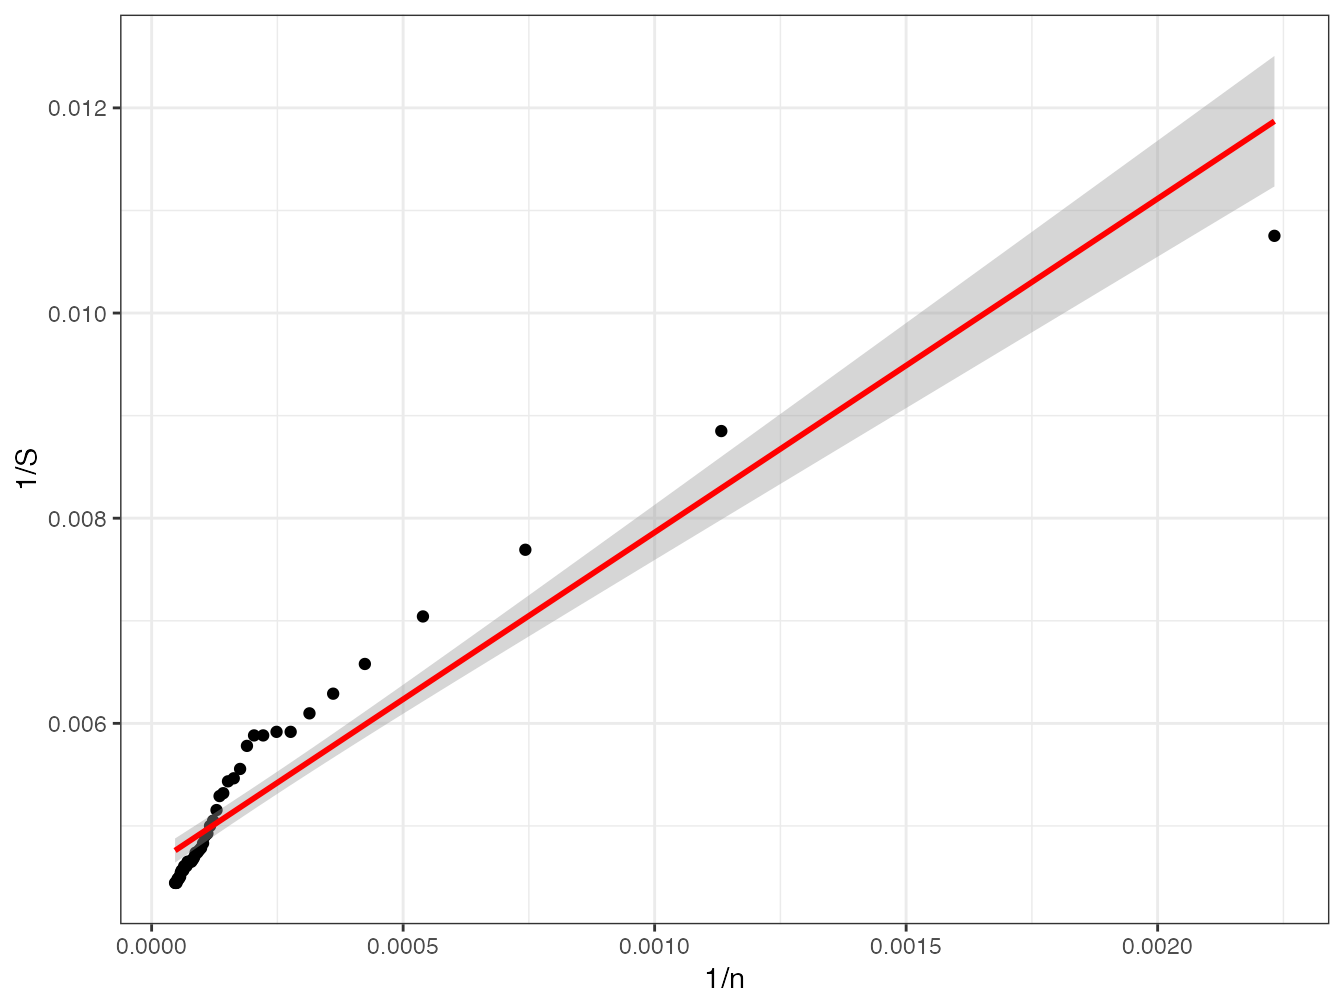
\includegraphics[width=0.8\linewidth]{MesuresBD_files/figure-latex/LineweaverFig-1} 

}

\caption{Ajustement du même modèle de Michaelis-Menten transformé selon Lineweaver et Burk.}\label{fig:LineweaverFig}
\end{SCfigure}

\normalsize

On voit assez clairement que le modèle (figure \ref{fig:LineweaverFig}) s'ajuste mal quand il est représenté sous cette forme \autocite{Raaijmakers1987}.

Le code R nécessaire pour réaliser la figure est:

\scriptsize

\begin{Shaded}
\begin{Highlighting}[]
\KeywordTok{ggplot}\NormalTok{(}\KeywordTok{data.frame}\NormalTok{(x, y), }\KeywordTok{aes}\NormalTok{(x, y)) }\OperatorTok{+}\StringTok{ }
\StringTok{  }\KeywordTok{geom_point}\NormalTok{() }\OperatorTok{+}
\StringTok{  }\KeywordTok{stat_smooth}\NormalTok{(}\DataTypeTok{method =} \StringTok{"lm"}\NormalTok{, }\DataTypeTok{col =} \StringTok{"red"}\NormalTok{) }\OperatorTok{+}
\StringTok{  }\KeywordTok{labs}\NormalTok{(}\DataTypeTok{x =} \StringTok{"1/n"}\NormalTok{, }\DataTypeTok{y=}\StringTok{"1/S"}\NormalTok{)}
\end{Highlighting}
\end{Shaded}

\normalsize

Le nombre d'espèces estimé est inférieur au nombre observé, qui ne se trouve même pas dans l'intervalle de confiance à 95\%.
Le modèle de Michaelis-Menten ne convient pas.

\textcite{Soberon1993} développent un cadre théorique plus vaste qui permet d'ajuster la courbe d'accumulation à plusieurs modèles.
Ces modèles sont efficaces empiriquement mais manquent de support théorique pour justifier leur forme.
Le modèle le plus simple est exponentiel négatif.
Si la probabilité de trouver une nouvelle espèce est proportionnelle au nombre d'espèces non encore découvertes, la courbe d'accumulation suit la relation

\begin{equation} 
  \label{eq:Soberon1993a}
  S^{n} = S \left( 1 - e^{Kn} \right).
\end{equation}

Les paramètres peuvent être estimés par la méthode des moindres carrés:

\scriptsize

\begin{Shaded}
\begin{Highlighting}[]
\NormalTok{(nlsexp <-}\StringTok{ }\KeywordTok{nls}\NormalTok{(nEspeces }\OperatorTok{~}\StringTok{ }\NormalTok{S }\OperatorTok{*}\StringTok{ }\NormalTok{(}\DecValTok{1} \OperatorTok{-}\StringTok{ }\KeywordTok{exp}\NormalTok{(K }\OperatorTok{*}\StringTok{ }\NormalTok{nArbres)), }\DataTypeTok{data =} \KeywordTok{list}\NormalTok{(nArbres, }
\NormalTok{    nEspeces), }\DataTypeTok{start =} \KeywordTok{list}\NormalTok{(}\DataTypeTok{S =} \KeywordTok{max}\NormalTok{(nEspeces), }\DataTypeTok{K =} \DecValTok{-1}\OperatorTok{/}\DecValTok{1000}\NormalTok{)))}
\end{Highlighting}
\end{Shaded}

\begin{verbatim}
## Nonlinear regression model
##   model: nEspeces ~ S * (1 - exp(K * nArbres))
##    data: list(nArbres, nEspeces)
##          S          K 
## 212.198082  -0.000494 
##  residual sum-of-squares: 10664
## 
## Number of iterations to convergence: 13 
## Achieved convergence tolerance: 8.042e-06
\end{verbatim}

\normalsize

Ce modèle, proposé par \textcite{Holdridge1971}, sous-estime la richesse parce que la probabilité de découvrir une nouvelle espèce diminue plus vite que le nombre d'espèces restant à découvrir: les dernières espèces sont plus rares et donc plus difficiles à détecter.

Un modèle plus réaliste définit cette probabilité comme une fonction décroissante du nombre d'espèces manquantes.
La fonction la plus simple est une exponentielle négative mais elle ne s'annule jamais et le nombre d'espèces n'a pas d'asymptote.
Un paramètre supplémentaire pour obtenir l'asymptote est nécessaire et aboutir à la relation

\begin{equation} 
  \label{eq:Soberon1993b}
  S^{n} = \frac{1}{z} \ln \left[ \frac{a}{c} - \frac{a-c}{c} e^{-czn} \right].
\end{equation}

Les paramètres à estimer sont \(z\), \(a\) et \(c\).

\scriptsize

\begin{Shaded}
\begin{Highlighting}[]
\NormalTok{(nlslog <-}\StringTok{ }\KeywordTok{nls}\NormalTok{(nEspeces }\OperatorTok{~}\StringTok{ }\DecValTok{1}\OperatorTok{/}\NormalTok{z }\OperatorTok{*}\StringTok{ }\KeywordTok{log}\NormalTok{(a}\OperatorTok{/}\NormalTok{c }\OperatorTok{-}\StringTok{ }\NormalTok{(a }\OperatorTok{-}\StringTok{ }\NormalTok{c)}\OperatorTok{/}\NormalTok{c }\OperatorTok{*}\StringTok{ }\KeywordTok{exp}\NormalTok{(}\OperatorTok{-}\NormalTok{c }\OperatorTok{*}\StringTok{ }
\StringTok{    }\NormalTok{z }\OperatorTok{*}\StringTok{ }\NormalTok{nArbres)), }\DataTypeTok{data =} \KeywordTok{list}\NormalTok{(nArbres, nEspeces), }\DataTypeTok{start =} \KeywordTok{list}\NormalTok{(}\DataTypeTok{z =} \FloatTok{0.05}\NormalTok{, }
    \DataTypeTok{a =} \DecValTok{1}\NormalTok{, }\DataTypeTok{c =} \FloatTok{0.001}\NormalTok{)))}
\end{Highlighting}
\end{Shaded}

\begin{verbatim}
## Nonlinear regression model
##   model: nEspeces ~ 1/z * log(a/c - (a - c)/c * exp(-c * z * nArbres))
##    data: list(nArbres, nEspeces)
##        z        a        c 
## 0.025139 0.755365 0.001114 
##  residual sum-of-squares: 446.1
## 
## Number of iterations to convergence: 4 
## Achieved convergence tolerance: 4.813e-06
\end{verbatim}

\begin{Shaded}
\begin{Highlighting}[]
\CommentTok{# Nombre d'espèces}
\NormalTok{coefs <-}\StringTok{ }\KeywordTok{coef}\NormalTok{(nlslog)}
\KeywordTok{log}\NormalTok{(coefs[}\StringTok{"a"}\NormalTok{]}\OperatorTok{/}\NormalTok{coefs[}\StringTok{"c"}\NormalTok{])}\OperatorTok{/}\NormalTok{coefs[}\StringTok{"z"}\NormalTok{]}
\end{Highlighting}
\end{Shaded}

\begin{verbatim}
##        a 
## 259.3128
\end{verbatim}

\normalsize



\scriptsize

\begin{SCfigure}

{\centering 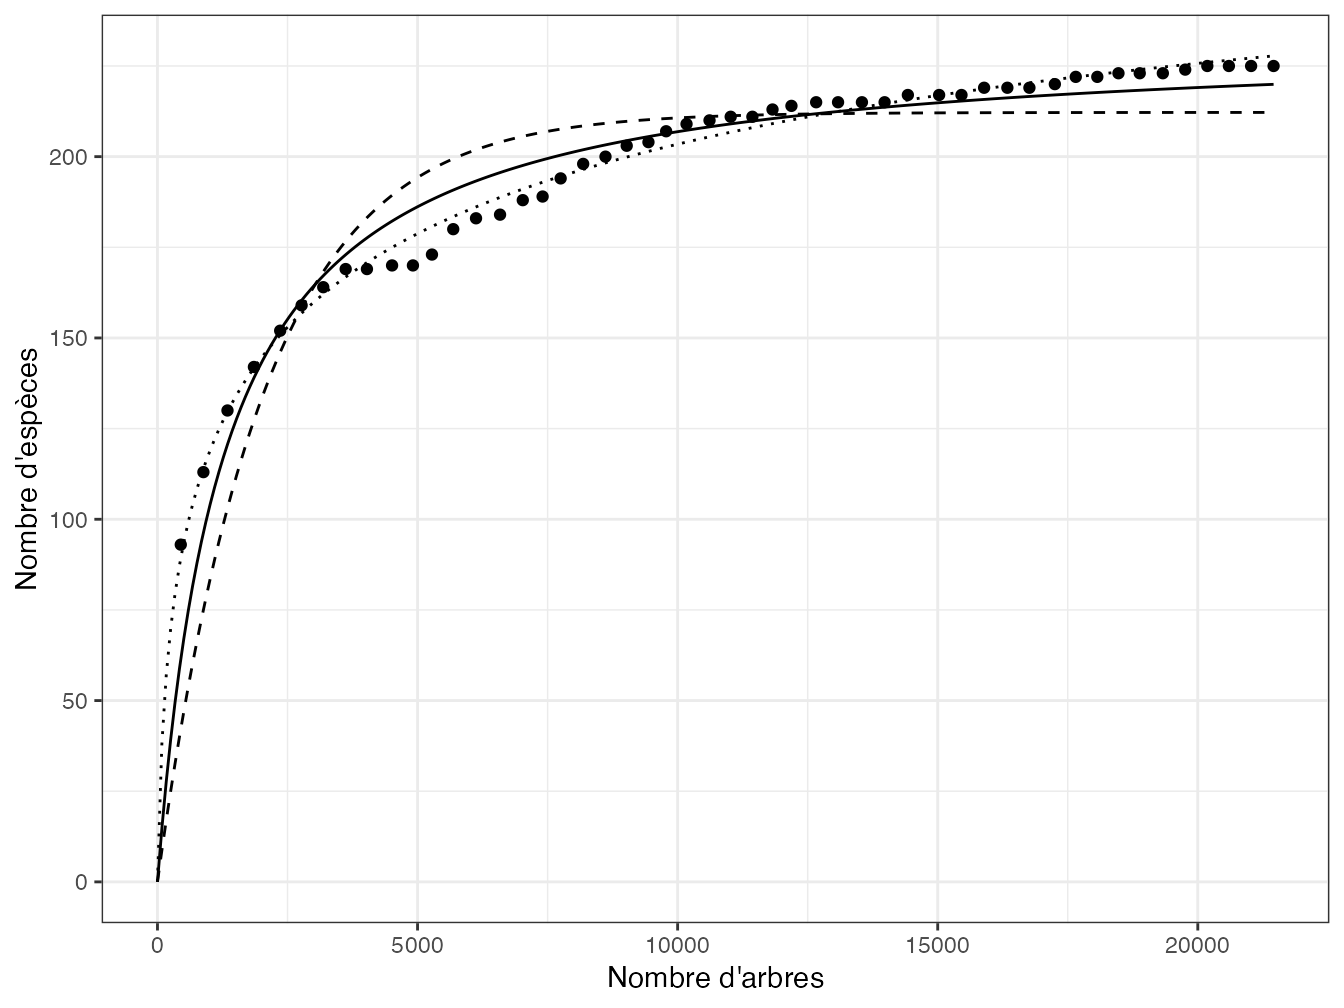
\includegraphics[width=0.8\linewidth]{MesuresBD_files/figure-latex/SobLLorFig-1} 

}

\caption{Ajustement des modèle de Michaelis-Menten (trait plein) et de de Soberón et Llorente (pointillés longs: modèle exponentiel négatif; pointillés courts: modèle à trois paramètres) aux données de BCI. Les cercles représentent le nombre d'espèces cumulées en fonction du nombre d'arbres. Le modèle exponentiel négatif (Holdridge) sous-estime la richesse, plus que celui de Michaelis-Menten (Clench). Le modèle à trois paramètres s'ajuste mieux aux données, mais il surestime probablement la richesse.}\label{fig:SobLLorFig}
\end{SCfigure}

\normalsize

L'estimation est cette fois supérieure à celle du jackknife (244 espèces).

La figure \ref{fig:SobLLorFig} présente les deux ajustements de modèle de Soberón et Llorente avec celui de Clench.
L'estimation de la richesse par extrapolation est plus incertaine que par les méthodes non paramétriques.
Elle est très peu utilisée.

Le code R nécessaire pour réaliser la figure est:

\scriptsize

\begin{Shaded}
\begin{Highlighting}[]
\NormalTok{x <-}\StringTok{ }\KeywordTok{seq}\NormalTok{(}\DataTypeTok{from =} \DecValTok{0}\NormalTok{, }\DataTypeTok{to =} \KeywordTok{max}\NormalTok{(nArbres), }\DataTypeTok{length =} \DecValTok{255}\NormalTok{)}
\NormalTok{NewData <-}\StringTok{ }\KeywordTok{list}\NormalTok{(}\DataTypeTok{nArbres =}\NormalTok{ x)}
\KeywordTok{ggplot}\NormalTok{(}\KeywordTok{data.frame}\NormalTok{(x, }
        \DataTypeTok{MM =} \KeywordTok{predict}\NormalTok{(nlsfit, }\DataTypeTok{newdata =}\NormalTok{ NewData),}
        \DataTypeTok{Holdridge =} \KeywordTok{predict}\NormalTok{(nlsexp, }\DataTypeTok{newdata =}\NormalTok{ NewData),}
        \DataTypeTok{Soberon =} \KeywordTok{predict}\NormalTok{(nlslog, }\DataTypeTok{newdata =}\NormalTok{ NewData)), }
    \KeywordTok{aes}\NormalTok{(x)) }\OperatorTok{+}
\StringTok{  }\KeywordTok{geom_point}\NormalTok{(}\KeywordTok{aes}\NormalTok{(nArbres, nEspeces), }\KeywordTok{data.frame}\NormalTok{(nArbres, nEspeces)) }\OperatorTok{+}
\StringTok{  }\KeywordTok{geom_line}\NormalTok{(}\KeywordTok{aes}\NormalTok{(}\DataTypeTok{y =}\NormalTok{ MM)) }\OperatorTok{+}
\StringTok{  }\KeywordTok{geom_line}\NormalTok{(}\KeywordTok{aes}\NormalTok{(}\DataTypeTok{y =}\NormalTok{ Holdridge), }\DataTypeTok{lty =} \DecValTok{2}\NormalTok{) }\OperatorTok{+}
\StringTok{  }\KeywordTok{geom_line}\NormalTok{(}\KeywordTok{aes}\NormalTok{(}\DataTypeTok{y =}\NormalTok{ Soberon), }\DataTypeTok{lty =} \DecValTok{3}\NormalTok{) }\OperatorTok{+}
\StringTok{  }\KeywordTok{labs}\NormalTok{(}\DataTypeTok{x =} \StringTok{"Nombre d'arbres"}\NormalTok{, }\DataTypeTok{y =} \StringTok{"Nombre d'espèces"}\NormalTok{)}
\end{Highlighting}
\end{Shaded}

\normalsize

\hypertarget{diversituxe9-guxe9nuxe9rique}{%
\subsection{Diversité générique}\label{diversituxe9-guxe9nuxe9rique}}

La détermination des genres est plus facile et fiable que celle des espèces, le biais d'échantillonnage moins sensible (le nombre de singletons diminue rapidement en regroupant les données), et les coûts d'inventaire sont généralement largement réduits \autocite{Balmford1996b}.
Le choix d'estimer la diversité de taxons de rang supérieur (genres ou même familles au lieu des espèces) est envisageable \autocite{Williams1994}.

Empiriquement, la corrélation entre la richesse générique et la richesse spécifique (des angiospermes, des oiseaux et des mammifères) est bonne en forêt tropicale \autocite{Balmford1996a}, suffisante pour comparer les communautés, même si la prédiction de la richesse spécifique à partir de la richesse générique est très imprécise.

\textcite{Cartozo2008} ont montré que le nombre de taxons de niveau supérieur (genre par rapport aux espèces, ordres par rapport aux sous-ordres) est universellement proportionnel au nombre de taxons du niveau immédiatement inférieur à la puissance 0,61. Cette relation est validée à l'échelle mondiale pour les systèmes végétaux. La loi de puissance reste valide pour des assemblages aléatoires, c'est donc la conséquence de propriétés mathématiques \autocite{Caldarelli2002}, mais la puissance de la relation est plus élevée (les communautés réelles sont plus agrégées du point de vue phylogénétique que sous l'hypothèse nulle d'un assemblage aléatoire) et varie entre les niveaux.

\hypertarget{combien-y-a-t-il-despuxe8ces-diffuxe9rentes-sur-terre}{%
\subsection{Combien y a-t-il d'espèces différentes sur Terre?}\label{combien-y-a-t-il-despuxe8ces-diffuxe9rentes-sur-terre}}

La question de l'estimation du nombre total d'espèces génère une abondante littérature.
\textcite{Mora2011} en font une revue et proposent une méthode nouvelle.

Dans chaque règne, le nombre de taxons de niveaux supérieurs (phylums, classes, ordres, familles et même genres) est estimé par des modèles prolongeant jusqu'à leur asymptote les valeurs connues en fonction du temps.
Cette méthode est applicable jusqu'au niveau du genre (figure \ref{fig:Mora2011}, A à E).
Le nombre de taxon de chaque niveau est lié à celui du niveau précédent, ce qui est représenté par la figure \ref{fig:Mora2011}, G \autocite[figure 1]{Mora2011} sous la forme du relation linéaire entre le logarithme du logarithme du nombre de taxons et le rang (1 pour les phylums, 5 pour les genres).
La droite est prolongée jusqu'au rang 6 pour obtenir le nombre d'espèces.
Une façon alternative de décrire la méthode est de dire que le nombre de taxons du niveau \(n+1\) est égal à celui du niveau \(n\) à la puissance \(k\).
La pente de la droite de la figure est \(\ln{k}\).
Aucune justification de ce résultat majeur n'est donnée par les auteurs, si ce n'est leur vérification empirique.

Le nombre total d'espèces estimé est 8,7 millions, tous règnes confondus, dans la fourchette des estimations précédentes (de 3 à 100 millions), et nécessitant près de 500 ans d'inventaires au rythme actuel des découvertes \autocite{May2011}.



\scriptsize

\begin{SCfigure}

{\centering 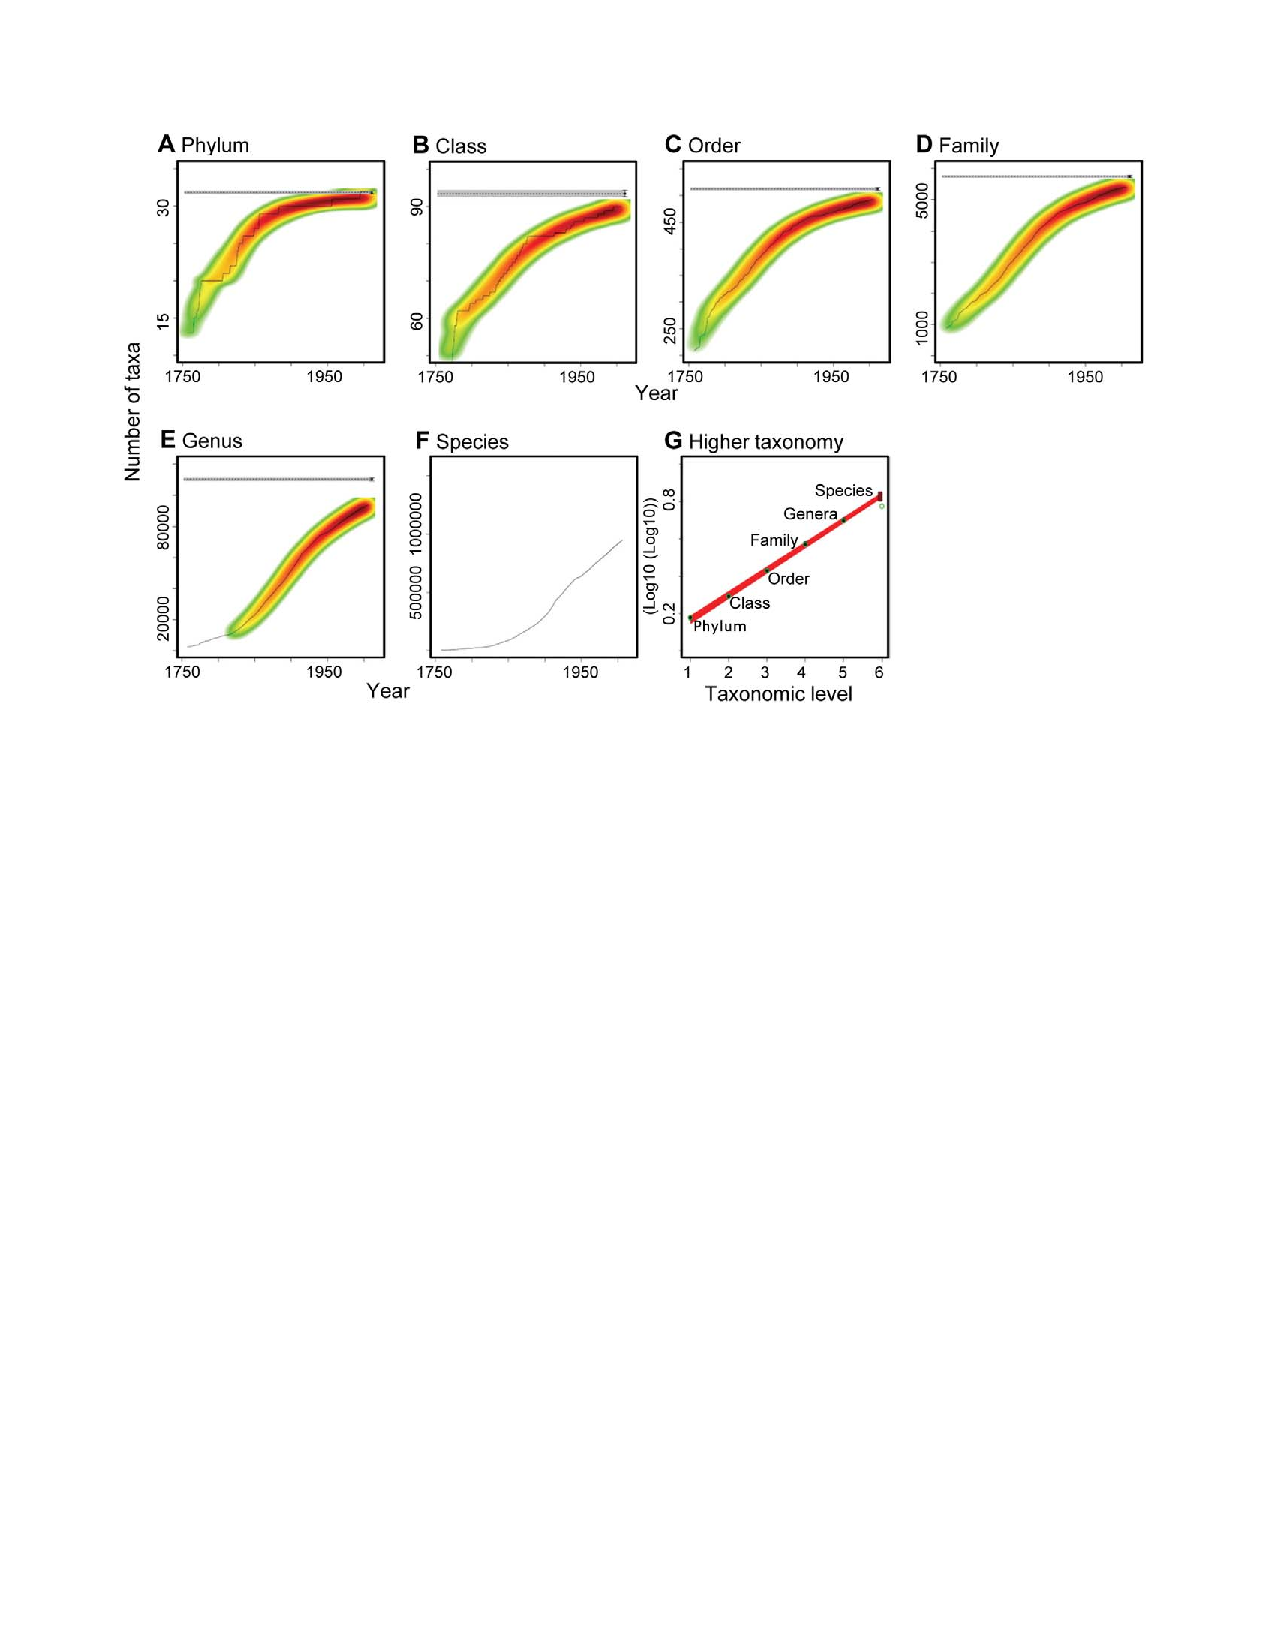
\includegraphics[width=0.8\linewidth]{images/Mora2011} 

}

\caption{Évolution du nombre de taxons connus en fonction du temps et valeur estimée du nombre total (ligne horizontale grise, A à E). Le nombre d'espèces connues est trop faible pour utiliser cette méthode (F). Il est obtenu par extrapolation de la relation du nombre de taxons d'un niveau à celui du niveau supérieur (G).}\label{fig:Mora2011}
\end{SCfigure}

\normalsize

En se limitant aux arbres, l'estimation se monte à 16000 espèces pour l'Amazonie \autocite{TerSteege2013}, de l'ordre de 5000 pour l'Afrique et entre 40000 et 53000 pour l'ensemble des tropiques \autocite{Slik2015} (donc pour l'ensemble de la planète, le nombre d'espèces non-tropicales étant négligeable).
Ces estimations sont obtenues par extrapolation du modèle en log-séries (chapitre \ref{chap:Fisher}) et sont sujettes au paradoxe de Fisher: les espèces représentées par un très petit nombre d'individu dans le modèle, notamment les singletons, sont les plus nombreuses.
Une discussion approfondie est donnée par \textcite{Hubbell2015}: les espèces récemment apparues au sens du modèle ne sont pas détectables avant plusieurs générations, créant un décalage entre le nombre d'espèces reconnues par la taxonomie et modèle.

\textcite{Wilson2012} compilent les relevés du nombre d'espèces de plantes vasculaires en fonction de la surface et retiennent uniquement les plus riches à chaque échelle spatiale (du millimètre carré à l'hectare).
Ces relevés sont tous situés en forêt tropicale ou en prairie tempérée gérée (les perturbations régulières et modérées y favorisent la diversité, conformément à la théorie de la perturbation intermédiaire \autocite{Connell1978}).
La relation entre le nombre d'espèces et la surface est celle d'Arrhenius.
Son extrapolation à la surface terrestre donne environ 220000 espèces, comparables à l'estimation de 275000 espèces rapportée par Mora et al.

\hypertarget{indice-de-simpson}{%
\section{Indice de Simpson}\label{indice-de-simpson}}

\hypertarget{duxe9finition}{%
\subsection{Définition}\label{duxe9finition}}

On note \(p_s\) la probabilité qu'un individu tiré au hasard appartienne à l'espèce \(s\).
L'indice de \textcite{Simpson1949}, ou Gini-Simpson, est

\begin{equation}
  \label{eq:SimpsonE}
  E =1-\sum^{S}_{s=1}{p^2_s}.
\end{equation}

Il peut être interprété comme la probabilité que deux individus tirés au hasard soient d'espèces différentes.
Il est compris dans l'intervalle \(\left[0;1\right[\).
Sa valeur diminue avec la régularité de la distribution: \(E=0\) si une seule espèce a une probabilité de 1, \(E=1-{1}/{S}\) si les \(S\) espèces ont la même probabilité \(p_s={1}/{S}\).
La valeur 1 est atteinte pour un nombre infini d'espèces, de probabilités nulles.

Deux autres formes de l'indice sont utilisées.
Tout d'abord, la probabilité que deux individus soient de la même espèce, souvent appelée \emph{indice de concentration de Simpson}, qui est celui défini dans l'article original de Simpson:

\begin{equation}
  \label{eq:SimpsonD}
  D =\sum^{S}_{s=1}{p^2_s}.
\end{equation}

L'indice de Simpson est parfois considéré comme une mesure d'équitabilité \autocite{Olszewski2004} mais il varie avec la richesse: cette approche est donc erronnée.
\textcite{Hurlbert1971} l'a divisé par sa valeur maximale \(1-{1}/{S}\) pour obtenir une mesure d'équitabilité valide généralisée plus tard par \textcite{Mendes2008}, voir section \ref{sec:Mendes}.
Le nombre d'espèces doit être estimé par les méthodes présentées plus haut, pour ne pas dépendre de la taille de l'échantillon.

L'estimateur du maximum de vraisemblance de l'indice est

\begin{equation}
  \label{eq:EstEML}
  \hat{E} = 1-\sum^{s^{n}_{\ne 0}}_{s=1}{\hat{p}^2_s}.
\end{equation}

Le calcul de l'indice de Simpson peut se faire avec la fonction \texttt{diversity} disponible dans le package \emph{vegan} de R ou avec la fonction \texttt{Simpson} du package \emph{entropart}:

\scriptsize

\begin{Shaded}
\begin{Highlighting}[]
\KeywordTok{data}\NormalTok{(BCI)}
\CommentTok{# as.ProbaVector() transforme les abondances en probabilités}
\NormalTok{Ps <-}\StringTok{ }\KeywordTok{as.ProbaVector}\NormalTok{(}\KeywordTok{colSums}\NormalTok{(BCI))}
\KeywordTok{Simpson}\NormalTok{(Ps)}
\end{Highlighting}
\end{Shaded}

\begin{verbatim}
##      None 
## 0.9736755
\end{verbatim}

\normalsize

Un historique de la définition de l'indice, de \textcite{Gini1912} à Simpson, inspiré par Turing, est fourni par Ellerman \autocite*{Ellerman2013}.

\hypertarget{estimation}{%
\subsection{Estimation}\label{estimation}}

Définissons l'indicatrice \({{\mathbf 1}}_{sh}\) valant 1 si l'individu \(h\) appartient à l'espèce \(s\), 0 sinon.
\({{\mathbf 1}}_{sh}\) suit une loi de Bernoulli d'espérance \(p_s\) et de variance \(p_s\left(1-p_s\right)\).
\(E\) est la somme sur toutes les espèces de cette variance.
Un estimateur non biaisé d'une variance à partir d'un échantillon est la somme des écarts quadratiques divisée par le nombre d'observation moins une.
L'estimateur \(\hat{E}\) est légèrement biaisé parce qu'il est calculé à partir des \({\hat{p}}_s\), ce qui revient à diviser la somme des écarts par \(n\), et non \(n-1\).
Un estimateur non biaisé est \autocite{Good1953,Lande1996}

\begin{equation} 
  \label{eq:BiaisSimpson}
  \tilde{E} = \left(\frac{n}{n-1}\right)\left(1-\sum^{s^{n}_{\ne 0}}_{s=1}{{\hat{p}}^2_s}\right).
\end{equation}

La correction par \({n}/{\left(n-1\right)}\) tend rapidement vers 1 quand la taille de l'échantillon augmente: l'estimateur est très peu biaisé.

Le non-échantillonnage des espèces rares est pris en compte dans cette correction parce qu'elle considère que \(\tilde{E}\) est l'estimateur de variance d'un échantillon et non d'une population complètement connue.
Il est négligeable: si \(p_s\) est petit, \(p^2_s\) est négligeable dans la somme.

Simpson a fourni un estimateur non biaisé de \(D\), à partir du calcul du nombre de paires d'individus tirés sans remise:

\begin{equation}
  \label{eq:EstSimpson1949}
  \tilde{D} = \frac{\sum^{S}_{s=1}{n_s\left(n_s -1\right)}}{n\left(n-1\right)}.
\end{equation}

L'argumentation est totalement différente, mais le résultat est le même: \(\tilde{E}=1-\tilde{D}\).

La fonction \texttt{Simpson} de \emph{entropart} accepte comme argument un vecteur d'abondances et propose par défaut la correction de Lande:

\scriptsize

\begin{Shaded}
\begin{Highlighting}[]
\KeywordTok{Simpson}\NormalTok{(}\KeywordTok{colSums}\NormalTok{(BCI))}
\end{Highlighting}
\end{Shaded}

\begin{verbatim}
##     Lande 
## 0.9737209
\end{verbatim}

\normalsize

\hypertarget{indice-de-shannon}{%
\section{Indice de Shannon}\label{indice-de-shannon}}

\hypertarget{duxe9finition-1}{%
\subsection{Définition}\label{duxe9finition-1}}

L'indice de Shannon \autocite{Shannon1948,Shannon1963}, aussi appelé indice de Shannon-Weaver ou Shannon-Wiener \autocite{Spellerberg2003}, ou simplement \emph{entropie} est dérivé de la théorie de l'information:

\begin{equation}
  \label{eq:Shannon}
  H = -\sum^S_{s=1}{p_s\ln{p_s}}.
\end{equation}

Considérons une placette forestière contenant \(S\) espèces végétales différentes.
La probabilité qu'une plante choisie au hasard appartienne à l'espèce \(s\) est notée \(p_s\).
On prélève \(n\) plantes, et on enregistre la liste ordonnée des espèces des \(n\) plantes.
Si \(n\) est suffisamment grand, le nombre de plantes de l'espèce \(s\) est \(np_s\).
On note \(L\) le nombre de listes respectant ces conditions:

\begin{equation}
  \label{eq:ShannonL}
  L = \frac{n!}{\prod^S_{i=1}{\left({np}_s\right)!}}.
\end{equation}

Ce résultat est obtenu en calculant le nombre de positions possibles dans la liste pour les individus de la première espèce: \(\binom{n}{np_1}\).
Le nombre de positions pour la deuxième espèce est \(\binom{n-np_1}{np_2}\).
Pour la \(S\)-ième espèce, le nombre est \(\binom{n-np_1-\dots -np_{s-1}}{np_i}\).
Les produits de combinaisons se simplifient pour donner l'équation \eqref{eq:ShannonL}.

On peut maintenant écrire le logarithme de \(L\):
\[\ln{L}=\ln{n!}-\sum^S_{s=1}{\ln{np_s}!}.\]
On utilise l'approximation de Stirling,
\[\ln{n!}\approx n\ln{n}-n,\]
pour obtenir après simplifications:

\begin{equation}
  \label{eq:ShannonlnL}
  \ln{L} = -n\sum^S_{s=1}{p_s \ln{p_s}}.
\end{equation}

\(H=(\ln{L})/{n}\) est l'indice de Shannon.
Ce résultat est connu sous le nom de formule de \textcite{Brillouin1962}.
À l'origine, Shannon a utilisé un logarithme de base 2 pour que \(H\) soit le nombre moyen de questions binaires (réponse oui ou non) nécessaire pour identifier l'espèce d'une plante (un caractère utilisé dans une chaîne dans le contexte du travail de Shannon).
Les logarithmes naturels, de base 2 ou 10 ont été utilisés par la suite \autocite{Pielou1966a}.

La formule \eqref{eq:ShannonlnL} est celle de l'indice de \textcite{Theil1967}, présenté en détail par \textcite{Conceicao2000}, à l'origine utilisé pour mesurer les inégalités de revenu puis pour caractériser les structures spatiales en économie.
L'indice est proportionnel au nombre de plantes choisies, on peut donc le diviser par \(n\) et on obtient l'indice de biodiversité de Shannon.
Ces indices ont été définis en choisissant des lettres au hasard pour former des chaînes de caractères.
Leur valeur est le nombre de chaînes de caractères différentes que l'on peut obtenir avec l'ensemble des lettres disponibles, c'est-à-dire la quantité d'information contenue dans l'ensemble des lettres.
L'indice de Shannon donne une mesure de la biodiversité en tant que quantité d'information.

L'estimateur du maximum de vraisemblance de l'indice est

\begin{equation}
  \label{eq:EstShannonML}
  \hat{H} = -\sum^{s^{n}_{\ne 0}}_{s=1}{\hat{p}_s \ln{\hat{p}_s}}.
\end{equation}

Le calcul de l'indice de Shannon peut se faire avec la fonction \texttt{diversity} disponible dans le package \emph{vegan} de R ou avec la fonction \texttt{Shannon} de \emph{entropart}:

\scriptsize

\begin{Shaded}
\begin{Highlighting}[]
\NormalTok{Ps <-}\StringTok{ }\KeywordTok{as.ProbaVector}\NormalTok{(}\KeywordTok{colSums}\NormalTok{(BCI))}
\KeywordTok{Shannon}\NormalTok{(Ps)}
\end{Highlighting}
\end{Shaded}

\begin{verbatim}
##     None 
## 4.270409
\end{verbatim}

\normalsize

La distribution de l'estimateur est connue \autocite{Hutcheson1970} mais elle est inutile en pratique à cause du biais d'estimation.

\textcite{Bulmer1974} établit une relation entre l'indice de Shannon et l'indice \(\alpha\) de Fisher, à condition que la distribution de l'abondance des espèces soit log-normale:

\begin{equation}
  \label{eq:Bulmer1974}
  \hat{H} = \mathrm{\Psi}\left(\hat{\alpha}+1\right) - \mathrm{\Psi}\left(1\right).
\end{equation}

\(\mathrm{\Psi}(\cdot)\) est la fonction digamma, et \(\hat{\alpha}\) est l'estimateur de l'indice de Fisher \eqref{eq:AlphaFisher}:

\scriptsize

\begin{Shaded}
\begin{Highlighting}[]
\KeywordTok{digamma}\NormalTok{(}\KeywordTok{fisher.alpha}\NormalTok{(}\KeywordTok{colSums}\NormalTok{(BCI)) }\OperatorTok{+}\StringTok{ }\DecValTok{1}\NormalTok{) }\OperatorTok{-}\StringTok{ }\KeywordTok{digamma}\NormalTok{(}\DecValTok{1}\NormalTok{)}
\end{Highlighting}
\end{Shaded}

\begin{verbatim}
## [1] 4.148322
\end{verbatim}

\normalsize

La sous-estimation est assez sévère sur cet exemple.

\hypertarget{sec:BiaisShannon}{%
\subsection{Estimation}\label{sec:BiaisShannon}}

\textcite{Basharin1959} a montré que l'estimateur de l'indice de Shannon était biaisé parce que des espèces ne sont pas échantillonnées.
Si \(S\) est le nombre d'espèces réel et \(n\) le nombre d'individus échantillonnés, le biais est

\begin{equation}
  \label{eq:Basharin1959}
  \mathbb{E}\left(\hat{H}\right)-H =-\frac{S-1}{2n} + O\left(n^{-2}\right).
\end{equation}

\(O\left(n^{-2}\right)\) est un terme négligeable.
La valeur estimée à partir des données est donc trop faible, d'autant plus que le nombre d'espèces total est grand mais d'autant moins que l'échantillonnage est important.
Comme le nombre d'espèces \(S\) n'est pas observable, le biais réel est inconnu.

L'estimateur de Miller-Madow \autocite{Miller1955} utilise l'information disponible, en sous-estimant le nombre d'espèces et donc l'entropie:
\begin{equation}
  \label{eq:MillerMadow}
  \tilde{H} = -\sum^{s^{n}_{\ne 0}}_{s=1}{\hat{p}_s \ln{\hat{p}_s}} + \frac{s^{n}_{\ne 0}-1}{2n}.
\end{equation}

\textcite{Chao2003} établissent un estimateur moins biaisé à partir du taux de couverture de l'échantillonnage \(\hat{C}\):

\begin{equation}
  \label{eq:ChaoShen}
  \tilde{H} = -\sum_{s=1}^{s^{n}_{\ne 0}}{\frac{\hat{C}{\hat{p}}_s \ln\left(\hat{C}{\hat{p}}_s\right)}{1-\left(1-\hat{C}{\hat{p}}_s\right)^n}}.
\end{equation}

Multiplier les fréquences observées par le taux de couverture permet d'obtenir un estimateur non biaisé des probabilités conditionnellement aux espèces non observées \autocite{Ashbridge2000}.

Le terme au dénominateur est la correction de \textcite{Horvitz1952}: chaque terme de la somme est divisé par la probabilité d'observer au moins une fois l'espèce correspondante.
Il tend vers 1 quand la taille de l'échantillon augmente.

\textcite{Beck2010} montrent que la correction du biais est efficace, même à des niveaux de complétude de l'échantillonnage (voir section \ref{sec:ChoixEstimateur}) très faibles. \textcite{Vu2007} étudient la vitesse de convergence de l'estimateur.

\textcite{Zhang2012} définit l'indice de Simpson généralisé:

\begin{equation}
  \label{eq:zeta}
  \zeta_{u,v} = \sum^S_{s=1}{p^u_s{\left(1-p_s\right)}^v},
\end{equation}

où \(\zeta_{u,v}\) est la somme sur toutes les espèces de la probabilité de rencontrer \(u\) fois l'espèce dans un échantillon de taille \(u+v\).
L'indice de Shannon peut s'exprimer en fonction de \(\zeta_{1,v}\):

\begin{equation}
  \label{eq:HzetaInf}
  H = \sum^{\infty}_{v=1}{\frac{1}{v} \zeta_{1,v}}.
\end{equation}

Les premiers termes de la somme, jusqu'à \(v=n-1\) peuvent être estimés à partir des données, les suivants constituent le biais de l'estimateur, qui est caculé en pratique par

\begin{equation}
  \label{eq:Hzetanu}
  H_z = \sum^{n-1}_{v=1}{\frac{1}{v}\left\{\frac{n^{v+1}\left[n-\left(v+1\right)\right]!}{n!}\sum^{s^{n}_{\ne 0}}_{s=1}{p_s\prod^{v-1}_{j=0}{\left(1-{\hat{p}}_s-\frac{j}{n}\right)}}\right\}}.
\end{equation}

\textcite{Zhang2013a} montre que le biais de l'estimateur \(H_z\) est asymptotiquement normal et calcule sa variance.
\textcite{Zhang2013} améliorent l'estimateur en le complétant par un estimateur de son biais, mais les calculs deviennent excessivement complexes.
\textcite{Vinck2012} appliquent la même démarche avec un estimateur bayesien du biais, utilisant un prior aussi plat que possible pour la valeur de l'entropie (et non un prior plat sur les probabilités, qui tire l'estimateur vers l'entropie maximale).
Cet estimateur nécessite de connaître le nombre d'espèces, ce qui empêche son utilisation sur des données d'écologie.

\textcite{Pielou1966} a développé une autre méthode de correction de biais lorsque de nombreux relevés de petite taille sont disponibles.
\(\ln{L}\) est calculé pour un relevé choisi aléatoirement puis les données du premier relevé sont ajoutées à celles d'un autre, puis un autre jusqu'à ce que \(H=(\ln{L})/{n}\) n'augmente plus: la diversité augmente dans un premier temps mais se stabilise quand l'effet des espèces ajoutées est compensé par celui de la diminution de l'équitabilité due aux espèces présentes dans tous les relevés.
À partir de ce seuil, l'augmentation de \(\ln{L}\) par individu ajouté est calculée pour chaque relevé supplémentaire.
Son espérance, estimée par sa moyenne calculée en ajoutant tous les relevés disponibles, est \(\tilde{H}\).

\textcite{Chao2013} utilisent l'estimateur de la pente de la courbe de raréfaction, calculé précédemment \autocite{Chao2012b} pour estimer la richesse spécifique, pour fournir un estimateur extrêmement performant:

\begin{align}
  \label{eq:Chao2013}
  \tilde{H}
  = &-\sum_{s=1}^{s^{n}_{\ne 0}}
    {\frac{n_s}{n}\left(\mathrm{\Psi}\left(n\right) - \mathrm{\Psi}\left(n_s\right)\right)} \\
  &-\frac{s_{1}}{n} {\left(1-A\right)}^{1-n} \left(-{\ln\left( A \right)}-\sum^{n-1}_{r=1}{\frac{1}{r}{\left( 1-A \right)}^r}\right),
\end{align}

où \(\mathrm{\Psi}\left(\cdot\right)\) est la fonction digamma et \(A\) vaut:

\begin{itemize}
\tightlist
\item
  \(2s_{2}/{\left[\left(n-1\right) s_{1} +2s_{2}\right]}\) en présence de singletons et doubletons;
\item
  \(2/{\left[\left(n-1\right)\left(s_{1} -1\right)+2\right]}\) en présence de singletons seulement;
\item
  \(1\) en absence de singletons et doubletons.
\end{itemize}

Enfin, la littérature de physique statistique s'est abondamment intéressée à cette question (\textcite{Bonachela2008} en font une revue).
Le problème traité est la non-linéarité de l'indice de Shannon par rapport aux probabilités qui entraine un biais d'estimation.
La fonction logarithme fournit un exemple simple: l'espérance de \(\ln(p_s)\) n'est pas le logarithme de l'espérance de \(p_s\) parce que la fonction \(\ln\) est concave.
Chaque estimateur \({\hat{p}}_s\) fluctue autour de \(p_s\) mais vaut \(p_s\) en moyenne.
À cause de la concavité, \(\ln({\hat{p}}_s)\) est en moyenne inférieur à \(\ln(p_s)\): cette relation est connue sous le nom d'inégalité de \textcite{Jensen1906}.
L'indice de Shannon est concave (figure \ref{fig:ShannonFig}) donc son estimateur \eqref{eq:Shannon} est biaisé négativement, même sans prendre en considération les espèces non observées.



\scriptsize

\begin{SCfigure}

{\centering 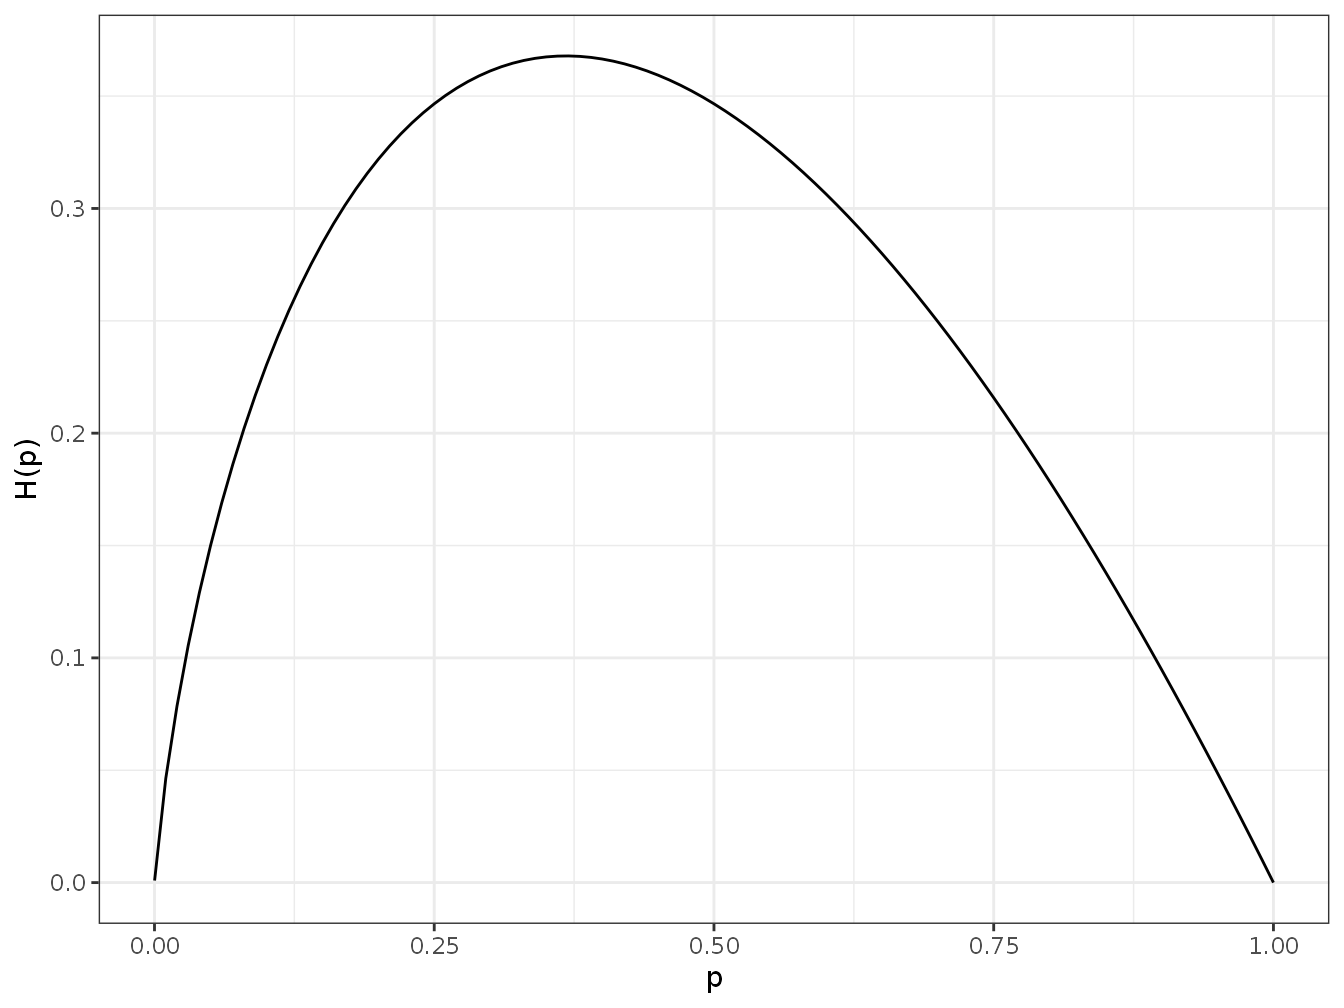
\includegraphics[width=0.8\linewidth]{MesuresBD_files/figure-latex/ShannonFig-1} 

}

\caption{Courbe de \(x\ln x\) entre 0 et 1.}\label{fig:ShannonFig}
\end{SCfigure}

\normalsize

Code de la figure \ref{fig:SARFig}:

\scriptsize

\begin{Shaded}
\begin{Highlighting}[]
\KeywordTok{ggplot}\NormalTok{(}\KeywordTok{data.frame}\NormalTok{(}\DataTypeTok{x =} \KeywordTok{c}\NormalTok{(}\FloatTok{0.0001}\NormalTok{, }\DecValTok{1}\NormalTok{)), }\KeywordTok{aes}\NormalTok{(x)) }\OperatorTok{+}\StringTok{ }
\StringTok{    }\KeywordTok{stat_function}\NormalTok{(}\DataTypeTok{fun =} \ControlFlowTok{function}\NormalTok{(x) }\OperatorTok{-}\NormalTok{x}\OperatorTok{*}\KeywordTok{log}\NormalTok{(x)) }\OperatorTok{+}
\StringTok{    }\KeywordTok{labs}\NormalTok{(}\DataTypeTok{x =} \StringTok{"p"}\NormalTok{, }\DataTypeTok{y =} \StringTok{"H(p)"}\NormalTok{)}
\end{Highlighting}
\end{Shaded}

\normalsize

Le biais peut être évalué par simulation: 10000 tirages sont réalisés dans une loi normale d'espérance \(p_s\) choisie et d'écart-type 0.01.
Le biais est la différence entre \({-p}_s{\ln p_s}\) (connu) et la moyenne des 1000 valeurs de \(-\hat{p}_s{\ln{\hat{p}}_s}\) (la probabilité est estimée par sa réalisation à chaque tirage).
La valeur du biais en fonction de \(p_s\) est en figure \ref{fig:ShannonBiaisFig}.
Le biais de l'indice de Shannon est la somme des biais pour toutes les probabilités spécifiques de la communauté étudiée, et son calcul est toujours l'objet de recherches.



\scriptsize

\begin{SCfigure}

{\centering 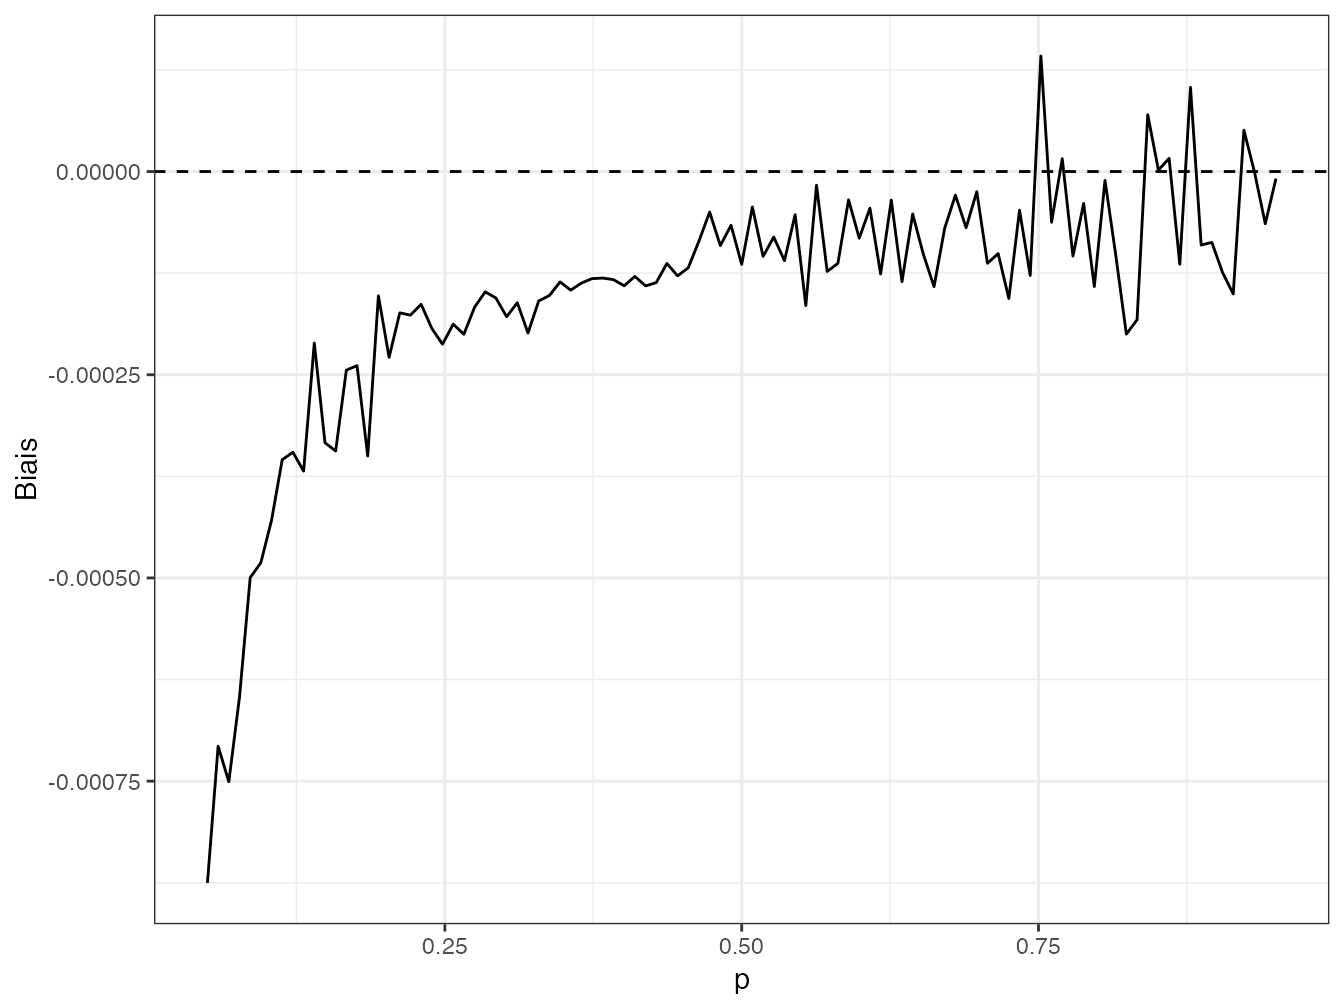
\includegraphics[width=0.8\linewidth]{MesuresBD_files/figure-latex/ShannonBiaisFig-1} 

}

\caption{Biais de \(\hat{p}_s \ln\hat{p}_s\) entre 0 et 1.}\label{fig:ShannonBiaisFig}
\end{SCfigure}

\normalsize

Code de la figure \ref{fig:ShannonBiaisFig}:

\scriptsize

\begin{Shaded}
\begin{Highlighting}[]
\NormalTok{Biais.p <-}\StringTok{ }\ControlFlowTok{function}\NormalTok{ (p) \{}
\NormalTok{    Ps <-}\KeywordTok{rnorm}\NormalTok{(}\DecValTok{10000}\NormalTok{, p, }\FloatTok{0.01}\NormalTok{)}
\NormalTok{    p }\OperatorTok{*}\StringTok{ }\KeywordTok{log}\NormalTok{(p) }\OperatorTok{-}\StringTok{ }\KeywordTok{mean}\NormalTok{(Ps }\OperatorTok{*}\StringTok{ }\KeywordTok{log}\NormalTok{(Ps))}
\NormalTok{  \}}
\NormalTok{  Biais <-}\StringTok{ }\ControlFlowTok{function}\NormalTok{ (Ps) \{}
    \CommentTok{# Applique Biais.p à chaque valeur de Ps}
    \KeywordTok{sapply}\NormalTok{(Ps, Biais.p)}
\NormalTok{  \}}
  \KeywordTok{ggplot}\NormalTok{(}\KeywordTok{data.frame}\NormalTok{(}\DataTypeTok{x =} \KeywordTok{c}\NormalTok{(}\FloatTok{0.05}\NormalTok{, }\FloatTok{0.95}\NormalTok{)), }\KeywordTok{aes}\NormalTok{(x)) }\OperatorTok{+}\StringTok{ }
\StringTok{    }\KeywordTok{stat_function}\NormalTok{(}\DataTypeTok{fun =}\NormalTok{ Biais) }\OperatorTok{+}
\StringTok{    }\KeywordTok{geom_hline}\NormalTok{(}\DataTypeTok{yintercept =} \DecValTok{0}\NormalTok{, }\DataTypeTok{lty =} \DecValTok{2}\NormalTok{) }\OperatorTok{+}
\StringTok{    }\KeywordTok{labs}\NormalTok{(}\DataTypeTok{x =} \StringTok{"p"}\NormalTok{, }\DataTypeTok{y =} \StringTok{"Biais"}\NormalTok{)}
\end{Highlighting}
\end{Shaded}

\normalsize

\textcite{Grassberger1988} a fourni la correction de référence:

\begin{equation}
  \label{eq:Grassberger1988}
  \tilde{H}
  = -\sum^{s^{n}_{\ne 0}}_{s=1}
  {\frac{n_s}{n}\left(\ln\left(n\right)-\mathrm{\Psi}\left(n_s\right)-\frac{{\left(-1\right)}^{n_s}}{n_s+1}\right)}.
\end{equation}

\textcite{Grassberger2003} l'a perfectionnée:

\begin{equation}
  \label{eq:Grassberger2003}
  \tilde{H} 
  = -\sum^{s^{n}_{\ne 0}}_{s=1}
    {\frac{n_s}{n} \left(\mathrm{\Psi}\left(n\right)-\mathrm{\Psi}\left(n_s\right)-{\left(-1\right)}^{n_s}\int^1_0{\frac{t^{n_s-1}}{1+t}\mathop{dt}}\right)}.
\end{equation}

Enfin, \textcite{Schurmann2004} l'a généralisée pour définir une famille de corrections dépendant d'un paramètre \(\xi\):

\begin{equation}
  \label{eq:Schurmann2004}
  \tilde{H} = -\sum^{s^{n}_{\ne 0}}_{s=1}
    {\frac{n_s}{n} \left(\mathrm{\Psi}\left(n\right)-\mathrm{\Psi}\left(n_s\right)-{\left(-1\right)}^{n_s}\int^{\frac{1}{\xi}-1}_0{\frac{t^{n_s-1}}{1+t}\mathop{dt}}\right)}.
\end{equation}

Le biais d'estimation diminue avec \(\xi\) mais l'erreur quadratique augmente.
Schürmann suggère d'utiliser \(\xi=e^{-{1}/{2}}\) comme meilleur compromis.

La fonction \texttt{Shannon} permet toutes ces corrections.
Elle accepte comme argument un vecteur d'abondances (et non de probabilités):

\scriptsize

\begin{Shaded}
\begin{Highlighting}[]
\KeywordTok{Shannon}\NormalTok{(}\KeywordTok{colSums}\NormalTok{(BCI), }\DataTypeTok{Correction =} \StringTok{"ChaoWangJost"}\NormalTok{)}
\end{Highlighting}
\end{Shaded}

\begin{verbatim}
## ChaoJost 
## 4.276193
\end{verbatim}

\begin{Shaded}
\begin{Highlighting}[]
\KeywordTok{Shannon}\NormalTok{(}\KeywordTok{colSums}\NormalTok{(BCI), }\DataTypeTok{Correction =} \StringTok{"Grassberger"}\NormalTok{)}
\end{Highlighting}
\end{Shaded}

\begin{verbatim}
## Grassberger 
##    4.276599
\end{verbatim}

\begin{Shaded}
\begin{Highlighting}[]
\KeywordTok{Shannon}\NormalTok{(}\KeywordTok{colSums}\NormalTok{(BCI), }\DataTypeTok{Correction =} \StringTok{"Grassberger2003"}\NormalTok{)}
\end{Highlighting}
\end{Shaded}

\begin{verbatim}
## Grassberger2003 
##        4.276491
\end{verbatim}

\begin{Shaded}
\begin{Highlighting}[]
\KeywordTok{Shannon}\NormalTok{(}\KeywordTok{colSums}\NormalTok{(BCI), }\DataTypeTok{Correction =} \StringTok{"Schurmann"}\NormalTok{)}
\end{Highlighting}
\end{Shaded}

\begin{verbatim}
## Schurmann 
##  4.276094
\end{verbatim}

\begin{Shaded}
\begin{Highlighting}[]
\KeywordTok{Shannon}\NormalTok{(}\KeywordTok{colSums}\NormalTok{(BCI), }\DataTypeTok{Correction =} \StringTok{"ZhangHz"}\NormalTok{)}
\end{Highlighting}
\end{Shaded}

\begin{verbatim}
##  ZhangHz 
## 4.272529
\end{verbatim}

\normalsize

D'autres estimateurs peu utilisés en écologie sont disponibles dans le package \emph{entropy} \autocite{Hausser2009}.
La contraction de Stein \autocite{James1961} consiste à estimer la distribution des probabilités d'occurence des espèces par la pondération optimale entre un estimateur à faible biais et un estimateur à faible variance.
L'estimateur \(\hat{p}_s\) est sans biais mais a une variance importante.
L'estimateur \({1}/{S}\), si \(S\) est connu, est de variance nulle mais est très biaisé.
Comme le nombre d'espèces est en général inconnu, il doit être estimé par une méthode quelconque, mais de préférence le surestimant plutôt que le sous-estimant.
L'estimateur de James-Stein (\emph{shrinkage estimator}) optimal est
\begin{equation}
  \label{eq:JamesStein1}
  \tilde{p}_s = \hat{\lambda}\frac{1}{\hat{S}} + \left( 1-\hat{\lambda} \right)\hat{p}_s,
\end{equation}

où
\begin{equation}
  \label{eq:JamesStein2}
  \hat{\lambda} = \frac{1-\sum^{s^{n}_{\ne 0}}_{s=1}{\left( \hat{p}_s \right)^2}}
                  {\left( n-1 \right) \sum^{s^{n}_{\ne 0}}_{s=1}{\left( \frac{1}{\hat{S}} - \hat{p}_s \right)^2}}.
\end{equation}

L'entropie est ensuite simplement estimée par l'estimateur plug-in: \(\tilde{H} = -\sum^{s^{n}_{\ne 0}}_{s=1}{\tilde{p}_s \ln{\tilde{p}_s}}\).
Le calcul sous R est le suivant:

\scriptsize

\begin{Shaded}
\begin{Highlighting}[]
\KeywordTok{library}\NormalTok{(}\StringTok{"entropy"}\NormalTok{)}
\KeywordTok{entropy.shrink}\NormalTok{(}\KeywordTok{colSums}\NormalTok{(BCI))}
\end{Highlighting}
\end{Shaded}

\begin{verbatim}
## Estimating optimal shrinkage intensity lambda.freq (frequencies): 0.0021
\end{verbatim}

\begin{verbatim}
## [1] 4.275689
## attr(,"lambda.freqs")
## [1] 0.002074043
\end{verbatim}

\normalsize

Le principe même de l'estimation rapproche la distribution de l'équiprobabilité des espèces et donc augmente l'entropie.
L'estimation précédente ignore les espèces non observées.
Pour les inclure, le vecteur des abondance doit être allongé par autant de zéros que d'espèces estimées:

\scriptsize

\begin{Shaded}
\begin{Highlighting}[]
\NormalTok{(S0 <-}\StringTok{ }\KeywordTok{jackknife}\NormalTok{(}\KeywordTok{AbdFreqCount}\NormalTok{(Ns))}\OperatorTok{$}\NormalTok{Nhat }\OperatorTok{-}\StringTok{ }\KeywordTok{ncol}\NormalTok{(BCI))}
\end{Highlighting}
\end{Shaded}

\begin{verbatim}
## 
## Your specified order is larger than that determined by the test, 
## Therefore the order from the test is used.
\end{verbatim}

\begin{verbatim}
## [1] 19
\end{verbatim}

\begin{Shaded}
\begin{Highlighting}[]
\KeywordTok{entropy.shrink}\NormalTok{(}\KeywordTok{c}\NormalTok{(}\KeywordTok{colSums}\NormalTok{(BCI), }\KeywordTok{rep}\NormalTok{(}\DecValTok{0}\NormalTok{, S0)))}
\end{Highlighting}
\end{Shaded}

\begin{verbatim}
## Estimating optimal shrinkage intensity lambda.freq (frequencies): 0.002
\end{verbatim}

\begin{verbatim}
## [1] 4.276543
## attr(,"lambda.freqs")
## [1] 0.002041748
\end{verbatim}

\normalsize

Les fréquences sont estimées par la fonction \texttt{freqs.shrink}.
Leur utilisation dans l'estimateur plug-in donne le même résultat:

\scriptsize

\begin{Shaded}
\begin{Highlighting}[]
\NormalTok{PsJS <-}\StringTok{ }\KeywordTok{freqs.shrink}\NormalTok{(}\KeywordTok{c}\NormalTok{(}\KeywordTok{colSums}\NormalTok{(BCI), }\KeywordTok{rep}\NormalTok{(}\DecValTok{0}\NormalTok{, S0)))}
\end{Highlighting}
\end{Shaded}

\begin{verbatim}
## Estimating optimal shrinkage intensity lambda.freq (frequencies): 0.002
\end{verbatim}

\begin{Shaded}
\begin{Highlighting}[]
\KeywordTok{Shannon}\NormalTok{(}\KeywordTok{as.ProbaVector}\NormalTok{(PsJS))}
\end{Highlighting}
\end{Shaded}

\begin{verbatim}
##     None 
## 4.276543
\end{verbatim}

\normalsize

Appliqué à des données de biodiversité aquatique, l'estimateur de James-Stein obtient de meilleurs résultats que celui de Chao et Shen \autocite{Liu2015} quand l'échantillonnage est réduit.

\hypertarget{sec:Hurlbert}{%
\section{Indice de Hurlbert}\label{sec:Hurlbert}}

\hypertarget{duxe9finition-2}{%
\subsection{Définition}\label{duxe9finition-2}}

L'indice de \textcite{Hurlbert1971} est l'espérance du nombre d'espèces observées dans un échantillon de taille \(k\) choisie:

\begin{equation}
  \label{eq:HurlbertSk}
  _{k}S = \sum^S_{s=1}{\left[1-{\left(1-p_s\right)}^k\right]}.
\end{equation}

Chaque terme de la somme est la probabilité d'observer au moins une fois l'espèce correspondante.

L'augmentation de la valeur de \(k\) permet de donner plus d'importance aux espèces rares.

L'indice peut être converti en nombre équivalent d'espèces \autocite{Dauby2012}, c'est-à-dire le nombre d'espèces équiprobables nécessaire pour obtenir la même diversité, notés \(_{k}D\) à partir de la relation

\begin{equation}
  \label{eq:HurlbertD}
  _{k}S = {_{k}D} \left[1-{\left(1-\frac{1}{_{k}D}\right)}^k\right].
\end{equation}

L'équation doit être résolue pour obtenir \(_{k}D\) à partir de la valeur de \(_{k}S\) estimée, numériquement pour \(k>3\).

Dans deux cas particuliers, les nombres équivalents d'espèces de Hurlbert sont identiques aux nombres de Hill: \(_{2}D ={^{2}\!D}\) et \(_{\infty}D={^{0}\!D}\).

Pour les autres ordres entiers de diversité, il existe une correspondance parfaite entre les deux mesures \autocite[Annexe S2]{Chao2014}: la connaissance de l'une permet d'obtenir l'autre. Pour \(k>1\), on a \autocite{Leinster2012}

\begin{equation}
  \label{eq:HurlbertDq}
  _{k}S = k + \sum_{q=2}^{k}{\binom{k}{q} (-1)^{q+1} (^{q}\!D)^{1-q}}.
\end{equation}

On a vu que \(^{0}\!D\) égale \(_{\infty}D\), donc \(_{\infty}S={^{0}\!D}\) \eqref{eq:HurlbertD}.

Inversement, pour \(q>1\):

\begin{equation}
  \label{eq:DqHurlbert}
  (^{q}\!D)^{1-q} = q + \sum_{k=2}^{q}{\binom{q}{k} (-1)^{k+1} _{k}S}.
\end{equation}

Pour \(q=1\), la relation est \autocite{Mao2007}
\begin{equation}
  \label{eq:Mao2007}
  ^{1}\!H = -1 + \sum_{k=2}^{\infty}{\frac{_{k}S}{k(k-1)}}.
\end{equation}

\hypertarget{estimation-1}{%
\subsection{Estimation}\label{estimation-1}}

Hurlbert fournit un estimateur non biaisé de son indice (\(n\) est la taille de l'échantillon, \(n_s\) le nombre d'individus de l'espèce \(s\)):

\begin{equation}
  \label{eq:EstHurlbert}
  _k{\tilde{S}}
  = \sum_{s=1}^{s^{n}_{\ne 0}}{\left[1-{\binom{n-n_s}{k}}/{\binom{n}{k}}\right]}.
\end{equation}

\textcite{Dauby2012} montrent que cet estimateur est très peu sensible à la taille de l'échantillon, et obtient de meilleurs résultats sur ce point que les estimateurs de Chao et Shen pour l'indice de Shannon ou du nombre d'espèces.
\textcite{Smith1977} ont calculé sa variance.

Le calcul de la diversité de Hurlbert est possible dans \emph{entropart}:

\scriptsize

\begin{Shaded}
\begin{Highlighting}[]
\CommentTok{# Indice de Hurlbert (probabilités)}
\KeywordTok{Hurlbert}\NormalTok{(}\KeywordTok{as.ProbaVector}\NormalTok{(}\KeywordTok{colSums}\NormalTok{(BCI)), }\DataTypeTok{k =} \DecValTok{2}\NormalTok{)}
\end{Highlighting}
\end{Shaded}

\begin{verbatim}
##   Biased 
## 1.973676
\end{verbatim}

\begin{Shaded}
\begin{Highlighting}[]
\CommentTok{# Estimateur sans biais (abondances)}
\KeywordTok{Hurlbert}\NormalTok{(}\KeywordTok{colSums}\NormalTok{(BCI), }\DataTypeTok{k =} \DecValTok{2}\NormalTok{)}
\end{Highlighting}
\end{Shaded}

\begin{verbatim}
## Unbiased 
## 1.973721
\end{verbatim}

\begin{Shaded}
\begin{Highlighting}[]
\CommentTok{# Nombre effectif d'espèces}
\KeywordTok{HurlbertD}\NormalTok{(}\KeywordTok{colSums}\NormalTok{(BCI), }\DataTypeTok{k =} \DecValTok{2}\NormalTok{)}
\end{Highlighting}
\end{Shaded}

\begin{verbatim}
## Unbiased 
## 38.05308
\end{verbatim}

\normalsize

\hypertarget{entropie}{%
\chapter{Entropie}\label{entropie}}

\scriptsize

\begin{Essentiel}
L'entropie est la surprise moyenne apportée par l'observation des
individus d'une communauté, d'autant plus grande qu'un individu
appartient à une espèce plus rare. L'entropie HCDT permet d'unifier les
indices classiques de diversité: son paramètre, appelé ordre, fixe
l'importance donnée aux espèces rares. L'entropie d'ordre 0 est la
richesse; celle d'ordre 1, l'indice de Shannon; celle d'ordre 2, celui
de Simpson. L'entropie est la moyenne du logarithme déformé de la rareté
des espèces, définie comme l'inverse de leur probabilité.

L'entropie va de pair avec la diversité au sens strict (Nombres de
Hill): le nombre d'espèces équiprobables dont l'entropie est la même que
celle de la communauté réelle. La diversité est l'exponentielle déformée
de l'entropie. Les profils de diversité représentent la diversité en
fonction de son ordre et permettent la comparaison de communautés.

L'estimation de la diversité est difficile pour des ordres inférieurs à
\(0,5\) dans des taxocènes très divers comme les arbres des forêts
tropicales.
\end{Essentiel}

\normalsize

L'entropie peut être entendue comme la surprise moyenne fournie par l'observation d'un échantillon.
C'est intuitivement une bonne mesure de diversité \autocite{Pielou1975}.
Ses propriétés mathématiques permettent d'unifier les mesures de diversité dans un cadre général.

\hypertarget{duxe9finition-de-lentropie}{%
\section{Définition de l'entropie}\label{duxe9finition-de-lentropie}}

Les textes fondateurs sont \textcite{Davis1941} et surtout \textcite{Theil1967} en économétrie, et Shannon \autocite*{Shannon1948,Shannon1963} pour la mesure de la diversité.
Une revue est fournie par \textcite{Maasoumi1993}.

Considérons une expérience dont les résultats possibles sont \(\left\{r_1,r_2,\dots ,\ r_S\right\}\).
La probabilité d'obtenir \(r_s\) est \(p_s\), et \(\mathbf{p}=(p_1,p_2,\dots,p_S)\) est le vecteur composé des probabilités d'obtenir chaque résultat.
Les probabilités sont connues \emph{a priori}.
Tout ce qui suit est vrai aussi pour des valeurs de \(r\) continues, dont on connaîtrait la densité de probabilité.

On considère maintenant un échantillon de valeurs de \(r\).
La présence de \(r_s\) dans l'échantillon est peu étonnante si \(p_s\) est grande: elle apporte peu d'information supplémentaire par rapport à la simple connaissance des probabilités.
En revanche, si \(p_s\) est petite, la présence de \(r_s\) est surprenante.
On définit donc une fonction d'information, \(I(p_s)\), décroissante quand la probabilité augmente, de \(I(0)>0\) (éventuellement \(+\infty\)) à \(I(1)=0\).
Chaque valeur observée dans l'échantillon apporte une certaine quantité d'information, dont la somme est l'information de l'échantillon.
\textcite{Patil1982} appellent l'information ``rareté''.

La quantité d'information attendue de l'expérience est \(\sum^S_{s=1}{p_s I(p_s) = H(\mathbf{p})}\).
Si on choisit \(I\left(p_s\right)=-\ln\left(p_s\right)\), \(H\left(\mathbf{p}\right)\) est l'indice de Shannon, mais bien d'autres formes de \(I\left(p_s\right)\) sont possibles.
\(H\left(\mathbf{p}\right)\) est appelée \emph{entropie}.
C'est une mesure de l'incertitude (de la volatilité) du résultat de l'expérience.
Si le résultat est certain (une seule valeur \(p_S\) vaut 1), l'entropie est nulle.
L'entropie est maximale quand les résultats sont équiprobables.

Si \(\mathbf{p}\) est la distribution des probabilité des espèces dans une communauté, \textcite{Patil1982} montrent que:

\begin{itemize}
\tightlist
\item
  Si \(I\left(p_s\right) = (1-p_s)/{p_s}\), alors \(H\left(\mathbf{p}\right)\) est le nombre d'espèces \(S\) moins 1;
\item
  Si \(I\left(p_s\right)=-\ln\left(p_s\right)\), alors \(H\left(\mathbf{p}\right)\) est l'indice de Shannon;
\item
  Si \(I\left(p_s\right)=1-p_s\), alors \(H\left(\mathbf{p}\right)\) est l'indice de Simpson.
\end{itemize}



\scriptsize

\begin{SCfigure}

{\centering 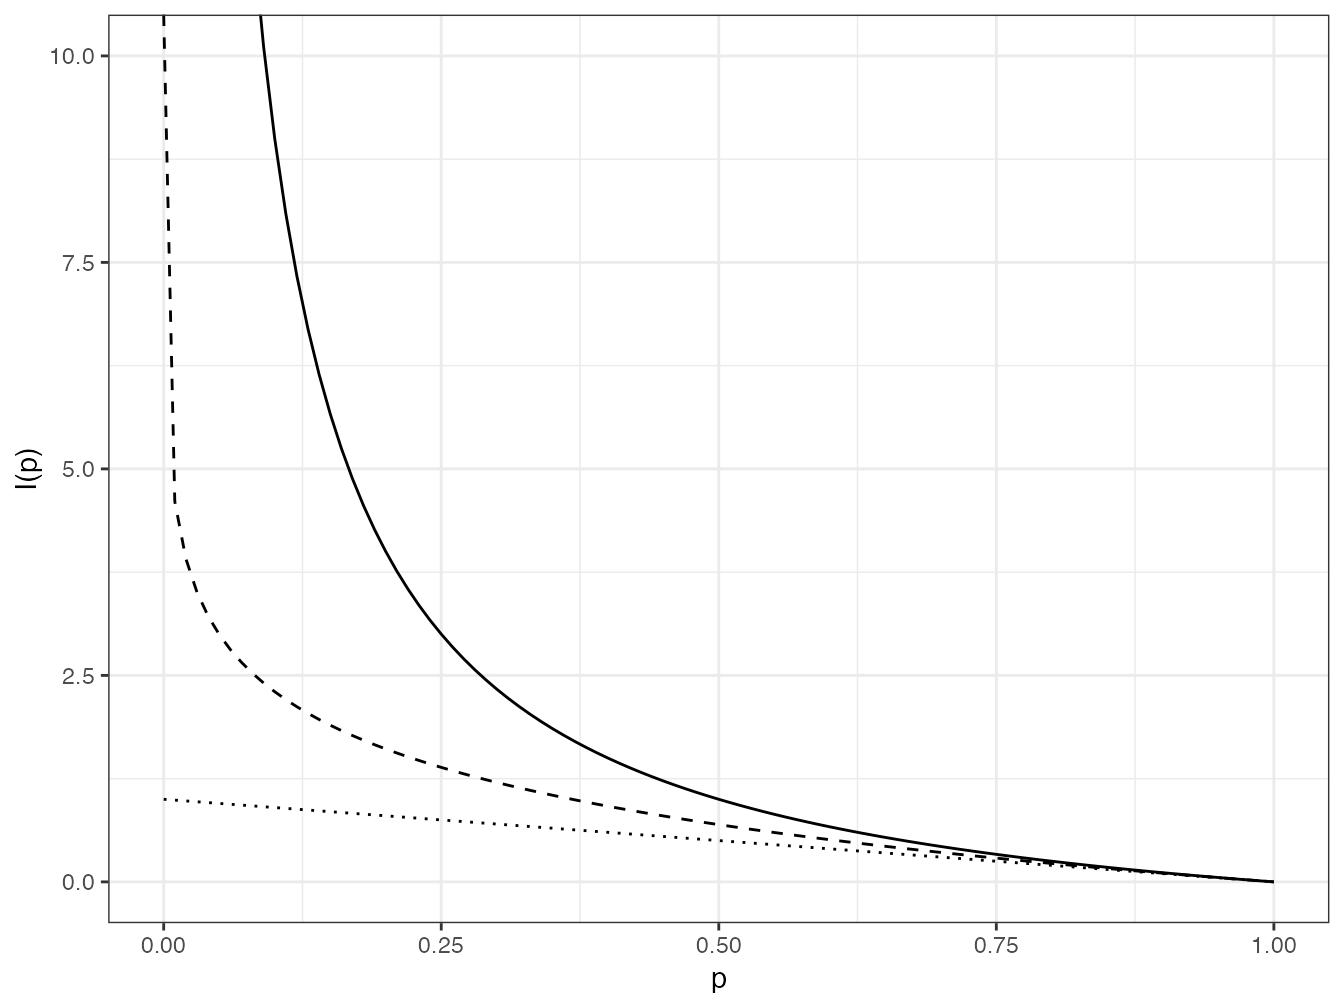
\includegraphics[width=0.8\linewidth]{MesuresBD_files/figure-latex/IFig-1} 

}

\caption{Fonctions d'information utilisées dans le nombre d'espèces (trait plein), l'indice de Shannon (pointillés longs) et l'indice de Simpson (pointillés). L'information apportée par l'observation d'espèces rares décroît du nombre d'espèces à l'indice de Simpson.}\label{fig:IFig}
\end{SCfigure}

\normalsize

Ces trois fonctions d'information sont représentées en figure \ref{fig:IFig}.

Le code R nécessaire pour réaliser la figure est:

\scriptsize

\begin{Shaded}
\begin{Highlighting}[]
\NormalTok{I0 <-}\StringTok{ }\ControlFlowTok{function}\NormalTok{(p) (}\DecValTok{1} \OperatorTok{-}\StringTok{ }\NormalTok{p)}\OperatorTok{/}\NormalTok{p}
\NormalTok{I1 <-}\StringTok{ }\ControlFlowTok{function}\NormalTok{(p) }\OperatorTok{-}\KeywordTok{log}\NormalTok{(p)}
\NormalTok{I2 <-}\StringTok{ }\ControlFlowTok{function}\NormalTok{(p) }\DecValTok{1} \OperatorTok{-}\StringTok{ }\NormalTok{p}
\KeywordTok{ggplot}\NormalTok{(}\KeywordTok{data.frame}\NormalTok{(}\DataTypeTok{x =} \KeywordTok{c}\NormalTok{(}\DecValTok{0}\NormalTok{, }\DecValTok{1}\NormalTok{)), }\KeywordTok{aes}\NormalTok{(x)) }\OperatorTok{+}\StringTok{ }\KeywordTok{stat_function}\NormalTok{(}\DataTypeTok{fun =}\NormalTok{ I0) }\OperatorTok{+}\StringTok{ }
\StringTok{    }\KeywordTok{stat_function}\NormalTok{(}\DataTypeTok{fun =}\NormalTok{ I1, }\DataTypeTok{lty =} \DecValTok{2}\NormalTok{) }\OperatorTok{+}\StringTok{ }\KeywordTok{stat_function}\NormalTok{(}\DataTypeTok{fun =}\NormalTok{ I2, }
    \DataTypeTok{lty =} \DecValTok{3}\NormalTok{) }\OperatorTok{+}\StringTok{ }\KeywordTok{coord_cartesian}\NormalTok{(}\DataTypeTok{ylim =} \KeywordTok{c}\NormalTok{(}\DecValTok{0}\NormalTok{, }\DecValTok{10}\NormalTok{)) }\OperatorTok{+}\StringTok{ }\KeywordTok{labs}\NormalTok{(}\DataTypeTok{x =} \StringTok{"p"}\NormalTok{, }
    \DataTypeTok{y =} \StringTok{"I(p)"}\NormalTok{)}
\end{Highlighting}
\end{Shaded}

\normalsize



\scriptsize

\begin{SCfigure}

{\centering 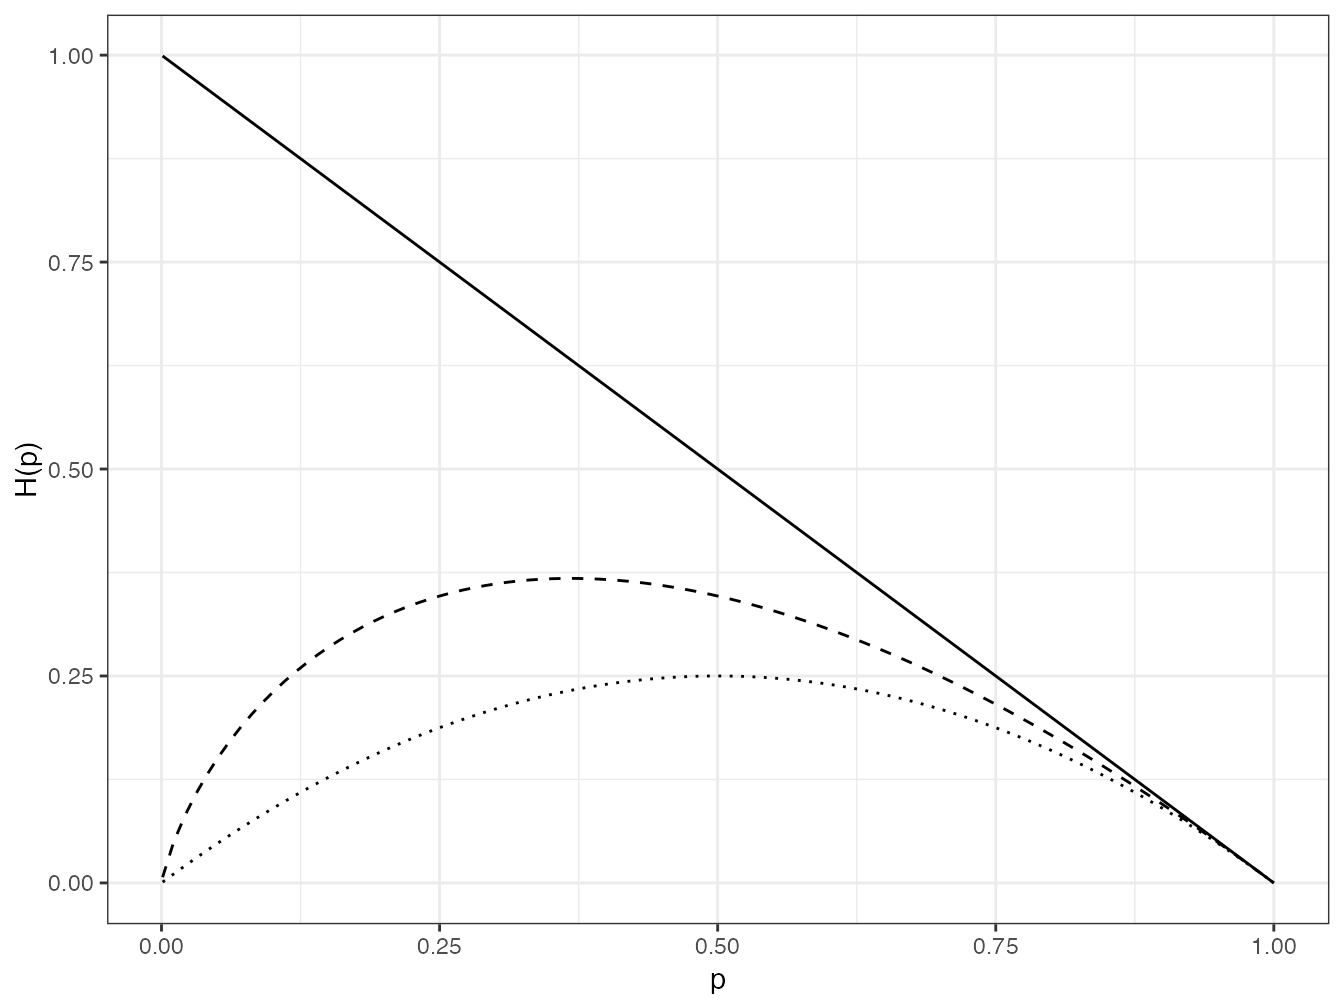
\includegraphics[width=0.8\linewidth]{MesuresBD_files/figure-latex/EntropieFig-1} 

}

\caption{Valeur de \(p_{s}I(p_s)\) dans le nombre d'espèces (trait plein), l'indice de Shannon (pointillés longs) et l'indice de Simpson (pointillés). Les espèces rares contribuent peu, sauf pour le nombre d'espèces.}\label{fig:EntropieFig}
\end{SCfigure}

\normalsize

La contribution de chaque espèce à la valeur totale de l'entropie est représentée figure \ref{fig:EntropieFig}.

Code R:

\scriptsize

\begin{Shaded}
\begin{Highlighting}[]
\NormalTok{H0 <-}\StringTok{ }\ControlFlowTok{function}\NormalTok{(p) }\DecValTok{1} \OperatorTok{-}\StringTok{ }\NormalTok{p}
\NormalTok{H1 <-}\StringTok{ }\ControlFlowTok{function}\NormalTok{(p) }\OperatorTok{-}\NormalTok{p }\OperatorTok{*}\StringTok{ }\KeywordTok{log}\NormalTok{(p)}
\NormalTok{H2 <-}\StringTok{ }\ControlFlowTok{function}\NormalTok{(p) p }\OperatorTok{*}\StringTok{ }\NormalTok{(}\DecValTok{1} \OperatorTok{-}\StringTok{ }\NormalTok{p)}
\KeywordTok{ggplot}\NormalTok{(}\KeywordTok{data.frame}\NormalTok{(}\DataTypeTok{x =} \KeywordTok{c}\NormalTok{(}\FloatTok{0.001}\NormalTok{, }\DecValTok{1}\NormalTok{)), }\KeywordTok{aes}\NormalTok{(x)) }\OperatorTok{+}\StringTok{ }\KeywordTok{stat_function}\NormalTok{(}\DataTypeTok{fun =}\NormalTok{ H0) }\OperatorTok{+}\StringTok{ }
\StringTok{    }\KeywordTok{stat_function}\NormalTok{(}\DataTypeTok{fun =}\NormalTok{ H1, }\DataTypeTok{lty =} \DecValTok{2}\NormalTok{) }\OperatorTok{+}\StringTok{ }\KeywordTok{stat_function}\NormalTok{(}\DataTypeTok{fun =}\NormalTok{ H2, }
    \DataTypeTok{lty =} \DecValTok{3}\NormalTok{) }\OperatorTok{+}\StringTok{ }\KeywordTok{labs}\NormalTok{(}\DataTypeTok{x =} \StringTok{"p"}\NormalTok{, }\DataTypeTok{y =} \StringTok{"H(p)"}\NormalTok{)}
\end{Highlighting}
\end{Shaded}

\normalsize

\hypertarget{entropie-relative}{%
\section{Entropie relative}\label{entropie-relative}}

Considérons maintenant les probabilités \(q_s\) formant l'ensemble \(\mathbf{q}\) obtenues par la réalisation de l'expérience.
Elles sont différentes des probabilités \(p_s\), par exemple parce que l'expérience ne s'est pas déroulée exactement comme prévu.
On définit le gain d'information \(I(q_s,p_s)\) comme la quantité d'information supplémentaire fournie par l'observation d'un résultat de l'expérience, connaissant les probabilités \emph{a priori}.
La quantité totale d'information fournie par l'expérience, \(\sum^S_{s=1}{q_sI(q_s,p_s)}=H(\mathbf{q},\mathbf{p})\), est souvent appelée entropie relative.
Elle peut être vue comme une distance entre la distribution \emph{a priori} et la distribution \emph{a posteriori}.
Il est possible que les distributions \(\mathbf{p}\) et \(\mathbf{q}\) soit identiques, que le gain d'information soit donc nul, mais les estimateurs empiriques n'étant pas exactement égaux entre eux, des tests de significativité de la valeur de \(\hat{H}(\mathbf{q},\mathbf{p})\) seront nécessaires.

Quelques formes possibles de \(H(\mathbf{q},\mathbf{p})\) sont:

\begin{itemize}
\tightlist
\item
  La divergence de Kullback-Leibler \autocite{Kullback1951} connue par les économistes comme l'indice de dissimilarité de \textcite{Theil1967}:
  \begin{equation}
  \label{eq:Theil}
  T = \sum^S_{s=1}{q_{s}\ln\frac{q_s}{p_s}};
  \end{equation}
\item
  Sa proche parente, appelée parfois deuxième mesure de Theil \autocite{Conceicao2000}, qui inverse simplement les rôles de \(p\) et \(q\):
  \begin{equation}
  \label{eq:Theil2}
  L = \sum^S_{s=1}{p_{s}\ln\frac{p_s}{q_s}}.
  \end{equation}
\end{itemize}



\scriptsize

\begin{SCfigure}

{\centering 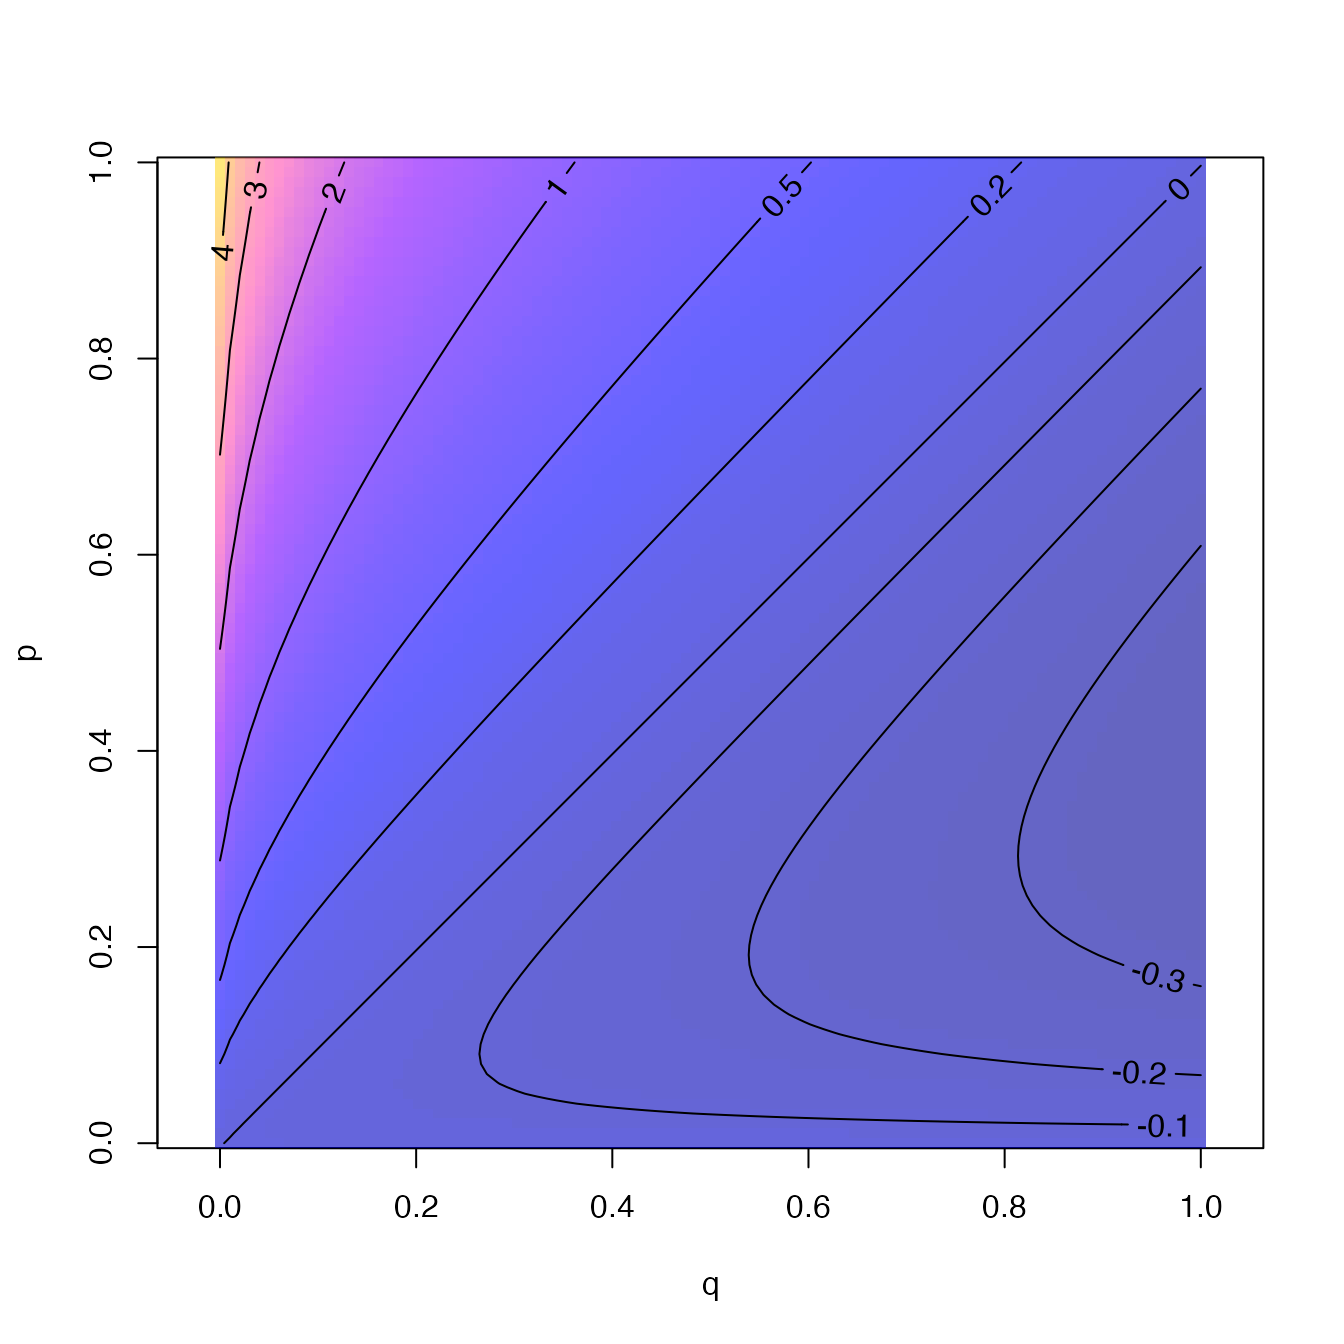
\includegraphics[width=0.8\linewidth]{MesuresBD_files/figure-latex/KullbackLeiblerFig-1} 

}

\caption{Valeur de \(q\ln(q/p)\) en fonction de \(p\) et \(q\). La divergence de Kullback-Leibler est la somme de cette valeur pour toutes les espèces}\label{fig:KullbackLeiblerFig}
\end{SCfigure}

\normalsize

L'entropie relative est essentielle pour la définition de la diversité \(\beta\) présentée dans le chapitre \ref{chap:DedompHCDT}.
En se limitant à la diversité \(\alpha\), on peut remarquer que l'indice de Shannon est la divergence de Kullback-Leibler entre la distribution observée et l'équiprobabilité des espèces \autocite{Marcon2012a}.
Les valeurs de chaque terme de la divergence sont représentées en figure \ref{fig:KullbackLeiblerFig}.

Le code R nécessaire pour réaliser la figure est:

\scriptsize

\begin{Shaded}
\begin{Highlighting}[]
\NormalTok{p <-}\StringTok{ }\NormalTok{q <-}\StringTok{ }\KeywordTok{seq}\NormalTok{(}\FloatTok{0.01}\NormalTok{, }\DecValTok{1}\NormalTok{, }\FloatTok{0.01}\NormalTok{)}
\NormalTok{KB <-}\StringTok{ }\ControlFlowTok{function}\NormalTok{(p, q) p }\OperatorTok{*}\StringTok{ }\KeywordTok{log}\NormalTok{(p}\OperatorTok{/}\NormalTok{q)}
\NormalTok{xyz <-}\StringTok{ }\KeywordTok{t}\NormalTok{(}\KeywordTok{outer}\NormalTok{(p, q, }\DataTypeTok{FUN =} \StringTok{"KB"}\NormalTok{))}
\KeywordTok{library}\NormalTok{(}\StringTok{"sp"}\NormalTok{)}
\KeywordTok{image}\NormalTok{(xyz, }\DataTypeTok{col =} \KeywordTok{bpy.colors}\NormalTok{(}\DataTypeTok{n =} \DecValTok{100}\NormalTok{, }\DataTypeTok{cutoff.tails =} \FloatTok{0.3}\NormalTok{, }\DataTypeTok{alpha =} \FloatTok{0.6}\NormalTok{), }
    \DataTypeTok{xlab =} \StringTok{"q"}\NormalTok{, }\DataTypeTok{ylab =} \StringTok{"p"}\NormalTok{, }\DataTypeTok{asp =} \DecValTok{1}\NormalTok{)}
\KeywordTok{contour}\NormalTok{(xyz, }\DataTypeTok{levels =} \KeywordTok{c}\NormalTok{(}\KeywordTok{seq}\NormalTok{(}\OperatorTok{-}\FloatTok{0.3}\NormalTok{, }\DecValTok{0}\NormalTok{, }\FloatTok{0.1}\NormalTok{), }\KeywordTok{c}\NormalTok{(}\FloatTok{0.2}\NormalTok{, }\FloatTok{0.5}\NormalTok{), }\KeywordTok{seq}\NormalTok{(}\DecValTok{1}\NormalTok{, }
    \DecValTok{4}\NormalTok{, }\DecValTok{1}\NormalTok{)), }\DataTypeTok{labcex =} \DecValTok{1}\NormalTok{, }\DataTypeTok{add =}\NormalTok{ T)}
\end{Highlighting}
\end{Shaded}

\normalsize

\hypertarget{lappropriation-de-lentropie-par-la-biodiversituxe9}{%
\section{L'appropriation de l'entropie par la biodiversité}\label{lappropriation-de-lentropie-par-la-biodiversituxe9}}

\textcite{MacArthur1955} est le premier à avoir introduit la théorie de l'information en écologie \autocite{Ulanowicz2001}.
MacArthur s'intéressait aux réseaux trophiques et cherchait à mesurer leur stabilité: l'indice de Shannon qui comptabilise le nombre de relations possibles lui paraissait une bonne façon de l'évaluer.
Mais l'efficacité implique la spécialisation, ignorée dans \(H\) qui est une mesure neutre (toutes les espèces y jouent le même rôle).
MacArthur a abandonné cette voie.

Les premiers travaux consistant à généraliser l'indice de Shannon sont dus à \textcite{Renyi1961}.
L'entropie d'ordre \(q\) de Rényi est

\begin{equation}
^{q}\!R =\frac{1}{1-q\ln\sum^S_{q=1}{p^q_s}}.
\end{equation}

Rényi pose également les axiomes pour une mesure d'entropie \(R\left(\mathbf{p}\right)\), où \(\mathbf{p}=(p_1,p_2,\dots,p_S)\):

\begin{itemize}
\tightlist
\item
  La symétrie: les espèces doivent être interchangeables, aucune n'a de rôle particulier et leur ordre est indifférent;
\item
  La mesure doit être continue par rapport aux probabilités;
\item
  La valeur maximale est atteinte si toutes les probabilités sont égales.
\end{itemize}

Il montre que \(^{q}\!R\) respecte les 3 axiomes.

\textcite{Patil1982} ont montré de plus que:

\begin{itemize}
\tightlist
\item
  L'introduction d'une espèce dans une communauté augmente sa diversité (conséquence de la décroissance de \(g(p_s)\));
\item
  Le remplacement d'un individu d'une espèce fréquente par un individu d'une espèce plus rare augmente l'entropie à condition que \(R(\mathbf{p})\) soit concave.
  Dans la littérature économique sur les inégalités, cette propriété est connue sous le nom de Pigou-Dalton \autocite{Dalton1920}.
\end{itemize}

\textcite{Hill1973} transforme l'entropie de Rényi en \emph{nombres de Hill}, qui en sont simplement l'exponentielle:

\begin{equation}
  \label{eq:Hill1973}
  ^{q}\!D = {\left(\sum^S_{s=1}{p^q_s}\right)}^{\frac{1}{1-q}}.
\end{equation}

Le souci de Hill était de rendre les indices de diversité intelligibles après l'article remarqué de \textcite{Hurlbert1971} intitulé ``le non-concept de diversité spécifique''.
Hurlbert reprochait à la littérature sur la diversité sa trop grande abstraction et son éloignement des réalités biologiques, notamment en fournissant des exemples dans lesquels l'ordre des communautés n'est pas le même selon l'indice de diversité choisi.
Les nombres de Hill sont le nombre d'espèces équiprobables donnant la même valeur de diversité que la distribution observée.
Ils sont des transformations simples des indices classiques:

\begin{itemize}
\tightlist
\item
  \(^{0}\!D\) est le nombre d'espèces;
\item
  \(^{1}\!D=e^H\), l'exponentielle de l'indice de Shannon;
\item
  \(^{2}\!D={1}/{\left(1-E\right)}\), l'inverse de l'indice de concentration de Simpson, connu sous le nom d'indice de \textcite{Stoddart1983}.
\end{itemize}

Ces résultats avaient déjà été obtenus avec une autre approche par \textcite{MacArthur1965} et repris par \textcite{Adelman1969} dans la littérature économique.

Les nombres de Hill sont des ``nombres effectifs'' ou ``nombres équivalents''.
Le concept a été défini rigoureusement par \textcite{Gregorius1991}, d'après \textcite{Wright1931} (qui avait le premier défini la taille effective d'une population): étant donné une variable caractéristique (ici, l'entropie) fonction seulement d'une variable numérique (ici, le nombre d'espèces) dans un cas idéal (ici, l'équiprobabilité des espèces), le nombre effectif est la valeur de la variable numérique pour laquelle la variable caractéristique est celle du jeu de données.

\textcite{Gregorius2014} montre que de nombreux autres indices de diversité sont acceptables dans le sens où ils vérifient les axiomes précédents et, de plus, que la diversité d'un assemblage de communautés est obligatoirement supérieure à la diversité moyenne de ces communautés (l'égalité n'étant possible que si les communautés sont toutes identiques).
Cette dernière propriété sera traitée en détail dans la partie consacrée à la décomposition de la diversité.
Ces indices doivent vérifier deux propriétés: leur fonction d'information doit être décroissante, et ils doivent être une fonction strictement concave de \(p_s\).
Parmi les possibilités, \(I(p_s) = \cos{(p_s {\pi}/{2})}\) est envisageable par exemple: le choix de la fonction d'information est virtuellement illimité, mais seules quelques unes seront interprétables clairement.

Un nombre équivalent d'espèces existe pour tous ces indices, il est toujours égal à l'inverse de l'image de l'indice par la réciproque de la fonction d'information:

\begin{equation}
  \label{eq:Gregorius2014}
  D = \frac{1}{I^{-1}\left(\sum^S_{s=1}{p_s I(p_s)}\right)}.
\end{equation}

D'autres entropies ont été utlisées, avec plus ou moins de succès.
Par exemple, \textcite{Ricotta2003c} proposent d'utiliser la fonction d'information \(I(p_s)=-\ln(k_s)\) où \(k_s\) est la dissimilarité totale de l'espèce \(s\) avec les autres (par exemple, la somme des distances aux autres espèces dans un arbre phylogénétique, voir section \ref{sec:Dphylo}), normalisée pour que \(\sum_s{k_s}=1\).
Ainsi, les espèces les plus originales apportent peu d'information, ce qui n'est pas très intuitif.
Les auteurs montrent que leur mesure est la somme de l'entropie de Shannon et de la divergence de Kullback-Leibler entre les probabilités et les dissimilarités des espèces.
\textcite{Ricotta2006b} ont défini plus tard une entropie augmentant avec l'originalité de chaque espèce, présentée au chapitre \ref{chap:LeinsterCobbold}.

\hypertarget{entropie-hcdt}{%
\section{Entropie HCDT}\label{entropie-hcdt}}

\textcite{Tsallis1988} propose une classe de mesures appelée entropie généralisée, définie par \textcite{Havrda1967} pour la première fois et redécouverte plusieurs fois, notamment par \textcite{Daroczy1970}, d'où son nom \emph{entropie HCDT} (voir \textcite{Mendes2008}, page 451, pour un historique complet):

\begin{equation}
  \label{eq:HCDT}
  ^{q}\!H = \frac{1}{q-1}\left(1-\sum^S_{s=1}{p^q_s}\right).
\end{equation}

Tsallis a montré que les indices de Simpson et de Shannon étaient des cas particuliers d'entropie généralisée, retrouvant, sans faire le rapprochement \autocite{Ricotta2005}, la définition d'un indice de diversité de \textcite{Patil1982}.

Ces résultats ont été complétés par d'autres et repris en écologie par \textcite{Keylock2005} et Jost (\autocite*{Jost2006}; \autocite*{Jost2007}).
Là encore:

\begin{itemize}
\tightlist
\item
  Le nombre d'espèces moins 1 est \(^{0}\!H\);
\item
  L'indice de Shannon est \(^{1}\!H\);
\item
  L'indice de Gini-Simpson est \(^{2}\!H\).
\end{itemize}

L'entropie HCDT est particulièrement attractive parce que sa relation avec la diversité au sens strict est simple, après introduction du formalisme adapté (les logarithmes déformés).
Son biais d'estimation peut être corrigé globalement, et non seulement pour les cas particuliers (nombre d'espèces, Shannon, Simpson).
Enfin, sa décomposition sera présentée en détail dans le chapitre \ref{chap:DedompHCDT}.

\hypertarget{logarithmes-duxe9formuxe9s}{%
\subsection{Logarithmes déformés}\label{logarithmes-duxe9formuxe9s}}

L'écriture de l'entropie HCDT est largement simplifiée en introduisant le formalisme des logarithmes déformés \autocite{Tsallis1994}.
Le logarithme d'ordre \(q\) est défini par
\begin{equation}
  \label{eq:lnq}
  \ln_q{x} = \frac{x^{1-q}-1}{1-q},
\end{equation}
dont la forme est identique à la transformation de \textcite{Box1964} utilisée en statistiques pour normaliser une variable.

Le logarithme déformé converge vers le logarithme naturel quand \(q\to 1\) (figure \ref{fig:lnqFig}).

Le code R nécessaire pour réaliser la figure est:

\scriptsize

\begin{Shaded}
\begin{Highlighting}[]
\NormalTok{ln0 <-}\StringTok{ }\ControlFlowTok{function}\NormalTok{(p) }\KeywordTok{lnq}\NormalTok{(p, }\DecValTok{0}\NormalTok{)}
\NormalTok{ln2 <-}\StringTok{ }\ControlFlowTok{function}\NormalTok{(p) }\KeywordTok{lnq}\NormalTok{(p, }\DecValTok{2}\NormalTok{)}
\NormalTok{lnm1 <-}\StringTok{ }\ControlFlowTok{function}\NormalTok{(p) }\KeywordTok{lnq}\NormalTok{(p, }\DecValTok{-1}\NormalTok{)}
\KeywordTok{ggplot}\NormalTok{(}\KeywordTok{data.frame}\NormalTok{(}\DataTypeTok{x =} \KeywordTok{c}\NormalTok{(}\DecValTok{0}\NormalTok{, }\DecValTok{1}\NormalTok{)), }\KeywordTok{aes}\NormalTok{(x)) }\OperatorTok{+}\StringTok{ }
\StringTok{    }\KeywordTok{stat_function}\NormalTok{(}\DataTypeTok{fun =}\NormalTok{ log) }\OperatorTok{+}
\StringTok{    }\KeywordTok{stat_function}\NormalTok{(}\DataTypeTok{fun =}\NormalTok{ ln0, }\DataTypeTok{lty =} \DecValTok{2}\NormalTok{, }\DataTypeTok{col =} \StringTok{"red"}\NormalTok{) }\OperatorTok{+}
\StringTok{    }\KeywordTok{stat_function}\NormalTok{(}\DataTypeTok{fun =}\NormalTok{ ln2, }\DataTypeTok{lty =} \DecValTok{3}\NormalTok{, }\DataTypeTok{col =} \StringTok{"blue"}\NormalTok{) }\OperatorTok{+}
\StringTok{    }\KeywordTok{stat_function}\NormalTok{(}\DataTypeTok{fun =}\NormalTok{ lnm1, }\DataTypeTok{lty =} \DecValTok{4}\NormalTok{, }\DataTypeTok{col =} \StringTok{"green"}\NormalTok{) }\OperatorTok{+}
\StringTok{    }\KeywordTok{coord_cartesian}\NormalTok{(}\DataTypeTok{ylim =} \KeywordTok{c}\NormalTok{(}\OperatorTok{-}\DecValTok{4}\NormalTok{, }\DecValTok{0}\NormalTok{)) }\OperatorTok{+}
\StringTok{    }\KeywordTok{labs}\NormalTok{(}\DataTypeTok{x =} \StringTok{"p"}\NormalTok{, }\DataTypeTok{y =} \KeywordTok{expression}\NormalTok{(ln[q](p)))}
\end{Highlighting}
\end{Shaded}

\normalsize

Sa fonction inverse est l'exponentielle d'ordre \(q\):

\begin{equation}
  \label{eq:expq}
  e^x_q = \left[ 1+\left( 1-q \right)x \right]^{\frac{1}{1-q}}.
\end{equation}



\scriptsize

\begin{SCfigure}

{\centering 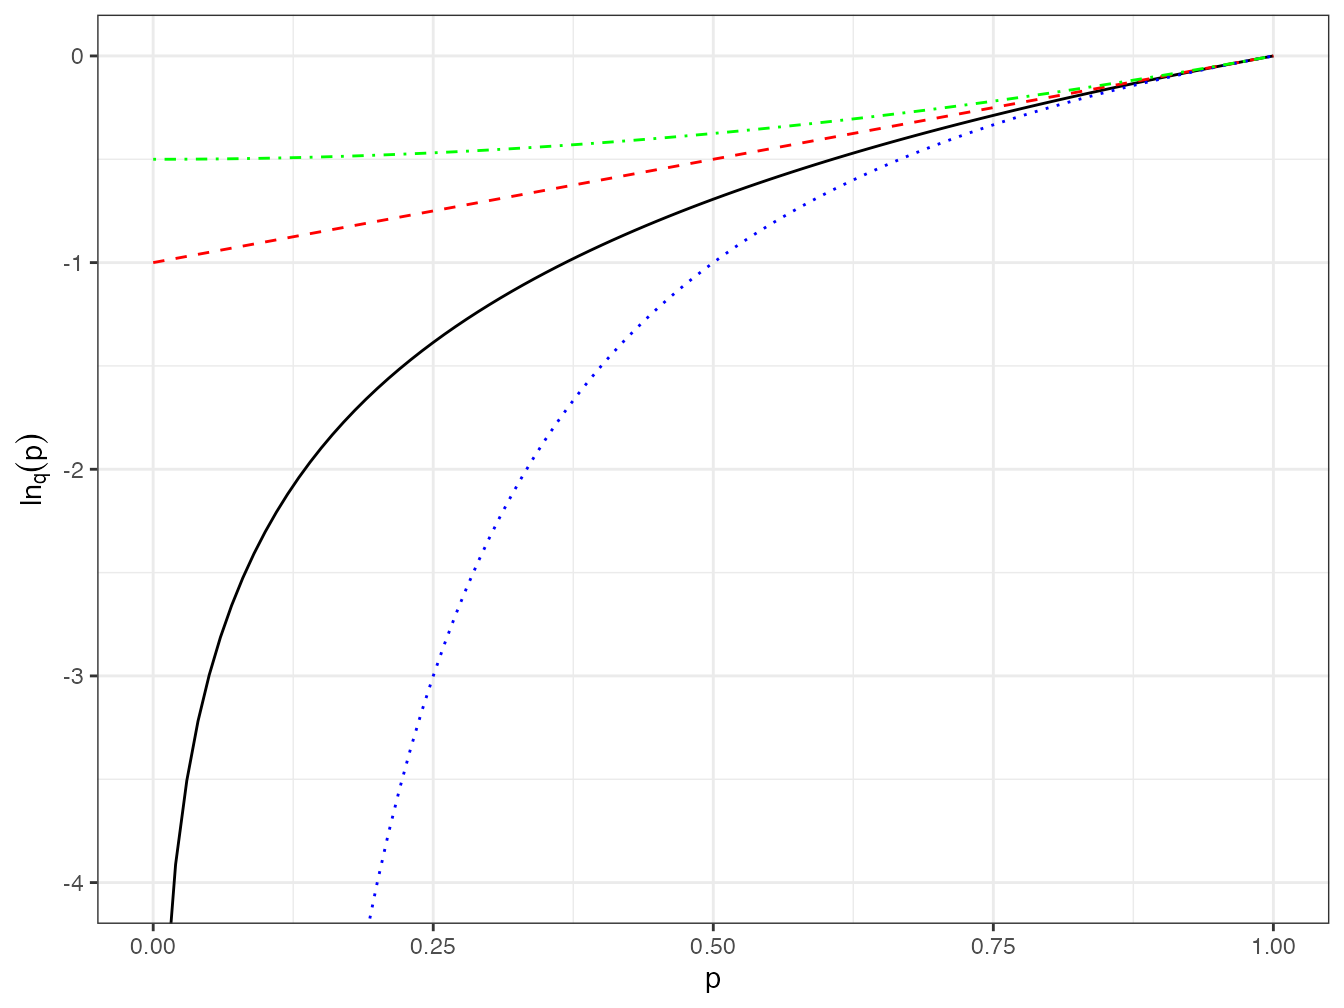
\includegraphics[width=0.8\linewidth]{MesuresBD_files/figure-latex/lnqFig-1} 

}

\caption{Valeur du logarithme d'ordre \(q\) de probabilités entre 0 et 1 pour différentes valeurs de \(q\): \(q = 0\) (pointillés longs rouges), la courbe est une droite; \(q = 1\) (trait plein): logarithme naturel; \(q = 2\) (pointillés courts bleus): la courbe a la même forme que le logarithme naturel pour les valeurs positives de \(q\); \(q =-1\) (pointillés alternés verts): la courbe est convexe pour les valeurs négatives de \(q\).}\label{fig:lnqFig}
\end{SCfigure}

\normalsize

Enfin, le logarithme déformé est subadditif:

\begin{equation}
  \label{eq:lnqsubadd}
  \ln_q\left(xy\right)=\ln_q{x}+\ln_q{y}-\left(q-1\right)\left(\ln_q{x}\right)\left(\ln_q{y}\right).
\end{equation}

Ses propriétés sont les suivantes:

\begin{equation}
  \label{eq:lnqinv}
  \ln_q\frac{1}{x}=-x^{q-1}\ln_qx;
\end{equation}

\begin{equation}
  \label{eq:lnqprod}
  \ln_q\left(xy\right)=\ln_q{x}+x^{1-q}\ln_q{y};
\end{equation}

\begin{equation}
  \label{eq:lnqdiv}
  \ln_q\left(\frac{x}{y}\right)=\ln_q{x}-{\left(\frac{x}{y}\right)}^{1-q}\ln_q{y};
\end{equation}

et

\begin{equation}
  \label{eq:expqsum}
  e^{x+y}_q = e_q^x e^{\frac{y}{1+\left(1-q\right)x}}_q.
\end{equation}

Si \(q>1\), \({\mathop{\lim}_{x\to +\infty} \left(\ln_q{x}\right)={1}/{\left(q-1\right)}}\), donc \(e^x_q\) n'est pas définie pour \(x>{1}/{\left(q-1\right)}\).

La dérivée du logarithme déformé est, quel que soit \(q\),
\begin{equation}
  \label{eq:lnqprime}
  \ln'_q\left(x\right) = x^{-q}.
\end{equation}

Les dérivées première et seconde de l'exponentielle déformée sont, quel que soit \(q\):
\begin{equation}
  \label{eq:expqprime}
  \exp'_q\left(x\right) = \left( e_q^x \right)^{q};
\end{equation}
\begin{equation}
  \label{eq:expqsec}
  \exp''_q\left(x\right) = \left( e_q^x \right)^{2q-1}.
\end{equation}

Ces fonctions sont implémentées dans le package \emph{entropart}: \texttt{lnq(x,\ q)} et \texttt{expq(x,\ q)}.

L'entropie d'ordre \(q\) s'écrit

\begin{equation}
  \label{eq:EntropieHCDT}
  ^{q}\!H = \frac{1}{q-1}\left(1-\sum^S_{s=1}{p^q_s}\right)=-\sum_s{p^q_s}\ln_q{p_s}=\sum_s{p_s}\ln_q\frac{1}{p_s}.
\end{equation}

Ces trois formes sont équivalentes mais les deux dernières s'interprètent comme une généralisation de l'entropie de Shannon \autocite{Marcon2014a}.

Le calcul de \(^{q}\!H\) peut se faire avec la fonction \texttt{Tsallis} de la librairie \emph{entropart}:

\scriptsize

\begin{Shaded}
\begin{Highlighting}[]
\NormalTok{Ps <-}\StringTok{ }\KeywordTok{as.ProbaVector}\NormalTok{(}\KeywordTok{colSums}\NormalTok{(BCI))}
\NormalTok{q <-}\StringTok{ }\FloatTok{1.5}
\KeywordTok{Tsallis}\NormalTok{(Ps, q)}
\end{Highlighting}
\end{Shaded}

\begin{verbatim}
##     None 
## 1.715954
\end{verbatim}

\normalsize

\hypertarget{entropie-et-diversituxe9}{%
\subsection{Entropie et diversité}\label{entropie-et-diversituxe9}}

On voit immédiatement que l'entropie de Tsallis est le logarithme d'ordre \(q\) du nombre de Hill correspondant, comme l'entropie de Rényi en est le logarithme naturel:

\begin{equation}
  \label{eq:HlnD}
  ^{q}\!H = \ln_q{^{q}\!D};
\end{equation}

\begin{equation}
  \label{eq:DexpH}
  ^{q}\!D = e_q^{^{q}\!H}.
\end{equation}

L'entropie est utile pour les calculs: la correction des biais d'estimation notamment.
Les nombres de Hill, ou \emph{nombres équivalents d'espèces} ou \emph{nombres effectif d'espèces} permettent une appréhension plus intuitive de la notion de biodiversité \autocite{Jost2006}.
En raison de leurs propriétés, notamment de décomposition (voir le chapitre \ref{chap:DedompHCDT}), \textcite{Jost2007} les appelle ``vraie diversité''.
\textcite{Hoffmann2008} critiquent cette définition totalitaire et fournissent une revue historique plus lointaine sur les origines de ces mesures.
\textcite{Jost2009} reconnaît qu'un autre terme aurait pu être choisi (``diversité neutre'' ou ``diversité mathématique'' par exemple).

\textcite{Dauby2012} écrivent ``diversité au sens strict''; \textcite{Gregorius2010} ``diversité explicite''.

Quoi qu'il en soit, les nombres de Hill respectent le principe de réplication (voir \textcite{Chao2010}, section 3 pour une discussion et un historique): si \(I\) communautés de même taille, de même niveau de diversité \(D\), mais sans espèces en commun sont regroupées dans une méta-communauté, la diversité de la méta-communauté doit être \(I\times D\).

L'intérêt de ces approches est de fournir une définition paramétrique de la diversité, qui donne plus ou moins d'importance aux espèces rares:

\begin{itemize}
\tightlist
\item
  \(^{-\infty}\!D={1}/{\min(p_S)}\) est l'inverse de la proportion de la communauté représentée par l'espèce la plus rare (toutes les autres espèces sont ignorées).
  Le biais d'estimation est incontrôlable: l'espèce la plus rare n'est pas dans l'échantillon tant que l'inventaire n'est pas exhaustif;
\item
  \(^{0}\!D\) est le nombre d'espèces (alors que \(^{0}\!H\) est le nombre d'espèces moins 1). C'est la mesure classique qui donne le plus d'importance aux espèces rares: toutes les espèces ont la même importance, quel que soit leur effectif en termes d'individus.
  Il est bien adapté à une approche patrimoniale, celle du collectionneur qui considère que l'existence d'une espèce supplémentaire a un intérêt en soi, par exemple parce qu'elle peut contenir une molécule valorisable.
  Comme les espèces rares sont difficiles à échantillonner, le biais d'estimation est très important, et sa résolution a généré une littérature en soi;
\item
  \(^{1}\!D\) est l'exponentielle de l'indice de Shannon donne la même importance à tous les individus.
  Il est adapté à une approche d'écologue, intéressé par les interactions possibles: le nombre de combinaisons d'espèces en est une approche satisfaisante.
  Le biais d'estimation est sensible;
\item
  \(^{2}\!D\) est l'inverse de l'indice de concentration de Gini-Simpson donne moins d'importance aux espèces rares.
  \textcite{Hill1973} l'appelle ``le nombre d'espèces très abondantes''.
  Il comptabilise les interactions possibles entre paires d'individus: les espèces rares interviennent dans peu de paires, et influent peu sur l'indice.
  En conséquence, le biais d'estimation est très petit; de plus, un estimateur non biaisé existe;
\item
  \(^{\infty}\!D={1}/{d}\) est l'inverse de l'indice de Berger-Parker \autocite{Berger1970} qui est la proportion de la communauté représentée par l'espèce la plus abondante: \(d=\max(\mathbf{p})\).
  Toutes les autres espèces sont ignorées.
\end{itemize}

Le calcul de \(^{q}\!D\) peut se faire avec la fonction \texttt{Diversity} de la librairie \emph{entropart}:

\scriptsize

\begin{Shaded}
\begin{Highlighting}[]
\NormalTok{Ps <-}\StringTok{ }\KeywordTok{as.ProbaVector}\NormalTok{(}\KeywordTok{colSums}\NormalTok{(BCI))}
\NormalTok{q <-}\StringTok{ }\FloatTok{1.5}
\KeywordTok{Diversity}\NormalTok{(Ps, q)}
\end{Highlighting}
\end{Shaded}

\begin{verbatim}
##     None 
## 49.57724
\end{verbatim}

\normalsize

Les propriétés mathématiques de la diversité ne sont pas celles de l'entropie.
L'entropie doit être une fonction concave des probabilités comme on l'a vu plus haut, mais pas la diversité (un exemple de confusion est fourni par \textcite{Gadagkar1989}, qui reproche à \(^{2}\!D\) de ne pas être concave).
L'entropie est une moyenne pondérée par les probabilités de la fonction d'information, c'est donc une fonction linéaire des probabilités, propriété importante pour définir l'entropie \(\alpha\) (section \ref{sec:defalpha}) comme la moyenne des entropies de plusieurs communautés, ou l'entropie phylogénétique (chapitre \ref{chap:Phyloentropie}) comme la moyenne de l'entropie sur les périodes d'un arbre.
La diversité n'est pas une fonction linéaire des probabilités: la diversité moyenne n'est en général pas la moyenne des diversités.

\hypertarget{synthuxe8se}{%
\subsection{Synthèse}\label{synthuxe8se}}

L'inverse de la probabilité d'une espèce, \(1/p_s\), définit sa rareté.
L'entropie est la moyenne du logarithme de la rareté:

\begin{equation}
  \label{eq:EntropieRarete}
  ^{q}\!H = \frac{1}{q-1}\left(1-\sum^S_{s=1}{p^q_s}\right)=\sum_s{p_s}\ln_q\frac{1}{p_s}.
\end{equation}

La diversité est son exponentielle:

\begin{equation}
  \label{eq:DexpHSynthese}
  ^{q}\!D = e_q^{^{q}\!H}.
\end{equation}

\hypertarget{profils-de-diversituxe9}{%
\section{Profils de diversité}\label{profils-de-diversituxe9}}

\textcite{Leinster2012}, après \textcite{Hill1973}, \textcite{Patil1982}, \textcite{Tothmeresz1995} et \textcite{Kindt2006}, recommandent de tracer des profils de diversité, c'est-à-dire la valeur de la diversité \(^{q}\!D\) en fonction de l'ordre \(q\) (figure \ref{fig:ProfilDivFig}) pour comparer plusieurs communautés.
Une communauté peut être déclarée plus diverse qu'une autre si son profil de diversité est au-dessus de l'autre pour toutes les valeurs de \(q\).
Si les courbes se croisent, il n'y a pas de relation d'ordre \autocite{Tothmeresz1995}.

\textcite{Lande2000} montrent que si la diversité de Simpson et la richesse de deux communautés n'ont pas le même ordre, alors les courbes d'accumulation du nombre d'espèces en fonction du nombre d'individus échantillonnés se croisent aussi.



\scriptsize

\begin{SCfigure}

{\centering 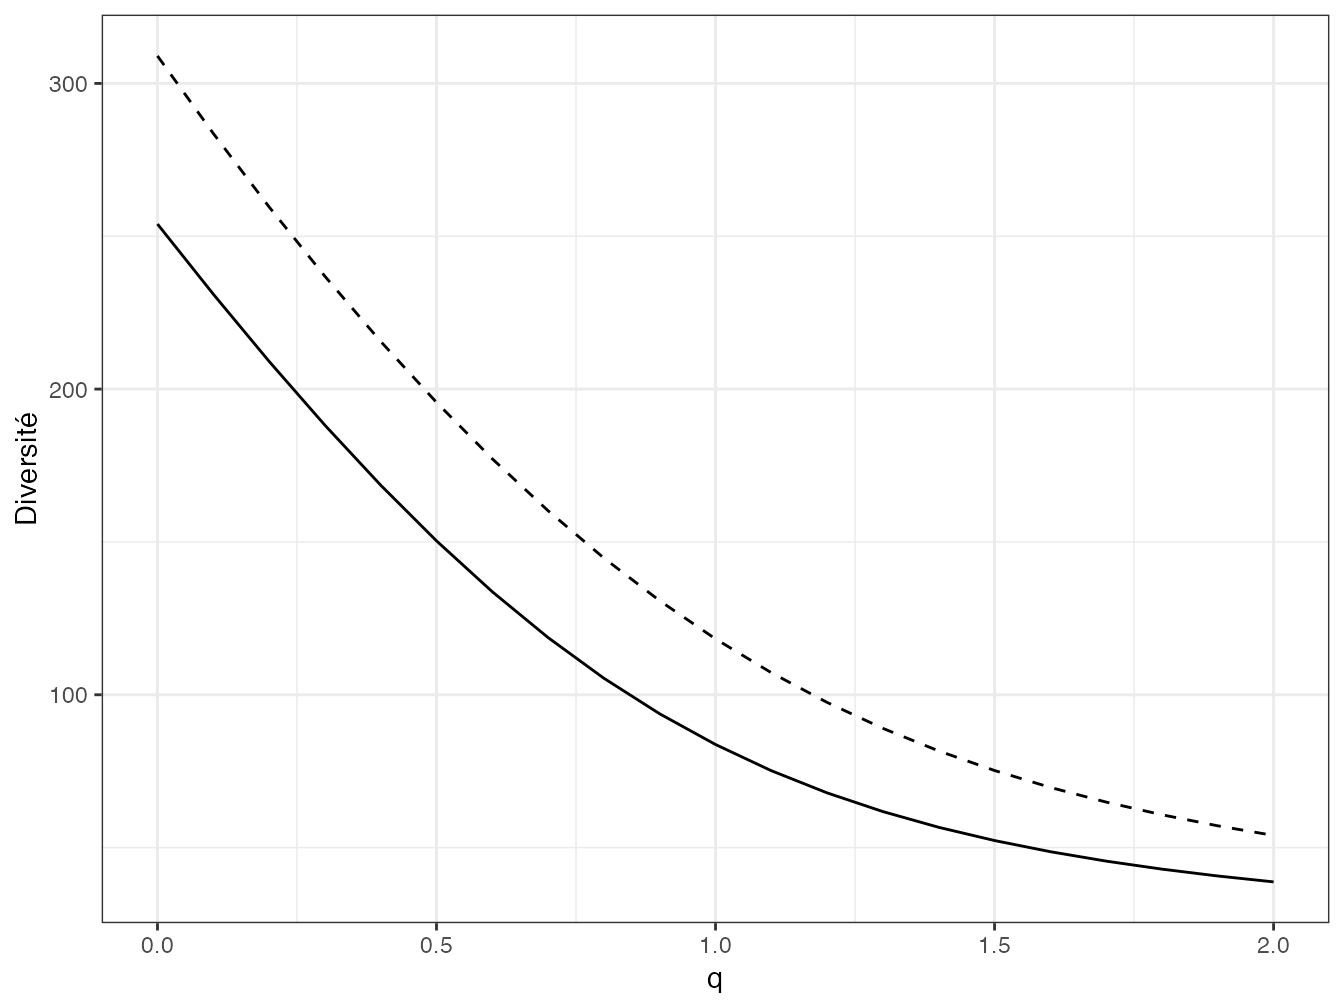
\includegraphics[width=0.8\linewidth]{MesuresBD_files/figure-latex/ProfilDivFig-1} 

}

\caption{Profil de diversité calculé pour deux parcelles de Paracou (Parcelle 6: trait plein et Parcelle 18: trait pointillé). La correction du biais d'estimation est celle de Chao et Jost.}\label{fig:ProfilDivFig}
\end{SCfigure}

\normalsize

Code R pour réaliser la figure \ref{fig:ProfilDivFig}:

\scriptsize

\begin{Shaded}
\begin{Highlighting}[]
\NormalTok{q.seq <-}\StringTok{ }\KeywordTok{seq}\NormalTok{(}\DecValTok{0}\NormalTok{, }\DecValTok{2}\NormalTok{, }\FloatTok{.1}\NormalTok{)}
\NormalTok{  P6D<-}\StringTok{ }\KeywordTok{CommunityProfile}\NormalTok{(Diversity, Paracou618.MC}\OperatorTok{$}\NormalTok{Nsi[, }\DecValTok{1}\NormalTok{], q.seq)}
\NormalTok{  P18D<-}\StringTok{ }\KeywordTok{CommunityProfile}\NormalTok{(Diversity, Paracou618.MC}\OperatorTok{$}\NormalTok{Nsi[, }\DecValTok{2}\NormalTok{], q.seq)}
  \KeywordTok{autoplot}\NormalTok{(P6D, }\DataTypeTok{xlab =} \StringTok{"q"}\NormalTok{, }\DataTypeTok{ylab =} \StringTok{"Diversité"}\NormalTok{) }\OperatorTok{+}
\StringTok{    }\KeywordTok{geom_line}\NormalTok{(}\KeywordTok{aes}\NormalTok{(x, y), }\KeywordTok{as.data.frame.list}\NormalTok{(P18D), }\DataTypeTok{lty =} \DecValTok{2}\NormalTok{)}
\end{Highlighting}
\end{Shaded}

\normalsize

\textcite{Pallmann2012} ont développé un test statistique pour comparer la diversité de deux communautés pour plusieurs valeurs de \(q\) simultanément.

\textcite{Liu2006} nomment \emph{séparables} des communautés dont les profils ne se croisent pas.
Ils montrent que des communautés peuvent être séparables en selon un profil de diversité de \(^{q}\!D\) sans l'être forcément selon un profil de diversité de Hurlbert (section \ref{sec:Hurlbert}), et inversement.
Ils montrent que les communautés séparables selon un troisième type de profil, celui de la queue de distribution \autocite{Patil1982}, le sont dans tous les cas.
Le profil de la queue de distribution est construit en classant les espèces de la plus fréquente à la plus rare et en traçant la probabilité qu'un individu appartienne à une espèce plus rare que l'espèce en abscisse (figure \ref{fig:ProfilQueueFig}).



\scriptsize

\begin{SCfigure}

{\centering 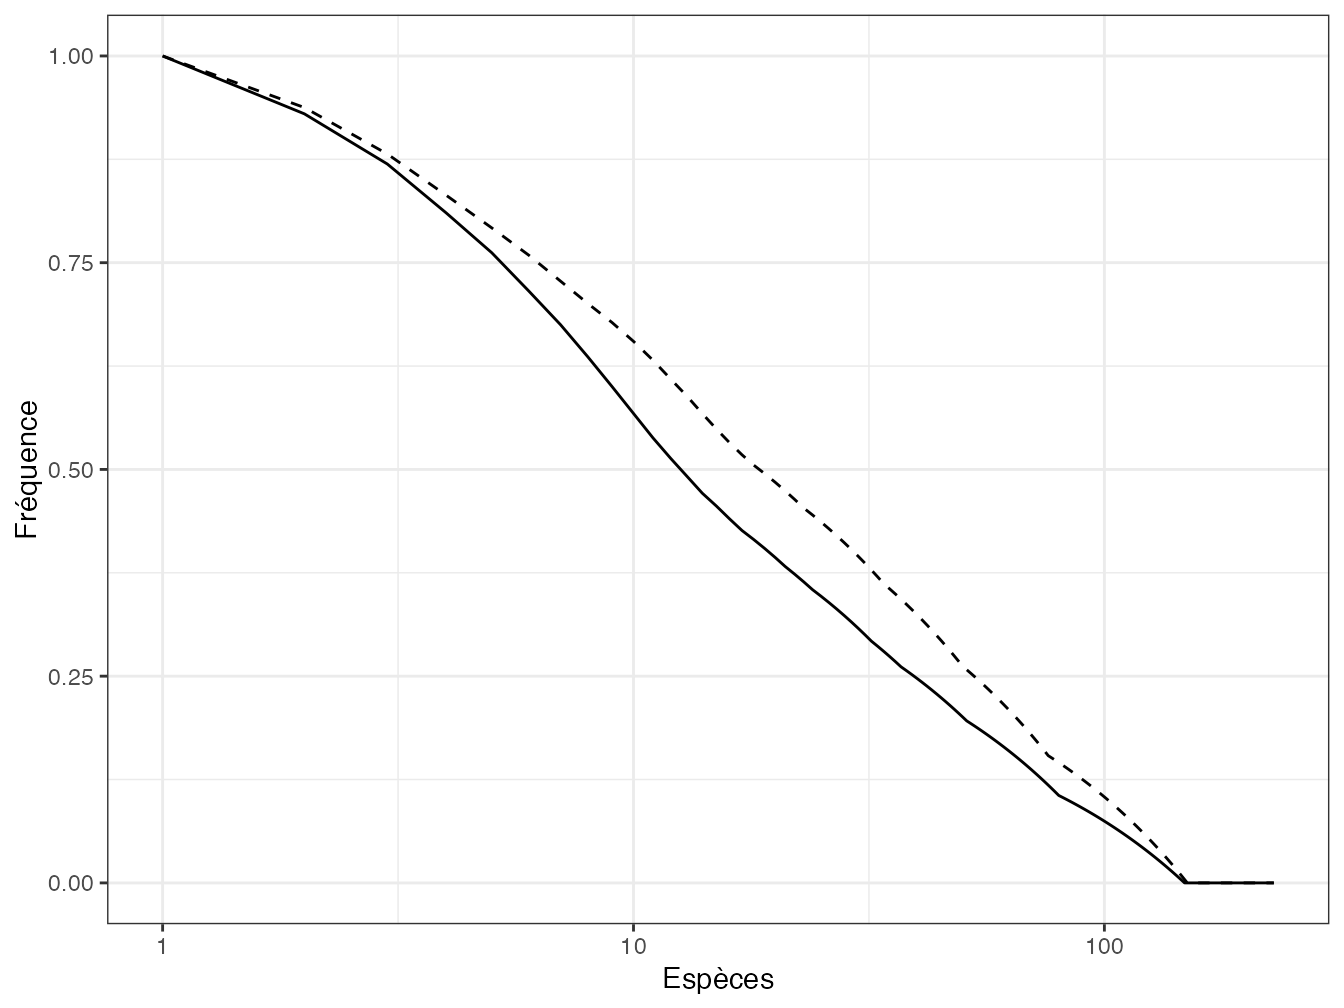
\includegraphics[width=0.8\linewidth]{MesuresBD_files/figure-latex/ProfilQueueFig-1} 

}

\caption{Profil de queue de distribution calculé pour les deux parcelles de Paracou (Parcelle 6: trait plein et Parcelle 18: trait pointillé). En abscisse: rang de l'espèce dans le classement de la plus fréquente à la plus rare; en ordonnée: probabilité qu'un individu de la communauté appartienne à une espèce plus rare.}\label{fig:ProfilQueueFig}
\end{SCfigure}

\normalsize

Code R:

\scriptsize

\begin{Shaded}
\begin{Highlighting}[]
\CommentTok{# Elimination des espèces absentes des deux parcelles}
\NormalTok{Psi <-}\StringTok{ }\KeywordTok{as.data.frame}\NormalTok{(Paracou618.MC}\OperatorTok{$}\NormalTok{Psi[Paracou618.MC}\OperatorTok{$}\NormalTok{Ps }\OperatorTok{>}\StringTok{ }\DecValTok{0}\NormalTok{, }
\NormalTok{    ])}
\NormalTok{Psi[, }\DecValTok{1}\NormalTok{] }\OperatorTok\StringTok{ }\NormalTok{sort }\OperatorTok\StringTok{ }\NormalTok{cumsum }\OperatorTok\StringTok{ }\NormalTok{rev}
\NormalTok{Psi[, }\DecValTok{2}\NormalTok{] }\OperatorTok\StringTok{ }\NormalTok{sort }\OperatorTok\StringTok{ }\NormalTok{cumsum }\OperatorTok\StringTok{ }\NormalTok{rev}
\NormalTok{Psi}\OperatorTok{$}\NormalTok{x <-}\StringTok{ }\DecValTok{1}\OperatorTok{:}\KeywordTok{nrow}\NormalTok{(Psi)}
\KeywordTok{ggplot}\NormalTok{(Psi, }\KeywordTok{aes}\NormalTok{(x)) }\OperatorTok{+}\StringTok{ }\KeywordTok{geom_path}\NormalTok{(}\KeywordTok{aes}\NormalTok{(}\DataTypeTok{y =}\NormalTok{ P006)) }\OperatorTok{+}\StringTok{ }\KeywordTok{geom_path}\NormalTok{(}\KeywordTok{aes}\NormalTok{(}\DataTypeTok{y =}\NormalTok{ P018), }
    \DataTypeTok{lty =} \DecValTok{2}\NormalTok{) }\OperatorTok{+}\StringTok{ }\KeywordTok{labs}\NormalTok{(}\DataTypeTok{x =} \StringTok{"Espèces"}\NormalTok{, }\DataTypeTok{y =} \StringTok{"Fréquence"}\NormalTok{) }\OperatorTok{+}\StringTok{ }\KeywordTok{scale_x_log10}\NormalTok{()}
\end{Highlighting}
\end{Shaded}

\normalsize

Les coordonnées des points du profil sont définies par
\begin{equation}
  \label{eq:ProfilQueue}
  y(x) = \sum_{s=x+1}^{S}{p_{[s]}},\ x\in \{0, 1, \dots, S\}.
\end{equation}

\(p_{[s]}\) est la probabilité de l'espèce \(s\); les espèces sont classées par probabilité décroissante.

Ce profil est exhaustif (toutes les espèces sont représentées) alors que les autres profils de diversité ne sont représentés que pour un intervalle restreint du paramètre et qu'un croisement de courbes peut se produire au-delà.
En revanche, il ne prend pas en compte les espèces non observées.

\textcite{Fattorini1999} proposent un test pour comparer deux profils de queue de distribution à partir d'échantillonnages multiples (nécessaires pour évaluer la variance de chacune des probabilités) mais qui néglige les espèces non observées.

\hypertarget{estimation-de-lentropie}{%
\section{Estimation de l'entropie}\label{estimation-de-lentropie}}

\hypertarget{zhang-et-grabchak}{%
\subsection{Zhang et Grabchak}\label{zhang-et-grabchak}}

\textcite{Zhang2014} montrent que toutes les mesures d'entropie usuelles sont des combinaisons linéaires de \({\zeta}_{u,v}\) \eqref{eq:zeta}.
À partir des estimateurs de \({\zeta}_{u,v}\) \autocite{Zhang2010}, l'estimateur suivant est proposé pour \(h_q=\sum^S_{s=1}{p^q_s}\):

\begin{equation}
  \label{eq:Zhang2014hq}
  \tilde{h}_q = 1+\sum^{s^{n}_{\ne 0}}_{s=1}{\frac{n_s}{n}\sum^{n-n_s}_{v=1}{\left[\prod^v_{i=1}{\frac{i-q}{i}}\right]\left[\prod^v_{j=1}{\left(1-\frac{n_s-1}{n-j}\right)}\right]}}.
\end{equation}

\(\tilde{h}_q\) peut ensuite être utilisé pour l'estimation de l'entropie HCDT:
\begin{equation}
  \label{eq:HqZhang}
  ^q\!{\tilde{H}}
  = \frac{1-\tilde{h}_q}{q-1}.
\end{equation}

L'estimateur est asymptotiquement normal et son biais décroit exponentiellement vite.

\(\tilde{h}_q\) n'est défini que pour \(q\ne 1\).
L'estimateur corrigé de \(^{1}\!H\) est

\begin{equation}
  \label{eq:H1Zhang}
  ^1\!{\tilde{H}} =\sum^{s^{n}_{\ne 0}}_{s=1}{\frac{n_s}{n}\sum^{n-n_s}_{v=1}{\frac{1}{v}\left[\prod^v_{j=1}{1-\frac{n_s-1}{n-j}}\right]}}.
\end{equation}

Cet estimateur est différent de \(H_z\) \autocite{Zhang2012}.
Il a été également obtenu par d'autres auteurs \autocites{Mao2007}{Vinck2012}[Annexe S1]{Chao2013} avec d'autres approches.

Dans \emph{entropart}, utiliser \texttt{Tsallis} et \texttt{Diversity}:

\scriptsize

\begin{Shaded}
\begin{Highlighting}[]
\KeywordTok{Tsallis}\NormalTok{(Paracou618.MC}\OperatorTok{$}\NormalTok{Ns, }\DataTypeTok{q =} \DecValTok{1}\NormalTok{, }\DataTypeTok{Correction =} \StringTok{"ZhangGrabchak"}\NormalTok{)}
\end{Highlighting}
\end{Shaded}

\begin{verbatim}
## ZhangGrabchak 
##      4.846407
\end{verbatim}

\begin{Shaded}
\begin{Highlighting}[]
\KeywordTok{Diversity}\NormalTok{(Paracou618.MC}\OperatorTok{$}\NormalTok{Ns, }\DataTypeTok{q =} \DecValTok{1}\NormalTok{, }\DataTypeTok{Correction =} \StringTok{"ZhangGrabchak"}\NormalTok{)}
\end{Highlighting}
\end{Shaded}

\begin{verbatim}
## ZhangGrabchak 
##      127.2823
\end{verbatim}

\normalsize

\hypertarget{sec:BiaisHCDT}{%
\subsection{Chao et Jost}\label{sec:BiaisHCDT}}

\textcite{Chao2015} complètent cet estimateur par une estimation du biais résiduel, selon la même démarche que pour l'entropie de Shannon \autocite{Chao2013}.
\(h_q\) s'écrit sous la forme de la somme infinie des entropies de Simpson généralisées: \(h_q = \sum_{k=0}^{\infty}{\binom{q-1}{k}(-1)^k\zeta_{1,k}}\).
Alors que l'estimateur de Zhang et Grabchak ne prend en compte que les \(n-1\) premiers termes de la somme pour un estimateur sans biais; \textcite{Chao2015}, eqn 5, le complètent par une estimation, forcément biaisée, des termes suivants pour obtenir:

\begin{align}
  \label{eq:HqChaoJost}
  ^q\!{\tilde{H}} = 
  &\frac{1}{q-1} \\
  &\left[ 1 -\tilde{h}_q -\frac{s_{1}}{n} {\left( 1-A \right)}^{1-n} \left( A^{q-1} -\sum^{n-1}_{r=0}{ \binom{q-1}{r} {\left(A-1\right)}^r} \right) \right].
\end{align}

La formule du nombre de combinaisons est généralisée aux valeurs de \(q-1\) non entières, et vaut par convention 1 pour \(r=0\). \(A\) vaut:

\begin{itemize}
\tightlist
\item
  \(2s_{2}/{\left[\left(n-1\right) s_{1} +2s_{2}\right]}\) en présence de singletons et doubletons;
\item
  \(2/{\left[\left(n-1\right)\left(s_{1} -1\right)+2\right]}\) en présence de singletons seulement;
\item
  \(1\) en absence de singletons et doubletons.
\end{itemize}

Cet estimateur est le plus performant. Quand \(q \to 1\), il tend vers l'estimateur de l'entropie de Shannon de \textcite{Chao2013}, équation \eqref{eq:Chao2013}.
Quand \(q=0\), l'estimateur se réduit à Chao1. Pour toutes les valeurs entières de \(q\) supérieures ou égales à 2, il se réduit à l'estimateur \eqref{eq:HqZhang}, identique à l'estimateur de Lande pour \(q=2\), et est sans biais.

L'estimateur est obtenu à partir de celui du taux de couverture extrapolé (section \ref{sec:Couverture}) fourni par \textcite{Chao2012b}, annexe E, sans le détail de la démonstration présenté ici.
L'espérance conditionnelle du taux de couverture dans un échantillon de taille \(n+m\) compte-tenu des effectifs observés, notés \(\{n_s\}\), est

\begin{equation}
  \label{eq:EspCnm}
  {\mathbb E}\left(C^{n+m} | \{n_s\} \right)
  = C^{n} + \sum_s{p_s [1-(1-p_s)^m] \mathbf{1}(n_s=0)}.
\end{equation}

Le taux de couverture \(C^{n}\) est augmenté par l'échantillonnage de \(m\) individus supplémentaires si les espèces non échantillonnées (vérifiant \(\mathbf{1}(n_s=0)\)) sont découvertes (la probabilité de le faire est \(1-(1-p_s)^m\)).

\(\hat{C}^{n} + \sum_s{p_s \mathbf{1}(n_s=0)}\) vaut par définition 1.

Le deuxième terme de la somme est estimé en posant \(\hat{p}_s = \hat{\alpha}_0\) pour toutes les espèces non observées, ce qui constitue la même approximation que pour l'estimation de la relation de Good-Turing, équation \eqref{eq:GoodTuring2014}.
Alors, \((1-p_s)^m\) est estimé par \((1-\hat{\alpha}_0)^m\) et peut sortir de la somme qui ne contient plus que le terme \(\sum_s{p_s}\mathbf{1}(n_s=0)\), estimé par \(\hat{\alpha}_0 {s^{n}_{0}} = \frac{s^{n}_{1}}{n}(1 - \hat{\alpha}_1)\).

Les deux estimateurs \(\hat{\alpha}_1\) et \(\hat{\alpha}_0\) sont égaux à \(A\) si le nombre d'espèces non échantillonnées est estimé par l'estimateur Chao1.
On obtient

\begin{align} 
  \label{eq:Cnm}
  {\mathbb E}\left(C^{n+m} \right)
  &= 1-\frac{s^{n}_{1}}{n} 
    \left[ \frac{\left(n-1\right)s^{n}_{1}}{\left(n-1\right)s^{n}_{1}+2s^{n}_{2}} \right]^{n+m} \\
  &= 1-\frac{s^{n}_{1}}{n} \left( 1-A \right)^{m+1}.
\end{align}

L'espérance du taux de couverture est directement liée à l'indice de Simpson généralisé \autocite{Good1953}: \({\mathbb E}(C^{n+m}) = 1 - \zeta_{1,n+m}\).
L'estimateur de \(h_q\) est obtenu en remplaçant les termes \(\zeta_{1,k}\) de la somme infinie \(\sum_{k=n}^{\infty}{\binom{q-1}{k}(-1)^k \zeta_{1,k}}\) par la valeur de \(1 -{\mathbb E}(C^{n+m})\) calculée dans l'équation \eqref{eq:Cnm}.
La formule obtenue contient le développement en série entière de \([1 - (1-A)^{q-1}]\), ce qui permet d'éliminer la somme infinie et d'obtenir l'estimateur de l'équation \eqref{eq:HqChaoJost} après simplifications \autocite[Appendix S1, Theorem S1.2d]{Chao2015}.

\hypertarget{autres-muxe9thodes}{%
\subsection{Autres méthodes}\label{autres-muxe9thodes}}

Deux autres approches sont possibles \autocite{Marcon2014a}:

\begin{itemize}
\tightlist
\item
  Celle de \textcite{Chao2003}, étendue au-delà de l'entropie de Shannon qui prend en compte les espèces non observées;
\item
  Celle de \textcite{Grassberger1988} qui prend en compte la non-linéarité de l'estimateur.
\end{itemize}

Le domaine de validité des deux corrections est différent.
Quand \(q\) est petit, les espèces rares non observées ont une grande importance alors que \(^{q}\!H\) est presque linéaire: la correction de Grassberger disparaît quand \(q=0\).
Quand \(q\) est grand (au-delà de 2), l'influence des espèces rares est faible, la correction de Chao et Shen devient négligeable alors que la non-linéarité augmente.
Un compromis raisonnable consiste à utiliser le plus grand des deux estimateurs.

L'estimateur de Chao et Shen est

\begin{equation}
  \label{eq:HqChaoShen}
  ^q\!{\tilde{H}} =-\sum^{s^{n}_{\ne 0}}_{s=1}{\frac{\hat{C}{\hat{p}}_s \ln_q\left(\hat{C}{\hat{p}}_s\right)}{1-{\left(1-\hat{C}{\hat{p}}_s\right)}^n}}.
\end{equation}

Celui de Grassberger est

\begin{equation}
  \label{eq:Grassberger}
  ^q\!{\tilde{H}}
  = \frac{1-\sum^{s^{n}_{\ne 0}}_{s=1}{\widetilde{p^q_s}}}{q-1},
\end{equation}

où

\begin{equation}
  \label{eq:Estpqs}
  \widetilde{p^q_s}
  = {n_s}^{-q} \left(
    \frac{\mathrm{\Gamma}\left(n_s +1\right)}{\mathrm{\Gamma}\left(n_s -q+1\right)}
    + \frac{{\left(-1\right)}^n \mathrm{\Gamma}\left(1+q\right)\sin{\pi q}}{\pi\left(n+1\right)}  \right).
\end{equation}

\(\mathrm{\Gamma}\left(\cdot\right)\) est la fonction gamma.
L'estimateur est linéaire par rapport à \(\widetilde{p^q_s}\): le problème original est donc résolu par la construction de l'estimateur de \(p^q_s\), mais celui-ci est biaisé également.

L'estimateur de Chao et Shen peut être amélioré \autocite{Marcon2015a} en estimant mieux les probabilités.
\textcite{Chao2014c} ont développé un estimateur de la distribution des probabilités à partir de l'estimation du taux de couverture généralisé.
\(\hat{C}{\hat{p}}_s\) peut être remplacé par cet estimateur pour réduire le biais de l'estimateur de Chao et Shen.

Enfin, la distribution des espèces non échantillonnées peut être ajoutée en estimant leur nombre et en choisissant une loi.
\textcite{Chao2014c} ont utilisé l'estimateur Chao1 et une distribution géométrique.
L'estimateur jackknife \autocite{Burnham1979} est plus versatile parce que son ordre peut être adapté aux données quand l'effort d'échantillonnage est trop faible pour que l'estimateur Chao1 soit performant \autocite{Brose2003}.
Un simple estimateur plug-in, appelé ``estimateur révélé'', peut ensuite être appliqué à cette distribution révélée \autocite{Marcon2015a}.

L'estimateur du taux de couverture généralisé ne fait aucune hypothèse sur les espèces non observées, et n'utilise que le taux de couverture et la technique de Horvitz-Thompson pour estimer leur contribution.
L'estimateur révélé ne tente aucune correction mais utilise l'estimation la meilleure possible pour la distribution des probabilités.

\hypertarget{biais-des-estimateurs}{%
\subsection{Biais des estimateurs}\label{biais-des-estimateurs}}

Étant donné la distribution des probabilités des espèces dans la communauté, l'échantillon
inventorié peut être considéré comme un tirage dans une loi multinomiale, qui contient pas toutes les espèces.
Par simulation à partir d'une distribution connue, il est possible de tirer un grand nombre d'échantillons et de répéter l'estimation de la diversité sur chacun d'eux.
La distribution de la valeur de l'échantillon permet de juger ses performances: son biais moyen (mesuré par rapport à la valeur de référence calculée à partir des probabilités choisies), et sa variabilité (évaluée par sa variance empirique sur les simulations).
Un estimateur performant doit être peu biaisé mais aussi peu variable.
L'erreur quadratique moyenne, somme du carré du biais et de la variance, ou sa racine carrée dont la dimension est celle des données (\emph{root mean square error}: RMSE), est un bon critère de test \autocite[voir par exemple][figure 1]{Chao2013}.

\textcite{Haegeman2013} proposent deux estimateurs de la diversité \(^{q}\!D\) à partir des courbes de raréfaction et d'extrapolation du nombre d'espèces.
Les deux estimateurs bornent la vraie valeur de \(^{q}\!D\) (leur variabilité n'est pas prise en compte, mais elle est négligeable dans le cadre utilisé).
L'estimateur minimal est très proche de celui de Chao et Jost, à la différence que les termes estimant le biais résiduel sont évalués par une approximation numérique.
L'estimateur maximal suppose que tous les individus non échantillonnés appartiennent à une espèce nouvelle, ce qui est effectivement le pire cas possible.
Les deux estimateurs sont appliqués à la diversité de communautés microbiennes (jusqu'à un million d'espèces distribuées selon une loi géométrique) et très sous-échantillonnées (un individu sur \(10^{10}\) dans le pire des cas).

Les résultats présentent de très grands intervalles d'estimation (de plusieurs ordres de grandeur) entre la borne inférieure et la borne supérieure, ce qui montre que la méthode est inutilisable pour \(q<1\) approximativement.
L'estimateur minimal, qui correspond à l'état de l'art, sous-estime sévèrement la diversité quand l'échantillonnage est faible.
L'estimateur maximal est excessivement conservateur (il est conçu pour borner l'estimation dans la pire hypothèse).

Aux ordres de diversité supérieurs, les estimateurs convergent: même avec de petits échantillons, même en supposant que la richesse de la communauté est la plus grande possible, l'estimation de la diversité est précise dès \(q=1\).

Dans des conditions moins difficiles, correspondant à des communautés moins riches (typiquement des forêts tropicales), l'estimation est précise dès \(q=0,5\) \autocite{Marcon2015a}.
Ces résultats sont développés plus loin.

\hypertarget{intervalle-de-confiance-des-estimateurs}{%
\subsection{Intervalle de confiance des estimateurs}\label{intervalle-de-confiance-des-estimateurs}}

À partir de données d'inventaire, l'estimation du biais est impossible (sinon, le biais serait simplement ajouté à l'estimateur pour le rendre sans biais).
La variabilité de l'estimateur peut être évaluée en générant des communautés par bootstrap et en estimant leur diversité comme dans la méthode précédente.
Les communautés peuvent être simulées par tirage dans une loi multinomiale respectant les probabilités observées \autocite{Marcon2012a,Marcon2014a}.
L'inconvénient est que les espèces dont les probabilités sont petites ne sont pas tirées, ce qui entraîne un nouveau biais d'estimation.
L'estimateur le corrige en partie, le biais d'estimation dû au non échantillonnage des espèces rares de la communauté (corrigé par l'estimateur appliqué aux données réelles) n'est pas accessible.
Il est donc nécessaire de recentrer les valeurs obtenues par simulation autour de la valeur obtenue sur les données.

\textcite{Chao2015} proposent une méthode plus élaborée qui consiste à reconstituer la distribution des probabilités de la communauté réelle le mieux possible avant d'en tirer les échantillons simulés.
L'estimateur naïf de la probabilité d'une espèce observée \(s\) est \(\hat{p}_s = {n_s}/{n}\).
\(\hat{p}_s\) est sans biais mais comme on ne dispose que d'une réalisation de la loi, il est préférable de chercher un estimateur sans biais conditionnellement aux espèces observées.
Il est obtenu par \textcite{Chao2013} à partir de l'espérance conditionnelle de \({N_s}/{n}\):

\begin{equation}
  \label{eq:Chao2013ENs}
  {\mathbb E} \left( \frac{N_s}{n} | n_s>0 \right)
  = \frac{p_s}{1-(1-p_s)^n}.
\end{equation}

L'estimateur de \(p_s\) obtenu est

\begin{equation}
  \label{eq:Chao2013ps}
  \tilde{p}_s
  = \frac{n_s}{n} \left[ {1-\hat{\lambda}\left(1-\frac{n_s}{n}\right)^n} \right],
\end{equation}

où

\begin{equation}
  \label{eq:Chao2013lambda}
  \hat{\lambda}
  = \frac{1-\hat{C}}{\sum_{s=1}^{s^{n}_{\ne 0}} {\frac{n_s}{n} \left(1-\frac{n_s}{n}\right)^n}}.
\end{equation}

\(\lambda\) est un paramètre d'un modèle permettant d'estimer les valeurs de \(p_i\) à partir de leur espérance conditionnelle et des données.
Le modèle complet est présenté par \textcite{Chao2014c}.

Les probabilités des espèces non observées sont considérées comme égales par souci de simplification et parce qu'elles influencent peu la variance des estimateurs.
Leur somme est égale au déficit de couverture, et leur nombre estimé par Chao1.

L'intervalle de confiance de l'estimateur obtenu par cette technique à partir des données permet de connaître sa variabilité, mais pas son biais.
Il n'est absolument pas garanti (et peu probable si l'échantillonnage est faible et \(q\) petit) que la vraie valeur de la diversité se trouve dans l'intervalle de confiance.

\hypertarget{pratique-de-lestimation}{%
\subsection{Pratique de l'estimation}\label{pratique-de-lestimation}}

La conversion de l'estimateur de l'entropie en estimateur de la diversité pose un nouveau problème puisque \(^{q}\!D\) n'est pas une transformation linéaire de \(^{q}\!H\).
Ce dernier biais peut être négligé \autocite{Grassberger1988} parce que \(^{q}\!H\), l'entropie, est la valeur moyenne de l'information de nombreuses espèces indépendantes et fluctue donc peu à cause de l'échantillonnage, contrairement aux estimateurs des probabilités.

Des simulations menées sur des distributions log-normale ou géométrique de richesse diverses avec des efforts d'échantillonnage variés permettent de tester les estimateurs dans des cas théoriques réalistes \autocite{Marcon2015a}.
Un résultat représentatif est donné ici.



\scriptsize

\begin{SCfigure}

{\centering 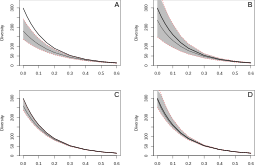
\includegraphics[width=1\linewidth]{images/Estimation} 

}

\caption{Estimation de la diversité d'une communauté log-normale de 300 espèces. Un inventaire de 500 (en bas) ou 5000 (en haut) individus est répété 1000 fois et la diversité estimée à chaque fois par l'estimateur de Chao-Wang-Jost (à gauche) ou l'estimateur révélé (à droite). La courbe noire en gras représente la vraie diversité de la communauté. La courbe maigre est la moyenne de l'estimation, l'enveloppe grise limitée par les pointillés rouges contient 95\% des valeurs simulées. A: 5000 individus, estimateur de Chao-Wang-Jost. B: 5000 individus, estimateur révélé. C: 500 individus, estimateur de Chao-Wang-Jost. D: 500 individus, estimateur révélé.}\label{fig:Estimation}
\end{SCfigure}

\normalsize

La figure \ref{fig:Estimation} compare les résultats des deux meilleurs estimateurs à la vraie valeur de la diversité d'une communauté de 300 espèces, dont la distribution log-normale (avec un écart-type dont le logarithme vaut 2) mime une forêt tropicale similaire à Barro-Colorado.
L'effort d'inventaire simulé est de 500 ou 5000 individus (de l'ordre d'un ou dix hectares pour les arbres de diamètre supérieur ou égal à 10~cm).
L'estimation ne pose pas de problème avec 5000 individus, bien que Chao-Wang-Jost sous-estime un peu le nombre d'espèces.
L'estimateur révélé est centré sur la vraie valeur, mais avec une plus grande variabilité.

En limitant l'échantillonnage à 500 individus, l'estimateur de Chao-Wang-Jost sous-estime le nombre d'espèces de moitié.
L'estimateur révélé sous-estime beaucoup moins la diversité d'ordre faible, mais son intervalle de confiance est très large.

Dès \(q=0,5\), l'estimation est très précise dans tous les cas, même en réduisant l'échantillonnage à 200 individus ou pour des communautés dont la queue de distribution est beaucoup plus longue (résultats non présentés ici).

Les conclusions de ce travail d'évaluation tiennent en deux points.
Dans des conditions réalistes d'inventaire d'arbres en forêt tropicale, les estimateurs de diversité les plus performants sont celui de Chao, Wang et Jost et l'estimateur révélé.
Le premier a une variance plus faible pour les valeurs de \(q\) proches de 0 mais est limité par son estimation du nombre d'espèces par l'estimateur Chao1.
Le second est préférable quand le nombre d'espèces estimé par l'estimateur jackknife d'ordre optimal est clairement supérieur (c'est-à-dire, en pratique, quand l'ordre du jacknife optimal est supérieur à 1).
Son biais est alors bien inférieur, au prix d'une variance plus grande.

Dans tous les cas, l'estimation de la diversité aux ordres inférieurs à 0,5 est imprécise, sauf à disposer d'inventaires de taille considérable (de l'ordre de la dizaine d'hectares au moins).

Les fonctions \texttt{Tsallis} et \texttt{Diversity}de \emph{entropart} acceptent comme argument un vecteur d'abondances (et non de probabilités) et proposent par défaut la correction de Chao et Jost:

\scriptsize

\begin{Shaded}
\begin{Highlighting}[]
\KeywordTok{Tsallis}\NormalTok{(}\KeywordTok{colSums}\NormalTok{(BCI), }\DataTypeTok{q =} \DecValTok{1}\NormalTok{)}
\end{Highlighting}
\end{Shaded}

\begin{verbatim}
##  UnveilJ 
## 4.276075
\end{verbatim}

\begin{Shaded}
\begin{Highlighting}[]
\KeywordTok{Diversity}\NormalTok{(}\KeywordTok{colSums}\NormalTok{(BCI), }\DataTypeTok{q =} \DecValTok{1}\NormalTok{)}
\end{Highlighting}
\end{Shaded}

\begin{verbatim}
##  UnveilJ 
## 71.95748
\end{verbatim}

\normalsize

\hypertarget{msom-et-msam}{%
\subsection{MSOM et MSAM}\label{msom-et-msam}}

L'utilisation de modèles hiérarchiques bayesiens fondés sur des modèles d'occupation multispécifiques (MSOM) ou des modèles d'abondance multispécifiques (MSAM) progresse dans la littérature récente.
Ils nécessitent de choisir une loi de probabilité d'observation des espèces compatible avec un échantillonnage non exhaustif, par exemple une loi ZIP (\emph{zero-inflated Poisson}) \autocite{Zhang2014c}, dans laquelle l'espérance de la présence de chaque espèce peut être modélisée à son tour comme la conséquence de variables environnementales.
Une approche alternative consiste à modéliser la probabilité d'observation comme la combinaison d'une probabilité de présence et d'une probabilité de détection \autocite{Broms2014}.
Ces méthodes ont l'avantage de fournir une distribution de probabilité des paramètres des modèles, et donc de la diversité qui est calculée comme une quantité dérivée. Leur faiblesse est qu'ils dépendent de la loi choisie. Une revue complète est fournie par \textcite{Iknayan2014}

\hypertarget{sec:RarExtrapol}{%
\subsection{Raréfaction et extrapolation}\label{sec:RarExtrapol}}

\textcite{Chao2014} étendent l'approche de \textcite{Gotelli2001} aux nombres de Hill et fournissent les méthodes nécessaires au calcul de courbes de raréfaction et d'extrapolation de l'estimateur de \(^{q}\!D\) en fonction de la taille de l'échantillon ou du taux de couverture.

Les courbes de raréfaction sont obtenues à partir de l'échantillon disponible en simulant la diminution de sa taille.
Les courbes d'extrapolation simulent l'augmentation de la taille de l'échantillon.
Elles sont en réalité calculées par raréfaction d'un échantillon hypothétique de taille infinie: un estimateur de \(^{q}\!D\) corrigé du biais d'estimation est nécessaire.
L'article se limite aux valeurs de \(q\) égales à 0, 1 ou 2 ou non entières mais supérieures à 2.
Le package \emph{iNEXT} \autocite{Hsieh2014} implémente ces calculs dans R comme le package \emph{entropart} qui améliore l'estimation des ordres non entiers de diversité.

\hypertarget{autres-approches}{%
\section{Autres approches}\label{autres-approches}}

\hypertarget{lentropie-de-ruxe9nyi}{%
\subsection{L'entropie de Rényi}\label{lentropie-de-ruxe9nyi}}

L'entropie d'ordre \(q\) de \textcite{Renyi1961} est

\begin{equation}
  \label{eq:Renyi}
  ^{q}\!R =\frac{1}{1-q\ln\sum^S_{q=1}{p^q_s}}.
\end{equation}

C'est le logarithme naturel des nombres de \textcite{Hill1973} qui ont été définis à partir d'elle.
L'entropie de Rényi a connu un succès important en tant que seule mesure d'entropie généralisée jusqu'à la diffusion de l'entropie HCDT.
Son défaut est qu'elle n'est pas forcément concave \autocite{Beck2009}, ce qui empêche sa décomposition (voir chapitre \ref{chap:DedompHCDT}).

\hypertarget{lentropie-guxe9nuxe9ralisuxe9e-des-mesures-dinuxe9galituxe9}{%
\subsection{L'entropie généralisée des mesures d'inégalité}\label{lentropie-guxe9nuxe9ralisuxe9e-des-mesures-dinuxe9galituxe9}}

L'entropie généralisée des économistes, d'ordre \(q\), est définie comme

\begin{equation}
  \label{eq:HqEco}
  H_q = \frac{1}{q\left(q-1\right)} \left[\frac{1}{S}\sum^S_{s=1}{\left(\frac{n_s}{\bar{n_s}}\right)^{q}}-1\right].
\end{equation}

C'est en réalité une entropie relative, qui mesure l'écart entre la distribution observée \(\{n_s\}\) et sa valeur moyenne. Elle tend vers l'entropie de Theil quand \(q \to 1\) et la moyenne des \(\ln(\frac{n_s}{\bar{n_s}})\) quand \(q \to 0\).
Elle a été conçue pour mesurer les inégalités \autocite{Cowell2000}, puis utilisée par exemple pour mesurer la concentration spatiale \autocite{Brulhart2005}.

\textcite{Maasoumi1993} explicite cet usage et pour comparer la distribution de probabilité observée \(\{q_s\}\) à une distribution attendue \(\{p_s\}\), plutôt qu'à la distribution uniforme dont toutes les valeurs seraient \(\frac{1}{S}\). En posant \(r=q-1\), en transformant les abondances \(\{n_s\}\) en probabilités \(\{q_s\}\) et en choisissant \(\{p_s\}\) arbitrairement, on obtient

\begin{equation}
  \label{eq:Maasoumi1993}
  H_r\left(\mathbf{q},\mathbf{p}\right) = \frac{1}{r\left(r+1\right)}\left[\sum^S_{s=1}{q_s{\left(\frac{q_s}{p_s}\right)}^{r}}-1\right].
\end{equation}

\textcite{Cressie1984} ont défini une mesure généralisée de qualité d'ajustement (\emph{Goodness of Fit}) de la distribution \(\{q_s\}\) à celle de \(\{p_s\}\).
Elle est identique à l'entropie généralisée (à un coefficient 2 près) bien que développée indépendamment pour d'autres motivations.
La statistique de Cressie et Read d'ordre 1 est la divergence de \textcite{Kullback1951}, celle d'ordre 2 le \(\chi^2\) de \textcite{Pearson1900}.

\textcite{Studeny2011} définissent une mesure d'équitabilité comme la divergence entre la distribution observée \(\{p_s\}\) et la distribution uniforme, ce qui les ramène à l'entropie de Cowell:

\begin{equation}
  \label{eq:Studeny2011}
  I_r 
  = \frac{1}{r\left(r+1\right)} \left[\sum^S_{s=1}{p_s \left(\frac{p_s}{1/S} \right)^{r}-1 } \right].
\end{equation}

Cette mesure inclut à la fois l'équitabilité et la richesse de la distribution.
Il s'agit donc d'une mesure de diversité, qui est, à une normalisation près, l'écart entre la valeur de l'entropie HCDT d'ordre \(q=r+1\) et sa valeur maximale.
Elle généralise donc l'indice de \textcite{Theil1967}:

\begin{equation}
  \label{eq:TheilGen}
  I_r = \frac{1}{q S^{1-q}}\left( \ln_q{S} - ^{q}\!H \right).
\end{equation}

\hypertarget{sec:SimpsonG}{%
\subsection{L'entropie de Simpson généralisée}\label{sec:SimpsonG}}

L'entropie de Simpson généralisée a été introduite dans une classe d'indices plus générale \eqref{eq:zeta} par \textcite{Zhang2010} et étudiée en détail par \textcite{Zhang2014}.
L'entropie d'ordre \(r>0\) est
\begin{equation}
  \label{eq:zetar}
  \zeta_r = \sum_{s=1}^S p_s (1-p_s)^r.
\end{equation}

Elle se réduit à l'entropie de Simpson pour \(r=1\).

La fonction d'information de l'entropie de Simpson généralisée \(I(p)=(1-p)^r\) représente la probabilité de n'observer aucun individu de l'espèce de probabilité \(p\) dans un échantillon de taille \(r\): c'est une mesure intuitive de la rareté.
\textcite{Chao2013} ont interprété \(\zeta_r\) comme la probabilité qu'un individu échantillonné au rang \(r+1\) appartienne à une espèce nouvelle dans une SAC.
\((r+1)\zeta_r\) est aussi l'espérance du nombre de singletons dans un échantillon de taille \((r+1)\).

L'intérêt majeur de cette entropie est qu'elle dispose d'un estimateur non biaisé pour toutes les valeurs de \(r\) strictement inférieures à la taille de l'échantillon.
C'est une mesure de diversité valide pour les ordres \(r\) strictement inférieurs au nombre d'espèces \autocite{Grabchak2016}.
Au-delà, elle ne respecte plus l'axiome d'équitabilité: sa valeur maximale n'est pas obtenue quand les espèces sont équiprobables.

Son nombre effectif d'espèces est
\begin{equation}
  \label{eq:Dzeta}
  ^{r}\!D^{\zeta} = \frac{1}{1 - \zeta_r^{\frac{1}{r}}}.
\end{equation}

L'existence d'un estimateur sans biais et d'un intervalle de confiance calculable analytiquement permet de comparer des profils de diversité de façon robuste quand l'échantillonnage est limité et la richesse élevée.

La figure \ref{fig:comProfilzetaFig}a montre les profils de diversité (en nombre effectifs d'espèces) des deux parcelles 6 et 18 de Paracou: 1~ha inventorié, respectivement 681 et 483 arbres, pour une richesse estimée à 254 et 309 espèces par les estimateurs jackknife d'ordres 2 et 3:

\scriptsize

\begin{Shaded}
\begin{Highlighting}[]
\NormalTok{NsP6 <-}\StringTok{ }\KeywordTok{as.AbdVector}\NormalTok{(Paracou618.MC}\OperatorTok{$}\NormalTok{Nsi[, }\DecValTok{1}\NormalTok{])}
\NormalTok{(S6 <-}\StringTok{ }\KeywordTok{Richness}\NormalTok{(NsP6, }\DataTypeTok{Correction =} \StringTok{"Jackknife"}\NormalTok{))}
\end{Highlighting}
\end{Shaded}

\begin{verbatim}
## Jackknife 2 
##         254
\end{verbatim}

\begin{Shaded}
\begin{Highlighting}[]
\NormalTok{NsP18 <-}\StringTok{ }\KeywordTok{as.AbdVector}\NormalTok{(Paracou618.MC}\OperatorTok{$}\NormalTok{Nsi[, }\DecValTok{2}\NormalTok{])}
\NormalTok{(S18 <-}\StringTok{ }\KeywordTok{Richness}\NormalTok{(NsP18, }\DataTypeTok{Correction =} \StringTok{"Jackknife"}\NormalTok{))}
\end{Highlighting}
\end{Shaded}

\begin{verbatim}
## Jackknife 3 
##         309
\end{verbatim}

\begin{Shaded}
\begin{Highlighting}[]
\NormalTok{S <-}\StringTok{ }\KeywordTok{min}\NormalTok{(S6, S18)}
\end{Highlighting}
\end{Shaded}

\normalsize

En comparaison, la figure \ref{fig:comProfilzetaFig}b montre les profils de diversité HCDT des mêmes parcelles.
Ils se chevauchent pour les petits ordres de diversité, ce qui ne permet pas de conclure.



\scriptsize

\begin{SCfigure}

{\centering 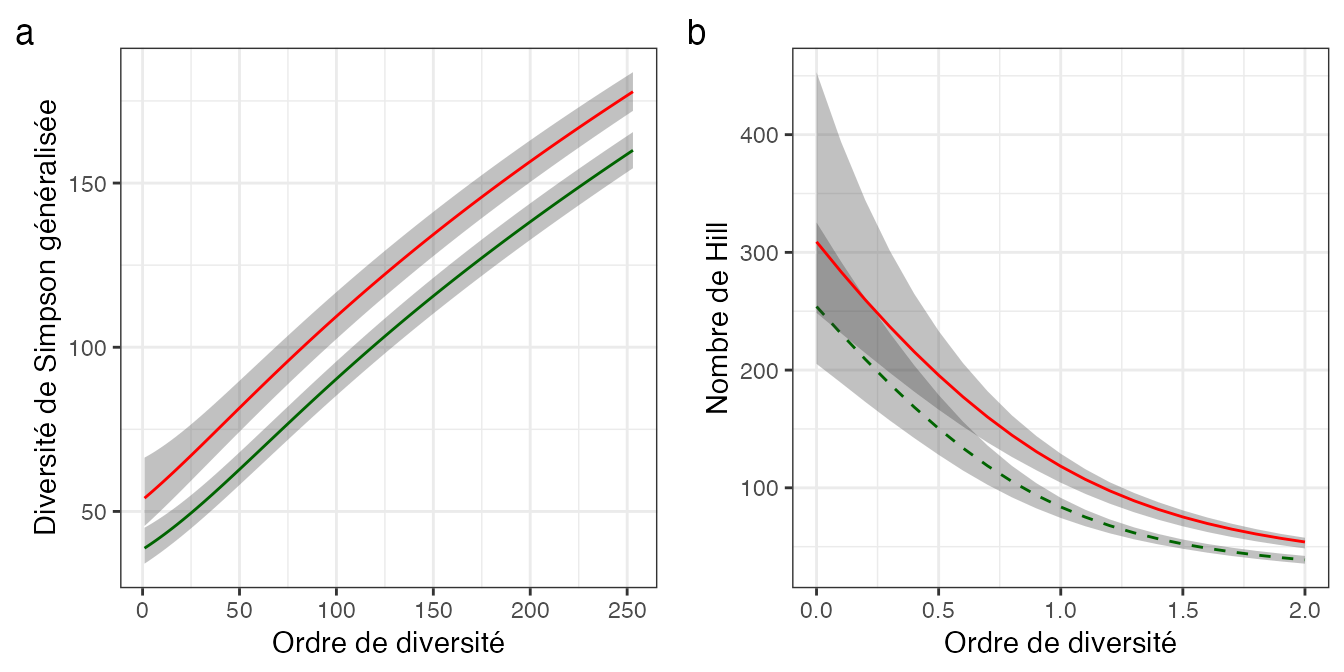
\includegraphics[width=1\linewidth]{MesuresBD_files/figure-latex/comProfilzetaFig-1} 

}

\caption{Comparaison des profils de diversité des parcelles 6 et 18 de Paracou avec leur intervalle de confiance à 95\%. La parcelle 18 est tracée en rouge, lignes continues, et la 6 en vert, lignes pointillées. (a) Diversité généralisée de Simpson (nombres effectif d'espèces): les profils sont distincts, ce qui permet de conclure que la parcelle 6 est plus diverse que la parcelle 18. (b) Diversité HCDT: les profils se chevauchent jusqu'à \(q \approx 0,7\).}\label{fig:comProfilzetaFig}
\end{SCfigure}

\normalsize

La diversité est donc estimée jusqu'à l'ordre 253.

Code R pour réaliser la figure \ref{fig:comProfilzetaFig}:

\scriptsize

\begin{Shaded}
\begin{Highlighting}[]
\CommentTok{# Profil P6}
\KeywordTok{library}\NormalTok{(}\StringTok{"EntropyEstimation"}\NormalTok{)}
\NormalTok{zeta6 <-}\StringTok{ }\KeywordTok{CommunityProfile}\NormalTok{(GenSimpson, NsP6, }\DecValTok{1}\OperatorTok{:}\NormalTok{(S }\OperatorTok{-}\StringTok{ }\DecValTok{1}\NormalTok{))}
\NormalTok{sigma6 <-}\StringTok{ }\KeywordTok{sapply}\NormalTok{(}\DecValTok{1}\OperatorTok{:}\NormalTok{(S }\OperatorTok{-}\StringTok{ }\DecValTok{1}\NormalTok{), }\ControlFlowTok{function}\NormalTok{(r) }\KeywordTok{GenSimp.sd}\NormalTok{(NsP6, r))}
\NormalTok{ic6 <-}\StringTok{ }\KeywordTok{qnorm}\NormalTok{(}\DecValTok{1} \OperatorTok{-}\StringTok{ }\FloatTok{0.05}\OperatorTok{/}\DecValTok{2}\NormalTok{) }\OperatorTok{*}\StringTok{ }\NormalTok{sigma6}\OperatorTok{/}\KeywordTok{sqrt}\NormalTok{(}\KeywordTok{sum}\NormalTok{(NsP6))}
\NormalTok{zeta6}\OperatorTok{$}\NormalTok{low <-}\StringTok{ }\NormalTok{zeta6}\OperatorTok{$}\NormalTok{y }\OperatorTok{-}\StringTok{ }\NormalTok{ic6}
\NormalTok{zeta6}\OperatorTok{$}\NormalTok{high <-}\StringTok{ }\NormalTok{zeta6}\OperatorTok{$}\NormalTok{y }\OperatorTok{+}\StringTok{ }\NormalTok{ic6}
\CommentTok{# Profil P18}
\NormalTok{zeta18 <-}\StringTok{ }\KeywordTok{CommunityProfile}\NormalTok{(GenSimpson, NsP18, }\DecValTok{1}\OperatorTok{:}\NormalTok{(S }\OperatorTok{-}\StringTok{ }\DecValTok{1}\NormalTok{))}
\NormalTok{sigma18 <-}\StringTok{ }\KeywordTok{sapply}\NormalTok{(}\DecValTok{1}\OperatorTok{:}\NormalTok{(S }\OperatorTok{-}\StringTok{ }\DecValTok{1}\NormalTok{), }\ControlFlowTok{function}\NormalTok{(r) }\KeywordTok{GenSimp.sd}\NormalTok{(NsP18, r))}
\NormalTok{ic18 <-}\StringTok{ }\KeywordTok{qnorm}\NormalTok{(}\DecValTok{1} \OperatorTok{-}\StringTok{ }\FloatTok{0.05}\OperatorTok{/}\DecValTok{2}\NormalTok{) }\OperatorTok{*}\StringTok{ }\NormalTok{sigma18}\OperatorTok{/}\KeywordTok{sqrt}\NormalTok{(}\KeywordTok{sum}\NormalTok{(NsP18))}
\NormalTok{zeta18}\OperatorTok{$}\NormalTok{low <-}\StringTok{ }\NormalTok{zeta18}\OperatorTok{$}\NormalTok{y }\OperatorTok{-}\StringTok{ }\NormalTok{ic18}
\NormalTok{zeta18}\OperatorTok{$}\NormalTok{high <-}\StringTok{ }\NormalTok{zeta18}\OperatorTok{$}\NormalTok{y }\OperatorTok{+}\StringTok{ }\NormalTok{ic18}
\CommentTok{# Transformation en diversité}
\NormalTok{zeta6D <-}\StringTok{ }\NormalTok{zeta6}
\NormalTok{zeta6D}\OperatorTok{$}\NormalTok{y <-}\StringTok{ }\DecValTok{1}\OperatorTok{/}\NormalTok{(}\DecValTok{1} \OperatorTok{-}\StringTok{ }\NormalTok{(zeta6}\OperatorTok{$}\NormalTok{y)}\OperatorTok{^}\NormalTok{(}\DecValTok{1}\OperatorTok{/}\NormalTok{zeta6}\OperatorTok{$}\NormalTok{x))}
\NormalTok{zeta6D}\OperatorTok{$}\NormalTok{low <-}\StringTok{ }\DecValTok{1}\OperatorTok{/}\NormalTok{(}\DecValTok{1} \OperatorTok{-}\StringTok{ }\NormalTok{(zeta6}\OperatorTok{$}\NormalTok{low)}\OperatorTok{^}\NormalTok{(}\DecValTok{1}\OperatorTok{/}\NormalTok{zeta6}\OperatorTok{$}\NormalTok{x))}
\NormalTok{zeta6D}\OperatorTok{$}\NormalTok{high <-}\StringTok{ }\DecValTok{1}\OperatorTok{/}\NormalTok{(}\DecValTok{1} \OperatorTok{-}\StringTok{ }\NormalTok{(zeta6}\OperatorTok{$}\NormalTok{high)}\OperatorTok{^}\NormalTok{(}\DecValTok{1}\OperatorTok{/}\NormalTok{zeta6}\OperatorTok{$}\NormalTok{x))}
\NormalTok{zeta18D <-}\StringTok{ }\NormalTok{zeta18}
\NormalTok{zeta18D}\OperatorTok{$}\NormalTok{y <-}\StringTok{ }\DecValTok{1}\OperatorTok{/}\NormalTok{(}\DecValTok{1} \OperatorTok{-}\StringTok{ }\NormalTok{(zeta18}\OperatorTok{$}\NormalTok{y)}\OperatorTok{^}\NormalTok{(}\DecValTok{1}\OperatorTok{/}\NormalTok{zeta18}\OperatorTok{$}\NormalTok{x))}
\NormalTok{zeta18D}\OperatorTok{$}\NormalTok{low <-}\StringTok{ }\DecValTok{1}\OperatorTok{/}\NormalTok{(}\DecValTok{1} \OperatorTok{-}\StringTok{ }\NormalTok{(zeta18}\OperatorTok{$}\NormalTok{low)}\OperatorTok{^}\NormalTok{(}\DecValTok{1}\OperatorTok{/}\NormalTok{zeta18}\OperatorTok{$}\NormalTok{x))}
\NormalTok{zeta18D}\OperatorTok{$}\NormalTok{high <-}\StringTok{ }\DecValTok{1}\OperatorTok{/}\NormalTok{(}\DecValTok{1} \OperatorTok{-}\StringTok{ }\NormalTok{(zeta18}\OperatorTok{$}\NormalTok{high)}\OperatorTok{^}\NormalTok{(}\DecValTok{1}\OperatorTok{/}\NormalTok{zeta18}\OperatorTok{$}\NormalTok{x))}
\CommentTok{# Figure}
\NormalTok{gga <-}\StringTok{ }\KeywordTok{ggplot}\NormalTok{() }\OperatorTok{+}\StringTok{ }
\StringTok{  }\KeywordTok{geom_ribbon}\NormalTok{(}\KeywordTok{aes}\NormalTok{(x, }\DataTypeTok{ymin =}\NormalTok{ low, }\DataTypeTok{ymax =}\NormalTok{ high), }
              \KeywordTok{as.data.frame.list}\NormalTok{(zeta18D), }\DataTypeTok{alpha =} \FloatTok{0.3}\NormalTok{) }\OperatorTok{+}
\StringTok{  }\KeywordTok{geom_line}\NormalTok{(}\KeywordTok{aes}\NormalTok{(x, y), }\KeywordTok{as.data.frame.list}\NormalTok{(zeta18D), }\DataTypeTok{col =} \StringTok{"red"}\NormalTok{) }\OperatorTok{+}
\StringTok{  }\KeywordTok{geom_ribbon}\NormalTok{(}\KeywordTok{aes}\NormalTok{(x, }\DataTypeTok{ymin =}\NormalTok{ low, }\DataTypeTok{ymax =}\NormalTok{ high), }
              \KeywordTok{as.data.frame.list}\NormalTok{(zeta6D), }\DataTypeTok{alpha =} \FloatTok{0.3}\NormalTok{) }\OperatorTok{+}
\StringTok{  }\KeywordTok{geom_line}\NormalTok{(}\KeywordTok{aes}\NormalTok{(x, y), }\KeywordTok{as.data.frame.list}\NormalTok{(zeta6D), }\DataTypeTok{col =} \StringTok{"darkgreen"}\NormalTok{) }\OperatorTok{+}
\StringTok{  }\KeywordTok{labs}\NormalTok{(}\DataTypeTok{x =} \StringTok{"Ordre de diversité"}\NormalTok{, }
       \DataTypeTok{y =} \StringTok{"Diversité de Simpson généralisée"}\NormalTok{) }\OperatorTok{+}
\StringTok{  }\KeywordTok{labs}\NormalTok{(}\DataTypeTok{tag =} \StringTok{"a"}\NormalTok{)}
\CommentTok{# Calcul des profils HCDT}
\NormalTok{D6 <-}\StringTok{ }\KeywordTok{CommunityProfile}\NormalTok{(Diversity, NsP6, }\DataTypeTok{NumberOfSimulations =} \DecValTok{10}\NormalTok{,}
\DataTypeTok{q.seq=}\NormalTok{q.seq, }\DataTypeTok{Correction =} \StringTok{"UnveilJ"}\NormalTok{)}
\NormalTok{D18 <-}\StringTok{ }\KeywordTok{CommunityProfile}\NormalTok{(Diversity, NsP18, }\DataTypeTok{NumberOfSimulations =} \DecValTok{10}\NormalTok{,}
\DataTypeTok{q.seq=}\NormalTok{q.seq, }\DataTypeTok{Correction =} \StringTok{"UnveilJ"}\NormalTok{)}
\CommentTok{# Figure}
\NormalTok{ggb <-}\StringTok{ }\KeywordTok{ggplot}\NormalTok{(}\KeywordTok{data.frame}\NormalTok{(}\DataTypeTok{x =}\NormalTok{ D6}\OperatorTok{$}\NormalTok{x, D6}\OperatorTok{$}\NormalTok{y, D18}\OperatorTok{$}\NormalTok{y)) }\OperatorTok{+}
\StringTok{  }\KeywordTok{geom_ribbon}\NormalTok{(}\KeywordTok{aes}\NormalTok{(x, }\DataTypeTok{ymin =}\NormalTok{ low, }\DataTypeTok{ymax =}\NormalTok{ high), }\KeywordTok{as.data.frame.list}\NormalTok{(D6), }
              \DataTypeTok{alpha =} \FloatTok{0.3}\NormalTok{) }\OperatorTok{+}
\StringTok{  }\KeywordTok{geom_line}\NormalTok{(}\KeywordTok{aes}\NormalTok{(x, D6.y), }\DataTypeTok{col =} \StringTok{"darkgreen"}\NormalTok{, }\DataTypeTok{lty =} \DecValTok{2}\NormalTok{) }\OperatorTok{+}\StringTok{ }
\StringTok{  }\KeywordTok{geom_ribbon}\NormalTok{(}\KeywordTok{aes}\NormalTok{(x, }\DataTypeTok{ymin =}\NormalTok{ low, }\DataTypeTok{ymax =}\NormalTok{ high), }\KeywordTok{as.data.frame.list}\NormalTok{(D18), }
              \DataTypeTok{alpha =} \FloatTok{0.3}\NormalTok{) }\OperatorTok{+}
\StringTok{  }\KeywordTok{geom_line}\NormalTok{(}\KeywordTok{aes}\NormalTok{(x, D18.y), }\DataTypeTok{col =} \StringTok{"red"}\NormalTok{) }\OperatorTok{+}\StringTok{ }
\StringTok{  }\KeywordTok{labs}\NormalTok{(}\DataTypeTok{x =} \StringTok{"Ordre de diversité"}\NormalTok{, }\DataTypeTok{y =} \StringTok{"Nombre de Hill"}\NormalTok{) }\OperatorTok{+}
\StringTok{  }\KeywordTok{labs}\NormalTok{(}\DataTypeTok{tag =} \StringTok{"b"}\NormalTok{)}
\KeywordTok{grid.arrange}\NormalTok{(gga, ggb, }\DataTypeTok{ncol =} \DecValTok{2}\NormalTok{)}
\end{Highlighting}
\end{Shaded}

\normalsize

La distribution statistique de la différence d'entropie est connue, et peut donc être tracée (figure \ref{fig:zetaDiffFig}).
Son intervalle de confiance ne contient jamais la valeur 0, ce qui permet de conclure que la parcelle 18 est plus diverse.



\scriptsize

\begin{SCfigure}

{\centering 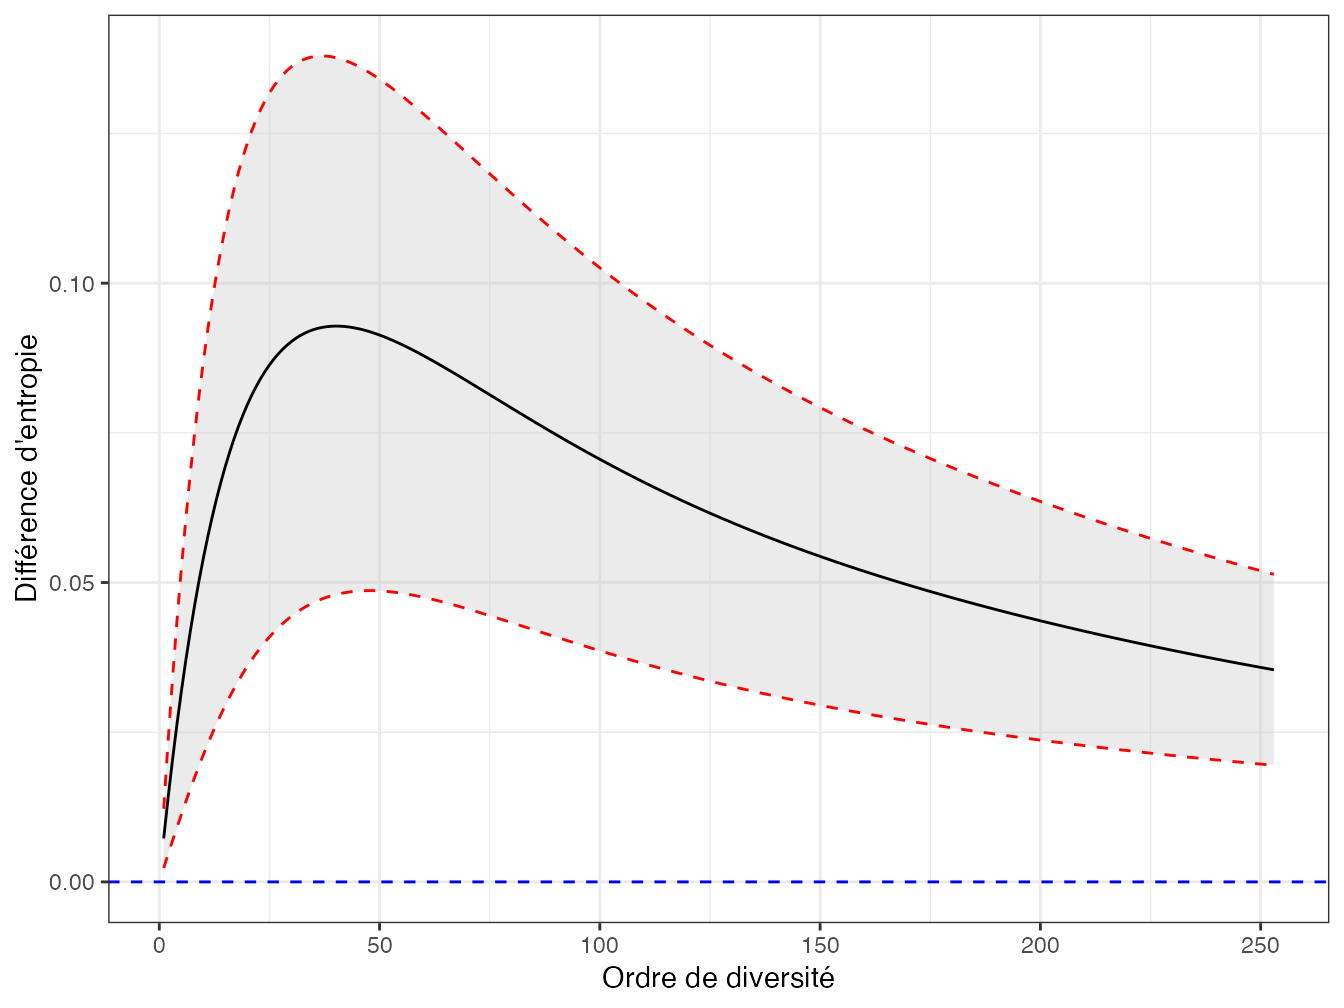
\includegraphics[width=0.8\linewidth]{MesuresBD_files/figure-latex/zetaDiffFig-1} 

}

\caption{Différence entre les entropies de Simpson généralisées des parcelles 18 et 6 de Paracou avec son intervalle de confiance à 95\%. La ligne horizontale représente l'hypothèse nulle d'égalité entre les entropies, qui peut être rejetée.}\label{fig:zetaDiffFig}
\end{SCfigure}

\normalsize

Code R pour réaliser la figure:

\scriptsize

\begin{Shaded}
\begin{Highlighting}[]
\CommentTok{# Calcul de P18-P6 avec IC}
\NormalTok{  Difference <-}\StringTok{ }\KeywordTok{list}\NormalTok{(}\DataTypeTok{x =}\NormalTok{ zeta18}\OperatorTok{$}\NormalTok{x, }\DataTypeTok{y =}\NormalTok{ zeta18}\OperatorTok{$}\NormalTok{y}\OperatorTok{-}\NormalTok{zeta6}\OperatorTok{$}\NormalTok{y)}
  \KeywordTok{class}\NormalTok{(Difference) <-}\StringTok{ }\KeywordTok{class}\NormalTok{(zeta18)}
\NormalTok{  icDifference <-}\StringTok{ }\KeywordTok{qnorm}\NormalTok{(}\DecValTok{1}\FloatTok{-0.05}\OperatorTok{/}\DecValTok{2}\NormalTok{)}\OperatorTok{*}\KeywordTok{sqrt}\NormalTok{(sigma6}\OperatorTok{^}\DecValTok{2}\OperatorTok{/}\KeywordTok{sum}\NormalTok{(NsP6) }
                                       \OperatorTok{+}\StringTok{ }\NormalTok{sigma18}\OperatorTok{^}\DecValTok{2}\OperatorTok{/}\KeywordTok{sum}\NormalTok{(NsP18))}
\NormalTok{  Difference}\OperatorTok{$}\NormalTok{low <-}\StringTok{ }\NormalTok{Difference}\OperatorTok{$}\NormalTok{y }\OperatorTok{-}\StringTok{ }\NormalTok{icDifference}
\NormalTok{  Difference}\OperatorTok{$}\NormalTok{high <-}\StringTok{ }\NormalTok{Difference}\OperatorTok{$}\NormalTok{y }\OperatorTok{+}\StringTok{ }\NormalTok{icDifference}
  \CommentTok{# Plot}
  \KeywordTok{autoplot}\NormalTok{(Difference, }\DataTypeTok{xlab =} \StringTok{"Ordre de diversité"}\NormalTok{, }
           \DataTypeTok{ylab =} \StringTok{"Différence d'entropie"}\NormalTok{) }\OperatorTok{+}\StringTok{ }
\StringTok{    }\KeywordTok{geom_hline}\NormalTok{(}\DataTypeTok{yintercept =} \DecValTok{0}\NormalTok{, }\DataTypeTok{col =} \StringTok{"blue"}\NormalTok{, }\DataTypeTok{lty =} \DecValTok{2}\NormalTok{)}
\end{Highlighting}
\end{Shaded}

\normalsize

La prise en compte des espèces rares est limitée par la valeur maximale de l'ordre \(r\) (limité à \(S-1\)).
Les espèces plus rares ne peuvent pas être prises en compte: le profil de diversité s'arrête là.
Le nombre effectif d'espèces maximum correspond au nombre de Hill d'ordre 0,5 environ.
Les espèces plus rares sont prises en compte dans la partie du profil de diversité HCDT d'ordre inférieur à 0,5 mais son incertitude est grande et son biais très important quand l'échantillonnage est aussi réduit \autocite{Marcon2015a}.

L'entropie de Simpson généralisée est donc l'outil le plus approprié pour comparer des profils de diversité de communautés riches et sous-échantillonnées.

\hypertarget{lentropie-par-cas}{%
\subsection{L'entropie par cas}\label{lentropie-par-cas}}

\textcite{Rajaram2016} décomposent la diversité de Shannon en produit des contributions de chaque catégorie et proposent une mesure cumulative de la diversité d'une communauté prenant en compte une partie des espèces classées selon un critère pertinent, décrivant leur complexité: par exemple, la diversité des mammifères classés par taille croissante, ou la position dans l'évolution.

La fraction de la communauté dont le cumul des probabilités égale \(c\) est prise en compte.
La diversité cumulée est:
\begin{equation}
  \label{eq:Rajaram2016Dc}
  \mathit{D_c} = \prod_c{p_s^{-p_s}}.
\end{equation}

La mesure normalisée est appelée \emph{case-based entropy} en anglais et vaut
\begin{equation}
  \label{eq:Rajaram2016Cc}
  \mathit{C_c} = \frac{100 D_c}{^{1}\!D}.
\end{equation}

\(\mathit{D_c}={^{1}\!D}\) quand toute la communauté est prise en compte (\(c=1\)).
Les auteurs s'intéressent principalement à la courbe de \(C_c\) en fonction de \(c\) pour montrer \autocite{Castellani2016} que la contribution à la diversité totale des 40\% des composants les moints complexes de systèmes très divers (``des galaxies au gènes'') atteint toujours au moins 60\%, ce résultat étant interprété comme une loi universelle de limitation de la complexité.

Cette mesure peut être étendue à l'entropie HCDT sans difficulté:
\begin{equation}
  \label{eq:Ccq}
  \mathit{^{q}\!C_{c}} = {\left(\sum_c{p^q_s}\right)}^{\frac{1}{1-q}}.
\end{equation}

La méthode peut être appliquée pour évaluer la contribution de n'importe quel partie de la communauté à la diversité totale.
Il ne s'agit pas d'une décomposition de la diversité au sens classique du terme, qui consiste à partitionner la diversité totale en diversité intra et inter-groupes, mais plutôt d'une façon de prendre en compte les caractéristiques des espèces dans une approche non-neutre.

\hypertarget{sec:Equitabilite}{%
\chapter{Équitabilité}\label{sec:Equitabilite}}

\scriptsize

\begin{Essentiel}
L'équitabilité mesure l'écart entre la distribution observée et une
distribution uniforme.

L'indice de Pielou est la mesure d'équitabilité la plus connue. Il a été
généralisé pour permettre de pondérer plus ou moins les espèces rares,
de la même façon que l'entropie HCDT.
\end{Essentiel}

\normalsize

La régularité d'une distribution est une notion intuitivement assez simple: la faiblesse de l'écart entre la distribution réelle et une distribution parfaitement régulière \autocite{Lloyd1964}, vérifiant \(p_s={1}/{S}\).
Des difficultés apparaissent quand il s'agit de comparer l'équitabilité de communautés de richesses différentes.
L'approche axiomatique est présentée, puis les différents indices de la littérature et enfin la généralisation de l'indice de Pielou, en cohérence avec l'entropie HCDT.

\hypertarget{approche-axiomatique}{%
\section{Approche axiomatique}\label{approche-axiomatique}}

Une approche axiomatique a été développée par la littérature, revue par \textcite{Jost2010} ou \textcite{Tuomisto2012} Les propriétés fondamentales sont les critères de \textcite{Dalton1920}:

\begin{itemize}
\tightlist
\item
  L'équitabilité augmente quand un individu est transféré d'une espèce fréquente à une espèce rare;
\item
  L'équitabilité diminue quand une espèce rare est ajoutée;
\item
  Invariance d'échelle: l'équitabilité ne dépend que des fréquences, pas des abondances absolues.
\end{itemize}



\scriptsize

\begin{SCfigure}

{\centering 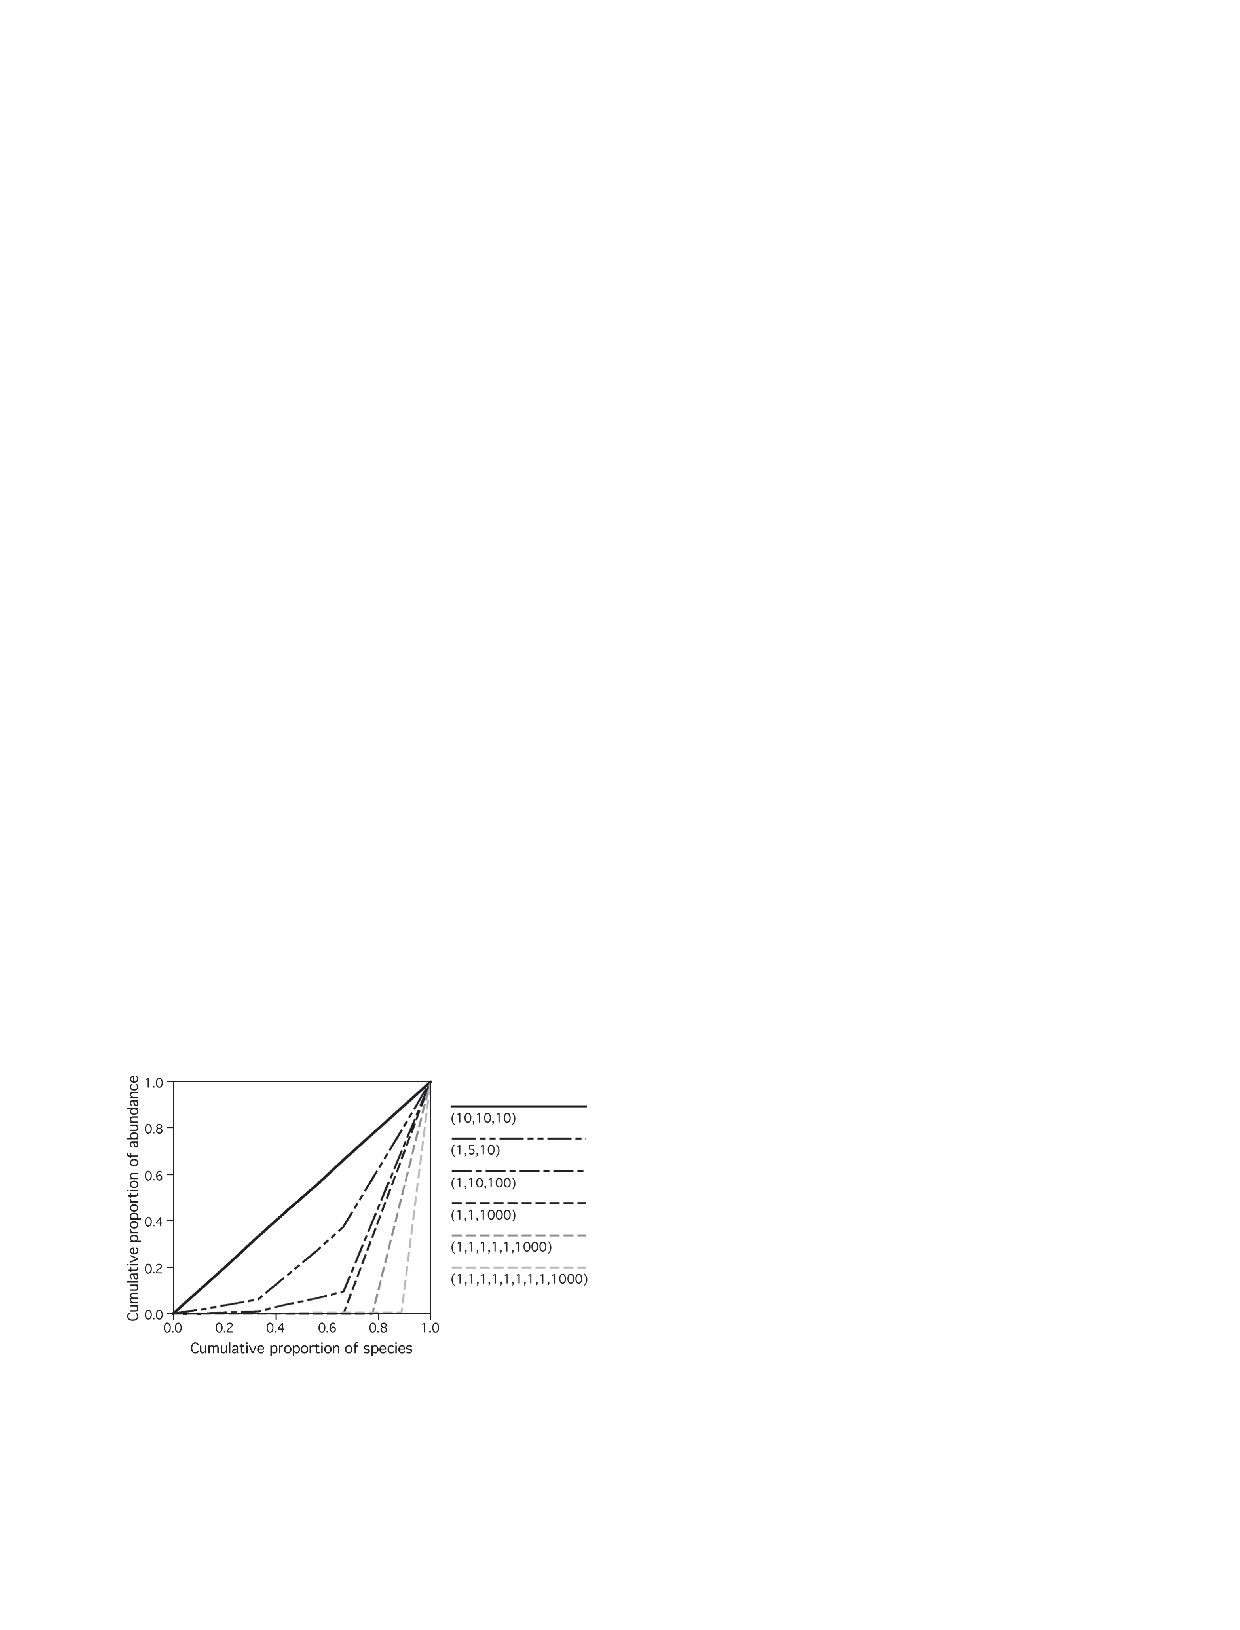
\includegraphics[width=0.8\linewidth]{images/Tuomisto2012} 

}

\caption{Tuomisto2012}\label{fig:Tuomisto2012}
\end{SCfigure}

\normalsize

Un critère supplémentaire établi par \textcite{Smith1996}, complété par \textcite{Gosselin2001} est la compatibilité avec la courbe de \textcite{Lorenz1905}, construite en classant les espèces de la moins fréquente à la plus fréquente, et en traçant le cumul des fréquences en fonction du rang \autocite[figure \ref{fig:Tuomisto2012},][]{Tuomisto2012}: une communauté parfaitement équitable est représentée par la bissectrice.
La surface entre la courbe réelle et la bissectrice est très utilisée en économie pour mesurer l'inégalité sous le nom d'``indice de Gini'' \autocite{Gini1912,Ceriani2012}:

\begin{itemize}
\tightlist
\item
  Compatibilité avec la courbe de Lorenz: l'équitabilité augmente pour une communauté si sa courbe de Lorenz est plus proche de la bissectrice.
  Si les courbes de deux communautés se croisent, l'ordre de leurs équitabilités est imprévisible.
\end{itemize}

Ce critère est remis en cause par \textcite{Ricotta2004}: il est incompatible \autocite{Routledge1983} avec le critère de continuité retenu pour les mesures de diversité: l'introduction d'une espèce supplémentaire avec une probabilité infinitésimale peut modifier considérablement l'équitabilité.

L'invariance par réplication est une propriété nécessaire (mais pas suffisante) à la compatibilité avec la courbe de Lorenz \autocite{Ricotta2004}:

\begin{itemize}
\tightlist
\item
  Invariance par réplication: l'équitabilité ne change pas si chaque espèce est remplacée par plusieurs nouvelles espèces ayant la même abondance.
\end{itemize}

Cette propriété est retenue par Tuomisto mais rejetée par Jost comme par Ricotta et d'autres.
L'argumentation de Jost est la plus convaincante: une communauté d'une richesse donnée dans laquelle tous les individus (à l'exception d'un nombre négligeable) sont concentrés dans une seule espèce atteint le niveau minimum d'équitabilité.
Si elle est dupliquée, les individus seront répartis dans deux espèces et non une: la nouvelle communauté n'atteindra pas le niveau minimum d'équitabilité, il est donc souhaitable que la mesure d'équitabilité augmente.

\hypertarget{indice-classiques}{%
\section{Indice classiques}\label{indice-classiques}}

\hypertarget{indice-de-bulla}{%
\subsection{Indice de Bulla}\label{indice-de-bulla}}

L'indice d'équitabilité de \textcite{Bulla1994} respecte les critères de Smith et Wilson:
\begin{equation}
  \label{eq:Bulla}
  O = \sum_s{\min(p_s,\frac{1}{S})}.
\end{equation}

Il mesure l'écart entre la distribution réelle et une distribution parfaitement équitable.
Bulla le normalise pour qu'il soit compris entre 0 et 1:
\begin{equation}
  \label{eq:BullaNorm}
  E_O = \frac{O - \min{O}}{1 - \min{O}}.
\end{equation}

La valeur minimale de \(O\) est \({1}/{S}\).
Bulla considère que ce n'est pas le cas si les effectifs sont entiers et fournit une valeur exacte dépendant du nombre d'espèces.

\hypertarget{indice-de-gini}{%
\subsection{Indice de Gini}\label{indice-de-gini}}

L'indice de Gini est le double de la surface comprise entre la courbe de Lorenz et la bissectrice (figure \ref{fig:Tuomisto2012}).

\hypertarget{rapports-de-moyennes}{%
\subsection{Rapports de moyennes}\label{rapports-de-moyennes}}

\textcite{Taillie1979} propose le rapport de la moyenne géométrique ou de la moyenne harmonique à la moyenne arithmétique des probabilités.

\hypertarget{ratios-de-hill}{%
\subsection{Ratios de Hill}\label{ratios-de-hill}}

\textcite{Hill1973} utilise les rapports entre nombres effectifs d'espèces d'ordres différents comme mesure d'équitabilité.
\(E_{1,0} = {^{1}\!D}/{^{0}\!D}\) avait déjà été proposé par \textcite{Sheldon1969}.
\textcite{Peet1974} le normalise en retirant au numérateur et au dénominateur leur valeur minimale, c'est-à-dire 1.

La version normalisée de \(E_{2,1}\) est recommandée par \textcite{Alatalo1981}.

\hypertarget{synthuxe8se-1}{%
\subsection{Synthèse}\label{synthuxe8se-1}}

\textcite{Ricotta2001} testent ces indices sur 65 jeux de données différents pour observer leurs corrélations.
Tous sont compatibles avec la courbe de Lorenz.
Ils concluent que les indices se répartissent en deux groupes: la plupart sont sensibles aux abondances relatives des espèces rares.
\(E_{\infty,0}\) et, dans une moindre mesure, \(E_{2,0}\) sont plus sensibles aux espèces fréquentes.

\hypertarget{indice-alternatifs}{%
\section{Indice alternatifs}\label{indice-alternatifs}}

\hypertarget{variance-de-la-raretuxe9}{%
\subsection{Variance de la rareté}\label{variance-de-la-raretuxe9}}

\textcite{Engen1977} définit comme mesure d'équitabilité la variance de la rareté (la fonction d'information) de l'entropie de Shannon (\(-\ln p\)):
\begin{equation}
  \label{eq:Engen1977}
  E_\mathit{VS} = \sum_{s}{p_s(\ln p_s)^2}-(\sum_s{p_s \ln p_s})^2.
\end{equation}

Sa valeur est nulle si les espèces sont équiprobables.

\textcite{Ricotta2003b} généralise cette mesure aux autres fonctions d'information.
Toutes peuvent être utilisées:

\begin{equation}
  \label{eq:Ricotta2003b}
  E_\mathit{VR} = \sum_{s}{p_s I(p_s)^2}-[\sum_s{p_s I(p_s)}]^2.
\end{equation}

Ces mesures ne sont pas invariantes par réplication mais sont continues par rapport aux probabilités.

\hypertarget{non-spuxe9cificituxe9}{%
\subsection{Non-spécificité}\label{non-spuxe9cificituxe9}}

\textcite{Ricotta2004} propose un indice fondé sur les ensembles flous, utilisant les mesures de spécificité \autocite{Yager1992}.
Les espèces sont classées par probabilité décroissante. La mesure de non-spécificité utilisable comme mesure d'équitabilité est

\begin{equation}
  \label{eq:Ricotta2004}
  E_\mathit{NSp} = \sum_{s=1}^{S-1}{\frac{p_s-p_{s+1}}{s}}.
\end{equation}

Cet indice n'est pas invariant par réplication mais est continu par rapport aux probabilités.

\hypertarget{indice-de-pielou}{%
\section{Indice de Pielou}\label{indice-de-pielou}}

Une expression de l'équitabilité est souvent donnée à partir de l'indice de Shannon \autocite{Lloyd1964,Sheldon1969,Pielou1966a,Pielou1975}.
La valeur maximale de l'indice de Shannon est obtenue quand la distribution est parfaitement régulière.
Alors: \(H_{\max}=\ln S\).
On a donc défini l'indice, souvent appelé ``indice de Pielou'':

\begin{equation}
  \label{eq:JPielou}
  J = \frac{H}{H_{\max}} = \frac{H}{\ln S}.
\end{equation}

\(J\) est compris entre 0 (une seule espèce a une probabilité de 1) et 1 (toutes les espèces ont la même probabilité).

\hypertarget{guxe9nuxe9ralisation-de-lindice-de-pielou}{%
\section{Généralisation de l'indice de Pielou}\label{guxe9nuxe9ralisation-de-lindice-de-pielou}}

\hypertarget{sec:Mendes}{%
\subsection{Mendes et al.~}\label{sec:Mendes}}

\textcite{Mendes2008} généralisent l'indice de Pielou en remplaçant l'indice de Shannon par l'entropie de Tsallis.
Ils définissent

\begin{equation}
  \label{eq:JMendes2008}
  ^{q}\!J^{*} = \frac{^{q}\!H}{^{q}H_{\max}} = \frac{^{q}\!H}{\ln_q{S}}
\end{equation}

et tracent des profils d'équitabilité, c'est-à-dire la valeur de \(^{q}\!J^{*}\) en fonction de \(q\).
Ils observent que l'équitabilité est minimale pour une valeur particulière de \(q\) qu'ils notent \(q^*\) et montrent sur des exemples simulés que \(q^*\) diminue avec la richesse de la communauté, mais sans en explorer complètement les propriétés.

\(^{2}\!J^{*}\) est l'indice d'équitabilité dérivé de l'indice de diversité de Simpson par \textcite{Hurlbert1971}.

\hypertarget{tuomisto}{%
\subsection{Tuomisto}\label{tuomisto}}

Tuomisto argumente en faveur d'une définition stricte de l'équitabilité (\emph{evenness} en anglais, \emph{equitability} pouvant être utilisé dans un sens plus large) en tant que ratio de Hill:

\begin{equation}
  \label{eq:TuomistoEq}
  ^{q}\!E = E_{q,0}
  = \frac{^{q}\!D}{^{0}\!D}
  = \frac{^{q}\!D}{S}.
\end{equation}

L'équitabilité d'ordre \(q\) est le rapport de la diversité d'ordre \(q\) sur la richesse.

L'idée fondamentale de la notion d'équitabilité est que la mesure de la diversité doit pouvoir être partitionnée en deux composantes indépendantes: la richesse et l'équitabilité \autocite{Smith1996}.

\hypertarget{jost}{%
\subsection{Jost}\label{jost}}



\scriptsize

\begin{SCfigure}

{\centering 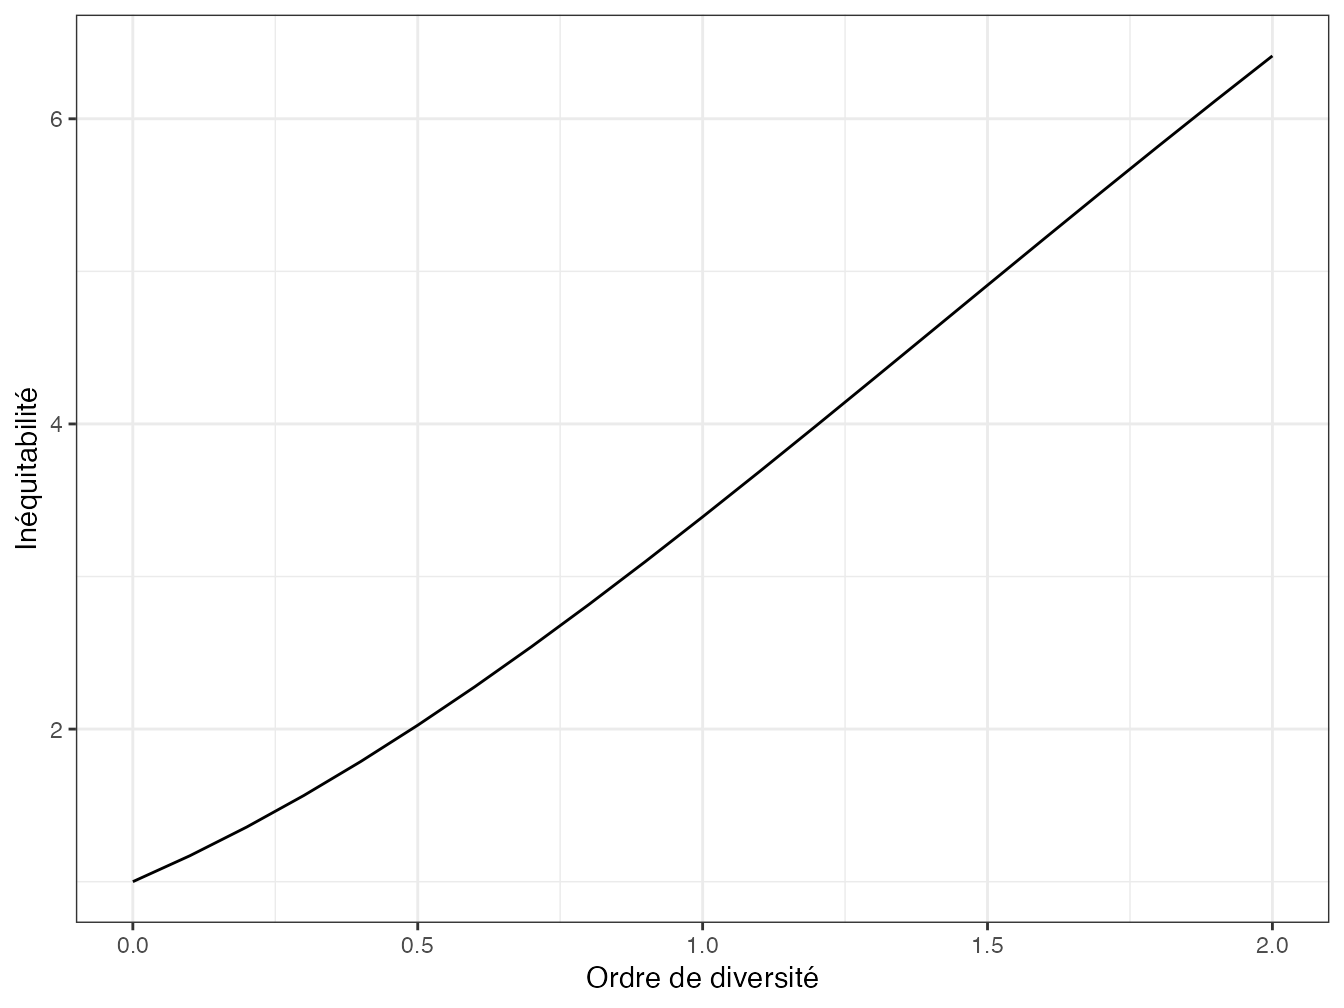
\includegraphics[width=0.8\linewidth]{MesuresBD_files/figure-latex/ProfilIneqFig-1} 

}

\caption{Profil d'inéquitabilité de BCI: L'inéquitabilité augmente quand on néglige de plus en plus les espèces rares. Pour q=2, la forêt de BCI est aussi inéquitable qu'une communauté de 6 espèces dans laquelle une seule serait représentée au-delà d'un nombre négligeable d'individus.}\label{fig:ProfilIneqFig}
\end{SCfigure}

\normalsize

\textcite{Jost2010} montre que l'indépendance est impossible dans le cadre de la décomposition multiplicative: si \(^{q}\!E={^{q}\!D/{S}}\), sa valeur minimale est contrainte par le nombre d'espèces, une communauté pauvre ne peut pas être aussi inéquitable qu'une communauté riche (propriété déjà montrée par \textcite{Sheldon1969} ou \textcite{Alatalo1981}).
En revanche, la richesse peut être partitionnée de façon indépendante en diversité et inéquitabilité: \(S={^{q}\!D}/{^{q}\!E}\).

L'inéquitabilité \(1/{^{q}\!E}\) (figure \ref{fig:ProfilIneqFig}) est un nombre effectif d'espèces: c'est la richesse d'une communauté du même niveau d'équitabilité que la communauté réelle dans laquelle tous les individus (sauf un nombre négligeable) appartiendraient à une seule espèce.

Code R pour la figure \ref{fig:ProfilIneqFig}:

\scriptsize

\begin{Shaded}
\begin{Highlighting}[]
\CommentTok{# Estimation du nombre d'espèces}
\NormalTok{Ns <-}\StringTok{ }\KeywordTok{colSums}\NormalTok{(BCI)}
\NormalTok{UBNs <-}\StringTok{ }\KeywordTok{jackknife}\NormalTok{(}\KeywordTok{AbdFreqCount}\NormalTok{(Ns), }\DataTypeTok{k =} \DecValTok{1}\NormalTok{)}\OperatorTok{$}\NormalTok{Nhat}
\CommentTok{# Profil}
\NormalTok{Inq <-}\StringTok{ }\NormalTok{DivPrf <-}\StringTok{ }\KeywordTok{CommunityProfile}\NormalTok{(Diversity, Ns)}
\NormalTok{Inq}\OperatorTok{$}\NormalTok{y <-}\StringTok{ }\NormalTok{UBNs}\OperatorTok{/}\NormalTok{DivPrf}\OperatorTok{$}\NormalTok{y}
\KeywordTok{autoplot}\NormalTok{(Inq, }\DataTypeTok{xlab =} \StringTok{"Ordre de diversité"}\NormalTok{, }\DataTypeTok{ylab =} \StringTok{"Inéquitabilité"}\NormalTok{)}
\end{Highlighting}
\end{Shaded}

\normalsize

\hypertarget{synthuxe8se-2}{%
\subsection{Synthèse}\label{synthuxe8se-2}}

L'indice de Pielou est le plus utilisé \autocite{Tuomisto2012} mais n'est pas invariant par réplication parce qu'il ne normalise pas une diversité mais une entropie.
Il est rejeté pour cette raison \autocite{Smith1996,Tuomisto2012} par une partie de la littérature.
\textcite{Jost2010} argumente au contraire en sa faveur: \(^{q}\!E\) dépend de la richesse et ne peut donc pas être comparé entre communautés de richesse différente.
Le logarithme de \(^{q}\!E\) normalisé est une meilleure généralisation de l'indice de Pielou que celle de Mendes et al.:

\begin{equation}
  \label{eq:PielouJq}
  ^{q}\!J
  = \frac{\ln\left({^{q}\!D}\right)}{\ln S}
  = \frac{^{q}\!R}{\ln S}.
\end{equation}

\(^{q}\!J\) varie entre 0 et 1 et est une transformation monotone de \(^{q}\!E\) contrairement au \(^{q}\!J^{*}\) de Mendes et al.~
Il est égal au rapport de l'entropie de Rényi sur le logarithme du nombre d'espèces.

L'estimation de l'équitabilité repose lourdement sur l'estimation du nombre d'espèces, quelle que soit la valeur du paramètre \(q\).
La solution la plus évidente consiste à corriger le mieux possible le biais d'estimation du nombre d'espèces et celui de l'entropie d'ordre \(q\):

\begin{equation}
  \label{eq:EstJq}
  ^q\!{\tilde{J}}= \frac{\ln\left(e_q^{^q{\tilde{H}}} \right)}{\ln\tilde{S}}.
\end{equation}



\scriptsize

\begin{SCfigure}

{\centering 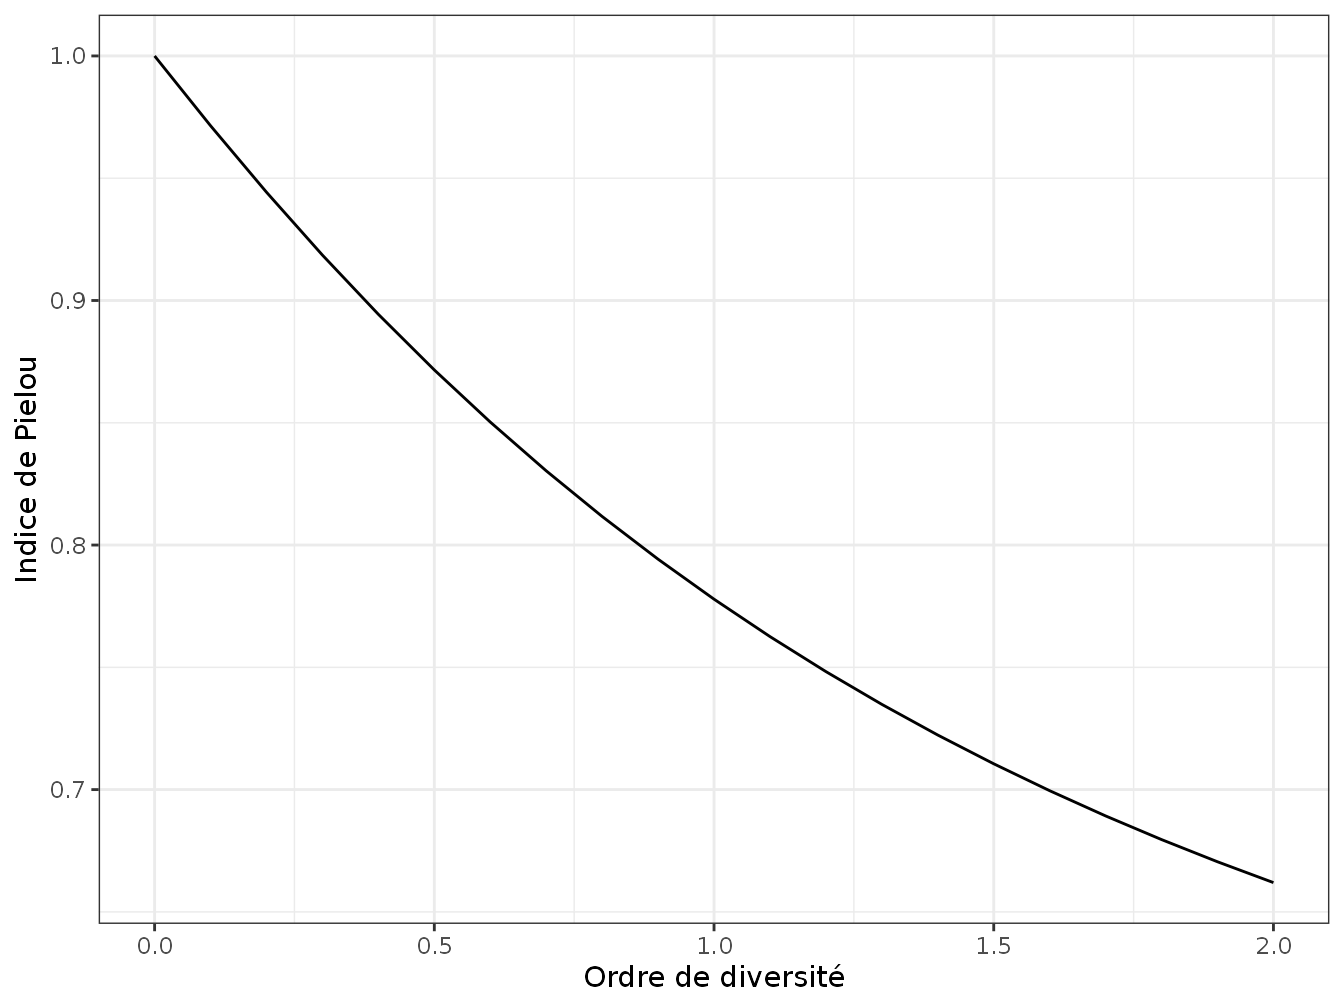
\includegraphics[width=0.8\linewidth]{MesuresBD_files/figure-latex/BCIEqFig-1} 

}

\caption{Profil d'équitabilité de BCI. L'équitabilité est ici normalisée selon Jost.}\label{fig:BCIEqFig}
\end{SCfigure}

\normalsize

Un profil d'équitabilité calculé de cette façon est présenté en figure \ref{fig:BCIEqFig}, représentation alternative de la figure \ref{fig:ProfilIneqFig}.

Code R supplémentaire:

\scriptsize

\begin{Shaded}
\begin{Highlighting}[]
\NormalTok{Inq}\OperatorTok{$}\NormalTok{y <-}\StringTok{ }\KeywordTok{log}\NormalTok{(DivPrf}\OperatorTok{$}\NormalTok{y)}\OperatorTok{/}\KeywordTok{log}\NormalTok{(UBNs)}
\KeywordTok{autoplot}\NormalTok{(Inq, }\DataTypeTok{xlab =} \StringTok{"Ordre de diversité"}\NormalTok{, }\DataTypeTok{ylab =} \StringTok{"Indice de Pielou"}\NormalTok{)}
\end{Highlighting}
\end{Shaded}

\normalsize

\hypertarget{relations-empiriques-entre-richesse-et-uxe9quitabilituxe9}{%
\section{Relations empiriques entre richesse et équitabilité}\label{relations-empiriques-entre-richesse-et-uxe9quitabilituxe9}}

Au-delà de la question des contraintes mathématiques entre richesse et équtabilité traitées précédemment, il s'agit ici des relations entre les deux aspects de la diversité dans des communautés réelles.

\textcite{Wilsey2005} passent en revue l'argument selon lequel richesse et équitabilité seraient toujours positivement corrélés.
S'il est valide, la richesse peut être considérée comme une mesure suffisante de la diversité.
À partir d'inventaires de prairies, ils montrent la très faible relation entre les deux valeurs.
Le suivi temporel de communautés de papillons \autocite{MacDonald2016} met en évidence une relation négative.
Les auteurs de l'étude critiquent un peu naïvement l'utilisation des nombres de Hill pour mesurer la diversité parce qu'ils confondent les effets de la richesse et de l'équitabilité: c'est justement leur but.

D'un point de vue plus théorique, \textcite{DeBenedictis1973} étudie les contraintes numériques sur l'intervalle des valeurs possibles de l'entropie de Shannon et de l'équitabilité en fonction de la richesse.
Il ne prouve pas de corrélation entre ces valeurs pour des communautés réelles mais simplement un lien positif quand les échantillons sont de petite taille et l'effectif minimum de chaque espèce égal à 1: ces contraintes se relâchent si les donnnées sont des probabilités, pouvant tendre vers 0 pour les espèces rares, ou des abondances dans de grands échantillons.
Cette approche est similaire à celle de \textcite{Jost2010}, plus aboutie.

\textcite{May1975} montre que dans le cadre d'une distribution log-normale, la richesse, l'entropie de Simpson et l'équitabilité de Pielou sont positivement corrélées.
Ce résultat a été étendu par \textcite{Stirling2001} aux distributions en log-séries et testé dans des communautés réelles avec des conclusions contrastées, notamment des corrélations négatives ntre richesse et équitabilité dans des communautés très riches.

Des simulations permettent de comprendre les corrélations dans des cas simples.

La figure \ref{fig:SJLogNormaleFig} montre que l'entropie et l'équitabilité sont corrélées positivement à la richesse dans des communautés log-normales de même variance.



\scriptsize

\begin{SCfigure}

{\centering 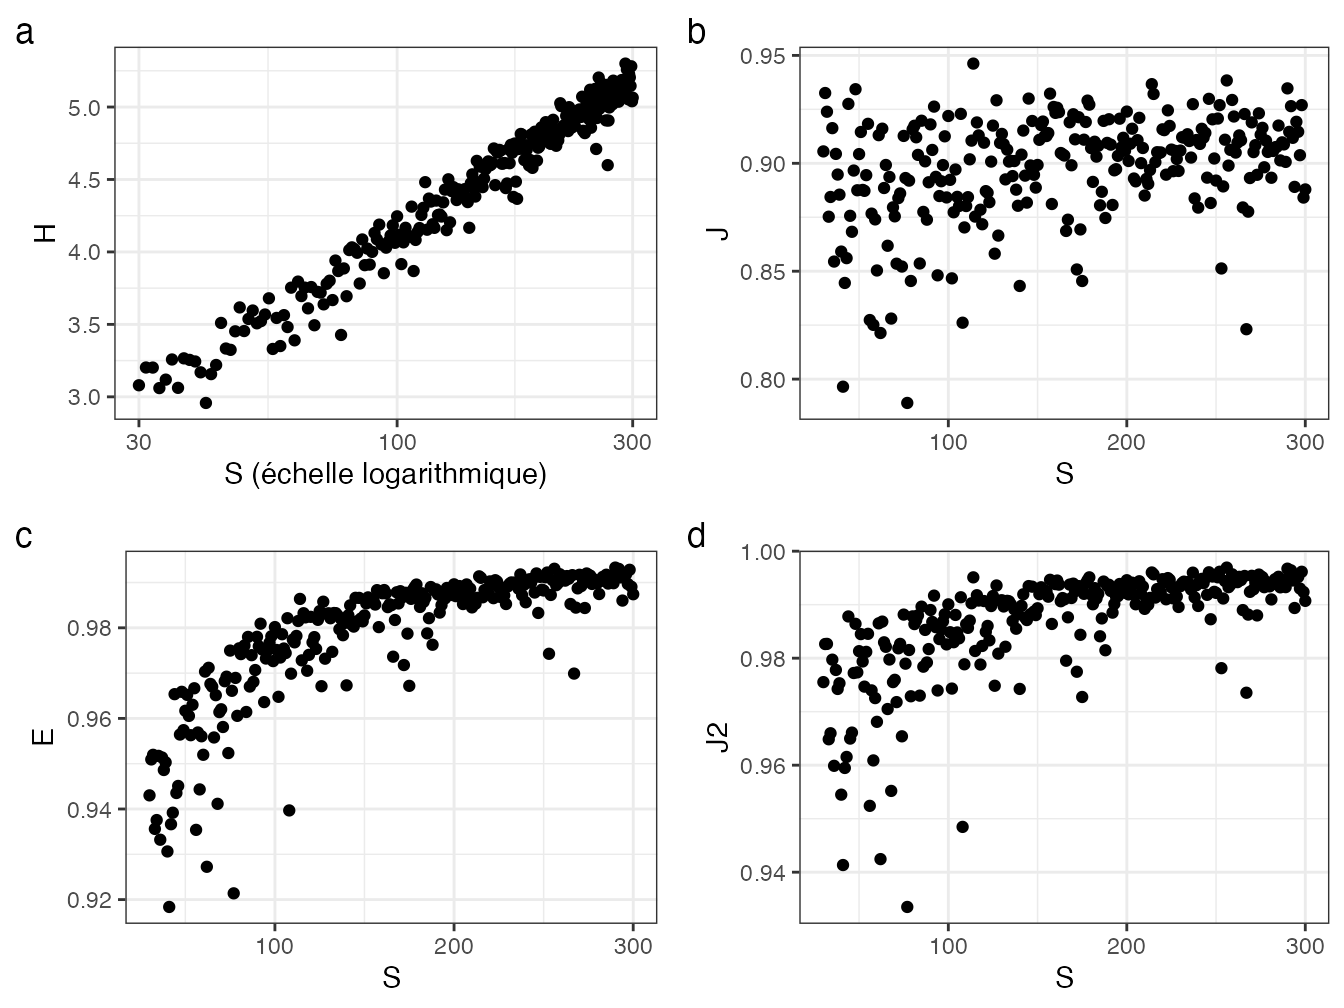
\includegraphics[width=1\linewidth]{MesuresBD_files/figure-latex/SJLogNormaleFig-1} 

}

\caption{Relations entre l'entropie de Shannon (a), l'indice d'équitabilité de Pielou (b), l'entropie de Simpson (c), l'équitabilité de Hurlbert (d) et la richesse de communautés log-normales similaires (même écart-type des probabilités, seule la richesse varie).}\label{fig:SJLogNormaleFig}
\end{SCfigure}

\normalsize

Code R pour réaliser les figures:

\scriptsize

\begin{Shaded}
\begin{Highlighting}[]
\CommentTok{# Communautés de 30 à 300 espèces}
\NormalTok{S <-}\StringTok{ }\DecValTok{30}\OperatorTok{:}\DecValTok{300}
\CommentTok{# Tirage de communautés log-normales de 10000 individus}
\NormalTok{rcl <-}\StringTok{ }\KeywordTok{lapply}\NormalTok{(S, }\ControlFlowTok{function}\NormalTok{(S) }\KeywordTok{rCommunity}\NormalTok{(}\DecValTok{1}\NormalTok{, }\DecValTok{10000}\NormalTok{, }\DataTypeTok{S=}\NormalTok{S))}
\CommentTok{# Richesse et Shannon}
\NormalTok{Sobs <-}\StringTok{ }\KeywordTok{sapply}\NormalTok{(rcl, Richness)}
\NormalTok{H <-}\StringTok{ }\KeywordTok{sapply}\NormalTok{(rcl, Shannon)}
\NormalTok{ggH <-}\StringTok{ }\KeywordTok{ggplot}\NormalTok{(}\KeywordTok{data.frame}\NormalTok{(S, H), }\KeywordTok{aes}\NormalTok{(S, H)) }\OperatorTok{+}
\StringTok{  }\KeywordTok{geom_point}\NormalTok{() }\OperatorTok{+}\StringTok{ }\KeywordTok{scale_x_log10}\NormalTok{() }\OperatorTok{+}\StringTok{ }
\StringTok{  }\KeywordTok{labs}\NormalTok{(}\DataTypeTok{x=}\StringTok{"S (échelle logarithmique)"}\NormalTok{) }\OperatorTok{+}
\StringTok{  }\KeywordTok{labs}\NormalTok{(}\DataTypeTok{tag =} \StringTok{"a"}\NormalTok{)}
\CommentTok{# Equitabilité de Pielou}
\NormalTok{J <-}\StringTok{ }\NormalTok{H}\OperatorTok{/}\KeywordTok{log}\NormalTok{(S)}
\NormalTok{ggJ <-}\StringTok{ }\KeywordTok{ggplot}\NormalTok{(}\KeywordTok{data.frame}\NormalTok{(S, J), }\KeywordTok{aes}\NormalTok{(S, J)) }\OperatorTok{+}
\StringTok{  }\KeywordTok{geom_point}\NormalTok{() }\OperatorTok{+}\StringTok{ }\KeywordTok{labs}\NormalTok{(}\DataTypeTok{tag =} \StringTok{"b"}\NormalTok{)}
\NormalTok{E <-}\StringTok{ }\KeywordTok{sapply}\NormalTok{(rcl, Simpson)}
\NormalTok{ggE <-}\StringTok{ }\KeywordTok{ggplot}\NormalTok{(}\KeywordTok{data.frame}\NormalTok{(S, E), }\KeywordTok{aes}\NormalTok{(S, E)) }\OperatorTok{+}
\StringTok{  }\KeywordTok{geom_point}\NormalTok{() }\OperatorTok{+}\StringTok{ }\KeywordTok{labs}\NormalTok{(}\DataTypeTok{tag =} \StringTok{"c"}\NormalTok{)}
\NormalTok{J2 <-}\StringTok{ }\NormalTok{E}\OperatorTok{/}\NormalTok{(}\DecValTok{1-1}\OperatorTok{/}\NormalTok{S)}
\NormalTok{ggJ2 <-}\StringTok{ }\KeywordTok{ggplot}\NormalTok{(}\KeywordTok{data.frame}\NormalTok{(S, J2), }\KeywordTok{aes}\NormalTok{(S, J2)) }\OperatorTok{+}
\StringTok{  }\KeywordTok{geom_point}\NormalTok{() }\OperatorTok{+}\StringTok{ }\KeywordTok{labs}\NormalTok{(}\DataTypeTok{tag =} \StringTok{"d"}\NormalTok{)}
\KeywordTok{grid.arrange}\NormalTok{(ggH, ggJ, ggE , ggJ2, }\DataTypeTok{ncol =} \DecValTok{2}\NormalTok{, }\DataTypeTok{nrow =} \DecValTok{2}\NormalTok{)}
\end{Highlighting}
\end{Shaded}

\normalsize

En revanche, dans une communauté log-normale de richesse fixe mais insuffisamment échantillonnée, les corrélations sont négatives (figure \ref{fig:NJLogNormaleFig}).
Le sous-échantillonnage a un effet plus sévère sur la richesse que sur les entropies d'ordres supérieurs.
La non observation des espèces les plus rares augmente aussi l'équitabilité.



\scriptsize

\begin{SCfigure}

{\centering 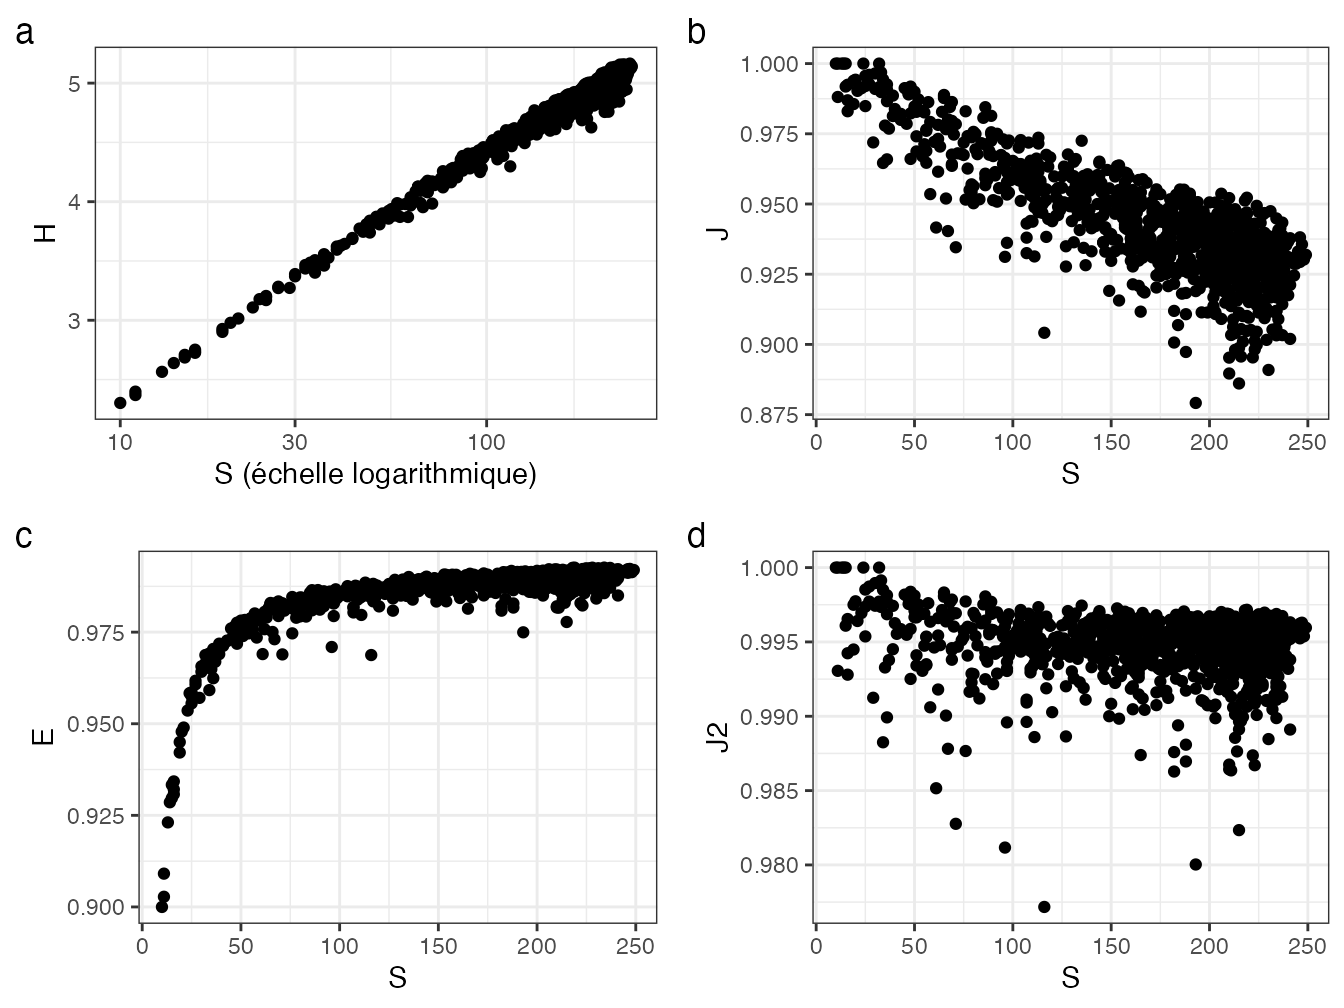
\includegraphics[width=1\linewidth]{MesuresBD_files/figure-latex/NJLogNormaleFig-1} 

}

\caption{Relations entre l'entropie de Shannon (a), l'indice d'équitabilité de Pielou (b), l'entropie de Simpson (c), l'équitabilité de Hurlbert (d) et la richesse d'échantillons de taille variable d'une même communauté log-normale.}\label{fig:NJLogNormaleFig}
\end{SCfigure}

\normalsize

Code R pour réaliser les figures:

\scriptsize

\begin{Shaded}
\begin{Highlighting}[]
\CommentTok{# Communautés de taille 10 à 1000 individus; 300 sp.}
\NormalTok{rmc <-}\StringTok{ }\KeywordTok{MetaCommunity}\NormalTok{(}\KeywordTok{sapply}\NormalTok{(}\DecValTok{10}\OperatorTok{:}\DecValTok{1000}\NormalTok{, }\ControlFlowTok{function}\NormalTok{(n) }\KeywordTok{rCommunity}\NormalTok{(}\DecValTok{1}\NormalTok{, n)))}
\CommentTok{# Richesse et Shannon}
\NormalTok{S <-}\StringTok{ }\KeywordTok{apply}\NormalTok{(rmc}\OperatorTok{$}\NormalTok{Psi, }\DecValTok{2}\NormalTok{, Richness)}
\NormalTok{H <-}\StringTok{ }\KeywordTok{apply}\NormalTok{(rmc}\OperatorTok{$}\NormalTok{Psi, }\DecValTok{2}\NormalTok{, Shannon)}
\NormalTok{ggH <-}\StringTok{ }\KeywordTok{ggplot}\NormalTok{(}\KeywordTok{data.frame}\NormalTok{(S, H), }\KeywordTok{aes}\NormalTok{(S, H)) }\OperatorTok{+}
\StringTok{  }\KeywordTok{geom_point}\NormalTok{() }\OperatorTok{+}\StringTok{ }\KeywordTok{scale_x_log10}\NormalTok{() }\OperatorTok{+}\StringTok{ }
\StringTok{  }\KeywordTok{labs}\NormalTok{(}\DataTypeTok{x=}\StringTok{"S (échelle logarithmique)"}\NormalTok{) }\OperatorTok{+}
\StringTok{  }\KeywordTok{labs}\NormalTok{(}\DataTypeTok{tag =} \StringTok{"a"}\NormalTok{)}
\CommentTok{# Equitabilité de Pielou}
\NormalTok{J <-}\StringTok{ }\NormalTok{H}\OperatorTok{/}\KeywordTok{log}\NormalTok{(S)}
\NormalTok{ggJ <-}\StringTok{ }\KeywordTok{ggplot}\NormalTok{(}\KeywordTok{data.frame}\NormalTok{(S, J), }\KeywordTok{aes}\NormalTok{(S, J)) }\OperatorTok{+}
\StringTok{  }\KeywordTok{geom_point}\NormalTok{() }\OperatorTok{+}\StringTok{ }\KeywordTok{labs}\NormalTok{(}\DataTypeTok{tag =} \StringTok{"b"}\NormalTok{)}
\NormalTok{E <-}\StringTok{ }\KeywordTok{apply}\NormalTok{(rmc}\OperatorTok{$}\NormalTok{Psi, }\DecValTok{2}\NormalTok{, Simpson)}
\NormalTok{ggE <-}\StringTok{ }\KeywordTok{ggplot}\NormalTok{(}\KeywordTok{data.frame}\NormalTok{(S, E), }\KeywordTok{aes}\NormalTok{(S, E)) }\OperatorTok{+}
\StringTok{  }\KeywordTok{geom_point}\NormalTok{() }\OperatorTok{+}\StringTok{ }\KeywordTok{labs}\NormalTok{(}\DataTypeTok{tag =} \StringTok{"c"}\NormalTok{)}
\NormalTok{J2 <-}\StringTok{ }\NormalTok{E}\OperatorTok{/}\NormalTok{(}\DecValTok{1-1}\OperatorTok{/}\NormalTok{S)}
\NormalTok{ggJ2 <-}\StringTok{ }\KeywordTok{ggplot}\NormalTok{(}\KeywordTok{data.frame}\NormalTok{(S, J2), }\KeywordTok{aes}\NormalTok{(S, J2)) }\OperatorTok{+}
\StringTok{  }\KeywordTok{geom_point}\NormalTok{() }\OperatorTok{+}\StringTok{ }\KeywordTok{labs}\NormalTok{(}\DataTypeTok{tag =} \StringTok{"d"}\NormalTok{)}
\KeywordTok{grid.arrange}\NormalTok{(ggH, ggJ, ggE , ggJ2, }\DataTypeTok{ncol =} \DecValTok{2}\NormalTok{, }\DataTypeTok{nrow =} \DecValTok{2}\NormalTok{)}
\end{Highlighting}
\end{Shaded}

\normalsize

La corrélation entre richesse et équitabilité est donc positive si la richesse varie entre communautés, mais négative si ce n'est qu'un effet de l'échantillonnage.
Les résultats sont similaires avec des communautés en log-séries: la corrélation est positive quand \(\alpha\) varie, négative quand l'échantillonnage varie.

\hypertarget{part-diversituxe9-fonctionnelle-et-phyloguxe9nuxe9tique}{%
\part{Diversité fonctionnelle et phylogénétique}\label{part-diversituxe9-fonctionnelle-et-phyloguxe9nuxe9tique}}

\hypertarget{cadre}{%
\chapter{Cadre}\label{cadre}}

\scriptsize

\normalsize

\scriptsize

\begin{Essentiel}
La diversité fonctionnelle ou phylogénétique prend en compte la
proximité des espèces entre elles. Généralement, la distance entre
espèces est évaluée dans l'espace des traits, approximation de l'espace
des niches, pour la diversité fonctionnelle et dans un dendrogramme
représentant la phylogénie ou la taxonomie pour la diversité
phylogénétique.
\end{Essentiel}

\normalsize

Les mesures neutres de la diversité considèrent que toutes les classes auxquelles les objets appartiennent sont différentes, sans que certaines soient plus différentes que d'autres.
Par exemple, toutes les espèces sont équidistantes les unes des autres, qu'elles appartiennent au même genre ou à des familles différentes.
Intuitivement, l'idée qu'une communauté de \(S\) espèces toutes de genres différents est plus diverse qu'une communauté de \(S\) espèces du même genre est satisfaisante.
\textcite{Walker1992} argumente en faveur de la protection de groupes fonctionnels plutôt que de celle de chacune des espèces qui les constitue pour maintenir le bon état des écosystèmes.

Il s'agit donc de caractériser la différence entre deux classes d'objets, puis de construire des mesures de diversité en rapport \autocite{Pielou1975,May1990a,Cousins1991}.
En écologie, ces différences sont fonctionnelles ou phylogénétiques, définissant la diversité fonctionnelle \autocite{Tilman1997} ou la diversité phylogénétique (\emph{phylodiversity}) \autocite{Webb2006}.

Les premières propositions de ce type d'indices sont dues à \textcite{Rao1982} (voir section \ref{sec:Rao}) puis, avec nettement moins de succès, \textcite{Vane-Wright1991} et \textcite{Warwick1995}.
\textcite{Chave2007} montrent que la diversité neutre prédit mal la diversité phylogénétique (calculée par l'entropie quadratique de Rao).

De nombreuses mesures de diversité ont été créées et plusieurs revues permettent d'en faire le tour. \autocite{Ricotta2007,Vellend2010}
Les mesures présentées ici sont les plus utilisées, et notamment celles qui peuvent être ramenées aux mesures classiques en fixant une distance égale entre toutes les espèces.
Le cadre méthodologique dans lequel ces mesures ont été développées est présenté dans ce chapitre, suivi par une revue des nombreuses mesures de diversité fonctionnelles et phylogénétiques de la littérature.
L'entropie phylogénétique et la diversité de Leinster et Cobbold sont ensuite développées en détail, suivies d'une synthèse et de considérations sur la mesure de la diversité individuelle plutôt que spécifique.

Des exemples montrent comment calculer cette diversité, principalement à l'aide du package \emph{entropart}.
Le package contient les données d'inventaire de deux hectares du dispositif de Paracou et la taxonomie des espèces concernées:

\scriptsize

\begin{Shaded}
\begin{Highlighting}[]
\KeywordTok{library}\NormalTok{(}\StringTok{"entropart"}\NormalTok{)}
\CommentTok{# Chargement du jeu de données}
\KeywordTok{data}\NormalTok{(Paracou618)}
\end{Highlighting}
\end{Shaded}

\normalsize

\hypertarget{dissimilarituxe9-et-distance}{%
\section{Dissimilarité et distance}\label{dissimilarituxe9-et-distance}}

Une similarité ou dissimilarité est toute application à valeurs numériques qui permet de mesurer le lien entre les individus d'un même ensemble ou entre les variables.
Pour une similarité le lien est d'autant plus fort que sa valeur est grande.

Une dissimilarité vérifie (\(k\), \(l\) et \(m\) sont trois individus):

\begin{itemize}
\tightlist
\item
  La dissimilarité d'un individu avec lui-même est nulle: \(d\left(k,k\right)=0\);
\item
  La dissimilarité entre deux individus différents est positive: \(d\left(k,l\right)\ge 0\);
\item
  La dissimilarité est symétrique: \(d\left(k,l\right)=d\left(l,k\right)\).
\end{itemize}

Une distance vérifie en plus:

\begin{itemize}
\tightlist
\item
  La distance entre deux individus différents est strictement positive: \(d\left(k,l\right)=0\Rightarrow k=l\);
\item
  L'inégalité triangulaire: \(d\left(k,m\right)\le d\left(k,l\right)+d\left(l,m\right)\).
  De nombreux indices de dissimilarité ne vérifient pas cette propriété.
\end{itemize}

Une distance est euclidienne si elle peut être représentée par des figures géométriques.
On peut rendre toute distance euclidienne par ajout d'une constante \autocite{Lingoes1971,Cailliez1983}.
Dans R, utiliser \texttt{is.euclid()} pour vérifier qu'une distance est euclidienne, et \texttt{cailliez()} ou \texttt{lingoes()} pour la transformation.

Enfin, une distance est ultramétrique si \(d\left(k,m\right) \le \max\left(d\left(k,l\right),d\left(l,m\right)\right)\).
Les distances obtenues en mesurant les longueurs des branches d'un dendrogramme (arbre) résultant d'une classification hiérarchique sont ultramétriques.



\scriptsize

\begin{SCfigure}

{\centering 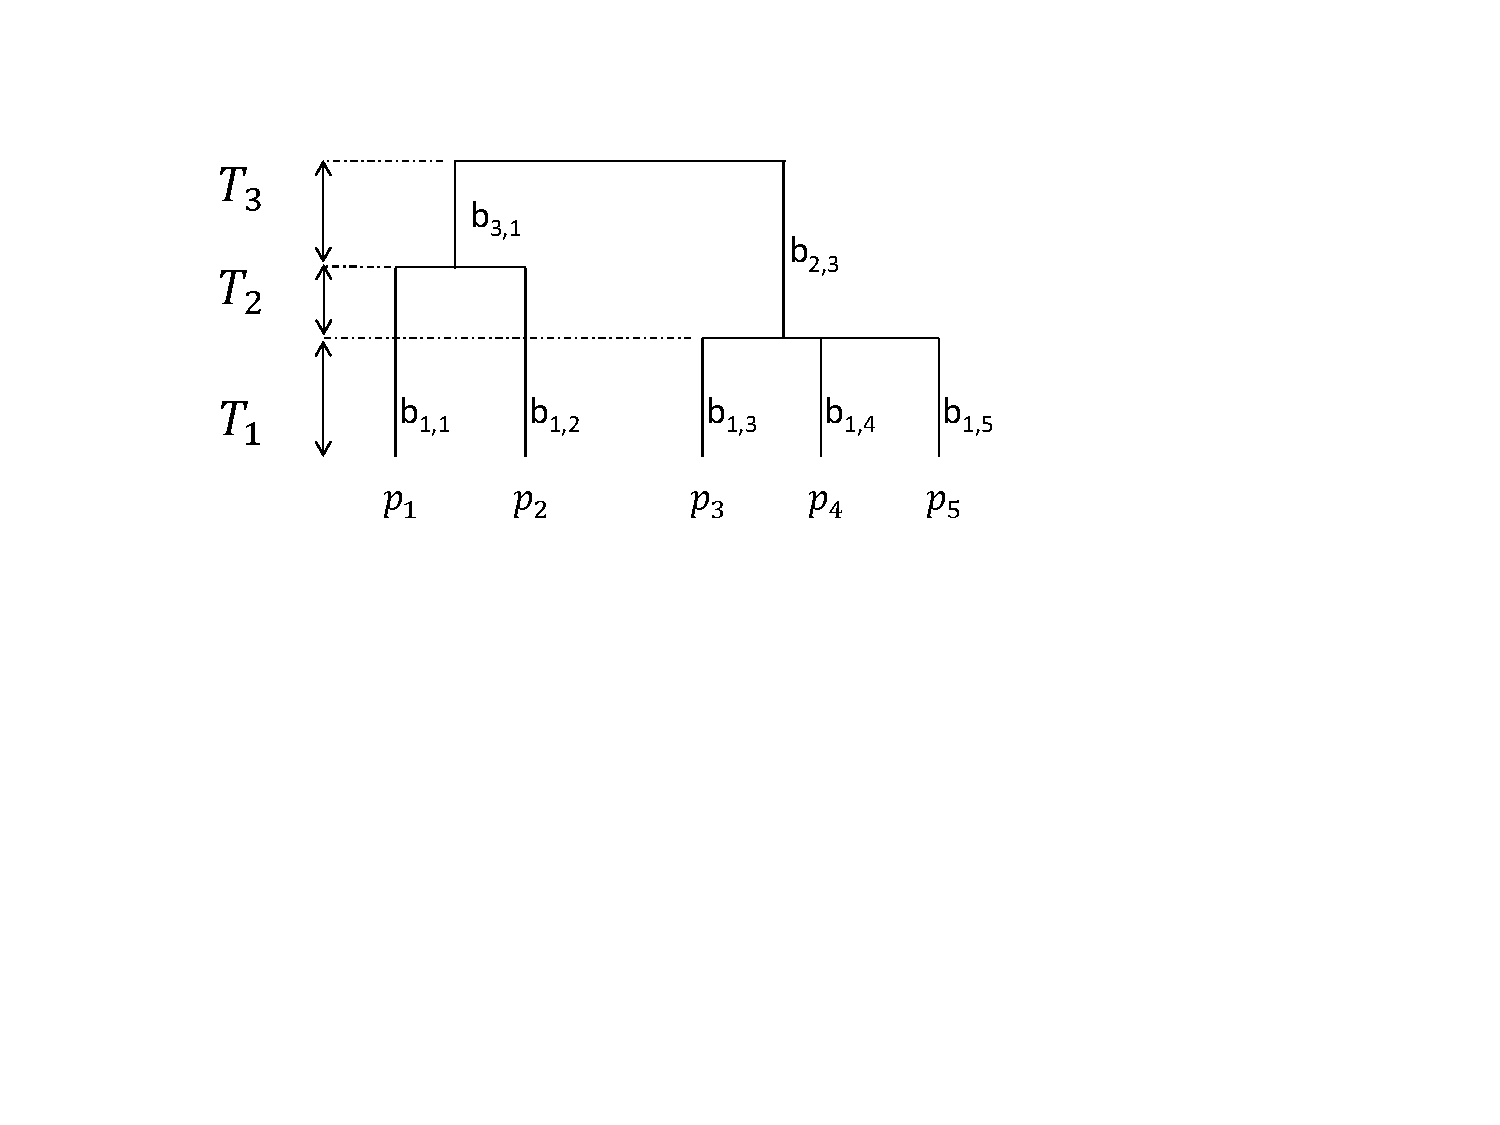
\includegraphics[width=0.8\linewidth]{images/ArbreA} 

}

\caption{Arbre phylogénétique ou fonctionnel hypothétique. 5 espèces sont présentes (\(S=5\)), leurs probabilités notées \(p_1\) à \(p_5\). Les noms des branches sont affichés.}\label{fig:ArbreA1}
\end{SCfigure}

\normalsize

La façon exacte de mesurer les longueurs de branche est illustrée par la figure \ref{fig:ArbreA1}: la distance entre les espèces 1 et 2 est \(T_1+T_2\), elle est égale à \(T_1\) entre les espèces 4 et 5.
La distance est la hauteur du premier noeud commun.

\hypertarget{sec:Dphylo}{%
\section{Distance phylogénétique}\label{sec:Dphylo}}

La façon la plus évidente de définir une distance entre espèces est d'utiliser la taxonomie \autocite[Warwick2001]{Clarke2001}, en attribuant une distance arbitraire (par exemple 1) à deux espèces du même genre, une autre (par exemple 2) à deux espèces de la même famille, etc.
La distance définie est ultramétrique.

La taxonomie peut être remplacée avantageusement par une phylogénie.
La phylogénie idéale contiendrait l'histoire évolutive de toutes les espèces et les distances seraient les temps de divergence depuis le premier ancêtre commun.
En pratique, les phylogénies sont établies à partir d'un nombre de marqueurs génétiques limités, sans datation précise (mais avec des calages partiels à partir de fossiles), et ne sont pas toujours ultramétriques.
Elles peuvent prendre en compte chaque individu, sans regroupement par espèce.
Une méthode pour dater une phylogénie est fournie par \textcite{Chave2007}
\textcite{Zanne2014} fournissent une phylogénie datée de plus de 32000 espèces.
\textcite{Ricotta2012a} montrent sur des exemples que la diversité calculée à partir de phylogénies datées est très corrélée à celle calculée à partir de simples taxonomies.

Dans tous les cas, la distance est une mesure de la divergence évolutive.
Du point de vue de la biologie de la conservation, chaque espèce accumule une quantité d'évolution, interprétée comme une quantité d'information \autocite{Crozier1997} dont le maximum doit être préservé.

L'entropie phylogénétique (voir chapitre \ref{chap:Phyloentropie}) utilise un arbre phylogénétique pour mesurer la diversité.

\hypertarget{sec:DFonctionnelle}{%
\section{Distance fonctionnelle}\label{sec:DFonctionnelle}}

L'approche fonctionnelle est différente.
Chaque espèce ou individu est représenté par ses valeurs de traits dans un espace multidimensionnel.
Le vecteur de traits est considéré comme un proxy de la niche écologique \autocite{Westoby2002}.
Les individus proches dans l'espace des traits sont donc considérés comme proches écologiquement.
Les distances entre les points peuvent être calculées directement dans l'espace des traits ou, fréquemment, un arbre est construit par classification automatique hiérarchique.

La première étape consiste donc à choisir un ensemble de traits pertinents et à les mesurer de façon standardisée \autocite{Cornelissen2003}.
Toute la stratégie relative à la photosynthèse peut être par exemple assez bien résumée par la masse surfacique des feuilles \autocite{Wright2004}, mais, en forêt tropicale, ce trait est décorrélé de la densité du bois \autocite{Baraloto2010}.
Les valeurs manquantes peuvent être complétées en utilisant toute l'information disponible par MICE (\emph{multiple imputation by chained equations}) \autocite{VanBuuren2006}, disponible sous R dans le package \texttt{mice} \autocite{VanBuuren2011}.

La prise en compte de variables qualitatives ou de rang et la possibilité de données manquantes pose un problème pratique de construction de la matrice de dissimilarité, traité par \textcite{Gower1971}.
La formule de Gower, étendue par \textcite{Podani1999} puis \textcite{Pavoine2009b} à d'autres types de variables, calcule la dissimilarité entre deux espèces par la moyenne des dissimilarités calculées pour chaque trait, dont la valeur est comprise entre 0 et 1:

\begin{itemize}
\tightlist
\item
  Pour une variable quantitative, la différence de valeur entre deux espèces est normalisée par l'étendue des valeurs de la variable;
\item
  Les variables ordonnées sont remplacées par leur rang et traitées comme les variables quantitatives;
\item
  Pour des variables qualitatives, la dissimilarité vaut 0 ou 1;
\item
  Les valeurs manquantes sont simplement ignorées et n'entrent pas dans la moyenne.
\end{itemize}

Une matrice de distances entre espèces est construite de cette façon.
\textcite{Podani2006} suggèrent d'utiliser ensuite une classification hiérarchique par UPGMA \autocite{Sokal1958} qu'ils montrent être la plus robuste (pour le calcul de FD, voir section \ref{sec:PDFD}) à l'ajout ou au retrait d'un trait ou d'une espèce.
\textcite{Mouchet2008} suggèrent plutôt d'appliquer toutes les méthodes de classification et de retenir à la fin l'arbre dont la distribution des distances entre espèces dans l'arbre est la plus proche de la distribution des distances dans la matrice de dissimilarités: cette proximité est mesurée par la corrélation cophénétique, c'est-à-dire le coefficient de corrélation entre les valeurs de distances \autocite{Sokal1962,Legendre2012}.
Un arbre consensus \autocite{Felsenstein2004} est souvent plus proche de la matrice de distance.

Un dendrogramme fonctionnel n'a pas d'interprétation aussi claire qu'un arbre phylogénétique qui représente le processus de l'évolution.
Il peut être interprété comme la représentation à des échelles de plus en plus grossières en allant vers le haut de l'arbre de regroupements fonctionnels dans des niches de plus en plus vastes.

La transformation d'une matrice (non ultramétrique) en dendrogramme déforme la topologie des espèces \autocite{Pavoine2005a,Podani2007}: une mesure de diversité qui utilise directement la matrice est préférable, c'est un intérêt de la diversité de Leinster et Cobbold (voir chapitre \ref{chap:LeinsterCobbold}).
\textcite{Maire2015} ont défini une mesure de qualité d'un espace fonctionnel, \emph{mSD}, comme l'écart quadratique moyen entre les distances fonctionnelles entre espèces dans l'espace utilisé (par exemple les distances cophénétiques dans un dendrogramme fonctionnel) et les distances originales (dans la matrice de distance à partir de laquelle l'arbre a été obtenu).
Dans la matrice originale, les valeurs de traits sont centrées et réduites, et la hauteur du dendrogramme est fixée pour que la distance cophénétique maximale soit égale à la distance originale maximale.

\textcite{Villeger2017} ont montré que l'utilisation de dendrogrammes fonctionnels dans une étude de \textcite{Sobral2016} amène à sous-estimer les changements de niveau de biodiversité liés à l'arrivée d'espèces invasives d'oiseaux.
Dans la très grande majorité des dendrogrammes utilisés, la transformation de la matrice de distance a entraîné un écart moyen de plus de 10\% par rapport aux valeurs originales (une valeur de \emph{mSD}, l'écart quadratique moyen, supérieure à 1\%).
Cette déformation est suffisante pour largement invalider les résultats obtenus.

\hypertarget{uxe9quivalence-des-deux-diversituxe9s}{%
\section{Équivalence des deux diversités}\label{uxe9quivalence-des-deux-diversituxe9s}}

L'approche fonctionnelle étant particulièrement complexe et lourde à mettre en oeuvre (notamment pour la mesure des traits sur chaque individu), la tentation a été grande de considérer que la phylogénie contenait plus d'information fonctionnelle que ce qui pouvait être mesuré, et donc de considérer la diversité phylogénétique comme proxy de la diversité fonctionnelle.

Du point de vue théorique, le modèle le plus simple de l'évolution de la valeur d'un trait hypothétique au cours du temps est le mouvement brownien: à chaque génération, la valeur du trait varie un peu, sans mémoire.
Dans ce cadre \autocite{Felsenstein1985}, la variance de la valeur actuelle du trait pour une espèce donnée est proportionnelle à la durée de l'évolution et la covariance entre deux espèces à celle de l'âge de leur ancêtre commun.
Deux espèces proches dans l'arbre phylogénétique décrivant l'évolution doivent donc avoir des valeurs de trait corrélées.

\textcite{Webb2000} a montré que des communautés d'arbres tropicaux avaient une moins grande diversité phylogénétique locale qu'attendue sous l'hypothèse nulle d'une distribution aléatoire des espèces, et a supposé que la cause en était le filtrage environnemental local, agissant sur les traits et observables par la phylogénie, sous l'hypothèse de conservation phylogénétique des traits fonctionnels.
La discipline appelée \emph{écologie phylogénétique des communautés} cherche encore à comprendre quels traits sont conservés et lesquels sont convergents \autocite{Cavender-Bares2009}.

\textcite{Swenson2009} ont montré que la relation entre les deux diversités était faible.
L'utilisation de la diversité phylogénétique comme proxy de la diversité fonctionnelle n'est pas satisfaisante \autocite{Pavoine2011}. Pour optimiser la conservation, les deux aspects de la diversité, souvent divergents, doivent être pris en compte \autocite{Devictor2010}.

\hypertarget{typologie-des-mesures}{%
\section{Typologie des mesures}\label{typologie-des-mesures}}

À partir de la littérature \autocite{Ricotta2007,Pavoine2011}, une typologie des mesures de diversité émerge.
Elle étend les notions classiques de richesse et équitabilité.

La richesse est l'accumulation de classes différentes dans les mesures classiques.
Dans un arbre phylogénétique, la longueur des branches représente un temps d'évolution: la richesse en est la somme.
FD et PD sont des mesures de richesse.



\scriptsize

\begin{SCfigure}

{\centering 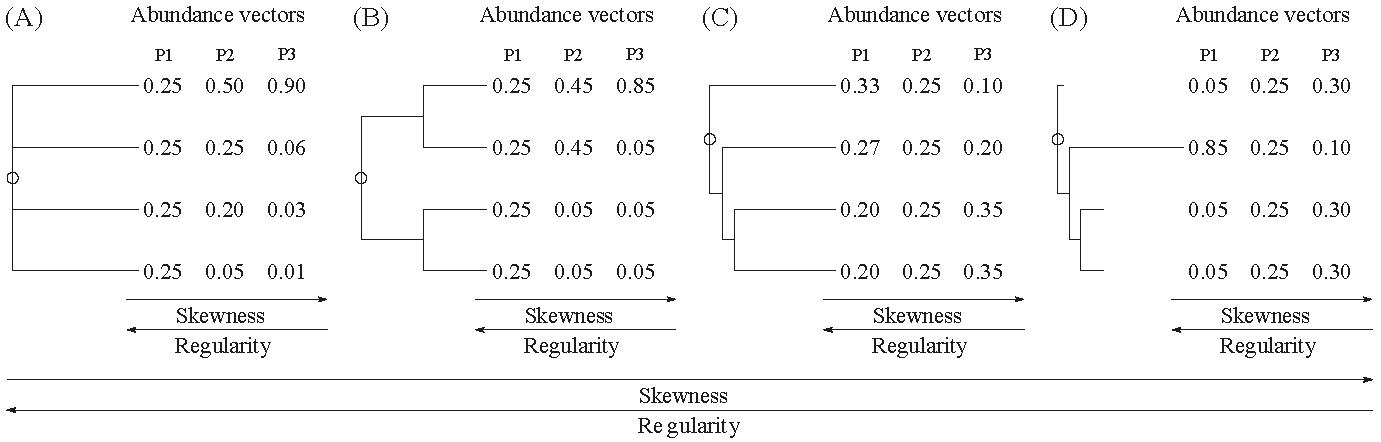
\includegraphics[width=0.8\linewidth]{images/Pavoine2011} 

}

\caption{Régularité contre irrégularité. Les arbres de A à D sont de plus en plus irréguliers. L'arbre A, parfaitement régulier, est le cadre des mesures classiques de la diversité. La phylogénie étant donnée, trois vecteurs d'abondance (P1 à P3) sont de moins en moins réguliers: dans les cas C et D, la régularité maximale n'est pas obtenue pour des effectifs identiques, mais en augmentant les effectifs des espèces originales.}\label{fig:Pavoine2011}
\end{SCfigure}

\normalsize

La régularité mesure la façon dont les espèces occupent uniformément l'espace des niches \autocite{Pavoine2011}.
Cette notion est simple dans un espace multidimensionnel (par exemple, l'espace des traits fonctionnels).
Dans un arbre phylogénétique (figure \ref{fig:Pavoine2011}, \textcite{Pavoine2011}), la régularité de l'arbre \autocite{Mooers1997} est un premier critère, complété éventuellement par les abondances.
Dans un arbre parfaitement régulier, la régularité se réduit à l'équitabilité.

Les mesures de divergence sont des fonctions croissantes de la dissimilarité entre les espèces, généralement considérées par paires.
Certaines sont pondérées par les abondances, d'autres non.
Dans un arbre parfaitement régulier, l'indice de Simpson est une mesure de divergence pondérée.
Ces mesures sont influencées par la richesse et la régularité.

Face à la profusion des mesures de diversité fonctionnelle, \textcite{Ricotta2005d}, en complément de \textcite{Solow1994} établit un certain nombre d'axiomes:

\begin{enumerate}
\def\labelenumi{\arabic{enumi}.}
\tightlist
\item
  Monotonicité d'ensemble: la diversité ne doit pas diminuer quand une espèce est ajoutée avec une faible probabilité (qui ne modifie pas la structure de la communauté existante), quelles que soient ses caractéristiques fonctionnelles;
\item
  Jumelage \autocite{Weitzman1992}: l'introduction d'une espèce identique à une espèces existante ne doit pas augmenter la diversité. De façon moins triviale, une espèce infiniment proche ne doit pas augmenter la diversité: il s'agit donc d'un axiome de continuité dans l'espace des niches.
\item
  Monotonicité de distance: la diversité ne doit pas diminuer quand la distance entre espèces est augmentée.
\item
  Décomposabilité: les mesures de divergence doivent être décomposables en diversité \(\alpha\), \(\beta\) et \(\gamma\), ce qui implique leur concavité par rapport aux probabilités.
\end{enumerate}

L'entropie phylogénétique permet d'unifier ces notions, mais de nombreuses mesures ont été proposées.
Elles sont détaillées au chapitre suivant.

\hypertarget{mesures-particuliuxe8res}{%
\chapter{Mesures particulières}\label{mesures-particuliuxe8res}}

\scriptsize

\begin{Essentiel}
De nombreuses mesures de diversité fonctionnelle ou phylogénétique ont
été développées pour combiner le mieux possible la richesse et la
régularité de la distribution des espèces dans l'espace des niches ou la
phylogénie. Certaines (PD, FD, l'entropie quadratique de Rao, \(H_p\) et
\(I_1\)) seront unifiées au chapitre suivant dans le cadre de l'entropie
phylogénétique.
\end{Essentiel}

\normalsize

Un certain nombre de mesures de diversité phylogénétiques a émergé dans la littérature.
Elles sont passées en revue ici, en commençant par la diversité fonctionnelle envisagée dans l'espace multidimensionnel des traits.
Les sections suivantes envisagent les espèces dans un arbre phylogénétique.

\hypertarget{richesse-uxe9quitabilituxe9-et-divergence-fonctionnelle}{%
\section{Richesse, équitabilité et divergence fonctionnelle}\label{richesse-uxe9quitabilituxe9-et-divergence-fonctionnelle}}

\textcite{Mason2005} postulent que la diversité fonctionnelle peut être abordée dans trois dimensions indépendantes (\textcite{Jost2010} montrera que l'indépendance n'est pas assurée):

\begin{itemize}
\tightlist
\item
  la richesse fonctionnelle, qui indique l'étendue de l'espace des niches fonctionnelles occupé par la communauté;
\item
  l'équitabilité de la distribution des espèces dans ces niches (appelée régularité par \textcite{Pavoine2011});
\item
  la divergence fonctionnelle, qui mesure comment la distribution des espèces dans l'espace des niches maximise la variabilité des caractéristiques fonctionnelles dans la communauté et combine richesse et équitabilité.
\end{itemize}

\textcite{Schleuter2010} font une revue des mesures utilisées dans ce cadre.
Les notations des indices utilisées ici sont les leurs.

Différents traits numériques sont connus pour toutes les espèces de la communauté.
La matrice \(\mathbf{X}\) les contient: l'élément \(x_{t,s}\) est la valeur moyenne du trait \(t\) pour l'espèce \(s\).
On note \(\mathbf{T}_s\) le vecteur des valeurs moyennes de chaque trait de l'espèce \(s\).

\hypertarget{richesse-fonctionnelle}{%
\subsection{Richesse fonctionnelle}\label{richesse-fonctionnelle}}

\hypertarget{uxe9tendue-fonctionnelle}{%
\subsubsection{Étendue fonctionnelle}\label{uxe9tendue-fonctionnelle}}

L'étendue fonctionnelle \autocite{Mason2005} mesure l'étendue des valeurs d'un trait occupée par une communauté, normalisée par l'étendue maximale possible:
\begin{equation}
  \label{eq:FRR}
  \mathit{FR}_R = \dfrac{\max_s(x_{t,s}) - \min_s(x_{t,s})}{X_{t,max} - X_{t,min}},
\end{equation}

où \(\max_s(x_{t,s})\) est la valeur maximale pour toutes les espèces de la matrice de la valeur du trait \(t\), \(X_{t,max}\) est sa valeur maximale absolue (les notations sont identiques pour les minima).
Les extrêmes absolus peuvent être ceux de l'ensemble des communautés comparées.
Ils sont toujours sous-estimés: il est toujours possible théoriquement de trouver des valeurs plus extrêmes en augmentant l'effort d'échantillonnage.
L'étendue fonctionnelle peut être moyennée sur plusieurs traits.

Schleuter et al.~développent l'indice \(\mathit{FR}_{Is}\) pour prendre en compte la variabilité intraspécifique et les valeurs de traits non occupées par des espèces dans l'étendue fonctionnelle.
Les valeurs de traits individuelles sont nécessaires: l'étendue des valeurs d'un trait est définie comme l'union des étendues des valeurs de chaque espèce.



\scriptsize

\begin{SCfigure}

{\centering 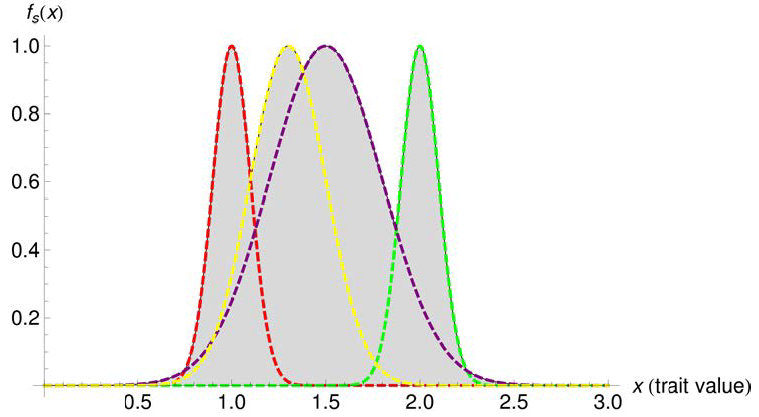
\includegraphics[width=0.8\linewidth]{images/Schleuter2010} 

}

\caption{Fonction d'appartenance de l'espace des niches de Schleuter et al., en une dimension. \(x\), en ordonnée, est la valeur du trait considéré. Chaque espèce est considérée comme un ensemble flou dans l'espace des traits. Quatre espèces sont représentées, avec leur fonction d'appartenance \(f_s(x)\). Le volume de l'espace des traits occupé, \(\mathit{FR}_{Im}\), est obtenu en intégrant les fonctions d'appartenance: c'est la zone grisée de la figure.}\label{fig:Schleuter2010}
\end{SCfigure}

\normalsize

\hypertarget{volume-de-niches}{%
\subsubsection{Volume de niches}\label{volume-de-niches}}

La définition de la niche écologique de \textcite{Hutchinson1957} est l'hypervolume, dans l'espace des ressources environnementales, qu'une espèce peut occuper.
L'espace des traits fonctionnels peut être considéré comme une approximation de l'espace des ressources.
Le volume de l'enveloppe convexe de l'espace des traits occupé par la communauté (\emph{convex hull volume}) est donc une mesure de richesse fonctionnelle multidimensionnelle.
La prise en compte des trous, c'est-à-dire la restriction du volume à l'espace réellement occupé à l'intérieur de cette enveloppe, est possible grâce à une méthode d'estimation d'hypervolume plus élaborée, implémentée dans le package \emph{hypervolume} pour R \autocite{Blonder2014}.

De même que pour l'étendue fonctionnelle, Schleuter et al.~développent une mesure proche, \(\mathit{FR}_{Im}\), prenant en compte la variabilité intraspécifique et les espaces non occupés.
Chaque espèce est supposée occuper un espace autour de sa position moyenne dans l'espace des traits, avec une fonction d'appartenance \autocite{Zadeh1965} gaussienne multidimensionnelle (une représentation unidimensionnelle se trouve en figure \ref{fig:Schleuter2010}, \textcite{Schleuter2010}): la fonction d'appartenance, issue de la logique floue, peut être vue comme une densité de probabilité non normalisée.

Les variances et covariances intraspécifiques des traits (rassemblés dans la matrice carrée \(\mathbf{\Sigma}_s\) de dimension \(t\) pour chaque espèce \(s\)) sont nécessaires.
La fonction d'appartenance de l'espèce \(s\) dans l'espace des traits est, pour le vecteur \(\mathbf{T}\) de valeur de l'ensemble des traits:
\begin{equation}
  f_s(\mathbf{T})= e^{-\frac{1}{2} \left(\mathbf{T}-\mathbf{T}_s \right)^\top \mathbf{\Sigma}_s^{-1}  \left(\mathbf{T}-\mathbf{T}_s \right)}.
\end{equation}

La richesse fonctionnelle est l'intégrale des valeurs maximales de \(f_s\) dans l'ensemble de l'espace des traits:
\begin{equation}
  \label{eq:FRIm}
  \mathit{FR}_{Im} = \int \max_s\left(f_s(\mathbf{T}) \right) \mathop{d\mathbf{T}}.
\end{equation}

Après transformation de la matrice de distance en dendrogramme fonctionnel, éventuellement sous la forme d'un arbre-consensus \autocite{Mouchet2008}, la longueur totale des branches, FD \autocite{Petchey2002}, est une autre mesure de richesse multidimensionnelle.

\hypertarget{equitabilituxe9-fonctionnelle}{%
\subsection{Equitabilité fonctionnelle}\label{equitabilituxe9-fonctionnelle}}

L'équitabilité fonctionnelle, ou régularité \autocite{Pavoine2011}, rend compte de l'homogénéité de l'occupation des niches.

L'indice d'équitabilité de \textcite{Mouillot2005a}, que les auteurs nomment ``indice de régularité fonctionnelle'', est inspiré de l'indice d'équitabilité de Bulla \eqref{eq:Bulla}.
C'est un indice unidimensionnel: un seul trait est pris en compte.
Les espèces sont classées par valeur croissante du trait.
L'équitabilité maximale est obtenue si l'écart entre deux valeurs de traits est proportionnel aux abondances cumulées des deux espèces.
La statistique fondamentale est appelée équitabilité pondérée (\emph{weighted evenness}).
Pour l'intervalle entre l'espèce \(s\) et l'espèce \(s+1\):

\begin{equation}
  \label{eq:EWs}
  \mathit{EW}_{s} = \frac{T_{s+1}-T_{s}}{N_{s+1}+N_{s}}.
\end{equation}

Cette valeur est normalisée: \(\mathit{PEW}_{s}={\mathit{EW}_{s}}/{\sum_s{\mathit{EW}_{s}}}\).
Sa valeur de \(\mathit{PEW}_{s}\) attendue pour le maximum d'équitabilité est \({1}/{(S-1)}\).
L'indice est celui de Bulla, appliqué aux \(S-1\) intervalles entre espèces:

\begin{equation}
  \label{eq:FEs}
  \mathit{FE}_{s} = \sum_{s=1}^{S-1}{\min(\mathit{PEW}_{s},\frac{1}{S-1})}.
\end{equation}

L'indice \(\mathit{FE}_{s}\) a été étendu pour être multidimensionnel par \textcite{Villeger2008a}.
L'arbre recouvrant de longueur minimum (\emph{minimum spanning tree}) est d'abord calculé à partir des distances euclidiennes entre les espèces dans l'espace des traits: il s'agit de l'arbre de longueur totale minimale reliant tous les points.
La longueur des branches est ensuite traitée de la même façon que \(\delta T_s\) précédemment.

Un autre indice, \({\Lambda}^+\) \autocite{Clarke2001}, mesure la variance des distances entre paires d'espèces:

\begin{equation}
  \label{eq:Clarke2001}
  {\Lambda}^+ =\frac{\sum_s{\sum_t{{\left(d_{s,t}-\hat{d}\right)}^2}}}{S\left(S-1\right)}.
\end{equation}

Comme le montrent \textcite{Merigot2011}, les mesures de régularité n'ont absolument pas les mêmes propriétés que les mesures de diversité: elles peuvent par exemple augmenter quand on retire des espèces originales.

\hypertarget{divergence-fonctionnelle}{%
\subsection{Divergence fonctionnelle}\label{divergence-fonctionnelle}}

Les mesures de divergence fonctionnelle décrivent la variabilité de position des espèces dans l'espace des traits.
Ce sont tout simplement des mesures de diversité au sens classique du terme.

Quand un seul trait est considéré, la mesure la plus simple est sa variance.
\textcite{Mason2003} effectuent une transformation logarithmique de la valeur du trait et pondèrent le calcul de la variance par les probabilités \(p_s\).
Ils transforment finalement le résultat en son arc-tangente pour qu'il soit compris entre 0 et 1.

Schleuter et al.~proposent d'utiliser la différence entre le troisième et le premier quartile de la valeur du trait, normalisée par son étendue maximale possible.

FAD a été proposé par \textcite{Walker1999}, à partir d'une matrice de distances dans l'espace des traits.
\(d_{s,t}\) est la distance entre deux espèces indicées par \(s\) et \(t\), alors:

\begin{equation}
  \label{eq:FAD}
  \mathit{FAD}=\sum_s{\sum_t{d_{s,t}}}.
\end{equation}

FAD est très sensible au nombre d'espèces.
Sa version normalisée, MFAD \autocite{Schmera2009} est

\begin{equation}
  \label{eq:MFAD}
  \mathit{MFAD}=\frac{\sum_s{\sum_t{d_{s,t}}}}{S}.
\end{equation}

Les deux indices violent l'axiome de jumelage.
À un facteur de normalisation près, ce sont des cas particuliers de l'indice de Rao pour des effectifs égaux.

Le calcul sous R est immédiat avec un arbre au format \texttt{phylog} du package \emph{ade4}.
Un arbre au format \texttt{phylo} du package \emph{ape} nécessite une conversion: la fonction \texttt{Preprocess.Tree} du package \emph{entropart} la réalise.

\scriptsize

\begin{Shaded}
\begin{Highlighting}[]
\NormalTok{phyTree <-}\StringTok{ }\NormalTok{Paracou618.Taxonomy}
\CommentTok{# La conversion as.hclust() double les distances. Il faut}
\CommentTok{# donc les diviser par deux.}
\NormalTok{phyTree}\OperatorTok{$}\NormalTok{edge.length <-}\StringTok{ }\NormalTok{phyTree}\OperatorTok{$}\NormalTok{edge.length}\OperatorTok{/}\DecValTok{2}
\KeywordTok{library}\NormalTok{(}\StringTok{"ape"}\NormalTok{)}
\CommentTok{# Conversion au format hclust}
\NormalTok{hTree <-}\StringTok{ }\KeywordTok{as.hclust.phylo}\NormalTok{(phyTree)}
\CommentTok{# Conversion au format phylog}
\KeywordTok{library}\NormalTok{(}\StringTok{"ade4"}\NormalTok{)}
\NormalTok{Tree <-}\StringTok{ }\KeywordTok{hclust2phylog}\NormalTok{(hTree)}
\CommentTok{# Tree$Wdist contient les valeurs de sqrt(2*distance)}
\NormalTok{(FAD <-}\StringTok{ }\KeywordTok{sum}\NormalTok{(Tree}\OperatorTok{$}\NormalTok{Wdist}\OperatorTok{^}\DecValTok{2}\OperatorTok{/}\DecValTok{2}\NormalTok{))}
\end{Highlighting}
\end{Shaded}

\begin{verbatim}
## [1] 264159
\end{verbatim}

\begin{Shaded}
\begin{Highlighting}[]
\NormalTok{(MFAD <-}\StringTok{ }\NormalTok{FAD}\OperatorTok{/}\KeywordTok{length}\NormalTok{(Tree}\OperatorTok{$}\NormalTok{leaves))}
\end{Highlighting}
\end{Shaded}

\begin{verbatim}
## [1] 621.5506
\end{verbatim}

\normalsize

\textcite{Kader2007} regroupent les valeurs de trait par catégories et calculent l'entropie de Simpson des catégories.

Enfin, \textcite{Villeger2008a} utilisent la distance euclidienne moyenne des espèces au centre de gravité de la communauté plutôt que la variance.
Précisément, le centre de gravité de la communauté (sans pondération par les fréquences) est calculé.
La distance euclidienne de l'espèce \(s\) au centre de gravité est \(dG_s\); la moyenne pour toutes les espèces \(\bar{dG}\).
L'écart moyen des individus de la communauté à la distance moyenne est \(\Delta d=\sum_s{p_s(dG_s - \bar{dG})}\).
L'écart moyen absolu est \(\Delta |d|=\sum_s{p_s|dG_s - \bar{dG}|}\).

L'indice est
\begin{equation}
  \label{eq:FDm}
  \mathit{FD}_{m} = \frac{\Delta d + \bar{dG}}{\Delta |d| +\bar{dG}}.
\end{equation}

Sa forme lui permet d'être compris entre 0 et 1.

\textcite{Laliberte2010} généralisent \(\mathit{FD}_{m}\) en proposant l'usage de n'importe quelle dissimilarité entre espèces, obtenue à partir de la méthode de Gower (vue en section \ref{sec:DFonctionnelle}), autorisant des variables qualitatives et des données manquantes, au-delà de la seule distance euclidienne entre traits quantitatifs.
Ils fournissent le package \emph{FD} pour calculer leur indice \(\mathit{FDis}\) et ceux de
\textcite{Villeger2008a}.

\hypertarget{originalituxe9-richesse-et-uxe9quitabilituxe9-phyloguxe9nuxe9tique}{%
\section{Originalité, richesse et équitabilité phylogénétique}\label{originalituxe9-richesse-et-uxe9quitabilituxe9-phyloguxe9nuxe9tique}}

La littérature de la diversité phylogénétique s'est intéressée tôt à l'originalité taxonomique des espèces parce que les questions traitées concernaient la conservation, concernée par la valeur de l'héritage évolutif \autocite{Faith2008}.

\hypertarget{mesures-spuxe9cifiques-doriginalituxe9}{%
\subsection{Mesures spécifiques d'originalité}\label{mesures-spuxe9cifiques-doriginalituxe9}}

\textcite{Vane-Wright1991} définissent la distinction taxonomique (\emph{taxonomic distinctness}) \(\mathit{TD}_s\) de chaque espèce comme l'inverse du nombre de noeuds entre elle et la racine de l'arbre phylogénétique, normalisé pour que \(\sum_s{\mathit{TD}_s} = 1\).
Dans l'arbre de la figure \ref{fig:ArbreA4}, les valeurs de TD non normalisées sont \({1}/{2}\) pour les deux premières espèces et \({1}/{3}\) pour les trois autres: la racine de l'arbre est comptabilisée dans le nombre de noeuds.
Les valeurs de \(\mathit{TD}_s\) sont respectivement \({1}/{4}\) et \({1}/{6}\) après normalisation.



\scriptsize

\begin{SCfigure}

{\centering 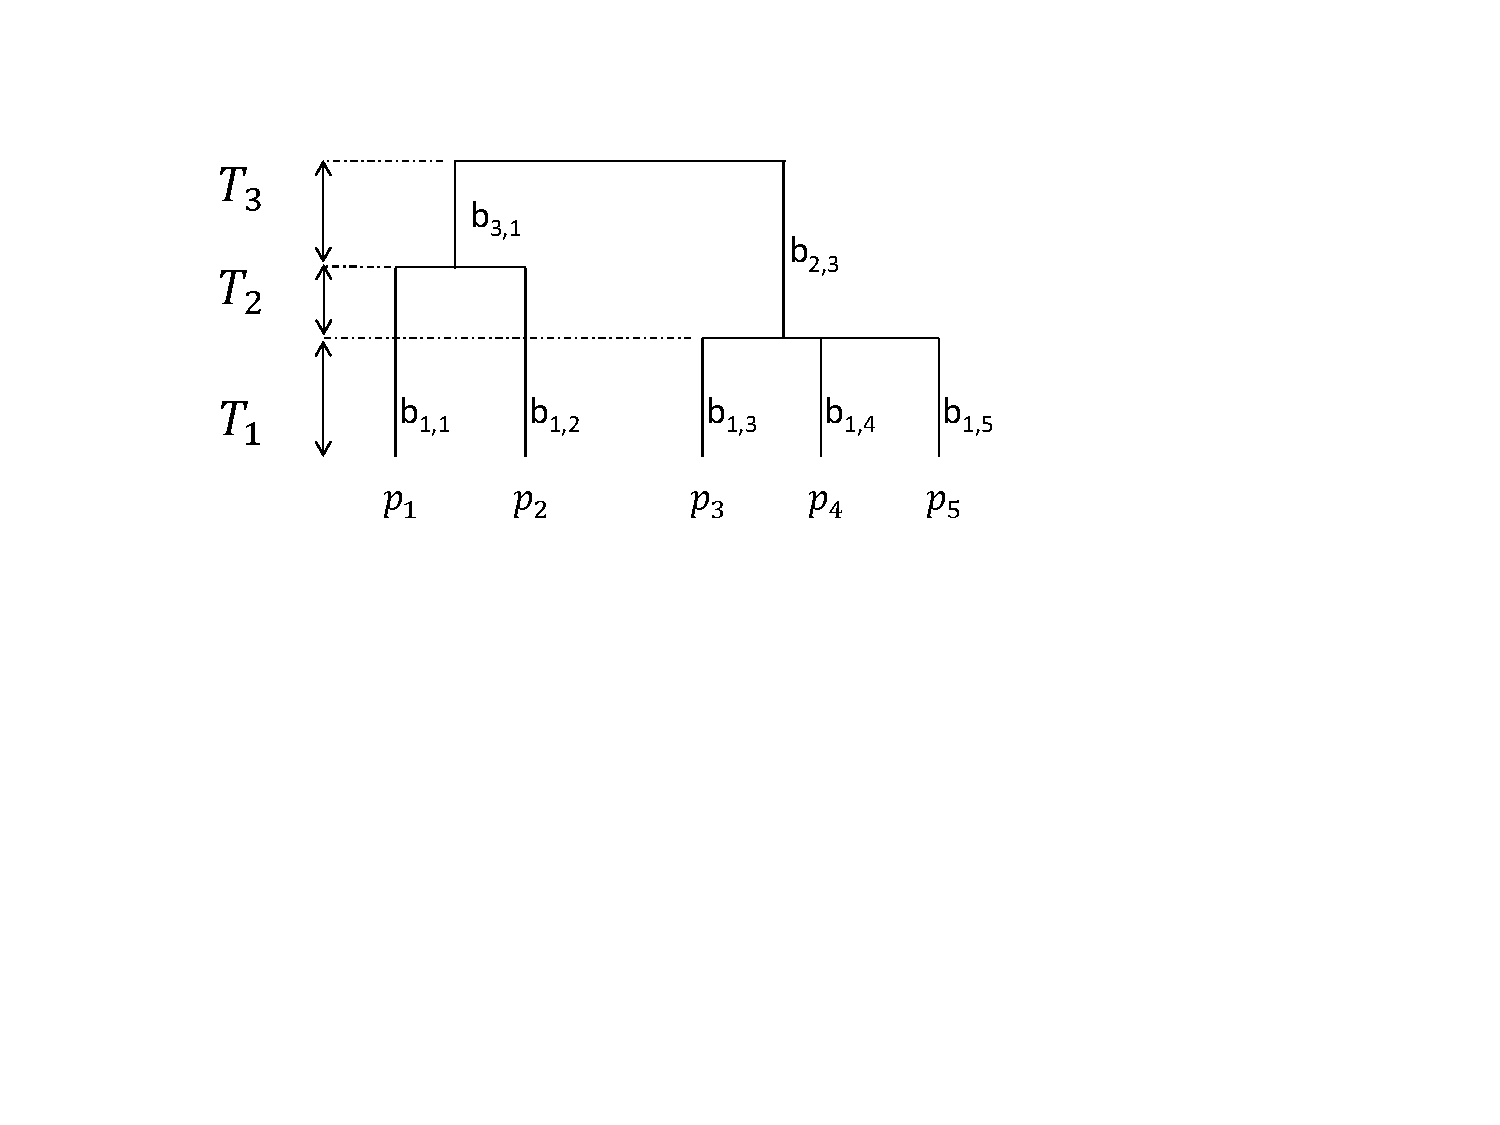
\includegraphics[width=0.8\linewidth]{images/ArbreA} 

}

\caption{Arbre phylogénétique ou fonctionnel hypothétique. L'arbre comprend 5 espèces dont les probabilités sont notées \(p_s\), 3 périodes de durées \(T_k\) délimitées par les noeuds. Les branches sont notées \(b\) et indicées par la période à laquelle elles se terminent et un numéro d'ordre.}\label{fig:ArbreA4}
\end{SCfigure}

\normalsize

La particularité évolutive \autocite{Isaac2007} (\emph{evolutive distinctiveness}, \(\mathit{ED}_s\)) de l'espèce \(s\) est la somme de la longueur des branches qui la relient à la racine de l'arbre, partagées entre tous les descendants de chaque branche.
Pour l'espèce 3 de la figure \ref{fig:ArbreA4}, \(\mathit{ED}_3\) est égal à \(l(b_{1,3})\), la longueur de la branche terminale propre à l'espèce 3, plus un tiers de la longueur de la branche qui relie la racine de l'arbre à la polytomie dont l'espèce 3 est issue.
Clairement, la diversité phylogénétique PD (section \ref{sec:PDFD}) est la somme des particularités évolutives de toutes les espèces de l'arbre.

\hypertarget{sec:OrigTax}{%
\subsection{Originalité taxonomique de Ricotta}\label{sec:OrigTax}}



\scriptsize

\begin{SCfigure}

{\centering 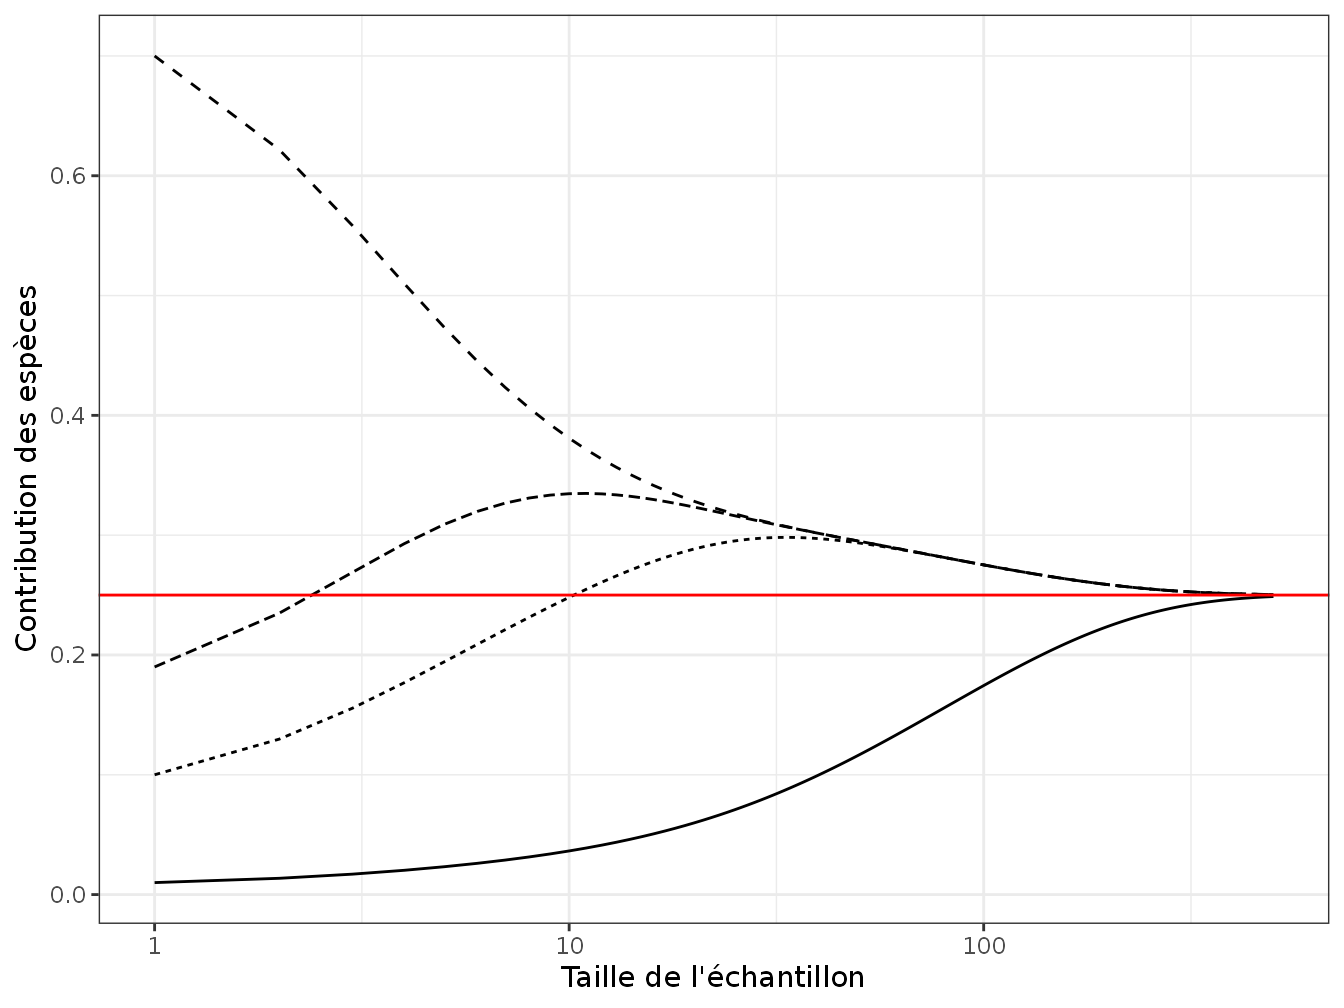
\includegraphics[width=0.8\linewidth]{MesuresBD_files/figure-latex/HurlbertCFig-1} 

}

\caption{Contribution des espèces à l'indice de Hurlbert. Les contributions de 4 espèces d'une communauté à l'indice sont représentées en fonction de la taille de l'échantillon \(n\). Les fréquences des espèces sont lisibles pour \(n = 1\): une espèce fréquente (probabilité égale à 0,7, supérieure à \(1/S\)), deux espèces peu fréquentes (0,19 et 0,1), et une espèce rare (0,01). Quand \(n\) est assez grand, toutes les contributions tendent vers \(1/S = 1/4\) (ligne horizontale).}\label{fig:HurlbertCFig}
\end{SCfigure}

\normalsize

\textcite{Ricotta2004a} construit un indice paramétrique (permettant de donner plus ou moins d'importance aux espèces rares) à partir de l'espérance du nombre d'espèces tirées dans un échantillon de taille \(n\) fixée (l'indice de \textcite{Hurlbert1971}):

\begin{equation}
  \label{eq:ESn}
  {\mathbb E}\left( S^n \right)
  = \sum_s{\left[ 1-\left( 1-p_s \right)^n  \right]}.
\end{equation}

Ricotta pondère cette espérance par l'originalité taxonomique de chaque espèce, notée \(w_s\) et normalise la mesure:
\begin{equation}
  \label{eq:Ricotta2004a}
  ^n{T}
  = \frac{\sum_s{w_s \left[ 1-\left( 1-p_s \right)^n  \right]}}{{\mathbb E}\left( S^n \right)}.
\end{equation}

L'originalité taxonomique est définie comme la distance phylogénétique moyenne entre l'espèce \(s\) et les autres: \(w_s={\sum_s{d_{s,t}}}/{(S-1)}\).

\textcite{Weikard2006} montrent que cette définition de \(w_s\) ne permet pas de satisfaire l'axiome de monotonicité d'ensemble.
La définition correcte de \(w_s=\sum_s{d_{s,t}}\), validée par \textcite{Ricotta2006}.

L'interprétation de \(^n{T}\) est plus intuitive en inversant la logique de sa construction.

\(w_s\) est l'originalité de l'espèce \(s\).
\({[1-(1-p_s)^n]}/{{\mathbb E}(S^n)}\) est la contribution de l'espèce \(s\) à l'espérance du nombre d'espèces, comprise entre 0 et 1.
\(^n{T}\) est donc l'originalité moyenne des espèces de la communauté, pondérée par la contribution de chaque espèce à l'espérance du nombre d'espèces observé, dans un échantillon de taille \(n\).
Cette contribution est présentée en figure \ref{fig:HurlbertCFig}.

Quand \(n=1\), c'est simplement la fréquence des espèces.
Quand \(n\) augmente, le poids des espèces fréquentes (dont la proabilité est supérieure à \(\frac{1}{S}\)) diminue alors que celui des espèces intermédiaires augmente.
Ce dernier atteint \({1}/{{\mathbb E}(S^n)}\) (une espèce est échantillonnée à coup sûr dès que l'échantillon est assez grand) d'autant plus rapidement que \(p_s\) est grand.
Il baisse ensuite alors que les espèces rares atteignent à leur tour progressivement leur poids maximal.

Quand \(n \to +\infty\), le numérateur tend vers FAD, et le dénominateur tend vers le nombre d'espèces: \(^n{T}\) tend vers MFAD.

Code R pour la figure \ref{fig:HurlbertCFig}:

\scriptsize

\begin{Shaded}
\begin{Highlighting}[]
\NormalTok{Ps <-}\StringTok{ }\KeywordTok{c}\NormalTok{(}\FloatTok{0.7}\NormalTok{, }\FloatTok{0.19}\NormalTok{, }\FloatTok{0.1}\NormalTok{, }\FloatTok{0.01}\NormalTok{)}
\NormalTok{S <-}\StringTok{ }\KeywordTok{length}\NormalTok{(Ps)}
\NormalTok{nRange <-}\StringTok{ }\DecValTok{1}\OperatorTok{:}\DecValTok{500}
\CommentTok{# Indice de Hurlbert}
\NormalTok{ESn <-}\StringTok{ }\KeywordTok{c}\NormalTok{(}\DecValTok{1}\NormalTok{, }\KeywordTok{sapply}\NormalTok{(nRange[}\OperatorTok{-}\DecValTok{1}\NormalTok{], }\ControlFlowTok{function}\NormalTok{(n) }\KeywordTok{Hurlbert}\NormalTok{(Ps, n)))}
\CommentTok{# Préparation du graphique}
\NormalTok{Xlab <-}\StringTok{ "Taille de l'échantillon"}
\NormalTok{Ylab <-}\StringTok{ "Contribution des espèces"}
\CommentTok{# Contribution de chaque espece à chaque valeur de n}
\NormalTok{Csn <-}\StringTok{ }\KeywordTok{sapply}\NormalTok{(}\DecValTok{1}\OperatorTok{:}\NormalTok{S, }\ControlFlowTok{function}\NormalTok{(s) }\KeywordTok{sapply}\NormalTok{(nRange, }
              \ControlFlowTok{function}\NormalTok{(n) (}\DecValTok{1}\OperatorTok{-}\NormalTok{(}\DecValTok{1}\OperatorTok{-}\NormalTok{Ps[s])}\OperatorTok{^}\NormalTok{n))}\OperatorTok{/}\NormalTok{ESn)}
\CommentTok{# Dataframe contenant les données}
\NormalTok{df <-}\StringTok{ }\KeywordTok{as.data.frame}\NormalTok{(}\KeywordTok{cbind}\NormalTok{(nRange, Csn))}
\KeywordTok{colnames}\NormalTok{(df) <-}\StringTok{ }\KeywordTok{c}\NormalTok{(}\StringTok{"n"}\NormalTok{, }\StringTok{"s07"}\NormalTok{, }\StringTok{"s019"}\NormalTok{, }\StringTok{"s01"}\NormalTok{, }\StringTok{"s001"}\NormalTok{)}
\CommentTok{# Graphique}
\NormalTok{ESnplot <-}\StringTok{ }\KeywordTok{ggplot}\NormalTok{(}\KeywordTok{gather}\NormalTok{(df, Sp, Contribution, }\OperatorTok{-}\NormalTok{n), }\KeywordTok{aes}\NormalTok{(}\DataTypeTok{x=}\NormalTok{n)) }\OperatorTok{+}
\StringTok{  }\KeywordTok{geom_line}\NormalTok{(}\KeywordTok{aes}\NormalTok{(}\DataTypeTok{y =}\NormalTok{ Contribution, }\DataTypeTok{lty=}\NormalTok{Sp)) }\OperatorTok{+}
\StringTok{  }\KeywordTok{geom_hline}\NormalTok{(}\DataTypeTok{yintercept=}\DecValTok{1}\OperatorTok{/}\DecValTok{4}\NormalTok{, }\DataTypeTok{col=}\StringTok{"red"}\NormalTok{) }\OperatorTok{+}
\StringTok{  }\KeywordTok{scale_x_log10}\NormalTok{() }\OperatorTok{+}
\StringTok{  }\KeywordTok{labs}\NormalTok{(}\DataTypeTok{x =}\NormalTok{ Xlab, }\DataTypeTok{y =}\NormalTok{ Ylab) }\OperatorTok{+}
\StringTok{  }\KeywordTok{theme}\NormalTok{(}\DataTypeTok{legend.position =} \StringTok{"none"}\NormalTok{)}
\NormalTok{ESnplot}
\end{Highlighting}
\end{Shaded}

\normalsize

\hypertarget{richesse-phyloguxe9nuxe9tique}{%
\subsection{Richesse phylogénétique}\label{richesse-phyloguxe9nuxe9tique}}

La particularité taxonomique moyenne \autocite{Warwick1995} (\emph{Average Taxonomic Distinctiveness, AvTD}) est la distance moyenne dans l'arbre entre deux espèces choisies au hasard.
C'est donc l'équivalent taxonomique de MFAD.
La variabilité phylogénétique des espèces \autocite{Helmus2007} (\emph{Phylogenetic Species Variability, PSV}) est la même mesure, obtenue à partir du modèle d'évolution suivant un mouvement brownien \autocite{Felsenstein1985}.
La distance moyenne entre deux espèces est dans ce cadre proportionnelle à la covariance de leurs traits fonctionnels.
La richesse phylogénétique des espèces, PSR, est PSV multipliée par le nombre d'espèces: c'est l'équivalent taxonomique de FAD.

La diversité FD de Faith (section \ref{sec:PDFD}), égale à la somme des longueurs des branches de l'arbre, semble avoir fait consensus, d'où un moindre développement des mesures de richesse que dans la littérature fonctionnelle.

\hypertarget{indices-de-cadotte}{%
\subsection{Indices de Cadotte}\label{indices-de-cadotte}}

\textcite{Cadotte2010} proposent un ensemble de mesure phylogénétiques: équitabilité, déséquilibre d'abondance et diversité de la particularité evolutive.

\hypertarget{equitabilituxe9-phyloguxe9nuxe9tique}{%
\subsubsection{Equitabilité phylogénétique}\label{equitabilituxe9-phyloguxe9nuxe9tique}}

Les branches terminales de l'arbre phylogénétique sont ici à la base de la définition de l'équitabilité.
figure \ref{fig:ArbreA3}, les branches \(b_{1,s}\) sont les segments terminés par une feuille (au bas de l'arbre), c'est-à-dire que leur longueur est la partie de l'arbre que les espèces ne partagent pas.
La mesure d'équitabilité est
\begin{equation}
  \mathit{PAE} = \frac{\mathit{PD} + \sum_s{l(b_{1,s})(n_s-1)}}{\mathit{PD} + (\frac{n}{S}-1)\sum_s{l(b_{1,s})} }.
\end{equation}

\scriptsize

\begin{SCfigure}

{\centering 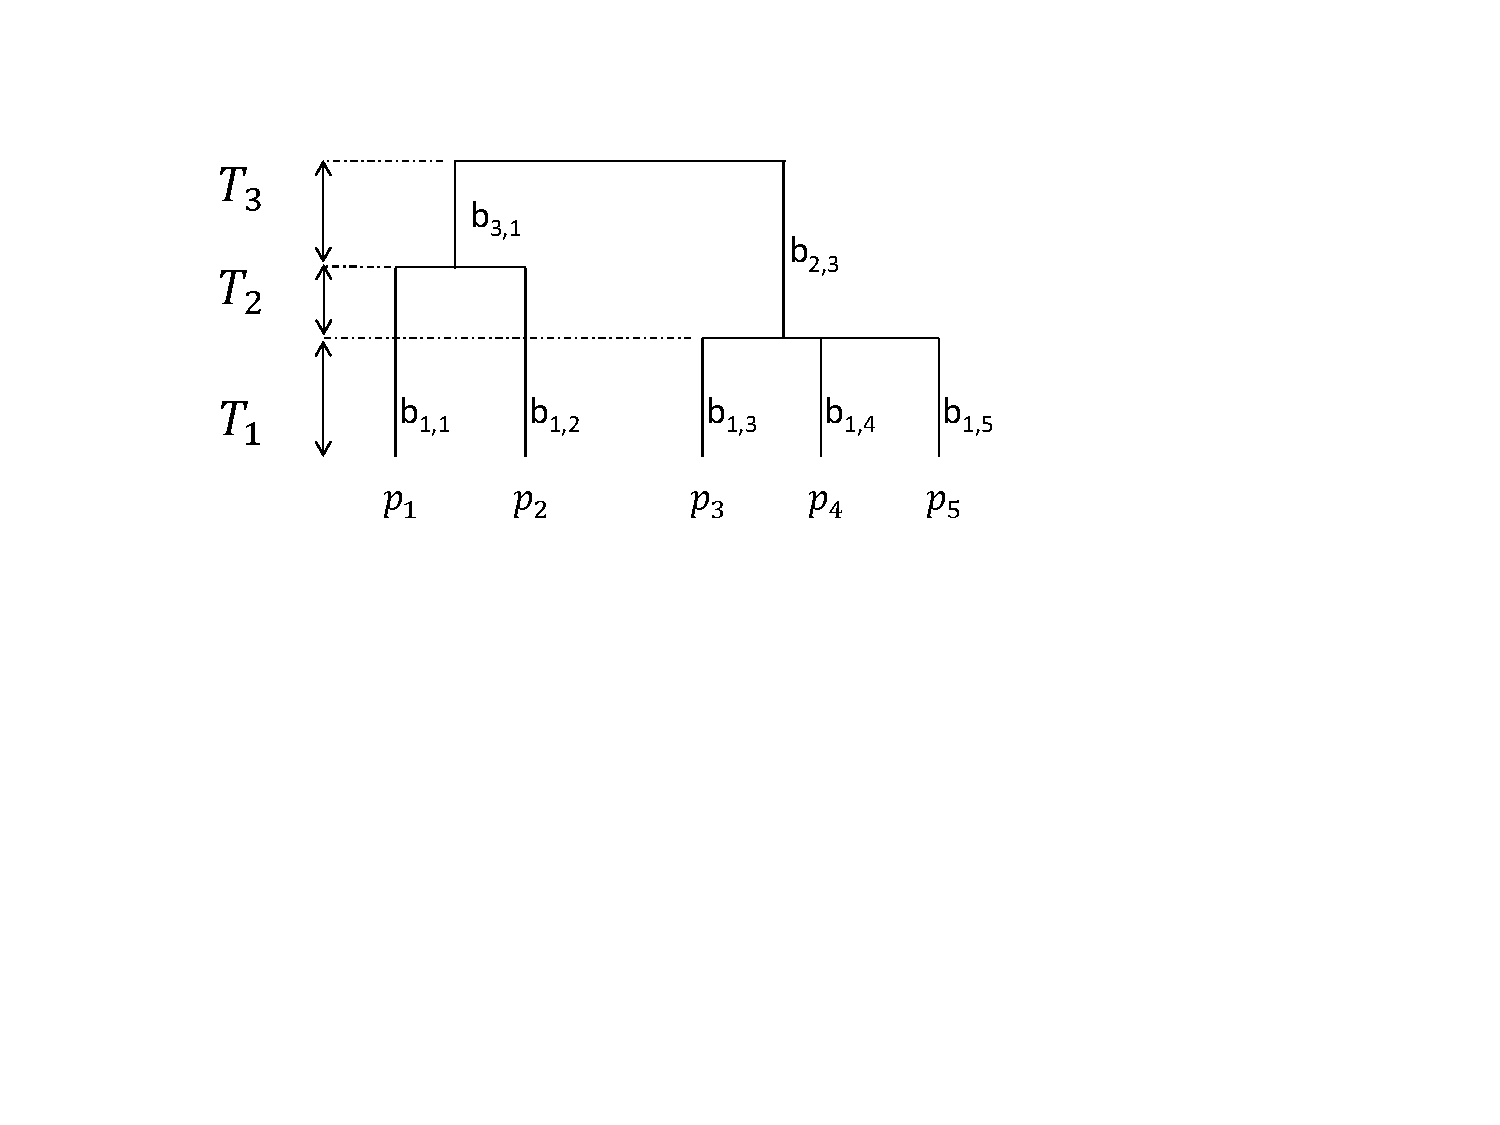
\includegraphics[width=0.8\linewidth]{images/ArbreA} 

}

\caption{Arbre phylogénétique ou fonctionnel hypothétique.}\label{fig:ArbreA3}
\end{SCfigure}

\normalsize

\(\mathit{PAE}\) vaut 1 quand les espèces sont sont distribuées équitablement pour la longueur des branches.
Une valeur plus grande est obtenue quand les espèces sont concentrées au bout des longues branches, et inversement si \(0<\mathit{PAE}<1\).

\hypertarget{duxe9suxe9quilibre-dabondance}{%
\subsubsection{Déséquilibre d'abondance}\label{duxe9suxe9quilibre-dabondance}}

L'équilibre d'abondance est défini par une distribution aléatoire des espèces par division de l'effectif total à partir de la racine de l'arbre phylogénétique.
En figure \ref{fig:ArbreA3}, en partant de la racine, la moitié des individus est supposée se répartir sur chaque branche.
À la période 2, les effectifs de la branche de gauche se partagent en deux parties égales.
À partir du nombre total d'individus de la communauté, \(n\), le nombre attendu d'individus \(n_s^0\) de l'espèce \(s\) est une fraction de \(n\) correspondant au nombre de noeuds et au nombre de branches partant de chaque noeud.
On note \(y_{k,s}\) le nombre de branches partant du noeud ancestral de l'espèce \(s\) à la période \(k\), s'il existe, \(y_{k,s}=1\) sinon:
\begin{equation}
  n_s^0 = \frac{n}{\prod_{k=2}^{K}{y_{k,s}}}.
\end{equation}

En figure \ref{fig:ArbreA3}, pour l'espèce 3, \(y_{1,3}=3\) (l'espèce est issue d'une polytomie), \(y_{2,3}=1\) (absence de noeud) et \(y_{3,3}=2\) (la racine de l'arbre est dichotomique).
On s'attend donc à ce que l'espèce 3 soit représentée par un sixième des individus.

L'indice de déséquilibre d'abondance mesure l'écart à cette distribution théorique:
\begin{equation}
  \label{eq:IAC}
  \mathit{IAC} = \frac{\sum_s{|n_s - n_s^0|}}{\nu}.
\end{equation}

\(\nu\) est le nombre de noeuds de l'arbre (3 dans l'exemple de la figure \ref{fig:ArbreA3}).

\hypertarget{diversituxe9-de-la-particularituxe9-uxe9volutive}{%
\subsubsection{Diversité de la particularité évolutive}\label{diversituxe9-de-la-particularituxe9-uxe9volutive}}

L'entropie de Shannon peut être appliquée pour mesurer la diversité des particularités évolutives:
\begin{equation}
  \label{eq:HED}
  H_{\mathit{ED}} = -\sum_s{\frac{\mathit{ED}_s}{\mathit{PD}} \ln\frac{\mathit{ED}_s}{\mathit{PD}}}.
\end{equation}

L'équitabilité des particularités évolutives est celle de Pielou:

\begin{equation}
  \label{eq:EED}
  E_{\mathit{ED}} = \frac{H_{\mathit{ED}}}{\ln{S}}.
\end{equation}

Ces mesures ne prennent pas en compte les abondances des espèces.
Pour y remédier, il suffit d'ajouter une période de durée nulle à chaque feuille de l'arbre, correspondant à une polytomie entre les \(n_s\) individus de chaque espèce.
La particularité évolutive \(\mathit{AED}_s\) des individus de l'espèce \(s\), est calculée en partageant la longueur de chaque branche ancestrale entre le nombre d'individus qui en descendent (et non le nombre d'espèces).
Alors \(\mathit{PD} = \sum_s{n_s \mathit{AED}_s}\).
L'entropie devient
\begin{equation}
  \label{eq:HAED}
  H_{\mathit{AED}} = -\sum_s{\frac{n_s \mathit{AED}_s}{\mathit{PD}} \ln\frac{n_s \mathit{AED}_s}{\mathit{PD}}}
\end{equation}
et l'équitabilité correspondante est
\begin{equation}
  \label{eq:EAED}
  E_{\mathit{AED}} = \frac{H_{\mathit{AED}}}{\ln{N}}.
\end{equation}

Ces indices ne mesurent pas la diversité phylogénétique au sens des autres mesures présentées dans ce chapitre.
Ils mesurent la diversité de le particularité évolutive, autrement dit du temps d'évolution accumulé par chaque espèce ou chaque individu.
Pour un nombre d'espèces fixé, \(E_{\mathit{ED}}\) atteint son maximum quand les valeurs de \(\mathit{ED}_s\) sont toutes identiques.
Un arbre phylogénétique composé d'une seule branche depuis la racine terminé par une polytomie de longueur nulle portant toutes les espèces correspond à cette description.
Dans cet exemple, les espèces ont une divergence évolutive nulle, mais \(E_{\mathit{ED}} = S\), son maximum possible.

\hypertarget{diversituxe9-de-scheiner}{%
\section{Diversité de Scheiner}\label{diversituxe9-de-scheiner}}

\textcite{Scheiner2012} développe un cadre unifié pour mesurer la diversité spécifique, phylogénétique ou fonctionnelle, séparément ou simultanément.
L'idée générale est que toute quantité partagée par les espèces (le nombre d'individus, le temps d'évolution accumulé, la taille des niches écologique) peut être traduite en nombre de Hill.

La diversité spécifique est simplement \(^{q}\!D\). Scheiner la note \(^{q}\!D(A)\), pour diversité d'abondance.

La diversité phylogénétique \(^{q}\!D(P)\) ne prend pas en compte les abondances mais mesure la diversité de la divergence évolutive des espèces.
La divergence totale dans un arbre phylogénétique (pas forcément ultramétrique) est la longueur totale des branches (c'est-à-dire FD).
Elle est répartie entre toutes les espèces: la longueur de chaque branche (représentant une quantité d'évolution) est partagée à parts égales entre les espèces qui en descendent.
La divergence de l'espèce 1 de la figure \ref{fig:Arbre} est \(T1+T2\), la longueur de la branche terminale, plus \({T3}/{2}\), parce que la branche est partagée par les espèces 1 et 2.
La divergence de l'espèce 1, est donc \(L_1 = T1+T2+{T3}/{2}\).
La part de la divergence de l'espèce \(s\) est \(l_s = {L_s}/{FD}\).
La diversité phylogénétique est le nombre de Hill des divergences:

\begin{equation}
  \label{eq:HillDivergences}
  ^{q}\!D = {\left(\sum^S_{s=1}{l_s^q}\right)}^{\frac{1}{1-q}}.
\end{equation}

La diversité fonctionnelle \(^{q}\!D(F)\) est la diversité des tailles des niches. La taille de la niche est définie par Scheiner comme le volume de l'hypersphère (dans l'espace des traits fonctionnels de dimension \(m\)) centrée sur chaque espèce dont le rayon est la moitié de la distance à l'espèce la plus proche pour que les sphères ne se superposent pas.
Une meilleure définition \autocite{Presley2014} de la taille de la niche est la somme des distances aux autres espèces: \(t_s = \sum_t{d_{s,t}}\). La part de chaque espèce est \(f_s={t_s}/{\sum_t{t_t}}\) et la définition de la diversité fonctionnelle est

\begin{equation}
  \label{eq:DqT}
  ^{q}\!D(T) = {\left(\sum^S_{s=1}{f_s^q}\right)}^{\frac{1}{1-q}}.
\end{equation}

La diversité peut prendre en compte plusieurs composantes, pas exemple l'abondance et la phylogénie pour définir

\begin{equation}
  \label{eq:qDAP}
  ^{q}\!D(AP) = {\left(\sum^S_{s=1}{\left(\frac{n_s L_s}{\sum^S_{t=1}{n_t L_t}}\right)^q}\right)}^{\frac{1}{1-q}}.
\end{equation}

La diversité d'abondance et phylogénétique est la diversité des divergences pondérées par les effectifs des espèces.
La mesure de biodiversité de Scheiner, incluant les trois composantes, est

\begin{equation}
  \label{eq:qDAF}
  ^{q}\!D(APF) = {\left(\sum^S_{s=1}{\left(\frac{n_s L_s t_s}{\sum^S_{t=1}{n_t L_t t_t}}\right)^q}\right)}^{\frac{1}{1-q}}.
\end{equation}

Son interprétation est moins immédiate.
Chaque espèce est associée à une fraction d'une des trois dimensions de la diversité (abondance, temps d'évolution cumulé, taille des niches).
Elle occupe un parallélépipède de dimensions \((p_s, l_s, f_s)\) dans le cube de dimension 1 qui les contient toutes.
Cette représentation ne donne pas d'importance particulière à l'abondance, et peut être appliquée à un nombre quelconque de dimensions.
La mesure de biodiversité est la diversité des volumes occupés par les espèces, normalisés par leur somme (qui n'est pas égale à 1).

En se limitant à deux dimensions pour la lisibilité, la figure \ref{fig:ScheinerPsfsFig} présente les rectangles correspondant à la diversité d'abondance et fonctionnelle occupés par les espèces de la méta-communauté \texttt{Paracou618}, classées par fréquences décroissantes.



\scriptsize

\begin{SCfigure}

{\centering 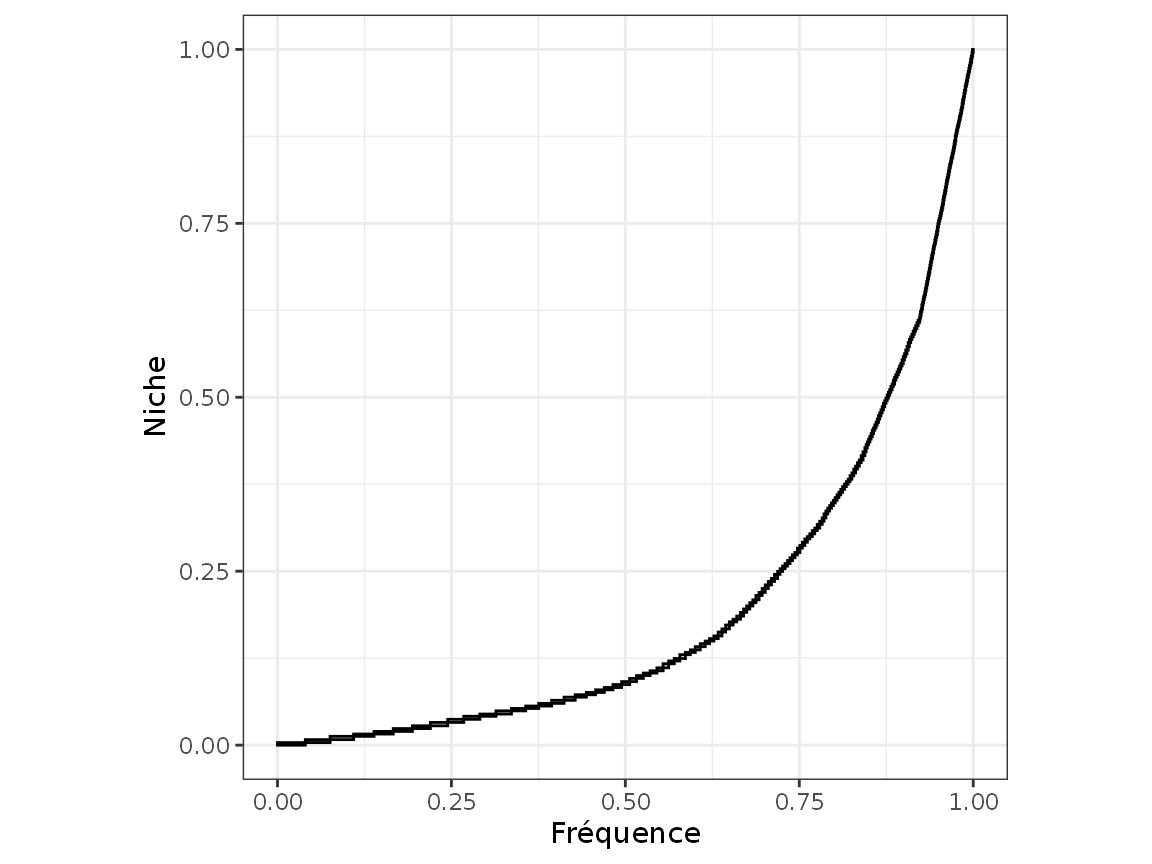
\includegraphics[width=0.8\linewidth]{MesuresBD_files/figure-latex/ScheinerPsfsFig-1} 

}

\caption{Rectangles de surface fréquence \(\times\) taille de niche des espèces de la méta-communauté \texttt{Paracou618}. La diversité de Scheiner \(^{q}\!D(AF)\) est la diversité de leur surface.}\label{fig:ScheinerPsfsFig}
\end{SCfigure}

\normalsize

Code R:

\scriptsize

\begin{Shaded}
\begin{Highlighting}[]
\CommentTok{# Probabilités}
\NormalTok{Ps <-}\StringTok{ }\NormalTok{Paracou618.MC}\OperatorTok{$}\NormalTok{Ps[Paracou618.MC}\OperatorTok{$}\NormalTok{Ps}\OperatorTok{>}\DecValTok{0}\NormalTok{]}
\NormalTok{Ps <-}\StringTok{ }\KeywordTok{sort}\NormalTok{(Ps, }\DataTypeTok{decreasing =} \OtherTok{TRUE}\NormalTok{)}
\CommentTok{# Fréquences cumulées}
\NormalTok{PsCum <-}\StringTok{ }\KeywordTok{cumsum}\NormalTok{(Ps)}
\NormalTok{Xgauche <-}\StringTok{ }\KeywordTok{c}\NormalTok{(}\DecValTok{0}\NormalTok{, PsCum)}
\NormalTok{Xdroite <-}\StringTok{ }\KeywordTok{c}\NormalTok{(PsCum, }\DecValTok{1}\NormalTok{)}
\CommentTok{# Matrice de distances fonctionnelles}
\NormalTok{DistanceMatrix <-}\StringTok{ }\KeywordTok{as.matrix}\NormalTok{(Paracou618.dist)}
\CommentTok{# Mise en correspondance de la matrice et du vecteur de probabilités}
\NormalTok{DistanceMatrix <-}\StringTok{ }\NormalTok{DistanceMatrix[}\KeywordTok{names}\NormalTok{(Ps), }\KeywordTok{names}\NormalTok{(Ps)]}
\CommentTok{# Taille des niches}
\NormalTok{ts <-}\StringTok{ }\KeywordTok{rowSums}\NormalTok{(DistanceMatrix)}
\NormalTok{fs <-}\StringTok{ }\NormalTok{ts}\OperatorTok{/}\KeywordTok{sum}\NormalTok{(ts)}
\CommentTok{# Fréquences cumulées}
\NormalTok{fsCum <-}\StringTok{ }\KeywordTok{cumsum}\NormalTok{(fs)}
\NormalTok{Ybas <-}\StringTok{ }\KeywordTok{c}\NormalTok{(}\DecValTok{0}\NormalTok{, fsCum)}
\NormalTok{Yhaut <-}\StringTok{ }\KeywordTok{c}\NormalTok{(fsCum, }\DecValTok{1}\NormalTok{)}
\CommentTok{# Rectangles occupés par chaque espèce}
\KeywordTok{ggplot}\NormalTok{(}\KeywordTok{data.frame}\NormalTok{(Xgauche, Ybas, Xdroite, Yhaut)) }\OperatorTok{+}
\StringTok{  }\KeywordTok{geom_rect}\NormalTok{(}\KeywordTok{aes}\NormalTok{(}\DataTypeTok{xmin=}\NormalTok{ Xgauche, }\DataTypeTok{xmax=}\NormalTok{ Xdroite, }\DataTypeTok{ymin=}\NormalTok{ Ybas, }\DataTypeTok{ymax=}\NormalTok{ Yhaut), }
             \DataTypeTok{color =} \StringTok{"black"}\NormalTok{, }\DataTypeTok{fill =} \StringTok{"white"}\NormalTok{) }\OperatorTok{+}
\StringTok{  }\KeywordTok{coord_fixed}\NormalTok{() }\OperatorTok{+}
\StringTok{  }\KeywordTok{labs}\NormalTok{(}\DataTypeTok{x =} \StringTok{"Fréquence"}\NormalTok{, }\DataTypeTok{y=}\StringTok{"Niche"}\NormalTok{)}
\end{Highlighting}
\end{Shaded}

\normalsize

La diversité d'abondance et fonctionnelle est la diversité de la surface des rectangles:

\scriptsize

\begin{Shaded}
\begin{Highlighting}[]
\NormalTok{Surface <-}\StringTok{ }\NormalTok{Ps }\OperatorTok{*}\StringTok{ }\NormalTok{fs}
\NormalTok{Rs <-}\StringTok{ }\NormalTok{Surface}\OperatorTok{/}\KeywordTok{sum}\NormalTok{(Surface)}
\KeywordTok{Diversity}\NormalTok{(Rs, }\DataTypeTok{q =} \DecValTok{2}\NormalTok{)}
\end{Highlighting}
\end{Shaded}

\begin{verbatim}
##     None 
## 71.72482
\end{verbatim}

\normalsize

Le profil de diversité d'abondance et fonctionnelle est en figure \ref{fig:ProfilDqAFFig}.



\scriptsize

\begin{SCfigure}

{\centering 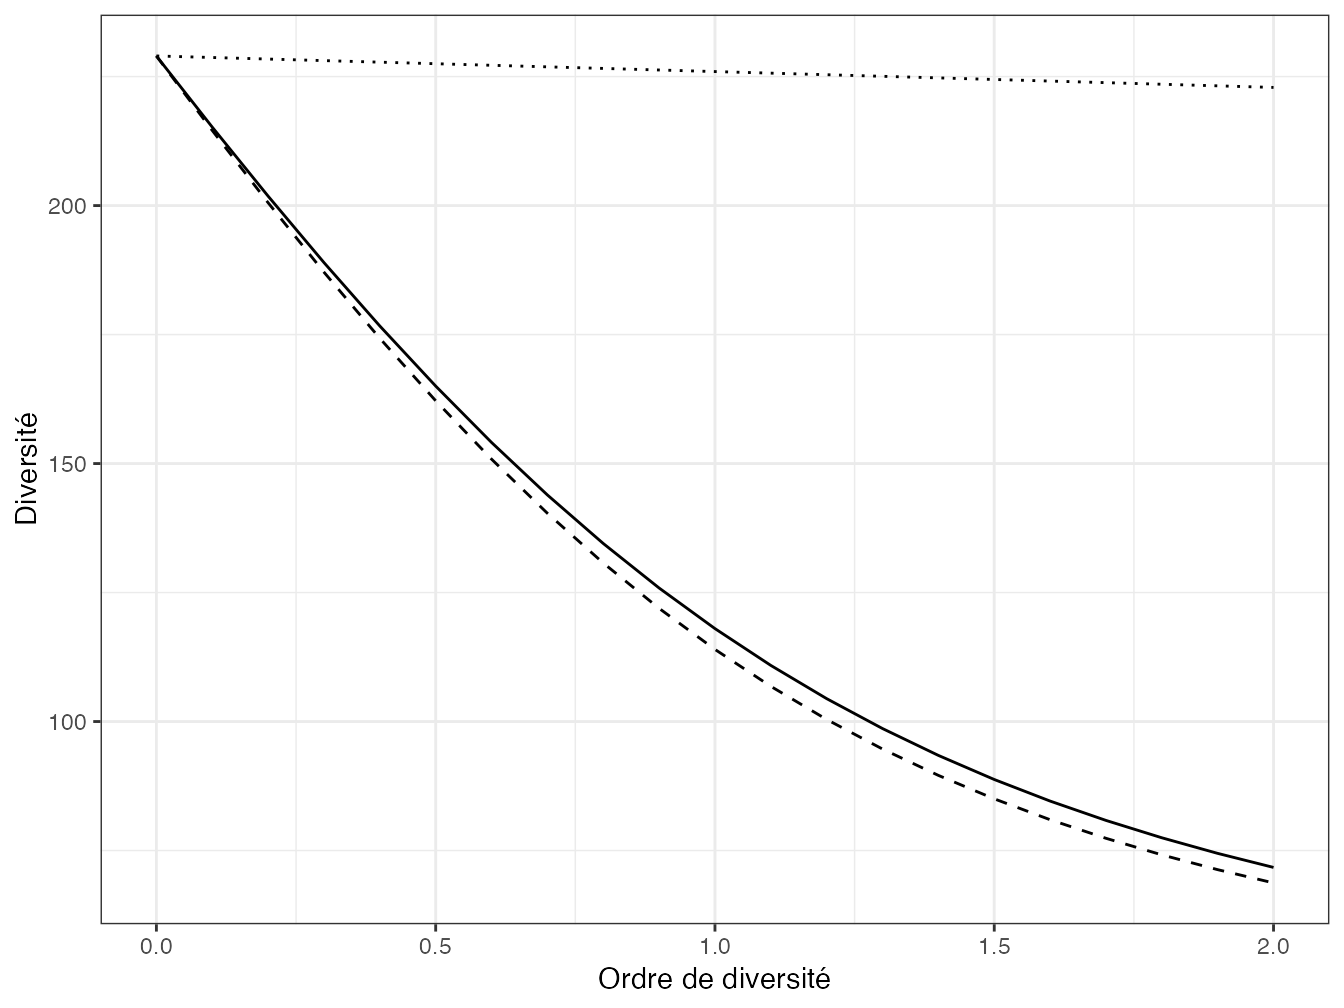
\includegraphics[width=0.8\linewidth]{MesuresBD_files/figure-latex/ProfilDqAFFig-1} 

}

\caption{Profil de diversité d'abondance et fonctionnelle de Scheiner de la méta-communauté \texttt{Paracou618}. Pointillés longs: diversité d'abondance; pointillés courts: diversité fonctionnelle; trait plein: diversité d'abondance et fonctionnelle.}\label{fig:ProfilDqAFFig}
\end{SCfigure}

\normalsize

Code R:

\scriptsize

\begin{Shaded}
\begin{Highlighting}[]
\KeywordTok{autoplot}\NormalTok{(}\KeywordTok{CommunityProfile}\NormalTok{(Diversity, Rs), }
         \DataTypeTok{xlab=}\StringTok{"Ordre de diversité"}\NormalTok{, }\DataTypeTok{ylab=}\StringTok{"Diversité"}\NormalTok{) }\OperatorTok{+}
\KeywordTok{geom_line}\NormalTok{(}\DataTypeTok{data =} \KeywordTok{as.data.frame.list}\NormalTok{(}\KeywordTok{CommunityProfile}\NormalTok{(Diversity, Ps)), }
          \DataTypeTok{mapping =} \KeywordTok{aes}\NormalTok{(x, y), }\DataTypeTok{lty =} \DecValTok{2}\NormalTok{) }\OperatorTok{+}
\KeywordTok{geom_line}\NormalTok{(}\DataTypeTok{data =} \KeywordTok{as.data.frame.list}\NormalTok{(}\KeywordTok{CommunityProfile}\NormalTok{(Diversity, fs)),}
          \DataTypeTok{mapping =} \KeywordTok{aes}\NormalTok{(x, y), }\DataTypeTok{lty=}\DecValTok{3}\NormalTok{)}
\end{Highlighting}
\end{Shaded}

\normalsize

La notion de diversité phylogénétique ou fonctionnelle traitée par Scheiner est assez différente de celles vues précédemment parce qu'elle considère toutes les dimensions de façon symétrique: l'ordre de diversité, \(q\), s'applique à toutes les dimensions.
Si \(q\) est grand, les espèces dont le produit des dimensions de la diversité est petit (que l'espèce soit rare, ait une divergence phylogénétique faible ou une niche étroite) sont négligées, alors que \(q\) n'affecte que la fréquence dans le cadre de la phylodiversité \(^{q}\!\bar{D}\) ou la banalité pour \(^q\!D^{\mathbf{Z}}\).

\hypertarget{diversituxe9-de-solow-et-polasky}{%
\section{Diversité de Solow et Polasky}\label{diversituxe9-de-solow-et-polasky}}

\textcite{Solow1994} relient la richesse fonctionnelle ou phylogénétique à la probabilité de trouver au moins une espèce intéressante (par exemple, capable de fournir une molécule utile) dans une communauté.

Les distances entre espèces sont supposées connues, qu'elles soient fonctionnelle, phylogénétique ou autre.
La probabilité qu'une espèce quelconque soit intéressante est fixée à \(p\), par exemple à partir de l'expérience passée (si une espèce criblée sur 100 fournit une molécule utile, \(p=1\%\)).
En absence d'information sur les espèces, \(p\) est \emph{a priori} identique pour toutes mais on suppose une corrélation entre les probabilités dépendant de la distance entre les espèces.
Formellement, une fonction de similarité entre les espèces \(s\) et \(t\) est définie: \(z_{s,t}=f(d_{s,t})\).
Cette fonction est décroissante entre 1 (quand la distance est nulle) et 0 (à distance infinie); par exemple \(f(d_{s,t}) = e^{-u d_{s,t}}\) où \(u\) est une constante strictement positive.
La matrice \(\mathbf{Z}\) réunit les éléments \(z_{s,t}\).

On définit ensuite la variable de Bernoulli \(B_s\) (d'espérance \(p_s\)) qui vaut 1 si l'espèce \(s\) est intéressante.
\(z_{s,t}\) est, par construction du modèle, la corrélation entre \(B_s\) et \(B_t\): deux espèces très proches ont la même probabilité d'être intéressante, deux espèces très éloignées ont des probabilités indépendantes.
La probabilité qu'au moins une espèce soit intéressante est minorée par \(p^2 \mathbf{1}_S' \mathbf{Z}^{-1} \mathbf{1}_S\), où \(\mathbf{1}_S\) est le vecteur de longueur \(S\) ne contenant que des 1, \('\) indique la transposée et \(\mathbf{Z}^{-1}\) est la matrice inverse de \(\mathbf{Z}\) (son existence est garantie puisque \(\mathbf{Z}\) est une matrice de variance-covariance).
La valeur de \(p\) est incertaine et sans grand intérêt.

\(V = \mathbf{1}_S' \mathbf{Z}^{-1} \mathbf{1}_S\) est la mesure de diversité de Solow et Polasky.
Elle rend compte de la dispersion des espèces: moins les espèces sont similaires, plus la probabilité que l'une d'elle au moins soit intéressante est élevée, conditionnellement au nombre d'espèces et à \(p\).
Si les espèces sont infiniment éloignées les unes des autres, \(\mathbf{Z}\) est la matrice identité et la diversité est égale à la richesse: \(V\) est donc un nombre effectif d'espèces, c'est-à-dire le nombre d'espèces totalement dissimilaires nécessaires pour obtenir la diversité observée.
À l'opposé, si toutes les espèces sont identiques, \(\mathbf{Z}\) ne contient que des 1 et la diversité vaut 1.

\hypertarget{sec:PDFD}{%
\section{FD et PD}\label{sec:PDFD}}



\scriptsize

\begin{SCfigure}

{\centering 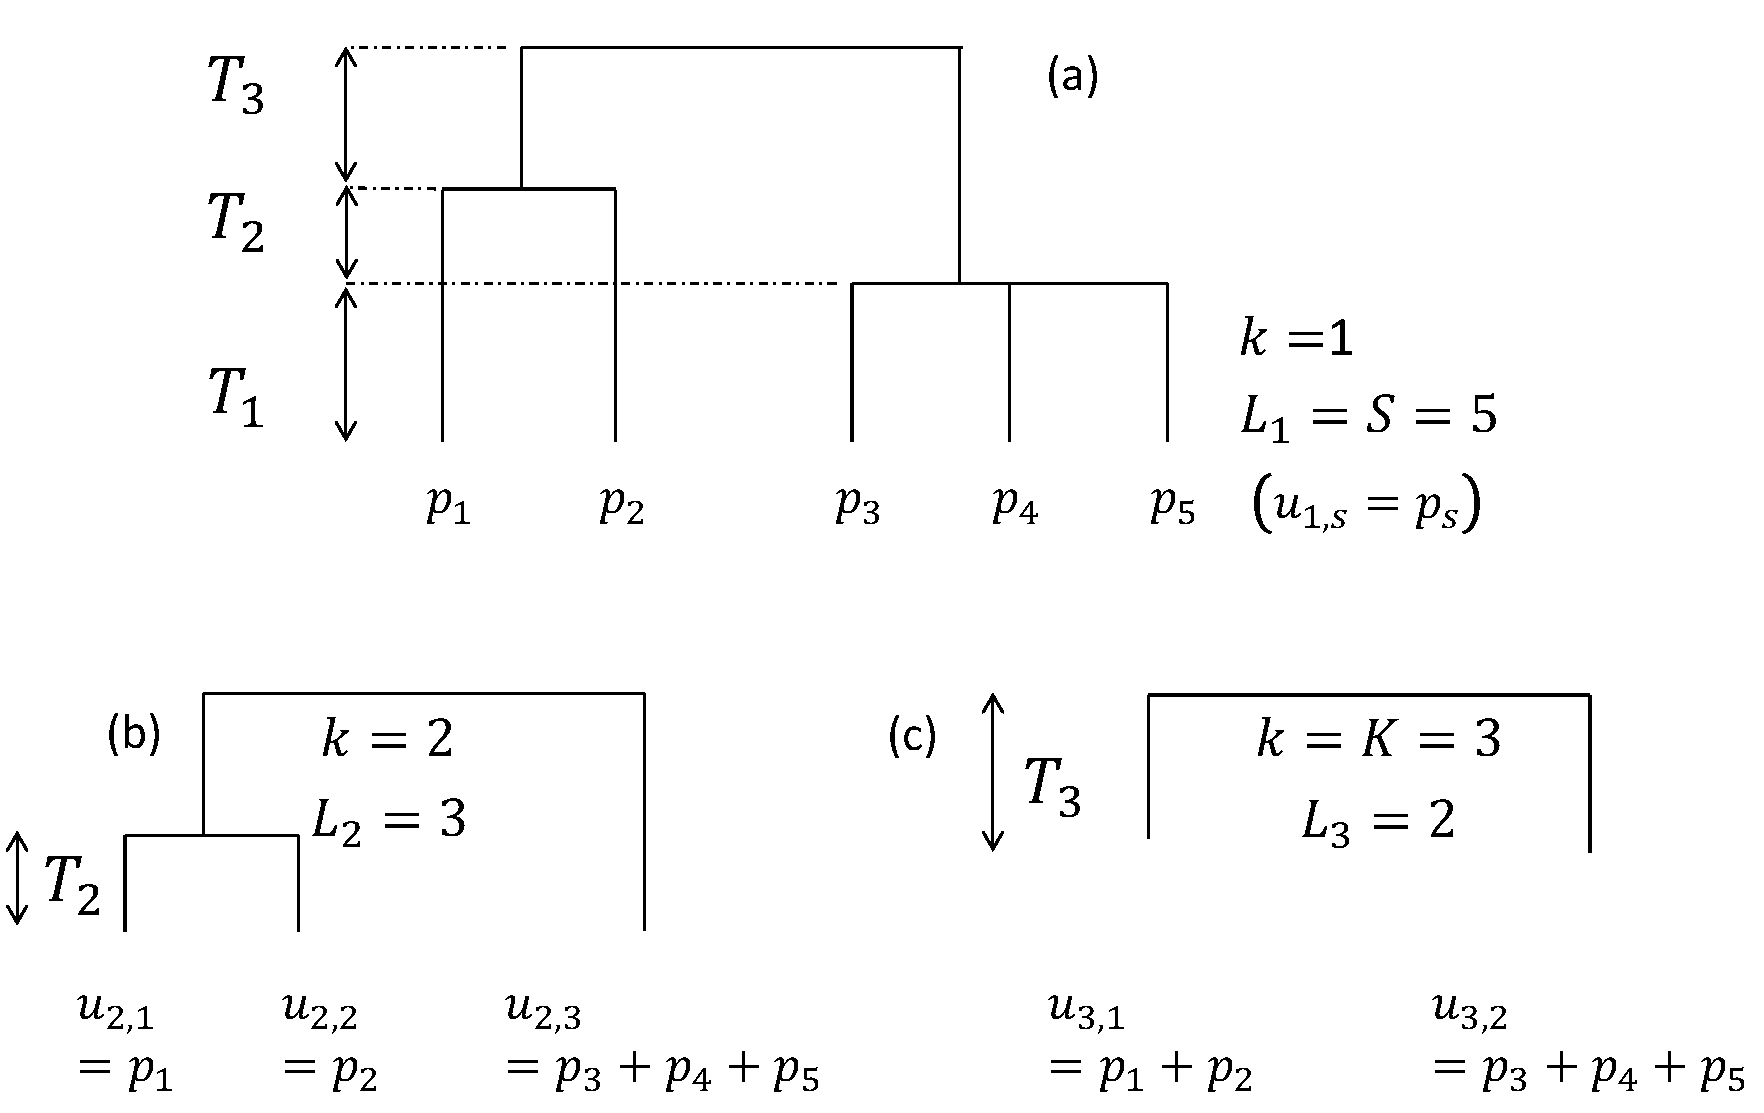
\includegraphics[width=0.8\linewidth]{images/Arbre} 

}

\caption{Arbre phylogénétique ou fonctionnel hypothétique. (a) Arbre complet. 5 espèces sont présentes (\(S = 5\)). Une période de l'arbre est définie entre deux noeuds successifs: l'arbre contient \(K = 3\) périodes. Les hauteurs des périodes sont notées \(T_k\). À chaque période correspond un arbre plus simple: (b) pour la période 2, (c) pour la période 3 dans lequel les espèces originales sont regroupées. Le nombre de feuilles de ces arbres est noté \(L_k\). Les probabilités pour un individu d'appartenir à une feuille sont notées \(u_{k,l}\).}\label{fig:Arbre}
\end{SCfigure}

\normalsize

Si la dissimilarité entre les espèces est représentée par un dendrogramme, les indices de diversité les plus simples sont la diversité phylogénétique \autocite{Faith1992} et sa transposition, la diversité fonctionnelle \autocite{Petchey2002}.

Étant donné un arbre contenant toutes les espèces ou tous les individus étudiés, PD ou FD sont égaux à la somme de la longueur des branches (figure \ref{fig:Arbre}: \(\mathit{PD}=5\times T_1 + 3\times T_2 + 2\times T_3)\).
Si les noeuds de l'arbre phylogénétique sont datés, PD peut être considéré comme une accumulation de temps d'évolution par la communauté étudiée: \textcite{Sol2017} montrent par exemple que les milieux urbanisés ont un déficit de 450 millions d'années d'évolution dans les communautés d'oiseaux relativement aux environnements naturels voisins.

Dans le cas particulier ou toutes les branches sont de longueur 1, c'est-à-dire que toutes les espèces sont liées à la même racine (on dira que l'arbre est parfaitement régulier), PD et FD sont égales à la richesse spécifique.

Le package \emph{entropart} fournit la fonction \texttt{PDFD}:

\scriptsize

\begin{Shaded}
\begin{Highlighting}[]
\CommentTok{# Vecteur des probabilités}
\NormalTok{Ps <-}\StringTok{ }\NormalTok{Paracou618.MC}\OperatorTok{$}\NormalTok{Ps}
\KeywordTok{PDFD}\NormalTok{(Ps, Paracou618.Taxonomy)}
\end{Highlighting}
\end{Shaded}

\begin{verbatim}
## None 
##  395
\end{verbatim}

\normalsize

\textcite{Chao2014b} fournissent un estimateur de PD (ou FD) permettant de l'estimer sans biais pour un échantillon plus petit que celui observé et de façon fiable pour un échantillon de taille double au maximum. Ces estimateurs permettent de tracer des courbes de raréfaction et d'extrapolation.

En même temps que Faith, \textcite{Weitzman1992} a établi une fonction de diversité identique à PD.
À partir d'une matrice de dissimilarités entre espèces, un arbre est construit par la méthode suivante.
Les deux espèces les plus proches sont rassemblées.
L'une d'elles, celle qui diminue le moins la longueur totale des branches de l'arbre final en la retirant, est l'espèce de \emph{lien}, l'autre est l'espèce \emph{représentative} du clade.
L'espèce de lien est retirée et le regroupement poursuivi entre les deux nouvelles espèces les plus proches.
À chaque étape, l'espèce de lien est retirée jusqu'au regroupement final entre les deux dernières espèces.
La difficulté est que l'arbre final n'est pas connu aux premiers stades de regroupement donc tous les arbres doivent être testés pour trouver la solution unique.
La diversité est la somme des distances entre les espèces de lien et leur espèce représentative, c'est-à-dire la longueur totale des branches de l'arbre obtenu.
L'application à la conservation est que les espèces représentatives doivent être favorisées par rapport aux espèces de lien; en d'autres termes, les espèces dont les branches sont les plus courtes dans l'arbre sont celles qui apportent le moins de diversité.
Ce résultat est assez évident quand on dispose d'un arbre phylogénétique.
L'originalité de la méthode de Weitzman est de fournir un algorithme pour créer l'arbre à partir d'une matrice de distances qui est cohérent avec la mesure de diversité appliquée.

La mesure de diversité peut être combinée avec une probabilité d'extinction de chaque espèce (à dire d'expert) pour calculer l'espérance de la diversité à une échéance donnée \autocite{Weitzman1993}: \(2^S\) arbres peuvent être construit en faisant disparaître certaines des \(S\) espèces de la communauté, la probabilité de chaque arbre est calculable à partir des probabilités d'extinction de chaque espèce (supposées indépendantes) et l'espérance de diversité est simplement la moyenne des diversités de chaque arbre pondérée par sa probabilité.
L'espérance de la perte de diversité peut être calculée de façon plus simple \autocite{Witting1995}, comme la moyenne de la longueur des branches pondérée par la probabilité de leur disparition, qui est le produit de la probabilité de disparition de toutes les espèces descendant de la branche.

Diverses optimisations économiques sont possibles, dont le choix des espèces à protéger à partir de l'élasticité de la diversité, c'est-à-dire le gain de diversité entraîné par la diminution de la probabilité de disparition de chaque espèce: les espèces ayant la plus grande élasticité sont celles sur lesquelles les efforts auront les plus grands résultats.

\hypertarget{sec:Rao}{%
\section{Indice de Rao}\label{sec:Rao}}

L'indice de Rao est une mesure de divergence pondérée. Son utilisation s'est largement développée depuis le début des années 2000 \autocite{Izsak2000,Shimatani2001a,Botta-Dukat2005,Escalas2013} en raison de ses propriétés particulièrement intéressantes.

\hypertarget{principe}{%
\subsection{Principe}\label{principe}}

À partir de relevés fournissant la fréquence de chaque espèce par communauté et d'une matrice de dissimilarité entre paires d'espèces, l'indice de \textcite{Rao1982} donne la dissimilarité moyenne entre deux individus choisis au hasard.

L'indice de Rao est souvent appelé ``entropie quadratique'' en raison de sa forme mathématique.

\hypertarget{formalisation}{%
\subsection{Formalisation}\label{formalisation}}

Les espèces sont prises deux à deux et sont donc notées ici \(s'\) et \(s''\).

On note \(\mathbf{\Delta}\) la matrice de dissimilarité dont les éléments sont \(\delta_{s's''}\), la dissimilarité entre l'espèce \(s'\) et l'espèce \(s''\).
Il n'est pas nécessaire à ce stade que \(\mathbf{\Delta}\) soit une distance.
\(\mathbf{p}\) est le vecteur des probabilités dont \(p_{s'}\) et \(p_{s''}\) sont des éléments:

L'indice de Rao est

\begin{equation}
  \label{eq:Rao}
  H_{\mathbf{\Delta}}\left(\mathbf{p}\right)=\sum_{s'}{\sum_{s''}{p_{s'}}}p_{s''}\delta_{s's''}.
\end{equation}

\hypertarget{propriuxe9tuxe9s}{%
\subsection{Propriétés}\label{propriuxe9tuxe9s}}

La définition de la distance est essentielle:

\begin{itemize}
\tightlist
\item
  en fixant \(\delta_{s's''}=1\) si deux espèces sont différentes, on obtient l'indice de Simpson.
  Sa valeur peut être interprétée comme la probabilité qu'une paire d'individus choisie au hasard soit de deux espèces différentes;
\item
  Dans un espace unidimensionnel où la valeur \(y_s\) associée à l'espèce \(s\) est une variable quantitative \(Y\), choisir \(\delta_{s's''}={{\left(y_k-y_l\right)}^2}/{2}\) rend l'indice de Rao égal à la variance de \(Y\).
\end{itemize}

\textcite{Pavoine2005c} ont montré que l'utilisation de distances ordinaires fait que la valeur maximale de l'entropie quadratique pour un effectif donné est obtenue en éliminant les espèces intermédiaires en ne retenant que les espèces extrêmes (le résultat est évident en une dimension: la variance est maximale en ne retenant que les valeurs extrêmes d'un échantillon).
Ce résultat est contraire aux propriétés attendues d'un indice de diversité.
Les auteurs ont établi que l'utilisation de distances ultramétriques corrige ce défaut.
L'indice atteint alors son maximum pour des fréquences d'autant plus grandes que l'espèce est originale \autocite{Pavoine2005a}.

L'estimation empirique de l'indice se fait simplement en estimant les probabilités par les fréquences.
Le biais d'estimation est très faible \autocite{Marcon2014a}: par analogie avec l'estimateur de l'indice de Simpson, les espèces rares interviennent peu.

\hypertarget{calcul-sous-r}{%
\subsection{Calcul sous R}\label{calcul-sous-r}}

Le package \emph{entropart} fournit la fonction \texttt{Rao}:

\scriptsize

\begin{Shaded}
\begin{Highlighting}[]
\CommentTok{# Vecteur des probabilités}
\NormalTok{Ps <-}\StringTok{ }\NormalTok{Paracou618.MC}\OperatorTok{$}\NormalTok{Ps}
\KeywordTok{Rao}\NormalTok{(Ps, Paracou618.Taxonomy)}
\end{Highlighting}
\end{Shaded}

\begin{verbatim}
##     None 
## 2.878133
\end{verbatim}

\normalsize

Le package \emph{ADE4} permet le calcul avec la fonction \texttt{divc} qui utilise un format différent pour les probabilités et surtout la matrice des racines carrées du double des distances de l'objet \texttt{phylog} (chaque élément de \texttt{\textbackslash{}\$Wdist} vaut \(\sqrt{2\delta_{s's''}}\).
Cette particularité d'\emph{ADE4} vient de l'analyse multivariée \autocite{Champely2002}: l'entropie quadratique de Rao peut être représentée dans l'espace euclidien engendré par une matrice de distances \(\mathbf{D}\) entre espèces (par une Analyse en Coordonnées Principales, PCoA).
L'inertie des points représentants les espèces, précisément la moyenne des carrés des distances entre les espèces et leur centre de gravité (les probabilités \(\mathbf{p}\) des espèces constituent leur poids), est alors égale à l'entropie de Rao \(H_{\mathbf{\Delta}}\left(\mathbf{p}\right)\), où la matrice de distances \(\mathbf{\Delta}\) est \({\mathbf{D}^{\circ2}}/{2}\): les valeurs de \(\mathbf{\Delta}\) valent la moitié du carré de celles de \(\mathbf{D}\).
Cette représentation est étendue dans la double analyse en composantes principales de \textcite{Pavoine2004}, section \ref{sec:RaoDisc}.

Dans \emph{ADE4}, les arbres phylogénétiques sont donc stockés sous la forme d'objets de type \texttt{phylog} où la matrice des distances (\texttt{\textbackslash{}\$Wdist}) est \(\mathbf{D}\) mais les longueurs des branches de l'arbre (\texttt{\textbackslash{}\$droot}) correspondent aux valeurs de \(\mathbf{\Delta}\).

\scriptsize

\begin{Shaded}
\begin{Highlighting}[]
\KeywordTok{library}\NormalTok{(}\StringTok{"ade4"}\NormalTok{)}
\KeywordTok{divc}\NormalTok{(}\KeywordTok{as.data.frame}\NormalTok{(Ps), Paracou618.Taxonomy}\OperatorTok{$}\NormalTok{Wdist)}
\end{Highlighting}
\end{Shaded}

\begin{verbatim}
##    diversity
## Ps 0.9854485
\end{verbatim}

\normalsize

\texttt{divc} peut traiter plusieurs communautés simultanément; \texttt{Rao} peut être utilisé avec la fonction \texttt{apply}:

\scriptsize

\begin{Shaded}
\begin{Highlighting}[]
\KeywordTok{divc}\NormalTok{(}\KeywordTok{as.data.frame}\NormalTok{(Paracou618.MC}\OperatorTok{$}\NormalTok{Psi), Paracou618.Taxonomy}\OperatorTok{$}\NormalTok{Wdist)}
\end{Highlighting}
\end{Shaded}

\begin{verbatim}
##      diversity
## P006 0.9727197
## P018 0.9794563
\end{verbatim}

\begin{Shaded}
\begin{Highlighting}[]
\KeywordTok{apply}\NormalTok{(Paracou618.MC}\OperatorTok{$}\NormalTok{Psi, }\DecValTok{2}\NormalTok{, Rao, }\DataTypeTok{Tree =}\NormalTok{ Paracou618.Taxonomy)}
\end{Highlighting}
\end{Shaded}

\begin{verbatim}
##     P006     P018 
## 2.820856 2.876405
\end{verbatim}

\normalsize

\hypertarget{sec:MaxTheorique}{%
\subsection{Maximum théorique}\label{sec:MaxTheorique}}

\textcite{Pavoine2005a} ont défini l'originalité d'une espèce comme sa fréquence maximisant l'entropie quadratique, sachant la matrice de distances entre espèces.
Les espèces les plus originales sont celles ayant le moins d'espèces proches dans la classification.

L'originalité n'est pas intéressante dans une taxonomie: une phylogénie doit être créée pour illustrer cette notion.
Le fichier \texttt{rao.traits.csv} contient une espèce par ligne, identifiée par le champ \texttt{Code}, et un certain nombre de valeurs de traits en colonnes.

\scriptsize

\begin{Shaded}
\begin{Highlighting}[]
\CommentTok{# Lecture des données: traits pour 34 espèces}
\NormalTok{traits <-}\StringTok{ }\KeywordTok{read.csv2}\NormalTok{(}\StringTok{"data/rao.traits.csv"}\NormalTok{, }\DataTypeTok{row.names =} \DecValTok{1}\NormalTok{, }\DataTypeTok{header =}\NormalTok{ T)}
\end{Highlighting}
\end{Shaded}

\normalsize

Le résultat est un \emph{data frame} nommé \texttt{traits} à 8 lignes (espèces) et 6 colonnes (traits):

\scriptsize

\begin{Shaded}
\begin{Highlighting}[]
\CommentTok{# Aperçu}
\NormalTok{traits[}\DecValTok{1}\OperatorTok{:}\DecValTok{4}\NormalTok{, }\DecValTok{1}\OperatorTok{:}\DecValTok{3}\NormalTok{]}
\end{Highlighting}
\end{Shaded}

\begin{verbatim}
##          SLA       Am       Gm
## Ess 10.10341 97.88627 1.454455
## Me  14.27473 63.52255 1.493502
## S1  13.71211 73.57748 1.963457
## Sr  10.71081 68.03988 1.305796
\end{verbatim}

\normalsize

La matrice de distances est créée par classification automatique hiérarchique.

\scriptsize

\begin{Shaded}
\begin{Highlighting}[]
\CommentTok{# ACP sur les traits foliaires}
\NormalTok{pcaf <-}\StringTok{ }\KeywordTok{dudi.pca}\NormalTok{(traits, }\DataTypeTok{scale =}\NormalTok{ T, }\DataTypeTok{scannf =} \OtherTok{FALSE}\NormalTok{, }\DataTypeTok{nf =} \DecValTok{2}\NormalTok{)}
\end{Highlighting}
\end{Shaded}

\normalsize

\scriptsize

\begin{SCfigure}

{\centering 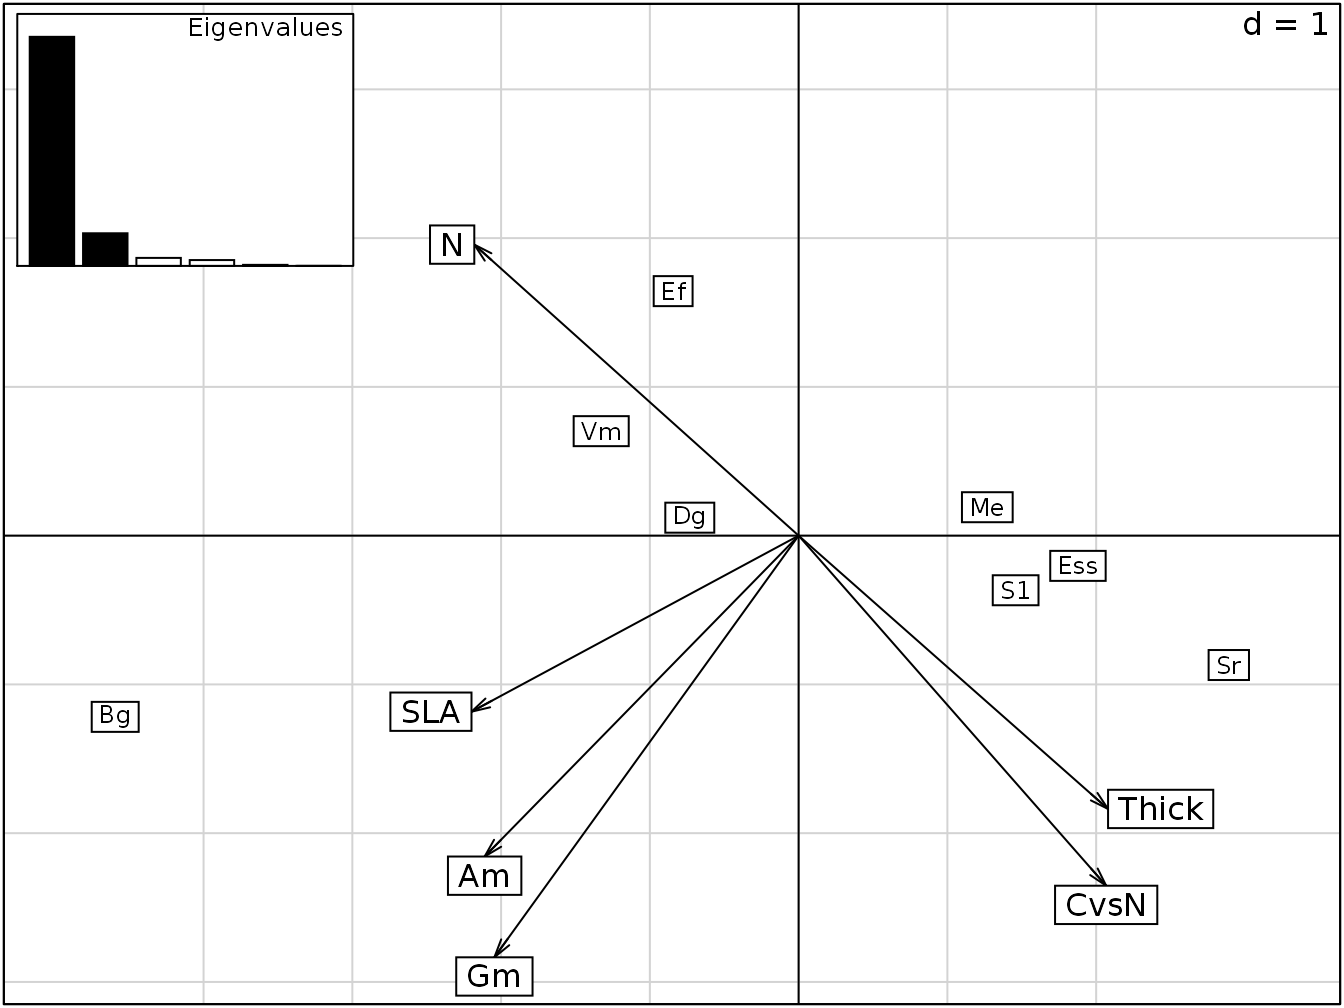
\includegraphics[width=0.8\linewidth]{MesuresBD_files/figure-latex/PCAFFig-1} 

}

\caption{Analyse en composante principale des traits foliaires}\label{fig:PCAFFig}
\end{SCfigure}

\normalsize

\texttt{pcaf} (figure \ref{fig:PCAFFig}) est une liste qui contient les résultats de l'ACP, à utiliser pour la classification:

\scriptsize

\begin{Shaded}
\begin{Highlighting}[]
\CommentTok{# CAH Ward des traits foliaires}
\NormalTok{hf <-}\StringTok{ }\KeywordTok{hclust}\NormalTok{(}\KeywordTok{dist}\NormalTok{(pcaf}\OperatorTok{$}\NormalTok{tab), }\StringTok{"ward.D"}\NormalTok{)}
\end{Highlighting}
\end{Shaded}

\normalsize

Code R pour la figure \ref{fig:PCAFFig}:

\scriptsize

\begin{Shaded}
\begin{Highlighting}[]
\KeywordTok{scatter}\NormalTok{(pcaf)}
\end{Highlighting}
\end{Shaded}

\normalsize

\scriptsize

\begin{SCfigure}

{\centering 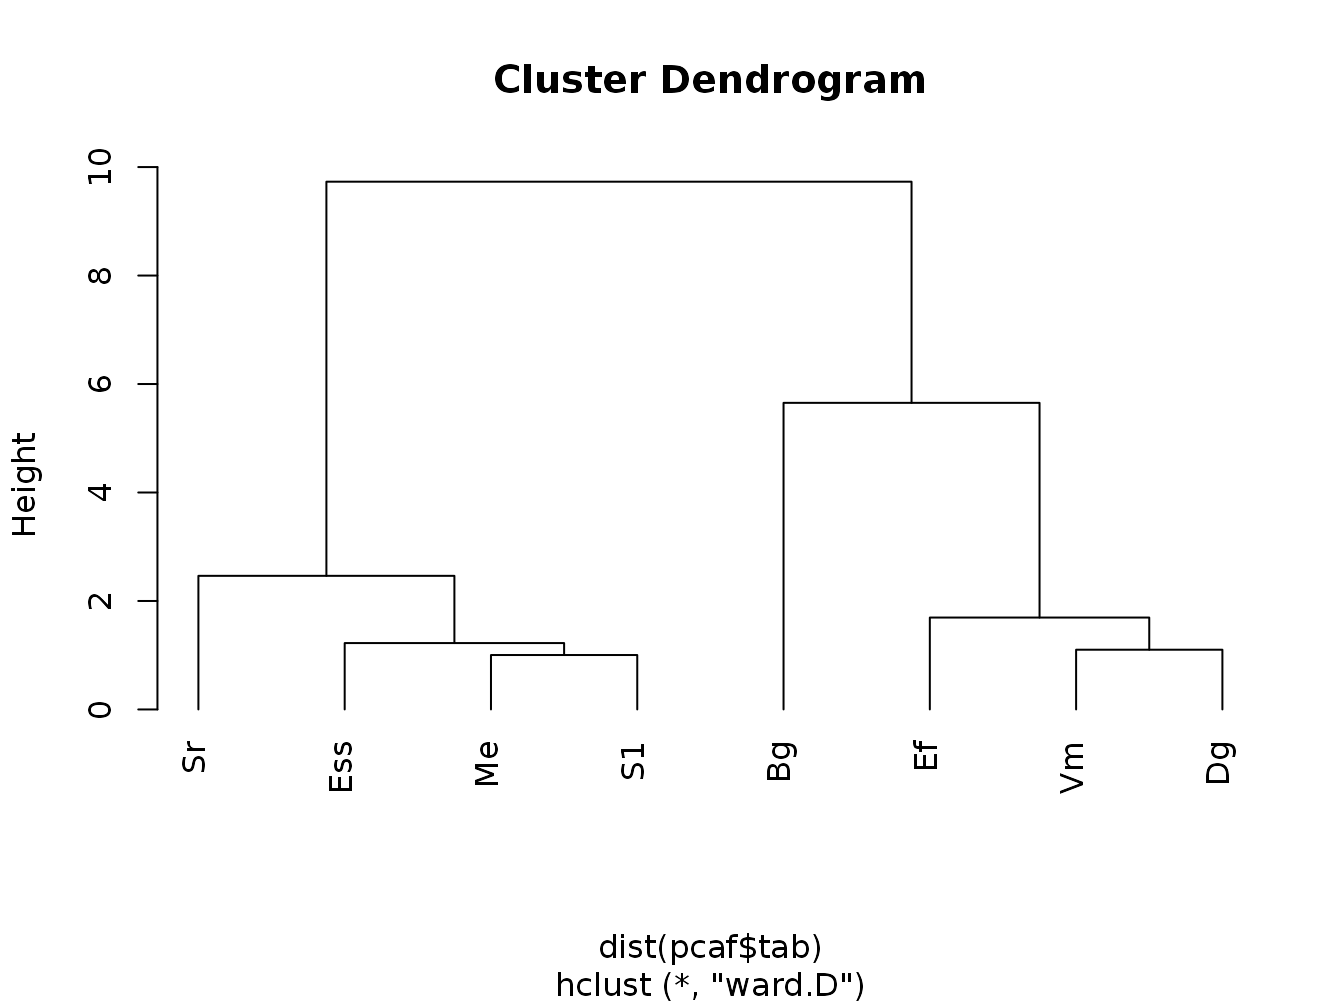
\includegraphics[width=0.8\linewidth]{MesuresBD_files/figure-latex/HclustFig-1} 

}

\caption{Arbre phylogénétique issu de la classification automatique.}\label{fig:HclustFig}
\end{SCfigure}

\normalsize

Le résultat de la classification est un objet \texttt{hclust} (figure \ref{fig:HclustFig} qui doit être transformé en \texttt{phylog} pour la suite de l'analyse:

\scriptsize

\begin{Shaded}
\begin{Highlighting}[]
\CommentTok{# Transformation de l'arbre du format hclust au format phylog}
\NormalTok{phyf <-}\StringTok{ }\KeywordTok{hclust2phylog}\NormalTok{(hf)}
\end{Highlighting}
\end{Shaded}

\normalsize

Code R pour la figure \ref{fig:HclustFig}:

\scriptsize

\begin{Shaded}
\begin{Highlighting}[]
\KeywordTok{plot}\NormalTok{(hf, }\DataTypeTok{h =} \DecValTok{-1}\NormalTok{)}
\end{Highlighting}
\end{Shaded}

\normalsize

Le résultat est en figure \ref{fig:PhylogRaoFig}.



\scriptsize

\begin{SCfigure}

{\centering 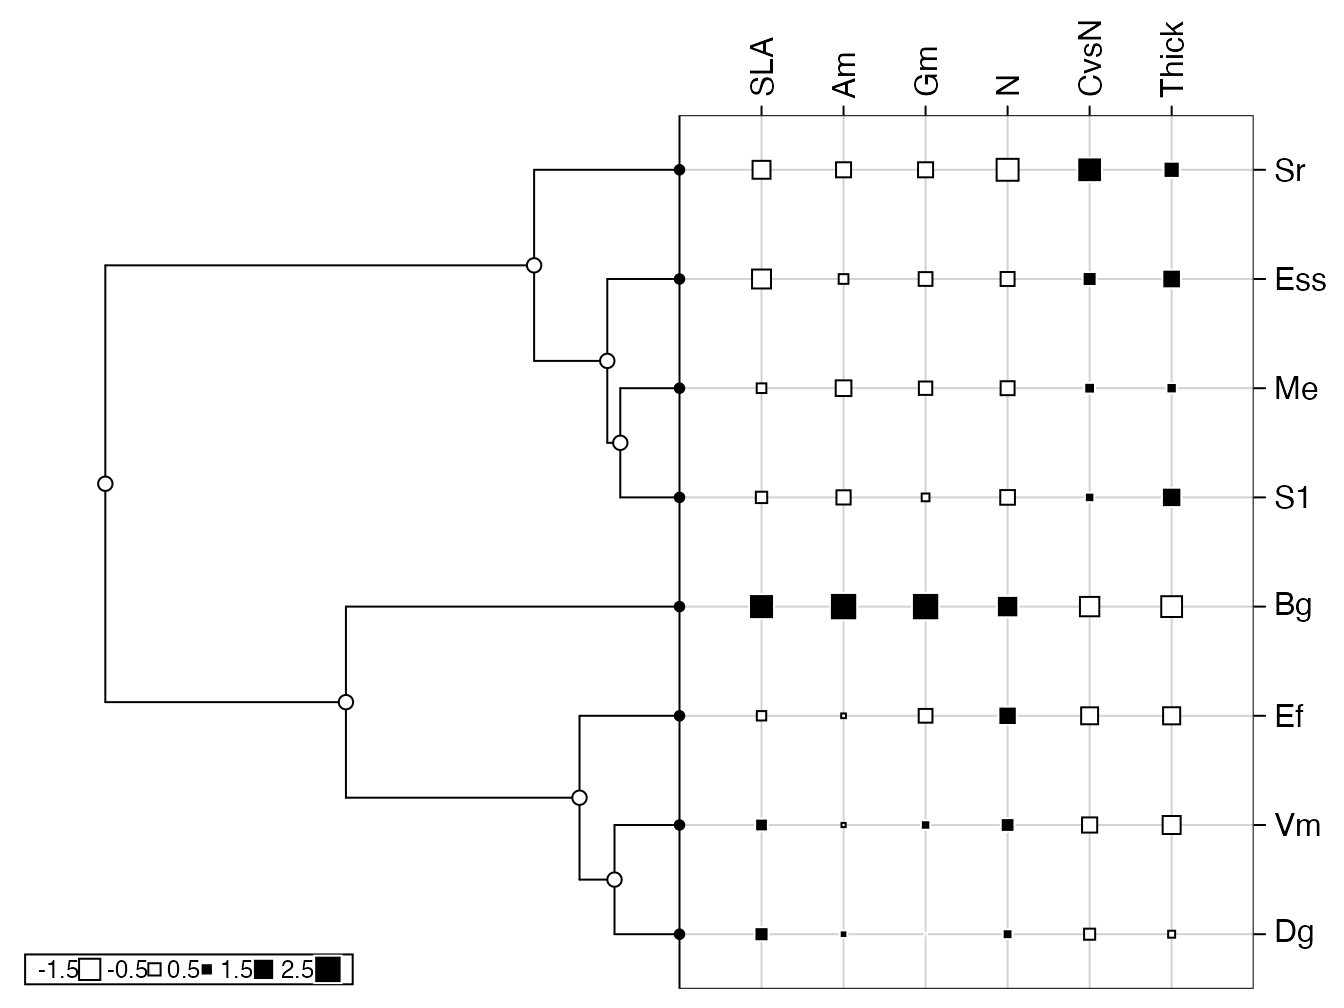
\includegraphics[width=0.8\linewidth]{MesuresBD_files/figure-latex/PhylogRaoFig-1} 

}

\caption{Présentation de l'arbre phylogénétique avec la contribution de chacune des variables.}\label{fig:PhylogRaoFig}
\end{SCfigure}

\normalsize

Code R pour la figure \ref{fig:PhylogRaoFig}:

\scriptsize

\begin{Shaded}
\begin{Highlighting}[]
\KeywordTok{table.phylog}\NormalTok{(pcaf}\OperatorTok{$}\NormalTok{tab[}\KeywordTok{names}\NormalTok{(phyf}\OperatorTok{$}\NormalTok{leaves), ], phyf)}
\end{Highlighting}
\end{Shaded}

\normalsize

La limite des distances ultramétriques est leur tendance à déformer le jeu de points \autocite{Pavoine2005a}.
Dans cet exemple, les deux premiers axes de l'ACP rendent compte de presque toute l'inertie.
Le nuage de points est pratiquement contenu dans un plan alors que sa représentation en distance ultramétrique est une hypersphère en 7 dimensions.

Le calcul de l'originalité des espèces utilise la fonction \texttt{originality} (figure \ref{fig:originalityFig}).

\scriptsize

\begin{SCfigure}

{\centering 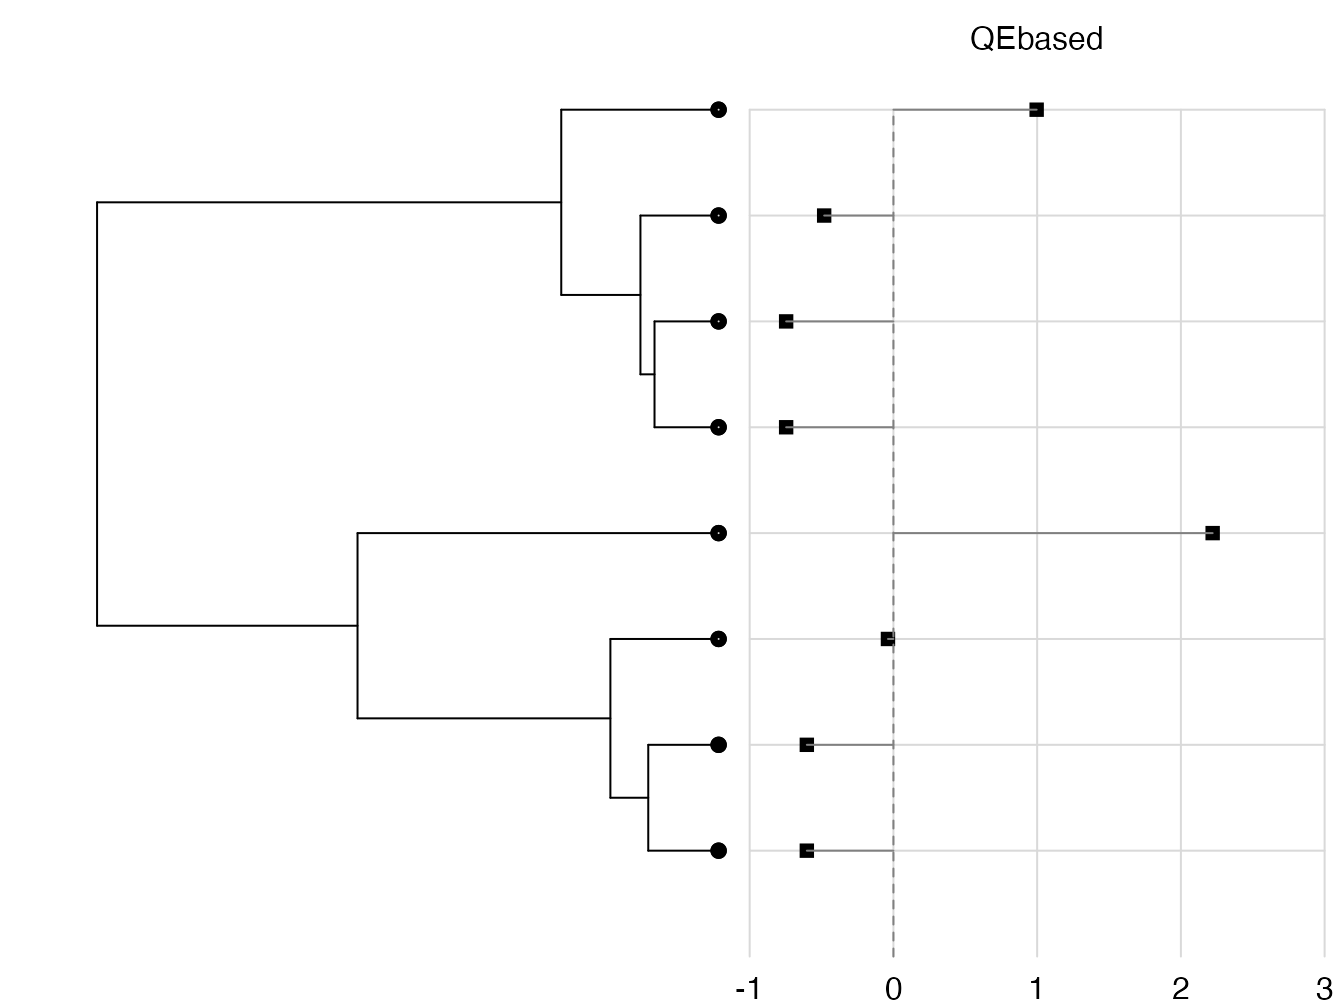
\includegraphics[width=0.8\linewidth]{MesuresBD_files/figure-latex/originalityFig-1} 

}

\caption{Originalité des espèces.}\label{fig:originalityFig}
\end{SCfigure}

\normalsize

Code R pour la figure \ref{fig:originalityFig}:

\scriptsize

\begin{Shaded}
\begin{Highlighting}[]
\KeywordTok{dotchart.phylog}\NormalTok{(phyf, }\KeywordTok{originality}\NormalTok{(phyf, }\DecValTok{5}\NormalTok{))}
\end{Highlighting}
\end{Shaded}

\normalsize

La fonction a pour paramètres l'objet \texttt{phylog} contenant la classification et le numéro de la méthode de calcul à utiliser, 5 pour l'entropie quadratique.
Sa représentation graphique est faite par \texttt{dotchart.phylog}:

L'originalité ne repose que sur l'arbre, pas sur la fréquence des espèces.

Si la distance utilisée n'est pas ultramétrique, il existe plusieurs distributions possibles d'espèces qui maximisent la diversité \autocite{Pavoine2009}, le concept d'originalité n'a pas de sens dans ce cas.

La valeur de l'entropie quadratique dépend de la hauteur de l'arbre.
Plusieurs normalisations ont été proposées: par sa valeur maximale ou par la diversité de Simpson (correspondant à un arbre dont toutes les espèces seraient équidistantes) \autocite{Ricotta2005c}, ou en fixant la hauteur de l'arbre à 1 \autocite{Marcon2014b}.

\hypertarget{diversituxe9-et-moyenne}{%
\section{Diversité et moyenne}\label{diversituxe9-et-moyenne}}

\textcite{Garnier2004} définissent la moyenne pondérée d'un trait à l'échelle de la communauté (CWM: \emph{Community Weigthed Mean}), simplement égal à la moyenne de la valeur du trait pondérée par la fréquence des espèces:

\begin{equation}
  \label{eq:CWM}
  \mathit{CWM} = \sum_s{p_s y_s}.
\end{equation}

CWM n'est pas une mesure de diversité fonctionnelle, bien qu'il ait été utilisé parfois en tant que tel \autocite{Lavorel2008}, mais une mesure de la composition de la communauté.
CWM peut être étendu à plusieurs traits: le vecteur formé par les valeurs de CWM pour chaque trait correspond au centre de gravité de la communauté représentée dans l'espace des traits.
L'entropie quadratique de Rao mesure la dispersion des espèces autour de ce point: les deux mesures se complètent donc \autocite{Ricotta2011}.

\hypertarget{variations-sur-lentropie-quadratique}{%
\section{Variations sur l'entropie quadratique}\label{variations-sur-lentropie-quadratique}}

\textcite{Izsak2011} proposent deux variantes de l'indice de Rao dans lesquelles la distance entre espèces dépend de leurs probabilités:

\begin{equation}
  \label{eq:L1}
  L_1 = \sum_{s}{\sum_{t}{p_{s}p_{t}{\left(p_{s}-p_{t}\right)}^2}};
\end{equation}

\begin{equation}
  \label{eq:L2}
  L_2=\sum_{s}{\sum_{t}{p_{s}p_{t}{\left(\ln{p_{s}}-\ln{p_{t}}\right)}^2}}.
\end{equation}

Ces indices sont proposés pour leurs propriétés mathématiques, assurant l'existence de sa décomposition, sans support écologique bien établi.

\(\mathbf{\Delta}\) est la matrice de dissimilarité dont les éléments sont \(\delta_{s,t}\), la dissimilarité entre l'espèce \(s\) et l'espèce \(t\).
R. C. Guiasu et S. Guiasu \autocite*{Guiasu2011,Guiasu2012} proposent l'indice \(\mathit{{GS}_{D}}\) pour ses propriétés mathématiques et fournissent sa décomposition:

\begin{equation}
  \label{eq:Guiasu}
  \mathit{{GS}_{D}}=\sum_{s}{\sum_{t}{\delta_{s,t}p_{s}}}p_{t}\left(1-p_{s}p_{t}\right).
\end{equation}

\hypertarget{diversituxe9-fonctionnelle-de-chiu-et-chao}{%
\section{Diversité fonctionnelle de Chiu et Chao}\label{diversituxe9-fonctionnelle-de-chiu-et-chao}}

\textcite{Chiu2014b} proposent de pondérer l'entropie quadratique par la distance entre les paires d'espèces et obtiennent un nombre de Hill permettant de mesurer la diversité fonctionnelle à partir d'une matrice de dissimilarité:

\begin{equation}
  \label{eq:Chiu2014bDq}
  ^{q}\!D\left(Q\right)
  = \left[\sum_s{\sum_t{\frac{\delta_{s,t}}{Q}\left(p_s p_t\right)^q}}\right]^\frac{1}{2\left(1-q\right)};
\end{equation}

\begin{equation}
  \label{eq:Chiu2014bD1}
  ^{1}\!D\left(Q\right)
  = e^{\frac{1}{2}\left[\sum_s{\sum_t{p_s p_t\frac{\delta_{s,t}}{Q}\ln{p_s p_t}}}\right]}.
\end{equation}

La notation \(^{q}\!D(Q)\) fait référence à l'entropie quadratique \(Q = {^{2}\!\bar{H}}(T)\).
Une approche complémentaire est développée ci-dessous.
Chiu et Chao notent que \(\mathit{{GS}_{D}} = Q - ^{q}\!D(Q)\).

La définition de Chiu et Chao revient à calculer l'entropie des paires d'individus à partir de la fonction d'information
\[I(p_s p_t) = \ln_q[\frac{(\frac{\delta_{s,t}}{Q})^{\frac{1}{1-q}}}{p_s p_t}]\]
pour \(q \ne 1\) et
\[I(p_s p_t) = \ln[\frac{1}{(p_s p_t)^{\frac{\delta_{s,t}}{Q}}}]\]
pour \(q=1\).
Le nombre effectif de paires est \([^{q}\!D(Q)]^2\). Le nombre effectif d'espèces est donc \(^{q}\!D(Q)\).

Le nombre effectif de paires est le nombres de paires équifréquentes dont la distance entre les deux espèces est \(Q\). Le problème de cette approche est que les paires constituées de la même espèce doivent aussi avoir une distance \(\delta_{s,s}\) égale à \(Q\). Chiu et Chao considèrent ce point comme la possibilité de prendre en compte la variabilité intraspécifique, mais elle doit être identique à la variabilité interspécifique, ce qui n'est pas très convaincant. En absence de variabilité intraspécifique, Chiu et Chao redéfinissent la distance de référence: \(\delta_{s,s}=0\) et \(\delta_{s,t}=(\frac{D}{D-1})Q\). Il n'est donc pas possible de comparer le nombre effectif d'espèces de deux communautés différentes puisque la définition même du nombre effectif dépend de la diversité, ce qui invalide cette définition de la diversité fonctionnelle.

Enfin, cette définition de la diversité ne respecte pas le principe de \textcite{Solow1993} selon lequel le remplacement d'une partie des effectifs d'une espèce par le même nombre d'individus d'une espèce différente mais fonctionnellement identique ne doit pas faire varier la diversité \autocite{Botta-Dukat2017}.

\hypertarget{sec:HpI1}{%
\section{\texorpdfstring{\(H_p\) et \(I_1\)}{H\_p et I\_1}}\label{sec:HpI1}}

Simultanément, \textcite{Pavoine2009a} et \textcite{Allen2009} ont proposé la généralisation de l'indice de Shannon à la diversité phylogénétique.
La présentation de Allen et al.~est donnée ici, celle de Pavoine et al., plus générale, sera détaillée dans le paragraphe suivant.

\scriptsize

\begin{SCfigure}

{\centering 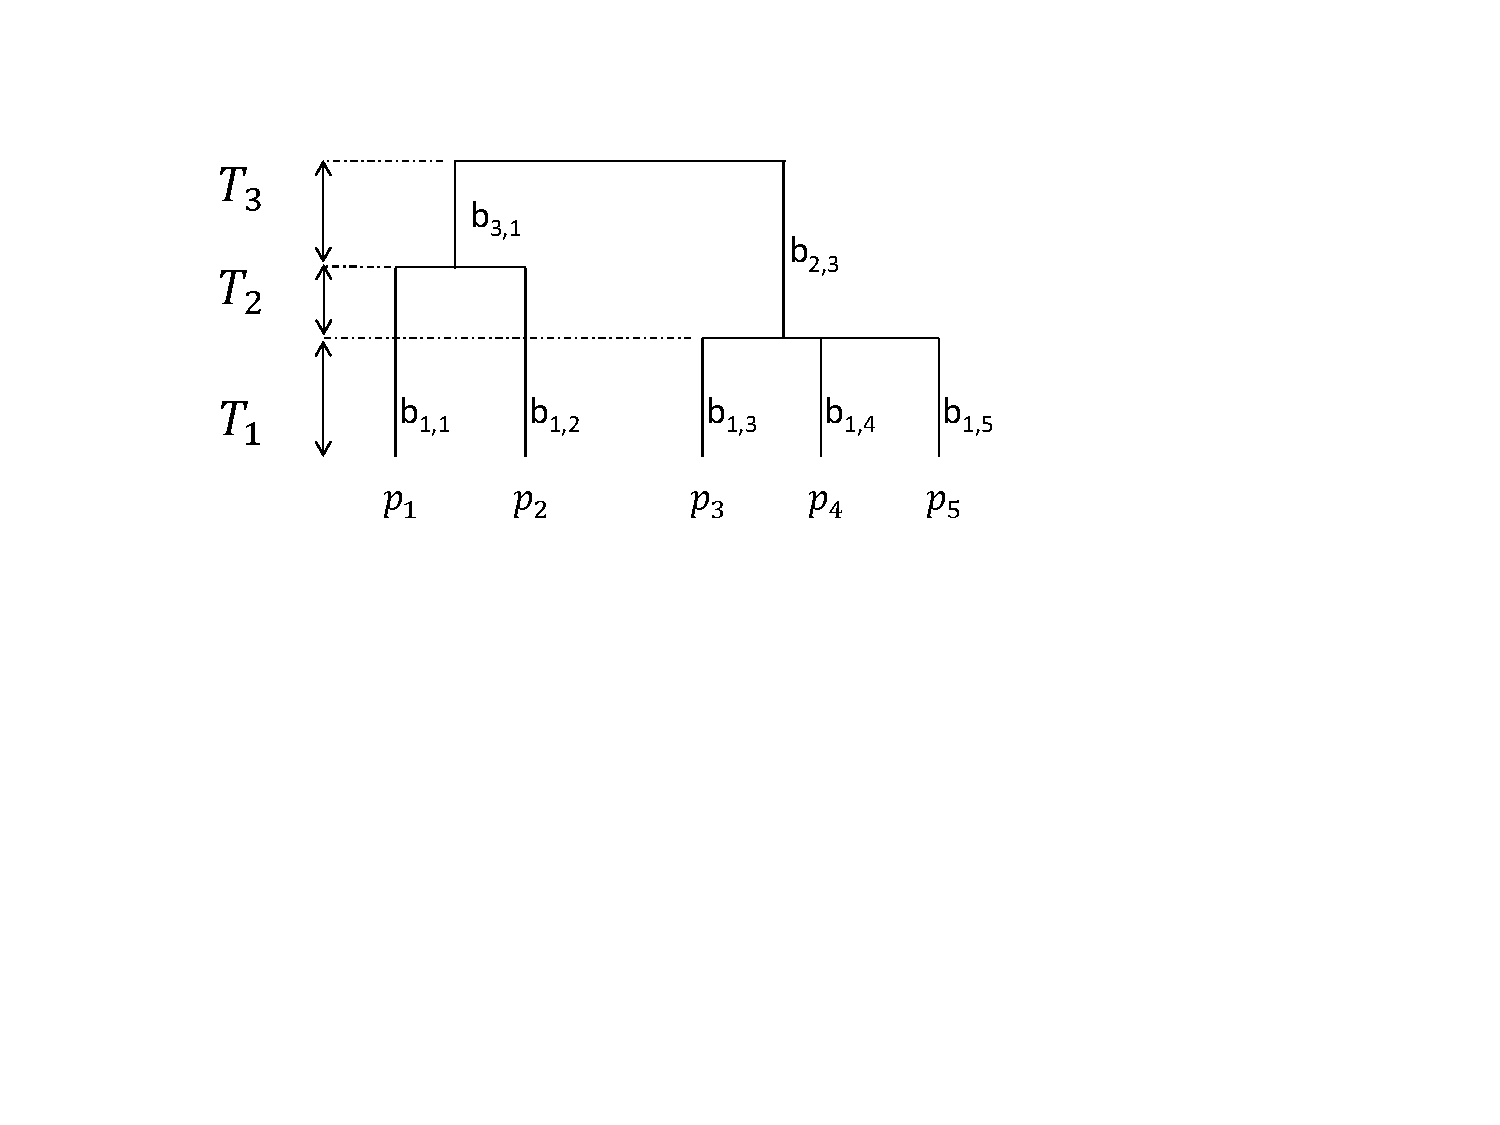
\includegraphics[width=0.8\linewidth]{images/ArbreA} 

}

\caption{Arbre phylogénétique ou fonctionnel hypothétique.}\label{fig:ArbreA2}
\end{SCfigure}

\normalsize

Étant donné une phylogénie, comme celle de la figure \ref{fig:ArbreA2}, on définit une branche \(b_{k,l}\) comme un segment terminé par une feuille (au bas de l'arbre) ou un noeud (dans l'arbre).
\(k\) indique la période de l'arbre à laquelle la branche se termine, \(l\) le numéro d'ordre.
Une branche n'existe que si elle se termine effectivement par un noeud ou une feuille: il n'y a pas de branche \(b_{2,1}\) par exemple.
Sa probabilité \(p(b_{k,l})\) est la somme des probabilités des feuilles de la branche, c'est-à-dire \(u_{k,l}\), et \(l(b)\) est sa longueur.
Sur la figure, la branche commençant en haut de l'arbre et se terminant au noeud réunissant les espèces 3 à 5 a une valeur \(p(b_{2,3})\) égale à la somme des probabilités d'occurrence des espèces 3 à 5 alors que \(p(b_{1,1})\) est seulement la probabilité de l'espèce 1.
Leurs longueurs respectives sont \(T_2+T_3\) et \(T_1+T_2\).
L'arbre possède 7 branches.

L'indice d'entropie phylogénétique est

\begin{equation}
  \label{eq:Hp}
  H_p =-\sum_{b}{l(b)p(b)\ln{p}(b)}.
\end{equation}

Dans un arbre parfaitement régulier, toutes les branches sont de longueur 1 et \(H_p\) est l'indice de Shannon.

\hypertarget{chap:Phyloentropie}{%
\chapter{Entropie phylogénétique}\label{chap:Phyloentropie}}

\scriptsize

\begin{Essentiel}
L'entropie phylogénétique est la moyenne de l'entropie HCDT le long d'un
arbre phylogénétique. Son estimation est simplement celle de l'entropie
HCDT à chaque période de l'arbre. Elle va de pair avec la diversité
phylogénétique qui est son nombre effectif d'espèces, c'est-à-dire le
nombre d'espèces équiprobables, dans un arbre où toutes les espèces
descendraient d'un ancêtre unique, dont l'entropie serait la même que
celle de la communauté réelle. Dans un tel arbre, la diversité
phylogénétique se réduit à la diversité neutre.
\end{Essentiel}

\normalsize

L'entropie HCDT peut être étendue pour définir une mesure de diversité prenant en compte l'histoire évolutive des espèces.

\hypertarget{guxe9nuxe9ralisation-de-lentropie-hcdt}{%
\section{Généralisation de l'entropie HCDT}\label{guxe9nuxe9ralisation-de-lentropie-hcdt}}

\textcite{Pavoine2009} découpent l'arbre phylogénétique en périodes.
À partir de la racine de l'arbre, une nouvelle période est définie à chaque ramification d'une branche quelconque.
Les débuts et fins de périodes sont notés \(t_k\), la racine de l'arbre est fixée à \(t_0=0\).
L'arbre est ultramétrique.

Nous suivrons plutôt les notations de \textcite{Chao2010} en numérotant les périodes à partir du présent et en notant \(T_k\) leur durée.
Figure \ref{fig:Arbre}, la première période se termine quand les branches des espèces 3 à 5 se rejoignent.
L'arbre comprend \(K=3\) périodes.



\scriptsize

\begin{SCfigure}

{\centering 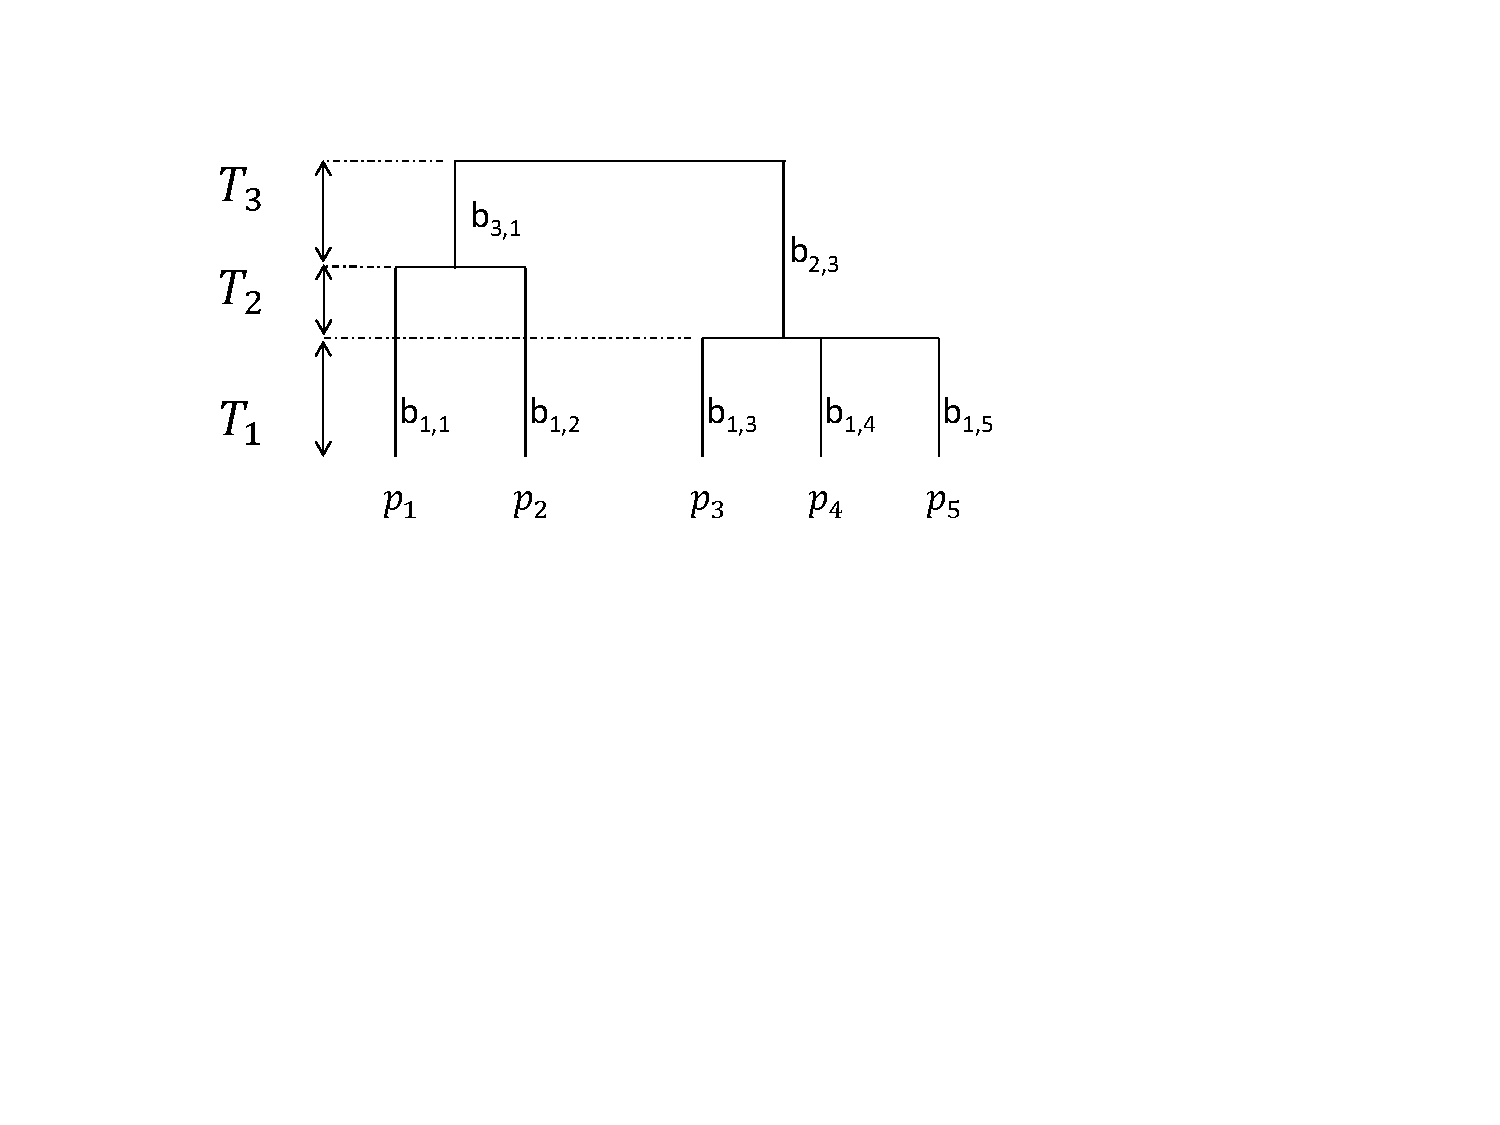
\includegraphics[width=0.8\linewidth]{images/ArbreA} 

}

\caption{Arbre phylogénétique ou fonctionnel hypothétique. 5 espèces sont présentes (\(S=5\)), leurs probabilités notées \(p_1\) à \(p_5\). Les noms des branches sont affichés.}\label{fig:ArbreA5}
\end{SCfigure}

\normalsize

L'entropie HCDT (\(^{q}\!H\) de l'équation \eqref{eq:HCDT}) est calculée à chaque période.
Figure \ref{fig:ArbreA5}, à la deuxième période (\(T_2\)), l'arbre a trois feuilles, avec des probabilités égales à celle des espèces 1 et 2 et la somme de celles des espèces 3 à 5.
\(^{q}\!H\) peut être calculée avec ces valeurs de probabilités.
On notera cette valeur d'entropie \(^{q}_{k}\!H\) où \(k\) est le quantième de la période.

L'indice \(I_q\) de Pavoine et al.~est la somme des \(^{q}_{k}\!H\) pondérée par la durée de chaque période.
Nous le normalisons par la hauteur totale de l'arbre (\(T\)) pour définir \(^{q}\!\bar{H}(T)\):

\begin{equation}
  \label{eq:Hbarq}
  ^{q}\!\bar{H} \left( T \right)=\sum_{k=1}^K{\frac{T_k}{T}^{q}_{k}\!H}.
\end{equation}

Dans un arbre parfaitement régulier, toutes les branches sont de longueur 1, il n'y a qu'une seule période, et \(I_q={^{q}\!H}\).

\textcite{Shimatani2001} puis \textcite{Ricotta2005e} avaient montré que l'indice de Rao est la somme pondérée sur chaque période de l'indice de Simpson, c'est-à-dire l'égalité \eqref{eq:Hbarq} pour le cas particulier \(q=2\).

Les indices \(^{q}\!\bar{H}(T)\) généralisent les mesures d'entropie classique à la diversité phylogénétique: \(T[^{0}\!\bar{H}(T)+1]\) est égal à PD ou FD, \(^{1}\!\bar{H}(T)\) est \(H_p\) et \(^2{\bar{H}(T)}\) est l'indice de Rao.
On peut les interpréter intuitivement comme une somme pondérée par la longueur des périodes des valeurs de l'entropie à chaque période.
À la dernière période (près des feuilles), toutes les classes sont présentes, la diversité est donc maximale.
En remontant dans l'arbre, les classes se confondent et la diversité diminue progressivement.
Deux classes peu distantes, comme les espèces 3 à 5 de la figure \ref{fig:ArbreA5}, apportent peu de diversité supplémentaire par rapport à une situation où les deux espèces seraient confondues (et leurs effectifs ajoutés), contrairement aux espèces 1 et 2.

\hypertarget{sec:phyloEstimation}{%
\section{Estimation}\label{sec:phyloEstimation}}

La correction du biais d'estimation applicable à l'entropie généralisée l'est aussi à chaque période de l'arbre.
Les biais sont de moins en moins importants quand on se rapproche de la racine de l'arbre: il est de moins en moins probable de ne pas observer une classe quand les classes sont de plus en plus vastes.

Le package \emph{entropart} fournit la fonction \texttt{PhyloEntropy} pour calculer \(^{q}\!\bar{H}(T)\) à partir d'un vecteur de probabilité ou d'abondances.
Dans le dernier cas, la correction de \texttt{Tsallis} est appliquée à chaque période.

Exemple: le package contient les données d'inventaire de deux hectares du dispositif de Paracou et la taxonomie des espèces concernées.
Le calcul de l'indice de Rao, corrigé du biais d'estimation utilise le code suivant:

\scriptsize

\begin{Shaded}
\begin{Highlighting}[]
\KeywordTok{data}\NormalTok{(Paracou618)}
\KeywordTok{PhyloEntropy}\NormalTok{(Paracou618.MC}\OperatorTok{$}\NormalTok{Ns, }\DecValTok{2}\NormalTok{, Paracou618.Taxonomy)}
\end{Highlighting}
\end{Shaded}

\begin{verbatim}
## $Distribution
## [1] "Paracou618.MC$Ns"
## 
## $Function
## [1] "PhyloEntropy"
## 
## $Tree
## [1] "Paracou618.Taxonomy"
## 
## $Normalized
## [1] TRUE
## 
## $Cuts
##         1         2         3 
## 0.9863189 0.9709766 0.9232516 
## 
## $Corrections
##         1         2         3 
## "UnveilJ" "UnveilJ" "UnveilJ" 
## 
## $Total
## [1] 0.9601824
## 
## $Type
## [1] "alpha or gamma"
## 
## $Order
## [1] 2
## 
## $Correction
## [1] "Best"
## 
## attr(,"class")
## [1] "PhyloEntropy" "PhyloValue"
\end{verbatim}

\normalsize

La fonction retourne la valeur de \(^{q}_{k}\!H\) dans chaque intervalle (l'arbre est ici une taxonomie espèce-genre-famille, correspondant aux limites des périodes (\texttt{Cuts}) 1, 2 et 3 dont l'entropie va en décroissant) et la valeur de \(^{q}\!\bar{H}(T)\).

\hypertarget{sec:phyloEntopieDiv}{%
\section{Entropie et diversité}\label{sec:phyloEntopieDiv}}

La diversité phylogénétique est le nombre d'espèces équifréquentes et dont la distance à toutes les autres dans la phylogénie est maximale, dont l'entropie serait égale à l'entropie observée.

La possibilité de choisir comme distance de référence entre espèces une valeur inférieure à la distance maximale est discutée par \textcite{Ricotta2014a} pour la diversité fonctionnelle: sa signification biologique est liée à l'espace fonctionnel disponible pour la communauté, qui peut être trop réduit pour permettre la coexistence d'espèces dont la dissimilarité serait maximale.

L'entropie \(^{q}\!\bar{H}(T)\) peut être transformée en diversité \autocite{Marcon2014a} de la même façon que \(^{q}\!D = e^{^{q}\!H}\):

\begin{equation}
  \label{eq:DbarqT}
  ^{q}\!\bar{D}\left(T\right)=e^{^{q}\!\bar{H}\left(T\right)}_q.
\end{equation}

Le nombre effectif d'espèces de l'entropie de Rao, \({^{2}\!\bar{D}}(T)=\frac{1}{[1-{^{2}\!\bar{H}}(T)]}\) a été établi par \textcite{Ricotta2009}.

\textcite{Chao2010} obtiennent ce résultat sans recourir explicitement à l'entropie, mais en faisant le même calcul:

\begin{equation}
  \label{eq:DbarqChao}
  {^{q}\!\bar{D}} \left( T \right)
  =\left( \sum_b{\frac{l(b)}{T} p(b)^q} \right)^{\frac{1}{1-q}}.
\end{equation}

La somme est sur l'ensemble des branches de l'arbre, défini de façon identique à celle de \textcite{Allen2009} \ref{sec:HpI1}.

Les entropies ont un comportement linéaire: elles s'additionnent tout au long de l'arbre pour donner \(^{q}\!\bar{H}(T)\).
Les diversités \(^{q}_{k}\!D\) calculées à chaque période ne peuvent pas être sommées sur le modèle de l'équation \eqref{eq:Hbarq}: \(^{q}\!\bar{D}(T)\) n'est \emph{pas} la moyenne pondérée des diversités aux différentes périodes, sauf dans le cas particulier \(q=1\) où, comme pour la décomposition de l'indice de Shannon, il en est la moyenne géométrique pondérée.

La fonction \texttt{PhyloDiversity} de \emph{entropart} permet de calculer \(^{q}\!\bar{D}(T)\) avec ou sans correction de biais, selon qu'elle traite un vecteur d'abondances ou de probabilités.
À la suite de l'exemple précédent, les résultats sont présentés sous forme de diversité au lieu d'entropie:

\scriptsize

\begin{Shaded}
\begin{Highlighting}[]
\KeywordTok{PhyloDiversity}\NormalTok{(Paracou618.MC}\OperatorTok{$}\NormalTok{Ns, }\DecValTok{2}\NormalTok{, Paracou618.Taxonomy)}
\end{Highlighting}
\end{Shaded}

\begin{verbatim}
## $Distribution
## [1] "Paracou618.MC$Ns"
## 
## $Function
## [1] "bcPhyloDiversity"
## 
## $Tree
## [1] "Paracou618.Taxonomy"
## 
## $Normalized
## [1] TRUE
## 
## $Cuts
##        1        2        3 
## 73.09335 34.45501 13.02960 
## 
## $Corrections
##         1         2         3 
## "UnveilJ" "UnveilJ" "UnveilJ" 
## 
## $Total
## [1] 25.11451
## 
## $Type
## [1] "alpha or gamma"
## 
## $Order
## [1] 2
## 
## $Correction
## [1] "Best"
## 
## attr(,"class")
## [1] "PhyloDiversity" "PhyloValue"
\end{verbatim}

\normalsize

\hypertarget{diversituxe9-individuelle}{%
\section{Diversité individuelle}\label{diversituxe9-individuelle}}

La construction de la diversité fonctionnelle ou phylogénétique n'implique pas de regrouper les individus par espèces: chaque catégorie peut se réduire à un individu si des données individuelles moléculaires ou de traits sont disponibles.

Le regroupement des individus en une espèce revient simplement à considérer leur distance comme nulle.
Diviser une espèce en deux espèces infiniment proches revient seulement à créer une période supplémentaire dans l'arbre, de longueur infinitésimale; en d'autres termes, la mesure de diversité est continue face au regroupement.
Cette propriété permet de limiter les conséquences du problème de l'espèce: séparer les individus d'une espèce en deux espèces proches dans l'arbre n'a que peu d'effet sur la diversité.

\hypertarget{arbres-non-ultramuxe9triques}{%
\section{Arbres non ultramétriques}\label{arbres-non-ultramuxe9triques}}

\scriptsize

\begin{SCfigure}

{\centering 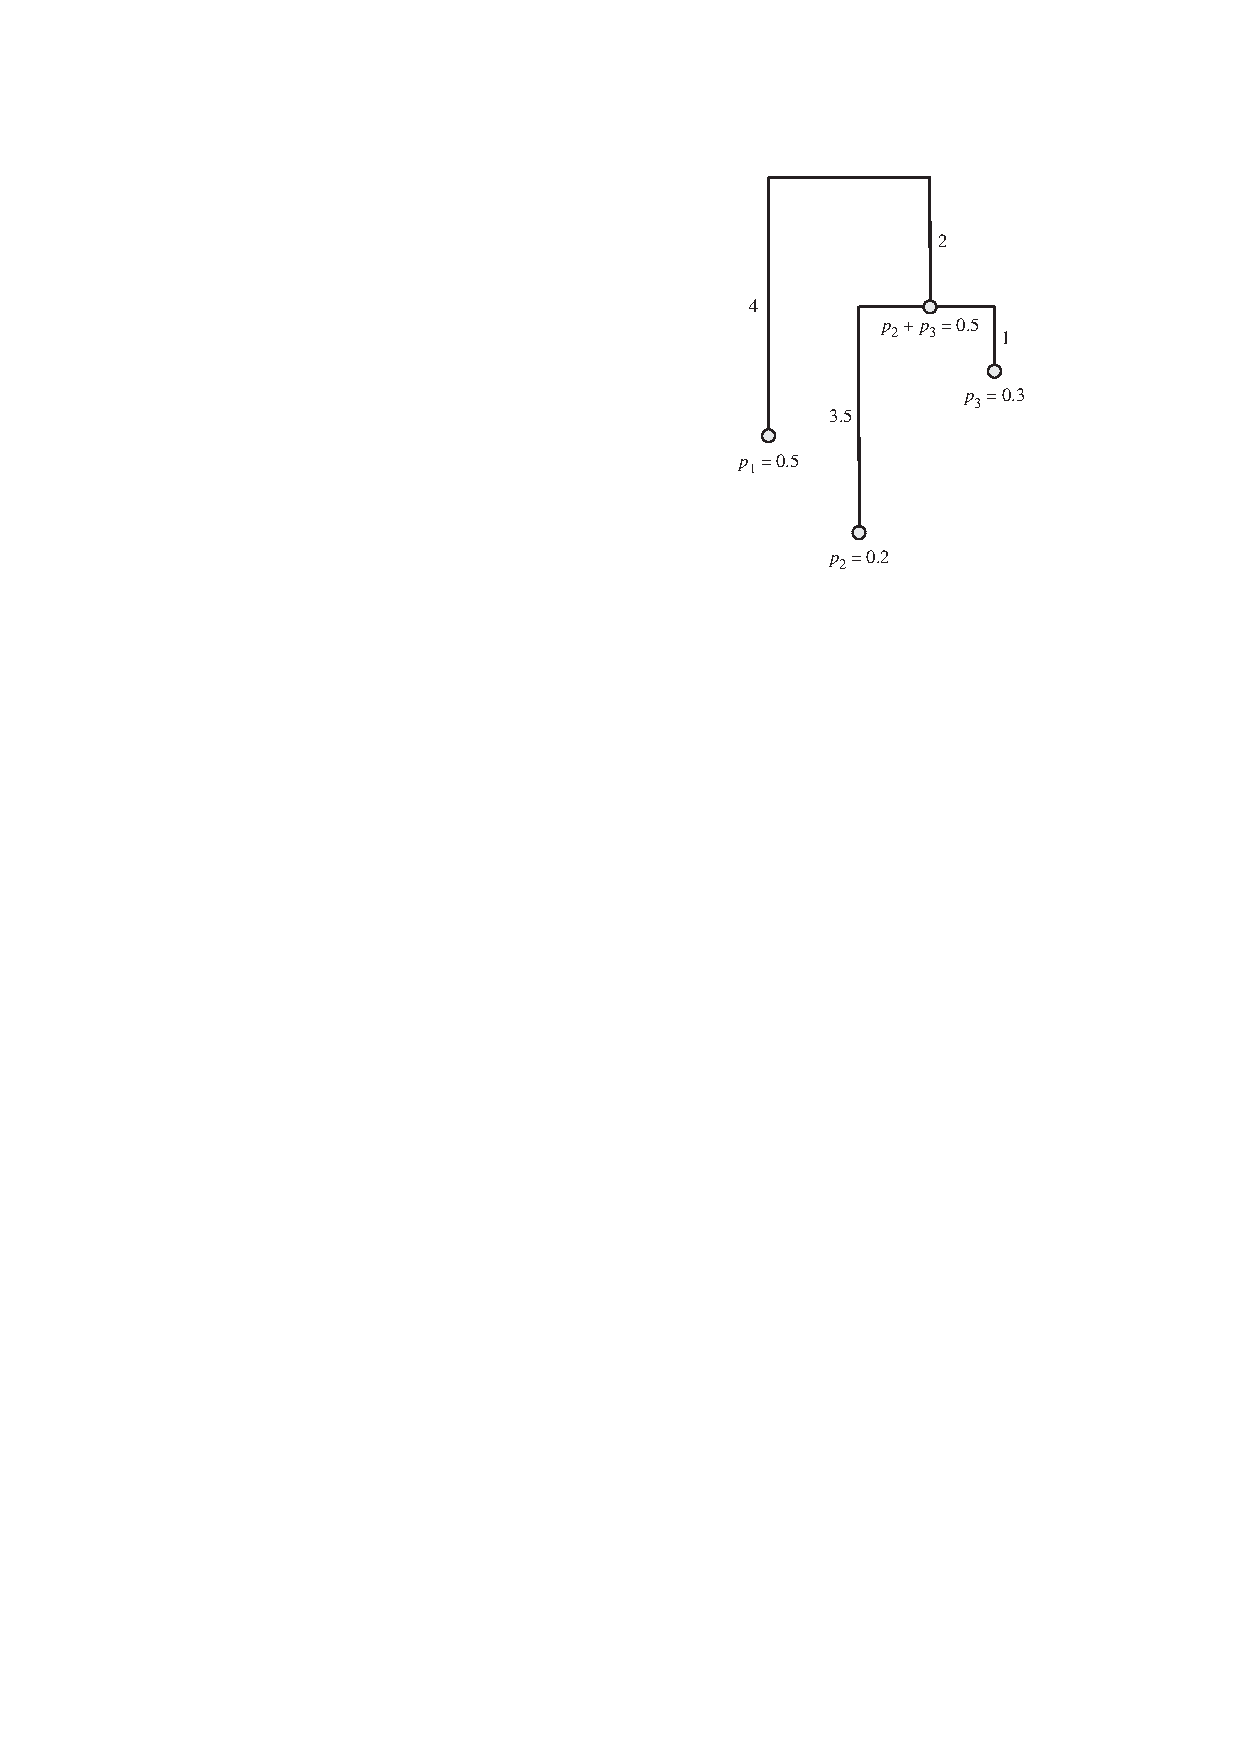
\includegraphics[width=0.4\linewidth]{images/Chao2010} 

}

\caption{Arbre phylogénétique hypothétique non ultramétrique}\label{fig:Chao2010}
\end{SCfigure}

\normalsize

\textcite{Chao2010} définissent la diversité phylogénétique selon l'équation \eqref{eq:DbarqChao} quelle que soit la forme de l'arbre, y compris s'il n'est pas ultramétrique.
Dans ce cas, \(T\) est remplacé par \(\bar{T}\), la longueur moyenne des branches pondérée par la fréquence des espèces.
Cette généralisation est très discutable: son sens n'est pas clair sur le plan de la mesure de la diversité au-delà du parallélisme de la forme mathématique.

L'arbre de la figure \ref{fig:Chao2010} \autocite[figure 1b]{Chao2010} peut être découpé en périodes mais les deux premières (\(T_1\): seule l'espèce 2 est présente; \(T_2\): les espèces 1 et 2 sont présentes) sont incomplètes au sens où la somme des probabilités n'y est pas égale à 1 donc \({\left(\sum{p^q_i}\right)}^{\frac{1}{1-q}}\) ne définit pas une diversité à ces périodes.

\textcite{Pavoine2009} traitent en détail les résultats aberrants que cause un arbre non ultramétrique dans le cas particulier de l'entropie de Rao.
\textcite{Leinster2012} montrent qu'un arbre non ultramétrique implique que la dissimilarité entre les espèces dépende de leur fréquence, ce qui est contradictoire avec le cadre dans lequel la diversité phylogénétique a été définie.

Dans l'état actuel des connaissances, aucune méthode n'est applicable de façon satisfaisante aux arbres non ultramétriques.

\hypertarget{chap:LeinsterCobbold}{%
\chapter{Diversité de Leinster et Cobbold}\label{chap:LeinsterCobbold}}

\scriptsize

\begin{Essentiel}
La diversité de Leinster et Cobbold est l'inverse de la banalité moyenne
des espèces, qui est elle-même la similarité moyenne d'une espèce aux
autres. Elle va de pair avec l'entropie de Ricotta et Szeidl, dont la
fonction d'information est le logarithme déformé de l'inverse la
banalité. La diversité peut être calculée directement à partir de la
distance entre espèces, sans recourir à un dendrogramme intermédiaire
qui déformerait la topologie des espèces.
\end{Essentiel}

\normalsize

À partir de la théorie mathématique des catégories \autocite{Leinster2013}, \textcite{Leinster2012} ont proposé une mesure de diversité applicable à une communauté dont la position des espèces dans un espace multidimensionnel euclidien est connue.
C'est donc une mesure applicable à la diversité fonctionnelle.

\hypertarget{duxe9finitions}{%
\section{Définitions}\label{duxe9finitions}}

\textcite{Leinster2012} proposent une unification des mesures de diversité à partir de la définition de la banalité des espèces.
Une matrice carrée de dimension égale au nombre d'espèces, \(\mathbf{Z}\), décrit par ses valeurs \(z_{s,t}\) la similarité entre l'espèce \(s\) et l'espèce \(t\) comprises entre 0 et 1 (\(z_{s,s}=1\)).

La banalité d'une espèce \(s\) est définie par \(\sum_t{p_t z_{s,t}}\), c'est-à-dire la moyenne pondérée de sa similarité avec toutes les autres espèces: au minimum \(p_s\) si elle est totalement différente des autres (approche de la diversité neutre, \(\mathbf{Z}\) est la matrice identité \(\mathbf{I}_s\)), au maximum 1 si toutes les espèces sont totalement similaires (\(\mathbf{Z}\) ne contient que des 1).
Une espèce rare totalement différente des autres est peu banale.

La moyenne généralisée d'ordre \(r\) \autocite{Hardy1952}, \emph{generalized mean} ou \emph{power mean} en anglais, est définie pour une distribution de valeurs de \(x_s\) dont la probabilité d'occurrence est \(p_s\) par

\begin{equation}
  \label{eq:Hardy1952}
  \bar{x}={\left(\sum_s{p_s x^r_s}\right)}^{\frac{1}{r}}.
\end{equation}



\scriptsize

\begin{SCfigure}

{\centering 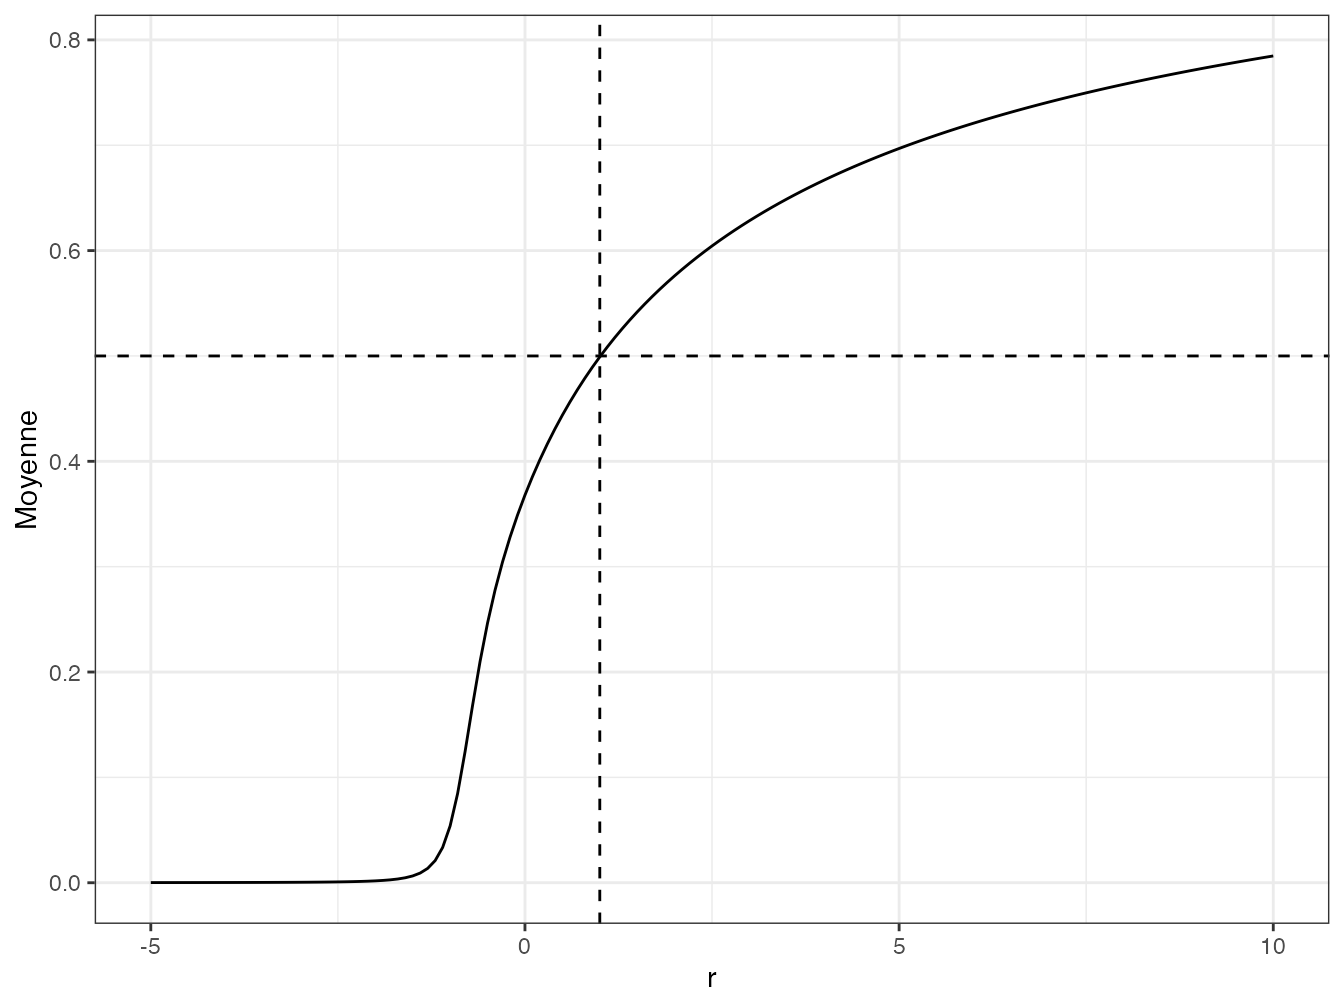
\includegraphics[width=0.8\linewidth]{MesuresBD_files/figure-latex/MoyenneHardyFig-1} 

}

\caption{Moyenne généralisée d'ordre \(r\) (en abscisse) d'une distribution uniforme de 10000 valeurs tirées entre 0 et 1. La moyenne arithmétique 0,5 est obtenue pour \(r=1\). La moyenne généralisée tend vers la plus petite valeur (près de 0) quand \(r\to -\infty\), et vers la plus grande valeur (près de 1) quand \(r\to +\infty\).}\label{fig:MoyenneHardyFig}
\end{SCfigure}

\normalsize

La moyenne généralisée se réduit à la moyenne arithmétique pondérée pour \(r=1\).
Elle donne un fort poids aux petites valeurs de \(x_s\) dans la moyenne pour les faibles valeurs de \(r\) (qui peuvent être négatives), et un fort poids aux grandes valeurs quand \(r\) est grand (figure \ref{fig:MoyenneHardyFig}).

Le code R nécessaire pour réaliser la figure est:

\scriptsize

\begin{Shaded}
\begin{Highlighting}[]
\NormalTok{X <-}\StringTok{ }\KeywordTok{runif}\NormalTok{(}\DecValTok{10000}\NormalTok{)}
\CommentTok{# La moyenne n'est pas définie à r=0, décalage de 10^-8}
\NormalTok{r <-}\StringTok{ }\KeywordTok{seq}\NormalTok{(}\OperatorTok{-}\DecValTok{5}\NormalTok{, }\DecValTok{10}\NormalTok{, }\FloatTok{.1}\NormalTok{) }\OperatorTok{+}\StringTok{ }\FloatTok{1E-8}
\CommentTok{# Préparation des données}
\NormalTok{df <-}\StringTok{ }\KeywordTok{data.frame}\NormalTok{(r, }\DataTypeTok{Moyenne =} \KeywordTok{sapply}\NormalTok{(r, }\ControlFlowTok{function}\NormalTok{(r) (}\KeywordTok{mean}\NormalTok{(X}\OperatorTok{^}\NormalTok{r))}\OperatorTok{^}\NormalTok{(}\DecValTok{1}\OperatorTok{/}\NormalTok{r)))}
\KeywordTok{ggplot}\NormalTok{(df, }\KeywordTok{aes}\NormalTok{(}\DataTypeTok{x =}\NormalTok{ r, }\DataTypeTok{y =}\NormalTok{ Moyenne)) }\OperatorTok{+}
\StringTok{  }\KeywordTok{geom_line}\NormalTok{() }\OperatorTok{+}
\StringTok{  }\KeywordTok{geom_hline}\NormalTok{(}\DataTypeTok{yintercept =} \FloatTok{.5}\NormalTok{, }\DataTypeTok{lty =} \DecValTok{2}\NormalTok{) }\OperatorTok{+}
\StringTok{  }\KeywordTok{geom_vline}\NormalTok{(}\DataTypeTok{xintercept =} \DecValTok{1}\NormalTok{, }\DataTypeTok{lty =} \DecValTok{2}\NormalTok{)}
\end{Highlighting}
\end{Shaded}

\normalsize

La banalité peut s'écrire sous forme matricielle en notant \(\mathbf{p}\) le vecteur des probabilités \(p_s\), on note alors \({\left(\mathbf{Zp}\right)}_s=\sum_t{p_{t}z_{s,t}}\).

La banalité moyenne des espèces de la communauté est calculée en prenant \(r=q-1\):

\begin{equation}
  \label{eq:barZp}
  \left(\overline{{\mathbf{Zp}}}\right)
  = {\left(\sum_s{p_s{\left(\mathbf{Zp}\right)}^{q-1}_s}\right)}^{\frac{1}{q-1}}.
\end{equation}

La diversité de la communauté est simplement l'inverse de la banalité moyenne des espèces:

\begin{equation}
  \label{eq:Dqz}
  ^q\!D^{\mathbf{Z}}={\left(\sum_s{p_s{\left(\mathbf{Zp}\right)}^{q-1}_s}\right)}^{\frac{1}{1-q}}.
\end{equation}

\(^q\!D^{\mathbf{Z}}\) converge vers \(^1\!D^{\mathbf{Z}}\) quand \(q\) tend vers 1:

\begin{equation}
  \label{eq:D1z}
  ^1\!D^{\mathbf{Z}} = \frac{1}{\prod_s{{\left(\mathbf{Zp}\right)}^{p_s}_s}}.
\end{equation}

\hypertarget{diversituxe9-neutre}{%
\section{Diversité neutre}\label{diversituxe9-neutre}}

Leinster et Cobbold montrent que la diversité HCDT est un cas particulier de \(^q\!D^{\mathbf{Z}}\), pour la matrice identité:

\begin{equation}
  \label{eq:DqI}
  ^{q}\!D={^q\!D^{\mathbf{I}}}.
\end{equation}

\hypertarget{diversituxe9-non-neutre}{%
\section{Diversité non neutre}\label{diversituxe9-non-neutre}}

Une mesure de diversité non neutre est obtenue en utilisant une matrice \(\mathbf{Z}\) qui contient l'information sur la similarité entre les espèces.
La dissimilarité entre espèces peut être obtenue à partir des arbres.
L'exemple suivant utilise les données du calcul d'originalité, section \ref{sec:MaxTheorique}.
Pour un arbre de classe \texttt{hclust}, la fonction \texttt{cophenetic} fournit une demi-matrice de distances (classe \texttt{dist}).

\scriptsize

\begin{Shaded}
\begin{Highlighting}[]
\KeywordTok{print}\NormalTok{(}\KeywordTok{cophenetic}\NormalTok{(hf), }\DataTypeTok{digits =} \DecValTok{4}\NormalTok{)}
\end{Highlighting}
\end{Shaded}

\begin{verbatim}
##      Ess    Me    S1    Sr    Vm    Bg    Ef
## Me 1.224                                    
## S1 1.224 1.003                              
## Sr 2.464 2.464 2.464                        
## Vm 9.731 9.731 9.731 9.731                  
## Bg 9.731 9.731 9.731 9.731 5.653            
## Ef 9.731 9.731 9.731 9.731 1.694 5.653      
## Dg 9.731 9.731 9.731 9.731 1.101 5.653 1.694
\end{verbatim}

\normalsize

La matrice doit être normalisée puis transformée en matrice de similarité.
Une transformation simple est 1 moins la dissimilarité (préalablement normalisée pour être comprise entre 0 et 1):

\scriptsize

\begin{Shaded}
\begin{Highlighting}[]
\NormalTok{Dis <-}\StringTok{ }\KeywordTok{cophenetic}\NormalTok{(hf)}
\KeywordTok{print}\NormalTok{((Z <-}\StringTok{ }\DecValTok{1} \OperatorTok{-}\StringTok{ }\KeywordTok{as.matrix}\NormalTok{(Dis}\OperatorTok{/}\KeywordTok{max}\NormalTok{(Dis))), }\DataTypeTok{digits =} \DecValTok{4}\NormalTok{)}
\end{Highlighting}
\end{Shaded}

\begin{verbatim}
##        Ess     Me     S1     Sr     Vm     Bg     Ef     Dg
## Ess 1.0000 0.8742 0.8742 0.7468 0.0000 0.0000 0.0000 0.0000
## Me  0.8742 1.0000 0.8969 0.7468 0.0000 0.0000 0.0000 0.0000
## S1  0.8742 0.8969 1.0000 0.7468 0.0000 0.0000 0.0000 0.0000
## Sr  0.7468 0.7468 0.7468 1.0000 0.0000 0.0000 0.0000 0.0000
## Vm  0.0000 0.0000 0.0000 0.0000 1.0000 0.4191 0.8259 0.8868
## Bg  0.0000 0.0000 0.0000 0.0000 0.4191 1.0000 0.4191 0.4191
## Ef  0.0000 0.0000 0.0000 0.0000 0.8259 0.4191 1.0000 0.8259
## Dg  0.0000 0.0000 0.0000 0.0000 0.8868 0.4191 0.8259 1.0000
\end{verbatim}

\normalsize

La diversité peut être calculée par la fonction \texttt{Dqz} de \emph{entropart}:

\scriptsize

\begin{Shaded}
\begin{Highlighting}[]
\CommentTok{# Vecteur contenant 8 espèces...}
\NormalTok{(effectifs <-}\StringTok{ }\KeywordTok{read.csv2}\NormalTok{(}\StringTok{"data/rao.effectifs.csv"}\NormalTok{, }\DataTypeTok{row.names =} \DecValTok{1}\NormalTok{, }
    \DataTypeTok{header =}\NormalTok{ T))}
\end{Highlighting}
\end{Shaded}

\begin{verbatim}
##     P1 P2 P3 P4
## Ess 97 36 34 61
## Me  62 24 49  4
## S1   4  6  6 75
## Sr  71 78 99 36
## Vm  76 29 34  2
## Bg  58 49 47 19
## Ef   9 34 91 35
## Dg  98 14 95 14
\end{verbatim}

\begin{Shaded}
\begin{Highlighting}[]
\NormalTok{Ps <-}\StringTok{ }\KeywordTok{rowSums}\NormalTok{(effectifs)}\OperatorTok{/}\KeywordTok{sum}\NormalTok{(effectifs)}
\KeywordTok{Dqz}\NormalTok{(Ps, }\DataTypeTok{q =} \DecValTok{2}\NormalTok{, Z)}
\end{Highlighting}
\end{Shaded}

\begin{verbatim}
##     None 
## 2.520938
\end{verbatim}

\normalsize

Dans le cas particulier \(q=2\), \(^2\!D^{\mathbf{Z}}\) est égal à \(^{2}\!\bar{D}(T)\):

\scriptsize

\begin{Shaded}
\begin{Highlighting}[]
\KeywordTok{PhyloDiversity}\NormalTok{(Ps, }\DataTypeTok{q =} \DecValTok{2}\NormalTok{, phyf)}\OperatorTok{$}\NormalTok{Total}
\end{Highlighting}
\end{Shaded}

\begin{verbatim}
##     None 
## 2.520938
\end{verbatim}

\normalsize

Mais ce n'est pas le cas en général.

\hypertarget{entropie-de-ricotta-et-szeidl}{%
\section{Entropie de Ricotta et Szeidl}\label{entropie-de-ricotta-et-szeidl}}

\textcite{Ricotta2006b} ont montré une similitude entre les entropies de Shannon et de Rao en généralisant l'entropie de Shannon en deux temps.
Tout d'abord en remarquant que la probabilité d'occurrence d'une espèce est 1 moins la somme de celle des autres, d'où

\begin{equation}
  \label{eq:Ricotta2006bH1}
  ^{1}\!H = -\sum_s{p_s\ln\left(1-\sum_{t\ne s}{p_t}\right)}.
\end{equation}

\(1-\sum_{t\ne s}{p_t}\) est la banalité de l'espèce \(s\) si on mesure la diversité neutre.
De façon plus générale, \({(\mathbf{Zp})}_s\) peut exprimer cette banalité.
Enfin, l'entropie HCDT peut généraliser l'entropie de Shannon pour définir une mesure \(Q_{\alpha}\) que nous noterons \(^q\!H^{\mathbf{Z}}\) pour la cohérence de nos notations (\(q=\alpha\)):

\begin{equation}
  \label{eq:Ricotta2006bHZ}
  ^q\!H^{\mathbf{Z}} = \sum_s{p_{s}\ln_q{\frac{1}{\left(\mathbf{Zp}\right)_s}}}.
\end{equation}

De façon plus rigoureuse, on peut remarquer que \({(\mathbf{Zp})}_s\) décroît quand \(p_s\) décroît parce que la similarité d'une espèce avec elle-même est maximale.
Une entropie définie à partir d'une fonction d'information de \(p_s\) reste donc une entropie quand on utilise la même fonction d'information sur \({(\mathbf{Zp})}_s\): la fonction reste décroissante et vaut 0 pour \(p_s=1\) puisque \({(\mathbf{Zp})}_s=1\) dans ce cas.
\(^q\!H^{\mathbf{Z}}\) est donc bien une entropie.
La fonction d'information \(\ln_q(1/p_s)\) de l'entropie HCDT \eqref{eq:EntropieHCDT} est simplement remplacée par \(\ln_q(1/{(\mathbf{Zp})}_s)\).

L'entropie de Ricotta et Szeidl étend l'entropie HCDT en utilisant une fonction d'information plus générale, dépendant de la banalité de l'espèce plutôt que de sa seule probabilité, les deux étant égales dans le cas particulier de la diversité neutre.
L'ordre de la diversité \(q\) permet de donner un plus ou moins grand poids aux espèces banales (et non aux espèces fréquentes: \(p_s\) est à la puissance 1).
La fréquence et la banalité se confondent seulement pour la diversité neutre.

Le logarithme d'ordre \(q\) de \(^q\!D^{\mathbf{Z}}\) est \(^q\!H^{\mathbf{Z}}\):

\begin{equation}
  \label{eq:DqZHqZ}
  \ln_q{^q\!D^{\mathbf{Z}}} = ^q\!H^{\mathbf{Z}}.
\end{equation}

\hypertarget{duxe9finition-de-la-similarituxe9}{%
\section{Définition de la similarité}\label{duxe9finition-de-la-similarituxe9}}

La transformation d'une matrice de dissimilarité en une matrice de similarité nécessite une fonction strictement décroissante, dont le résultat est compris entre 0 et 1.
La plus simple est
\[z_{s,t} = 1 - \frac{d_{s,t}}{\max{(d_{s,t})}}.\]
Leinster et Cobbold argumentent en faveur d'une transformation exponentielle négative, déjà utilisée par \textcite{Nei1972}.



\scriptsize

\begin{SCfigure}

{\centering 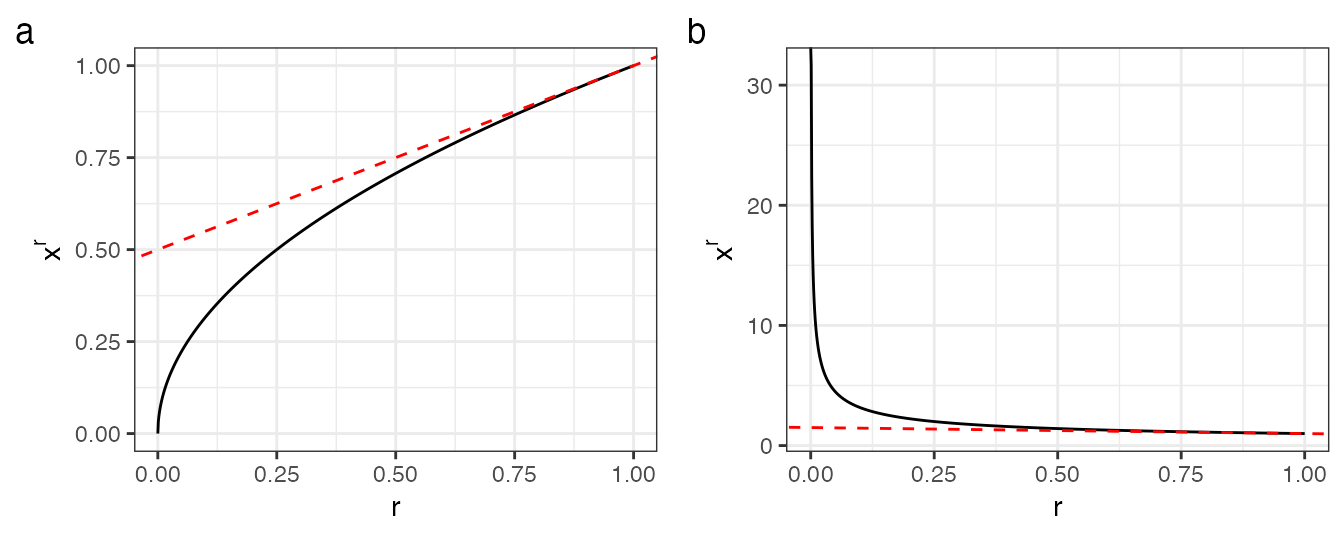
\includegraphics[width=1\linewidth]{MesuresBD_files/figure-latex/LineaireZpsqFig-1} 

}

\caption{Approximation de \({(\mathbf{Zp})}_{s}^{q-1}\) par son développement limité au premier ordre pour (a) \(q=1.5\) (\(r=q-1\)) et (b) \(q=0.5\)}\label{fig:LineaireZpsqFig}
\end{SCfigure}

\normalsize

Le problème majeur de la diversité \(^q\!D^{\mathbf{Z}}\) est qu'elle fournit souvent des valeurs presque indépendantes de \(q\) quand on l'applique à une matrice de similarité fonctionnelle \autocite{Chiu2014b}.
De nombreux exemples, y compris dans l'article original de Leinster et Cobbold, montrent une très faible décroissance de la diversité de \(q=0\) à \(q=2\).
Ce n'est pas un problème théorique mais numérique.
Si la banalité de l'espèce \(s\) est proche de 1, sa puissance \(q\) peut être approchée par son développement limité au premier ordre:
\[{(\mathbf{Zp})}_{s}^{q-1} \approx 1 + (q-1)[{(\mathbf{Zp})}_{s} - 1].\]
Cette approximation linéaire implique que
\[\sum_s{p_s{\left(\mathbf{Zp}\right)}^{q-1}_s} \approx [\sum_s{p_s{\left(\mathbf{Zp}\right)}_s}]^{q-1}.\]
La puissance \(q-1\) disparaît donc dans le calcul de la diversité et l'équation \eqref{eq:Dqz} devient
\[^q\!D^{\mathbf{Z}} \approx \bar{z}\]
où \(\bar{z} = \sum_s{p_s (\mathbf{Zp})_s}\).
Dans les faits, cette approximation vaut pour des valeurs de banalité assez éloignées de 1 (Figure \ref{fig:LineaireZpsqFig}).

Si une majorité des espèces (au sens de la somme de leurs probabilités respectives) a une banalité supérieure à 0,5, l'approximation linéaire est assez bonne et la moyenne généralisée de la banalité est proche de sa moyenne arithmétique.
Ce n'est pas un problème pour la comparaison de profils de diversité de communautés différentes calculés à partir de la même matrice de similarité mais l'interprétation de la diversité en termes de nombres effectifs d'espèces dépendant de \(q\) n'est pas très intuitive.

Le code R nécessaire pour réaliser la figure est:

\scriptsize

\begin{Shaded}
\begin{Highlighting}[]
\NormalTok{r <-}\StringTok{ }\FloatTok{0.5}
\NormalTok{seqZp <-}\StringTok{ }\KeywordTok{seq}\NormalTok{(}\DecValTok{0}\NormalTok{, }\DecValTok{1}\NormalTok{, }\FloatTok{0.001}\NormalTok{)}
\NormalTok{gga <-}\StringTok{ }\KeywordTok{ggplot}\NormalTok{(}\KeywordTok{data.frame}\NormalTok{(}\DataTypeTok{r =}\NormalTok{ seqZp, }\DataTypeTok{xr =}\NormalTok{ seqZp}\OperatorTok{^}\NormalTok{r), }\KeywordTok{aes}\NormalTok{(r, xr)) }\OperatorTok{+}\StringTok{ }
\StringTok{    }\KeywordTok{geom_line}\NormalTok{() }\OperatorTok{+}\StringTok{ }\KeywordTok{geom_abline}\NormalTok{(}\DataTypeTok{intercept =} \DecValTok{1} \OperatorTok{-}\StringTok{ }\NormalTok{r, }\DataTypeTok{slope =}\NormalTok{ r, }\DataTypeTok{col =} \StringTok{"red"}\NormalTok{, }
    \DataTypeTok{lty =} \DecValTok{2}\NormalTok{) }\OperatorTok{+}\StringTok{ }\KeywordTok{labs}\NormalTok{(}\DataTypeTok{y =} \KeywordTok{expression}\NormalTok{(x}\OperatorTok{^}\NormalTok{r)) }\OperatorTok{+}\StringTok{ }\KeywordTok{labs}\NormalTok{(}\DataTypeTok{tag =} \StringTok{"a"}\NormalTok{)}
\NormalTok{r <-}\StringTok{ }\FloatTok{-0.5}
\NormalTok{ggb <-}\StringTok{ }\KeywordTok{ggplot}\NormalTok{(}\KeywordTok{data.frame}\NormalTok{(}\DataTypeTok{r =}\NormalTok{ seqZp, }\DataTypeTok{xr =}\NormalTok{ seqZp}\OperatorTok{^}\NormalTok{r), }\KeywordTok{aes}\NormalTok{(r, xr)) }\OperatorTok{+}\StringTok{ }
\StringTok{    }\KeywordTok{geom_line}\NormalTok{() }\OperatorTok{+}\StringTok{ }\KeywordTok{geom_abline}\NormalTok{(}\DataTypeTok{intercept =} \DecValTok{1} \OperatorTok{-}\StringTok{ }\NormalTok{r, }\DataTypeTok{slope =}\NormalTok{ r, }\DataTypeTok{col =} \StringTok{"red"}\NormalTok{, }
    \DataTypeTok{lty =} \DecValTok{2}\NormalTok{) }\OperatorTok{+}\StringTok{ }\KeywordTok{labs}\NormalTok{(}\DataTypeTok{y =} \KeywordTok{expression}\NormalTok{(x}\OperatorTok{^}\NormalTok{r)) }\OperatorTok{+}\StringTok{ }\KeywordTok{labs}\NormalTok{(}\DataTypeTok{tag =} \StringTok{"b"}\NormalTok{)}
\KeywordTok{grid.arrange}\NormalTok{(gga, ggb, }\DataTypeTok{ncol =} \DecValTok{2}\NormalTok{)}
\end{Highlighting}
\end{Shaded}

\normalsize

La transformation exponentielle négative,
\[z_{s,t} = e^{-u \frac{d_{s,t}}{\max{(d_{s,t})}}},\]
est justifiée par \textcite{Leinster2013}.
\(u\) est une constante positive.
Plus \(u\) est grand, plus la transformation est convexe: les similarités sont tassées vers 0 (figure \ref{fig:EchelleFig}).



\scriptsize

\begin{SCfigure}

{\centering 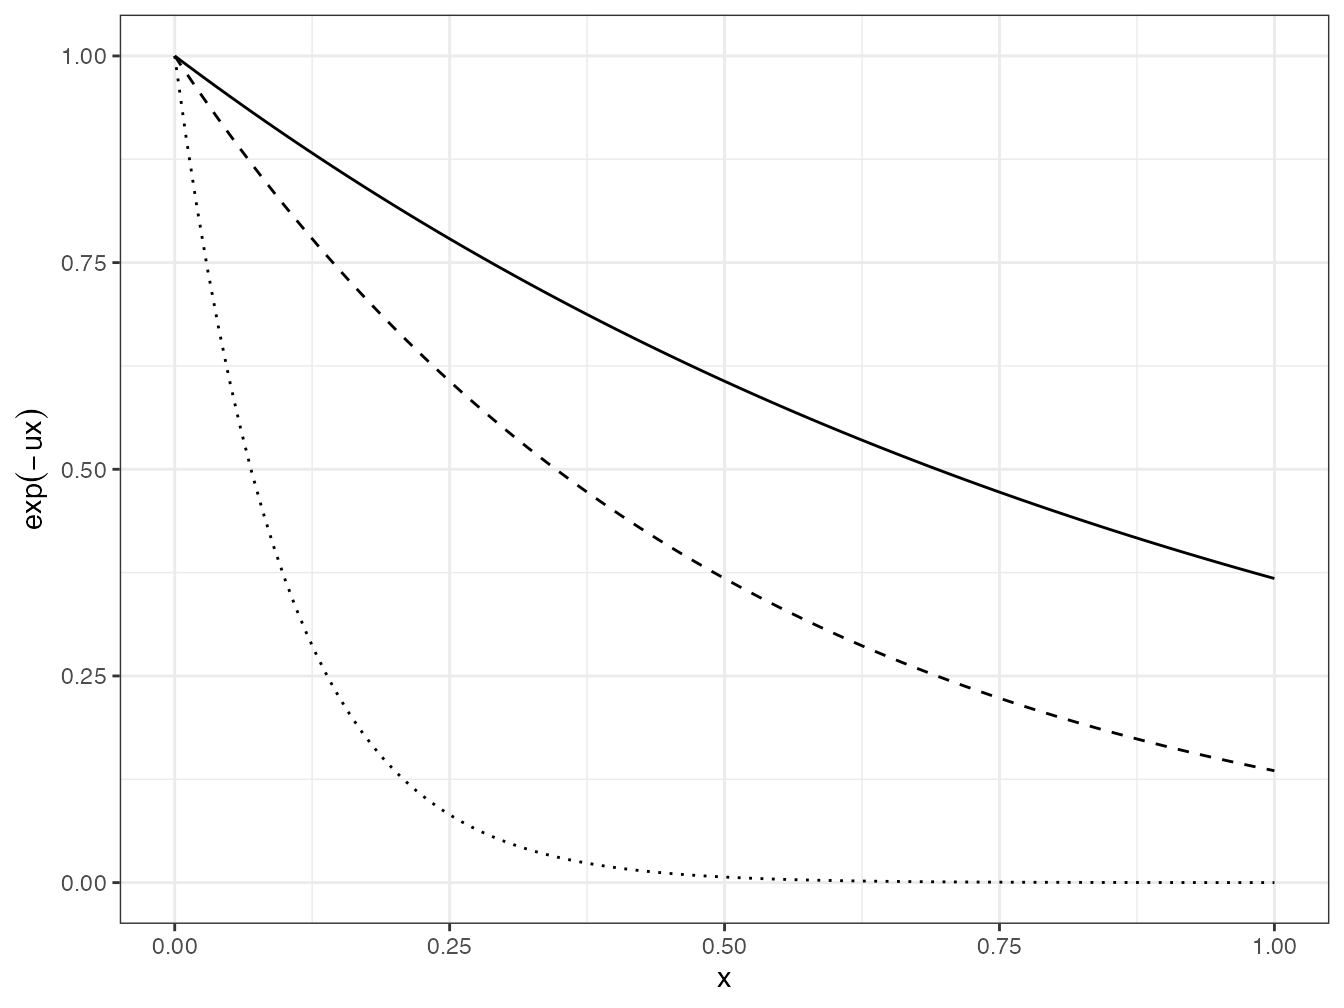
\includegraphics[width=0.8\linewidth]{MesuresBD_files/figure-latex/EchelleFig-1} 

}

\caption{Transformation des distances (en abscisse) en similarités (en ordonnées) selon la valeur de \(u\). Trait plein: \(u=1\); pointillés longs: \(u=2\); pointillés: \(u=10\). Plus \(u\) est grand, plus les similarités sont tassées vers 0.}\label{fig:EchelleFig}
\end{SCfigure}

\normalsize

Le code R nécessaire pour réaliser la figure est:

\scriptsize

\begin{Shaded}
\begin{Highlighting}[]
\KeywordTok{ggplot}\NormalTok{(}\KeywordTok{data.frame}\NormalTok{(}\DataTypeTok{x =} \KeywordTok{seq}\NormalTok{(}\DecValTok{0}\NormalTok{, }\DecValTok{1}\NormalTok{, }\DataTypeTok{by =} \FloatTok{.01}\NormalTok{)), }\KeywordTok{aes}\NormalTok{(x)) }\OperatorTok{+}\StringTok{ }
\StringTok{  }\KeywordTok{stat_function}\NormalTok{(}\DataTypeTok{fun =} \ControlFlowTok{function}\NormalTok{(x) }\KeywordTok{exp}\NormalTok{(}\OperatorTok{-}\NormalTok{x)) }\OperatorTok{+}
\StringTok{  }\KeywordTok{stat_function}\NormalTok{(}\DataTypeTok{fun =} \ControlFlowTok{function}\NormalTok{(x) }\KeywordTok{exp}\NormalTok{(}\OperatorTok{-}\DecValTok{2}\OperatorTok{*}\NormalTok{x), }\DataTypeTok{lty =} \DecValTok{2}\NormalTok{) }\OperatorTok{+}
\StringTok{  }\KeywordTok{stat_function}\NormalTok{(}\DataTypeTok{fun =} \ControlFlowTok{function}\NormalTok{(x) }\KeywordTok{exp}\NormalTok{(}\OperatorTok{-}\DecValTok{10}\OperatorTok{*}\NormalTok{x), }\DataTypeTok{lty =} \DecValTok{3}\NormalTok{) }\OperatorTok{+}
\StringTok{  }\KeywordTok{labs}\NormalTok{(}\DataTypeTok{y =} \KeywordTok{expression}\NormalTok{(}\KeywordTok{exp}\NormalTok{(}\OperatorTok{-}\NormalTok{ux)))}
\end{Highlighting}
\end{Shaded}

\normalsize

Augmenter la valeur de \(u\) diminue les similarités et donc la banalité des espèces, ce qui règle (arbitrairement) le problème de la faible sensibilité de la diversité au paramètre \(q\).

Du point de vue théorique, l'ordre des valeurs de la matrice des distances est justifié (par les différences entre traits fonctionnels par exemple) mais leur distribution ne l'est pas: elle n'est que la conséquence de la méthode de calcul.
Le choix de \(u\) ne change pas l'ordre des distances mais déforme la distribution des similarités.
La distance étant normalisée, \(u\) fixe l'échelle des distances avant la transformation.

Leinster relie la valeur de \(^q\!D^{\mathbf{Z}}\) à la magnitude de l'espace des espèces (espace dans lequel les espèces sont des points dont les distances deux à deux sont décrites par la matrice \(\Delta\), qui doit être euclidienne): la magnitude de l'espace est la valeur maximale que peut atteindre la diversité.
La magnitude est une propriété qui décrit la taille d'un espace dans le cadre de la théorie des catégories.
Modifier \(u\) modifie la magnitude de l'espace selon une relation non triviale: \(u\) est un paramètre au même titre que \(q\).
Quand \(u \to +\infty\), \(\mathbf{Z} \to \mathbf{I}_s\): la diversité tend vers la diversité neutre.
Leinster et Cobbold suggèrent de comparer les profils de diversité en fonction à la fois de \(q\) et de \(u\).

\hypertarget{sec:dqzEstimation}{%
\section{Estimation}\label{sec:dqzEstimation}}

Comme les autres mesures de diversité, \(^q\!D^{\mathbf{Z}}\) est sujette au biais d'estimation.
Deux estimateurs réduisant le biais existent \autocite{Marcon2014e}.
Le premier utilise la technique de \textcite{Chao2003} déjà vue pour la correction du biais de l'entropie de Shannon \eqref{eq:ChaoShen}.
L'estimateur de \(^q\!H^{\mathbf{Z}}\) est

\begin{equation}
  \label{eq:EstHqz}
  ^q\!{\tilde{H}}^{\mathbf{Z}}
  = \sum_s{\frac{\hat{C}\hat{p}_s \ln_q \frac{1}{{\left(\widetilde{\mathbf{Zp}}\right)}_s}}{1-{\left(1-\hat{C}\hat{p}_s\right)}^n}},
\end{equation}

où

\begin{equation}
  \label{eq:EstZp}
  {\left(\widetilde{\mathbf{Zp}}\right)}_s
  = \sum_t{{\hat{C}\hat{p}}_t z_{s,t}} +\left(1-\hat{C}\right)\bar{z}.
\end{equation}

L'estimateur de la diversité est \(^q\!{\tilde{D}}^{\mathbf{Z}} = e^{^q\!{\tilde{H}}^{\mathbf{Z}}}_q\).

L'autre estimateur suppose que la similarité des espèces non observées avec toutes les autres est la similarité moyenne observée.
L'estimation utilise la technique de \textcite{Zhang2014}, qui consiste à développer l'estimateur en série entière au voisinage de \(p_s=1\).
L'estimateur de \(^q\!D^{\mathbf{Z}}\) est, pour \(q\ne 1\),

\begin{equation}
  \label{eq:EstDqz}
  ^q\!{\tilde{D}}^{\mathbf{Z}}
  = {\left\{\hat{K}+\hat{V}
    -\sum_{s\le s_{\ne 0}}{\hat{C}\hat{p}_s{\left[\bar{z}\left(1-\hat{C}\hat{p}_s\right)+\hat{C}\hat{p}_s\right]}^{q-1}}\right\}}
      ^{\frac{1}{1-q}}
\end{equation}

où

\begin{equation}
   \label{eq:EstKDqz}
 \hat{K}=\sum_{s\le s_{\ne 0}}{\hat{C}\hat{p}_s{\left[\left(\sum_{t\le s_{\ne 0}}{\hat{C}\hat{p}_t z_{s,t}}\right)+\left(1-\hat{C}\right)\bar{z}\right]}^{q-1}}
\end{equation}

et

\begin{equation}
  \label{eq:EstVDqz}
  \hat{V}=1+\sum_{s\le s_{\ne 0}}{\frac{n_s}{n}\sum^{n-n_s}_{v=1}{{\left(1-\bar{z}\right)}^v\left[\prod^v_{i=1}{\frac{i-q}{i}}\right]\left[\prod^v_{j=1}{\left(1-\frac{n_s-1}{n-j}\right)}\right]}}.
\end{equation}

L'estimateur de \(^q\!H^{\mathbf{Z}}\) est

\begin{equation}
  \label{eq:EstHqz2}
  ^q\!{\tilde{H}}^{\mathbf{Z}}
  = \frac{\hat{K}+\hat{V}-\sum_{s\le s_{\ne 0}}{\hat{C}\hat{p}_s{\left[\bar{z}\left(1-\hat{C}\hat{p}_s\right)+\hat{C}\hat{p}_s\right]}^{q-1}}-1}{1-q}.
\end{equation}

Pour \(q=1\),

\begin{equation}
  \label{eq:EstH1z2}
  ^1\!{\tilde{H}}^{\mathbf{Z}}
  = \hat{L}+\hat{W}+\sum_{s\le s_{\ne 0}}{\hat{C}\hat{p}_s\ln\left[\bar{z}\left(1-\hat{C}\hat{p}_s\right)+\hat{C}\hat{p}_s\right]},
\end{equation}
\begin{equation}
  ^1\!{\tilde{D}}^{\mathbf{Z}}=e^{^1\!{\tilde{H}}^{\mathbf{Z}}},
\end{equation}

où

\begin{equation}
  \label{eq:EstLHqz2}
  \hat{L}=-\sum_{s\le s_{\ne 0}}{\hat{C}\hat{p}_s \ln\left[\left(\sum_{t\le s_{\ne 0}}{{\hat{C}\hat{p}}_jz_{s,t}}\right)+\left(1-\hat{C}\right)\bar{z}\right]},
\end{equation}
\begin{equation}
  \hat{W}=\sum_{s\le s_{\ne 0}}{\frac{n_s}{n}\sum^{n-n_s}_{v=1}{\frac{{\left(1-\bar{z}\right)}^v}{v}\left[\prod^v_{j=1}{\left(1-\frac{n_s-1}{n-j}\right)}\right]}}.
\end{equation}

Le package \emph{entropart} fournit les fonctions \texttt{Dqz} et \texttt{HqZ} pour calculer ces estimateurs.

\scriptsize

\begin{Shaded}
\begin{Highlighting}[]
\KeywordTok{data}\NormalTok{(Paracou618)}
\CommentTok{# Matrice de distances fonctionnelles}
\NormalTok{DistanceMatrix <-}\StringTok{ }\KeywordTok{as.matrix}\NormalTok{(Paracou618.dist)}
\CommentTok{# Matrice de similarité}
\NormalTok{Z <-}\StringTok{ }\DecValTok{1} \OperatorTok{-}\StringTok{ }\NormalTok{DistanceMatrix}\OperatorTok{/}\KeywordTok{max}\NormalTok{(DistanceMatrix)}
\CommentTok{# Calcul de la diversité}
\KeywordTok{Dqz}\NormalTok{(Paracou618.MC}\OperatorTok{$}\NormalTok{Ns, }\DataTypeTok{q =} \DecValTok{1}\NormalTok{, Z)}
\end{Highlighting}
\end{Shaded}

\begin{verbatim}
##     Best 
## 1.488083
\end{verbatim}

\normalsize

\hypertarget{diversituxe9-phyloguxe9nuxe9tique}{%
\section{Diversité phylogénétique}\label{diversituxe9-phyloguxe9nuxe9tique}}



\scriptsize

\begin{SCfigure}

{\centering \includegraphics[width=0.8\linewidth]{images/ArbreA} 

}

\caption{Arbre phylogénétique ou fonctionnel hypothétique. 5 espèces sont présentes (\(S=5\)), leurs probabilités notées \(p_1\) à \(p_5\). Les noms des branches sont affichés.}\label{fig:ArbreA6}
\end{SCfigure}

\normalsize

La diversité phylogénétique \(^{q}\!\bar{D}(T)\) appliquée à un arbre ultramétrique est un cas particulier de \(^q\!D^{\mathbf{Z}}\) pour une matrice \(\mathbf{Z}\) dont les lignes et colonnes sont la similarité des ``espèces historiques'' \autocite[proposition A7]{Leinster2012}, c'est-à-dire les couples (espèce actuelle; branche ancestrale).



\scriptsize

\begin{table}

\caption{\label{tab:MatricePhylo}Matrice de similarité correspondant à l'arbre phylogénétique en exemple. Les noms des lignes et colonnes sont les couples (espèce actuelle; branche ancestrale).}
\centering
\fontsize{10}{12}\selectfont
\begin{tabu} to \linewidth {>{\raggedright}X>{\raggedleft}X>{\raggedleft}X>{\raggedleft}X>{\raggedleft}X>{\raggedleft}X>{\raggedleft}X>{\raggedleft}X>{\raggedleft}X>{\raggedleft}X>{\raggedleft}X}
\toprule
 & $(1;b_{1,1})$ & $(1;b_{3,1})$ & $(2;b_{1,2})$ & $(2;b_{3,1})$ & $(3;b_{1,3})$ & $(3;b_{2,3})$ & $(4;b_{1,4})$ & $(4;b_{2,3})$ & $(5;b_{1,5})$ & $(5;b_{2,3})$\\
\midrule
$(1;b_{1,1})$ & 1 & 1 & 0 & 0 & 0 & 0 & 0 & 0 & 0 & 0\\
$(1;b_{3,1})$ & 1 & 1 & 1 & 1 & 0 & 0 & 0 & 0 & 0 & 0\\
$(2;b_{1,2})$ & 0 & 0 & 1 & 1 & 0 & 0 & 0 & 0 & 0 & 0\\
$(2;b_{3,1})$ & 1 & 1 & 1 & 1 & 0 & 0 & 0 & 0 & 0 & 0\\
$(3;b_{1,3})$ & 0 & 0 & 0 & 0 & 1 & 1 & 0 & 0 & 0 & 0\\
\addlinespace
$(3;b_{2,3})$ & 0 & 0 & 0 & 0 & 1 & 1 & 1 & 1 & 1 & 1\\
$(4;b_{1,4})$ & 0 & 0 & 0 & 0 & 0 & 0 & 1 & 1 & 0 & 0\\
$(4;b_{2,3})$ & 0 & 0 & 0 & 0 & 1 & 1 & 1 & 1 & 1 & 1\\
$(5;b_{1,5})$ & 0 & 0 & 0 & 0 & 0 & 0 & 0 & 0 & 1 & 1\\
$(5;b_{2,3})$ & 0 & 0 & 0 & 0 & 1 & 1 & 1 & 1 & 1 & 1\\
\bottomrule
\end{tabu}
\end{table}

\normalsize

Par exemple, l'espèce 1 et les branches \(b_{1,1}\) et \(b_{3,1}\) fournissent les deux premières lignes et colonnes de la matrice; l'espèce 5 et les branches \(b_{1,5}\) et \(b_{2,3}\), les deux dernières.

La diversité phylogénétique \(^{q}\!\hat{D}(T)\) est obtenue quand les éléments de la matrice \(\mathbf{Z}\) suivent les règles suivantes: les éléments de toutes les colonnes correspondant à une espèce donnée (par exemple les deux premières colonnes qui correspondent à l'espèce 1) valent 1 pour toutes les lignes correspondant à une branche dont l'espèce descend (les trois lignes correspondant aux branches \(b_{1,1}\) et \(b_{3,1}\)); les éléments dont l'espèce en colonne ne descend pas de la branche en ligne valent 0.
La matrice n'est donc pas symétrique, mais c'est une matrice de similarité dont la diagonale vaut 1.

La probabilité de chaque espèce historique est la somme de celles des espèces actuelles qui en descendent, multipliée par la longueur de la branche normalisée par la hauteur de l'arbre.
Dans l'exemple, la hauteur totale de l'arbre est \(T=T_1 + T_2 + T_3\).
Les probabilités des espèces historiques sont
\[(p_1 \frac{l(b_{1,1})}{T}, (p_1 + p_2) \frac{l(b_{3,1})}{T}, p_2 \frac{l(b_{1,2})}{T}, \dots, (p_3 + p_4 + p_5) \frac{l(b_{2,3})}{T}).\]

Les dimensions de la matrice de similarité et du vecteur de probabilités deviennent rapidement très grandes et leur écriture pénible: il est bien plus simple de calculer la diversité phylogénétique à partir des distances dans l'arbre et des probabilités des espèces.
Cette équivalence de méthodes n'a donc pas d'intérêt pratique mais montre que la diversité de Leinster et Cobbold généralise la diversité phylogénétique.
Cependant, le calcul de \(^q\!{\hat{D}}^{\mathbf{Z}}\) à partir d'une matrice \(\mathbf{Z}\) qui serait la simple transformation des distances de l'arbre phylogénétique, c'est-à-dire 1 moins les distances normalisées par la hauteur de l'arbre, ne donne pas la valeur de la diversité phylogénétique \(^{q}\!\bar{D}(T)\), sauf dans le cas particulier de la diversité de Rao, \(q=2\).

Pour un arbre non ultramétrique, il est possible de définir une matrice \(\mathbf{Z}\) similaire à celle de la table \ref{tab:MatricePhylo}, mais ses valeurs non nulles ne sont pas égales à 1.
Elles sont égales au rapport de \(\bar{T}\), la longueur moyenne des branches pondérée par la fréquence des espèces, sur la longueur de la branche: elles dépendent donc des fréquences des espèces et empêchent par conséquent la comparaison de la diversité entre communautés différentes.

\hypertarget{diversituxe9-individuelle-1}{%
\section{Diversité individuelle}\label{diversituxe9-individuelle-1}}

La diversité \(^q\!D^{\mathbf{Z}}\) et tous ses cas particuliers (phylodiversité et diversité neutre) peuvent être envisagés au niveau individuel plutôt qu'au niveau de l'espèce.

Le calcul de la diversité n'est pas affecté par le remplacement d'une espèce par deux espèces identiques.
La ligne et la colonne de la matrice \(\mathbf{Z}\), correspondant à l'espèce \(s\) sont remplacées par deux lignes et colonnes identiques correspondant aux espèces \(s'\) et \(s''\), dont la similarité avec les autres espèces est la même que celle de l'espèce \(s\) et la similarité entre elles égale à 1, les probabilités vérifiant \(p_s=p_{s'}+p_{s''}\).
L'opération peut être répétée jusqu'à la désagrégation complète de la matrice où chaque ligne correspondrait à un individu et les probabilités seraient égales à \({1}/{N}\).
Il n'y donc pas de différence entre la mesure de la diversité individuelle et celle de la diversité spécifique qui n'est qu'une façon pratique de regrouper des individus ayant la même banalité.
Dit autrement, l'entropie d'une communauté est la somme des entropie de ses espèces, qui n'est que la somme pondérée des entropies individuelles si tous les individus d'une espèce ont la même entropie.

La variabilité intraspécifique peut être traitée par un raisonnement similaire.
L'idée d'intégrer aux mesures de diversité la possibilité que tous les individus d'une espèce ne soient pas semblables émerge dans la littérature \autocite{Pavoine2014b,Chiu2014b}.
Mais si des individus de la même espèce ne sont pas totalement similaires, ils ne peuvent pas être regroupés en prenant pour similarité de l'espèce avec elle-même une valeur unique qui résumerait la similarité entre les individus (au lieu de 1) pour tous les ordres de diversité.

Formellement, si l'espèce \(s\) est composée de deux groupes \(s'\) et \(s''\), la banalité du groupe \(s'\) est
\[{\left(\mathbf{Zp}\right)}_{s'}=\sum_{t \ne s', s''}{p_{t}z_{s',t}} + p_{s'} + p_{s''}z_{s',s''},\]
celle du groupe \(s''\) est
\[{\left(\mathbf{Zp}\right)}_{s''}=\sum_{t \ne s', s''}{p_{t}z_{s'',t}} + p_{s'}z_{s',s''} + p_{s''}.\]
Les similarités avec les autres espèces sont identiques: \(z_{s,t}=z_{s',t}=z_{s'',t}\).
La contribution à la diversité des deux groupes
\[\sum_{s'}{p_{s'}{\left(\mathbf{Zp}\right)}^{q-1}_{s'}}+\sum_{s''}{p_{s''}{\left(\mathbf{Zp}\right)}^{q-1}_{s''}}\]
est remplacée après regroupement par
\[\sum_{s}{p_{s}{\left(\mathbf{Zp}\right)}^{q-1}_{s}}.\]
Puisque \(p_s=p_{s'}+p_{s''}\), le regroupement n'est possible quel que soit \(q\) que si les banalités des deux groupes sont identiques, ce qui interdit toute variabilité intraspécifique: \(z_{s',s''}\) est obligatoirement égal à 1.
La non-linéarité de la moyenne généralisée ne permet pas de définir une matrice de similarité intégrant la variabilité intraspécifique.

Dans le cas de la diversité de Rao (\(q=2\)), on peut chercher la valeur de \(z_{s,s}\), différente de 1, définissant la similarité de l'espèce avec elle même pour prendre en compte sa variabilité.
La résolution de l'équation
\[\sum_{s'}{p_{s'}{\left(\mathbf{Zp}\right)}_{s'}}+\sum_{s''}{p_{s''}{\left(\mathbf{Zp}\right)}_{s''}} = \sum_{s}{p_{s}{\left(\mathbf{Zp}\right)}_{s}}\]
permet de trouver
\[z_{s,s}=1+ \frac{2 p_{s'} p_{s''}(z_{s',s''}-1)}{p_s^2}.\]
Dans le cas le plus simple où \(p_{s'}=p_{s''}\), la similarité intraspécifique est \({(1+z_{s',s''})}/{2}\).
La valeur de \(z_{s,s}\) peut être cherchée pour n'importe quelle valeur de \(q\), mais la résolution de l'équation est en général impossible analytiquement, et \(z_{s,s}\) varie avec \(q\).
Se limiter à \(q=2\) simplifie le problème.

L'exemple suivant considère deux espèces, dont une comprenant deux groupes:

\scriptsize

\begin{Shaded}
\begin{Highlighting}[]
\CommentTok{# Similarité entre les deux groupes}
\NormalTok{zs12 <-}\StringTok{ }\FloatTok{0.9}
\CommentTok{# Probabilités des deux groupes}
\NormalTok{ps1 <-}\StringTok{ }\DecValTok{1}\OperatorTok{/}\DecValTok{5}
\NormalTok{ps2 <-}\StringTok{ }\DecValTok{1}\OperatorTok{/}\DecValTok{5}
\CommentTok{# Matrice de similarité}
\NormalTok{(Z2s <-}\StringTok{ }\KeywordTok{matrix}\NormalTok{(}\KeywordTok{c}\NormalTok{(}\DecValTok{1}\NormalTok{, zs12, }\FloatTok{0.5}\NormalTok{, zs12, }\DecValTok{1}\NormalTok{, }\FloatTok{0.5}\NormalTok{, }\FloatTok{0.5}\NormalTok{, }\FloatTok{0.5}\NormalTok{, }\DecValTok{1}\NormalTok{), }\DataTypeTok{nrow =} \DecValTok{3}\NormalTok{))}
\end{Highlighting}
\end{Shaded}

\begin{verbatim}
##      [,1] [,2] [,3]
## [1,]  1.0  0.9  0.5
## [2,]  0.9  1.0  0.5
## [3,]  0.5  0.5  1.0
\end{verbatim}

\begin{Shaded}
\begin{Highlighting}[]
\CommentTok{# Probabilités}
\NormalTok{(P2s <-}\StringTok{ }\KeywordTok{c}\NormalTok{(ps1, ps2, }\DecValTok{1} \OperatorTok{-}\StringTok{ }\NormalTok{ps1 }\OperatorTok{-}\StringTok{ }\NormalTok{ps2))}
\end{Highlighting}
\end{Shaded}

\begin{verbatim}
## [1] 0.2 0.2 0.6
\end{verbatim}

\begin{Shaded}
\begin{Highlighting}[]
\CommentTok{# Diversité}
\KeywordTok{Dqz}\NormalTok{(P2s, }\DecValTok{2}\NormalTok{, Z2s)}
\end{Highlighting}
\end{Shaded}

\begin{verbatim}
##     None 
## 1.329787
\end{verbatim}

\begin{Shaded}
\begin{Highlighting}[]
\CommentTok{# Similarité intraspécifique après regroupement}
\NormalTok{(zss <-}\StringTok{ }\DecValTok{1} \OperatorTok{+}\StringTok{ }\DecValTok{2} \OperatorTok{*}\StringTok{ }\NormalTok{ps1 }\OperatorTok{*}\StringTok{ }\NormalTok{ps2}\OperatorTok{/}\NormalTok{(ps1 }\OperatorTok{+}\StringTok{ }\NormalTok{ps2)}\OperatorTok{^}\DecValTok{2} \OperatorTok{*}\StringTok{ }\NormalTok{(zs12 }\OperatorTok{-}\StringTok{ }\DecValTok{1}\NormalTok{))}
\end{Highlighting}
\end{Shaded}

\begin{verbatim}
## [1] 0.95
\end{verbatim}

\begin{Shaded}
\begin{Highlighting}[]
\CommentTok{# Matrice de similarité après regroupement}
\NormalTok{(Z1s <-}\StringTok{ }\KeywordTok{matrix}\NormalTok{(}\KeywordTok{c}\NormalTok{(zss, }\FloatTok{0.5}\NormalTok{, }\FloatTok{0.5}\NormalTok{, }\DecValTok{1}\NormalTok{), }\DataTypeTok{nrow =} \DecValTok{2}\NormalTok{))}
\end{Highlighting}
\end{Shaded}

\begin{verbatim}
##      [,1] [,2]
## [1,] 0.95  0.5
## [2,] 0.50  1.0
\end{verbatim}

\begin{Shaded}
\begin{Highlighting}[]
\CommentTok{# Probabilité après regroupement}
\NormalTok{(P1s <-}\StringTok{ }\KeywordTok{c}\NormalTok{(ps1 }\OperatorTok{+}\StringTok{ }\NormalTok{ps2, }\DecValTok{1} \OperatorTok{-}\StringTok{ }\NormalTok{ps1 }\OperatorTok{-}\StringTok{ }\NormalTok{ps2))}
\end{Highlighting}
\end{Shaded}

\begin{verbatim}
## [1] 0.4 0.6
\end{verbatim}

\begin{Shaded}
\begin{Highlighting}[]
\CommentTok{# Diversité}
\KeywordTok{Dqz}\NormalTok{(P1s, }\DecValTok{2}\NormalTok{, Z1s)}
\end{Highlighting}
\end{Shaded}

\begin{verbatim}
##     None 
## 1.329787
\end{verbatim}

\normalsize

En pratique, si les similarités entre individus ou groupes sont connues, le regroupement n'a aucun intérêt.
Mais en absence de données individuelles, il est possible de choisir arbitrairement une similarité intraspécifique différente de 1 (ou de façon équivalente une distance différente de 0) pour calculer une diversité d'ordre fixé, de préférence 2.

\hypertarget{diversituxe9-des-valeurs-propres}{%
\section{Diversité des valeurs propres}\label{diversituxe9-des-valeurs-propres}}

L'approche de \textcite{Pavoine2014} permet de prendre en compte la variabilité intraspécifique de façon rigoureuse.
Pour mesurer la diversité neutre, les espèces sont placées dans un espace multidimensionnel, de dimension \(S\).
Chaque espèce est représentée par un vecteur de longueur \(p_s\) sur son axe.
Cette représentation a été utilisée par \textcite{Campos2009} qui ont relié la diversité de Simpson au volume de la sphère sur laquelle se trouve le point définissant la communauté (figure \ref{fig:Campos2009}).



\scriptsize

\begin{SCfigure}

{\centering \includegraphics[width=0.5\linewidth]{images/Campos2009} 

}

\caption{Représentation d'une communauté dans un espace multidimensionnel dont chaque axe correspond à une espèce. La communauté est composée de trois espèces. Le point représentant la communauté se trouve sur la sphère de rayon \(r=\sqrt{\sum_s{p_s^2}}\). Le plan (qui est en réalité un hyperplan de dimension \(S-1\)) d'équation \(\sum_s{p_s}=1\) est représenté par un triangle.}\label{fig:Campos2009}
\end{SCfigure}

\normalsize

La matrice de similarité entre les espèces \(\mathbf{Z}\) permet d'affiner la représentation.
Soit la matrice \(\mathbf{C}=\sqrt{\mathbf{Z}}\).
Chaque espèce \(s\) est maintenant représentée par le vecteur dont la coordonnée sur l'axe \(t\) est \(\sqrt{p_s p_t}c_{s,t}\).
Les axes correspondent aux espèces ``pures'', totalement dissimilaires, les vecteurs des espèces réelles prennent en compte la similarité.
Dans le cas extrême de la diversité neutre, \(\mathbf{C}=\mathbf{I}\), chaque espèce est située uniquement sur son axe.
Dans l'autre cas extrême de totale similarité, où \(\mathbf{C}\) ne contient que des 1, toutes les espèces sont colinéaires.

Il est possible de calculer les \(S\) valeurs propres notées \(\lambda_s\) de la matrice des coordonnées des espèces et de les normaliser: \(\mu_s={\lambda_s}/{\sum_s{\lambda_s}}\).
La communauté peut maintenant être représentée par ses valeurs propres \(\mu_s\) correspondant à la proportion d'une ``espèce composite'' pure sur chaque axe généré par les vecteurs propres: cette transformation est une ACP non centrée, non réduite.
La diversité HCDT des valeurs propres est la diversité de la communauté, qui sera notée ici \(^q\!D^{\mathbf{Z}}(\Lambda)\).

La définition de cette diversité autorise toute matrice \(\mathbf{C}\) symétrique, dont les valeurs de similarité sont positives ou nulles, strictement positives sur la diagonale.
Si \(\mathbf{C}\) est la racine carrée d'une matrice de similarité au sens strict \(\mathbf{Z}\), c'est-à-dire contenant des valeurs comprises entre 0 et 1 et dont les éléments de la diagonale sont tous égaux à 1, alors \(^2\!D^{\mathbf{Z}}(\Lambda)\) est égale à la diversité de Rao appliquée à une matrice de distances \(\mathbf{D}=1-\mathbf{Z}\).
La définition de \(\mathbf{C}\) comme racine carrée de \(\mathbf{Z}\) se justifie par des raisons géométriques: la norme de chaque vecteur représentant une espèce est la racine carrée de la somme des carrés de ses coordonnées.
Le carré de la norme du vecteur de l'espèce \(s\) est donc \(p_s\) multiplié par la banalité de l'espèce.

Si \(\mathbf{Z}=\mathbf{I}_s\), l'ACP ne modifie pas le nuage de points original et \(^q\!D^{\mathbf{Z}}(\Lambda)={^{q}\!D}\).

L'exemple suivant calcule la diversité de la méta-communauté \texttt{Paracou618} selon la matrice de distances \texttt{Paracou618.dist}.

\scriptsize

\begin{Shaded}
\begin{Highlighting}[]
\CommentTok{# Probabilités}
\NormalTok{Ps <-}\StringTok{ }\NormalTok{Paracou618.MC}\OperatorTok{$}\NormalTok{Ps[Paracou618.MC}\OperatorTok{$}\NormalTok{Ps }\OperatorTok{>}\StringTok{ }\DecValTok{0}\NormalTok{]}
\CommentTok{# Matrice de distances fonctionnelles}
\NormalTok{DistanceMatrix <-}\StringTok{ }\KeywordTok{as.matrix}\NormalTok{(Paracou618.dist)}
\CommentTok{# Mise en correspondance de la matrice et du vecteur de}
\CommentTok{# probabilités}
\NormalTok{D <-}\StringTok{ }\NormalTok{DistanceMatrix[}\KeywordTok{names}\NormalTok{(Ps), }\KeywordTok{names}\NormalTok{(Ps)]}
\CommentTok{# Normalisation}
\NormalTok{D <-}\StringTok{ }\NormalTok{D}\OperatorTok{/}\KeywordTok{max}\NormalTok{(D)}
\CommentTok{# Transformation en matrice de similarité}
\NormalTok{Z <-}\StringTok{ }\DecValTok{1} \OperatorTok{-}\StringTok{ }\NormalTok{D}
\CommentTok{# Matrice diagonale contenant les probabilités}
\NormalTok{Q <-}\StringTok{ }\KeywordTok{diag}\NormalTok{(Ps)}
\CommentTok{# Matrice des espèces (les lignes de Sp sont les coordonnées}
\CommentTok{# des vecteurs)}
\NormalTok{Sp <-}\StringTok{ }\KeywordTok{sqrt}\NormalTok{(Q) }\OperatorTok\StringTok{ }\KeywordTok{sqrt}\NormalTok{(Z) }\OperatorTok\StringTok{ }\KeywordTok{sqrt}\NormalTok{(Q)}
\CommentTok{# Valeurs propres normalisées}
\NormalTok{Lambda <-}\StringTok{ }\KeywordTok{svd}\NormalTok{(Sp)}\OperatorTok{$}\NormalTok{d}
\NormalTok{Mu <-}\StringTok{ }\NormalTok{Lambda}\OperatorTok{/}\KeywordTok{sum}\NormalTok{(Lambda)}
\CommentTok{# Comparaison des valeurs à q=2}
\KeywordTok{Diversity}\NormalTok{(Mu, }\DecValTok{2}\NormalTok{)}
\end{Highlighting}
\end{Shaded}

\begin{verbatim}
##     None 
## 1.540061
\end{verbatim}

\begin{Shaded}
\begin{Highlighting}[]
\CommentTok{# Diversité de Rao}
\KeywordTok{Dqz}\NormalTok{(Ps, }\DecValTok{2}\NormalTok{, Z)}
\end{Highlighting}
\end{Shaded}

\begin{verbatim}
##     None 
## 1.490786
\end{verbatim}

\begin{Shaded}
\begin{Highlighting}[]
\CommentTok{# La valeur à q=0 est le nombre d'espèces}
\KeywordTok{Diversity}\NormalTok{(Mu, }\DecValTok{0}\NormalTok{)}
\end{Highlighting}
\end{Shaded}

\begin{verbatim}
## None 
##  229
\end{verbatim}

\begin{Shaded}
\begin{Highlighting}[]
\KeywordTok{length}\NormalTok{(Ps)}
\end{Highlighting}
\end{Shaded}

\begin{verbatim}
## [1] 229
\end{verbatim}

\normalsize

La valeur de la diversité des valeurs propres est différente de celle de la diversité de Rao à cause des approximations numériques liées au calcul des valeurs propres (qui nécessitent l'inversion d'une matrice carrée de dimension \(S\)).
La valeur exacte est celle donnée par \texttt{Dqz()}.

Le profil de diversité se trouve en figure \ref{fig:DqZLambdaFig}.



\scriptsize

\begin{SCfigure}

{\centering \includegraphics[width=0.8\linewidth]{MesuresBD_files/figure-latex/DqZLambdaFig-1} 

}

\caption{Profil de diversité des valeurs propres de la méta-communauté \texttt{Paracou618}.}\label{fig:DqZLambdaFig}
\end{SCfigure}

\normalsize

Code R pour la figure:

\scriptsize

\begin{Shaded}
\begin{Highlighting}[]
\NormalTok{DqZLambda <-}\StringTok{ }\KeywordTok{CommunityProfile}\NormalTok{(Diversity, Mu)}
\NormalTok{Xlab <-}\StringTok{ "Ordre de diversité"}
\NormalTok{Ylab <-}\StringTok{ "Diversité"}
\KeywordTok{autoplot}\NormalTok{(DqZLambda, }\DataTypeTok{xlab =}\NormalTok{ Xlab, }\DataTypeTok{ylab =}\NormalTok{ Ylab) }\OperatorTok{+}\StringTok{ }\KeywordTok{scale_y_log10}\NormalTok{()}
\end{Highlighting}
\end{Shaded}

\normalsize

La diversité des valeurs propres permet de ramener le problème de la diversité d'espèces partiellement similaires au calcul de la diversité neutre d'une communauté d'espèces composites totalement dissimilaires.

Les éléments de la diagonale de la matrice de similarité ne sont pas forcément égaux à 1: des valeurs inférieures correspondent à la variabilité intraspécifique, selon le mécanisme de regroupement traité au paragraphe précédent.
Les raisons qui empêchent d'utiliser des valeurs de similarité intraspécifique différentes de 1 dans le calcul de la diversité de Leinster et Cobbold ne s'appliquent pas ici: quelle que soit la valeur de \(q\), les valeurs propres sont les mêmes.

Les limites de la diversité des valeurs propres sont cependant nombreuses.
La première est numérique: son calcul est imprécis dans des communautés très riches.
L'inversion d'une matrice de dimension 200 ou plus est toujours problématique.

Les espèces non échantillonnées entraînent un biais d'estimation: le nombre de dimensions est sous-estimé.
Comme les espèces manquantes ont une faible probabilité, leur vecteur est petit et n'influe pas beaucoup sur la diagonalisation de la matrice.
Les valeurs propres manquantes sont donc petites.
Elles influent sur la diversité pour les faibles valeurs de \(q\), notamment la diversité d'ordre 0 qui est le nombre de dimensions de la matrice des espèces (en général, le nombre d'espèces, ou une valeur inférieure si des espèces sont colinéaires).
Il n'existe pas de technique pour corriger ce biais d'estimation.

La composition de la communauté en espèces composites dépend à la fois de la matrice de similarité et des probabilités des espèces réelles.
Elle est donc unique pour chaque communauté, ce qui empêche toute décomposition de la diversité selon les méthodes présentées plus loin.

\hypertarget{sec:dqzSynthese}{%
\section{Synthèse}\label{sec:dqzSynthese}}

\(^{q}\!D(T)\) est l'exponentielle d'ordre \(q\) de la moyenne pondérée de l'entropie HCDT calculée à chaque période de l'arbre phylogénétique.

\(^q\!D^{\mathbf{Z}}\) est l'exponentielle d'ordre \(q\) de l'entropie de Ricotta et Szeidl, mais aussi l'inverse de la banalité moyenne des espèces de la communauté.

\(^q\!D^{\mathbf{Z}}\) et \(^{q}\!D\) sont des nombres effectifs d'espèces, respectent toutes les propriétés demandées à une mesure de diversité dont le principe de réplication.
Leurs valeurs sont identiques pour \(q=2\) (diversité de Rao).
\(^q\!D^{\mathbf{Z}}\) est moins sensible au paramètre \(q\) que \(^{q}\!D(T)\): la figure \ref{fig:ComparaisonDqFig} compare les deux mesures.

Le rôle du paramètre est assez différent: dans \(^q\!D^{\mathbf{Z}}\), la banalité des espèces est à la puissance \(q\) alors que leur probabilité est à la puissance 1.
Le paramètre détermine l'importance donnée aux espèces \emph{originales}, c'est-à-dire dont la banalité est petite, et non aux espèces \emph{rares}.
Les deux notions se confondent quand la diversité neutre est considérée: la banalité d'une espèce se réduit alors à sa fréquence.



\scriptsize

\begin{SCfigure}

{\centering \includegraphics[width=0.8\linewidth]{MesuresBD_files/figure-latex/ComparaisonDqFig-1} 

}

\caption{Diversité phylogénétique (l'arbre est une taxonomie) d'ordre \(q\) de deux hectares de forêt de Paracou: \(^q\!D^{\mathbf{Z}}\) (trait plein) et \(^{q}\!\hat{D}(T)\) (pointillé).}\label{fig:ComparaisonDqFig}
\end{SCfigure}

\normalsize

Le code R nécessaire pour réaliser la figure est:

\scriptsize

\begin{Shaded}
\begin{Highlighting}[]
\NormalTok{q <-}\StringTok{ }\KeywordTok{c}\NormalTok{(}\KeywordTok{seq}\NormalTok{(}\DecValTok{0}\NormalTok{, }\DecValTok{3}\NormalTok{, }\FloatTok{0.1}\NormalTok{))}
\CommentTok{# Réutilisation de Paracou618.Taxonomy au format phylog (cf.}
\CommentTok{# calcul de FAD)}
\NormalTok{DistanceMatrix <-}\StringTok{ }\KeywordTok{as.matrix}\NormalTok{(Tree}\OperatorTok{$}\NormalTok{Wdist}\OperatorTok{^}\DecValTok{2}\OperatorTok{/}\DecValTok{2}\NormalTok{)}
\NormalTok{Z <-}\StringTok{ }\DecValTok{1} \OperatorTok{-}\StringTok{ }\NormalTok{DistanceMatrix}\OperatorTok{/}\KeywordTok{max}\NormalTok{(DistanceMatrix)}
\NormalTok{Divqz <-}\StringTok{ }\KeywordTok{sapply}\NormalTok{(q, }\ControlFlowTok{function}\NormalTok{(q) }\KeywordTok{Dqz}\NormalTok{(Paracou618.MC}\OperatorTok{$}\NormalTok{Ps, q, Z))}
\NormalTok{Divq <-}\StringTok{ }\KeywordTok{sapply}\NormalTok{(q, }\ControlFlowTok{function}\NormalTok{(q) }\KeywordTok{ChaoPD}\NormalTok{(Paracou618.MC}\OperatorTok{$}\NormalTok{Ps, }\DataTypeTok{q =}\NormalTok{ q, }
    \DataTypeTok{PhyloTree =}\NormalTok{ Paracou618.Taxonomy))}
\KeywordTok{ggplot}\NormalTok{(}\KeywordTok{data.frame}\NormalTok{(q, Divq, Divqz), }\KeywordTok{aes}\NormalTok{(q)) }\OperatorTok{+}\StringTok{ }\KeywordTok{geom_line}\NormalTok{(}\KeywordTok{aes}\NormalTok{(}\DataTypeTok{y =}\NormalTok{ Divqz)) }\OperatorTok{+}\StringTok{ }
\StringTok{    }\KeywordTok{geom_line}\NormalTok{(}\KeywordTok{aes}\NormalTok{(}\DataTypeTok{y =}\NormalTok{ Divq), }\DataTypeTok{lty =} \DecValTok{2}\NormalTok{) }\OperatorTok{+}\StringTok{ }\KeywordTok{labs}\NormalTok{(}\DataTypeTok{y =} \StringTok{"Diversité"}\NormalTok{)}
\end{Highlighting}
\end{Shaded}

\normalsize

\(^q\!D^{\mathbf{Z}}\) est particulièrement intéressante pour mesurer la diversité fonctionnelle, souvent définie à partir d'une matrice de distances entre les espèces.
La transformation d'une matrice en un arbre phylogénétique déforme les données \autocite{Pavoine2005a,Podani2006,Podani2007}.
La diversité de Leinster et Cobbold est calculée directement à partir de la matrice.

Si l'arbre phylogénétique n'est pas ultramétrique, le calcul de la diversité est possible, mais la matrice \(\mathbf{Z}\) contient alors des valeurs comprises entre 0 et 1 qui dépendent des effectifs des espèces actuelles (ils interviennent dans le calcul de la hauteur de l'arbre qui est la moyenne de la longueur des branches).
La dépendance entre similarité et fréquence des espèces constitue un problème théorique qui empêche d'interpréter la diversité calculée à partir d'un arbre non ultramétrique.

Enfin, il est possible de désagréger les données jusqu'au niveau individuel si la distance entre paires d'individus est connue.
En revanche, la prise en compte de la variabilité intraspécifique par une similarité intraspécifique inférieure à 1 n'est possible que pour un ordre de diversité fixé: il n'est pas possible d'obtenir un profil de diversité de cette façon.

\hypertarget{part-diversituxe9-beta-et-duxe9composition}{%
\part{Diversité beta et décomposition}\label{part-diversituxe9-beta-et-duxe9composition}}

\hypertarget{sec:betaCadre}{%
\chapter{Cadre}\label{sec:betaCadre}}

\scriptsize

\normalsize

\scriptsize

\begin{Essentiel}
La diversité \(\beta\) désigne la différentiation entre communautés,
c'est-à-dire une mesure de divergence de composition spécifique entre
elle, ou bien la divergence entre elles et leur assemblage, appelée
diversité proportionnelle. La conciliation de ces deux définitions fait
toujours l'objet de recherches.
\end{Essentiel}

\normalsize

La notion de diversité \(\beta\) a été introduite par \textcite{Whittaker1960}, page 320, comme le niveau de changement dans la composition des communautés, ou le degré de différenciation des communautés, en relation avec les changements de milieu.
La traduction de cette notion intuitive en une définition sans ambiguïté est encore une question de recherche et de débats.

\textcite{Anderson2011} fournissent une revue des analyses utiles de la diversité \(\beta\) en forme de guide à destination des écologues reprise ici en introduction.
La distinction entre diversité de différenciation et diversité proportionnelle est présentée ensuite.

Pour simplifier l'exposé, les individus seront échantillonnés dans des communautés, appartenant à une méta-communauté.
Le tableau \ref{tab:Notations} résume les notations.

Des exemples montrent comment calculer cette diversité, principalement à l'aide du package \emph{entropart}.
Le package contient les données d'inventaire de deux hectares du dispositif de Paracou.
Les données sont organisées dans le package sous la forme d'un objet \texttt{MetaCommunity} qui contient notamment la matrice des \(n_{s,i}\).
Les parcelles de Paracou sont dans l'objet \texttt{Paracou618.MC}.

\scriptsize

\begin{Shaded}
\begin{Highlighting}[]
\KeywordTok{library}\NormalTok{(entropart)}
\KeywordTok{summary}\NormalTok{(Paracou618.MC)}
\end{Highlighting}
\end{Shaded}

\begin{verbatim}
## Meta-community (class 'MetaCommunity') made of 1124 individuals in 2 
## communities and 425 species. 
## 
## Its sample coverage is 0.92266748426447 
## 
## Community weights are: 
## [1] 0.5720641 0.4279359
## Community sample numbers of individuals are: 
## P006 P018 
##  643  481 
## Community sample coverages are: 
##      P006      P018 
## 0.8943859 0.8463782
\end{verbatim}

\normalsize



\scriptsize

\begin{table}

\caption{\label{tab:Notations}Notations des effectifs, tableau espèces-communautés.}
\centering
\fontsize{9}{11}\selectfont
\begin{tabu} to \linewidth {>{\raggedright}X>{\raggedright}X>{\raggedright}X}
\toprule
 & Communauté $i$ & $\dots$ Total: méta-communauté\\
\midrule
Espèce $s$ & $n_{s,i}$: nombre d'individus de l'espèce $s$ dans la communauté $i$. $\hat{p}_{s|i}=n_{s,i}/n_{+i}$ est l'estimateur de la probabilité $p_{s|i}$ qu'un individu de la communauté $i$ soit de l'espèce $s$. & $n_{s+}=\sum_i{n_{s,i}}$. $p_s=\sum_i{w_{i}p_{s|i}}$\\
$\dots$ &  & \\
Total & $n_{s+}=\sum_i{n_{s,i}}$. $p_s=\sum_i{w_{i}p_{s|i}}$ & $n$: nombre total d'individus échantillonnés\\
\bottomrule
\end{tabu}
\end{table}

\normalsize

\hypertarget{duxe9finition-de-la-diversituxe9-beta-par-objectifs}{%
\section{\texorpdfstring{Définition de la diversité \(\beta\) par objectifs}{Définition de la diversité \textbackslash beta par objectifs}}\label{duxe9finition-de-la-diversituxe9-beta-par-objectifs}}

\textcite{Anderson2011} proposent une revue des définitions de la diversité \(\beta\) selon les analyses écologiques auxquelles elles peuvent contribuer plutôt que selon leurs propriétés mathématiques.

Deux types de diversité \(\beta\) peuvent être définies \autocite{Vellend2001} en accord avec les notions originales de Whittaker: le \emph{remplacement} (\emph{turnover}) des espèces le long d'un gradient environnemental, spatial ou temporel et la \emph{variation} de la composition spécifique entre communautés, qui diffèrent de la méta-communauté et entre elles.
Ces deux définitions sont présentées sur les figures \ref{fig:Anderson2011a} et \ref{fig:Anderson2011b} \autocite{Anderson2011}.



\scriptsize

\begin{SCfigure}

{\centering \includegraphics[width=0.8\linewidth]{images/Anderson2011a} 

}

\caption{Diversité \(\beta\) liée au remplacement des espèces le long d'un gradient. \(\Delta{y}\) est la mesure de la dissimilarité entre deux communautés. \(\mathbf{x}\) est un gradient environnemental, spatial ou temporel. \(\Delta{x}\) est l'écart entre deux points du gradient.}\label{fig:Anderson2011a}
\end{SCfigure}

\normalsize



\scriptsize

\begin{SCfigure}

{\centering \includegraphics[width=0.8\linewidth]{images/Anderson2011b} 

}

\caption{Diversité \(\beta\) liée à la variation de la composition spécifique. \(\beta_W\) est le rapport entre la diversité \(\gamma\) et la diversité \(\alpha\), \(\beta_{Add}\) leur différence. \(d_{ij}\) est la dissimilarité entre les communautés \(i\) et \(j\). \(\hat{\sigma}^2\) est la variance de cette dissimilarité, \(\bar{d}\) sa moyenne. Si \(d\) est une distance euclidienne, \(\bar{d}_{cen}\) est la distance moyenne des communautés à leur centre de gravité.}\label{fig:Anderson2011b}
\end{SCfigure}

\normalsize

Les mesures de remplacement ne sont pas traitées en détail dans ce chapitre mais simplement présentées ici.

La plus simple (figure \ref{fig:Anderson2011a}, T1) est la dissimilarité entre deux communautés notée \(\Delta{y}\).
De nombreuses mesures de dissimilarité existent, elles sont détaillées dans le chapitre \ref{chap:BetaPaires}.
Whittaker n'envisageait que la présence ou l'absence des espèces, mais leur abondance peut être prise en compte.

Cette dissimilarité peut être analysée en fonction du gradient de référence.
La dissimilarité entre des paires de communautés présentant la même différence (par exemple ayant subi ou non un traitement) situées le long d'un gradient (par exemple la fertilité du sol) peut être analysée en fonction de ce gradient (figure \ref{fig:Anderson2011a}, T2).
Plus classiquement, la diversité \(\beta\) peut être régressée contre la valeur du gradient (T3).
La dissimilarité de chaque paire de communautés est confrontée à son écart sur le gradient.
Les deux analyses précédentes peuvent être combinées pour mesurer le remplacement des espèces selon deux gradients emboîtés (T6).

Une variation sur le modèle T2 consiste à le représenter sous la forme d'un modèle de décroissance en fonction de la distance \autocite{Nekola1999}, éventuellement pour plusieurs groupes de communautés (figure \ref{fig:Anderson2011a}, T4 et T5).
L'indice de Simpson spatialement explicite (Section \ref{sec:SimpsonSpatial}) entre dans ce cadre bien qu'il soit construit différemment.

Les mesures de variation (figure \ref{fig:Anderson2011b}, V1) concernent la dissimilarité entre plusieurs communautés ou entre chaque communauté et la méta-communauté.
L'équivalence de ces deux concepts n'est pas évidente: elle a été montrée pour les mesures de dissimilarité entre paires de communautés par \textcite{Legendre1999}; \textcite{Legendre2001}; \textcite{Legendre2005} et pour l'entropie de Rao par \textcite{Pavoine2004} mais reste une question ouverte pour l'entropie HCDT en général.

La diversité \(\beta\) peut être mesurée pour un assemblage de communautés au choix comme la moyenne des dissimilarités entre les paires de communautés ou à partir des diversités \(\gamma\) et \(\alpha\), c'est-à-dire en tant que mesure dérivée.
Cette dernière approche est traitée dans ce chapitre, où il sera montré que la mesure dérivée est aussi une dissimilarité moyenne entre communautés et méta-communauté.

Si la diversité est mesurée comme moyenne des dissimilarités, elle peut être analysée par des méthodes d'ordination indirectes (figure \ref{fig:Anderson2011b}, V2) ou directes (V3). Elle peut aussi être comparée entre méta-communautés ou modélisée en fonction d'un gradient environnemental (V4), de façon similaire au modèle T6.

La diversité \(\beta\) peut être décomposée en niveaux hiérarchiques emboîtés (V5). Des tests statistiques sont nécessaires pour comparer les niveaux: par exemple, montrer que la diversité (inter) entre des communautés supposées différentes est significativement plus grande que celle (intra) des placettes d'échantillonnage de chacune d'entre elles, à la manière d'une analyse de variance (V6).
D'autres analyses sont bien sûr envisageables, comme la comparaison de la forme de la courbe de dissimilarité moyenne entre paires de communautés en fonction de la distance à des patrons connus, issus de simulation de processus à identifier \autocite{Rejou-Mechain2011}.

\hypertarget{sec:betaTypo}{%
\section{Typologie des mesures}\label{sec:betaTypo}}

Cette approche utilitaire est complétée par le cadre théorique de \textcite{Jurasinski2009} qui distinguent plusieurs types de mesures de diversité:

\begin{itemize}
\tightlist
\item
  La diversité d'inventaire (\emph{inventory diversity}), qui traite des données récoltées sur une unité spatiale, ce qui correspond à la définition des diversités\(\ \alpha\) et \(\gamma\);
\item
  La diversité de différenciation (\emph{differentiation diversity}), qui mesure à quel point les unités spatiales sont différentes, ce qui correspond à la définition littérale de la diversité \(\beta\) de Whittaker;
\item
  La diversité proportionnelle (\emph{proportional diversity}), diversité \(\beta\) qui se construit par différence ou rapport des diversités \(\gamma\) et \(\alpha\). \textcite{Marcon2014a} ont montré qu'avec une décomposition appropriée de la diversité, la diversité proportionnelle est aussi la divergence entre la distribution des communautés locales et celle de la méta-communauté: la diversité \(\beta\) mesure alors à quel point les unités spatiales sont différentes de leur assemblage plutôt qu'entre elles.
\end{itemize}

Dans son article fondateur, \textcite{Whittaker1960} définit la diversité \(\beta\) comme le niveau de changement dans la composition des communautés, la nomme ``diversité secondaire'' et lui attribue la lettre \(\beta\) en référence à la diversité ``primaire'' mesurable par l'indice \(\alpha\) de Fisher \autocite{Fisher1943}, voir le chapitre \ref{chap:Fisher}.
Il illustre cette définition par une mesure de différentiation: l'indice de Jaccard, mais utilise ensuite une mesure proportionnelle: le rapport des indice \(\alpha\) de l'assemblage des communautés à sa moyenne sur les communautés.
La conciliation des deux approches n'est pas simple.
\textcite{Gregorius2016} montre notamment que les mesures habituelles de diversité proportionnelle ne rendent pas compte correctement de la différentiation.

\hypertarget{sec:betaDecomposition}{%
\section{Décomposition de la diversité}\label{sec:betaDecomposition}}

La façon de décomposer la diversité, aboutissant donc à une diversité \(\beta\) proportionnelle, ne fait pas consensus.
Les éléments du débat sont présentés ici.

\hypertarget{duxe9finitions-de-la-diversituxe9-beta-mesure-duxe9rivuxe9e}{%
\subsection{\texorpdfstring{Définitions de la diversité \(\beta\), mesure dérivée}{Définitions de la diversité \textbackslash beta, mesure dérivée}}\label{duxe9finitions-de-la-diversituxe9-beta-mesure-duxe9rivuxe9e}}

\textcite{Tuomisto2010a} passe en revue l'ensemble des définitions de la diversité \(\beta\) dérivée des diversités \(\gamma\) et \(\alpha\).
Toutes ont en commun:

\begin{itemize}
\tightlist
\item
  Une définition de la mesure de diversité, appliquée à la diversité \(\gamma\), qui est généralement une des mesures vues dans le chapitre \ref{chap:MesuresNeutres};
\item
  Une définition de la diversité \(\alpha\), qui peut être par exemple:

  \begin{itemize}
  \tightlist
  \item
    La diversité locale mesurée dans chaque communauté, indépendamment de toute référence hors de la communauté;
  \item
    De façon équivalente, le nombre d'espèces effectives dans les communautés.
  \item
    Une façon de combiner les diversités \(\gamma\) et \(\alpha\) pour obtenir la diversité \(\beta\), par exemple:

    \begin{itemize}
    \tightlist
    \item
      \(\beta={\gamma}/{\alpha}\);
    \item
      \(\beta=\gamma-\alpha\).
    \end{itemize}
  \end{itemize}
\end{itemize}

L'utilisation des nombres de Hill, la mesure locale de la diversité \(\alpha\) et la définition de la diversité \(\beta\) comme rapport des diversités \(\gamma\) et \(\alpha\) permet de définir la ``vraie diversité'' \autocite{Jost2006,Jost2007} \(\beta\) qui est un nombre de communautés équivalentes (\emph{compositionnal units}) similaire au nombre d'espèces équivalentes des diversités \(\alpha\) et \(\gamma\).
\textcite{Tuomisto2011} milite pour que le terme diversité soit réservé à la vraie diversité (homogène à un nombre d'espèces) et que les autres mesures soient appelées différemment: ``entropie'' de Shannon ou ``probabilité'' de Gini-Simpson notamment.

\hypertarget{sec:DebatDecomposition}{%
\subsection{Le débat sur la décomposition}\label{sec:DebatDecomposition}}

L'objectif est de décomposer la diversité totale, notée \(\gamma\) en une composante inter-groupes, notée \(\beta\) et une composante intra-groupes notée \(\alpha\).

Whittaker \autocite*{Whittaker1960,Whittaker1972} est l'auteur de ce concept.
Il a posé le principe que la diversité \(\gamma\) devait être le produit des diversités \(\alpha\) et \(\beta\).

\textcite{Lande1996} a une approche additive et postule que les mesures de diversité doivent être concaves: la diversité d'un jeu de données regroupant plusieurs communautés doit être supérieure ou égale à la somme pondérée des diversités dans chaque communauté.
De cette façon, il est possible de définir une diversité totale égale à la somme pondérée des diversités \(\alpha\) (intra-communautés) et \(\beta\) (inter-communautés), toutes les diversités étant positives ou nulles.
Il note que ``la partition serait plus facilement interprétable si les différentes composantes de la diversité pouvaient être exprimés au moyen de la même formule'' (ce qui n'est en fait jamais le cas).
Une revue sur les avantages de la décomposition additive est proposée par \textcite{Veech2002}.

Un débat assez stérile a découlé de l'opposition entre les deux approches, principalement dû à la transformation logarithmique \autocite{Ricotta2005a}, à des définitions imprécises et des démonstrations empiriques remises en question \autocite{Baselga2010a,Veech2010a}.
Il reste que la décomposition multiplicative permet seule la définition de la diversité \(\beta\) en tant que diversité au sens strict \autocite{Chao2012a}.

\textcite{Marcon2012a} montrent que l'entropie de Shannon \(H_{\beta}\) est une mesure de diversité de différenciation en donnant sa définition indépendamment de \(H_{\alpha}\) et \(H_{\gamma}\), comme l'avaient fait Ricotta et Marignani pour l'entropie quadratique de Rao \autocite{Ricotta2007a}.
C'est également une diversité proportionnelle, comme toutes les mesures passées en revue par Tuomisto: la diversité de Shannon permet d'unifier les deux approches.

L'indice de Shannon, couplé à son expression sous forme de nombre de Hill, respecte finalement tous les critères imposés ou souhaités.
Sa décomposition est détaillée ci-dessous.
Enfin, \textcite{Marcon2014a} généralisent ce résultat à toutes les mesures de diversités dérivées de l'entropie généralisée de Tsallis.

\hypertarget{duxe9composition-multiplicative-de-la-diversituxe9}{%
\subsection{Décomposition multiplicative de la diversité}\label{duxe9composition-multiplicative-de-la-diversituxe9}}

\textcite{Jost2007} et \textcite{Chao2012a} ont montré que la décomposition des nombres de Hill en éléments indépendants est multiplicative:

\begin{equation}
  \label{eq:DecompDq}
  ^{q}\!D_{\gamma} = ^{q}\!D_{\alpha} ^{q}\!D_{\beta}.
\end{equation}

\(^{q}\!D_{\alpha}\) et \(^{q}\!D_{\gamma}\) sont les nombres de Hill d'ordre \(q\) égaux aux diversités \(\alpha\) et \(\gamma\).
Ce sont des nombres équivalents d'espèces.
\(^{q}\!D_{\beta}\) est le ``nombre de communautés effectives'' ou ``nombre équivalent de communautés'', c'est-à-dire le nombre de communautés de poids égal ne possédant aucune espèce en commun (et dont la dissimilarité entre les espèces de communautés différentes est maximale quand la diversité est phylogénétique ou fonctionnelle) \autocite{Pavoine2015a}, qui fourniraient la même valeur de diversité \(\beta\).

La diversité \(\beta\) est indépendante de la diversité \(\alpha\) si les poids des communautés sont égaux.
L'\emph{indépendance} signifie que la valeur de \(^{q}\!D_{\beta}\) n'est pas contrainte par celle de \(^{q}\!D_{\alpha}\).
Cette propriété est souvent considérée comme importante \autocite{Wilson1984,Gregorius2010}, et sera discutée largement ici.

\hypertarget{sec:defalpha}{%
\subsection{\texorpdfstring{Définitions de la diversité \(\alpha\)}{Définitions de la diversité \textbackslash alpha}}\label{sec:defalpha}}

La diversité \(\alpha\) est calculée pour chaque communauté, et notée \(^q_iD_{\alpha}\) (l'entropie correspondante est notée \(^{q}_{i}\!H_{\alpha}\)).
La diversité \(\alpha\) de la méta-communauté est intuitivement la moyenne de celle des communautés.
En raison de leurs propriétés mathématiques, il est plus simple de considérer la moyenne des entropies \(\alpha\).

Le poids de chaque groupe est \(w_i\), souvent choisi égal au nombre d'individus de la communauté divisé par le nombre total ou à la surface de chaque groupe, mais qui peut être arbitraire, tant que \(p_s=\sum_i{w_i p_{s|i}}\).
Deux façons de pondérer la somme émergent de la littérature \autocite{Chao2012a}.
La définition classique est selon \textcite{Routledge1979}

\begin{equation}
  \label{eq:RoutledgeHalpha}
  ^{q}\!H_{\alpha} = \sum_i{w_i {^{q}_{i}\!H_{\alpha}}};
\end{equation}

\begin{equation}
  \label{eq:RoutledgeDalpha}
  ^{q}\!D_{\alpha}={\left(\sum_s{\sum_i{w_i p^q_{s|i}}}\right)}^{1/{\left(1-q\right)}}.
\end{equation}

La pondération proposée par \textcite{Jost2007} est

\begin{equation}
  \label{eq:JostHalpha}
  ^{q}\!H_{\alpha} = \sum_i{\frac{w^q_i}{\sum_i{w^q_i}} ^{q}_{i}\!H_{\alpha}};
\end{equation}

\begin{equation}
  \label{eq:JostDalpha}
  ^{q}\!D_{\alpha} = {\left(\sum_s{\sum_i{\frac{w^q_i}{\sum_i{w^q_i}}p^q_{s|i}}}\right)}^{{1}/{\left(1-q\right)}}.
\end{equation}

La première est la pondération naturelle.
La seconde, qui utilise les poids à la puissance \(q\), donne donc d'autant moins d'importance que \(q\) est grand aux communautés dont le poids est faible.
Les deux définitions se confondent pour \(q=1\).

Si les poids sont différents, \textcite{Jost2007} a montré que l'indépendance n'est possible que si la diversité \(\alpha\) est définie selon sa pondération.
En revanche, cette pondération ne garantit pas que la diversité \(\gamma\) soit supérieure à la diversité \(\alpha\) si \(q\) n'est égal ni à 0 ni à 1.
Jost conclut donc que la décomposition n'est possible que pour des communautés de même poids ou pour \(q=0\) ou \(q=1\).
\textcite{Ricotta2009b} contourne cette difficulté en proposant une méthode de ré-échantillonnage qui permet d'égaliser les poids.

\textcite{Chiu2014} établissent une nouvelle définition de la diversité \(\alpha\) qui permet d'assurer l'indépendance et garantit que la diversité \(\beta\) est positive quels que soient les poids des communautés:

\begin{equation}
  \label{eq:Chiualpha}
  ^{q}\!D_{\alpha}=\frac{1}{I}{\left(\sum_s{\sum_i{{\left(w_ip_{s|i}\right)}^q}}\right)}^{{1}/{\left(1-q\right)}}.
\end{equation}

Cette définition pose problème: alors que le choix de \(q\) a pour but de donner une importance plus ou moins grande aux espèces rares, son effet est le même sur la taille des communautés La diversité dépendra essentiellement des espèces rares dans les communautés de faible poids si \(q\) est petit, définissant une diversité bi-dimensionnelle.
Cette question est traitée en détail au chapitre \ref{chap:DiversiteJointe}.

\textcite{Marcon2014a} préfèrent la définition de Routledge qui est plus intuitive que garantit que la diversité \(\gamma\) est supérieure à la diversité \(\alpha\).
La dépendance entre \(^{q}\!D_{\beta}\) et \(^{q}\!D_{\alpha}\) est le prix à payer.

\hypertarget{chap:BetaPaires}{%
\chapter{Diversité de différentiation}\label{chap:BetaPaires}}

\scriptsize

\begin{Essentiel}
La diversité \(\beta\) de différentiation mesure la dissimilarité entre
communautés, généralement considérées par paires. Les dissimilarités les
plus connues sont celles de Jaccard ou de Sørensen. Ces mesures peuvent
prendre en compte la seule présence ou absence des espèces, leur
abondance ou même la similarité entre les espèces, peuvent être traitées
par l'analyse multivariée et être testées contre l'hypothèse de nullité
de la dissimilarité.
\end{Essentiel}

\normalsize

La littérature des indices de similarité est bien antérieure à celle de la biodiversité.
De nombreuses mesures de dissimilarité entre paires de communautés existent donc, et leurs propriétés ont été bien étudiées.
Elles seront présentées ici en fonction des types de données qu'elles traitent: présence-absence, abondance ou abondance et similarité des espèces.
Enfin, des tests statistiques ont été construits pour rejeter l'hypothèse que les communautés sont issues d'une même méta-communautés par un simple tirage multinomial des espèces.

Une limite importante des mesures de dissimilarité est qu'elles sont très sensibles à la taille des communautés échantillonnées \autocite{Wolda1981}.

\hypertarget{donnuxe9es-de-pruxe9sence-absence}{%
\section{Données de présence-absence}\label{donnuxe9es-de-pruxe9sence-absence}}

\hypertarget{indices-de-similarituxe9}{%
\subsection{Indices de similarité}\label{indices-de-similarituxe9}}

Les indices les plus simples et probablement les plus connus pour calculer la diversité \(\beta\) sont l'indice de \textcite{Jaccard1901} et de Sørensen \autocite{Czekanowski1913,Dice1945,Sorensen1948}.
Ils sont définis pour deux communautés et comptent la proportion d'espèces qu'elles partagent.
Plus elle est faible, moins la composition spécifique des communautés est semblable, plus la diversité \(\beta\) est considérée comme grande.

Précisément, notons \(s_{1,1}\) les espèces observées dans les deux communautés, \(s_{1,0}\) celles observées dans la première communauté mais pas la deuxième (et de même \(s_{0,1}\)).
L'indice de Jaccard est le rapport entre le nombre d'espèces communes et le nombre d'espèces total:

\begin{equation}
  \label{eq:Jaccard}
  S_3 = \frac{s_{1,1}}{s_{1,1}+s_{1,0}+s_{0,1}}.
\end{equation}

L'indice de Sørensen vaut deux fois le nombre d'espèces communes divisé par la somme du nombre d'espèces des deux communautés:

\begin{equation}
  \label{eq:S7}
  S_7 = \frac{2s_{1,1}}{2s_{1,1}+s_{1,0}+s_{0,1}}.
\end{equation}

Les notations \(S_n\) correspondent à celles de l'article de référence de \textcite{Gower1986} qui fait la revue de ces indices de similarité (13 autres sont traités) et en étudie les propriétés.
Certains indices prennent en compte les espèces absentes des deux communautés mais qui auraient pu être observées \(s_{0,0}\).

Deux autres indices sont mentionnés ici, celui de \textcite{Sokal1963} et celui d'Ochiai \autocite*{Ochiai1957}:

\begin{equation}
  \label{eq:S5}
  S_5 = \frac{s_{1,1}}{s_{1,1}+2 \left(s_{1,0}+s_{0,1}\right)};
\end{equation}
\begin{equation}
  \label{eq:S12}
  S_{12} = \frac{s_{1,1}}{\sqrt{\left(s_{1,1}+s_{1,0}\right)\left(s_{1,1}+s_{0,1}\right)}}.
\end{equation}

Une propriété importante est la possibilité de comparer plusieurs communautés en calculant la matrice de leurs dissimilarités deux à deux et en en faisant une représentation graphique.
Pour cela, la similarité est transformée en dissimilarité \(D_n=1-S_n\) (les similarités sont construites pour être comprises entre 0 et 1).
\(D_n\) n'est pas toujours une distance euclidienne, mais \(\sqrt{D_n}\) l'est pour la majorité des indices.
On utilisera donc généralement la matrice de distances euclidiennes \(\Delta\) dont chaque élément \(d_{i,j}\) est la racine de la dissimilarité \(\sqrt{D_n}\) calculée entre les communautés \(i\) et \(j\).

Exemple: l'indice de Jaccard peut être calculé pour tous les carrés de BCI comparés deux à deux.
La fonction \texttt{dist.binary} du package \emph{ade4} calcule \(\sqrt{D_n}\) pour 10 indices de similarité étudiés par Gower et Legendre (voir l'aide de la fonction).
Le résultat est une demi-matrice de distances de classe \texttt{dist}.

\scriptsize

\begin{Shaded}
\begin{Highlighting}[]
\KeywordTok{library}\NormalTok{(}\StringTok{"vegan"}\NormalTok{)}
\KeywordTok{data}\NormalTok{(BCI)}
\KeywordTok{library}\NormalTok{(}\StringTok{"ade4"}\NormalTok{)}
\NormalTok{DistJaccard <-}\StringTok{ }\KeywordTok{dist.binary}\NormalTok{(BCI, }\DataTypeTok{method =} \DecValTok{1}\NormalTok{)}
\end{Highlighting}
\end{Shaded}

\normalsize



\scriptsize

\begin{SCfigure}

{\centering \includegraphics[width=0.8\linewidth]{MesuresBD_files/figure-latex/JaccardFig-1} 

}

\caption{Distribution des indices de Jaccard calculés pour les 50 carrés de BCI deux à deux.}\label{fig:JaccardFig}
\end{SCfigure}

\normalsize

La distribution des valeurs de l'indice de Jaccard \(S_3=1-D_3^2\) est en figure \ref{fig:JaccardFig}.
Le mode est proche de 0,5: la moitié des espèces sont communes entre deux carrés.

Code R pour la figure:

\scriptsize

\begin{Shaded}
\begin{Highlighting}[]
\KeywordTok{ggplot}\NormalTok{(}\KeywordTok{data.frame}\NormalTok{(}\DataTypeTok{Jaccard =} \KeywordTok{as.numeric}\NormalTok{(}\DecValTok{1} \OperatorTok{-}\StringTok{ }\NormalTok{DistJaccard}\OperatorTok{^}\DecValTok{2}\NormalTok{))) }\OperatorTok{+}\StringTok{ }
\StringTok{    }\KeywordTok{geom_density}\NormalTok{(}\KeywordTok{aes}\NormalTok{(}\DataTypeTok{x =}\NormalTok{ Jaccard))}
\end{Highlighting}
\end{Shaded}

\normalsize

Pour afficher l'indice de Jaccard entre les carrés 1 et 2, il faut transformer la demi-matrice des distances en matrice de similarité:

\scriptsize

\begin{Shaded}
\begin{Highlighting}[]
\NormalTok{Jaccard <-}\StringTok{ }\DecValTok{1} \OperatorTok{-}\StringTok{ }\NormalTok{(}\KeywordTok{as.matrix}\NormalTok{(DistJaccard))}\OperatorTok{^}\DecValTok{2}
\NormalTok{Jaccard[}\DecValTok{1}\NormalTok{, }\DecValTok{2}\NormalTok{]}
\end{Highlighting}
\end{Shaded}

\begin{verbatim}
## [1] 0.5663717
\end{verbatim}

\normalsize

\hypertarget{biais-destimation}{%
\subsection{Biais d'estimation}\label{biais-destimation}}

Tous les indices de similarité vus plus haut sont sensibles au biais d'estimation.
\textcite{Chao2004a} fournissent un estimateur de la probabilité qu'un individu de la première communauté appartienne à une espèce commune aux deux communautés:

\begin{equation}
  \label{eq:Chao2004a}
  \hat{U} = \sum_{s}^{s_{1,1}}{\frac{n_{s,1}}{n}} + \frac{n_{+2}-1}{n_{+2}} \frac{s_1^{(2)}}{2 s_2^{(2)}} \sum_{s}^{s_{1,1}}{\frac{n_s}{n}{\mathbf 1}\left( n_{s,2}=1 \right)}.
\end{equation}

Les sommes s'entendent pour toutes les espèces communes, indicées de 1 à \(s_{1,1}\).
Le premier terme de la somme est donc la probabilité qu'un individu de la première communauté appartienne à une espèce commune aux deux communautés.
\(n_{+2}\) est le nombre d'individus de la deuxième communauté.
\(s_1^{(2)}\) et \(s_2^{(2)}\) sont le nombre d'espèces communes qui sont des singletons et doubletons dans la deuxième communauté.
L'indicatrice \({\mathbf 1}(n_{s,2}=1)\) vaut 1 si l'espèce \(s\) est un singleton dans la deuxième communauté: la dernière somme est donc la probabilité qu'un individu de la première communauté appartienne à une espèce commune qui soit un singleton dans la deuxième communauté.
S'il n'y a pas de doubletons dans la deuxième communauté, leur nombre est remplacé par 1.
Enfin, il est possible que l'estimateur soit supérieur à 1, il est alors fixé à 1.

L'estimateur de la probabilité qu'un individu de la deuxième communauté appartienne à une espèce commune est noté \(\hat{V}\) et est calculé de façon symétrique à \(\hat{U}\).
Le nombre d'espèces communes \(s_{1,1}\) est estimé par \(\hat{U}\hat{V}\), \(s_{1,0}\) par \((1-\hat{U})\hat{V}\) et \(s_{1,0}\) par \(\hat{U}(1-\hat{V})\).
L'estimateur de l'indice de Jaccard est donc

\begin{equation}
  \label{eq:EstS3}
  \hat{S}_3 = \frac{\hat{U}\hat{V}}{\hat{U}+\hat{V}-\hat{U}\hat{V}}.
\end{equation}

L'estimateur de l'indice de Sørensen est

\begin{equation}
  \label{eq:EstS7}
  \hat{S}_7 = \frac{2\hat{U}\hat{V}}{\hat{U}+\hat{V}}.
\end{equation}

La matrice de dissimilarité corrigée est assez différente de l'originale. L'indice de Jaccard entre les deux premiers carrés devient:

\scriptsize

\begin{Shaded}
\begin{Highlighting}[]
\CommentTok{# Calcul de U et V, N2Col est une matrice ou un dataframe de}
\CommentTok{# deux colonnes contenant les effectifs de chaque parcelle}
\NormalTok{ChaoUV <-}\StringTok{ }\ControlFlowTok{function}\NormalTok{(N2Col) \{}
\NormalTok{    NCommunity <-}\StringTok{ }\KeywordTok{colSums}\NormalTok{(N2Col)}
\NormalTok{    Common <-}\StringTok{ }\NormalTok{(N2Col[, }\DecValTok{1}\NormalTok{] }\OperatorTok{>}\StringTok{ }\DecValTok{0}\NormalTok{) }\OperatorTok{&}\StringTok{ }\NormalTok{(N2Col[, }\DecValTok{2}\NormalTok{] }\OperatorTok{>}\StringTok{ }\DecValTok{0}\NormalTok{)}
\NormalTok{    Single <-}\StringTok{ }\NormalTok{N2Col }\OperatorTok{==}\StringTok{ }\DecValTok{1}
\NormalTok{    NSingleCommon <-}\StringTok{ }\KeywordTok{colSums}\NormalTok{(Common }\OperatorTok{&}\StringTok{ }\NormalTok{Single)}
\NormalTok{    Double <-}\StringTok{ }\NormalTok{N2Col }\OperatorTok{==}\StringTok{ }\DecValTok{2}
\NormalTok{    NDoubleCommon <-}\StringTok{ }\KeywordTok{colSums}\NormalTok{(Common }\OperatorTok{&}\StringTok{ }\NormalTok{Double)}
\NormalTok{    NsCommon <-}\StringTok{ }\NormalTok{N2Col[Common, ]}
\NormalTok{    PsCommon <-}\StringTok{ }\KeywordTok{t}\NormalTok{(}\KeywordTok{t}\NormalTok{(NsCommon)}\OperatorTok{/}\KeywordTok{colSums}\NormalTok{(N2Col))}
\NormalTok{    U <-}\StringTok{ }\KeywordTok{sum}\NormalTok{(PsCommon[, }\DecValTok{1}\NormalTok{]) }\OperatorTok{+}\StringTok{ }\NormalTok{(NCommunity[}\DecValTok{2}\NormalTok{] }\OperatorTok{-}\StringTok{ }\DecValTok{1}\NormalTok{)}\OperatorTok{/}\NormalTok{NCommunity[}\DecValTok{2}\NormalTok{] }\OperatorTok{*}\StringTok{ }
\StringTok{        }\NormalTok{NSingleCommon[}\DecValTok{2}\NormalTok{]}\OperatorTok{/}\DecValTok{2}\OperatorTok{/}\KeywordTok{max}\NormalTok{(NDoubleCommon[}\DecValTok{2}\NormalTok{], }\DecValTok{1}\NormalTok{) }\OperatorTok{*}\StringTok{ }\KeywordTok{sum}\NormalTok{(PsCommon[, }
        \DecValTok{1}\NormalTok{][(NsCommon }\OperatorTok{==}\StringTok{ }\DecValTok{1}\NormalTok{)[, }\DecValTok{2}\NormalTok{]])}
\NormalTok{    V <-}\StringTok{ }\KeywordTok{sum}\NormalTok{(PsCommon[, }\DecValTok{2}\NormalTok{]) }\OperatorTok{+}\StringTok{ }\NormalTok{(NCommunity[}\DecValTok{1}\NormalTok{] }\OperatorTok{-}\StringTok{ }\DecValTok{1}\NormalTok{)}\OperatorTok{/}\NormalTok{NCommunity[}\DecValTok{1}\NormalTok{] }\OperatorTok{*}\StringTok{ }
\StringTok{        }\NormalTok{NSingleCommon[}\DecValTok{1}\NormalTok{]}\OperatorTok{/}\DecValTok{2}\OperatorTok{/}\KeywordTok{max}\NormalTok{(NDoubleCommon[}\DecValTok{1}\NormalTok{], }\DecValTok{1}\NormalTok{) }\OperatorTok{*}\StringTok{ }\KeywordTok{sum}\NormalTok{(PsCommon[, }
        \DecValTok{2}\NormalTok{][(NsCommon }\OperatorTok{==}\StringTok{ }\DecValTok{1}\NormalTok{)[, }\DecValTok{1}\NormalTok{]])}
    \KeywordTok{return}\NormalTok{(}\KeywordTok{list}\NormalTok{(}\DataTypeTok{U =}\NormalTok{ U, }\DataTypeTok{V =}\NormalTok{ V))}
\NormalTok{\}}
\CommentTok{# Indice de Jaccard corrigé}
\NormalTok{bcJaccard <-}\StringTok{ }\ControlFlowTok{function}\NormalTok{(N2Col) \{}
\NormalTok{    ChaoEst <-}\StringTok{ }\KeywordTok{ChaoUV}\NormalTok{(N2Col)}
    \KeywordTok{return}\NormalTok{(}\KeywordTok{min}\NormalTok{(ChaoEst}\OperatorTok{$}\NormalTok{U }\OperatorTok{*}\StringTok{ }\NormalTok{ChaoEst}\OperatorTok{$}\NormalTok{V}\OperatorTok{/}\NormalTok{(ChaoEst}\OperatorTok{$}\NormalTok{U }\OperatorTok{+}\StringTok{ }\NormalTok{ChaoEst}\OperatorTok{$}\NormalTok{V }\OperatorTok{-}\StringTok{ }
\StringTok{        }\NormalTok{ChaoEst}\OperatorTok{$}\NormalTok{U }\OperatorTok{*}\StringTok{ }\NormalTok{ChaoEst}\OperatorTok{$}\NormalTok{V), }\DecValTok{1}\NormalTok{))}
\NormalTok{\}}
\CommentTok{# Calcul de l'indice entre les carrés i et j de BCI, i<j.}
\NormalTok{BCIjaccard <-}\StringTok{ }\ControlFlowTok{function}\NormalTok{(i, j) \{}
    \ControlFlowTok{if}\NormalTok{ (i }\OperatorTok{>=}\StringTok{ }\NormalTok{j) }
        \KeywordTok{return}\NormalTok{(}\OtherTok{NA}\NormalTok{) }\ControlFlowTok{else} \KeywordTok{return}\NormalTok{(}\KeywordTok{bcJaccard}\NormalTok{(}\KeywordTok{t}\NormalTok{(BCI[}\KeywordTok{c}\NormalTok{(i, j), ])))}
\NormalTok{\}}
\CommentTok{# Calcul de la matrice de dissimilarité entre les 50 carrés}
\NormalTok{ChaoJaccard <-}\StringTok{ }\KeywordTok{sapply}\NormalTok{(}\DecValTok{1}\OperatorTok{:}\DecValTok{50}\NormalTok{, }\ControlFlowTok{function}\NormalTok{(i) \{}
    \KeywordTok{sapply}\NormalTok{(}\DecValTok{1}\OperatorTok{:}\DecValTok{50}\NormalTok{, }\ControlFlowTok{function}\NormalTok{(j) }\KeywordTok{BCIjaccard}\NormalTok{(i, j))}
\NormalTok{\})}
\CommentTok{# Indice de Jaccard, carrés 1 et 2, corrigé}
\KeywordTok{BCIjaccard}\NormalTok{(}\DecValTok{1}\NormalTok{, }\DecValTok{2}\NormalTok{)}
\end{Highlighting}
\end{Shaded}

\begin{verbatim}
## [1] 0.9391222
\end{verbatim}

\normalsize

La distribution des valeurs de l'indice corrigé se trouve en figure \ref{fig:ChaoJaccardFig}.



\scriptsize

\begin{SCfigure}

{\centering \includegraphics[width=0.8\linewidth]{MesuresBD_files/figure-latex/ChaoJaccardFig-1} 

}

\caption{Distribution des indices de Jaccard corrigés du biais d'etimation pour les 50 carrés de BCI deux à deux.}\label{fig:ChaoJaccardFig}
\end{SCfigure}

\normalsize

La majorité des paires de carrés a une similarité supérieure à 0,8 après correction.

Code R pour la figure:

\scriptsize

\begin{Shaded}
\begin{Highlighting}[]
\KeywordTok{ggplot}\NormalTok{(}\KeywordTok{data.frame}\NormalTok{(}\DataTypeTok{ChaoJaccard =} \KeywordTok{as.numeric}\NormalTok{(ChaoJaccard))) }\OperatorTok{+}
\StringTok{  }\KeywordTok{geom_density}\NormalTok{(}\KeywordTok{aes}\NormalTok{(}\DataTypeTok{x=}\NormalTok{ChaoJaccard))}
\end{Highlighting}
\end{Shaded}

\normalsize

\textcite{Plotkin2002} founissent des estimateurs de la similarité de Sørensen pour les SAD les plus courantes: lognormale, broken-stick, géométrique, log-séries et même gamma, une généralisation de la distibution broken-stick.
Ils traitent le cas d'un échantillonnage dans lequel les individus sont indépendants les uns des autres, et le cas de l'agrégation spatiale.
Ils montrent que la similarité augmente beaucoup avec la taille des placettes échantillonnées et est nettement plus faible en cas d'agrégation spatiale.

\hypertarget{repruxe9sentation-graphique}{%
\subsection{Représentation graphique}\label{repruxe9sentation-graphique}}

La matrice de distances peut être représentée par une analyse en coordonnées principales (PCoA) \autocite{Gower1966}:

\scriptsize

\begin{Shaded}
\begin{Highlighting}[]
\NormalTok{DistChaoJaccard <-}\StringTok{ }\KeywordTok{as.dist}\NormalTok{(}\KeywordTok{sqrt}\NormalTok{(}\DecValTok{1} \OperatorTok{-}\StringTok{ }\NormalTok{ChaoJaccard))}
\NormalTok{PcoChaoJaccard <-}\StringTok{ }\KeywordTok{dudi.pco}\NormalTok{(DistChaoJaccard, }\DataTypeTok{scannf =} \OtherTok{FALSE}\NormalTok{)}
\end{Highlighting}
\end{Shaded}

\normalsize



\scriptsize

\begin{SCfigure}

{\centering \includegraphics[width=0.8\linewidth]{MesuresBD_files/figure-latex/JaccardPCOFig-1} 

}

\caption{Représentation des 50 carrés de BCI dans une analyse en coordonnées principale fondée sur les distances de Jaccard.}\label{fig:JaccardPCOFig}
\end{SCfigure}

\normalsize

La représentation de l'analyse est en figure \ref{fig:JaccardPCOFig}.
Les 50 carrés de BCI sont représentés sur le plan des deux premiers facteurs.
Les valeurs propres sont représentées dans le cartouche en haut à gauche de la figure.
Les distances entre les points sont les valeurs de \(\sqrt{D_3}\), projetées sur le plan.
La matrice de distances n'est pas euclidienne à cause des approximations de l'estimation mais les conséquences sont faibles sur les premiers axes.

Code R pour la figure:

\scriptsize

\begin{Shaded}
\begin{Highlighting}[]
\KeywordTok{scatter}\NormalTok{(PcoChaoJaccard, }\DataTypeTok{posieig =} \StringTok{"bottomright"}\NormalTok{)}
\end{Highlighting}
\end{Shaded}

\normalsize

\hypertarget{donnuxe9es-dabondance}{%
\section{Données d'abondance}\label{donnuxe9es-dabondance}}

La distance la plus évidente entre communautés quand les effectifs des espèces sont connus est simplement la distance euclidienne, éventuellement normalisée par le nombre d'espèces \autocite[Dissimilarité \(D_1\) de][]{Gower1986}.
Son problème principal est qu'elle est très sensible aux ordres de grandeurs relatifs des variables.

La dissimilarité de Steinhaus \autocite{Motyka1947} est plus connue sous le nom de Bray-Curtis \autocite{Odum1950,Bray1957}, voir l'analyse historique de \textcite{Legendre2012}, note de bas de page, eq. 7.58, et pourrait être attribuée à \textcite{Renkonen1938}.
Elle est très utilisée, par défaut dans plusieurs analyses du package \emph{vegan} par exemple:

\begin{equation}
  \label{eq:BrayCurtis}
  D_{8} = \frac{\sum_s{\left| n_{s,1}-n_{s,2} \right|}}{\sum_s{\left( n_{s,1}+n_{s,2}. \right)}}
\end{equation}

\(n_{s,1}\) et \(n_{s,2}\) sont le nombre d'individus de l'espèce \(s\) dans la première et la deuxième communauté.
La racine carrée de la dissimilarité de Bray-Curtis est euclidienne.

\textcite{Gower1971} propose une extension de la dissimilarité de Bray-Curtis:
\begin{equation}
  \label{eq:Gower1971}
  D_{G} = \frac{\sum_s{w_s\left| n_{s,1}-n_{s,2} \right|}}{R_s\sum_s{w_s}}.
\end{equation}

\(R_s\) est l'étendue ou l'écart-type de l'abondance de l'espèce \(s\), qui permet de ne pas surpondérer l'effet des espèces très abondantes.
\(w_s\) est le poids attribué à l'espèce \(s\), qui peut être utilisé pour éliminer les doubles absences (\(w_s=0\) si l'espèce est absente des deux communautés, 1 sinon).

\textcite{Anderson2006} proposent une mesure de dissimilarité (de Gower modifiée) donnant le même poids à une différence d'un ordre de grandeur entre les abondances qu'à la différence entre présence et absence, qui permet donc de se passer de la normalisation par \(R_s\).
Les effectifs sont transformés de la façon suivante: \(x_s=\log n_s +1\) si \(n_s \ne 0\), \(x_s=1\) sinon (le logarithme est décimal).
La dissimilarité est
\begin{equation}
  \label{eq:MG}
  D_{\mathit{MG}} = \frac{\sum_s{w_s\left| x_{s,1}-x_{s,2} \right|}}{\sum_s{w_s}}.
\end{equation}

Elle n'est pas euclidienne.

Les dissimilarités de Jaccard et de Sørensen se généralisent aux données d'abondance.
Le nombre d'espèces communes aux deux sites \(s_{1,1}\) est remplacé par le nombre d'individus de même espèce présents sur les deux sites: \(n_{1,1}=\sum_s{\min(n_{s,1}, n_{s,2})}\); le nombre d'espèces seulement présentes sur le premier site \(s_{1,0}\) est remplacé par le nombre d'individus, sommé sur toutes les espèces, présents uniquement sur le site: \(n_{1,0}=\sum_s{\max(0, n_{s,1}-n_{s,2})}\); de même, \(s_{0,1}\) est remplacé par \(n_{0,1}=\sum_s{\max(0, n_{s,2}-n_{s,1)}}\).

La dissimilarité de \textcite{Ruzicka1958} généralise celle de Jaccard:

\begin{equation}
  \label{eq:Ruzicka}
  D_3 = 1-\frac{n_{1,1}}{n_{1,1}+n_{1,0}+n_{0,1}}.
\end{equation}

La différence de pourcentage (\emph{percentage difference}) généralise la dissimilarité de Sørensen:

\begin{equation}
  \label{eq:percentdiff}
  D_7 = 1- \frac{2n_{1,1}}{2n_{1,1}+n_{1,0}+n_{0,1}}.
\end{equation}

La plupart des dissimilarités sont implémentées par la fonction \texttt{dist.ldc} du package \emph{adespatial}.

\hypertarget{embouxeetement-et-substitution}{%
\section{Emboîtement et substitution}\label{embouxeetement-et-substitution}}

L'indice de Sørensen et les indices similaires prennent en compte deux types de dissimilarité: l'emboîtement des composition spécifiques (\emph{nestedness}) et la substitution d'espèces (\emph{turnover}).
On parle d'emboîtement quand une communauté diffère d'une autre parce que sa composition est un sous-ensemble des espèces de l'autre.
La substitution correspond au remplacement de certaines espèces d'une communauté par de nouvelles espèces.
\textcite{Baselga2010} montre que la diversité \(\beta\) de longicornes en Europe du nord est similaire à celle observée en Europe du sud, mais pour des raisons totalement différentes.
En Europe du nord, les communautés perdent des espèces avec la latitude: leur dissimilarité est due principalement à l'emboîtement.
En Europe du sud, les communautés sont composées d'espèces différentes: la diversité \(\beta\) est due à la substitution des espèces.
Baselga décompose l'indice de dissimilarité de Sørensen, \(1-S_7\), en un terme mesurant la substitution et un mesurant l'emboîtement.

Le premier composant est l'indice de dissimilarité de \textcite{Simpson1943}:
\begin{equation}
  \label{eq:Simpson1943}
  D_{sim} = \frac{\min(s_{1,0},s_{0,1})}{s_{1,1}+\min(s_{1,0},s_{0,1})}.
\end{equation}

Il vaut 0 quand les communautés sont emboîtées.
Son complément \(D_{nes}\) prend en compte la partie de la dissimilarité due à l'emboîtement:
\begin{equation}
  \label{eq:DNesReplBS}
  D_{nes} 
  = \frac{s_{1,0} + s_{0,1}}{2s_{1,1} + s_{1,0} + s_{0,1}}
  - D_{sim}.
\end{equation}

Ces mesures de dissimilarité sont généralisées au-delà de deux communautés: les formules sont disponibles dans l'article de Baselga.

\textcite{Baselga2012} étend cette décomposition à la dissimilarité de Jaccard:

\begin{align}
  \label{eq:DNesReplBJ}
  D_3
  &= D_{sim} + D_{nes} \\
  &= \frac{2\min(s_{1,0},s_{0,1})}{s_{1,1}+2\min(s_{1,0},s_{0,1})}
  + \frac{s_{1,1}}{s_{1,1}+2\min(s_{1,0},s_{0,1})}\frac{|s_{1,0}-s_{0,1}|}{s_{1,1}+s_{1,0}+s_{0,1}}.
\end{align}

Le premier terme de la somme est le terme lié à la substitution et le second celui lié à l'emboîtement.



\scriptsize

\begin{SCfigure}

{\centering \includegraphics[width=1\linewidth]{images/Podani2011} 

}

\caption{Triangle du simplex Similarité-Substitution-Emboîtement. (a) Similarité, emboîtement et substitution somment à 1 donc les trois composantes peuvent être représentées dans un triangle et combinées deux à deux. La dissimilarité est par exemple représentée par la proximité au côté gauche du triangle, somme de l'emboîtement et de la substitution (ses sommets adjacents) et complément à 1 de la dissimilarité (le sommet opposé). (b) Les formules de calcul dont données pour la similarité de Jaccard. Avec ces notations classiques, \(a\) est le nombre d'espèces communes \(s_{1,1}\), \(b\) et \(c\) sont les espèces propres à chaque communauté, \(s_{0,1}\) et \(s_{1,0}\), et \(n\) est le nombre total d'espèces \(a+b+c\).}\label{fig:Podani2011}
\end{SCfigure}

\normalsize

\textcite{Podani2011} défendent un point de vue différent sur la façon de comptabiliser les deux composantes de la décomposition de la dissimilarité de Jaccard.
Le terme de substitution comptabilise les espèces présentes sur un seul site, en nombre égal: \(2\min(s_{1,0},s_{0,1})\) plutôt que l'indice de dissimilarité de Simpson..
Ainsi, le terme d'emboîtement comptabilise la différence de richesse entre les deux sites: \(|s_{1,0}-s_{0,1}|\).

Après normalisation par le nombre total d'espèce, la décomposition est

\begin{equation}
  \label{eq:DNesReplPJ}
  D_3
  = \frac{2\min(s_{1,0},s_{0,1})}{s_{1,1} + s_{1,0} + s_{0,1}}
  + \frac{|s_{1,0}-s_{0,1}|}{s_{1,1} + s_{1,0} + s_{0,1}}.
\end{equation}

La controverse entre les deux décompositions perdure \autocite{Podani2016}.

Comme la dissimilarité est la somme de l'emboîtement et de la substitution et que la dissimilarité est le complément à 1 de la similarité, la somme de la similarité, de l'emboîtement et de la substitution vaut 1.
\textcite{Podani2011} représentent cette égalité dans un triangle dont les sommets correspondent aux trois termes (Figure \ref{fig:Podani2011}).

\textcite{Podani2013} étendent cette approche à des mesures de dissimilarité prenant en compte les abondances, particulièrement la dissimilarité de Ružička.
La décomposition est identique à celle de l'équation \eqref{eq:DNesReplPJ} après remplacement de chaque terme.

\textcite{Legendre2014} considère cette décomposition de la diversité \(\beta\) en emboîtement et substitution comme une décomposition de variance et lui applique des méthodes d'ordination pour la relier aux variables environnementales par exemple.

Les mesures de diversité \(\beta\) fondées sur l'entropie HCDT (chapitre \ref{chap:DedompHCDT}) ne permettent pas de distinguer directement emboîtement et substitution.
La variabilité des contributions \(^{q}_{i}\!H_{\beta}\) des communautés à l'entropie \(\beta\) augmente avec l'emboîtement, mais cette voie n'a pas été explorée.

\hypertarget{donnuxe9es-dabondance-et-similarituxe9-des-espuxe8ces}{%
\section{Données d'abondance et similarité des espèces}\label{donnuxe9es-dabondance-et-similarituxe9-des-espuxe8ces}}

\hypertarget{dissimilarituxe9-minimale-moyenne}{%
\subsection{Dissimilarité minimale moyenne}\label{dissimilarituxe9-minimale-moyenne}}

\textcite{Ricotta2010} définissent une mesure de dissimilarité paramétrique entre deux communautés.
Une matrice de dissimilarité est définie entre toutes les paires d'espèces.
\(\min{d_{s,2}}\) désigne la dissimilarité entre l'espèce \(s\) présente dans la première communauté et l'espèce la plus proche d'elle dans la deuxième communauté.
\(\min{d_{t,1}}\) est la même notation pour l'espèce \(t\) de la deuxième communauté et l'espèces la plus proche dans la communauté 1.
Ces valeurs sont nulles pour toutes les espèces communes.

\(\pi_{s(n)}\) désigne la contribution de l'espèce \(s\) à l'indice de Hurlbert, déjà vue dans le cadre de l'originalité taxonomique (Section \ref{sec:OrigTax}).
La contribution des espèces rares augmente avec le paramètre \(n\) (figure \ref{fig:HurlbertCFig}).
Pour chaque communauté, la moyenne des dissimilarités minimales entre chaque espèce et l'autre communauté est calculée, pondérée par la contribution de l'espèce à l'indice de Hurlbert.

La dissimilarité pondérée (W pour \emph{weighted}) entre les deux communautés (C pour \emph{community}) en est la moyenne entre les deux communautés:
\begin{equation}
  \label{eq:CWn}
  d_{\mathit{CW}(n)} = \frac{1}{2}\left(\sum_s{\pi_{s(n)} \min{d_{s,2}}} + \sum_t{\pi_{t(n)} \min{d_{t,1}}} \right).
\end{equation}

Sa version non pondérée (U pour \emph{unweighted}) par les abondances est \autocite{Ricotta2008}
\begin{equation}
  \label{eq:CU}
  d_{\mathit{CU}} = \frac{\sum_s{\min{d_{s,2}}} + \sum_t{\min{d_{t,1}}}}{2s_{1,1}+s_{1,0}+s_{0,1}}.
\end{equation}

Ces mesures sont des évolutions de mesures plus anciennes, avec des pondérations différentes.
Dans l'indice de \textcite{Clarke1998}, la moyenne est calculée dans chaque communauté, sans pondération:
\begin{equation}
  \label{eq:CW}
  d_{\mathit{CW}} = \frac{1}{2}\left( \frac{\sum_s{\min{d_{s,2}}}}{s_{1,1}+s_{1,0}} + \frac{\sum_t{\min{d_{t,1}}}}{s_{1,1}+s_{0,1}} \right),
\end{equation}

mais avec pondération par l'abondance des espèces chez \textcite{Ricotta2008} :
\begin{equation}
  \label{eq:Ricotta2008}
  d_{\mathit{RB}} = \frac{1}{2}\left( \sum_s{p_{s|1}\min{d_{s,2}}} + \sum_t{p_{t|2}\min{d_{t,1}}} \right),
\end{equation}

alors qu'elle l'est globalement dans l'indice de \textcite{Izsak2001} :
\begin{equation}
  \label{eq:Izsak2001}
  d_{\mathit{IP}} = \frac{\sum_s{\min{d_{s,2}}} + \sum_t{\min{d_{t,1}}}}{s_{1,1}+s_{1,0}+s_{1,1}+s_{0,1}},
\end{equation}

redécouvert et nommé \emph{COMDISTNN} par \textcite{Webb2008}.

\hypertarget{similarituxe9-moyenne-entre-individus}{%
\subsection{Similarité moyenne entre individus}\label{similarituxe9-moyenne-entre-individus}}

\textcite{Pavoine2014b} définissent une famille de similarités entre communautés construite à partir de la similarité moyenne entre les paires d'individus de chaque communauté et les paires intercommunautaires.
Une matrice de similarité \(\mathbf{Z}\) est définie entre les paires d'espèces: \(z_{s,t}\) est la similarité entre l'espèce \(s\) et l'espèce \(t\), comprise entre 0 et 1 de la même façon que pour le calcul de la diversité \(^q\!D^{\mathbf{Z}}\) (chapitre \ref{chap:LeinsterCobbold}).
La matrice \(\mathbf{Z}\) doit de plus être semi-définie positive, ce qui implique que \(\sqrt{1-\mathbf{Z}}\) est euclidienne: de cette façon, les espèces peuvent être représentées graphiquement par une PCoA.
Les fréquences des espèces dans les deux communautés sont \(\mathbf{p}\) et \(\mathbf{q}\).
La similarité moyenne dans chaque communauté est \(\sum_{s,t}{p_s p_t z_{s,t}}\) et \(\sum_{s,t}{q_s q_t z_{s,t}}\).
La similarité moyenne des paires d'individus de communautés différentes est \(\sum_{s,t}{p_s q_t z_{s,t}}\).

La dissimilarité entre communautés de Rao (Section \ref{sec:RaoDisc}) peut être normalisée (en la divisant par sa valeur maximale pour qu'elle soit comprise entre 0 et 1) puis transformée en similarité (en prenant son complément à 1) pour obtenir

\begin{equation}
  \label{eq:SorensenAbd}
  S_{\mathit{Sorensen}} = \frac{\sum_{s,t}{p_s q_t z_{s,t}}}{\frac{1}{2}\sum_{s,t}{p_s p_t z_{s,t}} + \frac{1}{2}\sum_{s,t}{q_s q_t z_{s,t}}}.
\end{equation}

Les probabilités peuvent être remplacées par n'importe quel vecteur de valeurs positives, par exemple les abondances ou des valeurs 1 et 0 pour des données de présence-absence.
Dans ce dernier cas, et si \(\mathbf{Z}\) est la matrice identité \(\mathbf{I}\) (la similarité de deux espèces différentes est nulle et \(z_{s,s}=1\)), \(S_{\mathit{Sorensen}}\) se réduit à l'indice de Sørensen vu plus haut.

La généralisation de l'indice de Jaccard aux données d'abondances est

\begin{equation}
  \label{eq:JaccardAbd}
  S_{\mathit{Jaccard}} = \frac{\sum_{s,t}{p_s q_t z_{s,t}}}{\sum_{s,t}{p_s p_t z_{s,t}} + \sum_{s,t}{q_s q_t z_{s,t}} - \sum_{s,t}{p_s q_t z_{s,t}}}.
\end{equation}

Il se réduit à l'indice de Jaccard original pour les données de présence-absence et \(\mathbf{Z} = \mathbf{I}\).

L'indice de Sokal et Sneath se généralise par

\begin{equation}
  \label{eq:SokalAbd}
  S_{\mathit{Sokal}} = \frac{\sum_{s,t}{p_s q_t z_{s,t}}}{2 \sum_{s,t}{p_s p_t z_{s,t}} + 2 \sum_{s,t}{q_s q_t z_{s,t}} - 3 \sum_{s,t}{p_s q_t z_{s,t}}},
\end{equation}

celui d'Ochiai par:

\begin{equation}
  \label{eq:OchiaiAbd}
  S_{\mathit{Ochiai}} = \frac{\sum_{s,t}{p_s q_t z_{s,t}}}{\sqrt{\sum_{s,t}{p_s p_t z_{s,t}}} \sqrt{\sum_{s,t}{q_s q_t z_{s,t}}}}.
\end{equation}

Ces quatre similarités permettent une représentation des communautés par PCoA de la même façon que l'indice de Jaccard traité plus haut.

\textcite{Ricotta2014b} ont aussi proposé de mesurer la dissimilarité par la somme des différences (en valeur absolue) de banalité des espèces des deux communautés, normalisée par la banalité totale:
\begin{equation}
  \label{eq:Ricotta2014b}
  D_{\mathit{RBP}} 
  = \frac{\sum_{s}{|\sum_{t}{(p_s-q_t)z_{s,t}}}|}{\sum_{s}{\sum_{t}{(p_s+q_t)z_{s,t}}}}.
\end{equation}

D'autres similarités ont été proposées mais ont des propriétés qui empêchent de les utiliser \autocite{Ricotta2014b}: leur valeur n'est pas toujours nulle pour deux communautés identiques.
Ce sont l'indice proposé par \textcite{Rao1982},
\begin{equation}
  \label{eq:Rao1982Q12}
  Q_{\mathit{12}} = \sum_{s,t}{p_s q_t z_{s,t}},
\end{equation}

comme les indices de \textcite{Swenson2011}:
\begin{equation}
  \label{eq:Swenson2011a}
  d_{\mathit{pw}} = \frac{1}{2}\left( \frac{\sum_s{\bar{d_{s,2}}}}{s_{1,1}+s_{1,0}} + \frac{\sum_t{\bar{d_{t,1}}}}{s_{1,1}+s_{0,1}} \right),
\end{equation}

et
\begin{equation}
  \label{eq:Swenson2011b}
  d_{\mathit{pw}}' = \frac{1}{2}\left( \sum_s{p_s\bar{d_{s,2}}} + \sum_t{q_t\bar{d_{t,1}}} \right), 
\end{equation}

où \(\bar{d_{s,2}}\) est la dissimilarité moyenne entre l'espèce \(s\) de la communauté 1 et toutes les espèces de la communauté 2.

\hypertarget{distance-entre-paires-de-communautuxe9s-et-diversituxe9-beta-proportionnelle}{%
\section{\texorpdfstring{Distance entre paires de communautés et diversité \(\beta\) proportionnelle}{Distance entre paires de communautés et diversité \textbackslash beta proportionnelle}}\label{distance-entre-paires-de-communautuxe9s-et-diversituxe9-beta-proportionnelle}}

Dans certains cas présentés ici, la diversité de différentiation est parfaitement conciliable avec la diversité proportionnelle.

\hypertarget{diversituxe9-de-simpson}{%
\subsection{Diversité de Simpson}\label{diversituxe9-de-simpson}}

\textcite{terBraak1983} a le premier rapproché l'entropie de Simpson et l'Analyse en Composantes Principales \autocite{Pearson1901}.
En représentant les communautés dans l'espace des espèces, la norme du vecteur de la communauté \(i\) est \({\sum_s{p_{s|i}^2}}\), c'est-à-dire 1 moins l'entropie de Simpson.
La représentation graphique de l'ACP (non centrée, non réduite) montre les communautés les moins diverses (les plus éloignées de l'origine du repère).
Ter Braak \emph{définit} la diversité \(\beta\) comme la distance entre deux communautés (et la moyenne des distances entre paires de communautés si leur nombre est supérieur à 2).
Cette ``définition'' est valide puisque cette distance est la composante inter de la décomposition de l'entropie \(\beta\) de Simpson \eqref{eq:SimpsonNei}.



\scriptsize

\begin{SCfigure}

{\centering \includegraphics[width=1\linewidth]{MesuresBD_files/figure-latex/BCIPCAFig-1} 

}

\caption{Représentation des deux premiers axes factoriels de l'ACP des 50 carrés de BCI. Les données sont les probabilités des espèce, ni centrées ni réduites pour l'ACP. Les carrés sont représentés avec les espèces. Les carrés 35 et 40 ont une diversité faible et sont associés aux espèces \emph{Gustavia superba} et \emph{Alseis blackiana}.}\label{fig:BCIPCAFig}
\end{SCfigure}

\normalsize

L'ACP non centrée des 50 carrés de BCI est en figure \ref{fig:BCIPCAFig}.

Code R pour la figure:

\scriptsize

\begin{Shaded}
\begin{Highlighting}[]
\NormalTok{pcaBCI <-}\StringTok{ }\KeywordTok{dudi.pca}\NormalTok{(BCI}\OperatorTok{/}\KeywordTok{rowSums}\NormalTok{(BCI), }\DataTypeTok{scannf =} \OtherTok{FALSE}\NormalTok{, }\DataTypeTok{nf =} \DecValTok{2}\NormalTok{, }
    \DataTypeTok{center =} \OtherTok{FALSE}\NormalTok{, }\DataTypeTok{scale =} \OtherTok{FALSE}\NormalTok{)}
\KeywordTok{scatter}\NormalTok{(pcaBCI, }\DataTypeTok{posieig =} \StringTok{"bottomleft"}\NormalTok{)}
\end{Highlighting}
\end{Shaded}

\normalsize



\scriptsize

\begin{SCfigure}

{\centering \includegraphics[width=1\linewidth]{MesuresBD_files/figure-latex/BCIPCA2Fig-1} 

}

\caption{ACP centrée des 50 carrés de BCI pour visualiser la diversité \(\beta\).}\label{fig:BCIPCA2Fig}
\end{SCfigure}

\normalsize

L'ACP centrée (mais non réduite, figure \ref{fig:BCIPCA2Fig}) permet de mieux représenter la diversité \(\beta\) : la distance de chaque carré au centre du repère est sa contribution.

Code R:

\scriptsize

\begin{Shaded}
\begin{Highlighting}[]
\NormalTok{pcaBCI <-}\StringTok{ }\KeywordTok{dudi.pca}\NormalTok{(BCI}\OperatorTok{/}\KeywordTok{rowSums}\NormalTok{(BCI), }\DataTypeTok{scannf =} \OtherTok{FALSE}\NormalTok{, }\DataTypeTok{nf =} \DecValTok{2}\NormalTok{, }
    \DataTypeTok{center =} \OtherTok{TRUE}\NormalTok{, }\DataTypeTok{scale =} \OtherTok{FALSE}\NormalTok{)}
\KeywordTok{scatter}\NormalTok{(pcaBCI, }\DataTypeTok{clab.col =} \DecValTok{0}\NormalTok{)}
\end{Highlighting}
\end{Shaded}

\normalsize

\hypertarget{guxe9nuxe9ralisation}{%
\subsection{Généralisation}\label{guxe9nuxe9ralisation}}

\textcite{Legendre1999} ont montré plus largement que si les communautés sont représentées dans l'espace vectoriel des espèces, la moyenne des carrés des distances euclidiennes entre communautés égale la somme des carrés des écarts à la moyenne des distributions des espèces:

\begin{equation}
  \label{eq:Legendre1999}
  \frac{1}{I} \sum_{i=1}^{I-1}{\sum_{j=i+1}^{I}{d_{i,j}^2}}
  = \sum_{s=1}^{S}{\sum_{i=1}^{I}{\left(y_{s|i}-y_s \right)^2}}.
\end{equation}

\(y_{s|i}\) peut être le nombre d'individus \(n_{s,i}\) ou la probabilité \(p_{s|i}\).
Les communautés ont ici le même poids, \(y_s\) est la moyenne des valeurs de l'espèce \(s\) dans chaque communauté.
La somme des carrés des écarts est une mesure de diversité \(\beta\).
Si \(y_{s|i}\) est la probabilité \(p_{s|i}\), il s'agit de l'entropie \(\beta\) de Simpson.

Ce résultat peut être étendu à toute matrice de distances euclidiennes entre communautés \autocite{Legendre2005} : l'argument est qu'il existe une matrice de \(y_{s|i}\), transformation des \(p_{s|i}\), telle que la distance entre les communautés est cette matrice de distances.
La moyenne des dissimilarités \(D_n\) ou des compléments à 1 des similarités de Pavoine et Ricotta (qui sont les carrés des distances euclidiennes de la PCoA) est donc une mesure de diversité \(\beta\).

Pour un certain nombre de distances, la transformation de \(p_{s|i}\) en \(y_{s|i}\) est bien connue \autocite{Legendre2001}.



\scriptsize

\begin{SCfigure}

{\centering \includegraphics[width=0.8\linewidth]{images/Corde} 

}

\caption{Distance de corde entre deux communautés représentées dans l'espace engendré par deux espèces. La distance \(d_{1,2}\) entre les deux communautés est la longueur de la corde qui relie leurs vecteurs de composition normalisés sur le cercle de rayon 1. C'est aussi deux fois le sinus de l'angle \({\alpha_{1,2}}/{2}\) formé par les deux vecteurs de composition des communautés.}\label{fig:Corde}
\end{SCfigure}

\normalsize

La distance de corde (Figure \ref{fig:Corde}) est obtenue par la transformation

\begin{equation}
  \label{eq:Corde}
  y_{s|i} = \frac{p_{s|i}}{\sqrt{\sum_s{p_{s|i}^2}}}.
\end{equation}

Les communautés sont représentées dans l'espace des espèces par un vecteur dont les composantes sont proportionnelles aux probabilités des espèces mais dont la norme est 1.
La distance entre communautés est donc la longueur de la corde qui relie les extrêmités de leurs vecteurs sur la sphère à \(S\) dimensions de rayon 1.

La distance de Hellinger est obtenue par
\begin{equation}
  \label{eq:Hellinger}
  y_{s|i} = \sqrt{p_{s|i}}.
\end{equation}

La distance euclidienne entre les profils de communautés (\(y_{s|i} = p_{s|i}\)) utilisée par \textcite{terBraak1983} n'est pas optimale parce qu'elle souffre des défauts de l'entropie de Simpson \autocite{Jost2007} qu'elle représente.
\textcite{Legendre2013}, annexe S3, ont établi une liste de bonnes propriétés que doivent respecter les mesures de distance entre communautés pour analyser la diversité de différentiation.
La fonction \texttt{dist.ldc} du package \emph{adespatial} permet de calculer toutes les distances présentées dans l'article.
Les distance de corde et de Hellinger (qui est la distance entre les racines carrées des profils de communautés) les respectent toutes.

La diversité \(\beta\) exprimée de cette façon peut faire l'objet d'analyses par les méthodes d'ordination classiques (RDA: Analyse de Redondance \autocite{Rao1964}; CCA: Analyse Canonique de Correspondance \autocite{Braak1986}) pour la relier à des variables environnementales par exemple\autocite{Legendre2013}.



\scriptsize

\begin{SCfigure}

{\centering \includegraphics[width=1\linewidth]{MesuresBD_files/figure-latex/BCICordeFig-1} 

}

\caption{PCoA appliquée à la distance de corde des 50 carrés de BCI pour visualiser la diversité \(\beta\).}\label{fig:BCICordeFig}
\end{SCfigure}

\normalsize

La diversité \(\beta\) de BCI (figure \ref{fig:BCIPCA2Fig}) est mieux représentée par une analyse en coordonnées principales appliquée à la distance de corde entre les communautés (figure \ref{fig:BCICordeFig}).
La limite de la méthode est que l'origine du repère ne représente plus ici la méta-communauté: sa position correspond à la moyenne des probabilités des espèces transformées, \(y_{s|i}\), pas à celle des \(p_{s|i}\).

Code R:

\scriptsize

\begin{Shaded}
\begin{Highlighting}[]
\KeywordTok{library}\NormalTok{(}\StringTok{"adespatial"}\NormalTok{)}
\NormalTok{dCorde <-}\StringTok{ }\KeywordTok{dist.ldc}\NormalTok{(BCI, }\DataTypeTok{method =} \StringTok{"chord"}\NormalTok{)}
\NormalTok{pcoaBCI <-}\StringTok{ }\KeywordTok{dudi.pco}\NormalTok{(dCorde, }\DataTypeTok{scannf =} \OtherTok{FALSE}\NormalTok{, }\DataTypeTok{nf =} \DecValTok{2}\NormalTok{)}
\KeywordTok{scatter}\NormalTok{(pcoaBCI)}
\end{Highlighting}
\end{Shaded}

\normalsize

\hypertarget{sec:TestBetaDiff}{%
\section{Tests de significativité}\label{sec:TestBetaDiff}}

\hypertarget{test-de-non-nullituxe9}{%
\subsection{Test de non-nullité}\label{test-de-non-nullituxe9}}

\textcite{Chase2011} testent la valeur de diversité \(\beta\) observée contre sa valeur attendue sous l'hypothèse nulle d'une distribution aléatoire des individus dans les communautés.

Leur motivation principale est d'éliminer la dépendance de la diversité \(\beta\) à la diversité \(\alpha\) due à la mesure de diversité qu'ils utilisent : l'indice de Jaccard, appliqué aux données de présence-absence.
Des communautés théoriques sont tirées selon le modèle nul (selon une distribution multinomiale correspondant aux probabilités des espèces dans la méta-communauté et la taille de chaque communauté dans le cas le plus courant).
La distribution de la diversité \(\beta\) sous l'hypothèse nulle est obtenue en répétant les simulations.
La différence entre la diversité \(\beta\) réelle et la moyenne simulée est normalisée par la moyenne simulée pour obtenir une valeur comprise entre -1 et +1 (l'indice de Jaccard est compris entre 0 et 1), comparée à sa distribution sous l'hypothèse nulle pour évaluer sa significativité.

\textcite{Tucker2015} étendent cette méthode aux données d'abondance en utilisant la dissimilarité de Bray-Curtis et testent, à partir de communautés simulées, sa capacité à distinguer les mécanismes d'assemblage des communautés: niche contre modèle neutre, et modèles déterministes contre stochastiques (c'est-à-dire dont les paramètres varient aléatoirement).
Ces deux oppositions peuvent être traitées indépendamment, pour éviter la confusion entre niche et déterminisme et entre neutralité et stochasticité.
Ils concluent qu'une valeur de diversité \(\beta\) significativement différente de celle du modèle nul permet de détecter le mécanisme de niche (alors que le modèle neutre donne une valeur identique à celle de l'hypothèse nulle, 0 étant donné la normalisation).
\textcite{Chase2011a} interprétait les valeurs significatives comme preuve de déterminisme (par opposition à la stochasticité).
Tucker et al.~montrent que ce n'est pas le cas: le niveau de stochasticité influe peu sur les résultats quand la diversité est mesurée à partir de données d'abondance.
En revanche, la méthode n'est pas fiable quand elle est utilisée avec des données de présence-absence: la stochasticité ne permet alors plus de distinguer les mécanismes.

\hypertarget{analyse-de-la-variabilituxe9}{%
\subsection{Analyse de la variabilité}\label{analyse-de-la-variabilituxe9}}

\textcite{Anderson2006} fournissent un test d'égalité de la diversité \(\beta\) entre groupes de communautés.
Les communautés sont placées dans un espace euclidien, dans lequel les distances entre elles sont une mesure de dissimilarité présentée dans ce chapitre.
Si les dissimilarités ne sont pas euclidiennes, une PCoA permet de les placer dans un espace euclidien dont certains axes sont imaginaires, sans que cette difficulté invalide la méthode.

Dans chaque groupe, la distance entre chaque communauté et le centre de gravité du groupe est calculée.
Une Anova est réalisée à partir de ces distances.
La statistique F de l'Anova suit une loi de Fisher si la distribution des distances aux centres de gravité est normale.
Si ce n'est pas le cas, le test peut être réalisé par permutation des distances entre les groupes.
La statistique de test de l'Anova est le rapport de la dispersion des centres de gravité des groupes à celle des dispersion des communautés dans chaque groupe.
Elle est comparée à sa distribution obtenue par permutation.

Une alternative consiste à utiliser la distance aux médianes spatiales des groupes.
La médiane spatiale est le point qui minimise la somme des distances entre les points et lui (alors que le centre de gravité minimise la somme des carrés de ces distances).

La fonction \texttt{betadisper} du package \emph{vegan} implémente ce test.

\textcite{Ricotta2009a} utilisent comme point central de chaque groupe celui représentant l'assemblage de ses communautés.
Ils définissent ainsi la diversité \(\beta\) comme la dissimilarité moyenne entre chaque communauté et la méta-communauté.

\textcite{Bacaro2012} préfèrent tester la distribution des dissimilarités entre paires des communautés plutôt que la dissimilarité entre chaque communauté et un point de référence.
Une statistique F est calculée à partir de ces dissimilarités et comparée à sa distribution obtenue par permutation.
La méthode de permutation originale est inappropriée et donc corrigée \autocite{Bacaro2013a}: les dissimilarités doivent être redistribuées aléatoirement entre les groupes.

\hypertarget{chap:DedompHCDT}{%
\chapter{Décomposition de l'entropie HCDT}\label{chap:DedompHCDT}}

\scriptsize

\begin{Essentiel}
L'entropie HCDT \(\gamma\) peut être décomposée en somme de l'entropie
\(\alpha\) et la moyenne de la divergence entre la distribution de
chaque communauté et celle de la méta-communauté. L'entropie \(\beta\)
est donc interprétable comme le gain d'information apporté par la
connaissance de la distribution détaillée des communautés en plus de
celle, aggrégée, de la méta-communauté. L'entropie \(\beta\) va de pair
avec le nombre effectif de communautés, c'est-à-dire le nombre de
communautés de même poids, sans aucune espèce commune, qui fourniraient
la même valeur d'entropie \(\beta\) que les communautés réelles. La
diversité \(\gamma\) se décompose donc en produit du nombre effectif
d'espèces de la diversité \(\alpha\) et du nombre effectif de
communautés.
\end{Essentiel}

\normalsize

Ce chapitre traite de la diversité proportionnelle, qui mesure à quel point les communautés diffèrent de leur assemblage.
Dans la littérature, la diversité \(\beta\) est généralement une mesure \emph{dérivée} \autocite{Ellison2010a}, c'est-à-dire calculée à partir des diversités \(\alpha\) et \(\gamma\), d'où un abondant débat sur l'indépendance souhaitée mais pas toujours observée entre les valeurs de diversité \(\alpha\) et \(\beta\) \autocite{Baselga2010a,Jost2010a,Veech2010a}.
Un forum a été consacré à la question dans la revue \emph{Ecology}, conclu par \textcite{Chao2012a}, et une revue a été faite par Tuomisto \autocite*{Tuomisto2010a,Tuomisto2010b}.

La décomposition de l'entropie HCDT constitue un cadre cohérent dans lequel la diversité \(\beta\) est non seulement une mesure dérivée, mais également une mesure de la divergence entre les distributions des communautés et celle de la méta-communauté.

\hypertarget{duxe9composition-de-lindice-de-shannon}{%
\section{Décomposition de l'indice de Shannon}\label{duxe9composition-de-lindice-de-shannon}}



\scriptsize

\begin{table}

\caption{\label{tab:DecShannon}Définition explicite de la diversité de Shannon en tant que divergence entre une distribution observée et une distribution attendue. Les indices \(H_\alpha\) et \(H_\gamma\) sont les compléments au logarithme du nombre d'espèces de cette divergence.}
\centering
\fontsize{9}{11}\selectfont
\begin{tabu} to \linewidth {>{\raggedright}X>{\raggedright}X>{\raggedright}X>{\raggedright}X}
\toprule
Indice & Distribution observée & Distribution attendue & Formule\\
\midrule
$H_\alpha$ & Fréquence des espèces dans la communauté & Fréquences égales, hors formule & $_{i}H_\alpha = \sum_s{p_{s|i}\ln{p_{s|i}}}$. $H_\alpha = \sum_i{w_i\,_{i}H_\alpha}$\\
$H_\beta$ & Fréquence des espèces dans la communauté & Fréquence totale des espèces & $_{i}H_\beta = \sum_s{p_{s|i}\ln{p_{s|i}/p_{s}}}$. $H_\beta = \sum_i{w_i\,_{i}{H}_\beta}$\\
$H_\gamma$ & Fréquence des espèces dans la méta-communauté & Fréquences égales, hors formule & $H_\gamma = \sum_s{p_{s}\ln{p_{s}}}$\\
\bottomrule
\end{tabu}
\end{table}

\normalsize

\hypertarget{duxe9finition-3}{%
\subsection{Définition}\label{duxe9finition-3}}

La décomposition explicite (tableau \ref{tab:DecShannon}) est due à \textcite{Marcon2012a} mais avait été établie plus ou moins clairement plusieurs fois dans la littérature, notamment par \textcite{Rao1985} : la diversité \(\beta\) est la divergence de Kullback-Leibler entre la distribution des espèces dans chaque parcelle et la distribution moyenne, appelée divergence de Jensen-Shannon \autocite{Lin1991}.
Les diversités \(\alpha\) et \(\gamma\) sont les compléments à \(\ln{S}\) des indices de dissimilarité de Theil \eqref{eq:Theil}, divergences de Kullback-Leibler entre les distributions des espèces et leur équiprobabilité.

\textcite{Lewontin1972}, dans son célèbre article sur la diversité génétique humaine, définit la diversité de Shannon inter-groupe comme la différence entre la diversité totale et la diversité moyenne intra-groupe, mais ne cherche pas à explorer ses propriétés.

La forme de \(H_{\beta}\) a été établie par \textcite{Ricotta2003a}, sans la relier à celle de \(H_{\alpha}\) et \(H_{\gamma}\).
Enfin, l'idée de la décomposition de la divergence de Kullback-Leibler, mais avec une approche différente, sans rapprochement avec l'indice de Shannon, a été publiée par \textcite{Ludovisi2006}.

Les méta-communautés peuvent à leur tour être regroupées à un niveau supérieur, la diversité \(\gamma\) du niveau inférieur devenant diversité \(\alpha\) pour le niveau supérieur.
La décomposition ou le regroupement peuvent être effectués sur un nombre quelconque de niveaux.

Calcul sous R: La fonction \texttt{BetaEntropy} calcule l'entropie \(\beta\) de la méta-communauté (l'argument \(q=1\) permet de choisir l'entropie de Shannon).

\scriptsize

\begin{Shaded}
\begin{Highlighting}[]
\CommentTok{# Pas de correction du biais d'estimation}
\KeywordTok{summary}\NormalTok{(}\KeywordTok{BetaEntropy}\NormalTok{(Paracou618.MC, }\DataTypeTok{q =} \DecValTok{1}\NormalTok{, }\DataTypeTok{Correction =} \StringTok{"None"}\NormalTok{))}
\end{Highlighting}
\end{Shaded}

\begin{verbatim}
## Neutral beta entropy of order 1 of metaCommunity Paracou618.MC with correction: 
## None 
## 
## Entropy of communities: 
##      P006      P018 
## 0.3499358 0.5771645 
## Average entropy of the communities: 
## [1] 0.4471751
\end{verbatim}

\normalsize

\hypertarget{sec:BiaisShannonBeta}{%
\subsection{Biais d'estimation}\label{sec:BiaisShannonBeta}}

L'estimateur du taux de couverture de la communauté \(i\) est noté \(\hat{C}_i\), le taux de couverture total \(\hat{C}\).
L'estimateur corrigé de \(_iH_{\beta}\) est

\begin{equation}
  \label{eq:EstHbetai}
  _{i}\tilde{H}_{\beta} = \sum^{s_{\ne 0}}_{i=1}{\frac{{\hat{C}}_i{\hat{p}}_{s|i} \ln\frac{{\hat{C}}_i{\hat{p}}_{s|i}}{\hat{C}{\hat{p}}_s}}{1-{\left(1-{\hat{C}}_i{\hat{p}}_{s|i}\right)}^n}}.
\end{equation}

Calcul sous R: \texttt{BetaEntropy} applique cette correction:

\scriptsize

\begin{Shaded}
\begin{Highlighting}[]
\KeywordTok{summary}\NormalTok{(}\KeywordTok{BetaEntropy}\NormalTok{(Paracou618.MC, }\DataTypeTok{q =} \DecValTok{1}\NormalTok{, }\DataTypeTok{Correction =} \StringTok{"ChaoShen"}\NormalTok{))}
\end{Highlighting}
\end{Shaded}

\begin{verbatim}
## Neutral beta entropy of order 1 of metaCommunity Paracou618.MC with correction: 
## ChaoShen 
## 
## Entropy of communities: 
##      P006      P018 
## 0.2949188 0.4514132 
## Average entropy of the communities: 
## [1] 0.3618884
\end{verbatim}

\normalsize

\textcite{Chao2013} utilisent une approche différente pour corriger le biais d'estimation: l'information mutuelle.
Les données sont organisées comme dans le tableau \ref{tab:Notations}, mais les probabilités qu'un individu appartienne à la communauté \(i\) et à l'espèce \(s\) sont calculées pour que leur somme soit égale à 1 sur l'ensemble du tableau: \(\sum_s{\sum_i{_{s,i}}}=1\) (au lieu de \(\sum_i{p_{s|i}}=1\)).

L'information mutuelle est la divergence de Kullback-Leibler entre la distribution de \(\{p_{s,i}\}\) et celle du produit des distributions marginales \(\{p_s\}\) et \(\{p_i\}\).
Si les distributions marginales sont indépendantes, la probabilité \(p_{s,i}\) qu'un individu appartienne à l'espèce \(s\) et se trouve dans la communauté \(i\) est donnée par le produit des probabilités marginales \(p_s\) et \(p_i\), et l'information mutuelle est nulle.

L'information mutuelle se calcule comme la différence entre l'entropie de Shannon calculée sur l'ensemble du tableau \(H(\{p_{s,i}\})\) et les entropies marginales \(H(\{p_s\})\) et \(H(\{p_i\})\).
\(H(\{p_s\})\) est l'entropie \(\gamma\) de la méta-communauté.
Si on choisit de pondérer les communautés par leurs effectifs (\(w_i=p_i\)), alors \(H(\{p_{s,i}\})-H(\{p_i\})\) est l'entropie \(\alpha\) de la méta-communauté, c'est-à-dire la moyenne pondérée des entropies \(\alpha\) des communautés.
Dans ce cas, l'entropie \(\beta\) est égale à l'opposée de l'information mutuelle.
Comme chaque terme du calcul est une entropie \(\alpha\), il peut être corrigé selon l'équation @ref(eq:Chao2013 pour obtenir un estimateur moins biaisé de \(H_{\beta}\).

Calcul sous R:

\scriptsize

\begin{Shaded}
\begin{Highlighting}[]
\KeywordTok{Shannon}\NormalTok{(Paracou618.MC}\OperatorTok{$}\NormalTok{Ns) }\OperatorTok{+}\StringTok{ }\KeywordTok{Shannon}\NormalTok{(}\KeywordTok{colSums}\NormalTok{(Paracou618.MC}\OperatorTok{$}\NormalTok{Nsi)) }\OperatorTok{-}\StringTok{ }
\StringTok{    }\KeywordTok{Shannon}\NormalTok{(Paracou618.MC}\OperatorTok{$}\NormalTok{Nsi)}
\end{Highlighting}
\end{Shaded}

\begin{verbatim}
##   UnveilJ 
## 0.3439827
\end{verbatim}

\normalsize

Cet estimateur est le moins biaisé à ce jour, mais n'est applicable qu'à l'entropie de Shannon, sous la condition que la pondération des communautés soit donnée par les effectifs.

\textcite{Zhang2014a} proposent un estimateur de la divergence de Kullback-Leibler avec un biais réduit selon la même méthode que pour l'estimation de l'entropie HCDT ou de l'entropie de Shannon:

\begin{align}
  \label{eq:Zhang2014a}
  _{i}\tilde{H}_{\beta} 
  &= \sum^{s_{\ne 0}}_{s=1}{\frac{n_{s,i}}{n} }\\
    &\left\{ \sum^{n-n_s}_{v=1}{\frac{1}{v} \prod^v_{j=1}{ \left( 1-\frac{n_s}{n-j+1} \right) }}
     -  \sum^{n_i-n_{s,i}}_{v=1}{\frac{1}{v} \prod^v_{j=1}{\left( 1-\frac{n_{s,i}-1}{n_i-j} \right) }} \right\}.
\end{align}

Cette correction est incluse dans la fonction \texttt{ShannonBeta} de \emph{entropart} :

\scriptsize

\begin{Shaded}
\begin{Highlighting}[]
\CommentTok{# Divergence de Kullback-Leibler entre chaque communauté de}
\CommentTok{# Paracou618.MC et la métacommunauté}
\NormalTok{(Beta <-}\StringTok{ }\KeywordTok{apply}\NormalTok{(Paracou618.MC}\OperatorTok{$}\NormalTok{Nsi, }\DecValTok{2}\NormalTok{, ShannonBeta, }\DataTypeTok{Nexp =}\NormalTok{ Paracou618.MC}\OperatorTok{$}\NormalTok{Ns, }
    \DataTypeTok{Correction =} \StringTok{"ZhangGrabchak"}\NormalTok{))}
\end{Highlighting}
\end{Shaded}

\begin{verbatim}
##      P006      P018 
## 0.1442318 0.2994995
\end{verbatim}

\begin{Shaded}
\begin{Highlighting}[]
\CommentTok{# Entropie beta}
\KeywordTok{sum}\NormalTok{(Paracou618.MC}\OperatorTok{$}\NormalTok{Wi }\OperatorTok{*}\StringTok{ }\NormalTok{Beta)}
\end{Highlighting}
\end{Shaded}

\begin{verbatim}
## [1] 0.2106764
\end{verbatim}

\normalsize

La correction de Zhang et Grabchak réduit beaucoup plus fortement l'estimation que celle de Chao et Shen.
Le meilleur estimateur peut être évalué à partir de la différence entre les entropies \(\gamma\) et \(\alpha\), corrigées par le meilleur estimateur disponible (celui de Chao, Wang et Jost, voir section \ref{sec:BiaisShannon}):

\scriptsize

\begin{Shaded}
\begin{Highlighting}[]
\CommentTok{# Entropie alpha de chaque communauté de Paracou618.MC}
\NormalTok{(Alpha <-}\StringTok{ }\KeywordTok{apply}\NormalTok{(Paracou618.MC}\OperatorTok{$}\NormalTok{Nsi, }\DecValTok{2}\NormalTok{, Shannon, }\DataTypeTok{CheckArguments =} \OtherTok{FALSE}\NormalTok{))}
\end{Highlighting}
\end{Shaded}

\begin{verbatim}
##     P006     P018 
## 4.427559 4.772981
\end{verbatim}

\begin{Shaded}
\begin{Highlighting}[]
\CommentTok{# Entropie beta estimée par différence}
\KeywordTok{bcShannon}\NormalTok{(Paracou618.MC}\OperatorTok{$}\NormalTok{Ns) }\OperatorTok{-}\StringTok{ }\KeywordTok{sum}\NormalTok{(Paracou618.MC}\OperatorTok{$}\NormalTok{Wi }\OperatorTok{*}\StringTok{ }\NormalTok{Alpha)}
\end{Highlighting}
\end{Shaded}

\begin{verbatim}
##   UnveilJ 
## 0.3526572
\end{verbatim}

\normalsize

L'estimateur de Chao et Shen est apparemment le meilleur, la correction de celui de Zhang et Grabchak est trop forte.

\hypertarget{duxe9composition-de-lentropie-guxe9nuxe9ralisuxe9e}{%
\section{Décomposition de l'entropie généralisée}\label{duxe9composition-de-lentropie-guxe9nuxe9ralisuxe9e}}

La décomposition additive de l'entropie selon \textcite{Lande1996} doit être la suivante:

\begin{equation}
  \label{eq:DecompHq}
  ^{q}\!H_{\gamma} = {^{q}\!H_{\alpha}} + {^{q}\!H_{\beta}}.
\end{equation}

\textcite{Bourguignon1979} comme \textcite{Lande1996} définissent une mesure d'inégalité décomposable comme respectant les propriétés suivantes:

\begin{itemize}
\tightlist
\item
  La population totale étant partitionnée, chaque partition recevant un poids \(w_i\), la composante intra-groupe de la mesure \(H_{\alpha}\) est égale à la somme pondérée des mesures dans chaque-groupe \(H_{\alpha}=\sum_i{w_i {_{i}\!H_{\alpha}}}\);
\item
  La composante intergroupe \(H_{\beta}\) est la mesure d'inégalité entre les groupes;
\item
  La mesure totale \(H_{\gamma}\) est la somme des mesures intra et intergroupes.
\end{itemize}

En passant par les nombres de Hill, \textcite{Jost2007} montre que l'indice de Shannon est le seul pouvant être décomposé de cette façon.

La démonstration de Jost repose sur le postulat que la transformation de l'entropie en nombre de Hill, définie pour la diversité \(\alpha\), doit avoir la même forme pour la diversité \(\beta\).
La remise en cause de ce postulat \autocite{Marcon2014a} permet de décomposer la diversité d'ordre quelconque quel que soit le poids des communautés.

La décomposition de l'entropie est faite en écrivant le logarithme d'ordre \(q\) de la décomposition de la diversité, équation \eqref{eq:DecompDq} :

\begin{equation}
  \label{eq:DecompJost}
  ^{q}\!H_{\gamma} = {^{q}\!H_{\alpha}}+\ln_q{^{q}\!D_{\beta}}-\left(q-1\right){^{q}\!H_{\alpha}}\ln_q{^{q}\!D_{\beta}}.
\end{equation}

Ceci est la décomposition de \textcite{Jost2007}.
Jost désigne sous le nom de ``composante \(\beta\) de l'entropie'' le logarithme d'ordre \(q\) de la diversité, qu'il note \(H_B\).
La décomposition n'est pas additive, mais \(H_B\) est indépendant de l'entropie \(\alpha\).

Les deux derniers termes peuvent être regroupés et réarrangés pour obtenir \(^{q}\!H_{\beta}\) conformément à la décomposition additive de l'équation \eqref{eq:DecompHq}:

\begin{equation}
  \label{eq:ContributionBeta}
  ^{q}\!H_{\beta} = \sum_i{w_i\sum_s{p^q_{s|i}\ln_q\frac{p_{s|i}}{p_s}}}.
\end{equation}

L'entropie \(\beta\) est la somme pondérée par \(w_i\) (et pas autrement) des contributions de chaque communauté:

\begin{equation}
  \label{eq:PoidsHbetai}
  ^{q}_{i}\!H_{\beta}=\sum_s{p^q_{s|i}\ln_q\frac{p_{s|i}}{p_s}}.
\end{equation}

\(^{q}_{i}\!H_{\beta}\) est une divergence de Kullback-Leibler généralisée \autocite{Borland1998,Tsallis1998}.
\(^{q}\!H_{\beta}\) en est la moyenne sur l'ensemble des communautés, c'est donc une généralisation de la divergence de Jensen-Shannon \autocite{Marcon2014a}.
\(^{q}\!H_{\gamma}\) peut s'écrire sous la forme \(^{q}\!H_{\gamma} = -\sum_s{p^q_s}\ln_q{p_s}\): la formalisation de la décomposition est une généralisation de la décomposition de l'entropie de Shannon, résumée dans le tableau \ref{tab:Decomposition}.

Il est intéressant d'écrire \(^{q}_{i}\!H_{\beta}\) et \(^{q}\!H_{\gamma}\) sous la forme d'entropies, pour faire apparaître leur fonction d'information.
Pour \(q\) différent de 1, l'entropie \(\gamma\) est

\begin{equation}
  \label{eq:Hqgamma}
  ^{q}\!H_{\gamma} 
  = \sum_s{p_s\frac{1-p^{q-1}_s}{q-1}}
  = \sum_s{p_s\ln_q\frac{1}{p_s}}.
\end{equation}

Sa fonction d'information a été tracée figure \ref{fig:IFig}.

L'entropie \(\beta\) est

\begin{equation}
  \label{eq:Hqbeta}
  ^{q}_{i}\!H_{\beta} 
  = \sum_s{p_{s|i}\frac{p^{q-1}_{s|i}-p^{q-1}_s}{q-1}}
  = \sum_s{p_{s|i}\left(\ln_q\frac{1}{p_s}-\ln_q\frac{1}{p_{s|i}}\right)}.
\end{equation}

La forme de l'entropie \(\beta\) évoque la divergence de puissance \autocite{Cressie1984} qui est une statistique qui mesure la divergence entre deux distributions dont les propriétés asymptotiques sont connues.
La divergence de puissance peut être écrite sous la forme \(I_q= \frac{-2}{q} \sum_s{p_{s|i} \ln_q\frac{p_{s}}{p_{s|i}}}\).
Elle est égale à (deux fois) la divergence de Kullback-Leibler pour \(q=1\), mais diffère de l'entropie \(\beta\) pour les autres valeurs de \(q\).
La divergence non-logarithmique de Jensen-Shannon \autocite{Lamberti2003} est identique à une normalisation près: \(K_q= -\sum_s{p_{s|i} \ln_q\frac{p_{s}}{p_{s|i}}}\).
Elle mesure l'écart entre la diversité \(\alpha\) et la valeur de \(\sum_s{w_i p^q_{s|i} \ln_q{p_s}^q}\), qui n'est pas la diversité \(\gamma\) \autocite{Marcon2014a}.

Calcul sous R: La fonction \texttt{DivPart} calcule entropie et diversité en même temps:

\scriptsize

\begin{Shaded}
\begin{Highlighting}[]
\KeywordTok{DivPart}\NormalTok{(}\DataTypeTok{q =} \DecValTok{1}\NormalTok{, Paracou618.MC, }\DataTypeTok{Biased =} \OtherTok{FALSE}\NormalTok{)}
\end{Highlighting}
\end{Shaded}

\begin{verbatim}
## $MetaCommunity
## [1] "Paracou618.MC"
## 
## $Order
## [1] 1
## 
## $Biased
## [1] FALSE
## 
## $Correction
## [1] "UnveilJ"
## 
## $Normalized
## [1] TRUE
## 
## $TotalAlphaDiversity
## [1] 97.06467
## 
## $TotalBetaDiversity
##  UnveilJ 
## 1.422843 
## 
## $GammaDiversity
##  UnveilJ 
## 138.1078 
## 
## $CommunityAlphaDiversities
##     P006     P018 
##  83.7268 118.2713 
## 
## $TotalAlphaEntropy
## [1] 4.575378
## 
## $TotalBetaEntropy
##   UnveilJ 
## 0.3526572 
## 
## $GammaEntropy
##  UnveilJ 
## 4.928035 
## 
## $CommunityAlphaEntropies
##     P006     P018 
## 4.427559 4.772981 
## 
## $CommunityBetaEntropies
## [1] NA
## 
## $Method
## [1] "HCDT"
## 
## attr(,"class")
## [1] "DivPart"
\end{verbatim}

\normalsize

\hypertarget{duxe9composition-du-nombre-despuxe8ces}{%
\section{Décomposition du nombre d'espèces}\label{duxe9composition-du-nombre-despuxe8ces}}

Les résultats généraux se simplifient pour \(q=0\).
L'entropie \(\gamma\) est le nombre d'espèces de la méta-communauté moins un (\(^{0}\!H_{\gamma}=S-1\)), l'entropie \(\alpha\) est la moyenne pondérée du nombre d'espèces des communautés moins un (\(^{0}\!H_{\alpha}=\bar{S}-1\)), l'entropie \(\beta\) est la différence: \(^{0}\!H_{\beta}=S-\bar{S}\).

En termes de diversité,

\begin{equation}
  \label{eq:D0beta}
  ^{0}\!D_{\beta}=\frac{S}{\bar{S}}.
\end{equation}

\(^{0}\!D_{\beta}\) peut être supérieur au nombre de communautés \autocite{Chao2012a} si les poids sont très inégaux, ce qui complique son interprétation.
La pondération de Jost donne pour le nombre d'espèces le même poids à toutes les communautés et garantit \(^{0}\!D_{\beta}\le I\), ce qui constitue pour Chao et al.~un argument en faveur de son utilisation.
Un contre-argumentaire est fourni par \textcite{Marcon2014a}.
Quel que soit la distribution des poids des communautés, il est toujours possible de ramener les données à un ensemble de communautés de poids identiques, dont certaines sont répétées.
La communauté dont le poids \(w_{min}\) est le plus faible est représentée une seule fois, les autres \({w_i}/{w_{min}}\) fois.
L'indépendance entre les diversités \(\alpha\) et \(\beta\) est donc bien vérifiée.
Le diversité \(\beta\) maximale théorique est \({1}/{w_{min}}\) (et non \(I\)).
Elle n'est pas atteinte parce que plusieurs communautés sont identiques.

La définition de la diversité \(\beta\) par \textcite{Whittaker1960} s'appliquait aux données de présence-absence.
La diversité \(\beta\) était le rapport entre le nombre d'espèces total de l'assemblage des communautés (diversité \(\gamma\)) et le nombre moyen d'espèces dans chaque communauté (diversité \(\alpha\)).
C'est précisément la définition de \(^{0}\!D_{\beta}\) \eqref{eq:D0beta}.

\hypertarget{duxe9composition-de-lindice-de-gini-simpson}{%
\section{Décomposition de l'indice de Gini-Simpson}\label{duxe9composition-de-lindice-de-gini-simpson}}

L'entropie de Simpson peut aussi être décomposée comme une variance.
La probabilité qu'un individu appartienne à l'espèce \(s\) est \(p_s\).
Elle suit une loi de Bernoulli, dont la variance est \(p_s\left(1-p_s\right)\).
Cette variance peut être décomposée entre les communautés, où la probabilité est \(p_{s|i}\).
La décomposition entre variance intra et inter-communautés est

\begin{equation}
  \label{eq:DecSimpsons}
  p_s\left(1-p_s\right)=\sum_i{w_i\left[p_{s|i}\left(1-p_{s|i}\right)+{\left(p_{s|i}-p_s\right)}^2\right]}.
\end{equation}

Cette égalité peut être sommée sur toutes les espèces pour donner

\begin{equation}
  \label{eq:SimpsonNei}
  E_{\gamma}=\sum_i{w_i E_{\alpha,i}}+\sum_i{w_i\sum_s{{\left(p_{s|i}-p_s\right)}^2}}=E_{\alpha}+E_{\beta}.
\end{equation}

L'entropie \(\gamma\) de Simpson peut être décomposée en sa diversité \(\alpha\), somme pondérée des entropies \(\alpha\) des communautés, et son entropie \(\beta\), égale à la somme pondérée des distances \(l^2\) entre la distribution des fréquences dans chaque communauté et celle de l'ensemble de la communauté.

En génétique, l'égalité s'écrit\autocite{Nei1973} \(H_t=H_s+D_{s,t}\).
\(H_t\) est l'hétérozygotie totale, décomposée en \(H_s\), l'hétérozygotie moyenne des populations et \(D_{s,t}\) la différenciation absolue entre populations.
\(G_{s,t}={D_{s,t}}/{H_t}\) est la différenciation relative.

L'entropie \(E_{\beta}\) calculée de cette manière est égale à \(^{2}\!H_{\beta}\) calculée à l'équation \eqref{eq:Hqbeta} pour le cas général, mais la contribution de chaque communauté est différente: la décomposition de la variance est une façon alternative de décomposer l'entropie, valable uniquement pour l'entropie de Simpson.

Cette décomposition est remise en cause par Jost \autocite{Jost2007,Jost2008} qui a généré le débat \autocite{Heller2009,Ryman2009,Jost2009a,Whitlock2011}.
\(E_{\gamma}\) étant inférieure ou égale à 1, \(E_{\beta}\) n'est pas indépendante de \(E_{\alpha}\): seule la décomposition multiplicative permet l'indépendance, et Jost propose d'utiliser une transformation de \(^{2}\!D_{\beta}\) comme mesure de différenciation (voir section \ref{sec:Chevauchement}). \textcite{Gregorius2014} montre que ce problème n'est pas limité à l'entropie de Simpson mais s'applique à toutes les entropies HCDT d'ordre supérieur à 1.

Jost postule que la diversité \(\beta\) de Simpson a la même relation à \(E_{\beta}\) que les diversités \(\alpha\) et \(\gamma\),

\begin{equation}
  \label{eq:Dqgamma}
  ^{q}\!D_{\gamma} = {^{q}\!D_{\alpha}}{^{q}\!D_{\beta}} \Leftrightarrow \frac{1}{1-E_{\gamma}}=\frac{1}{1-E_{\alpha}}\frac{1}{1-E_{\beta}},
\end{equation}

d'où une décomposition additive différente, qui correspond à sa décomposition générale \eqref{eq:DecompJost} :

\begin{equation}
  \label{eq:Egamma}
  E_{\gamma}=E_{\alpha}+E_{\beta}-{E_{\alpha}}{E_{\beta}}.
\end{equation}

Il n'y a en réalité aucune raison pour que le nombre équivalent de la diversité \(\beta\) ait la même forme que celle de la diversité \(\alpha\): les deux diversités sont par nature très différentes, et Hill ne traitait pas la diversité \(\beta\).
La diversité de Shannon est exceptionnelle parce que, pour des raisons différentes, son nombre de Hill est l'exponentielle de l'entropie, et l'exponentielle de la décomposition additive \eqref{eq:DecompHq} est la décomposition multiplicative \eqref{eq:DecompDq}.



\scriptsize

\begin{table}

\caption{\label{tab:Decomposition}Entropie, diversité et décomposition. L'entropie \(\alpha\) de chaque communauté se calcule comme l'entropie \(\gamma\)}
\centering
\fontsize{6}{8}\selectfont
\begin{tabu} to \linewidth {>{\raggedright}X>{\raggedright}X>{\raggedright}X}
\toprule
Mesure de diversité & Entropie généralisée & Shannon\\
\midrule
Entropie $\gamma$ & $^{q}\!H_{\gamma}=-\sum_s{p^q_s}\ln_q{p_s}$ & $^{1}\!H_{\gamma}=-\sum_s{p_s}\ln{p_s}$\\
Entropie $\beta$ & $^{q}\!H_{\beta}=\sum_i{w_i\sum_s{p_{s|i}\left(\ln_q\frac{1}{p_s}-\ln_q\frac{1}{p_{s|i}}\right)}}$ & $^{1}\!H_{\beta}=\sum_i{w_i\sum_s{p_{s|i}\ln\frac{p_{s|i}}{p_s}}}$\\
Diversité $\gamma$ (nombre de Hill) & $^{q}\!D_{\gamma}=e^{^q\!H_{\gamma}}_q$ & $^{1}\!D_{\gamma}=e^{^1\!H_\gamma}$\\
Diversité $\beta$ (nombre équivalent & $^{q}\!D_{\beta}=e^{\frac{^{q}\!H_{\beta}}{1-(q-1)^{q}\!H_{\alpha}}}_q$ & $^{1}\!D_{\beta}=e^{^{1}\!H_{\beta}}$\\
\bottomrule
\end{tabu}
\end{table}

\normalsize

Le nombre équivalent de communautés a une forme légèrement différente d'un nombre de Hill (tableau \ref{tab:Decomposition}).

\hypertarget{sec:RaoDisc}{%
\section{Décomposition de l'indice de Rao}\label{sec:RaoDisc}}

Les notations sont celles de la présentation de l'indice de Rao, section \ref{sec:Rao}.

La diversité de la méta-communauté, peut être décomposée en une somme (pondérée) de diversités intra et une diversité inter \autocite{Pavoine2004} en définissant une dissimilarité entre les communautés \(i\) et \(j\):

\begin{equation}
  \label{eq:DHdelta}
  D_{H_{\Delta }}\left(\mathbf{p}_i,\mathbf{p}_j\right)
  = 2 H_{\Delta}\left(\frac{\mathbf{p}_{i}+\mathbf{p}_j}{2}\right)
  -H_{\Delta}\left(\mathbf{p}_i\right)-H_{\Delta}\left(\mathbf{p}_j\right).
\end{equation}

Elle est définie par Rao comme la différence entre l'entropie quadratique du mélange des deux communautés et celles des deux communautés prises individuellement.
Elle peut être utilisée pour calculer un indice de diversité entre communautés, de la même façon qu'on calcule la diversité entre espèces d'une communauté:

\begin{equation}
  \label{eq:Raobeta}
  H_{\Delta }\left(\mathbf{p}\right) = \sum_i{w_i H_{\Delta }\left({\mathbf{p}}_i\right)}+\sum_i{\sum_j{w_i w_j D_{H_{\Delta }}\left({\mathbf{p}}_i,{\mathbf{p}}_j\right)}}.
\end{equation}

Le deuxième terme de la somme est la diversité inter-communautés.
C'est un indice de Rao: les poids des communautés sont équivalents aux tableaux de fréquences et les dissimilarités entre communautés sont équivalentes aux dissimilarités entre espèces de l'équation \eqref{eq:Rao}.
La divergence entre communautés est construite à partir des entropies de chacune: l'entropie \(\beta\) est définie comme la différence entre les entropies \(\gamma\) et \(\alpha\).

L'exemple suivant utilise les communautés du fichier \texttt{rao.effectifs.csv} :

\scriptsize

\begin{Shaded}
\begin{Highlighting}[]
\CommentTok{# Vecteur contenant 8 espèces...}
\NormalTok{(effectifs <-}\StringTok{ }\KeywordTok{read.csv2}\NormalTok{(}\StringTok{"data/rao.effectifs.csv"}\NormalTok{, }\DataTypeTok{row.names =} \DecValTok{1}\NormalTok{, }
    \DataTypeTok{header =}\NormalTok{ T))}
\end{Highlighting}
\end{Shaded}

\begin{verbatim}
##     P1 P2 P3 P4
## Ess 97 36 34 61
## Me  62 24 49  4
## S1   4  6  6 75
## Sr  71 78 99 36
## Vm  76 29 34  2
## Bg  58 49 47 19
## Ef   9 34 91 35
## Dg  98 14 95 14
\end{verbatim}

\begin{Shaded}
\begin{Highlighting}[]
\CommentTok{# Lecture des données : traits pour 34 espèces}
\NormalTok{traits <-}\StringTok{ }\KeywordTok{read.csv2}\NormalTok{(}\StringTok{"data/rao.traits.csv"}\NormalTok{, }\DataTypeTok{row.names =} \DecValTok{1}\NormalTok{, }\DataTypeTok{header =}\NormalTok{ T)}
\CommentTok{# ACP sur les traits foliaires}
\NormalTok{pcaf <-}\StringTok{ }\KeywordTok{dudi.pca}\NormalTok{(traits, }\DataTypeTok{scale =}\NormalTok{ T, }\DataTypeTok{scannf =} \OtherTok{FALSE}\NormalTok{, }\DataTypeTok{nf =} \DecValTok{2}\NormalTok{)}
\CommentTok{# CAH Ward des traits foliaires}
\NormalTok{hf <-}\StringTok{ }\KeywordTok{hclust}\NormalTok{(}\KeywordTok{dist}\NormalTok{(pcaf}\OperatorTok{$}\NormalTok{tab), }\StringTok{"ward.D"}\NormalTok{)}
\CommentTok{# Transformation de l'arbre du format hclust au format phylog}
\NormalTok{phyf <-}\StringTok{ }\KeywordTok{hclust2phylog}\NormalTok{(hf)}
\end{Highlighting}
\end{Shaded}

\normalsize

Il contient 4 communautés.

Pour obtenir tous les éléments de l'équation \eqref{eq:Raobeta}:

\begin{itemize}
\tightlist
\item
  \(H_{\Delta }\left(\mathbf{p}\right)\): diversité totale. Calculer \(\mathbf{p}\) en sommant les communautés. Calculer ensuite l'entropie quadratique avec \texttt{divc} :
\end{itemize}

\scriptsize

\begin{Shaded}
\begin{Highlighting}[]
\NormalTok{(tabF <-}\StringTok{ }\KeywordTok{apply}\NormalTok{(effectifs[}\KeywordTok{names}\NormalTok{(phyf}\OperatorTok{$}\NormalTok{leaves), ], }\DataTypeTok{MARGIN =} \DecValTok{1}\NormalTok{, sum))}
\end{Highlighting}
\end{Shaded}

\begin{verbatim}
##  Sr Ess  Me  S1  Bg  Ef  Vm  Dg 
## 284 228 139  91 173 169 141 221
\end{verbatim}

\begin{Shaded}
\begin{Highlighting}[]
\KeywordTok{divc}\NormalTok{(}\KeywordTok{as.data.frame}\NormalTok{(tabF), phyf}\OperatorTok{$}\NormalTok{Wdist)}
\end{Highlighting}
\end{Shaded}

\begin{verbatim}
##      diversity
## tabF  5.870667
\end{verbatim}

\normalsize

\begin{itemize}
\tightlist
\item
  \(H_{\Delta}\left({\mathbf{p}}_i\right)\): diversité de chaque communauté, fournie par \texttt{divc} :
\end{itemize}

\scriptsize

\begin{Shaded}
\begin{Highlighting}[]
\KeywordTok{divc}\NormalTok{(effectifs[}\KeywordTok{names}\NormalTok{(phyf}\OperatorTok{$}\NormalTok{leaves), ], phyf}\OperatorTok{$}\NormalTok{Wdist)}
\end{Highlighting}
\end{Shaded}

\begin{verbatim}
##    diversity
## P1  5.816719
## P2  5.897210
## P3  5.744483
## P4  4.790586
\end{verbatim}

\normalsize

\begin{itemize}
\tightlist
\item
  La variabilité inter-communautés peut être calculée par \texttt{divc} en utilisant la distance fournie par \texttt{disc}, en définissant la matrice des poids (égale aux effectifs):
\end{itemize}

\scriptsize

\begin{Shaded}
\begin{Highlighting}[]
\KeywordTok{divc}\NormalTok{(}\KeywordTok{as.data.frame}\NormalTok{(}\KeywordTok{colSums}\NormalTok{(effectifs)), }\KeywordTok{disc}\NormalTok{(effectifs[}\KeywordTok{names}\NormalTok{(phyf}\OperatorTok{$}\NormalTok{leaves), }
\NormalTok{    ], phyf}\OperatorTok{$}\NormalTok{Wdist))}
\end{Highlighting}
\end{Shaded}

\begin{verbatim}
##                    diversity
## colSums(effectifs) 0.2362187
\end{verbatim}

\normalsize

La fonction \texttt{disc} calcule \(\sqrt{2D_{H_{\Delta}}\left({\mathbf{p}}_i,{\mathbf{p}}_j\right)}\):

\scriptsize

\begin{Shaded}
\begin{Highlighting}[]
\KeywordTok{disc}\NormalTok{(effectifs[}\KeywordTok{names}\NormalTok{(phyf}\OperatorTok{$}\NormalTok{leaves), ], phyf}\OperatorTok{$}\NormalTok{Wdist)}
\end{Highlighting}
\end{Shaded}

\begin{verbatim}
##           P1        P2        P3
## P2 0.4698121                    
## P3 0.4888729 0.6487916          
## P4 1.0018983 0.8776582 1.3157902
\end{verbatim}

\normalsize

Une interprétation géométrique de la décomposition est la suivante \autocite{Pavoine2004}.
Les espèces peuvent être placées dans un espace multidimensionnel construit par une Analyse en Coordonnées Principales \autocite{Gower1966} de la matrice de dissimilarité \(\mathbf{D}\) telle que \(\mathbf{\Delta}={\mathbf{D}^{\circ2}}/{2}\) (les distances dans l'espace multidimensionnel sont \(\sqrt{2\delta_{s's''}}\); autrement dit: la dissimilarité entre deux espèces est la moitié du carré de la distance entre elles dans la représentation géométrique).
Chaque communauté se trouve au centre de gravité des espèces qu'elle contient, pondérées par leur fréquence.
La moitié du carré de la distance entre deux communautés dans ce même espace est le coefficient de dissimilarité entre communautés de Rao.
La distance entre communautés est donc interprétable directement comme une mesure de diversité \(\beta\) \autocite{Ricotta2015}, dans la tradition de l'utilisation de la dissimilarité entre paires de communautés (chapitre \ref{chap:BetaPaires}).

Cette partition suppose que les poids des communautés sont proportionnels à leur nombre d'individus \autocite[Villeger2008]{Rao1982}.
\textcite{Hardy2007} décomposent (par différence entre \(\gamma\) et \(\alpha\)) l'indice de Rao de communautés de poids égaux.
\textcite{Hardy2008} montrent que les deux pondérations sont valides mais l'absence de cadre général assurant que la diversité \(\gamma\) de Rao est supérieure à la diversité \(\alpha\) \autocite{DeBello2010} motive \textcite{Guiasu2011} à proposer une alternative à l'indice de Rao, l'indice de Gini-Simpson quadratique pondéré \eqref{eq:Guiasu}, dont la concavité est démontrée (ce qui implique que \(\gamma\ge \alpha\)).
La pondération peut en fait être quelconque tant que la matrice dont les éléments sont la racine carré des éléments de la matrice de dissimilarité est euclidienne \autocite{Champely2002}.
Ce résultat a été obtenu pour les arbres ultramétriques dans le cadre plus général de la décomposition de l'entropie phylogénétique (voir chapitre \ref{chap:DedompHCDT}.

La partition peut être faite avec la fonction \texttt{DivPart} :

\scriptsize

\begin{Shaded}
\begin{Highlighting}[]
\CommentTok{# Création d'une méta-communauté, poids égaux aux effectifs}
\NormalTok{MC <-}\StringTok{ }\KeywordTok{MetaCommunity}\NormalTok{(effectifs, }\KeywordTok{colSums}\NormalTok{(effectifs))}
\KeywordTok{summary}\NormalTok{(}\KeywordTok{DivPart}\NormalTok{(}\DataTypeTok{q =} \DecValTok{2}\NormalTok{, MC, }\DataTypeTok{Tree =}\NormalTok{ phyf, }\DataTypeTok{Normalize =} \OtherTok{FALSE}\NormalTok{))}
\end{Highlighting}
\end{Shaded}

\begin{verbatim}
## HCDT diversity partitioning of order 2 of metaCommunity MC
## 
## Phylogenetic or functional diversity was calculated
## according to the tree phyf 
## 
## 
## Diversity is not normalized 
## 
## Alpha diversity of communities: 
##       P1       P2       P3       P4 
## 24.19203 24.70000 23.75363 19.16686 
## Total alpha diversity of the communities: 
##        9 
## 23.11553 
## Beta diversity of the communities: 
##        9 
## 1.061198 
## Gamma diversity of the metacommunity: 
##        9 
## 24.53015
\end{verbatim}

\normalsize

La décomposition de la diversité (et non seulement de l'entropie) de Rao a été établie par \textcite{Ricotta2009}.

\hypertarget{synthuxe8se-3}{%
\section{Synthèse}\label{synthuxe8se-3}}

La diversité mesurée par l'entropie généralisée peut être décomposée dans tous les cas de figure, y compris lorsque les poids des communautés ne sont pas égaux.
Les formules d'entropie et de diversité sont résumées dans le tableau \ref{tab:Decomposition}.
L'entropie \(\beta\) est une mesure de divergence entre la distribution de chaque communauté et celle de la méta-communauté, comme l'avaient suggéré \textcite{Ricotta2009a}.

L'entropie de Shannon est un cas particulier dans lequel toutes les controverses disparaissent: l'entropie \(\beta\) est indépendante de l'entropie \(\alpha\), et la pondération de Jost se confond avec celle de Routledge.

L'entropie de Simpson peut être décomposée de deux façons: comme une variance quand les poids des communautés sont donnés par leurs effectifs, ou selon le cas général.
Les deux décompositions produisent les mêmes valeurs d'entropie \(\beta\), mais la contribution de chaque communauté n'est pas la même.

L'entropie peut être décomposée hiérarchiquement sur plusieurs niveaux \autocite{Crist2003,Marcon2012a}.

Les probabilités d'occurrence des espèces ne sont pas connues mais estimées à partir des données.
Les diversités \(\alpha\) et \(\gamma\) sont sous-estimées et la diversité \(\beta\) surestimée \autocite{Marcon2012a,Beck2013}, d'autant plus que l'ordre de diversité est faible (le biais est négligeable au-delà de l'indice de Simpson).
Des méthodes de correction existent, mais pas pour l'entropie \(\beta\) à l'exception de Shannon.
La méthode générale consiste donc à corriger les entropies \(\alpha\) et \(\gamma\), calculer l'entropie \(\beta\) par différence et transformer les résultats en nombres équivalents \autocite{Marcon2014a,Marcon2014e}.

\hypertarget{normalisation}{%
\section{Normalisation}\label{normalisation}}

La mesure de diversité \(^{q}\!D_{\beta}\) est le nombre équivalent de communautés totalement distinctes qui fourniraient ce niveau de diversité.

\hypertarget{nuxe9cessituxe9-de-normaliser-la-diversituxe9-beta}{%
\subsection{\texorpdfstring{Nécessité de normaliser la diversité \(\beta\)}{Nécessité de normaliser la diversité \textbackslash beta}}\label{nuxe9cessituxe9-de-normaliser-la-diversituxe9-beta}}

Selon une première approche, cette mesure n'a de sens que comparée à nombre de communautés.
La diversité entre un hectare de forêt tropicale et un hectare de forêt tempérée (de même poids, sans espèce commune) est égale à 2 quel que soit \(q\).
La diversité entre un nombre suffisant d'échantillons de forêt tropicale relativement homogène (avec de nombreuses espèces communes) peut facilement dépasser 2: c'est le cas des 50 carrés de BCI pour \(q=0\).
Pour ne pas conclure de façon erronée que les carrés de BCI sont plus différents entre eux que BCI et la forêt de Fontainebleau, \textcite{Jost2007} suggère de diviser la diversité \(\beta\) par le nombre de communautés pour la normaliser.
Ce raisonnement a un sens quand la diversité maximale envisageable est effectivement égale au nombre de communautés, par exemple si les communautés sont choisies dans des habitats différents: la diversité \(\beta\) mesure cette différence.

Un autre cas est envisageable : les communautés peuvent être des échantillons d'une méta-communauté clairement définie.
La diversité \(\beta\) mesure alors la variabilité de l'échantillonnage à l'intérieur de la méta-communauté à une échelle donnée.
Pour une taille d'échantillon fixée (par exemple un hectare de forêt), la diversité \(\beta\) ne dépend pas du nombre de communautés: l'entropie \(\beta\) est l'espérance (estimée par la moyenne, équation \eqref{eq:ContributionBeta} de la divergence de Jensen-Shannon entre la distribution des espèces d'une communauté et celle de la méta-communauté, fixe.
Cette variabilité dépend de l'échelle de l'échantillonnage dans le sens où elle diminue si les échantillons sont de taille plus grande: l'entropie \(\alpha\) de deux hectares de forêts est la diversité \(\alpha\) moyenne de chacun des deux hectares plus l'entropie \(\beta\) entre eux.
L'entropie \(\beta\) entre les échantillons de deux hectares est donc diminuée de cette entropie \(\beta\) ``intra'' qui est absorbée par la nouvelle entropie \(\alpha\) quand la taille des échantillons augmente.



\scriptsize

\begin{SCfigure}

{\centering \includegraphics[width=0.8\linewidth]{MesuresBD_files/figure-latex/BetaSampleFig-1} 

}

\caption{Estimation de la diversité \(\beta\) entre carrés de BCI. La diversité est calculée à partir du nombre de carrés en abscisse, de 2 à 30, tirés aléatoirement. La valeur en ordonnée est la diversité d'ordre 2 moyenne sur 100 tirages, les barres représentent l'écart-type. Aux erreurs d'estimation près et dès 5 carrés (nécessaires pour représenter l'ensemble du dispositif), la valeur de la diversité \(\beta\) ne dépend pas du nombre de carrés. La ligne horizontale représente la diversité \(\beta\) entre tous les carrés.}\label{fig:BetaSampleFig}
\end{SCfigure}

\normalsize

La figure \ref{fig:BetaSampleFig} présente les valeurs estimées de diversité neutre \(\beta\) entre carrés de BCI tirés aléatoirement, en fonction du nombre de carrés.

Code pour réaliser la figure:

\scriptsize

\begin{Shaded}
\begin{Highlighting}[]
\CommentTok{# Metacommunauté de BCI}
\NormalTok{MC <-}\StringTok{ }\KeywordTok{MetaCommunity}\NormalTok{(}\KeywordTok{as.data.frame}\NormalTok{(}\KeywordTok{t}\NormalTok{(BCI)))}

\CommentTok{# Création d'une méta-communauté à partir de n carrés de BCI }
\NormalTok{SamplePlots <-}\StringTok{ }\ControlFlowTok{function}\NormalTok{ (n, q) \{}
\NormalTok{  Plots <-}\StringTok{ }\KeywordTok{sample}\NormalTok{(}\DecValTok{1}\OperatorTok{:}\DecValTok{50}\NormalTok{, n)}
\NormalTok{  Nsi <-}\StringTok{ }\NormalTok{MC}\OperatorTok{$}\NormalTok{Nsi[, Plots]; MCsample <-}\StringTok{ }\KeywordTok{MetaCommunity}\NormalTok{(Nsi)}
\NormalTok{  dp <-}\StringTok{ }\KeywordTok{DivPart}\NormalTok{(q, MCsample, }\DataTypeTok{Biased =} \OtherTok{FALSE}\NormalTok{)}
  \CommentTok{# Retourne la diversité beta}
  \KeywordTok{return}\NormalTok{(dp}\OperatorTok{$}\NormalTok{TotalBetaDiversity)}
\NormalTok{\}}
\CommentTok{# Calcul de la diversité moyenne à partir des simulations}
\NormalTok{BetaPlots <-}\StringTok{ }\ControlFlowTok{function}\NormalTok{ (q, nPlots, nSimulations) \{}
\NormalTok{  buiw <-}\StringTok{ }\NormalTok{b <-}\StringTok{ }\KeywordTok{vector}\NormalTok{(}\StringTok{"numeric"}\NormalTok{, }\KeywordTok{length}\NormalTok{(nPlots)); i <-}\StringTok{ }\DecValTok{1}
  \ControlFlowTok{for}\NormalTok{ (Size }\ControlFlowTok{in}\NormalTok{ nPlots) \{}
\NormalTok{    Sims <-}\StringTok{ }\KeywordTok{replicate}\NormalTok{(nSimulations, }\KeywordTok{SamplePlots}\NormalTok{(Size, q))  }
\NormalTok{    b[i] <-}\StringTok{ }\KeywordTok{mean}\NormalTok{(Sims)}
\NormalTok{    buiw[i] <-}\StringTok{ }\KeywordTok{sd}\NormalTok{(Sims)}
\NormalTok{    i <-}\StringTok{ }\NormalTok{i}\OperatorTok{+}\DecValTok{1}
\NormalTok{  \}}
  \CommentTok{# Retour d'un dataframe}
  \KeywordTok{return}\NormalTok{(}\KeywordTok{data.frame}\NormalTok{(}\DataTypeTok{x=}\NormalTok{nPlots, }\DataTypeTok{y=}\NormalTok{b, }\DataTypeTok{ymin=}\NormalTok{b}\OperatorTok{-}\NormalTok{buiw, }\DataTypeTok{ymax=}\NormalTok{b}\OperatorTok{+}\NormalTok{buiw))}
\NormalTok{\}}

\CommentTok{# Echantillonnage de la diversité beta}
\NormalTok{BetaD <-}\StringTok{ }\KeywordTok{BetaPlots}\NormalTok{(}\DataTypeTok{q =} \DecValTok{2}\NormalTok{, }\DataTypeTok{nPlots=}\KeywordTok{c}\NormalTok{(}\DecValTok{2}\NormalTok{, }\DecValTok{5}\NormalTok{, }\DecValTok{10}\NormalTok{, }\DecValTok{15}\NormalTok{, }\DecValTok{20}\NormalTok{, }\DecValTok{25}\NormalTok{, }\DecValTok{30}\NormalTok{), }
          \DataTypeTok{nSimulations =} \DecValTok{100}\NormalTok{)}
\CommentTok{# Diversité beta totale}
\NormalTok{dpBCI <-}\StringTok{ }\KeywordTok{DivPart}\NormalTok{(}\DataTypeTok{q =} \DecValTok{2}\NormalTok{, MC, }\DataTypeTok{Biased =} \OtherTok{FALSE}\NormalTok{)}
\CommentTok{# Figure}
\KeywordTok{ggplot}\NormalTok{(BetaD) }\OperatorTok{+}
\StringTok{  }\KeywordTok{geom_point}\NormalTok{(}\KeywordTok{aes}\NormalTok{(}\DataTypeTok{x=}\NormalTok{x, }\DataTypeTok{y=}\NormalTok{y)) }\OperatorTok{+}\StringTok{ }
\StringTok{  }\KeywordTok{geom_errorbar}\NormalTok{(}\KeywordTok{aes}\NormalTok{(}\DataTypeTok{x=}\NormalTok{x, }\DataTypeTok{ymin=}\NormalTok{ymin, }\DataTypeTok{ymax=}\NormalTok{ymax)) }\OperatorTok{+}
\StringTok{  }\KeywordTok{geom_hline}\NormalTok{(}\DataTypeTok{yintercept =}\NormalTok{ dpBCI}\OperatorTok{$}\NormalTok{TotalBetaDiversity, }\DataTypeTok{lty=}\DecValTok{2}\NormalTok{) }\OperatorTok{+}
\StringTok{  }\KeywordTok{labs}\NormalTok{(}\DataTypeTok{x=}\StringTok{"Nombre de carrés"}\NormalTok{, }
       \DataTypeTok{y=}\KeywordTok{expression}\NormalTok{(}\KeywordTok{paste}\NormalTok{(}\StringTok{"Diversité "}\NormalTok{, beta)))}
\end{Highlighting}
\end{Shaded}

\normalsize

L'estimation de la diversité présente les difficultés classiques dues au biais d'estimation: la diversité \(\gamma\) est sous-estimée si l'échantillonnage est trop faible, la diversité \(\beta\) augmente avec le nombre de communautés comme la diversité \(\gamma\) augmente avec la taille de l'échantillon; il s'agit d'un problème d'estimation, pas de normalisation.

La diversité \(\beta\) ne doit donc pas être normalisée systématiquement, mais seulement dans le premier cas.

\hypertarget{sec:Chevauchement}{%
\subsection{\texorpdfstring{L'indice de chevauchement \(C_{qN}\)}{L'indice de chevauchement C\_\{qN\}}}\label{sec:Chevauchement}}

Plutôt qu'une simple normalisation, \textcite{Chao2008} définissent un indice de chevauchement, c'est-à-dire la proportion d'espèces partagées en moyenne par une communauté.
Si \(N\) communautés (le nombre de communautés est noté \(N\) ici et non \(I\) pour conserver le nom de l'indice établi dans la littérature) de mêmes diversités \(\alpha\) et \(\gamma\) que les données, contenaient chacune \(S\) espèces équifréquentes, dont \(A\) seraient communes à toutes les communautés et les autres représentées dans une seule, \(A/S\) serait cet indice de chevauchement.

Pour \(q\ne 1\),

\begin{equation}
  \label{eq:Chao2008q}
  C_{qN} = {\left[{\left(\frac{1}{^{q}\!D_{\beta}}\right)}^{q-1}-{\left(\frac{1}{N}\right)}^{q-1}\right]}/{\left[1-{\left(\frac{1}{N}\right)}^{q-1}\right]}
\end{equation}

et

\begin{equation}
  \label{eq:C1N}
  C_{1N} 
  =\frac{1}{\ln{N}}\sum^S_{s=1}{\sum^N_{i=1}{\frac{p_{s|i}}{N}\ln\left(1+\frac{\sum_{j\ne i}{p_{sj}}}{p_{s|i}}\right)}}
  =1-\frac{H_{\beta}}{\ln{N}}.
\end{equation}

\(C_{qN}\) a été défini à l'origine pour \(q\ge 2\).
\textcite{Chao2012a} l'étendent sans précaution à \(q\) quelconque.
Sa valeur peut être négative pour \(q<1\), on se limitera donc à \(q \ge 1\).

\hypertarget{duxe9composition-de-la-diversituxe9-phyloguxe9nuxe9tique-et-fonctionnelle}{%
\chapter{Décomposition de la diversité phylogénétique et fonctionnelle}\label{duxe9composition-de-la-diversituxe9-phyloguxe9nuxe9tique-et-fonctionnelle}}

\scriptsize

\begin{Essentiel}
L'entropie phylogénétique et l'entropie de Ricotta et Szeidl se
décomposent comme l'entropie HCDT. La diversité \(\beta\) phylogénétique
et la diversité \(\beta\) de Leinster et Cobbold sont des nombres
effectifs de communautés, c'est-à-dire des communautés de même poids et
dont les espèces seraient totalement dissimilaires qui fourniraient la
même entropie \(\beta\) que les communautés réelles.
\end{Essentiel}

\normalsize

L'entropie phylogénétique est une combinaison linéaire de l'entropie HCDT donc sa décomposition est identique \autocite{Marcon2014b}.

\hypertarget{duxe9composition-de-la-diversituxe9-phyloguxe9nuxe9tique}{%
\section{Décomposition de la diversité phylogénétique}\label{duxe9composition-de-la-diversituxe9-phyloguxe9nuxe9tique}}

En combinant l'équation \eqref{eq:Hbarq} et le tableau \ref{tab:Decomposition}, on obtient

\begin{equation}
  \label{eq:Hqbar}
  ^{q}\!\bar{H}_{\gamma}\left(T\right)
  = ^{q}\!\bar{H}_{\alpha}\left(T\right)
  + ^{q}\!\bar{H}_{\beta}\left(T\right).
\end{equation}

L'entropie \(\gamma\) est celle de la méta-communauté, l'entropie \(\alpha\) est la somme pondérée de celles des communautés, la pondération est libre mais doit respecter \(p_s=\sum_i{w_ip_{s|i}}\):

\begin{equation}
  \label{eq:Hqbaralpha}
  ^{q}\!\bar{H}_{\alpha}\left(T\right)
  = \sum_i{w_i{^{q}_{i}\!\bar{H}_{\alpha}}\left(T\right)}.
\end{equation}

L'entropie \(\beta\) est

\begin{align}
  \label{eq:Hqbarbeta}
  ^{q}\!\bar{H}_{\beta}\left(T\right)
  &= \sum_i{w_i}^{q}_{i}\!\bar{H}_{\beta}\left(T\right)\\
  &= \sum_i{w_i}\sum_k{\frac{T_k}{T}^{q}_{ik}\!H_{\beta}}\\
  &= \sum_i{w_i}\sum_k{\frac{T_k}{T}\sum_u{p^{q}_{k,u,i}\ln_q\frac{p_{k,u,i}}{p_{k,u}}}}
\end{align}

où \(p_{k,u}\) est la probabilité d'observer une des espèces de la branche \(u\) de l'arbre à la période \(k\) (figure \ref{fig:Arbre}) dans la méta-communauté, et \(p_{k,u,i}\) la même probabilité dans la communauté \(i\).

La décomposition de l'entropie phylogénétique au sens de \textcite{Allen2009}, c'est-à-dire dans la cas particulier \(q=1\), a été établie par \textcite{Mouchet2011}.

La fonction \texttt{DivPart} de \emph{entropart} permet de décomposer l'entropie.
Les résultats contiennent la valeur de la diversité:

\scriptsize

\begin{Shaded}
\begin{Highlighting}[]
\KeywordTok{data}\NormalTok{(Paracou618)}
\KeywordTok{summary}\NormalTok{(}\KeywordTok{DivPart}\NormalTok{(}\DataTypeTok{q =} \DecValTok{1}\NormalTok{, Paracou618.MC, }\DataTypeTok{Biased =} \OtherTok{FALSE}\NormalTok{,}
                \DataTypeTok{Tree =}\NormalTok{ Paracou618.Taxonomy))}
\end{Highlighting}
\end{Shaded}

\begin{verbatim}
## HCDT diversity partitioning of order 1 of metaCommunity Paracou618.MC
##  with correction: UnveilJ UnveilJ UnveilJ
## Phylogenetic or functional diversity was calculated
## according to the tree 
## Paracou618.Taxonomy 
## 
## Diversity is normalized 
## 
## Alpha diversity of communities: 
##     P006     P018 
## 37.42057 53.73643 
## Total alpha diversity of the communities: 
## [1] 43.6882
## Beta diversity of the communities: 
## [1] 1.273686
## Gamma diversity of the metacommunity: 
## [1] 55.64502
\end{verbatim}

\normalsize



\scriptsize

\begin{SCfigure}

{\centering \includegraphics[width=0.8\linewidth]{MesuresBD_files/figure-latex/DivPartFig-1} 

}

\caption{Représentation graphique de la diversité des deux parcelles du jeu de données \texttt{Paracou618}. Les rectangles transparents représentent la diversité neutre, les rectangles hachurés la diversité phylogénétique (l'arbre est la taxonomie des espèces, \(q=1\)). Dans chaque cas, le rectangle le plus large, de hauteur 1, représente la diversité \(\\gamma\). Le rectangle plus haut a pour largeur et longueur les diversités \(\alpha\) et \(\beta\). Les surfaces des deux rectangles sont identiques.}\label{fig:DivPartFig}
\end{SCfigure}

\normalsize

La figure \ref{fig:DivPartFig} donne une représentation graphique de la décomposition de la diversité.
La différence de taille entre les rectangles hachurés et les rectangles transparents est due à la prise en compte de la phylogénie.
La diversité \(\gamma\) (rectangles de hauteur 1) est égale au produit des diversités \(\alpha\) et \(\beta\) (côtés du rectangle plus haut).
Si les communautés étaient de même poids et complètement différentes, c'est à dire contenant des espèces totalement dissimilaires entre communautés \autocite{Pavoine2015a}, la hauteur du rectangle serait égale à leur nombre (2 ici).

Code pour réaliser la figure:

\scriptsize

\begin{Shaded}
\begin{Highlighting}[]
\NormalTok{q <-}\StringTok{ }\DecValTok{1}
\NormalTok{Neutre <-}\StringTok{ }\KeywordTok{DivPart}\NormalTok{(q, Paracou618.MC, }\DataTypeTok{Biased =} \OtherTok{FALSE}\NormalTok{)}
\KeywordTok{plot}\NormalTok{(}\KeywordTok{c}\NormalTok{(}\DecValTok{0}\NormalTok{, Neutre}\OperatorTok{$}\NormalTok{GammaDiversity), }\KeywordTok{c}\NormalTok{(}\DecValTok{0}\NormalTok{, Paracou618.MC}\OperatorTok{$}\NormalTok{Ncommunities),}
     \DataTypeTok{type =} \StringTok{"n"}\NormalTok{, }
     \DataTypeTok{xlab =} \KeywordTok{expression}\NormalTok{(}\KeywordTok{paste}\NormalTok{(alpha, }\StringTok{" / "}\NormalTok{, gamma, }\StringTok{" diversity"}\NormalTok{)), }
     \DataTypeTok{ylab =} \KeywordTok{expression}\NormalTok{(}\KeywordTok{paste}\NormalTok{(beta, }\StringTok{" diversity"}\NormalTok{)))}
\KeywordTok{rect}\NormalTok{(}\DecValTok{0}\NormalTok{, }\DecValTok{0}\NormalTok{, Neutre}\OperatorTok{$}\NormalTok{GammaDiversity, }\DecValTok{1}\NormalTok{, }\DataTypeTok{lty=}\DecValTok{2}\NormalTok{)}
\KeywordTok{rect}\NormalTok{(}\DecValTok{0}\NormalTok{, }\DecValTok{0}\NormalTok{, Neutre}\OperatorTok{$}\NormalTok{TotalAlphaDiversity, Neutre}\OperatorTok{$}\NormalTok{TotalBetaDiversity, }
     \DataTypeTok{lty =} \DecValTok{2}\NormalTok{)}
\NormalTok{Phylo <-}\StringTok{ }\KeywordTok{DivPart}\NormalTok{(q, Paracou618.MC, }\DataTypeTok{Biased =} \OtherTok{FALSE}\NormalTok{, }
                 \DataTypeTok{Tree =}\NormalTok{ Paracou618.Taxonomy)}
\KeywordTok{rect}\NormalTok{(}\DecValTok{0}\NormalTok{, }\DecValTok{0}\NormalTok{, Phylo}\OperatorTok{$}\NormalTok{GammaDiversity, }\DecValTok{1}\NormalTok{, }\DataTypeTok{angle=}\DecValTok{135}\NormalTok{, }\DataTypeTok{density=}\DecValTok{10}\NormalTok{)}
\KeywordTok{rect}\NormalTok{(}\DecValTok{0}\NormalTok{, }\DecValTok{0}\NormalTok{, Phylo}\OperatorTok{$}\NormalTok{TotalAlphaDiversity, Phylo}\OperatorTok{$}\NormalTok{TotalBetaDiversity,}
     \DataTypeTok{density =} \DecValTok{10}\NormalTok{)}
\end{Highlighting}
\end{Shaded}

\normalsize

\hypertarget{partitionnement-de-la-diversituxe9-de-leinster-et-cobbold}{%
\section{Partitionnement de la diversité de Leinster et Cobbold}\label{partitionnement-de-la-diversituxe9-de-leinster-et-cobbold}}

Selon les mêmes principes que pour la décomposition de l'entropie HCDT, \textcite{Marcon2014e} ont décomposé l'entropie de \textcite{Ricotta2006b}.
L'entropie \(\alpha\) de la communauté \(i\) est

\begin{equation}
  \label{eq:Hqzialpha}
  ^q_i\!H^{\mathbf{Z}}_\alpha
  = \frac{1-\sum_s{p_{s|i}{\left(\mathbf{Zp}\right)}^{q-1}_{s|i}}}{q-1}.
\end{equation}

L'entropie \(\alpha\) est la somme pondérée des entropies des communautés:

\begin{equation}
  \label{eq:Hqzalpha}
  ^q\!H^{\mathbf{Z}}_\alpha
  = \sum_i{w_i \, ^q_i\!H^{\mathbf{Z}}_\alpha}
  = \frac{1-\sum_i{w_i\sum_s{p_{s|i}{\left(\mathbf{Zp}\right)}^{q-1}_{s|i}}}}{q-1}.
\end{equation}

L'entropie \(\beta\) est similaire à l'entropie \(\beta\) HCDT: c'est la divergence généralisée de Jensen-Shannon entre les distributions de \(\mathbf{Zp}\) des communautés.
Formellement:

\begin{equation}
  \label{eq:Hqzbeta}
  ^q\!H^{\mathbf{Z}}_\beta
  =\sum_i{w_i}\sum_{s}{p_{s|i}\left(\ln_q\frac{1}{{\left(\mathbf{Zp}\right)}_s}-\ln_q\frac{1}{{\left(\mathbf{Zp}\right)}_{s|i}}\right)}.
\end{equation}

La diversité \(\beta\) est obtenue en calculant l'exponentielle déformée de la décomposition additive de l'entropie:

\begin{equation}
  \label{eq:Dqzbeta}
  ^q\!D^{\mathbf{Z}}_\beta
  =e^{\frac{^qH^{\mathbf{Z}}}{1+\left(1-q\right)\,{^qH^{\mathbf{Z}}_\alpha}}}_q.
\end{equation}

La décomposition de la diversité peut être faite directement, sans passer par l'entropie.

L'inverse de \(^q\!D^{\mathbf{Z}}_\gamma\) est la moyenne généralisée d'ordre \(q-1\) de \({\left(\mathbf{Zp}\right)}_s\):

\begin{equation}
  \label{eq:Dqzgamma}
  \frac{1}{^q\!D^{\mathbf{Z}}_\gamma}
  ={\left[\sum_i{p_s{{\left(\mathbf{Zp}\right)}_s}^{q-1}}\right]}^{\frac{1}{q-1}}
\end{equation}

Partant de \(^{q}\!D_{\gamma} = {^{q}\!D_{\alpha}} {^{q}\!D_{\beta}}\) et de la définition de Routledge de la diversité \(\alpha\), on obtient

\begin{equation}
  \label{eq:Dbeta}
  ^q\!D^{\mathbf{Z}}_\beta
  ={\left[\sum_i{w_i}{\left(\frac{1/^q_i\!D^{\mathbf{Z}}_\alpha}{1/^q\!D^{\mathbf{Z}}_\gamma}\right)}^{q-1}\right]}^{\frac{1}{q-1}}.
\end{equation}

De la même façon que \(1/^q\!D^{\mathbf{Z}}_\gamma\) est la banalité moyenne des espèces, \(^q\!D^{\mathbf{Z}}_\beta\) est la banalité moyenne normalisée des communautés, où la banalité normalisée de la communauté \(i\) est définie comme \({\left(1/^q_i\!D^{\mathbf{Z}}_\alpha\right)}/{\left(1/^q\!D^{\mathbf{Z}}_\gamma\right)}\), c'est-à-dire la banalité moyenne de ses espèces divisée par celle de la méta-communauté.

La fonction \texttt{DivPart} (comme les autres fonctions avancées de \emph{entropart}) supporte la décomposition de la diversité de Leinster et Cobbold quand une matrice de similarité lui est passée comme argument à la place d'un arbre phylogénétique pour le calcul de la phylodiversité HCDT:

\scriptsize

\begin{Shaded}
\begin{Highlighting}[]
\CommentTok{# Matrice de distances fonctionnelles}
\NormalTok{DistanceMatrix <-}\StringTok{ }\KeywordTok{as.matrix}\NormalTok{(Paracou618.dist)}
\CommentTok{# Transformation en matrice de similarité}
\NormalTok{Z <-}\StringTok{ }\DecValTok{1} \OperatorTok{-}\StringTok{ }\NormalTok{DistanceMatrix}\OperatorTok{/}\KeywordTok{max}\NormalTok{(DistanceMatrix)}
\CommentTok{# Partition de la diversité}
\KeywordTok{summary}\NormalTok{(}\KeywordTok{DivPart}\NormalTok{(}\DataTypeTok{q =} \DecValTok{1}\NormalTok{, Paracou618.MC, }\DataTypeTok{Z =}\NormalTok{ Z, }\DataTypeTok{Biased =} \OtherTok{FALSE}\NormalTok{))}
\end{Highlighting}
\end{Shaded}

\begin{verbatim}
## Similarity-based diversity partitioning of order 1 of metaCommunity 
## Paracou618.MC
##  with correction: Best
## Phylogenetic or functional entropy was calculated
## according to the similarity matrix 
## Z 
## 
## Alpha diversity of communities: 
##     P006     P018 
## 1.483722 1.482119 
## Total alpha diversity of the communities: 
## [1] 1.483036
## Beta diversity of the communities: 
##     Best 
## 1.003403 
## Gamma diversity of the metacommunity: 
##     Best 
## 1.488083
\end{verbatim}

\normalsize

Le partitionnement de la diversité fonctionnelle de la méta-communauté \texttt{Paracou618.MC} selon la matrice de distances des traits fonctionnels montre que la diversité \(\beta\) est extrêmement faible entre les deux parcelles.

\hypertarget{tests-de-significativituxe9}{%
\chapter{Tests de significativité}\label{tests-de-significativituxe9}}

\scriptsize

\begin{Essentiel}
Les tests de significativité permettent d'affirmer que des communautés
sont réellement différentiées. En complément, les intervalles de
confiance des mesures de diversité peuvent être calculés sous
l'hypothèse d'une distribution multinomiale.
\end{Essentiel}

\normalsize

La diversité \(\beta\) calculée entre plusieurs échantillons successifs d'une même communauté n'est pas nulle: par simple fluctuation des effectifs due au hasard, les distributions des échantillons ne sont pas identiques.
Des tests statistiques ont été développés pour rejeter cette hypothèse nulle à partir de données d'inventaires.

Ce chapitre ne traite pas de la diversité de différentiation: les tests correspondants ont été présentés en section \ref{sec:TestBetaDiff}.

\hypertarget{test-de-non-nullituxe9-1}{%
\section{Test de non-nullité}\label{test-de-non-nullituxe9-1}}

L'objectif est de tester si deux communautés ne sont pas simplement deux échantillons d'une même communauté, dont les différences ne sont que des fluctuations dues au hasard.
Sous l'hypothèse nulle, les observations \(\hat{q}_{s|i}\) sont des réalisations des mêmes probabilités \(p_s\).
Il est possible \autocite{Crist2003} mais controversé \autocite{Jones1986} de tester la significativité de la différence entre communautés.
Une meilleure approche consiste à calculer l'intervalle de confiance de la diversité \(\beta\) due à l'incertitude sur les estimateurs de probabilités.

Le test est réalisé de la façon suivante \autocite{Marcon2014a}:

\begin{itemize}
\tightlist
\item
  Les effectifs de chaque communauté \(i\) sont tirés dans une loi multinomiale \({\mathcal M}(n_{+i},{n_{s,i}}/{n_{+i}})\) et \({\tilde{H}}_{\beta}\) est estimé;
\item
  La simulation est répétée un grand nombre de fois, par exemple 10000, et les valeurs extrêmes sont éliminées. Au seuil de risque \(\alpha=5\%\), les 251\ieme~et 9750\ieme~valeurs simulées définissent les bornes de l'intervalle de confiance de l'hypothèse nulle.
\end{itemize}

L'hypothèse nulle est rejetée si la valeur observée de \({\tilde{H}}_{\beta}\) n'est pas dans cet intervalle, en général au-delà de la borne supérieure.
Il peut arriver que les deux communautés soient plus semblables que sous l'hypothèse nulle, c'est-à-dire que les fréquences varient moins que dans le tirage d'une loi multinomiale, si deux communautés ont été créées artificiellement avec le même nombre d'individus de chaque espèce par exemple.

Lorsque les données sont issues de communautés réelles, le sens même de ce type de test est remis en question \autocite{Jones1986} : les communautés réelles ne pouvant pas être exactement identiques, il suffit d'augmenter la taille de l'échantillonnage pour prouver leur différence.

\hypertarget{intervalle-de-confiance}{%
\subsection{Intervalle de confiance}\label{intervalle-de-confiance}}

L'intervalle de confiance de l'estimateur de \(H_{\beta}\) \autocite{Marcon2014a} peut être calculé en simulant les communautés par des tirages dans des lois multinomiales suivant leurs fréquences: \({\mathcal M}\left(n_{+i},{n_si}/{n_+i}\right)\).

Si l'intervalle de confiance ne contient pas 0, l'égalité des distributions est rejetée.



\scriptsize

\begin{SCfigure}

{\centering \includegraphics[width=1\linewidth]{MesuresBD_files/figure-latex/DivestFig-1} 

}

\caption{Estimation de la diversité de la méta-communauté \texttt{Paracou618}.}\label{fig:DivestFig}
\end{SCfigure}

\normalsize

Calcul sous R: la fonction \texttt{DivEst} produit un graphique avec l'intervalle de confiance (figure \ref{fig:DivestFig}).

Code R:

\scriptsize

\begin{Shaded}
\begin{Highlighting}[]
\NormalTok{de <-}\StringTok{ }\KeywordTok{DivEst}\NormalTok{(}\DataTypeTok{q =} \DecValTok{1}\NormalTok{, Paracou618.MC, }\DataTypeTok{Simulations =} \DecValTok{1000}\NormalTok{)}
\KeywordTok{plot}\NormalTok{(de)}
\end{Highlighting}
\end{Shaded}

\normalsize

Par défaut, \texttt{DivEst} ne corrige pas les biais d'estimation.
Les résultats sont présentés sous forme de diversité et non d'entropie, la valeur attendue en cas d'égalité des communautés est 1.

\hypertarget{correction-des-biais}{%
\subsection{Correction des biais}\label{correction-des-biais}}

Les simulations nécessaires aux tests créent un biais d'estimation: les espèces les plus rares dans les communautés sont souvent éliminées par les tirages.
La correction du biais des tirages recentre leur distribution autour des valeurs originales des communautés non débiaisées.
Il n'existe pas de correction analytique pour corriger successivement le biais dû aux simulations (dû à la perte des espèces rares des communautés réelles) puis celui dû à l'échantillonnage des communautés elles-mêmes (dû à la non-observation des espèces rares de la communauté).
\textcite{Marcon2012a}, comme \textcite{Chao2015}, effectuent la deuxième correction par un recentrage de la distribution de \(H_{\beta}\) simulée autour de sa valeur observée débiaisée, ce qui permet d'obtenir l'intervalle de confiance de l'estimateur de \(H_{\beta}\).

\hypertarget{analyse-de-la-variabilituxe9-1}{%
\section{Analyse de la variabilité}\label{analyse-de-la-variabilituxe9-1}}

On se place maintenant dans un cadre un peu différent: les communautés sont elles-mêmes obtenues par regroupement de placettes d'échantillonnage.
Pour tester la significativité de la diversité \(\beta\) entre communautés, l'approche pourrait être celle de l'analyse de variance: l'entropie totale de la méta-communauté est la somme des entropies des sites, de l'entropie \(\beta\) entre sites des communautés et de l'entropie \(\beta\) entre communautés.
L'entropie \(\beta\) inter-communautés pourrait être comparée à l'entropie \(\beta\) intra-communautés en calculant une statistique F.
Cette approche souffre de la dépendance de l'entropie \(\beta\) à l'entropie \(\alpha\): si une communauté est plus diverse que l'autre, son entropie \(\beta\) sera forcément plus faible.

Le test correct porte sur la diversité plutôt que sur l'entropie \autocite{Richard-Hansen2015}.
La statistique de test est le ratio de la diversité \(\beta\) inter-communautés sur la la diversité \(\beta\) intra-communautés.
Sa valeur observée est comparée à la distribution de sa valeur simulée en redistribuant les placettes aléatoirement dans les communautés.

\hypertarget{sec:betaAutres}{%
\chapter{Autres approches}\label{sec:betaAutres}}

Des définitions différentes de la diversité \(\beta\) ou du partitionnement de la diversité sont présentées ici parce qu'elles sont importantes dans la littérature même si elles n'entrent pas dans le cadre précédent.

\hypertarget{le-partitionnement-de-la-diversituxe9-selon-puxe9lissier-et-couteron}{%
\section{Le partitionnement de la diversité selon Pélissier et Couteron}\label{le-partitionnement-de-la-diversituxe9-selon-puxe9lissier-et-couteron}}

\hypertarget{sec:PCcadre}{%
\subsection{Cadre}\label{sec:PCcadre}}



\scriptsize

\begin{table}

\caption{\label{tab:Couteron}Tableau d'occurrence des espèces.}
\centering
\fontsize{8}{10}\selectfont
\begin{tabu} to \linewidth {>{\raggedright}X>{\raggedright}X>{\raggedright}X>{\raggedright}X>{\raggedright}X}
\toprule
 &  &  & Forêt $k$, Parcelle $j$, Placette $i$, Arbre $h$ & $\dots$ Total\\
\midrule
Famille $u$ & Genre $t$ & Espèce $s$ & $n_{sh}=1$ si l'arbre $h$ appartient à l'espèce $s$, $0$ sinon. $n_{s\cdot}={n_{s+}}/{n}$ & \\
$\dots$ & $\dots$ & $\dots$ &  & \\
Total &  &  & $q_{+h}=p_{+h}=1$ & 1\\
\bottomrule
\end{tabu}
\end{table}

\normalsize

Un cadre général de partitionnement de la diversité, applicable aux trois indices classiques, est proposé par \textcite{Pelissier2007}, en conclusion d'une série d'articles \autocite{Pelissier2003,Couteron2004}.

Les données sont désagrégées jusqu'au niveau de l'individu.
Suivant les notations précédentes, les placettes sont considérées comme le regroupement d'arbres, indicés par \(h\).

Le tableau \ref{tab:Couteron} est appelé tableau d'occurrence des espèces.
Il ne contient que des 0 et des 1.
Chaque arbre (colonne) a une seule valeur 1 dans la cellule correspondant à son espèce.

Un arbre moyen s'il pouvait exister appartiendrait partiellement à chaque espèce, proportionnellement à son effectif.
Chaque arbre \(h\) apporte une quantité d'information égale à la somme sur toutes les espèces des écarts quadratiques entre la valeur \(n_{sh}\), indicatrice de son appartenance à l'espèce \(s\), et la valeur \(n_{s\cdot }\) correspondant à l'arbre moyen: \(\sum_s{{\left(n_{sh}-n_{s\cdot }\right)}^2}\).
La somme peut être pondérée pour donner une importance plus ou moins grande des espèces selon leur fréquence: \(\sum_s{{w_s\left(n_{sh}-n_{s\cdot }\right)}^2}\).
La mesure totale, sommée sur tous les arbres, est notée \(\mathit{TSS}\):

\begin{equation}
  \label{eq:TSS}
  \mathit{TSS} = \sum_s{w_s\sum_h{{\left(n_{sh}-n_{s\cdot}\right)}^2}}.
\end{equation}

Si le poids \(w_s\) vaut toujours 1, \(\mathit{TSS}/{n}\) est l'indice de Simpson.

Si \(w_s={\ln{\left(1/{n_{s\cdot}}\right)}/{\left(1-n_{s\cdot}\right)}}\), on obtient l'indice de Shannon, et \(w_s={1}/{w_{s\cdot}}\) donne le nombre d'espèces moins 1.

\hypertarget{sec:PCdecomposition}{%
\subsection{Décomposition}\label{sec:PCdecomposition}}

L'intérêt de la méthode est de permettre l'utilisation de modèles linéaires et des outils informatiques associés classiques pour décomposer la diversité de différentes manières.
Nous nous intéresserons ici à la décomposition de la diversité totale \(\gamma\) en diversités \(\alpha\) et \(\beta\).
Dans ce cadre, la diversité \(\beta\) est la partie expliquée par le modèle (les différentes communautés sont les paramètres explicatifs), notée \(\mathit{MSS}\), alors que la diversité \(\alpha\) est résiduelle, notée \(\mathit{RSS}\).

La diversité totale est \(\mathit{TSS}/{n}\).
La diversité \(\alpha\) est calculée de la même manière, en prenant pour référence la fréquence des espèces à l'intérieur de chaque placette.
Dans la placette \(i\),

\begin{equation}
  \mathit{RSS}_i = \sum_s{w_s\sum_{h\in {\mathcal I}}{{\left(n_{sh} - \frac{\sum_{h\in {\mathcal I}}{n_{sh}}}{n}\right)}^2}}.
\end{equation}

La diversité \(\beta\) est calculée de façon similaire par la différence entre les fréquences des espèces dans chaque placette \({\left(\sum_{h\in {\mathcal I}}{n_{sh}}\right)}/{n}\) et leur fréquence après regroupement \(n_{s\cdot}\).

Le problème est que le poids attribué à chaque espèce, \(w_s\), dépend de la distribution totale des espèces.
\(\mathit{RSS}\) n'est donc pas une diversité \(\alpha\) puisque sa valeur dépend de données extérieures à la placette.

Le poids \(w_s=1\) pour toutes les espèces règle le problème.
Le modèle est alors celui de la décomposition de l'indice de Simpson présenté plus haut.

\hypertarget{diversituxe9-de-kosman}{%
\section{Diversité de Kosman}\label{diversituxe9-de-kosman}}

\textcite{Kosman2013} nomme \emph{diversité génétique} la diversité des individus d'une population (non regroupés par espèces) pour lesquels une mesure de dissimilarité a été choisie.
Les mesures de dissimilarité acceptables \autocite{Kosman2005} sont par exemple les mêmes que celles utilisées pour la diversité \(\beta\) des communautés appliquées aux présences/absences de bandes de profils AFLP.

La mesure de dissimilarité moyenne entre les individus, notée \(ADW_{\rho}\) pour \emph{Average Dissimilarity Within}, où \(\rho\) représente la dissimilarité choisie, est simplement l'entropie quadratique de Rao.
Si la dissimilarité n'est pas euclidienne, la concavité de \(ADW_{\rho}\) n'est pas garantie, ce qui motive Kosman à proposer une autre mesure \autocite{Kosman1996,Kosman2007}, \({KW}_{\rho}\), qui est la dissimilarité moyenne des \(n\) paires d'individus les plus dissimilaires (au lieu de toutes les \({n(n-1)}/{2}\) paires).
Les \(n\) paires d'individus sont construites de façon que chaque individu apparaisse une fois en tant que premier et une fois en tant que second membre de la paire, selon un algorithme non trivial \autocite{Bellman1970}.
Tous les individus contribuent donc à la mesure de la diversité.

Pour un assemblage de \(I\) populations, la diversité de Kosman \({KW}_{\rho}\) de l'assemblage des populations est toujours plus grande que la moyenne des diversités intra-populations \({KW}_{\rho}\) pondérées par le poids des populations (c'est-à-dire la diversité \(\alpha\) selon la définition de Routledge) parce que \({KW}_{\rho}\) est concave.
La différence est la diversité entre populations, interprétable comme une diversité \(\beta\) selon la définition additive de la décomposition.

Pour obtenir une diversité \(\beta\) indépendante des diversités \(\alpha\) et \(\gamma\), Kosman définit \({KA}_{d}\) comme la moyenne des distances entre les \(I\) paires de populations assignées selon le même algorithme que précédemment.
La distance entre populations \(d\) est de préférence la distance de Kosman entre populations, \({KB}_{\rho}\): la moyenne des \(n\) paires d'individus appartenant chacun à une population les plus dissimilaires (si la taille des populations n'est pas identique, un échantillon de la plus grande population de la taille de la plus petite est tiré aléatoirement, la valeur moyenne de la distance obtenue sur plusieurs tirages est calculée).
La diversité \(\gamma\) est la somme de la moyenne des diversités intra-populations \({KW}_{\rho}\) pondérées par le poids des populations et de la diversité inter-populations \({KA}_{d}\).
Ce n'est pas la diversité \({KW}_{\rho}\) de l'assemblage des populations, ce qui limite fortement l'intérêt de cette approche.

\hypertarget{part-diversituxe9-jointe-diversituxe9-structurelle}{%
\part{Diversité jointe, diversité structurelle}\label{part-diversituxe9-jointe-diversituxe9-structurelle}}

\hypertarget{sec:jointeCadre}{%
\chapter{Cadre}\label{sec:jointeCadre}}

\scriptsize

\normalsize

Gregorius \autocite*{Gregorius2010,Gregorius2014} argumente en faveur de la prise en compte de ce qu'il définit comme la ``diversité jointe'' dans le cadre classique où les classes sont des communautés pour des raisons fondamentales de définition de la diversité.
Son approche consiste à traiter de façon symétrique l'appartenance à une classe ou à une espèce: contrairement aux chapitres précédents où l'échantillonnage des individus avait lieu séparément dans chaque communauté, l'échantillonnage a lieu ici globalement dans la méta-communauté et l'appartenance d'un individu à une communauté apporte autant d'information que son appartenance à une espèce.
Cette approche convient bien à des questions de choix de localisation traités en économie (voir par exemple la définition de la localisation globale \autocite{Cutrini2010}, qui traite de façon symétrique le secteur d'activité et la région d'implantation des firmes).
L'entropie des lignes est alors la diversité de localisation des firmes; son complément à la valeur maximale est une mesure de concentration spatiale (l'indice de Theil pour \(q=1\)).
En écologie, cette entropie permet par exemple de caractériser le niveau de spécialisation d'une espèce si les communautés sont de même taille (plus précisément de même probabilité de choix \emph{a priori}) et situées dans des environnements différents.

La décomposition de la diversité jointe apporte en plus de la décomposition de la diversité \(\gamma\) une information sur l'ubiquité des espèces.
La décomposition de \textcite{Chiu2014} se situe en réalité dans ce cadre.

La notion de diversité structurelle a été définie par les forestiers \autocite{Bacaro2013}.
En plus des espèces, d'autres critères (par exemple les classes de diamètres) sont pris en compte pour définir la structure forestière.
Une revue des approches utilisées pour décrire cette structure, et plus particulièrement sa complexité, est fournie par Bacaro et al.~Certaines se sont attachées à définir une mesure de diversité structurelle: notamment, \textcite{Das2004} définissent un indice qui prend en compte la variabilité des diamètres.

Bacaro et al.~suggèrent d'utiliser l'entropie de Shannon pour mesurer la diversité structurelle.
Cette idée est explorée ici pour définir une mesure de diversité bidimensionnelle (croisant par exemple les espèces et les classes de diamètres) et étendue à la diversité HCDT.

Pour la suite, les données sont organisées comme dans le tableau \ref{tab:Notations2}: les individus appartiennent à l'espèce \(s\) et à la classe \(i\) avec la probabilité \(p_{s,i}\) telle que \(\sum_s{\sum_i{p_{s,i}}}=1\) (au lieu de \(\sum_i{p_{s|i}}=1\) dans les chapitres précédents).



\scriptsize

\begin{table}

\caption{\label{tab:Notations2}Notations des effectifs, tableau espèces-classes.}
\centering
\fontsize{9}{11}\selectfont
\begin{tabu} to \linewidth {>{\raggedright}X>{\raggedright}X>{\raggedright}X}
\toprule
 & Classe $i$ & $\dots$ Total: Communauté\\
\midrule
Espèce $s$ & $n_{s,i}$: nombre d'individus de l'espèce $s$ dans la classe $i$. $\hat{p}_{s|i}=n_{s,i}/n_{+i}$ est l'estimateur de la probabilité $p_{s|i}$ qu'un individu de la classe $i$ soit de l'espèce $s$. & $n_{s+}=\sum_i{n_{s,i}}$. $p_s=\sum_i{w_{i}p_{s|i}}$\\
$\dots$ &  & \\
Total & $n_{+i}$: nombre d'individus de la classe.\ ${n_{+i}}/{n}=w_i$: poids de la classe & $n$: nombre total d'individus échantillonnés\\
\bottomrule
\end{tabu}
\end{table}

\normalsize

\hypertarget{information-mutuelle}{%
\chapter{Information mutuelle}\label{information-mutuelle}}

\scriptsize

\begin{Essentiel}
La récursivité est une propriété importante de l'entropie de Shannon qui
permet d'envisager la diversité de façon multidimensionnelle, par
exemple la diversité des espèces et des classes de diamètre des arbres
d'une forêt (appelée diversité structurelle). La récursivité apporte des
résultats nettement moins intéressants quand l'entropie HCDT est
considérée.

Le nombre effectif d'habitats occupés par une espèce peut être
interprété comme la taille de sa niche écologique: la mesure de la
diversité des communautés peut apporter une information aussi
intéressante que la diversité des espèces.
\end{Essentiel}

\normalsize

Plusieurs mesures de diversité ont été construite autour de l'information mutuelle.
Elles sont présentées ici après leur propriété mathématique fondamentale: la récursivité de l'entropie.

\hypertarget{ruxe9cursivituxe9-de-lentropie}{%
\section{Récursivité de l'entropie}\label{ruxe9cursivituxe9-de-lentropie}}

\hypertarget{sec:jointeShannon}{%
\subsection{Entropie de Shannon}\label{sec:jointeShannon}}

L'entropie de Shannon (et ses multiples) sont les seules fonctions \(H\) telles que

\begin{equation}
  \label{eq:Recursivite1}
  H\left(\{p_{s,i}\}\right)-H\left(\{p_i\}\right) 
  = \sum_i{p_i H\left(\{\frac{p_{s,i}}{p_i}\}\right)}
\end{equation}
et
\begin{equation}
  \label{eq:Recursivite2}
  H\left(\{p_{s,i}\}\right)-H\left(\{p_s\}\right) 
  = \sum_s{p_s H\left(\{\frac{p_{s,i}}{p_s}\}\right)}.
\end{equation}

Cette propriété est appelée récursivité \autocite{Bacaro2013}.
Le premier terme de chaque équation est la différence entre l'entropie de la distribution complète (\(p_{s,i}\)), c'est-à-dire la diversité jointe de Gregorius qui sera appelée plutôt entropie jointe ici, et celle de la distribution marginale (l'entropie de la distribution des classes ou celle des espèces).
Une démonstration rigoureuse est fournie par \textcite{Baez2011} d'après \textcite{Faddeev1956}, mais il s'agit d'un résultat assez répandu dans la littérature, sous des formes diverses\autocite{Aczel1975,Renyi1961,Bourguignon1979}.
\(H(\{p_{s,i}\})-H(\{p_i\})-H(\{p_s\})\) est l'information mutuelle, vue en section \ref{sec:BiaisShannonBeta}.

Le terme de droite de l'équation \eqref{eq:Recursivite1} est l'entropie \(\alpha\) de l'ensemble des classes si on les pondère par \(p_i\) car \({p_{s,i}}/{p_i}=p_{s|i}\).
Par ailleurs, \(H(\{p_s\})\) est l'entropie \(\gamma\).
En combinant les équations \eqref{eq:Recursivite1} et \eqref{eq:Recursivite2}, on voit que l'entropie \(\beta\) est l'opposée de l'information mutuelle.
L'information mutuelle est nulle quand les distributions des lignes et des colonnes sont indépendantes (\(p_{s,i}=p_{s}p_{i}\)), autrement dit quand les distributions marginales \(\{p_s\}\) et \(\{p_i\}\) suffisent à décrire la méta-communauté: l'information contenue par chaque communauté se limite à son poids.
L'écart à l'indépendance implique que les distributions de probabilités sont différentes dans les communautés, ce qui définit la diversité \(\beta\).

Si les colonnes sont les classes de diamètre par exemple, les informations fournies par la décomposition de la diversité sont nombreuses:

\begin{itemize}
\tightlist
\item
  Les diversités des colonnes sont les classiques diversités spécifiques, par classe de diamètre (\(\alpha\)), globale (\(\gamma\)), et inter-classes (\(\beta\));
\item
  La diversité des lignes renseigne sur l'homogénéité des diamètres de chaque espèce et globalement;
\item
  La diversité jointe est le nombre effectif de catégories (espèces \(\times\) classes de diamètre) de la communauté.
\end{itemize}

\hypertarget{sec:jointeHCDT}{%
\subsection{Entropie HCDT}\label{sec:jointeHCDT}}

\textcite{Baez2011} généralisent la récursivité à l'entropie HCDT et montrent que

\begin{equation}
  \label{eq:Baez2011a}
  ^{q}\!H\left(\{p_{s,i}\}\right) - {^{q}\!H}\left(\{p_i\}\right) 
  = \sum_i{{p_i^q} {^{q}\!H}\left(\{\frac{p_{s,i}}{p_i}\}\right)}
\end{equation}
et
\begin{equation}
  \label{eq:Baez2011b}
  ^{q}\!H\left(\{p_{s,i}\}\right) - {^{q}\!H}\left(\{p_s\}\right) 
  = \sum_s{{p_s^q} {^{q}\!H}\left(\{\frac{p_{s,i}}{p_s}\}\right)}.
\end{equation}

Ce résultat avait déjà été obtenu par \textcite{Suyari2004}, corrigé par \textcite{Ilic2013}.
Par le même raisonnement que pour l'entropie de Shannon, on trouve donc que l'entropie entre les classes est l'opposée de l'information mutuelle calculée dans le cadre de l'entropie HCDT, à condition de définir les poids des classes égaux à \(p_i\) et l'entropie intraclasse comme la somme des entropies des classes pondérées par leur poids à la puissance \(q\).

\hypertarget{intuxe9ruxeat-de-linformation-mutuelle}{%
\subsection{Intérêt de l'information mutuelle}\label{intuxe9ruxeat-de-linformation-mutuelle}}

Si les individus sont classés dans une matrice selon deux critères, et non dans un simple vecteur d'espèces, l'entropie HCDT de la distribution appelée \emph{entropie jointe} est calculée par \(^{q}\!H(\{p_{s,i}\})\).

L'entropie jointe peut être décomposée en la somme des entropies marginales et de l'information mutuelle.
L'entropie intra-lignes (respectivement intra-colonnes) est définie comme la moyenne pondérée par le poids des lignes (resp. des colonnes) à la puissance \(q\) de l'entropie de chaque ligne (resp. colonne).
Les lignes et les colonnes jouent un rôle interchangeable.

\begin{equation}
  \label{eq:Hqintra}
  ^q\!H_{\mathit{intra}}
  = \sum_i{p^q_{i}\,{^{q}\!H(\{p_{s,i}\})}},
\end{equation}

\begin{equation}
  \label{eq:Hqinter}
  ^q\!H_{\mathit{inter}}
  =-\left[^{q}\!H\left(\{p_{s,i}\}\right) - ^{q}\!H\left(\{p_{s}\}\right) - ^{q}\!H\left(\{p_{i}\}\right)\right]
\end{equation}

et
\begin{equation}
  \label{eq:Hqmarginale}
  ^q\!H_{\mathit{marginale}} = ^{q}\!H\left(\{p_{s}\}\right).
\end{equation}

Le rôle symétrique des lignes et des colonnes signifie que la taille des communautés n'est pas un choix arbitraire d'échantillonnage: la distribution des poids des communautés est équivalente à celle des probabilités des espèces.
De la même façon que l'ordre de la diversité, \(q\), donne plus ou moins d'importance aux espèces rares dans le calcul de la diversité intra et marginale, il donne plus ou moins d'importance aux communautés de petite taille dans le calcul des diversités intra et inter.

L'entropie ne peut être transformée en diversité que pour \(q=1\) (diversité de Shannon).
Pour \(q \ne 1\), l'entropie intra-classes n'est pas une entropie \(\alpha\) (elle n'est pas égale à l'entropie de chacune des classes si toutes les classes sont identiques), le nombre effectif d'espèces correspondant n'est pas défini.
L'information mutuelle de l'entropie HCDT n'a donc qu'un intérêt limité pour mesurer la diversité.

\hypertarget{taille-de-niche}{%
\section{Taille de niche}\label{taille-de-niche}}

\textcite{Allan1975} présente plusieurs décompositions de l'entropie jointe (de Shannon) fondées sur l'information mutuelle, dans une matrice en trois dimensions: microhabitats \(\times\) sites \(\times\) espèces.

Après \textcite{Levins1968}, \textcite{Colwell1971} et \textcite{Pielou1972}, Allan s'intéresse notamment à la taille de la niche (\emph{niche width}) des espèces.
Si les classes de la matrice espèces-classes (Table \ref{tab:Notations2}) sont des habitats distincts les uns des autres, la diversité des habitats occupés par une espèce est la taille de sa niche, et la diversité \(\gamma\) mesurée sur l'ensemble des habitats peut être comprise comme le chevauchement des niches \autocite{Pielou1972}.
La taille de la niche peut être mesurée par l'entropie de Shannon, mais aussi le nombre de Hill d'ordre 2, qui est donc le nombre effectif d'habitats de Simpson \autocite{Levins1968}.

Cette approche est très similaire à celle des économistes qui utilisent l'indice de Theil comme mesure de concentration spatiale, en intégrant une signification écologique si les localisations possibles correspondent à des habitats différents: une espèce présente dans tous les habitats avec la même probabilité est aussi généraliste que possible.

\textcite{Colwell1971} traitent le problème posé par le fait que les habitats pris en compte dans l'échantillonnage ne sont pas totalement distincts.
Si les habitats étaient tous identiques, la distribution des espèces serait proportionnelle à la taille de chaque habitat et l'information mutuelle serait nulle.
Elle ne l'est pas, et sa valeur peut être décomposée en somme des contributions de chaque habitat.
Ces contributions sont utilisées pour pondérer les habitats: un habitat original (contribuant plus à l'information mutuelle) a un poids plus grand.
Pour revenir au cas simple dans lequel les habitats ont des poids égaux, les colonnes de la matrice sont dupliquées un nombre de fois proportionnel à leur poids, suffisamment grand pour les proportions des nombres de colonnes (forcément entiers) soient identiques ou très proches des poids.

\hypertarget{chap:DiversiteJointe}{%
\chapter{Décomposition de la diversité jointe}\label{chap:DiversiteJointe}}

\scriptsize

\begin{Essentiel}
La diversité jointe peut être décomposée en diversité \(\gamma\)
(elle-même décomposable en diversités \(\alpha\) et \(\beta\)) et
réplication, égale au nombre effectif de répétitions de l'assemblage des
communautés nécessaire pour obtenir la diversité jointe réelle.
\end{Essentiel}

\normalsize

La décomposition de la diversité jointe \autocite{Gregorius2009a,Gregorius2010} complète celle de la diversité \(\gamma\) vue dans les parties précédentes.
On se place dans le cadre d'un échantillonnage global de la méta-communauté, dans lequel le poids de chaque communauté est égal à la probabilité qu'un individu lui appartienne, et non un choix arbitraire.

\hypertarget{sec:Definitions}{%
\section{Définitions}\label{sec:Definitions}}

La diversité \(\beta\) mesure la divergence entre la distribution moyenne des espèces dans les communautés et leur distribution dans la méta-communauté.
Gregorius la qualifie de ``diversité de répartition'' (\emph{apportionment}) \autocite{Gregorius2014}.
L'exemple suivant mesure la diversité \(\beta\) dans une méta-communauté très simple (figure \ref{fig:Repartition1Fig}):

\scriptsize

\begin{Shaded}
\begin{Highlighting}[]
\NormalTok{q <-}\StringTok{ }\DecValTok{2}
\NormalTok{df1 <-}\StringTok{ }\KeywordTok{data.frame}\NormalTok{(}\DataTypeTok{Co1 =} \KeywordTok{c}\NormalTok{(}\DecValTok{10}\NormalTok{, }\DecValTok{20}\NormalTok{, }\DecValTok{30}\NormalTok{, }\DecValTok{10}\NormalTok{), }\DataTypeTok{Co2 =} \KeywordTok{c}\NormalTok{(}\DecValTok{50}\NormalTok{, }\DecValTok{20}\NormalTok{, }\DecValTok{20}\NormalTok{, }
    \DecValTok{5}\NormalTok{), }\DataTypeTok{row.names =} \KeywordTok{c}\NormalTok{(}\StringTok{"S1"}\NormalTok{, }\StringTok{"S2"}\NormalTok{, }\StringTok{"S3"}\NormalTok{, }\StringTok{"S4"}\NormalTok{))}
\KeywordTok{library}\NormalTok{(}\StringTok{"entropart"}\NormalTok{)}
\NormalTok{MC1 <-}\StringTok{ }\KeywordTok{MetaCommunity}\NormalTok{(df1)}
\end{Highlighting}
\end{Shaded}

\normalsize

\scriptsize

\begin{SCfigure}

{\centering \includegraphics[width=0.8\linewidth]{MesuresBD_files/figure-latex/Repartition1Fig-1} 

}

\caption{Méta-communauté simple.}\label{fig:Repartition1Fig}
\end{SCfigure}

\normalsize

Le code R nécessaire pour réaliser la figure est:

\scriptsize

\begin{Shaded}
\begin{Highlighting}[]
\KeywordTok{plot}\NormalTok{(MC1)}
\end{Highlighting}
\end{Shaded}

\normalsize

\scriptsize

\begin{Shaded}
\begin{Highlighting}[]
\KeywordTok{summary}\NormalTok{(dp1 <-}\StringTok{ }\KeywordTok{DivPart}\NormalTok{(q, MC1))}
\end{Highlighting}
\end{Shaded}

\begin{verbatim}
## HCDT diversity partitioning of order 2 of metaCommunity MC1
## 
## Alpha diversity of communities: 
##      Co1      Co2 
## 3.266667 2.714286 
## Total alpha diversity of the communities: 
## [1] 2.964968
## Beta diversity of the communities: 
##     None 
## 1.182674 
## Gamma diversity of the metacommunity: 
##     None 
## 3.506591
\end{verbatim}

\normalsize

Répliquer les communautés à l'identique n'a aucun effet sur la diversité: la diversité \(\alpha\) est la moyenne des diversités des communautés et la diversité \(\gamma\) est celle de leur assemblage dont les proportions ne changent pas.
L'exemple suivant concerne une méta-communauté contenant les mêmes communautés, mais en double (figure \ref{fig:Repartition2Fig}):

\scriptsize

\begin{Shaded}
\begin{Highlighting}[]
\NormalTok{df2 <-}\StringTok{ }\KeywordTok{cbind}\NormalTok{(df1, df1)}
\NormalTok{MC2 <-}\StringTok{ }\KeywordTok{MetaCommunity}\NormalTok{(df2)}
\end{Highlighting}
\end{Shaded}

\normalsize

\scriptsize

\begin{SCfigure}

{\centering \includegraphics[width=0.8\linewidth]{MesuresBD_files/figure-latex/Repartition2Fig-1} 

}

\caption{Méta-communauté doublant les communautés de la précédente.}\label{fig:Repartition2Fig}
\end{SCfigure}

\normalsize

Le code R nécessaire pour réaliser la figure est:

\scriptsize

\begin{Shaded}
\begin{Highlighting}[]
\KeywordTok{plot}\NormalTok{(MC2)}
\end{Highlighting}
\end{Shaded}

\normalsize

\scriptsize

\begin{Shaded}
\begin{Highlighting}[]
\KeywordTok{summary}\NormalTok{(dp2 <-}\StringTok{ }\KeywordTok{DivPart}\NormalTok{(q, MC2))}
\end{Highlighting}
\end{Shaded}

\begin{verbatim}
## HCDT diversity partitioning of order 2 of metaCommunity MC2
## 
## Alpha diversity of communities: 
##      Co1      Co2    Co1.1    Co2.1 
## 3.266667 2.714286 3.266667 2.714286 
## Total alpha diversity of the communities: 
## [1] 2.964968
## Beta diversity of the communities: 
##     None 
## 1.182674 
## Gamma diversity of the metacommunity: 
##     None 
## 3.506591
\end{verbatim}

\normalsize

La diversité jointe \(^{q}\!D_{j}={^{q}\!D}(\{p_{s,i}\})\) est en revanche doublée au cours de l'opération: elle mesure le nombre effectif de catégories (combinaison de l'espèce et de la communauté) du tableau de données:

\scriptsize

\begin{Shaded}
\begin{Highlighting}[]
\CommentTok{# Méta-communauté simple}
\KeywordTok{Diversity}\NormalTok{(}\KeywordTok{as.ProbaVector}\NormalTok{(df1), q)}
\end{Highlighting}
\end{Shaded}

\begin{verbatim}
##     None 
## 5.642487
\end{verbatim}

\begin{Shaded}
\begin{Highlighting}[]
\CommentTok{# Méta-communauté double}
\KeywordTok{Diversity}\NormalTok{(}\KeywordTok{as.ProbaVector}\NormalTok{(df2), q)}
\end{Highlighting}
\end{Shaded}

\begin{verbatim}
##     None 
## 11.28497
\end{verbatim}

\normalsize

La distribution de référence pour définir ce nombre effectif correspond à l'équitabilité maximale: \(S\) espèces équiprobables sont réparties dans \(I\) communautés équiprobables.
Le nombre effectif est alors \(SI\).
Si nombre effectif d'espèces est égal à la diversité \(\gamma\), le rapport entre la diversité jointe et la diversité \(\gamma\), noté \(^{q}\!R_{c}\), est le nombre effectif de méta-communautés identiques produisant la diversité jointe observée.
Il mesure la \emph{réplication des communautés} et complète la diversité \(\gamma\) en fournissant un niveau d'information supplémentaire.
Gregorius le qualifie de ``diversité de différenciation'' (\emph{differentiation}) parce que \(^{q}\!R_{c}\) compare la distribution réelle à une distribution de référence, et pas seulement les distributions des communautés entre elles.
En résumé:

\begin{itemize}
\tightlist
\item
  Le nombre effectif d'espèces \(^{q}_{i}\!D\) de la communauté \{i\} est le nombre d'espèces équifréquentes nécessaires pour obtenir la diversité observée dans la communauté.
  La diversité \(\alpha\) est le nombre d'espèces équifréquentes nécessaires dans chaque communauté pour obtenir la diversité observée;
\item
  La diversité \(\beta\) est le nombre de communautés totalement distinctes (chaque espèce n'est présente que dans une seule communauté), de même poids et de même diversité (cette diversité étant égale à la diversité \(\alpha\)), égal au rapport entre la diversité \(\gamma\) et la diversité \(\alpha\);
\item
  La diversité \(\gamma\) est le nombre effectif d'espèces de l'assemblage des communautés;
\item
  La réplication des communautés est le nombre effectif d'assemblages identiques constituant la méta-communauté.
\end{itemize}

La décomposition complète de la diversité jointe s'écrit
\begin{equation}
  \label{eq:DecJointe}
  ^{q}\!D_{j}= ^{q}\!D_{\alpha} \times ^{q}\!D_{\beta} \times ^{q}\!R_{c}.
\end{equation}

La méta-communauté suivante illustre cette décomposition: elle contient \(R_c=3\) répliques identiques de \(D_{\beta}=2\) communautés équiprobables totalement distinctes, comprenant chacune \(D_{\alpha}=2\) espèces équiprobables (figure \ref{fig:DifferentiationFig}).
Sa diversité jointe est 12 (le nombre de cellules non nulles dans la matrice):

\scriptsize

\begin{Shaded}
\begin{Highlighting}[]
\NormalTok{q <-}\StringTok{ }\DecValTok{2}  \CommentTok{# Peu importe q}
\NormalTok{df1 <-}\StringTok{ }\KeywordTok{data.frame}\NormalTok{(}\DataTypeTok{Co1 =} \KeywordTok{c}\NormalTok{(}\DecValTok{10}\NormalTok{, }\DecValTok{10}\NormalTok{, }\DecValTok{0}\NormalTok{, }\DecValTok{0}\NormalTok{), }\DataTypeTok{Co2 =} \KeywordTok{c}\NormalTok{(}\DecValTok{0}\NormalTok{, }\DecValTok{0}\NormalTok{, }\DecValTok{10}\NormalTok{, }\DecValTok{10}\NormalTok{), }
    \DataTypeTok{row.names =} \KeywordTok{c}\NormalTok{(}\StringTok{"S1"}\NormalTok{, }\StringTok{"S2"}\NormalTok{, }\StringTok{"S3"}\NormalTok{, }\StringTok{"S4"}\NormalTok{))}
\NormalTok{df3 <-}\StringTok{ }\KeywordTok{cbind}\NormalTok{(df1, df1, df1)}
\NormalTok{MC <-}\StringTok{ }\KeywordTok{MetaCommunity}\NormalTok{(df3)}
\end{Highlighting}
\end{Shaded}

\normalsize

\scriptsize

\begin{SCfigure}

{\centering \includegraphics[width=0.8\linewidth]{MesuresBD_files/figure-latex/DifferentiationFig-1} 

}

\caption{Méta-communauté illustrant la décomposition complète de la diversité jointe.}\label{fig:DifferentiationFig}
\end{SCfigure}

\normalsize

Le code R nécessaire pour réaliser la figure est:

\scriptsize

\begin{Shaded}
\begin{Highlighting}[]
\KeywordTok{plot}\NormalTok{(MC)}
\end{Highlighting}
\end{Shaded}

\normalsize

\scriptsize

\begin{Shaded}
\begin{Highlighting}[]
\KeywordTok{summary}\NormalTok{(dp <-}\StringTok{ }\KeywordTok{DivPart}\NormalTok{(q, MC))}
\end{Highlighting}
\end{Shaded}

\begin{verbatim}
## HCDT diversity partitioning of order 2 of metaCommunity MC
## 
## Alpha diversity of communities: 
##   Co1   Co2 Co1.1 Co2.1 Co1.2 Co2.2 
##     2     2     2     2     2     2 
## Total alpha diversity of the communities: 
## [1] 2
## Beta diversity of the communities: 
## None 
##    2 
## Gamma diversity of the metacommunity: 
## None 
##    4
\end{verbatim}

\begin{Shaded}
\begin{Highlighting}[]
\NormalTok{(Djointe <-}\StringTok{ }\KeywordTok{Diversity}\NormalTok{(}\KeywordTok{as.ProbaVector}\NormalTok{(df3), q))}
\end{Highlighting}
\end{Shaded}

\begin{verbatim}
## None 
##   12
\end{verbatim}

\begin{Shaded}
\begin{Highlighting}[]
\NormalTok{(Dis <-}\StringTok{ }\NormalTok{Djointe}\OperatorTok{/}\NormalTok{dp}\OperatorTok{$}\NormalTok{GammaDiversity)}
\end{Highlighting}
\end{Shaded}

\begin{verbatim}
## None 
##    3
\end{verbatim}

\normalsize

La définition de la diversité \(\alpha\) de \textcite{Chiu2014}, équation \eqref{eq:Chiualpha}, est la diversité jointe, normalisée par le nombre de communautés:

\begin{equation}
  \label{eq:Chiualphajointe}
  ^{q}\!D_{\alpha}
  = \frac{1}{I} {\left(\sum_s{\sum_i{{\left(w_i p_{s|i}\right)}^q}}\right)}^{{1}/{\left(1-q\right)}}
  = \frac{1}{I} ^{q}\!D_{j}.
\end{equation}

\hypertarget{relations-avec-dautres-mesures-de-diversituxe9}{%
\section{Relations avec d'autres mesures de diversité}\label{relations-avec-dautres-mesures-de-diversituxe9}}

En introduisant la définition précédente dans la décomposition de la diversité jointe, équation \eqref{eq:DecJointe}, il vient

\begin{equation}
  \label{eq:DqbetaChiu}
  ^{q}\!D_{\beta}
  = \frac{^{q}\!D_{\gamma}}{^{q}\!D_{\alpha}}
  = \frac{I}{^{q}\!R_{c}}.
\end{equation}

La définition de la diversité \(\alpha\) de Chiu et al.~implique que la diversité \(\beta\) soit le rapport entre le nombre de communautés et leur réplication.
Ce n'est pas une mesure de diversité \(\beta\) de répartition.

En inversant le rôle des lignes et des colonnes de la matrice \(\{p_{s,i}\}\), on peut calculer la réplication des espèces en divisant la diversité jointe par la diversité des poids des communautés:

\begin{equation}
  \label{eq:Replication}
  ^{q}\!R_{s}
  = \frac{^{q}\!D_{j}}{^{q}\!D\left(\{p_{i}\}\right)}.
\end{equation}

Gregorius montre que \(^{q}\!R_{s}\) égale la diversité \(\alpha\) selon Jost \eqref{eq:JostHalpha}:

\begin{equation}
  \label{eq:JostGregorius}
  ^{q}\!R_{s}
  = {\left(\sum_s{\sum_i{\frac{p^q_i}{\sum_i{p^q_i}}p^q_{s|i}}}\right)}^{{1}/{\left(1-q\right)}}.
\end{equation}

\hypertarget{part-diversituxe9-spatialement-explicite}{%
\part{Diversité spatialement explicite}\label{part-diversituxe9-spatialement-explicite}}

\hypertarget{sec:spatialCadre}{%
\chapter{Cadre}\label{sec:spatialCadre}}

\scriptsize

\normalsize

De façon évidente, la richesse augmente avec la surface ou le nombre d'individus pris en compte.
Cette constatation peut être interprétée de deux façons différentes: l'augmentation progressive de l'effort d'échantillonnage permet d'atteindre une asymptote quand la diversité est complètement inventoriée, ou, au contraire, l'augmentation de la diversité avec la surface prise en compte est une propriété intrinsèque, et aucune asymptote n'existe.

Dans une communauté de taille définie, avec une distribution des espèces et un nombre d'individus définis même s'ils sont inconnus, l'augmentation de l'échantillonnage permet l'accumulation de la découverte de nouvelles espèces jusqu'à une asymptote.
L'accumulation de la diversité locale, décrite par une courbe d'accumulation (SAC) est présentée au chapitre \ref{chap:Accumulation}.

Il est tentant dans ce cadre de chercher un indicateur de la richesse indépendant de la surface ou du nombre d'individus.
L'approche la plus simple consiste à normaliser le nombre d'espèces observées.
\textcite{Menhinick1964} a proposé l'indice \({S^{n}}/{\sqrt{n}}\) à peu près constant dans des communautés d'insectes.
L'indice de \textcite{Margalef1958a} est \({S^{n} -1}/{\ln{n}}\), adapté à une communauté de plancton.
Les deux supposent implicitement une forme de la courbe d'accumulation des espèces: dans le premier cas, proportionnelle à la racine du nombre d'individus, dans le second à son logarithme (comme dans la relation de \textcite{Gleason1922}, page \ref{sec:Gleason}).
Aucune de ces normalisations ne fonctionne en général \autocite[p.~77]{Magurran2004}.
L'indice de Fisher \autocite{Fisher1943}, construit à partir d'un modèle explicite de distribution des probabilités des espèces, a nettement plus de succès.
Il est présenté au chapitre suivant.
Son problème est qu'il est souvent utilisé pour décrire la diversité locale, comme s'il permettait de normaliser l'effort d'échantillonnage, alors que sa validité est plutôt à l'échelle régionale \autocite{Hubbell2001}.

A cette échelle, plusieurs communautés sont prises en compte simultanément.
Il est possible de rechercher une nouvelle asymptote, atteinte quand toutes les communautés sont incluses (par exemple, la totalité de la forêt amazonienne \autocite{TerSteege2013}) ou de raisonner en termes de relation aire-espèces, sans rechercher une richesse totale hypothétique \autocite{Preston1960}.
Là encore, \(\alpha\) de Fisher est ambigu puisqu'il peut provenir à la fois d'une infinité d'espèces dans son modèle original ou être compris comme le nombre fondamental de la théorie neutre, égal à deux fois le taux de spéciation fois le nombre total d'espèces (fini) de la méta-communauté \autocite{Hubbell2001}.

Enfin, la diversité \(\beta\) spatialement explicite est introduite au chapitre \ref{chap:betasp}.

\hypertarget{chap:Fisher}{%
\chapter{\texorpdfstring{Indice \(\alpha\) de Fisher}{Indice \textbackslash alpha de Fisher}}\label{chap:Fisher}}

\scriptsize

\begin{Essentiel}
L'Indice \(\alpha\) de Fisher est la pente de la relation linéaire entre
le nombre d'espèces observées et le logarithme du nombre d'individus
inventoriés. Cette relation correspond à une distribution d'abondance
des espèces en log-séries, valide à l'échelle de la méta-communauté. Son
utilisation à l'échelle locale est discutable.
\end{Essentiel}

\normalsize

Le modèle de Fisher \autocite{Fisher1943} aboutissant à la SAD en log-séries, a marqué l'histoire de l'écologie.
Il lie le nombre d'espèces au logarithme du nombre d'individus de façon linéaire dès que l'effectif est suffisant: la pente de la droite est le bien connu indice \(\alpha\), tombé en désuétude pendant quelques décennies mais remis en vedette par la théorie neutre de \textcite{Hubbell2001}.
Il est utilisé à l'échelle locale (probablement à tort) et à l'échelle régionale, c'est pourquoi il est présenté en premier.

\hypertarget{construction}{%
\section{Construction}\label{construction}}

Le nombre d'espèces échantillonnées dépend de l'effort d'échantillonnage.

Fisher a relié le nombre d'espèces \(S^{n}\) au nombre d'individus \(n\) échantillonnés à partir du modèle suivant:

\begin{itemize}
\tightlist
\item
  Le nombre d'individus \(N\) de l'échantillon suit une loi de Poisson de paramètre \(\lambda\) par hypothèse: la surface est fixée, égale à 1, et les individus sont distribués totalement aléatoirement (avec la même probabilité partout, et indépendamment les uns des autres);
\item
  Étant donné la taille de l'échantillon \(N\) et la probabilité \(p_s\) d'échantillonner l'espèce \(s\), l'espérance du nombre d'individus échantillonnés dans l'espèce \(s\) est \(Np_s\);
\item
  Le nombre d'individus réellement observé fluctue aléatoirement.
  Il suit une loi de Poisson d'espérance \(\lambda_s\), où \(\lambda_s=\lambda p_s\);
\item
  La probabilité d'observer \(\nu\) individus de l'espèce \(s\) est notée \({\pi}_{s,\nu}\);
\item
  La distribution de \(\lambda_s\) retenue par Fisher est une loi gamma de paramètres \(k\) et \(p\), choisie pour ses propriétés mathématiques qui impliquent que \({\pi}_{s,\nu}\) suit une loi binomiale négative de paramètres \(k\) et \(1/(p+1)\);
\item
  L'espérance du nombre d'espèces observées \(\nu\) fois est \(\sum_s{{\pi}_{s,\nu}}\);
\item
  Le paramètre \(k=0\) décrit bien les données de Fisher et permet de calculer l'espérance du nombre d'espèces dans un échantillon de taille \(n\).
\end{itemize}

Le raisonnement est détaillé ici.
La loi gamma a deux paramètres positifs notés \(k\) et \(p\) par Fisher: le premier fixe sa forme, le second l'échelle.
Les valeurs de forme inférieures à 1 donnent une distribution décroissante présentée sur la figure \ref{fig:gammaFig}.
La distribution obtenue est celle de \(\lambda_s\), l'espérance du nombre d'individus de l'espèce \(s\).
Le paramètre de d'échelle permet d'ajuster les nombres d'individus à la taille de l'échantillon.
Il est forcément très supérieur à 1.
Plus le paramètre de forme \(k\) est proche de 0, plus la décroissance des probabilités est rapide.



\scriptsize

\begin{SCfigure}

{\centering \includegraphics[width=0.8\linewidth]{MesuresBD_files/figure-latex/gammaFig-1} 

}

\caption{Densité de probabilité d'une loi gamma de paramètres \(0,2\) et 100. Seules les valeurs inférieures à 50 sont affichées.}\label{fig:gammaFig}
\end{SCfigure}

\normalsize

Le code R nécessaire pour réaliser la figure est:

\scriptsize

\begin{Shaded}
\begin{Highlighting}[]
\KeywordTok{library}\NormalTok{(}\StringTok{"GoFKernel"}\NormalTok{)}
\NormalTok{k <-}\StringTok{ }\FloatTok{0.2}
\NormalTok{p <-}\StringTok{ }\DecValTok{100}
\NormalTok{d <-}\StringTok{ }\KeywordTok{density.reflected}\NormalTok{(}\KeywordTok{rgamma}\NormalTok{(}\DecValTok{10000}\NormalTok{, }\DataTypeTok{shape =}\NormalTok{ k, }\DataTypeTok{scale =}\NormalTok{ p), }\DataTypeTok{lower =} \DecValTok{0}\NormalTok{)}
\KeywordTok{ggplot}\NormalTok{(}\KeywordTok{data.frame}\NormalTok{(d}\OperatorTok{$}\NormalTok{x, d}\OperatorTok{$}\NormalTok{y), }\KeywordTok{aes}\NormalTok{(d.x, d.y)) }\OperatorTok{+}
\StringTok{  }\KeywordTok{geom_line}\NormalTok{() }\OperatorTok{+}
\StringTok{  }\KeywordTok{xlim}\NormalTok{(}\DecValTok{0}\NormalTok{, }\DecValTok{50}\NormalTok{) }\OperatorTok{+}
\StringTok{  }\KeywordTok{labs}\NormalTok{(}\DataTypeTok{x =} \KeywordTok{expression}\NormalTok{(lambda[s]), }\DataTypeTok{y =} \StringTok{"Densité de probablité"}\NormalTok{)}
\end{Highlighting}
\end{Shaded}

\normalsize

Les effectifs de la communauté sont un mélange de lois de Poisson de paramètres aléatoires suivant tous la même loi gamma.
La distribution des probabilités qui en résulte est une loi binomiale négative \autocite{Greenwood1920}.
La probabilité qu'une espèce soit représentée par \(\nu\) individus, notée \({\pi}_{s,\nu}\), suit donc une loi binomiale négative de paramètres \(k\) et \({1}/{p+1}\) représentée sur la figure \ref{fig:nbinFig}.

(fig:nbinFig) Réalisation d'une loi gamma de paramètres \(0,2\) et \(100\). L'histogramme représente la proportion (qui estime la probabilité) des valeurs inférieures à 50. Les espèces d'abondance nulle ne sont pas observées dans l'échantillon.

\scriptsize

\begin{SCfigure}

{\centering \includegraphics[width=0.8\linewidth]{MesuresBD_files/figure-latex/nbinFig-1} 

}

\caption{(fig:nbinFig)}\label{fig:nbinFig}
\end{SCfigure}

\normalsize

Le code R nécessaire pour réaliser la figure est:

\scriptsize

\begin{Shaded}
\begin{Highlighting}[]
\NormalTok{nbin <-}\StringTok{ }\KeywordTok{rnbinom}\NormalTok{(}\DecValTok{10000}\NormalTok{, }\DataTypeTok{size =}\NormalTok{ k, }\DataTypeTok{prob =} \DecValTok{1}\OperatorTok{/}\NormalTok{(p}\OperatorTok{+}\DecValTok{1}\NormalTok{))}
\KeywordTok{ggplot}\NormalTok{(}\KeywordTok{data.frame}\NormalTok{(nbin), }\KeywordTok{aes}\NormalTok{(}\DataTypeTok{x =}\NormalTok{ nbin, }\DataTypeTok{y =}\NormalTok{ ..prop..)) }\OperatorTok{+}\StringTok{ }
\StringTok{  }\KeywordTok{geom_bar}\NormalTok{(}\DataTypeTok{width =} \DecValTok{1}\NormalTok{, }\DataTypeTok{color =} \StringTok{"black"}\NormalTok{, }\DataTypeTok{fill =} \StringTok{"white"}\NormalTok{) }\OperatorTok{+}
\StringTok{  }\KeywordTok{xlim}\NormalTok{(}\OperatorTok{-}\FloatTok{0.5}\NormalTok{, }\DecValTok{50}\NormalTok{) }\OperatorTok{+}
\StringTok{  }\KeywordTok{labs}\NormalTok{(}\DataTypeTok{x =} \KeywordTok{expression}\NormalTok{(}\KeywordTok{paste}\NormalTok{(}\StringTok{"Abondance "}\NormalTok{, nu)), }\DataTypeTok{y =} \StringTok{"Probabilité"}\NormalTok{)}
\end{Highlighting}
\end{Shaded}

\normalsize

On notera que la distribution de \({\pi}_{s,\nu}\) décrit, pour une espèce, la probabilité d'être représentée par \(\nu\) individus.
Ce n'est pas la distribution des probabilités \(p_s\), qui donnent la probabilité qu'un individu appartienne à l'espèce \(s\).
Une courbe représentant les valeurs de \({\pi}_{s,\nu}\) en fonction de leur rang n'est donc pas un diagramme rang-abondance, mais un ``pseudo-RAC'' \autocite{Izsak2012}.

La variance de la loi binomiale négative varie en sens inverse du paramètre \(k\).
En appliquant son modèle à des données, Fisher remarque que \(k \to 0\), ce qui correspond à une distribution comprenant de nombreuses espèces de fréquences très variables, donc un pseudo-RAC décroissant rapidement, et retient cette propriété pour la suite de son raisonnement.
La valeur nulle de \(k\) simplifie les calculs et permet de calculer pour une valeur arbitraire de \(\nu\) la somme sur toutes les espèces des valeurs de \({\pi}_{s,\nu}\).
Dans ce cas, l'espérance du nombre d'espèces représentées par \(\nu\) individus est, en posant \(x=p/(p+1)\) et \(\alpha\) une constante:

\begin{equation}
  \label{eq:nalpha}
  {\mathbb E}\left(S^{n}_{\nu}\right) = \frac{\alpha}{\nu} x^\nu.
\end{equation}

L'espérance du nombre d'espèces en est la somme pour toutes les valeurs de \(\nu\):
\begin{equation}
  \label{eq:EspSn}
  {\mathbb E}\left(S^{n}\right) 
  = \sum_{\nu=1}^{\infty}{{\mathbb E}\left(S^{n}_{\nu}\right)}
  = -\alpha \ln(1-x).
\end{equation}

Le nombre d'espèces est obtenu par la somme du développement en série entière du logarithme de \(1-x\), d'où le nom de \emph{log-série}.

De même, le nombre total d'individus est:
\begin{equation}
  \label{eq:nlogserie}
  n = \sum_{\nu=1}^{\infty}{\nu {\mathbb E}\left(S^{n}_{\nu}\right)}
    = \sum_{\nu=1}^{\infty}{\alpha x^\nu} 
    = \frac{\alpha x}{1-x}.
\end{equation}

La combinaison des deux équations permet d'éliminer \(x\) et d'obtenir l'espérance du nombre d'espèces observées en fonction de la taille de l'échantillon:

\begin{equation}
  \label{eq:AlphaFisher}
  {\mathbb E}\left( S^n \right) = \alpha\ln \left( 1 + \frac{n}{\alpha} \right).
\end{equation}

\(\alpha\) est un indicateur de la biodiversité qui peut être interprété comme le nombre d'espèces nouvelles découvertes quand le nombre d'individus échantillonnés est multiplié par \(e\): c'est en effet la pente de la courbe de \(S^{n}\) en fonction de \(\ln n\), qui se stabilise à partir d'une valeur de \(n\) suffisante.
C'est aussi le nombre de singletons attendus dans l'échantillon de taille \(n\) comme le montre l'équation \eqref{eq:nalpha}, sachant que \(x \approx 1\).

\(\alpha\) est aussi égal à \(\theta\), le nombre fondamental de la biodiversité de Hubbell quand le nombre d'espèces est grand \autocite{Alonso2004}: la SAD de la méta-communauté (pas celle de la communauté locale si la dispersion est limitée) du modèle neutre est en log-séries.
\(\alpha\) est le produit du nombre total d'individus de la méta-communauté, noté classiquement \(J_m\), et du taux de spéciation individuel noté \(\nu\).
\(x\) est le rapport entre les taux de naissance \(b\) et de mortalité \(d\) dans la méta-communauté, très légèrement inférieur à 1 parce que les espèces existantes sont appelées à disparaître par dérive, et remplacées par les nouvelles espèces: \({(b+\nu)}/{d}=1\).

Dans R, les fonctions \texttt{fisher.alpha} de la librairie \emph{vegan} et \texttt{fishers.alpha} de la librairie \emph{untb} \autocite{Hankin2007} effectuent une résolution numérique de l'équation \eqref{eq:AlphaFisher} pour estimer \(\alpha\).
La fonction \texttt{optimal.theta} dans \emph{untb} évalue la valeur de \(\theta\) par la méthode du maximum de vraisemblance \autocite[page 122]{Hubbell2001}, en utilisant toute l'information de la distribution.
Le résultat est très différent parce que l'approximation de l'égalité de \(\alpha\) et \(\theta\) ne tient pas dans ce cas:

\scriptsize

\begin{Shaded}
\begin{Highlighting}[]
\KeywordTok{library}\NormalTok{(}\StringTok{"vegan"}\NormalTok{)}
\KeywordTok{data}\NormalTok{(BCI)}
\CommentTok{# Ns est un vecteur contenant les effectifs de chaque espèce}
\NormalTok{Ns <-}\StringTok{ }\KeywordTok{colSums}\NormalTok{(BCI)}
\KeywordTok{fisher.alpha}\NormalTok{(Ns)}
\end{Highlighting}
\end{Shaded}

\begin{verbatim}
## [1] 35.05475
\end{verbatim}

\begin{Shaded}
\begin{Highlighting}[]
\KeywordTok{library}\NormalTok{(}\StringTok{"untb"}\NormalTok{)}
\end{Highlighting}
\end{Shaded}

\begin{verbatim}
## Registered S3 method overwritten by 'untb':
##   method       from 
##   plot.preston vegan
\end{verbatim}

\begin{verbatim}
## 
## Attaching package: 'untb'
\end{verbatim}

\begin{verbatim}
## The following objects are masked from 'package:dplyr':
## 
##     count, select
\end{verbatim}

\begin{Shaded}
\begin{Highlighting}[]
\KeywordTok{fishers.alpha}\NormalTok{(}\KeywordTok{sum}\NormalTok{(Ns), }\KeywordTok{length}\NormalTok{(Ns))}
\end{Highlighting}
\end{Shaded}

\begin{verbatim}
## [1] 35.05477
\end{verbatim}

\begin{Shaded}
\begin{Highlighting}[]
\KeywordTok{optimal.theta}\NormalTok{(Ns)}
\end{Highlighting}
\end{Shaded}

\begin{verbatim}
## [1] 80.95173
\end{verbatim}

\normalsize

Le modèle de Fisher \eqref{eq:AlphaFisher} peut être écrit sous la forme \(\hat{S}^{n} = \alpha{\ln\left(\alpha+n\right)}-\alpha\ln\left(\alpha\right)\).
Pour \(n\) assez grand et sous l'hypothèse de saturation de Hubbell\autocite{Hubbell2001}, \(A\) est proportionnel à \(\alpha+n\) et le modèle de Fisher est équivalent au modèle de Gleason \autocite{Engen1977}.

Bordenave \autocite{Bordenave1998,Bordenave2011} propose un indice de richesse spécifique (IRS, ou SDI: \emph{Species Diversity Index}) égal à la pente de la relation de Gleason.
Dans le cadre de l'approximation précédente, il est égal à \(\alpha\).

\hypertarget{variantes}{%
\section{Variantes}\label{variantes}}

\textcite{Schulte2005} ont étendu le modèle de Fisher pour prendre en compte un nombre d'espèces fini \(S\) et une distribution non indépendante des individus, prise en compte par un paramètre d'agrégation spatiale \(c\) valable pour toutes les espèces:

\begin{equation} 
  \label{eq:Schulte}
  S^{n} = \frac{\alpha}{c} \ln\left(\frac{1+ n^c\,q}{1+ n^c\,q\,e^{-cS/\alpha}}\right),
\end{equation}

où

\begin{equation}
  \label{eq:Schulteq}
  q =\frac{e^{c/\alpha}-1}{1-e^{c\left(1-S\right)/\alpha}}.
\end{equation}

Si \(S = \infty\) et \(c = 1\), l'équation \eqref{eq:Schulte} se simplifie pour retrouver l'équation \eqref{eq:AlphaFisher}.



\scriptsize

\begin{SCfigure}

{\centering \includegraphics[width=0.8\linewidth]{images/Schulte2005b} 

}

\caption{Courbes nombre d'individus-espèces-simulées pour illustrer l'importance des paramètres \(c\) (concentration spatiale) et \(S_{\max}\) (nombre total d'espèces, \(S\) dans nos notations) dans le modèle de Fisher. \(\alpha\) est fixé à 100 pour toutes les courbes. (a) et (b): la concentration spatiale (\(c<1\)) change drastiquement le nombre d'espèces attendu. En pratique, seuls \(S\) et \(N\) (\(s^{n}_{\ne 0}\) et \(n\) dans nos notations) sont observés. Si \(c\) est supposé égal à 1 par erreur, \(\alpha\) est sous-estimé. (a) et (c): le nombre d'espèces n'est évidemment pas infini, ce qui change fortement la forme de la courbe. Si le nombre d'observations est grand, \(\alpha\) sera aussi très sous-estimé.}\label{fig:Schulte2005b}
\end{SCfigure}

\normalsize

Leurs résultats (figure \ref{fig:Schulte2005b}) montrent que la non prise en compte de ces deux paramètres aboutit à une sous-estimation systématique de \(\alpha\), différente selon les sites, ce qui invalide les comparaisons inter-sites.



\scriptsize

\begin{SCfigure}

{\centering \includegraphics[width=0.8\linewidth]{images/Schulte2005a} 

}

\caption{Comparaison entre le modèle de Fisher et le modèle étendu dans trois parcelles forestières connues. Les modèles sont ajustés aux données. Les courbes légendées \emph{Equation 4} correspondent au modèle de Fisher étendu par Schulte, alors que l'\emph{Equation 5} est le modèle intermédiaire, supposant le nombre total d'espèces infini.}\label{fig:Schulte2005a}
\end{SCfigure}

\normalsize

Appliqué à des données réelles (figure \ref{fig:Schulte2005a}), le modèle de Fisher étendu s'ajuste forcément mieux (il possède trois paramètres au lieu d'un).
L'approximation du nombre d'espèces infini paraît être la plus pénalisante parce qu'elle exclut l'inflexion de la courbe pour les grandes valeurs de \(N\), même si ces valeurs sont rarement atteinte dans les faits (\(e^{10}>20000)\).

L'indice de Fisher repose lourdement sur l'hypothèse que la distribution réelle des espèces est conforme au modèle.
\textcite{Jost2007} montre par un exemple que des interprétations absurdes de l'indice peuvent être faites si l'hypothèse n'est pas respectée.

\textcite{Kempton1976} et \textcite{Kempton1978} ont défini l'indice \(Q\) comme la pente de la courbe de \(\hat{S}^{n}\) en fonction de \(\log{n}\) mesurée entre le premier et le troisième quartile du nombre d'espèces observées, quelle que soit la distribution des espèces.
\(Q = \alpha\) si la distribution est en log-séries, et \(Q = {c S}/{\sigma}\) si elle est log-normale (\(c\) est une constante dépendant de la proportion des espèces échantillonnée, \(S\) le nombre d'espèces total et \(\sigma\) l'écart-type de la distribution du logarithme des probabilités).

La simulation suivante tire 10000 arbres dans le jeu de données BCI indépendamment et selon les fréquences des espèces.
L'indice Q est calculé:

\scriptsize

\begin{Shaded}
\begin{Highlighting}[]
\NormalTok{Ns <-}\StringTok{ }\KeywordTok{colSums}\NormalTok{(BCI)}
\NormalTok{Inventaire <-}\StringTok{ }\KeywordTok{rmultinom}\NormalTok{(}\DecValTok{10000}\NormalTok{, }\DecValTok{1}\NormalTok{, Ns}\OperatorTok{/}\KeywordTok{sum}\NormalTok{(Ns))}
\CommentTok{# Cumul de l'inventaire}
\NormalTok{Cumul <-}\StringTok{ }\KeywordTok{apply}\NormalTok{(Inventaire, }\DecValTok{1}\NormalTok{, cumsum)}
\CommentTok{# Nombre d'espèces cumulées}
\NormalTok{nEspeces <-}\StringTok{ }\KeywordTok{apply}\NormalTok{(Cumul, }\DecValTok{1}\NormalTok{, }\ControlFlowTok{function}\NormalTok{(x) }\KeywordTok{length}\NormalTok{(x[x }\OperatorTok{>}\StringTok{ }\DecValTok{0}\NormalTok{]))}
\CommentTok{# Nombre total d'espèces}
\NormalTok{S <-}\StringTok{ }\KeywordTok{max}\NormalTok{(nEspeces)}
\CommentTok{# Premier et troisièmes quartiles}
\NormalTok{Q13 <-}\StringTok{ }\KeywordTok{which}\NormalTok{(nEspeces }\OperatorTok{>=}\StringTok{ }\KeywordTok{max}\NormalTok{(nEspeces)}\OperatorTok{/}\DecValTok{4} \OperatorTok{&}\StringTok{ }\NormalTok{nEspeces }\OperatorTok{<=}\StringTok{ }\KeywordTok{max}\NormalTok{(nEspeces) }\OperatorTok{*}\StringTok{ }
\StringTok{    }\DecValTok{3}\OperatorTok{/}\DecValTok{4}\NormalTok{)}
\NormalTok{nq1 <-}\StringTok{ }\KeywordTok{min}\NormalTok{(Q13)}
\NormalTok{nq3 <-}\StringTok{ }\KeywordTok{max}\NormalTok{(Q13)}
\NormalTok{Sq1 <-}\StringTok{ }\NormalTok{nEspeces[nq1]}
\NormalTok{Sq3 <-}\StringTok{ }\NormalTok{nEspeces[nq3]}
\CommentTok{# Indice Q}
\NormalTok{(Q <-}\StringTok{ }\NormalTok{(Sq3 }\OperatorTok{-}\StringTok{ }\NormalTok{Sq1)}\OperatorTok{/}\KeywordTok{log}\NormalTok{(nq3}\OperatorTok{/}\NormalTok{nq1))}
\end{Highlighting}
\end{Shaded}

\begin{verbatim}
## [1] 33.0938
\end{verbatim}

\normalsize

La SAC correspondante est tracée en figure \ref{fig:KemptonQFig}.



\scriptsize

\begin{SCfigure}

{\centering \includegraphics[width=0.8\linewidth]{MesuresBD_files/figure-latex/KemptonQFig-1} 

}

\caption{SAC d'un inventaire simulé de 10000 arbres de BCI. Le nombre d'espèces cumulé est tracé en fonction du logarithme du nombre d'individus échantillonnés. \(Q\) est la pente de la droite passant par les points de la courbe correspondant aux premier et troisième quartiles du nombre d'espèces.}\label{fig:KemptonQFig}
\end{SCfigure}

\normalsize

Code R pour réaliser la figure:

\scriptsize

\begin{Shaded}
\begin{Highlighting}[]
\KeywordTok{ggplot}\NormalTok{(}\KeywordTok{data.frame}\NormalTok{(}\DataTypeTok{x =} \KeywordTok{log}\NormalTok{(}\DecValTok{1}\OperatorTok{:}\KeywordTok{ncol}\NormalTok{(Inventaire)), }\DataTypeTok{y =}\NormalTok{ nEspeces)) }\OperatorTok{+}
\StringTok{  }\KeywordTok{geom_line}\NormalTok{(}\KeywordTok{aes}\NormalTok{(}\DataTypeTok{x =}\NormalTok{ x, }\DataTypeTok{y =}\NormalTok{ y)) }\OperatorTok{+}
\StringTok{  }\KeywordTok{geom_vline}\NormalTok{(}\DataTypeTok{xintercept =} \KeywordTok{log}\NormalTok{(nq1), }\DataTypeTok{lty =} \DecValTok{3}\NormalTok{) }\OperatorTok{+}
\StringTok{  }\KeywordTok{geom_vline}\NormalTok{(}\DataTypeTok{xintercept =} \KeywordTok{log}\NormalTok{(nq3), }\DataTypeTok{lty =} \DecValTok{3}\NormalTok{) }\OperatorTok{+}
\StringTok{  }\KeywordTok{geom_hline}\NormalTok{(}\DataTypeTok{yintercept =}\NormalTok{ Sq1, }\DataTypeTok{lty =} \DecValTok{3}\NormalTok{) }\OperatorTok{+}
\StringTok{  }\KeywordTok{geom_hline}\NormalTok{(}\DataTypeTok{yintercept =}\NormalTok{ Sq3, }\DataTypeTok{lty =} \DecValTok{3}\NormalTok{) }\OperatorTok{+}
\StringTok{  }\KeywordTok{geom_abline}\NormalTok{(}\DataTypeTok{intercept =}\NormalTok{ Sq1}\OperatorTok{-}\NormalTok{Q}\OperatorTok{*}\KeywordTok{log}\NormalTok{(nq1), }\DataTypeTok{slope =}\NormalTok{ Q) }\OperatorTok{+}
\StringTok{  }\KeywordTok{labs}\NormalTok{(}\DataTypeTok{x =} \StringTok{"log(n)"}\NormalTok{, }\DataTypeTok{y =} \StringTok{"Nombre d'espèces"}\NormalTok{)}
\end{Highlighting}
\end{Shaded}

\normalsize

\hypertarget{chap:Accumulation}{%
\chapter{Accumulation de la diversité locale}\label{chap:Accumulation}}

\scriptsize

\begin{Essentiel}
La courbe d'accumulation (SAC) décrit comment la richesse, ou la
diversité, augmente en fonction de l'effort d'échantillonnage. Sous
l'hypothèse d'un tirage multinomial des individus observés, les formules
de raréfaction (estimation du nombre d'espèces pour une surface
inférieure à celle inventoriée) sont bien contenues. La structure
spatiale rend les observations dépendantes entre elles et doit être
prise en compte.
\end{Essentiel}

\normalsize

Les propriétés des courbes d'accumulation ont été largement étudiées dans la littérature, notamment pour prédire la richesse spécifique (section \ref{sec:RichesseSAC}).

L'influence de la structure spatiale est considérable mais souvent négligée parce que difficile à prendre en compte.
Quelques méthodes sont pourtant applicables.

\hypertarget{courbes-daccumulation}{%
\section{Courbes d'accumulation}\label{courbes-daccumulation}}

On suppose que la communauté locale est de taille fixe et contient donc un nombre fixe d'espèces, et que leur découverte progressive aboutira à une asymptote de la SAC.



\scriptsize

\begin{SCfigure}

{\centering \includegraphics[width=0.8\linewidth]{images/Gotelli2001} 

}

\caption{Courbes d'accumulation et de raréfaction, obtenues par inventaires individuels ou groupés (\emph{samples}). Les courbes de raréfaction permettent de lisser les courbes d'accumulation. Les courbes obtenues par inventaire groupé sont en général en dessous des courbes individuelles à cause de l'agrégation spatiale.}\label{fig:Gotelli2001}
\end{SCfigure}

\normalsize

\textcite{Gotelli2001} proposent une revue des problèmes les plus communément rencontrés dans l'estimation et la comparaison de la richesse spécifique.
Ils suggèrent notamment de calculer la courbe de raréfaction (figure \ref{fig:Gotelli2001}) plutôt que d'utiliser la courbe d'accumulation obtenue en traçant simplement le nombre d'espèces découvert en fonction de l'effort d'échantillonnage.
La courbe de raréfaction est obtenue en sous-échantillonnant dans l'inventaire complet des effectifs de toutes tailles et en calculant le nombre moyen d'espèces trouvé pour chacun, ce qui permet de la lisser.
La formulation exacte de la courbe de raréfaction et de sa variance est connue \autocite{Ugland2003}.



\scriptsize

\begin{SCfigure}

{\centering \includegraphics[width=0.8\linewidth]{MesuresBD_files/figure-latex/specaccumFig-1} 

}

\caption{Courbe d'accumulation des espèces d'arbres de Barro Colorado Island. Calcul par specaccum: accumulation des 50 carrés avec permutations.}\label{fig:specaccumFig}
\end{SCfigure}

\normalsize

La fonction \texttt{specaccum} de la librairie \emph{vegan} \autocite{Oksanen2012} permet de tracer les SAC (figure \ref{fig:specaccumFig}) selon différentes méthodes, avec un intervalle de confiance obtenu par permutation de l'ordre d'ajout des données ou à partir des formules de raréfaction.

Le code R nécessaire pour réaliser la figure est:

\scriptsize

\begin{Shaded}
\begin{Highlighting}[]
\KeywordTok{data}\NormalTok{(BCI)}
\NormalTok{SAC <-}\StringTok{ }\KeywordTok{specaccum}\NormalTok{(BCI, }\StringTok{"random"}\NormalTok{)}
\KeywordTok{plot}\NormalTok{(SAC, }\DataTypeTok{ci.type =} \StringTok{"poly"}\NormalTok{, }\DataTypeTok{lwd =} \DecValTok{2}\NormalTok{, }\DataTypeTok{ci.lty =} \DecValTok{0}\NormalTok{, }\DataTypeTok{ci.col =} \StringTok{"lightgray"}\NormalTok{)}
\end{Highlighting}
\end{Shaded}

\normalsize

Pour une surface donnée, le nombre d'individus est une variable aléatoire.
Dans ce cas, la SAC (dépendant de la surface) est différente de la courbe de raréfaction (fonction du nombre d'individus) de Gotelli et Colwell, que \textcite{Coleman1981} nomme ``courbe du collecteur''.

La SAC théorique en fonction de la surface contient une incertitude concernant le nombre d'individus.
Si la densité \(\lambda_s\) (nombre d'individus par unité de surface) des espèces peut être connue (estimée en comptant les individus) ou si les probabilités \(p_s\) sont issues d'un modèle (log-séries, log-normal\ldots), le nombre d'individus observés de l'espèce \(s\) suit une loi de Poisson d'espérance \(A\hat{\lambda}_s\) ou, de façon équivalente \autocite[pages 204-205]{Pielou1969}, \(np_s\) (dans ce deuxième cas, \(n\) est l'estimateur de \(N\), la variable aléatoire correspondant à la taille de l'échantillon).

La SAC théorique en fonction du nombre d'individus ne contient pas cet aléa.
Le nombre d'individus de l'espèce \(s\) suit alors une loi binomiale d'espérance \(np_s\) et la distribution d'un échantillon de taille \(n\) suit la loi multinomiale correspondante.
Les deux approches se réconcilient en fixant arbitrairement le nombre d'individus échantillonnés dans la courbe aire-espèce: conditionnellement au nombre total d'individus, la distribution des abondances des espèces issues de lois de Poisson de paramètres \(\lambda_s\) suit une loi multinomiale \autocite{Steel1953} dont les probabilités sont proportionnelles à \(\lambda_s\).

La SAC définie en fonction du nombre d'individus est au sens strict une succession de points (à chaque valeur de \(n\)), pas une courbe continue.
Elle est toutefois toujours présentée comme une courbe lissée passant par les points pour être continue et dérivable.



\scriptsize

\begin{SCfigure}

{\centering \includegraphics[width=0.8\linewidth]{MesuresBD_files/figure-latex/SACzetaFig-1} 

}

\caption{Courbe d'accumulation des espèces d'arbres de Barro Colorado Island. Somme des entropies de Simpson généralisées.}\label{fig:SACzetaFig}
\end{SCfigure}

\normalsize

Une difficulté supplémentaire consiste à prendre en compte les espèces non échantillonnées en appliquant des techniques statistiques pour réduire le biais qu'elles induisent \autocite{Colwell2012}.
Dans ce but, la SAC théorique peut être construite \autocite{Chao2013} comme la somme des entropies de Simpson généralisées \autocite{Zhang2010}, présentées en section \ref{sec:SimpsonG}.

La courbe obtenue (figure \ref{fig:SACzetaFig}) est la même que par raréfaction, sans les problèmes d'estimation.
Son intervalle de confiance n'est pas représenté: l'estimation est sans biais et a une variance très petite; d'autre part, la variabilité de l'échantillonnage prise en compte dans la figure \ref{fig:specaccumFig} est ignorée ici. La fonction \texttt{GenSimp.z} est fournie par le package \emph{EntropyEstimation} \autocite{Cao2014}.

Code pour la figure:

\scriptsize

\begin{Shaded}
\begin{Highlighting}[]
\KeywordTok{library}\NormalTok{(}\StringTok{"EntropyEstimation"}\NormalTok{)}
\KeywordTok{data}\NormalTok{(BCI)}
\NormalTok{Ns <-}\StringTok{ }\KeywordTok{colSums}\NormalTok{(BCI)}
\NormalTok{gsValues <-}\StringTok{ }\KeywordTok{sapply}\NormalTok{(}\DecValTok{1}\OperatorTok{:}\NormalTok{(}\KeywordTok{sum}\NormalTok{(Ns)}\OperatorTok{-}\DecValTok{1}\NormalTok{), }\ControlFlowTok{function}\NormalTok{(r) }\KeywordTok{GenSimp.z}\NormalTok{(Ns, r))}
\NormalTok{SAC <-}\StringTok{ }\KeywordTok{cumsum}\NormalTok{(gsValues)}
\KeywordTok{ggplot}\NormalTok{(}\KeywordTok{data.frame}\NormalTok{(}\DataTypeTok{x =} \DecValTok{0}\OperatorTok{:}\NormalTok{(}\KeywordTok{sum}\NormalTok{(Ns)}\OperatorTok{-}\DecValTok{1}\NormalTok{), }
                  \DataTypeTok{y =} \KeywordTok{c}\NormalTok{(}\DecValTok{0}\NormalTok{, SAC)), }
       \KeywordTok{aes}\NormalTok{(}\DataTypeTok{x =}\NormalTok{ x, }\DataTypeTok{y =}\NormalTok{ y)) }\OperatorTok{+}
\StringTok{  }\KeywordTok{geom_line}\NormalTok{() }\OperatorTok{+}
\StringTok{  }\KeywordTok{labs}\NormalTok{(}\DataTypeTok{x =} \StringTok{"Nombre d'individus"}\NormalTok{, }\DataTypeTok{y =} \StringTok{"Nombre d'espèces"}\NormalTok{)}
\end{Highlighting}
\end{Shaded}

\normalsize

\hypertarget{sec:Extrapolation}{%
\section{Extrapolation}\label{sec:Extrapolation}}

L'extrapolation de la SAC est un cas particulier de celle de la diversité, déjà vue en section \ref{sec:RarExtrapol}.

\textcite{Beguinot2015} a une approche différente.
Il considère la SAC comme une fonction continue et infiniment dérivable de la taille de l'échantillon.
Le nombre d'espèces non observées dans un échantillon de taille \(n\) est noté \(s^{n}_{0}\).
Le nombre d'espèces observées dans la SAC est \(s^{n}_{>0} = S - s^{n}_{0}\).
Quand \(n\) est assez grand, la pente de la SAC varie peu entre \(n-1\) et \(n+1\) individus.
\textcite{Beguinot2014} approxime la dérivée de \(s^{n}_{0}\) par \(s^{n}_{0}-s^{n-1}_{0}\).
La dérivée est en réalité plus grande: la pente de la SAC, qui est l'opposée de la pente de \(s^{n}_{0}\), décroît avec \(n\) mais l'approximation est acceptable quand \(n\) est assez grand.
De même, les dérivées successives, par exemple seconde, sont approchées par la variation de la dérivée d'ordre inférieur, par exemple première, entre \(n-1\) et \(n\).
En combinant ces approximations avec l'espérance du nombre d'espèces observées \(\nu\) fois dans un échantillon de taille \(n\), équation \eqref{eq:Esnnu}, on obtient:
\begin{equation}
  \label{eq:Beguinot2014}
  {\mathbb E}\left( s^{n}_{\nu} \right) 
  = \left(-1 \right)^{\nu-1} \binom{n}{\nu} \frac{\partial^\nu s^{n}_{>0}}{\partial n^\nu}, \nu=1,2,\dots
\end{equation}

L'espérance du nombre d'espèces observées \(\nu\) fois dépend directement de la dérivée \(\nu\)\ieme~de la SAC.

\textcite{Beguinot2015} écrit l'accroissement du nombre d'espèces observées quand l'échantillon augmente de \(n\) à \(n +\delta n\) sous la forme d'une série entière, qu'il combine avec l'équation précédente pour en obtenir une approximation:
\begin{equation}
  s^{n +\delta n}
  \approx s^{n} + \sum_\nu {\left(-1 \right)^{\nu-1} s^{n}_{\nu} \left(\frac{\delta n}{n}\right)^{\nu}}.
\end{equation}

La somme est infinie mais ses termes décroissent rapidement.
Le nombre de termes à prendre en compte est d'autant plus grand que \(\frac{\delta n}{n}\), le niveau d'extrapolation, est grand.
L'auteur conseille de ne pas pousser l'extrapolation au delà du double de \(n\).

Cette méthode est comparée à l'extrapolation de la diversité d'ordre 0 (section \ref{sec:RarExtrapol}) et à l'estimateur de \textcite{Shen2003} (section \ref{sec:Extrapol}) dans l'illustration suivante.

Une communauté théorique log-normale de 300 espèces est créée.
Des inventaires de 1000 individus sont simulés et les trois méthodes d'extrapolation de la richesse spécifique sont appliquées pour estimer la richesse d'un échantillon de 1800 individus.
Les résultats obtenus sont comparés à des inventaires directs de 1800 individus.



\scriptsize

\begin{SCfigure}

{\centering \includegraphics[width=0.8\linewidth]{MesuresBD_files/figure-latex/Beguinot2015Fig-1} 

}

\caption{Distribution de la richesse obtenue par extrapolation à 1800 individus de 500 inventaires de 1000 individus selon les méthodes de Shen et al.~(pointillés alternés vert), Béguinot (tirets rouges) ou avec le package iNEXT (pointillés bleu). La distribution de la richesse de 500 inventaires de même taille est représentée par la courbe noire.}\label{fig:Beguinot2015Fig}
\end{SCfigure}

\normalsize

La figure \ref{fig:Beguinot2015Fig} montre que les extrapolations sont bonnes et très similaires avec les trois méthodes.
La distribution des 500 simulations d'extrapolation est proche de celle des 500 inventaires, avec une plus grande variabilité due à la quantiité plus faible de données disponibles.

Le code R nécessaire pour réaliser la figure est:

\scriptsize

\begin{Shaded}
\begin{Highlighting}[]
\CommentTok{# Ecart-type de la communauté log-normale}
\NormalTok{sdlog <-}\StringTok{ }\DecValTok{2}
\CommentTok{# Nombre d'espèces}
\NormalTok{S <-}\StringTok{ }\DecValTok{300}
\CommentTok{# Tirage des probabilités log-normales (l'espérance est sans importance)}
\NormalTok{Ps <-}\StringTok{ }\KeywordTok{as.ProbaVector}\NormalTok{(}\KeywordTok{rlnorm}\NormalTok{(S, }\DecValTok{0}\NormalTok{, sdlog))}
\CommentTok{# Taille de l'inventaire}
\NormalTok{n <-}\StringTok{ }\DecValTok{1000}
\CommentTok{# Niveau d'extrapolation}
\NormalTok{extra <-}\StringTok{ }\FloatTok{0.8}
\CommentTok{# Nombre de simulations}
\NormalTok{nSim <-}\StringTok{ }\DecValTok{500}
\CommentTok{# Création de nSim inventaires de n individus}
\NormalTok{Samples <-}\StringTok{ }\KeywordTok{rmultinom}\NormalTok{(nSim, n, Ps)}
\CommentTok{# Richesse observée}
\NormalTok{S0 <-}\StringTok{ }\KeywordTok{colSums}\NormalTok{(Samples }\OperatorTok{>}\StringTok{ }\DecValTok{0}\NormalTok{)}
\CommentTok{# Fonction d'extrapolation selon Béguinot}
\NormalTok{ExtrapolateB <-}\StringTok{ }\ControlFlowTok{function}\NormalTok{(Ns) \{}
  \CommentTok{# Création d'un tableau contenant le nombre d'espèces par abondance}
\NormalTok{  f <-}\StringTok{ }\KeywordTok{AbdFreqCount}\NormalTok{(Ns)}
  \CommentTok{# Calcul des termes de la somme}
\NormalTok{  s <-}\StringTok{ }\KeywordTok{sapply}\NormalTok{(}\DecValTok{1}\OperatorTok{:}\KeywordTok{nrow}\NormalTok{(f), }\ControlFlowTok{function}\NormalTok{(i) }
\NormalTok{              (}\OperatorTok{-}\DecValTok{1}\NormalTok{)}\OperatorTok{^}\NormalTok{(f[i, }\DecValTok{1}\NormalTok{]}\OperatorTok{-}\DecValTok{1}\NormalTok{) }\OperatorTok{*}\StringTok{ }\NormalTok{f[i,}\DecValTok{2}\NormalTok{] }\OperatorTok{*}\StringTok{ }\NormalTok{extra}\OperatorTok{^}\NormalTok{f[i, }\DecValTok{1}\NormalTok{])}
  \KeywordTok{return}\NormalTok{(}\KeywordTok{sum}\NormalTok{(s))}
\NormalTok{\}}
\CommentTok{# Extrapolation des inventaires}
\NormalTok{eB <-}\StringTok{ }\KeywordTok{apply}\NormalTok{(Samples, }\DecValTok{2}\NormalTok{, ExtrapolateB) }\OperatorTok{+}\StringTok{ }\NormalTok{S0}
\CommentTok{# Extrapolation par iNext}
\KeywordTok{library}\NormalTok{(}\StringTok{"iNEXT"}\NormalTok{)}
\NormalTok{ei <-}\StringTok{ }\KeywordTok{iNEXT}\NormalTok{(}\KeywordTok{as.data.frame}\NormalTok{(Samples), }\DataTypeTok{q =} \DecValTok{0}\NormalTok{, }\DataTypeTok{endpoint =}\NormalTok{ n}\OperatorTok{*}\NormalTok{(}\DecValTok{1}\OperatorTok{+}\NormalTok{extra), }
            \DataTypeTok{knots =} \DecValTok{4}\NormalTok{, }\DataTypeTok{se =} \OtherTok{FALSE}\NormalTok{)}\OperatorTok{$}\NormalTok{iNextEst}
\CommentTok{# Extraction des résultats de l'objet obtenu}
\NormalTok{ei <-}\StringTok{ }\KeywordTok{sapply}\NormalTok{(ei, }\ControlFlowTok{function}\NormalTok{(x) x[[}\DecValTok{4}\NormalTok{]][}\DecValTok{4}\NormalTok{])}
\CommentTok{# Fonction d'extrapolation selon Shen et al.}
\KeywordTok{library}\NormalTok{(}\StringTok{"SPECIES"}\NormalTok{)}
\NormalTok{ExtrapolateS <-}\StringTok{ }\ControlFlowTok{function}\NormalTok{(Ns) \{}
  \CommentTok{# Nombre d'espèces non observées}
  \KeywordTok{sink}\NormalTok{(}\KeywordTok{tempfile}\NormalTok{()) }\CommentTok{# Suppression des messages de jacknife()}
\NormalTok{  S0 <-}\StringTok{ }\KeywordTok{jackknife}\NormalTok{(}\KeywordTok{AbdFreqCount}\NormalTok{(Ns))}\OperatorTok{$}\NormalTok{Nhat }\OperatorTok{-}\KeywordTok{sum}\NormalTok{(Ns }\OperatorTok{>}\StringTok{ }\DecValTok{0}\NormalTok{)}
  \KeywordTok{sink}\NormalTok{() }\CommentTok{# restauration de l'affichage normal}
  \CommentTok{# Taux de couverture}
\NormalTok{  C <-}\StringTok{ }\KeywordTok{Coverage}\NormalTok{(Ns)}
  \CommentTok{# Espèces nouvelles}
  \KeywordTok{return}\NormalTok{(S0}\OperatorTok{*}\NormalTok{(}\DecValTok{1} \OperatorTok{-}\NormalTok{(}\DecValTok{1} \OperatorTok{-}\NormalTok{(}\DecValTok{1} \OperatorTok{-}\NormalTok{C)}\OperatorTok{/}\NormalTok{S0)}\OperatorTok{^}\NormalTok{(n}\OperatorTok{*}\NormalTok{extra)))}
\NormalTok{\}}
\CommentTok{# Extrapolation des inventaires}
\NormalTok{eS <-}\StringTok{ }\KeywordTok{apply}\NormalTok{(Samples, }\DecValTok{2}\NormalTok{, ExtrapolateS) }\OperatorTok{+}\StringTok{ }\NormalTok{S0}
\CommentTok{# Tirage de nSim communautés de taille n(1+extra)}
\NormalTok{Communities <-}\StringTok{ }\KeywordTok{rmultinom}\NormalTok{(nSim, n}\OperatorTok{*}\NormalTok{(}\DecValTok{1} \OperatorTok{+}\StringTok{ }\NormalTok{extra), Ps)}
\NormalTok{richCommunities <-}\StringTok{ }\KeywordTok{colSums}\NormalTok{(Communities }\OperatorTok{>}\StringTok{ }\DecValTok{0}\NormalTok{)}
\CommentTok{# Distribution des résultats}
\NormalTok{deCommunities <-}\StringTok{ }\KeywordTok{density}\NormalTok{(richCommunities)}
\NormalTok{deB <-}\StringTok{ }\KeywordTok{density}\NormalTok{(eB)}
\NormalTok{dei <-}\StringTok{ }\KeywordTok{density}\NormalTok{(ei)}
\NormalTok{deS <-}\StringTok{ }\KeywordTok{density}\NormalTok{(eS)}
\CommentTok{# Figure}
\NormalTok{Xlab <-}\StringTok{ "Nombre d'espèces"}
\NormalTok{Ylab <-}\StringTok{ "Densité de probabilité"}
\KeywordTok{ggplot}\NormalTok{(}\KeywordTok{data.frame}\NormalTok{(richCommunities, eB, ei, eS)) }\OperatorTok{+}
\StringTok{  }\KeywordTok{geom_density}\NormalTok{(}\KeywordTok{aes}\NormalTok{(richCommunities)) }\OperatorTok{+}
\StringTok{  }\KeywordTok{geom_density}\NormalTok{(}\KeywordTok{aes}\NormalTok{(eB), }\DataTypeTok{lty =} \DecValTok{2}\NormalTok{, }\DataTypeTok{col =} \StringTok{"red"}\NormalTok{) }\OperatorTok{+}
\StringTok{  }\KeywordTok{geom_density}\NormalTok{(}\KeywordTok{aes}\NormalTok{(ei), }\DataTypeTok{lty =} \DecValTok{3}\NormalTok{, }\DataTypeTok{col =} \StringTok{"blue"}\NormalTok{) }\OperatorTok{+}
\StringTok{  }\KeywordTok{geom_density}\NormalTok{(}\KeywordTok{aes}\NormalTok{(eS), }\DataTypeTok{lty =} \DecValTok{4}\NormalTok{, }\DataTypeTok{col =} \StringTok{"darkgreen"}\NormalTok{) }\OperatorTok{+}
\StringTok{  }\KeywordTok{labs}\NormalTok{(}\DataTypeTok{x =}\NormalTok{ Xlab, }\DataTypeTok{y =}\NormalTok{ Ylab)}
\end{Highlighting}
\end{Shaded}

\normalsize

\textcite{Beguinot2015a} propose également une forme analytique de la SAC extrapolée en combinant l'équation \eqref{eq:Beguinot2014} à l'estimateur jackknife d'ordre 2.
Alors, dans le domaine de validité de l'estimateur jackknife 2, c'est-à-dire quand le nombre de singletons est supérieur à 0,6 fois le nombre de doubletons, la richesse pour \(n\) individus est
\begin{equation}
  \label{eq:Beguinot2015a}
  s^{n}
  = s^{n_0}
  +2s^{n_0}_{1}-s^{n_0}_{2}
  -\left(3s^{n_0}_{1}-2s^{n_0}_{2}\right)*\frac{n_0}{n}
  -\left(s^{n_0}_{2}-s^{n_0}_{1}\right)*\left(\frac{n_0}{n}\right)^2,
\end{equation}
où \(n_0\) est la taille de l'inventaire de départ.

La méthode est testée ici sur la même communauté log-normale.
500 inventaires de 5000 individus sont réalisés et chacun est extrapolé jusqu'à 25000 individus.

\scriptsize

\begin{Shaded}
\begin{Highlighting}[]
\CommentTok{# Extrapolation jusqu'à}
\NormalTok{Nmax <-}\StringTok{ }\DecValTok{25000}
\CommentTok{# SAC réelle, obtenue par la somme des entropies de Simpson}
\CommentTok{# généralisées Calcul de p(1-p)^r pour toutes les espèces (en}
\CommentTok{# lignes) et tous les r (en colonnes)}
\NormalTok{GSsr <-}\StringTok{ }\NormalTok{Ps }\OperatorTok{*}\StringTok{ }\KeywordTok{sapply}\NormalTok{(}\DecValTok{1}\OperatorTok{:}\NormalTok{Nmax, }\ControlFlowTok{function}\NormalTok{(r) (}\DecValTok{1} \OperatorTok{-}\StringTok{ }\NormalTok{Ps)}\OperatorTok{^}\NormalTok{r)}
\CommentTok{# Simpson généralisé pour tous les r}
\NormalTok{GSr <-}\StringTok{ }\KeywordTok{colSums}\NormalTok{(GSsr)}
\CommentTok{# SAC: somme cumulée des entropies de Simpson généralisées}
\NormalTok{SAC <-}\StringTok{ }\KeywordTok{cumsum}\NormalTok{(GSr)}
\CommentTok{# Fonction d'extrapolation de la SAC}
\NormalTok{ExtraSAC <-}\StringTok{ }\ControlFlowTok{function}\NormalTok{(Ns, N) \{}
    \CommentTok{# Ns est le vecteur des abondances de l'échantillon, N est le}
    \CommentTok{# vecteur des tailles à extrapoler}
\NormalTok{    n0 <-}\StringTok{ }\KeywordTok{sum}\NormalTok{(Ns)}
\NormalTok{    Sn0 <-}\StringTok{ }\KeywordTok{sum}\NormalTok{(Ns }\OperatorTok{>}\StringTok{ }\DecValTok{0}\NormalTok{)}
\NormalTok{    f1 <-}\StringTok{ }\KeywordTok{sum}\NormalTok{(Ns }\OperatorTok{==}\StringTok{ }\DecValTok{1}\NormalTok{)}
\NormalTok{    f2 <-}\StringTok{ }\KeywordTok{sum}\NormalTok{(Ns }\OperatorTok{==}\StringTok{ }\DecValTok{2}\NormalTok{)}
    \CommentTok{# Extrapolation à chaque taille}
    \KeywordTok{vapply}\NormalTok{(N, }\ControlFlowTok{function}\NormalTok{(n) Sn0 }\OperatorTok{+}\StringTok{ }\DecValTok{2} \OperatorTok{*}\StringTok{ }\NormalTok{f1 }\OperatorTok{-}\StringTok{ }\NormalTok{f2 }\OperatorTok{-}\StringTok{ }\NormalTok{(}\DecValTok{3} \OperatorTok{*}\StringTok{ }\NormalTok{f1 }\OperatorTok{-}\StringTok{ }\DecValTok{2} \OperatorTok{*}\StringTok{ }\NormalTok{f2) }\OperatorTok{*}\StringTok{ }
\StringTok{        }\NormalTok{n0}\OperatorTok{/}\NormalTok{n }\OperatorTok{-}\StringTok{ }\NormalTok{(f2 }\OperatorTok{-}\StringTok{ }\NormalTok{f1) }\OperatorTok{*}\StringTok{ }\NormalTok{(n0}\OperatorTok{/}\NormalTok{n)}\OperatorTok{^}\DecValTok{2}\NormalTok{, }\DecValTok{0}\NormalTok{)}
\NormalTok{\}}
\CommentTok{# Taille de l'échantillon}
\NormalTok{n <-}\StringTok{ }\DecValTok{5000}
\CommentTok{# Tirage de nSim inventaires dans la communauté log-normale}
\NormalTok{Samples <-}\StringTok{ }\KeywordTok{rmultinom}\NormalTok{(nSim, n, Ps)}
\CommentTok{# Extrapolation des inventaires}
\NormalTok{ExtraSACs <-}\StringTok{ }\KeywordTok{apply}\NormalTok{(Samples, }\DecValTok{2}\NormalTok{, ExtraSAC, n}\OperatorTok{:}\NormalTok{Nmax)}
\CommentTok{# Moyenne et intervalle de confiance à 95%}
\NormalTok{Moyenne <-}\StringTok{ }\KeywordTok{apply}\NormalTok{(ExtraSACs, }\DecValTok{1}\NormalTok{, mean)}
\NormalTok{Max <-}\StringTok{ }\KeywordTok{apply}\NormalTok{(ExtraSACs, }\DecValTok{1}\NormalTok{, quantile, }\DataTypeTok{probs =} \FloatTok{0.975}\NormalTok{)}
\NormalTok{Min <-}\StringTok{ }\KeywordTok{apply}\NormalTok{(ExtraSACs, }\DecValTok{1}\NormalTok{, quantile, }\DataTypeTok{probs =} \FloatTok{0.025}\NormalTok{)}
\CommentTok{# Taille d'échantillon réduite}
\NormalTok{nReduit <-}\StringTok{ }\DecValTok{1000}
\CommentTok{# Tirage de nSim inventaires dans la communauté log-normale}
\NormalTok{Samples <-}\StringTok{ }\KeywordTok{rmultinom}\NormalTok{(nSim, nReduit, Ps)}
\CommentTok{# Extrapolation des inventaires}
\NormalTok{ExtraSACs <-}\StringTok{ }\KeywordTok{apply}\NormalTok{(Samples, }\DecValTok{2}\NormalTok{, ExtraSAC, nReduit}\OperatorTok{:}\NormalTok{Nmax)}
\CommentTok{# Moyenne}
\NormalTok{MoyenneReduit <-}\StringTok{ }\KeywordTok{apply}\NormalTok{(ExtraSACs, }\DecValTok{1}\NormalTok{, mean)}
\end{Highlighting}
\end{Shaded}

\normalsize

À titre de comparaison, l'extrapolation d'un seul inventaire de 1000 individus est également tentée.



\scriptsize

\begin{SCfigure}

{\centering \includegraphics[width=0.8\linewidth]{MesuresBD_files/figure-latex/Beguinot2015aFig-1} 

}

\caption{Extrapolation de 500 inventaires de 5000 individus (valeurs moyenne en tireté rouge et enveloppe de confiance à 95\% en gris) superposée à la SAC réelle d'une communauté log-normale de 300 espèces. L'extrapolation (en pointllés bleu) d'un inventaire limité à 1000 individus est sévèrement sous-estimée.}\label{fig:Beguinot2015aFig}
\end{SCfigure}

\normalsize

L'extrapolation fonctionne assez bien (figure \ref{fig:Beguinot2015aFig}) tant que l'échantillonnage n'est pas trop faible.
Avec un inventaire de 5000 individus dans cet exemple, l'estimation de la richesse asymptotique par l'estimateur jackknife 2 est correcte, l'extrapolation de la SAC l'est aussi.
En limitant l'inventaire à 1000 individus, l'information disponible est trop limitée.

Le code R nécessaire pour réaliser la figure est:

\scriptsize

\begin{Shaded}
\begin{Highlighting}[]
\KeywordTok{ggplot}\NormalTok{() }\OperatorTok{+}
\StringTok{  }\KeywordTok{geom_ribbon}\NormalTok{(}\KeywordTok{aes}\NormalTok{(x, }\DataTypeTok{ymin =}\NormalTok{ Min, }\DataTypeTok{ymax =}\NormalTok{ Max), }
              \KeywordTok{data.frame}\NormalTok{(}\DataTypeTok{x =}\NormalTok{ n}\OperatorTok{:}\NormalTok{Nmax, Min, Max), }\DataTypeTok{alpha =} \FloatTok{0.3}\NormalTok{) }\OperatorTok{+}
\StringTok{  }\KeywordTok{geom_line}\NormalTok{(}\KeywordTok{aes}\NormalTok{(x, y), }\KeywordTok{data.frame}\NormalTok{(}\DataTypeTok{x =} \DecValTok{0}\OperatorTok{:}\NormalTok{Nmax, }\DataTypeTok{y =} \KeywordTok{c}\NormalTok{(}\DecValTok{0}\NormalTok{, SAC))) }\OperatorTok{+}
\StringTok{  }\KeywordTok{geom_line}\NormalTok{(}\KeywordTok{aes}\NormalTok{(x, y), }\KeywordTok{data.frame}\NormalTok{(}\DataTypeTok{x =}\NormalTok{ n}\OperatorTok{:}\NormalTok{Nmax, }\DataTypeTok{y =}\NormalTok{ Moyenne), }
            \DataTypeTok{col =} \StringTok{"red"}\NormalTok{, }\DataTypeTok{lty =} \DecValTok{2}\NormalTok{) }\OperatorTok{+}
\StringTok{  }\KeywordTok{geom_line}\NormalTok{(}\KeywordTok{aes}\NormalTok{(x, y), }\KeywordTok{data.frame}\NormalTok{(}\DataTypeTok{x =}\NormalTok{ nReduit}\OperatorTok{:}\NormalTok{Nmax, }\DataTypeTok{y =}\NormalTok{ MoyenneReduit), }
            \DataTypeTok{col =} \StringTok{"blue"}\NormalTok{, }\DataTypeTok{lty =} \DecValTok{3}\NormalTok{) }\OperatorTok{+}
\StringTok{  }\KeywordTok{labs}\NormalTok{(}\DataTypeTok{x =} \StringTok{"Nombre d'individus"}\NormalTok{, }\DataTypeTok{y =} \StringTok{"Nombre d'espèces"}\NormalTok{)}
\end{Highlighting}
\end{Shaded}

\normalsize

\hypertarget{influence-de-la-structure-spatiale}{%
\section{Influence de la structure spatiale}\label{influence-de-la-structure-spatiale}}

Les modèles classiques de courbes aire-espèces supposent un tirage indépendant des individus.
Sur le terrain, par exemple en forêt, l'échantillonnage est continu: s'il existe une structure spatiale comme des agrégats, la probabilité que l'arbre suivant soit d'une espèce donnée dépend de ses voisins, donc de l'arbre précédent.
Intuitivement, on comprend bien que le nouvel arbre de la même espèce apporte moins d'information, ce qui revient à surestimer la taille de l'échantillon ou sous-estimer la richesse pour une taille d'échantillon fixée \autocite{Veech2005}.

\textcite{Plotkin2000a} traitent un problème un peu différent: connaissant le nombre total d'espèces dans les dispositifs de la figure \ref{fig:CTFS}, ils tracent la courbe de raréfaction théorique qui considère simplement que la probabilité de ne pas rencontrer une espèce suit une loi binomiale, les tirages étant indépendants.
Ce modèle surestime largement la diversité pour les petites surfaces: la probabilité de ne pas rencontrer une espèce agrégative est sous-estimée.
Le biais diminue quand la surface d'échantillonnage augmente, parce que la taille relative des agrégats diminue.

Les effets de l'agrégation peuvent donc être opposés selon la question posée.
Dans tous les cas, il suffit de considérer qu'un agrégat surestime le nombre d'arbres de son espèce qui devrait être pris en compte dans le cadre d'un modèle à tirages indépendants.

Plotkin et al.~proposent une méthode permettant de prendre en compte la structure spatiale pour fournir des modèles de courbes aire-espèces fiables, dans un cadre particulier où le nombre total d'espèces et leur structure spatiale sont connus.
La méthode nécessite une carte des individus.
Le semis de point est considéré comme le résultat d'un processus de Neyman-Scott \autocite{Neyman1958}: des centres d'agrégats sont tirés de façon complètement aléatoire et les individus sont répartis autour des centres selon une loi normale en deux dimensions.
Les paramètres du processus sont estimés à partir du semis de points, puis la courbe aire-espèces est obtenue par simulation du processus.

Le problème est traité de façon plus approfondie par \textcite{Picard2004} qui s'appuient sur la théorie des processus ponctuels.
En supposant que la distribution spatiale des espèces est homogène (c'est-à-dire stationnaire et isotrope), la forme du domaine échantillonné n'a pas d'importance: l'aire \(A\) peut être représentée par un cercle de rayon \(r=\sqrt{{A}/{\pi}}\).
La probabilité d'observer l'espèce \(s\) dans \(A\) est identique à la probabilité que la distance entre un individu de l'espèce \(s\) et un point arbitrairement choisi soit inférieure à \(r\).
Cette probabilité a été largement étudiée et est connue sous le nom de fonction \(F\) de \textcite{Diggle1983}, ou \emph{empty space function}.
\(F_s(r)\) est la fonction d'espace vide de l'espèce \(s\), dont l'argument est la distance \(r\).
Le nombre d'espèces peut être écrit comme la somme des fonctions \(F_s\):

\begin{equation}
  \label{eq:SARF}
  {\mathbb E}\left( S^A \right)  = \sum_s{F_s\left( r \right) }.
\end{equation}

La fonction \(F_s(r)\) est connue pour les processus ponctuels courants \autocite[Stoyan1994]{Cressie1993}.
Le processus de Poisson place les individus indépendamment les uns des autres avec la même probabilité partout.
Son seul paramètre est l'intensité \(\lambda_s\), qui donne l'espérance du nombre d'individus de l'espèce \(s\) par unité de surface.
Si toutes les espèces sont distribuées selon un processus de Poisson, la courbe aire-espèce est décrite par

\begin{equation}
  \label{eq:SARPoisson}
  {\mathbb E}\left( S^A \right)  = S - \sum_s{e^{-\lambda_s A}}.
\end{equation}

L'équation \eqref{eq:SARPoisson} est identique au modèle de distribution aléatoire de Coleman en remplaçant la distribution observée des effectifs par espèce par l'intensité du processus de Poisson.
Les formes de \(F_s\) sont connues aussi pour des processus agrégatifs, notamment le processus de \textcite{Matern1960} ou des distributions régulières.
La courbe aire-espèce peut donc être évaluée à partir d'inventaires fournissant la position des individus.
Le processus ponctuel correspondant à chaque espèce peut être inféré pour fournir une forme analytique de la courbe comme dans l'équation \eqref{eq:SARPoisson} ou bien la fonction d'espace vide de chaque espèce peut être estimée à partir des données par la fonction \texttt{Fest} du package \emph{spatstat} et sommée pour toutes les espèces selon l'équation \eqref{eq:SARF}.

La relation aire-espèce contient au moins autant de paramètres que d'espèces: l'intensité \(\lambda_s\) si l'espèce \(s\) est distribuée spatialement selon un processus de Poisson, deux paramètres supplémentaires pour le processus de Matérn.
Cette complexité peut être réduite si la distribution des fréquences des espèces (la SAD) est connue.
Picard et al.~fournissent les relations pour une SAD en log-séries et une SAD géométrique, avec une distribution spatiale suivant un processus de Poisson: elles ne contiennent que deux paramètres, un lié au nombre total d'individus, et un propre à chaque SAD.
Les formules se compliquent quand la distribution spatiale n'est pas poissonnienne et ne sont pas disponibles quand la SAD (log-normale par exemple) ne prévoit pas le nombre exact d'individus par espèce.

Enfin, il est possible de prendre en compte les espèces non observées.
La relation aire-espèce \eqref{eq:SARF} s'entend pour toutes les espèces.
Elle peut être réécrite sous la forme
\begin{equation}
  \label{eq:SARF2}
  {\mathbb E}\left( S^A \right) 
  = \sum_{s=1}^{S_{\ne 0}}{F_s\left( r \right)}
    + \sum_{s=S_{\ne 0}+1}^{S}{F_s\left( r \right)}.
\end{equation}

Le premier terme de la somme correspond aux espèces observées, le deuxième aux espèces non observées.
La distribution des espèces non observées peut maintenant être estimée dans certains cas \autocite{Chao2014c} et leur distribution spatiale être supposée poissonnienne puisque ce sont des espèces rares \autocite{Picard2004}, ce qui ouvre la voie à une meilleure estimation de la courbe.

\hypertarget{diversituxe9-ruxe9gionale}{%
\chapter{Diversité régionale}\label{diversituxe9-ruxe9gionale}}

\scriptsize

\begin{Essentiel}
La relation d'Arrhenius prévoit que logarithme du nombre d'espèces soit
proportionnel au logarithme de la surface (de façon équivalente, que le
nombre d'espèces soit proportionnel à la surface à une puissance \(z\)
constante). Elle est plus robuste à l'échelle régionale que le modèle de
Gleason qui prédit que le nombre d'espèces, plutôt que son logarithme,
soit en relation linéaire avec le logarithme de la surface (très proche
du modèle de Fisher dans lequel le nombre d'espèces est proportionnel au
logarithme du nombre d'individus échantillonnés à partir d'une certaine
surface).
\end{Essentiel}

\normalsize

En forêt tempérée, toutes les espèces d'un habitat sont rencontrées sur une surface inférieure à l'hectare.
L'\emph{aire minimale} est la surface nécessaire à échantillonner pour caractériser une \emph{association végétale}, dans l'approche de la phytosociologie fondée par \textcite{Braun-Blanquet1928} et plus largement \autocite{Greig-Smith1983}, même si son intérêt est discuté \autocite{McGuinness1984}: elle ne contient pas toutes les espèces mais un sous-ensemble caractéristique.
Elle est de l'ordre de 200~m² en Europe \autocite{Chytry2003}.
L'augmentation de la surface intègre de nouveaux habitats et ajoute donc la diversité \(\beta\), par sauts successifs dans la situation idéale.

En forêt tropicale, il existe de nombreuses espèces rares, au sens où la probabilité de ne pas les rencontrer à l'occasion d'un échantillonnage d'une certaine taille n'est pas négligeable.
L'expérience montre que l'augmentation de l'aire d'échantillonnage n'est pas la solution adaptée, puisqu'on rencontre toujours de nouvelles espèces \autocite{Gotelli2001}, même en échantillonnant des surfaces considérables (50~ha pour la figure \ref{fig:Plotkin2000} au-delà du million de km² pour la figure \ref{fig:Williamson2001}).
L'intégration de la diversité \(\beta\) due aux nouveaux habitats inventoriés se confond avec la progression de l'accumulation de la diversité locale.
Dans le cas général, la SAR ne tend alors pas vers une asymptote, et nombre d'espèces augmente tant que la surface échantillonnée croît \autocite{Williamson2001}.
Il ne s'agit donc pas d'estimer un nombre d'espèces asymptotique pour une communauté, mais un nombre dépendant de la surface d'échantillonnage.

Une revue historique des théories sur la forme de la SAR est fournie par \textcite{McGuinness1984}.

\hypertarget{sec:Arrhenius}{%
\section{La relation d'Arrhenius}\label{sec:Arrhenius}}



\scriptsize

\begin{SCfigure}

{\centering \includegraphics[width=0.8\linewidth]{images/Williamson2001} 

}

\caption{Logarithme du nombre d'espèces en fonction du logarithme de la surface échantillonnée. Les données sont des relevés d'espèces natives sur 104 sites de taille variable à travers le monde. Les symboles correspondent à divers types d'habitats (îles ou continent, réserves ou non) sans intérêt ici. La valeur de \(z\) est 0,27.}\label{fig:Williamson2001}
\end{SCfigure}

\normalsize

\hypertarget{loi-de-puissance}{%
\subsection{Loi de puissance}\label{loi-de-puissance}}

\textcite{Arrhenius1921} a établi le modèle de base, dit \emph{loi de puissance}:

\begin{equation} 
  \label{eq:Arrhenius1921}
  S^{A} = c A^{z}.
\end{equation}

\(A\) est la surface, \(S^{A}\) est le nombre d'espèces dans \(A\), \(c\) et \(z\) des paramètres.

\textcite{Preston1962} a montré que si la distribution des espèces est log-normale (sur un ensemble d'îles), la SAR (le nombre d'espèces en fonction de la surface de chaque île, mais en aucun cas la SAC de chaque île) suit une loi de puissance, et a établi que la puissance \(z\) valait environ 0,26 (à partir de données empiriques, pas par nécessité théorique).
On notera que le nombre d'espèces est clairement fini dans ce cadre, mais que la SAR n'a pas d'asymptote: les deux notions ne sont pas équivalentes.
La loi de puissance peut donc être bornée.
Le glissement d'un modèle de biogéographie des îles à un cadre plus général est faisable simplement, à la manière de \textcite{Hubbell2001} pour la théorie neutre: chaque île peut être considérée comme une communauté locale issue d'une méta-communauté régionale.

La distribution log-normale de Preston, dite ``canonique'' assumait une relation particulière entre le nombre d'espèces et le nombre d'individus, pour laquelle \textcite{May1975} a montré que la valeur exacte de \(z\) est 0,25.
Les résultats empiriques ultérieurs \autocite{May1975,May2000}, pour des lois quelconques, non canoniques, ont fourni des valeurs généralement comprises entre 0,2 et 0,3.
Une large méta-analyse \autocite{Drakare2006} à partir de 794 SAR d'origine très différentes fournit une moyenne de 0,27, comme la méta-analyse de la figure \ref{fig:Williamson2001} extraite de \textcite{Williamson2001} à partir de données de \textcite{Lonsdale1999}, mais avec une certaine variabilité que les auteurs relient à l'échelle spatiale, au type d'organismes et aux habitats échantillonnés, mais aussi à la technique d'échantillonnage.

Le paramètre le plus variable de la loi de puissance reste donc \(c\), un facteur d'échelle dépendant de la richesse de l'habitat.

Représentée en logarithmes, la relation est une droite (figure \ref{fig:Williamson2001}):

\begin{equation}
  \label{eq:Arrhenius1921log}
  \ln S^{A} = \ln c + z\ln A.
\end{equation}

La constante \(c\) est ignorée par la majorité de la littérature \autocite{Gould1979} mais présente un intérêt pour la comparaison de courbes de même pente.
La remarquable constance de la valeur de \(z\) est donc utile ici.
Le rapport des valeurs de la constante pour deux régions par exemple permet de comparer leur richesse: à taille identique, les îles Philippines ont 6 fois plus d'espèces d'oiseaux que l'archipel de Hawaï (\(z=0,31\), \(c\) vaut respectivement 12 et 2).
Sur un même territoire, le rapport entre le nombre d'espèces de deux taxons est le rapport des constantes si \(z\) est identique: par exemple, 1,5 espèces d'oiseaux par espèce de plante dans une partie de l'archipel d'Hawaï.

\hypertarget{le-moduxe8le-de-plotkin}{%
\subsection{Le modèle de Plotkin}\label{le-moduxe8le-de-plotkin}}

\textcite{Plotkin2000} ont eu accès à de grands échantillons (5 placettes de 50 hectares de forêt dans l'ensemble du monde tropical, figure \ref{fig:CTFS}, toutes déterminées correctement sur le plan botanique et dans lesquels chaque arbre est positionné).
Ils montrent que le modèle d'Arrhenius comme les SAD classiques rendent mal compte de la réalité (figure \ref{fig:Plotkin2000}a) quand on les compare aux courbes d'accumulation à l'échelle locale.



\scriptsize

\begin{SCfigure}

{\centering \includegraphics[width=0.8\linewidth]{images/CTFS} 

}

\caption{Les cinq dispositifs de Plotkin \emph{et al}. Chaque dispositif mesure 50 ha et toutes les tiges de diamètre supérieur à 1 cm sont cartographiées et déterminées.}\label{fig:CTFS}
\end{SCfigure}

\normalsize

\textcite{Harte1999} ont montré que la loi de puissance était équivalente au modèle d'autosimilarité, dérivé de la théorie des fractales.
On considère un rectangle \(A_i\) dont le rapport longueur sur largeur vaut \(\sqrt{2}\).
On obtient le rectangle \(A_{i+1}\) en plaçant deux rectangles \(A_i\) côte à côte (et donc le rectangle \(A_{i-1}\) en coupant \(A_i\) en deux).
\(\hat{S}^{A_i}\) est le nombre d'espèces rencontrées dans \(A_i\).
On définit enfin \(a_i=\hat{S}^{A_{i-1}}/\hat{S}^{A_i}\) le facteur de diminution du nombre d'espèces (dit \emph{paramètre de persistance}) lié à la division par 2 de la taille du rectangle.



\scriptsize

\begin{SCfigure}

{\centering \includegraphics[width=0.8\linewidth]{images/Plotkin2000} 

}

\caption{Courbes aire-espèces (a) et paramètre de persistance en fonction de la surface (b) dans 5 forêts tropicales. Le modèle d'Arrhenius est représentée par le parallélogramme sur la figure a, pour une gamme de valeurs de la constante. Elle implique que la relation aire-espèces représentée en logarithmes soit une droite, dont la position dépend de la constante, ce qui n'est visiblement pas le cas.}\label{fig:Plotkin2000}
\end{SCfigure}

\normalsize

S'il s'agit d'une constante, \(a\), indépendante de la taille du rectangle, l'habitat est dit auto-similaire: l'augmentation du nombre d'espèces ne dépend pas de l'échelle d'observation Si cette condition est respectée, le nombre d'espèces suit la loi de puissance, et \(a=2^{-z}\).
Pour la valeur classique de \(z=0,25\), \(a=0,84\).
La figure \ref{fig:Plotkin2000}b \autocite{Plotkin2000} présente la valeur de \(a_i\) en fonction de la surface échantillonnée.
Elle augmente avec la surface, ce qui infirme le modèle d'autosimilarité.

\textcite{Plotkin2000} ne supposent pas \(a_i\) constant et lui imposent simplement d'être une fonction de la surface, choisie arbitrairement pour permettre les calculs ultérieurs, et dont la forme correspond aux observations de la figure \ref{fig:Plotkin2000}b.
Après calculs, la relation aire-espèces est \(S^{A}\approx cA^z e^{-p\left(A\right)}\).
\(p(A)\) est un polynôme de degré \(n\) de \(A\), sans constante.
Les monômes sont d'autant moins importants que leur degré est élevé.
L'approximation de degré 0 est la loi de puissance.
Celle de degré 1 est retenue par les auteurs pour estimer le nombre d'espèces rencontrées sur la surface \(A\):

\begin{equation}
  \label{eq:Plotkin2000}
  \hat{S}^{A} = cA^z e^{-kA}.
\end{equation}



\scriptsize

\begin{SCfigure}

{\centering \includegraphics[width=0.8\linewidth]{images/Plotkin2000b} 

}

\caption{Performance du modèle de Plotkin face à des distributions théoriques: SAD log-normales, modèles de Fisher et Broken Stick de MacArthur. La courbe représente le nombre d'espèces rencontrées à Pasoh sur des surfaces de 0 à 50 ha. Les données observées sont des tirages aléatoires d'échantillons de la surface souhaitée. L'écart-type est représenté (l'intervalle de fluctuation à 95\% est de l'ordre de 2 écart-types). Les valeurs issues du modèle ont été obtenues par un paramétrage de \(k\) et \(z\) sur 25 ha, supposé valide également sur les autres forêts. Le paramétrage de \(c\) est obtenu par un échantillon d'un hectare, répété 1000 fois pour obtenir un intervalle de confiance. L'intervalle de fluctuation à 95\% est ici encore de l'ordre de deux écart-types.}\label{fig:Plotkin2000b}
\end{SCfigure}

\normalsize

Ce modèle contient un paramètre \(k\) en plus de la loi de puissance.
Les auteurs ont établi que les paramètres \(k\) et \(z\) étaient très proches pour les cinq forêts (\(z=0,125\) et \(k=0,0541\) à Pasoh), et que leur estimation sur une forêt permettait de prédire avec une très bonne précision la richesse des autres, à partir d'un échantillon d'un hectare nécessaire pour obtenir le paramètre \(c\).
La figure \ref{fig:Plotkin2000b} compare les performances de cette méthode (\emph{persistence method}), de la loi de puissance 0,25 (loi log-normale) et du modèle de Fisher.

\hypertarget{sec:Gleason}{%
\section{Le modèle de Gleason}\label{sec:Gleason}}

\textcite{Gleason1922} réfute le travail d'Arrhenius \autocite*{Arrhenius1921} à partir de l'argument selon lequel le nombre d'espèces doit se stabiliser quand la surface augmente, au risque de prévoir une richesse beaucoup trop élevée pour de grandes surfaces.
Les travaux ultérieurs lui donneront tort \autocite{Williamson2001}.

Gleason propose une relation dans laquelle le nombre d'espèces (et non son logarithme) croît avec le logarithme de la surface:

\begin{equation} 
  \label{eq:Gleason1922}
  S^{A} = \ln{c} + z \ln{A}.
\end{equation}

\textcite{Williams1964} reprend ce modèle et affirme sa validité à partir d'arguments sur la variabilité de l'habitat quand la surface d'échantillonnage augmente (par opposition à la relation d'Arrhenius applicable dans un habitat homogène, et due à la distribution log-normale des espèces selon Preston).
\textcite{Connor1979} discutent de la façon de tester les deux hypothèses mais ne disposent pas des données pour le faire.

\hypertarget{le-moduxe8le-de-placement-aluxe9atoire}{%
\section{Le modèle de placement aléatoire}\label{le-moduxe8le-de-placement-aluxe9atoire}}



\scriptsize

\begin{SCfigure}

{\centering \includegraphics[width=0.8\linewidth]{images/Coleman1982} 

}

\caption{Relation aire-espèce de Coleman. Les axes sont en échelle logarithmique. Les points représentent des relevés de nombre d'espèces d'oiseaux (en 1979) en fonction de la taille des îles où elles se trouvaient. La ligne en pointillés courts est l'ajustement d'une loi de puissance (modèle d'Arrhenius). Les pointillés long correspondent du modèle de Gleason. La courbe continue est l'ajustement du modèle de placement aléatoire. Un test de qualité d'ajustement montre que le modèle de placement aléatoire est le plus proche des données.}\label{fig:Coleman1982}
\end{SCfigure}

\normalsize

En concurrence au modèle de \textcite{Preston1962} prédisant une SAR en forme de loi de puissance, Coleman \autocite*{Coleman1981,Coleman1982} propose le modèle de placement aléatoire (\emph{random placement}).
L'idée sous-jacente est que certaines communautés ont une composition ``aléatoire'', c'est-à-dire issues d'un simple échantillonnage de la méta-communauté.
Coleman ne prétend pas que la SAR des arbres de forêt tropicale suive son modèle, mais que ce soit le cas par exemple pour les oiseaux à une échelle spatiale limitée.

Plusieurs îles (communautés locales) de taille relative \(p_i\) appartiennent à un ensemble (méta-communautés) dans lequel la distribution des espèces \(\mathbf{n}\), est considéré comme connue.
Chaque individu d'une espèce donnée peut se placer sur une quelconque des îles, avec une probabilité égale à \(p_i\).
La probabilité qu'un individu au moins de l'espèce \(s\) se trouve sur l'île \(i\) est \(1-(1-p_i)^{n_s}\) (1 moins la probabilité que tous les individus de l'espèce se trouve sur une autre île, elle-même égale à \(1-p_i\) pour tous les individus).
L'espérance du nombre d'espèces représentées sur l'île \(i\) est donc
\begin{equation}
  \label{eq:Coleman}
  {\mathbb E}\left( S^{i}_{\ne 0}\right) = S - \sum_{s}{\left( 1- p_i \right)^{n_s}}.
\end{equation}

Ce modèle ne fait aucune hypothèse sur la distribution de la probabilité des espèces et n'assume que l'indépendance des individus et la proportionnalité entre la probabilité de présence et la surface.
Formellement, il s'agit donc d'une courbe d'accumulation d'espèces.
Sur des données de richesse en nombre d'espèces d'oiseaux reproducteurs dans les îles d'un lac nord-américain, le modèle s'ajuste mieux que ceux d'Arrhenius et de Gleason (figure \ref{fig:Coleman1982}) \autocite[fig.~3]{Coleman1982}.

Le modèle de Coleman est parfois utilisé à l'échelle locale, pour construire une courbe d'accumulation par raréfaction \autocite{Coleman1981}.
\(S\) est alors la richesse de la communauté et \(p_i\) la proportion de la surface de la communauté inventoriée.
La courbe est tracée pour les valeurs de \(p-i\) entre 0 et 1.
La fonction \texttt{specaccum} de \emph{vegan} permet de calculer une SAC selon ce modèle.

\hypertarget{sec:spatialSynthese}{%
\section{Synthèse}\label{sec:spatialSynthese}}

La relation d'Arrhenius est plus robuste que celle de Gleason, selon les résultats empiriques et des considérations théoriques \autocite{GarciaMartin2006}, y compris de thermodynamique \autocite{Wurtz2008}.

\textcite{Engen1974} généralise le modèle de Fisher en autorisant des valeurs négatives du paramètre \(k\) de la loi binomiale négative.
Dans le modèle de Fisher, ce paramètre est l'inverse de la variabilité de l'espérance du nombre d'individus observés par espèce, qui tend vers 0 car la variabilité est très grande.
Il perd son sens quand il devient négatif mais l'espérance du nombre d'espèces en fonction de la surface a une forme plus générale \autocite{Engen1977}:
\begin{equation}
  \label{eq:AlphaEngen}
  {\mathbb E}\left( S^n \right) = \frac{\alpha}{k} \left[ 1 - \left(\frac{\alpha}{\alpha + n}\right)^k \right].
\end{equation}

L'équation \eqref{eq:AlphaFisher} en est la limite pour \(k \to 0\).
Pour \(-1<k<0\), avec \(A\) suffisamment grand, l'équation \eqref{eq:AlphaEngen} revient à la relation d'Arrhenius, où \(z=-k\).
Les deux relations peuvent donc être obtenues à partir du même modèle mathématique dont seul le paramètre \(k\) diffère, mais aucune interprétation biologique sur le choix du paramètre n'est possible.

Empiriquement, il est difficile d'estimer lequel des modèles est le plus adapté aux données: sur 35 jeux de données, \textcite{Connor1979} montrent que les régressions de \(S\) ou \(\ln S\) en fonction de \(A\) ou \(\ln A\) ont des performances similaires en termes de qualité d'ajustement (\(R^2\)), mais \textcite{Triantis2012} valident largement le modèle d'Arrhenius pour des SAR insulaires.
Ce résultat est conforme à celui de \textcite{Dengler2009} qui a testé 23 types de SAR et conclu que la loi de puissance est le modèle le plus universel.

\textcite{Preston1960} argumente en faveur du modèle d'Arrhenius (et en défaveur de celui de Gleason) aux échelles intermédiaires et montre que la courbe aire-espèces est triphasique (figure \ref{fig:Grilli2012}).
Ce résultat fait maintenant consensus mais pas la délimitation des trois échelles, ni la forme de la relation aux échelles extrêmes.
On notera que la partie locale de la courbe est en général une courbe d'accumulation, alors que les zones B et C sont traitées comme des SAR au sens strict.

\textcite{Hubbell2001}, chapitre 6, établit que le modèle de Fisher est pertinent à l'échelle de la méta-communauté et donc de la communauté locale en absence de limitation de la dispersion (si le taux de migration \emph{m} vaut 1, la communauté locale est un échantillon de la méta-communauté).
Dans ce cas, la SAR a la forme de la courbe de la figure \ref{fig:Grilli2012}, zone A, et l'indice \(\alpha\) de Fisher est le bon outil de mesure.
Mais la dispersion est limitée, et la distribution de la communauté locale est plus compliquée.
\textcite{McGill2003} montre qu'une SAD log-normale s'ajuste mieux aux données que le modèle neutre selon les résultats de Hubbell.
\textcite{Volkov2003} établissent la SAD neutre de façon analytique qui s'ajuste mieux aux données que le modèle log-normal, mais la traduction en SAR n'est pas faite.

\scriptsize

\begin{SCfigure}

{\centering \includegraphics[width=0.8\linewidth]{images/Grilli2012} 

}

\caption{Relation aire-espèce triphasique [@Grilli2012]. Zone B: relation d'Arrhenius.}\label{fig:Grilli2012}
\end{SCfigure}

\normalsize

Le meilleur modèle à l'échelle locale est donc celui de \textcite{Plotkin2000}, qui réfute à la fois Gleason et Arrhenius.
La SAC est concave sur une échelle log-log (figure \ref{fig:Plotkin2000}).

L'utilisation de l'indice \(\alpha\) de Fisher est sujette à caution puisque la SAC locale ne correspond pas au modèle (figure \ref{fig:Plotkin2000b}).
Sa valeur calculée plus haut pour BCI est 35, très différente de la valeur de \(\theta\) du modèle neutre pour les mêmes données \autocite[figure 1]{Volkov2003}, entre 47 et 50.

L'échelle plus grande (zone B de la figure \ref{fig:Grilli2012}) est pour Hubbell un assemblage d'un certain nombre de communautés composant la méta-communauté (page 186).
La SAR obtenue par simulation suit la loi de puissance d'Arrhenius.
\textcite{Grilli2012} développent un modèle de SAR valable à toutes les échelles.
Ses hypothèses sont peu réalistes dans la zone A, mais il valide la loi de puissance analytiquement à l'échelle intermédiaire.

La relation d'Arrhenius est donc systématiquement validée à l'échelle régionale (figure \ref{fig:Williamson2001}).
On remarquera que la distribution de Fisher, validée par Hubbell pour la méta-communauté, n'est jamais observée dans la SAR à cause de l'agrégation spatiale: en augmentant la surface d'échantillonnage, de nouvelles communautés sont ajoutées progressivement, mais l'échantillonnage de toute la méta-communauté n'est jamais réalisé (sauf au point marquant le passage de la zone B à la zone C).
Les seuls exemples empiriques sont des inventaires d'arbres à l'échelle de l'Amazonie entière \autocite{TerSteege2013}, ou de la totalité des forêts tropicales \autocite{Slik2015} qui correspondent à la distribution de Fisher. Dans ces deux exemples, l'ajustement est obtenu en extrapolant linéairement la SAD, ce qui est légitime \autocite{Izsak2012} si la distribution est effectivement celle de Fisher: la forme de la distribution est donc assumée, pas prouvée.
Les valeurs de \(\alpha\) à ces échelles sont bien supérieures aux valeurs locales (35 pour BCI, voir chapitre \ref{chap:Fisher}): 754 pour l'Amazonie, de l'ordre de 1000 pour les néotropiques, mais seulement de 250 pour l'Afrique, et de l'ordre de 2000 pour l'ensemble des tropiques.

Enfin, quand l'échelle est encore plus grande, le nombre d'espèces augmente à nouveau plus vite parce que d'autres méta-communautés sont intégrées.

\hypertarget{estimation-de-la-richesse-uxe0-partir-de-placettes-distantes}{%
\section{Estimation de la richesse à partir de placettes distantes}\label{estimation-de-la-richesse-uxe0-partir-de-placettes-distantes}}

\textcite{Krishnamani2004}, d'après \textcite{Harte1999}, développent une méthode permettant l'extrapolation de la richesse mesurée sur de petites surfaces (48 placettes de 0.25~ha) à de très grandes zones (60000~km², la taille des Western Ghats en Inde).

Partant de la relation d'Arrhenius vue précédemment, le nombre d'espèces dans une surface \(A_1\) est

\begin{equation}
  \label{eq:NsA1}
  S^{A_1} = \left({A_1}/{A_0}\right)^z{S^{A_0}},
\end{equation}

c'est-à-dire le nombre d'espèces dans la surface \(A_0\) plus petite multipliée par le rapport des surfaces à la puissance \(z\).
La valeur de \(z\) est constante pour des variations de surface limitées.
L'idée est donc de procéder par étapes, en partant du nombre d'espèces mesuré sur les petites placettes, et extrapolant vers une surface plus grande.
Cette surface est ensuite prise pour référence pour une nouvelle extrapolation avec une nouvelle valeur de \(z\).
En indiçant les surfaces de 0 à \(n\), on obtient

\begin{equation}
  \label{eq:NsAn}
  S^{A_n} = {\left({A_n}/{A_{n-1}}\right)}^{z_{n-1}}{\left({A_{n-1}}/{A_{n -2}}\right)}^{z_{n-2}} \dots{\left({A_1}/{A_0}\right)}^{z_0}S^{A_0}.
\end{equation}

Il reste à évaluer les différentes valeurs de \(z\).
À l'intérieur de chaque placette, l'équation \eqref{eq:NsA1} est suffisante.
À plus grande distance, les auteurs utilisent l'indice de Sørensen, c'est-à-dire deux fois la fraction d'espèces communes entre deux placettes: \(\chi=2{\left(S^{1} \cap S^{2}\right)}/{\left(S^{1}+S^{2}\right)}\).
L'indice dépend principalement de la surface des placettes \(A\) et de leur éloignement \(d\).
Pour chaque plage de distances, à conditions que les placettes soient éloignées (\(d\) étant la distance entre deux placettes, \({A} \ll d^2\)), \(\chi\) est proportionnel à \(({A}/{d^2})^z\).
La valeur de \(z\) peut donc être calculée en comptant le nombre d'espèces communes entre chaque paire de placettes, et ajustant \(\ln\chi\) à \(\ln({A}/{d^2})\) sur des plages de distances convenables pour que \(z\) reste constant, et donc que la relation soit linéaire.

Cette méthode permet l'extrapolation à de très grandes surfaces de mesures de richesse faites sur de petites placettes à condition qu'elles soient assez nombreuses et éloignées les unes des autres.

\hypertarget{chap:betasp}{%
\chapter{\texorpdfstring{Diversité \(\beta\) spatialement explicite}{Diversité \textbackslash beta spatialement explicite}}\label{chap:betasp}}

\scriptsize

\begin{Essentiel}
L'indice de Simpson spatialement explicite ou le variogramme de
complémentarité relient la diversité \(\beta\) à la distance entre
communautés.
\end{Essentiel}

\normalsize

La diversité \(\beta\) de différentiation mesure à quel point deux communautés sont différentes entre elles.
Elle peut être reliée à la distance entre les communautés pour définir une diversité \(\beta\) spatialement explicite.

\hypertarget{sec:SimpsonSpatial}{%
\section{L'indice de Simpson spatialement explicite}\label{sec:SimpsonSpatial}}

\textcite{Chave2002} écrivent un modèle neutre de dispersion des espèces forestières, appliqué à l'échelle de l'Amazonie occidentale\autocite{Condit2002}.
Ils définissent dans ce cadre la fonction \(F(r)\) égale à la probabilité que deux individus situés à distance \(r\) l'un de l'autre soient de la même espèce, c'est-a-dire l'indice de concentration de Simpson \eqref{eq:SimpsonD}, appliqué à des paires d'individus distants.
\(\beta_s(r)=1-F(r)\) est appelé ``indice de Simpson spatialement explicite'' par \textcite{Shen2013}
En pratique il est estimé à partir d'individus situés dans des parcelles distantes de \(r\), l'ordre de grandeur de \(r\) étant nettement plus grand que la taille des parcelles.

De la même façon que l'indice de Simpson est généralisable à l'indice de Rao, \(\beta_s(r)\) est généralisable à \(\beta_{phy}(r)\), l'indice de Rao spatialement explicite, égal à la divergence moyenne entre deux individus situés à distance \(r\).

Les deux mesures sont des entropies \(\beta\), au sens où ce sont des diversités de différenciation \autocite{Jurasinski2009}, voir section \ref{sec:DebatDecomposition}, qui mesurent à quel point des unités spatiales distantes de \(r\) sont différentes.
Ce ne sont pas des mesures de diversité proportionnelle parce que ce ne sont pas les différences entre les entropies \(\gamma\) (de la méta-communauté composée de toutes les parcelles) et \(\alpha\) (la moyenne des entropies des parcelles).
L'avantage de ces mesures est d'être facilement interprétables, estimables sans biais (en tant qu'entropies de Simpson ou de Rao), et indépendantes de la diversité \(\alpha\).

Une décomposition due à \textcite{Nei1973} reprise par \textcite{Chave2007} montre que \(\beta_s(r)\) est en réalité un mélange d'entropie \(\alpha\) et \(\beta\).
Notons \(E_{i,j}\) la probabilité que deux individus tirés respectivement dans les parcelles \(i\) et \(j\) soient d'espèces différentes:

\begin{equation}
  \label{eq:Nei1973}
  E_{i,j} = 1-\sum_{s}{p_{s|i}}{p_{sj}}.
\end{equation}

\(E_{ii}\) est l'entropie de Simpson calculée dans la parcelle \(i\).
L'entropie \(\beta\) de Simpson (équation \eqref{eq:SimpsonNei}, dans le cadre de la décomposition de la variance) pour des parcelles de poids égal vaut

\begin{equation}
  \label{eq:EbetaNei}
  E_{\beta} = \frac{1}{I^2} \sum_{i}\sum_{j\ne i}\left({E_{i,j}-\frac{E_{ii}+E_{jj}}{2}}\right).
\end{equation}

En se limitant à deux parcelles \(i\) et \(j\) situées à distance \(r\), le premier terme de la somme \(E_{i,j}\) est l'indice de Simpson spatialement explicite, qui doit être corrigé du deuxième terme de la somme, l'entropie \(\alpha\) de la paire de parcelle, pour obtenir l'entropie \(\beta\) après la normalisation nécessaire (\(E_{i,j}=E_{j,i}\) est compté deux fois dans la somme mais divisé par \(I^2=4\)).
L'extension à \(\beta_{phy}(r)\) est immédiate, en remplaçant l'entropie de Simpson par celle de Rao.

Il est donc préférable de calculer la diversité \(\beta\) de Simpson ou de Rao plutôt que \(\beta_{s}(r)\) ou \(\beta_{phy}(r)\).

\hypertarget{le-variogramme-de-compluxe9mentarituxe9}{%
\section{Le variogramme de complémentarité}\label{le-variogramme-de-compluxe9mentarituxe9}}

\textcite{Wagner2003} définit le variogramme de complémentarité à partir des techniques de géostatistique.
Les espèces sont inventoriées dans des parcelles de taille identique, en présence-absence.
Les distances entre parcelles sont regroupées par classes.
L'indicatrice \({\mathbf 1}_{s|i}\) vaut 1 si l'espèce \(s\) est présente dans la parcelle \(i\), 0 sinon.
\(n_r\) est le nombre de paires de parcelles \(i\) et \(j\) situées dans la classe de distances dont la valeur centrale est \(r\) (leur distance exacte est \(d(i,j)\)).
La semi-variance empirique à distance \(r\) de la variable indicatrice de la présence de l'espèce \(s\) est
\begin{equation}
  \label{eq:Estgammasr}
  \hat{\gamma}_{s}(r) = \frac{1}{2 n_r} \sum_{i,j;d(i,j)\approx r}{({\mathbf 1}_{s|i} - {\mathbf 1}_{s,j})^2}.
\end{equation}

Chaque terme de la somme vaut 1 si l'espèce est présente sur une seule des deux parcelles: \(\hat{\gamma}_{s}(r)\) estime donc la probabilité que l'espèce ne soit présente que sur une seule parcelle.
Le variogramme de la variable indicatrice est obtenue en traçant la valeur de \(\hat{\gamma}_{s}(r)\) en fonction de \(r\).
Ce variogramme univarié, classique en géostatistique, est généralisé aux données multivariées: le vecteur de présence des espèces \(\mathbf{s_i}\) dont chaque terme est \({\mathbf 1}_{s|i}\).
La semi-variance de ce vecteur de composition spécifique est
\begin{equation}
  \label{eq:Estgammar}
  \hat{\gamma}(r) 
  = \frac{1}{2 n_r} \sum_{i,j;d(i,j)\approx r}{\| \mathbf{s_i}-\mathbf{s_j} \|^2}
  = \sum_{s}{\hat{\gamma}_{s}(r)}.
\end{equation}

\(\|\mathbf{s_i}-\mathbf{s_j}\|\) est la distance euclidienne entre les deux vecteurs.
Puisque \(\hat{\gamma}(r)\) est la somme des semi-variances spécifiques, c'est un estimateur de l'espérance du nombre d'espèces présentes sur une seule parcelle de chaque paire.
Le variogramme de la composition spécifique est appelé ``variogramme de complémentarité'' pour cette raison.

\textcite{Bacaro2007a} l'utilisent en tant que mesure de diversité \(\beta\).

\({\mathbb E}({\mathbf 1}_{s})\) est la probabilité qu'une parcelle quelconque contienne l'espèce \(s\).
Ce n'est pas la probabilité \(p_s\) qu'un individu appartienne à l'espèce \(s\):
comme toutes les parcelles sont de taille identique, \(p_s\) est égal à \({{\mathbb E}({\mathbf 1}_{s})}/{\sum_s{{\mathbb E}({\mathbf 1}_{s})}}\).

En absence de structuration spatiale, ou à partir de la valeur de \(r\) appelée \emph{portée}, au-delà de laquelle la variance se stabilise à son \emph{palier}, \(\hat{\gamma}(r)\) est égal à \(\sum_s{{\mathbb E}({\mathbf 1}_{s})[1-{\mathbb E}({\mathbf 1}_{s})]}\).
\(\hat{\gamma}(r)\) n'est pas une forme de l'indice de Simpson parce que la somme des \({\mathbb E}({\mathbf 1}_{s})\) ne vaut pas 1.

Le variogramme peut être standardisé en divisant toutes les valeurs par la valeur attendue du palier, \(\sum_s{{\mathbb E}({\mathbf 1}_{s})[1-{\mathbb E}({\mathbf 1}_{s})]}\), pour éliminer l'effet de la diversité et se concentrer sur la structuration spatiale.

Le variogramme peut être complété par un covariogramme.
La covariance entre les indicatrices de présence des espèces \(s\) et \(t\) est
\begin{equation}
  \label{eq:Estgammast}
  \hat{\gamma}_{s,t}(r) = \frac{1}{2 n_r} \sum_{i,j;d(i,j)\approx r}{({\mathbf 1}_{s,i} - {\mathbf 1}_{s,j})({\mathbf 1}_{t,i} - {\mathbf 1}_{t,j})}.
\end{equation}

Wagner montre que l'estimateur de la variance de la richesse spécifique par parcelle est
\begin{equation}
  \label{eq:VarS}
  \hat{\operatorname{Var}}(S) = \sum_r{\frac{n_r}{\sum_r{n_r}}} \sum_{s,t}{\hat{\gamma}_{s,t}(r)}.
\end{equation}

Si les espèces sont distribuées indépendamment les unes des autres, la covariance est nulle pour toutes les paires d'espèces à toutes les distances.
Le test d'égalité entre \(\operatorname{Var}(S)\) et \(\gamma_{s,t}(r)\) à chaque valeur de \(r\) (obtenu par la méthode de Monte-Carlo en redistribuant aléatoirement la présence de chaque espèce sur le même nombre de parcelles que dans les données réelles) permet de rejeter l'indépendance entre les espèces.

\hypertarget{part-conclusion}{%
\part{Conclusion}\label{part-conclusion}}

\hypertarget{sec:conclusionSynthese}{%
\chapter{Synthèse}\label{sec:conclusionSynthese}}

\scriptsize

\normalsize

La biodiversité peut être mesurée de nombreuses façons.
La dualité entropie-diversité fournit un cadre clair et rigoureux pour le faire.
D'autres mesures de diversité ont été présentées ici, d'autres encore peuvent être trouvées dans la littérature.
Elles ont en général un moins bon support mathématique, surtout les mesures de diversité \(\beta\), elles ne peuvent pas être décomposées, corrigées ou interprétées.
La diversité de Hurlbert possède toutes ses propriétés et une correction très efficace du biais d'estimation, mais elle n'est pas généralisée à la diversité phylogénétique.

\hypertarget{entropie-et-diversituxe9-1}{%
\section{Entropie et diversité}\label{entropie-et-diversituxe9-1}}



\scriptsize

\begin{SCfigure}

{\centering \includegraphics[width=0.6\linewidth]{images/ConclusionFig} 

}

\caption{Généralisation des mesures classiques de diversité. La figure présente les mesures d'entropie, qui peuvent toutes être transformées en mesures de diversité au sens strict. Toutes ces entropies sont des cas particuliers de l'entropie de Ricotta et Szeidl, qui peut être transformée en diversité de Leinster et Cobbold.}\label{fig:ConclusionFig}
\end{SCfigure}

\normalsize

L'entropie est la surprise moyenne fournie par les individus d'une communauté.
Le choix de la fonction d'information qui mesure cette surprise à partir des probabilités d'occurrence des espèces (ou d'autres catégories) permet de définir les mesures de diversités neutres, fonctionnelles ou phylogénétique présentées ici.

L'entropie est transformée en diversité au sens strict par une fonction croissante (l'exponentielle déformée), ce qui simplifie son interprétation en tant que nombre équivalent d'espèces, dans une distribution idéale dans laquelle toutes les espèces seraient équifréquentes.

\textcite{Chao2014a} proposent un cadre fondé exclusivement sur les nombres de Hill sans référence à l'entropie.
Les principales différences avec celui présenté ici concernent la définition de la diversité \(\alpha\) et donc celle de la diversité \(\beta\).

L'entropie phylogénétique généralise les indices de diversité classique (figure \ref{fig:ConclusionFig}), intègre si nécessaire la distance entre espèces, peut être décomposée et corrigée des biais d'estimation.
Sa transformation en diversité au sens strict permet d'interpréter les valeurs sous une forme unique: un nombre équivalent d'espèces et un nombre équivalent de communautés.
La diversité de Leinster et Cobbold généralise à son tour la diversité phylogénétique et permet d'autres définitions de la distance entre espèces.
Le paramétrage des mesures (l'ordre de la diversité) permet de donner plus ou moins d'importance aux espèces rares et de tracer des profils de diversité.

Les communautés et assemblages idéals définissant les nombres équivalents d'espèces et de communautés sont:

\begin{itemize}
\tightlist
\item
  des communautés d'espèces équiprobables \autocite{Hill1973}, dont l'ancêtre commun est la racine de l'arbre phylogénétique (diversité phylogénétique)\autocite{Marcon2014b} ou dont la distance fonctionnelle est maximale (diversité fonctionnelle) \autocite{Leinster2012};
\item
  une méta-communauté contenant des communautés de poids égal et totalement distinctes \autocite{Jost2007}, c'est-à-dire n'ayant aucune espèce en commun. De plus, la distance fonctionnelle ou phylogénétique est maximale entre deux espèces quelconques appartenant à des communautés différentes \autocite{Pavoine2015a}.
\end{itemize}

Le package \emph{entropart}\autocite{Marcon2014c} permet de calculer avec R la diversité d'une méta-communauté à partir de données d'abondances et d'un arbre (diversité phylogénétique) ou d'une matrice de distances (diversité fonctionnelle).

\hypertarget{ordres-particuliers-de-diversituxe9}{%
\section{Ordres particuliers de diversité}\label{ordres-particuliers-de-diversituxe9}}

La diversité d'ordre 2 présente de nombreuses particularités et avantages qui font qu'elle est très employée

\hypertarget{estimation-2}{%
\subsection{Estimation}\label{estimation-2}}

Tous les estimateurs de \(^q\!H\) sont biaisés, d'autant plus que \(q\) est petit.
Seul l'estimateur de l'indice de Simpson, \(^{2}\!\tilde{H}=[n/(n-1)](1-\sum_s{{\hat{p}}^{2}_{s}})\) est non biaisé.
Comme l'entropie de Rao est la somme sur les périodes de l'arbre des entropies de Simpson, \(^{2}\!\tilde{H}(T)=[n/(n-1)]\,^{2}\!\hat{H}(T)\) est donc sans biais.

\hypertarget{partition}{%
\subsection{Partition}\label{partition}}

L'entropie de Simpson peut être décomposée comme une variance.
La contribution de chaque communauté à la variance inter n'est pas la même que dans la décomposition générale de l'entropie HCDT mais la variance inter est bien égale à l'entropie \(\beta\).
La décomposition de la diversité de Pélissier et Couteron est identique.
Dans le cas particulier de l'entropie de Rao, l'entropie phylogénétique, sans normalisation par la hauteur de l'arbre, est égale à la somme pondérée des dissimilarités (divergences de Jensen-Shannon) entre les paires de communautés.
Cette propriété permet de représenter dans un même espace les espèces et les communautés par une double analyse en composantes principales.

\hypertarget{uxe9galituxe9-des-diversituxe9s}{%
\subsection{Égalité des diversités}\label{uxe9galituxe9-des-diversituxe9s}}

Pour \(q=2\) seulement, toutes les mesures de diversité sont identiques:

\begin{itemize}
\tightlist
\item
  Le nombre équivalent d'espèces de Hurlbert est égal à \(^{2}\!D\), le nombre de Hill;
\item
  La diversité de Leinster et Cobbold est égale à la diversité phylogénétique.
\end{itemize}

La diversité d'ordre 1 a en revanche des propriétés avantageuses pour la décomposition: toutes les définitions de diversité \(\alpha\) sont dans ce cas identiques, et l'information mutuelle se confond avec la diversité \(\beta\).

\hypertarget{limites}{%
\section{Limites}\label{limites}}

Les principales limites des mesures de diversité sont d'ordre conceptuel et pratique.
L'axiome de symétrie interdit de donner un rôle particulier à une espèce.
Il n'est donc pas possible conceptuellement de prendre en compte les espèces focales \autocite{Zacharias2001} dans la quantification de la diversité: espèces emblématiques, espèces clé de voûte \autocite{Paine1969}, espèces parapluie \autocite{Roberge2004}, espèces ingénieures \autocite{Jones1994}\ldots.
Leur présence peut être décisive pour la conservation, mais il s'agit clairement d'une question distincte de celle de la diversité.

Sur le plan pratique, la mesure de la diversité se réduit souvent à un groupe biologique (dans ce document, les arbres).
Estimer la biodiversité totale est un objectif hors d'atteinte.
L'étendue spatiale à laquelle des données d'abondance sont accessibles est souvent trop réduite \autocite{Chiarucci2011}.
Si la diversité à prendre en compte est au-delà des données disponibles, il est nécessaire d'utiliser des \emph{indicateurs} \autocite{Balmford2003} qui peuvent être la diversité d'un ou quelques groupes représentatifs, voire la présence d'espèces indicatrices \autocite{Clements1916}.
Des indicateurs indirects sont la diversité des habitats ou même l'étendue de certains habitats reconnus comme les plus favorables à un haut niveau de diversité.
Une réflexion en cours \autocite{Pereira2013} consiste à établir une liste de variables pertinentes (\emph{Essential biodiversity variables}) qui puissent constituer des indicateurs standardisés à l'échelle globale pour permettre la comparaison des données.
Les indicateurs dévient souvent de la notion stricte de diversité et peuvent mesurer tout autre chose, comme l'indice BII \autocite[\emph{Biodiversity Intactness Index},][]{Scholes2005} qui est la moyenne pondérée par la surface des habitats et le nombre d'espèces concernées de la variation des effectifs des populations induite par l'anthropisation.
Les effectifs ne sont pas pris en compte dans la mesure de la diversité (sauf dans le calcul des biais d'estimation), seules les proportions importent: l'indice BII mesure donc la dégradation des habitats plus que la variation de la biodiversité.
L'argument, développé par \textcite{Balmford2003}, est que la diminution des effectifs des espèces suivies est corrélé à la disparition des espèces plus vulnérables; l'effectif d'une population est aussi un indicateur de sa diversité génétique.
La moyenne géométrique des abondances relatives \autocite{Buckland2011} compare les abondances des espèces au cours du temps à leur valeur initiale.
L'indice LPI (\emph{Living Planet Index}) \autocite{Loh2005} s'appuie sur ce même principe: il mesure l'évolution dans le temps des effectifs d'un grand nombre de populations de vertébrés.
Une approche similaire mais plus exhaustive \autocite{Ceballos2017} montre une très forte probabilité d'extinction massive à venir.

La recherche sur la mesure de la diversité est très active, ce document évolue donc régulièrement pour prendre en compte les avancées récentes.


% Bibliography
%%%%%%%%%%%%%%%%%%%%%%%%%%%%%%%%%%%%%%%%%%%%%%%%%%%%%%%%%%

\backmatter
\SmallMargins

%
\twocolumn
\renewcommand*{\bibfont}{\scriptsize}
\printbibliography
\onecolumn


% Tables (of tables, of figures)
%%%%%%%%%%%%%%%%%%%%%%%%%%%%%%%%%%%%%%%%%%%%%%%%%%%%%%%%%%




% After-body (LaTeX code inclusion)
%%%%%%%%%%%%%%%%%%%%%%%%%%%%%%%%%%%%%%%%%%%%%%%%%%%%%%%%%%



% Back cover
%%%%%%%%%%%%%%%%%%%%%%%%%%%%%%%%%%%%%%%%%%%%%%%%%%%%%%%%%%%

% Even page, small margins, no running head, no page number.
\evenpage
\SmallMargins
\thispagestyle{empty}

\begin{normalsize}

\begin{description}

\selectlanguage{french}
\item[Résumé:]
La biodiversité peut être mesurée de nombreuses façons.

La dualité entropie-diversité fournit un cadre clair et rigoureux pour le faire.
L'entropie est la surprise moyenne fournie par les individus d'une communauté.
Le choix de la fonction d'information qui mesure cette surprise à partir des probabilités d'occurence des espèces (ou d'autres catégories) permet de définir les mesures de diversités neutres, fonctionnelles ou phylogénétique présentées ici.
L'entropie est transformée en diversité au sens strict par une fonction croissante (l'exponentielle déformée), ce qui simplifie son interprétation en tant que nombre équivalent d'espèces.

L'entropie phylogénétique généralise les indices de diversité classique, intègre si nécessaire la distance entre espèces, peut être écomposée et corrigée des biais d'estimation.
Sa transformation en diversité au sens strict permet d'interpréter les valeurs sous une forme unique : un nombre équivalent d'espèces et un nombre équivalent de communautés.
La diversité de Leinster et Cobbold généralise à son tour la diversité phylogénétique et permet d'autres définitions de la distance entre espèces.

Le paramétrage des mesures (l'ordre de la diversité) permet de donner plus ou moins d'importance aux espèces rares et de tracer des profils de diversité.

La construction de ce cadre méthodologique est présentée en détail ainsi que plusieurs approches différentes, qui constituent l'état de l'art de la mesure de la biodiversité.

~\\



\end{description}

\end{normalsize}

\vspace*{\fill}
\centering\includegraphics[width=.3\textwidth]{images/Logo-Lab}
\end{document}
